% Latex header for doxygen 1.8.13
\documentclass[twoside]{article}

% Packages required by doxygen
\usepackage{fixltx2e}
\usepackage{calc}
\usepackage{doxygen}
\usepackage[export]{adjustbox} % also loads graphicx
\usepackage{graphicx}
\usepackage[utf8]{inputenc}
\usepackage{makeidx}
\usepackage{multicol}
\usepackage{multirow}
\PassOptionsToPackage{warn}{textcomp}
\usepackage{textcomp}
\usepackage[nointegrals]{wasysym}
\usepackage[table]{xcolor}

% NLS support packages
\usepackage[french]{babel}

% Font selection
\usepackage[T1]{fontenc}
\usepackage[scaled=.90]{helvet}
\usepackage{courier}
\usepackage{amssymb}
\usepackage{sectsty}
\renewcommand{\familydefault}{\sfdefault}
\allsectionsfont{%
  \fontseries{bc}\selectfont%
  \color{darkgray}%
}
\renewcommand{\DoxyLabelFont}{%
  \fontseries{bc}\selectfont%
  \color{darkgray}%
}
\newcommand{\+}{\discretionary{\mbox{\scriptsize$\hookleftarrow$}}{}{}}

% Page & text layout
\usepackage{geometry}
\geometry{%
  a4paper,%
  top=2cm,%
  bottom=2cm,%
  left=1.2cm,%
  right=1.2cm%
}
\tolerance=750
\hfuzz=15pt
\hbadness=750
\setlength{\emergencystretch}{15pt}
\setlength{\parindent}{0cm}
\setlength{\parskip}{3ex plus 2ex minus 2ex}
\makeatletter
\renewcommand{\paragraph}{%
  \@startsection{paragraph}{4}{0ex}{-1.0ex}{1.0ex}{%
    \normalfont\normalsize\bfseries\SS@parafont%
  }%
}
\renewcommand{\subparagraph}{%
  \@startsection{subparagraph}{5}{0ex}{-1.0ex}{1.0ex}{%
    \normalfont\normalsize\bfseries\SS@subparafont%
  }%
}
\makeatother

% Headers & footers
\usepackage{fancyhdr}
\pagestyle{fancyplain}
\fancyhead[LE]{\fancyplain{}{\bfseries\thepage}}
\fancyhead[CE]{\fancyplain{}{}}
\fancyhead[RE]{\fancyplain{}{\bfseries\leftmark}}
\fancyhead[LO]{\fancyplain{}{\bfseries\rightmark}}
\fancyhead[CO]{\fancyplain{}{}}
\fancyhead[RO]{\fancyplain{}{\bfseries\thepage}}
\fancyfoot[LE]{\fancyplain{}{\bfseries\scriptsize Mobile-\/\+A\+R\+EA 0.\+3}}
\fancyfoot[CE]{\fancyplain{}{}}
\fancyfoot[RE]{\fancyplain{}{\bfseries\scriptsize B\+T\+S S\+N\+I\+R La\+Salle Avignon 2021 }}
\fancyfoot[LO]{\fancyplain{}{\bfseries\scriptsize B\+T\+S S\+N\+I\+R La\+Salle Avignon 2021 }}
\fancyfoot[CO]{\fancyplain{}{}}
\fancyfoot[RO]{\fancyplain{}{\bfseries\scriptsize Mobile-\/\+A\+R\+EA 0.\+3}}
\renewcommand{\footrulewidth}{0.4pt}
\renewcommand{\sectionmark}[1]{%
  \markright{\thesection\ #1}%
}

% Indices & bibliography
\usepackage{natbib}
\usepackage[titles]{tocloft}
\setcounter{tocdepth}{3}
\setcounter{secnumdepth}{5}
\makeindex

% Hyperlinks (required, but should be loaded last)
\usepackage{ifpdf}
\ifpdf
  \usepackage[pdftex,pagebackref=true]{hyperref}
\else
  \usepackage[ps2pdf,pagebackref=true]{hyperref}
\fi
\hypersetup{%
  colorlinks=true,%
  linkcolor=blue,%
  citecolor=blue,%
  unicode%
}

% Custom commands
\newcommand{\clearemptydoublepage}{%
  \newpage{\pagestyle{empty}\cleardoublepage}%
}

\usepackage{caption}
\captionsetup{labelsep=space,justification=centering,font={bf},singlelinecheck=off,skip=4pt,position=top}

%===== C O N T E N T S =====

\begin{document}

% Titlepage & ToC
\hypersetup{pageanchor=false,
             bookmarksnumbered=true,
             pdfencoding=unicode
            }
\pagenumbering{alph}
\begin{titlepage}
\vspace*{7cm}

\begin{center}%
{\LARGE Mobile-\/\+A\+R\+EA}\\
\vspace*{1cm}
{\large version 0.\+3}\\
\vspace*{1cm}
{\large B\+T\+S S\+N\+I\+R La\+Salle Avignon 2021}\\
\end{center}
\end{titlepage}
\pagenumbering{roman}
\tableofcontents
\pagenumbering{arabic}
\hypersetup{pageanchor=true}

%--- Begin generated contents ---
\section{Application Mobile/\+Android}
\label{index}\hypertarget{index}{}\hypertarget{index_section_tdm}{}\subsection{Table des matières}\label{index_section_tdm}

\begin{DoxyItemize}
\item \hyperlink{page__r_e_a_d_m_e}{R\+E\+A\+D\+ME}
\item \hyperlink{page_about}{A propos}
\item \hyperlink{page_licence}{Licence G\+PL}
\end{DoxyItemize}\hypertarget{index_section_infos}{}\subsection{Informations}\label{index_section_infos}
\begin{DoxyAuthor}{Auteur}
William G\+E\+R\+O\+U\+V\+I\+L\+LE 
\end{DoxyAuthor}
\begin{DoxyDate}{Date}
2021 
\end{DoxyDate}
\begin{DoxyVersion}{Version}
0.\+2 
\end{DoxyVersion}
\begin{DoxySeeAlso}{Voir également}
\href{https://svn.riouxsvn.com/}{\tt https\+://svn.\+riouxsvn.\+com/} 
\end{DoxySeeAlso}

\section{Identification des tâches}
\label{md_planification}
\Hypertarget{md_planification}
\subsubsection*{Présentation}

L\textquotesingle{}application à réaliser doit communiquer avec des modules Mobile\+\_\+\+A\+R\+EA en temps réel.

Les spectateurs doivent pouvoir visualiser les informations d\textquotesingle{}une rencontre de tennis de table en temps réel. Chaque modifications apportées à la partie et fautes détectées doivent être affichées en temps réel sur un écran en mode kiosque. L\textquotesingle{}ecran doit aussi afficher des informations sur les rencontres suivantes et, pendant les temps morts, afficher des informations sur les match précédents de la rencontre actuelle.

\subsubsection*{Identification des fonctionnalités attendues}


\begin{DoxyItemize}
\item Configurer l\textquotesingle{}écran en mode kiosque
\item Afficher les informations de la rencontre (points, participants…)
\item Afficher les fautes en temps réel
\item Assurer la communication avec le module Mobile\+\_\+\+A\+R\+EA
\item Afficher des informations sur la prochaine rencontre
\item Prévoir la possibilité d\textquotesingle{}afficher plusieurs match
\item Gérer les temps morts (qui l’a demandé, temps restant…)
\item Lors des temps morts afficher les info sur les rencontres précédentes
\item Finaliser le design
\end{DoxyItemize}

\subsubsection*{Classification et répartition des fonctionnalités attendues}

\tabulinesep=1mm
\begin{longtabu} spread 0pt [c]{*{3}{|X[-1]}|}
\hline
\rowcolor{\tableheadbgcolor}\textbf{ Tâche à réaliser }&\PBS\centering \textbf{ Priorité }&\PBS\centering \textbf{ Itération  }\\\cline{1-3}
\endfirsthead
\hline
\endfoot
\hline
\rowcolor{\tableheadbgcolor}\textbf{ Tâche à réaliser }&\PBS\centering \textbf{ Priorité }&\PBS\centering \textbf{ Itération  }\\\cline{1-3}
\endhead
Configurer l\textquotesingle{}écran en mode kiosque &\PBS\centering haute &\PBS\centering 1 \\\cline{1-3}
Afficher les informations de la rencontre &\PBS\centering haute &\PBS\centering 1 \\\cline{1-3}
Afficher les fautes en temps réel &\PBS\centering haute &\PBS\centering 1 \\\cline{1-3}
Assurer la communication avec le module Mobile\+\_\+\+A\+R\+EA &\PBS\centering haute &\PBS\centering 1 \\\cline{1-3}
Prévoir la possibilité d\textquotesingle{}afficher plusieurs match &\PBS\centering moyenne &\PBS\centering 1 \\\cline{1-3}
Afficher des informations sur la prochaine rencontre &\PBS\centering moyenne &\PBS\centering 2 \\\cline{1-3}
Gérer les temps morts &\PBS\centering moyenne &\PBS\centering 2 \\\cline{1-3}
Lors des temps morts afficher les info sur les rencontres précédentes &\PBS\centering basse &\PBS\centering 3 \\\cline{1-3}
Finaliser le design &\PBS\centering basse &\PBS\centering 3 \\\cline{1-3}
\end{longtabu}

\section{R\+E\+A\+D\+ME}
\label{page__r_e_a_d_m_e}
\Hypertarget{page__r_e_a_d_m_e}
\hypertarget{page__r_e_a_d_m_e_projet}{}\subsection{Mobile-\/\+A\+R\+EA}\label{page__r_e_a_d_m_e_projet}
\hypertarget{page__r_e_a_d_m_e_presentation}{}\subsubsection{Présentation}\label{page__r_e_a_d_m_e_presentation}
L’application est réalisée sous {\bfseries Android Studio}.\hypertarget{page__r_e_a_d_m_e_informations}{}\subsubsection{Informations}\label{page__r_e_a_d_m_e_informations}
\begin{DoxyAuthor}{Auteur}
Bastien Brunet 
\end{DoxyAuthor}
\begin{DoxyDate}{Date}
2021 
\end{DoxyDate}
\begin{DoxyVersion}{Version}
0.\+2 
\end{DoxyVersion}
\begin{DoxySeeAlso}{Voir également}
\href{https://svn.riouxsvn.com/}{\tt https\+://svn.\+riouxsvn.\+com/} 
\end{DoxySeeAlso}

\section{A propos}
\label{page_about}
\Hypertarget{page_about}
\begin{DoxyAuthor}{Auteur}
Bastien Brunet 
\end{DoxyAuthor}

\section{Licence G\+PL}
\label{page_licence}
\Hypertarget{page_licence}
This program is free software; you can redistribute it and/or modify it under the terms of the G\+NU General Public License as published by the Free Software Foundation; either version 2 of the License, or (at your option) any later version.

This program is distributed in the hope that it will be useful, but W\+I\+T\+H\+O\+UT A\+NY W\+A\+R\+R\+A\+N\+TY; without even the implied warranty of M\+E\+R\+C\+H\+A\+N\+T\+A\+B\+I\+L\+I\+TY or F\+I\+T\+N\+E\+SS F\+OR A P\+A\+R\+T\+I\+C\+U\+L\+AR P\+U\+R\+P\+O\+SE. See the G\+NU General Public License for more details.

You should have received a copy of the G\+NU General Public License along with this program; if not, write to the Free Software Foundation, Inc., 59 Temple Place, Suite 330, Boston, MA 02111-\/1307 U\+SA 
\section{Liste des choses à faire}
\label{todo}
\Hypertarget{todo}

\begin{DoxyRefList}
\item[\label{todo__todo000001}%
\Hypertarget{todo__todo000001}%
Membre \hyperlink{classcom_1_1example_1_1area_1_1_i_h_m_gestion_partie_a6c63ebbc9822ef53f43468d100ab5677}{com.example.area.I\+H\+M\+Gestion\+Partie.afficher\+Boutons\+EquipeA} ()]Revoir taille des boutons \char`\"{}-\/1\char`\"{}  
\item[\label{todo__todo000002}%
\Hypertarget{todo__todo000002}%
Membre \hyperlink{classcom_1_1example_1_1area_1_1_i_h_m_gestion_partie_a00c0111f1b2d4d1161515e2c04ca645c}{com.example.area.I\+H\+M\+Gestion\+Partie.afficher\+Boutons\+EquipeB} ()]Revoir taille des boutons \char`\"{}-\/1\char`\"{}  
\item[\label{todo__todo000004}%
\Hypertarget{todo__todo000004}%
Membre \hyperlink{classcom_1_1example_1_1area_1_1_i_h_m_gestion_partie_a6be1ce3804251a75cef8d58514645e2c}{com.example.area.I\+H\+M\+Gestion\+Partie.connecter\+Boutons} ()]Gérer la fin d\textquotesingle{}une partie  
\item[\label{todo__todo000005}%
\Hypertarget{todo__todo000005}%
Membre \hyperlink{classcom_1_1example_1_1area_1_1_i_h_m_gestion_partie_aafa9ce81364dbd851409ae0b38138e28}{com.example.area.I\+H\+M\+Gestion\+Partie.finish} ()]Gérer le retour d\textquotesingle{}une partie  
\item[\label{todo__todo000003}%
\Hypertarget{todo__todo000003}%
Membre \hyperlink{classcom_1_1example_1_1area_1_1_i_h_m_gestion_partie_a98f583c39004081b004b854085000256}{com.example.area.I\+H\+M\+Gestion\+Partie.initialiser\+Liaison\+Bluetooth} ()]Remplacer l\textquotesingle{}adresse M\+AC par le nom du module et gérer son identification  
\item[\label{todo__todo000006}%
\Hypertarget{todo__todo000006}%
Membre \hyperlink{classcom_1_1example_1_1area_1_1_protocol_a_r_e_a_a3d4245d57e6b03b022e72c3ab9b2bc34}{com.example.area.Protocol\+A\+R\+EA.fabriquer\+Trame\+Afficheur} (int type\+Trame, \hyperlink{classcom_1_1example_1_1area_1_1_partie}{Partie} partie)]Compléter la méthode pour tous les types de trame 
\end{DoxyRefList}
\section{Documentation des espaces de nommage}
\hypertarget{namespacecom}{}\subsection{Paquetage com}
\label{namespacecom}\index{com@{com}}
\subsubsection*{Paquetages}
\begin{DoxyCompactItemize}
\item 
package \hyperlink{namespacecom_1_1example}{example}
\end{DoxyCompactItemize}

\hypertarget{namespacecom_1_1example}{}\subsection{Paquetage com.\+example}
\label{namespacecom_1_1example}\index{com.\+example@{com.\+example}}
\subsubsection*{Paquetages}
\begin{DoxyCompactItemize}
\item 
package \hyperlink{namespacecom_1_1example_1_1area}{area}
\end{DoxyCompactItemize}

\hypertarget{namespacecom_1_1example_1_1area}{}\subsection{Paquetage com.\+example.\+area}
\label{namespacecom_1_1example_1_1area}\index{com.\+example.\+area@{com.\+example.\+area}}
\subsubsection*{Classes}
\begin{DoxyCompactItemize}
\item 
class \hyperlink{classcom_1_1example_1_1area_1_1_base_de_donnees}{Base\+De\+Donnees}
\item 
class \hyperlink{classcom_1_1example_1_1area_1_1_equipe}{Equipe}
\item 
class \hyperlink{classcom_1_1example_1_1area_1_1_i_h_m_gestion_partie}{I\+H\+M\+Gestion\+Partie}
\begin{DoxyCompactList}\small\item\em L\textquotesingle{}activité de gestion d\textquotesingle{}une partie de l\textquotesingle{}application A\+R\+EA. \end{DoxyCompactList}\item 
class \hyperlink{classcom_1_1example_1_1area_1_1_i_h_m_gestion_rencontre}{I\+H\+M\+Gestion\+Rencontre}
\begin{DoxyCompactList}\small\item\em L\textquotesingle{}activité principale de l\textquotesingle{}application A\+R\+EA. \end{DoxyCompactList}\item 
class \hyperlink{classcom_1_1example_1_1area_1_1_joueur}{Joueur}
\begin{DoxyCompactList}\small\item\em Classe regroupant les informations d\textquotesingle{}un joueur. \end{DoxyCompactList}\item 
class \hyperlink{classcom_1_1example_1_1area_1_1_liaison_bluetooth}{Liaison\+Bluetooth}
\begin{DoxyCompactList}\small\item\em Permet de gérer la communication bluetooth. \end{DoxyCompactList}\item 
class \hyperlink{classcom_1_1example_1_1area_1_1_partie}{Partie}
\begin{DoxyCompactList}\small\item\em Classe permettant la gestion d\textquotesingle{}une partie. \end{DoxyCompactList}\item 
class \hyperlink{classcom_1_1example_1_1area_1_1_protocol_a_r_e_a}{Protocol\+A\+R\+EA}
\begin{DoxyCompactList}\small\item\em Les détails du protocole A\+R\+EA. \end{DoxyCompactList}\item 
class \hyperlink{classcom_1_1example_1_1area_1_1_rencontre}{Rencontre}
\begin{DoxyCompactList}\small\item\em Classe qui permet la gestion d\textquotesingle{}une rencontre entre deux équipes. \end{DoxyCompactList}\end{DoxyCompactItemize}

\section{Documentation des classes}
\hypertarget{classcom_1_1example_1_1area_1_1_base_de_donnees}{}\subsection{Référence de la classe com.\+example.\+area.\+Base\+De\+Donnees}
\label{classcom_1_1example_1_1area_1_1_base_de_donnees}\index{com.\+example.\+area.\+Base\+De\+Donnees@{com.\+example.\+area.\+Base\+De\+Donnees}}


Graphe de collaboration de com.\+example.\+area.\+Base\+De\+Donnees\+:
\nopagebreak
\begin{figure}[H]
\begin{center}
\leavevmode
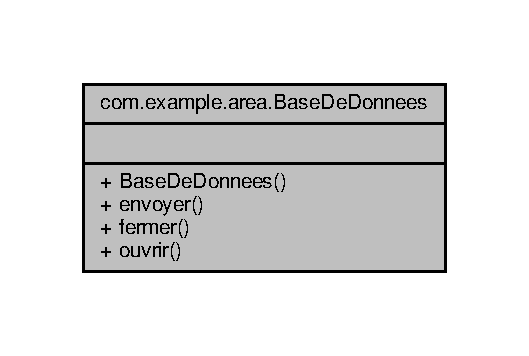
\includegraphics[width=254pt]{classcom_1_1example_1_1area_1_1_base_de_donnees__coll__graph}
\end{center}
\end{figure}
\subsubsection*{Fonctions membres publiques}
\begin{DoxyCompactItemize}
\item 
\hyperlink{classcom_1_1example_1_1area_1_1_base_de_donnees_af9165ddf75f87c6f54c08159b5f791ce}{Base\+De\+Donnees} ()
\item 
void \hyperlink{classcom_1_1example_1_1area_1_1_base_de_donnees_adf1ed72483551ccae7812eec115b9bb7}{envoyer} (String requete)
\item 
void \hyperlink{classcom_1_1example_1_1area_1_1_base_de_donnees_ad51319bd8b62ebf33d33d6f3b8347d41}{fermer} ()
\item 
void \hyperlink{classcom_1_1example_1_1area_1_1_base_de_donnees_a71c0a57c6fe4a5097e4d4c7ef1585cf3}{ouvrir} ()
\end{DoxyCompactItemize}


\subsubsection{Description détaillée}


Définition à la ligne \hyperlink{_base_de_donnees_8java_source_l00011}{11} du fichier \hyperlink{_base_de_donnees_8java_source}{Base\+De\+Donnees.\+java}.



\subsubsection{Documentation des constructeurs et destructeur}
\mbox{\Hypertarget{classcom_1_1example_1_1area_1_1_base_de_donnees_af9165ddf75f87c6f54c08159b5f791ce}\label{classcom_1_1example_1_1area_1_1_base_de_donnees_af9165ddf75f87c6f54c08159b5f791ce}} 
\index{com\+::example\+::area\+::\+Base\+De\+Donnees@{com\+::example\+::area\+::\+Base\+De\+Donnees}!Base\+De\+Donnees@{Base\+De\+Donnees}}
\index{Base\+De\+Donnees@{Base\+De\+Donnees}!com\+::example\+::area\+::\+Base\+De\+Donnees@{com\+::example\+::area\+::\+Base\+De\+Donnees}}
\paragraph{\texorpdfstring{Base\+De\+Donnees()}{BaseDeDonnees()}}
{\footnotesize\ttfamily com.\+example.\+area.\+Base\+De\+Donnees.\+Base\+De\+Donnees (\begin{DoxyParamCaption}{ }\end{DoxyParamCaption})}



Définition à la ligne \hyperlink{_base_de_donnees_8java_source_l00013}{13} du fichier \hyperlink{_base_de_donnees_8java_source}{Base\+De\+Donnees.\+java}.


\begin{DoxyCode}
00014   \{
00015   \}
\end{DoxyCode}


\subsubsection{Documentation des fonctions membres}
\mbox{\Hypertarget{classcom_1_1example_1_1area_1_1_base_de_donnees_adf1ed72483551ccae7812eec115b9bb7}\label{classcom_1_1example_1_1area_1_1_base_de_donnees_adf1ed72483551ccae7812eec115b9bb7}} 
\index{com\+::example\+::area\+::\+Base\+De\+Donnees@{com\+::example\+::area\+::\+Base\+De\+Donnees}!envoyer@{envoyer}}
\index{envoyer@{envoyer}!com\+::example\+::area\+::\+Base\+De\+Donnees@{com\+::example\+::area\+::\+Base\+De\+Donnees}}
\paragraph{\texorpdfstring{envoyer()}{envoyer()}}
{\footnotesize\ttfamily void com.\+example.\+area.\+Base\+De\+Donnees.\+envoyer (\begin{DoxyParamCaption}\item[{String}]{requete }\end{DoxyParamCaption})}



Définition à la ligne \hyperlink{_base_de_donnees_8java_source_l00025}{25} du fichier \hyperlink{_base_de_donnees_8java_source}{Base\+De\+Donnees.\+java}.


\begin{DoxyCode}
00026   \{
00027   \}
\end{DoxyCode}
\mbox{\Hypertarget{classcom_1_1example_1_1area_1_1_base_de_donnees_ad51319bd8b62ebf33d33d6f3b8347d41}\label{classcom_1_1example_1_1area_1_1_base_de_donnees_ad51319bd8b62ebf33d33d6f3b8347d41}} 
\index{com\+::example\+::area\+::\+Base\+De\+Donnees@{com\+::example\+::area\+::\+Base\+De\+Donnees}!fermer@{fermer}}
\index{fermer@{fermer}!com\+::example\+::area\+::\+Base\+De\+Donnees@{com\+::example\+::area\+::\+Base\+De\+Donnees}}
\paragraph{\texorpdfstring{fermer()}{fermer()}}
{\footnotesize\ttfamily void com.\+example.\+area.\+Base\+De\+Donnees.\+fermer (\begin{DoxyParamCaption}{ }\end{DoxyParamCaption})}



Définition à la ligne \hyperlink{_base_de_donnees_8java_source_l00021}{21} du fichier \hyperlink{_base_de_donnees_8java_source}{Base\+De\+Donnees.\+java}.


\begin{DoxyCode}
00022   \{
00023   \}
\end{DoxyCode}
\mbox{\Hypertarget{classcom_1_1example_1_1area_1_1_base_de_donnees_a71c0a57c6fe4a5097e4d4c7ef1585cf3}\label{classcom_1_1example_1_1area_1_1_base_de_donnees_a71c0a57c6fe4a5097e4d4c7ef1585cf3}} 
\index{com\+::example\+::area\+::\+Base\+De\+Donnees@{com\+::example\+::area\+::\+Base\+De\+Donnees}!ouvrir@{ouvrir}}
\index{ouvrir@{ouvrir}!com\+::example\+::area\+::\+Base\+De\+Donnees@{com\+::example\+::area\+::\+Base\+De\+Donnees}}
\paragraph{\texorpdfstring{ouvrir()}{ouvrir()}}
{\footnotesize\ttfamily void com.\+example.\+area.\+Base\+De\+Donnees.\+ouvrir (\begin{DoxyParamCaption}{ }\end{DoxyParamCaption})}



Définition à la ligne \hyperlink{_base_de_donnees_8java_source_l00017}{17} du fichier \hyperlink{_base_de_donnees_8java_source}{Base\+De\+Donnees.\+java}.


\begin{DoxyCode}
00018   \{
00019   \}
\end{DoxyCode}


La documentation de cette classe a été générée à partir du fichier suivant \+:\begin{DoxyCompactItemize}
\item 
\hyperlink{_base_de_donnees_8java}{Base\+De\+Donnees.\+java}\end{DoxyCompactItemize}

\hypertarget{classcom_1_1example_1_1area_1_1_equipe}{}\subsection{Référence de la classe com.\+example.\+area.\+Equipe}
\label{classcom_1_1example_1_1area_1_1_equipe}\index{com.\+example.\+area.\+Equipe@{com.\+example.\+area.\+Equipe}}


Graphe de collaboration de com.\+example.\+area.\+Equipe\+:
\nopagebreak
\begin{figure}[H]
\begin{center}
\leavevmode
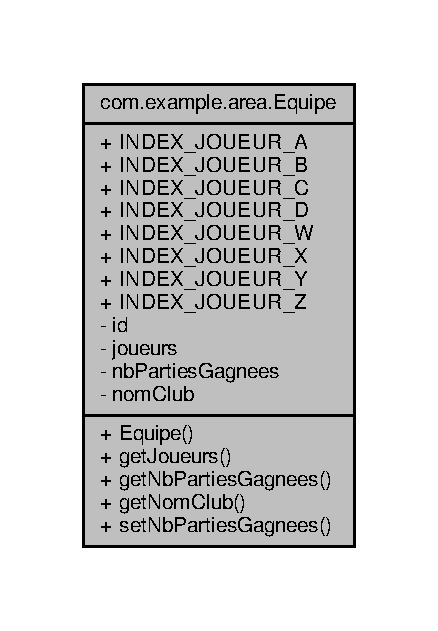
\includegraphics[width=210pt]{classcom_1_1example_1_1area_1_1_equipe__coll__graph}
\end{center}
\end{figure}
\subsubsection*{Fonctions membres publiques}
\begin{DoxyCompactItemize}
\item 
\hyperlink{classcom_1_1example_1_1area_1_1_equipe_a313ec6933f3fb30f68ec93c7c290c6ee}{Equipe} (String \hyperlink{classcom_1_1example_1_1area_1_1_equipe_ac93205e041df88192dd6b1dfc8488e0a}{nom\+Club}, Vector$<$ \hyperlink{classcom_1_1example_1_1area_1_1_joueur}{Joueur} $>$ \hyperlink{classcom_1_1example_1_1area_1_1_equipe_a13f5e9288dec5f11829e1a7ccc21cdc9}{joueurs})
\item 
Vector$<$ \hyperlink{classcom_1_1example_1_1area_1_1_joueur}{Joueur} $>$ \hyperlink{classcom_1_1example_1_1area_1_1_equipe_aa681b4ea72d93a16fc8384fa3ccc8b21}{get\+Joueurs} ()
\item 
final int \hyperlink{classcom_1_1example_1_1area_1_1_equipe_a1ba6f14b9b168e283d5d6417ad0a5ed2}{get\+Nb\+Parties\+Gagnees} ()
\item 
final String \hyperlink{classcom_1_1example_1_1area_1_1_equipe_a735e5e0aaac9ac2c17f3eca3d47862dc}{get\+Nom\+Club} ()
\item 
void \hyperlink{classcom_1_1example_1_1area_1_1_equipe_aba16e2f2a922d1b2c4219dc6c865482c}{set\+Nb\+Parties\+Gagnees} (int \hyperlink{classcom_1_1example_1_1area_1_1_equipe_af01e154be3aaa3fbcf909c3a44734b2e}{nb\+Parties\+Gagnees})
\end{DoxyCompactItemize}
\subsubsection*{Attributs publics statiques}
\begin{DoxyCompactItemize}
\item 
static final int \hyperlink{classcom_1_1example_1_1area_1_1_equipe_a3b61c78bfb4284470bc3b5315b6b03e7}{I\+N\+D\+E\+X\+\_\+\+J\+O\+U\+E\+U\+R\+\_\+A} = 0
\item 
static final int \hyperlink{classcom_1_1example_1_1area_1_1_equipe_a1b9c3f1c23757be40472c63504df9d37}{I\+N\+D\+E\+X\+\_\+\+J\+O\+U\+E\+U\+R\+\_\+B} = 1
\item 
static final int \hyperlink{classcom_1_1example_1_1area_1_1_equipe_abbd44b4789c0234d86578fbbfd8bf624}{I\+N\+D\+E\+X\+\_\+\+J\+O\+U\+E\+U\+R\+\_\+C} = 2
\item 
static final int \hyperlink{classcom_1_1example_1_1area_1_1_equipe_ae204f48df7446d745f33ff4a7e662ea7}{I\+N\+D\+E\+X\+\_\+\+J\+O\+U\+E\+U\+R\+\_\+D} = 3
\item 
static final int \hyperlink{classcom_1_1example_1_1area_1_1_equipe_aeca3d6f47e05b7c2aef70b64778d5d47}{I\+N\+D\+E\+X\+\_\+\+J\+O\+U\+E\+U\+R\+\_\+W} = 0
\item 
static final int \hyperlink{classcom_1_1example_1_1area_1_1_equipe_ae5f0313dce371f13950d4fdc54074dd9}{I\+N\+D\+E\+X\+\_\+\+J\+O\+U\+E\+U\+R\+\_\+X} = 1
\item 
static final int \hyperlink{classcom_1_1example_1_1area_1_1_equipe_a11d252140fc4e3edd71a31573221a7b7}{I\+N\+D\+E\+X\+\_\+\+J\+O\+U\+E\+U\+R\+\_\+Y} = 2
\item 
static final int \hyperlink{classcom_1_1example_1_1area_1_1_equipe_a50e1c2cbd7d24c8c5b4f0f4de1652621}{I\+N\+D\+E\+X\+\_\+\+J\+O\+U\+E\+U\+R\+\_\+Z} = 3
\end{DoxyCompactItemize}
\subsubsection*{Attributs privés}
\begin{DoxyCompactItemize}
\item 
int \hyperlink{classcom_1_1example_1_1area_1_1_equipe_a3be17f443cb57269d595d8b860acc66a}{id}
\item 
Vector$<$ \hyperlink{classcom_1_1example_1_1area_1_1_joueur}{Joueur} $>$ \hyperlink{classcom_1_1example_1_1area_1_1_equipe_a13f5e9288dec5f11829e1a7ccc21cdc9}{joueurs}
\item 
int \hyperlink{classcom_1_1example_1_1area_1_1_equipe_af01e154be3aaa3fbcf909c3a44734b2e}{nb\+Parties\+Gagnees}
\item 
String \hyperlink{classcom_1_1example_1_1area_1_1_equipe_ac93205e041df88192dd6b1dfc8488e0a}{nom\+Club}
\end{DoxyCompactItemize}


\subsubsection{Description détaillée}


Définition à la ligne \hyperlink{_equipe_8java_source_l00013}{13} du fichier \hyperlink{_equipe_8java_source}{Equipe.\+java}.



\subsubsection{Documentation des constructeurs et destructeur}
\mbox{\Hypertarget{classcom_1_1example_1_1area_1_1_equipe_a313ec6933f3fb30f68ec93c7c290c6ee}\label{classcom_1_1example_1_1area_1_1_equipe_a313ec6933f3fb30f68ec93c7c290c6ee}} 
\index{com\+::example\+::area\+::\+Equipe@{com\+::example\+::area\+::\+Equipe}!Equipe@{Equipe}}
\index{Equipe@{Equipe}!com\+::example\+::area\+::\+Equipe@{com\+::example\+::area\+::\+Equipe}}
\paragraph{\texorpdfstring{Equipe()}{Equipe()}}
{\footnotesize\ttfamily com.\+example.\+area.\+Equipe.\+Equipe (\begin{DoxyParamCaption}\item[{String}]{nom\+Club,  }\item[{Vector$<$ \hyperlink{classcom_1_1example_1_1area_1_1_joueur}{Joueur} $>$}]{joueurs }\end{DoxyParamCaption})}



Définition à la ligne \hyperlink{_equipe_8java_source_l00030}{30} du fichier \hyperlink{_equipe_8java_source}{Equipe.\+java}.



Références \hyperlink{_equipe_8java_source_l00027}{com.\+example.\+area.\+Equipe.\+joueurs}, et \hyperlink{_equipe_8java_source_l00026}{com.\+example.\+area.\+Equipe.\+nom\+Club}.


\begin{DoxyCode}
00031     \{
00032         this.\hyperlink{classcom_1_1example_1_1area_1_1_equipe_af01e154be3aaa3fbcf909c3a44734b2e}{nbPartiesGagnees} = 0;
00033         this.\hyperlink{classcom_1_1example_1_1area_1_1_equipe_ac93205e041df88192dd6b1dfc8488e0a}{nomClub} = \hyperlink{classcom_1_1example_1_1area_1_1_equipe_ac93205e041df88192dd6b1dfc8488e0a}{nomClub};
00034         this.\hyperlink{classcom_1_1example_1_1area_1_1_equipe_a13f5e9288dec5f11829e1a7ccc21cdc9}{joueurs} = \hyperlink{classcom_1_1example_1_1area_1_1_equipe_a13f5e9288dec5f11829e1a7ccc21cdc9}{joueurs};
00035         this.\textcolor{keywordtype}{id} = 0;
00036     \}
\end{DoxyCode}


\subsubsection{Documentation des fonctions membres}
\mbox{\Hypertarget{classcom_1_1example_1_1area_1_1_equipe_aa681b4ea72d93a16fc8384fa3ccc8b21}\label{classcom_1_1example_1_1area_1_1_equipe_aa681b4ea72d93a16fc8384fa3ccc8b21}} 
\index{com\+::example\+::area\+::\+Equipe@{com\+::example\+::area\+::\+Equipe}!get\+Joueurs@{get\+Joueurs}}
\index{get\+Joueurs@{get\+Joueurs}!com\+::example\+::area\+::\+Equipe@{com\+::example\+::area\+::\+Equipe}}
\paragraph{\texorpdfstring{get\+Joueurs()}{getJoueurs()}}
{\footnotesize\ttfamily Vector$<$\hyperlink{classcom_1_1example_1_1area_1_1_joueur}{Joueur}$>$ com.\+example.\+area.\+Equipe.\+get\+Joueurs (\begin{DoxyParamCaption}{ }\end{DoxyParamCaption})}



Définition à la ligne \hyperlink{_equipe_8java_source_l00053}{53} du fichier \hyperlink{_equipe_8java_source}{Equipe.\+java}.



Références \hyperlink{_equipe_8java_source_l00027}{com.\+example.\+area.\+Equipe.\+joueurs}.


\begin{DoxyCode}
00054     \{
00055         \textcolor{keywordflow}{return} \hyperlink{classcom_1_1example_1_1area_1_1_equipe_a13f5e9288dec5f11829e1a7ccc21cdc9}{joueurs};
00056     \}
\end{DoxyCode}
\mbox{\Hypertarget{classcom_1_1example_1_1area_1_1_equipe_a1ba6f14b9b168e283d5d6417ad0a5ed2}\label{classcom_1_1example_1_1area_1_1_equipe_a1ba6f14b9b168e283d5d6417ad0a5ed2}} 
\index{com\+::example\+::area\+::\+Equipe@{com\+::example\+::area\+::\+Equipe}!get\+Nb\+Parties\+Gagnees@{get\+Nb\+Parties\+Gagnees}}
\index{get\+Nb\+Parties\+Gagnees@{get\+Nb\+Parties\+Gagnees}!com\+::example\+::area\+::\+Equipe@{com\+::example\+::area\+::\+Equipe}}
\paragraph{\texorpdfstring{get\+Nb\+Parties\+Gagnees()}{getNbPartiesGagnees()}}
{\footnotesize\ttfamily final int com.\+example.\+area.\+Equipe.\+get\+Nb\+Parties\+Gagnees (\begin{DoxyParamCaption}{ }\end{DoxyParamCaption})}



Définition à la ligne \hyperlink{_equipe_8java_source_l00038}{38} du fichier \hyperlink{_equipe_8java_source}{Equipe.\+java}.



Références \hyperlink{_equipe_8java_source_l00025}{com.\+example.\+area.\+Equipe.\+nb\+Parties\+Gagnees}.


\begin{DoxyCode}
00039     \{
00040       \textcolor{keywordflow}{return} \hyperlink{classcom_1_1example_1_1area_1_1_equipe_af01e154be3aaa3fbcf909c3a44734b2e}{nbPartiesGagnees};
00041     \}
\end{DoxyCode}
\mbox{\Hypertarget{classcom_1_1example_1_1area_1_1_equipe_a735e5e0aaac9ac2c17f3eca3d47862dc}\label{classcom_1_1example_1_1area_1_1_equipe_a735e5e0aaac9ac2c17f3eca3d47862dc}} 
\index{com\+::example\+::area\+::\+Equipe@{com\+::example\+::area\+::\+Equipe}!get\+Nom\+Club@{get\+Nom\+Club}}
\index{get\+Nom\+Club@{get\+Nom\+Club}!com\+::example\+::area\+::\+Equipe@{com\+::example\+::area\+::\+Equipe}}
\paragraph{\texorpdfstring{get\+Nom\+Club()}{getNomClub()}}
{\footnotesize\ttfamily final String com.\+example.\+area.\+Equipe.\+get\+Nom\+Club (\begin{DoxyParamCaption}{ }\end{DoxyParamCaption})}



Définition à la ligne \hyperlink{_equipe_8java_source_l00043}{43} du fichier \hyperlink{_equipe_8java_source}{Equipe.\+java}.



Références \hyperlink{_equipe_8java_source_l00026}{com.\+example.\+area.\+Equipe.\+nom\+Club}.



Référencé par \hyperlink{_i_h_m_gestion_rencontre_8java_source_l00142}{com.\+example.\+area.\+I\+H\+M\+Gestion\+Rencontre.\+initialiser\+Ressources\+I\+H\+M()}, et \hyperlink{_i_h_m_gestion_rencontre_8java_source_l00281}{com.\+example.\+area.\+I\+H\+M\+Gestion\+Rencontre.\+recuperer\+Noms\+Joueurs()}.


\begin{DoxyCode}
00044     \{
00045       \textcolor{keywordflow}{return} \hyperlink{classcom_1_1example_1_1area_1_1_equipe_ac93205e041df88192dd6b1dfc8488e0a}{nomClub};
00046     \}
\end{DoxyCode}
\mbox{\Hypertarget{classcom_1_1example_1_1area_1_1_equipe_aba16e2f2a922d1b2c4219dc6c865482c}\label{classcom_1_1example_1_1area_1_1_equipe_aba16e2f2a922d1b2c4219dc6c865482c}} 
\index{com\+::example\+::area\+::\+Equipe@{com\+::example\+::area\+::\+Equipe}!set\+Nb\+Parties\+Gagnees@{set\+Nb\+Parties\+Gagnees}}
\index{set\+Nb\+Parties\+Gagnees@{set\+Nb\+Parties\+Gagnees}!com\+::example\+::area\+::\+Equipe@{com\+::example\+::area\+::\+Equipe}}
\paragraph{\texorpdfstring{set\+Nb\+Parties\+Gagnees()}{setNbPartiesGagnees()}}
{\footnotesize\ttfamily void com.\+example.\+area.\+Equipe.\+set\+Nb\+Parties\+Gagnees (\begin{DoxyParamCaption}\item[{int}]{nb\+Parties\+Gagnees }\end{DoxyParamCaption})}



Définition à la ligne \hyperlink{_equipe_8java_source_l00048}{48} du fichier \hyperlink{_equipe_8java_source}{Equipe.\+java}.



Références \hyperlink{_equipe_8java_source_l00025}{com.\+example.\+area.\+Equipe.\+nb\+Parties\+Gagnees}.


\begin{DoxyCode}
00049     \{
00050       this.\hyperlink{classcom_1_1example_1_1area_1_1_equipe_af01e154be3aaa3fbcf909c3a44734b2e}{nbPartiesGagnees} = \hyperlink{classcom_1_1example_1_1area_1_1_equipe_af01e154be3aaa3fbcf909c3a44734b2e}{nbPartiesGagnees};
00051     \}
\end{DoxyCode}


\subsubsection{Documentation des données membres}
\mbox{\Hypertarget{classcom_1_1example_1_1area_1_1_equipe_a3be17f443cb57269d595d8b860acc66a}\label{classcom_1_1example_1_1area_1_1_equipe_a3be17f443cb57269d595d8b860acc66a}} 
\index{com\+::example\+::area\+::\+Equipe@{com\+::example\+::area\+::\+Equipe}!id@{id}}
\index{id@{id}!com\+::example\+::area\+::\+Equipe@{com\+::example\+::area\+::\+Equipe}}
\paragraph{\texorpdfstring{id}{id}}
{\footnotesize\ttfamily int com.\+example.\+area.\+Equipe.\+id\hspace{0.3cm}{\ttfamily [private]}}



Définition à la ligne \hyperlink{_equipe_8java_source_l00028}{28} du fichier \hyperlink{_equipe_8java_source}{Equipe.\+java}.

\mbox{\Hypertarget{classcom_1_1example_1_1area_1_1_equipe_a3b61c78bfb4284470bc3b5315b6b03e7}\label{classcom_1_1example_1_1area_1_1_equipe_a3b61c78bfb4284470bc3b5315b6b03e7}} 
\index{com\+::example\+::area\+::\+Equipe@{com\+::example\+::area\+::\+Equipe}!I\+N\+D\+E\+X\+\_\+\+J\+O\+U\+E\+U\+R\+\_\+A@{I\+N\+D\+E\+X\+\_\+\+J\+O\+U\+E\+U\+R\+\_\+A}}
\index{I\+N\+D\+E\+X\+\_\+\+J\+O\+U\+E\+U\+R\+\_\+A@{I\+N\+D\+E\+X\+\_\+\+J\+O\+U\+E\+U\+R\+\_\+A}!com\+::example\+::area\+::\+Equipe@{com\+::example\+::area\+::\+Equipe}}
\paragraph{\texorpdfstring{I\+N\+D\+E\+X\+\_\+\+J\+O\+U\+E\+U\+R\+\_\+A}{INDEX\_JOUEUR\_A}}
{\footnotesize\ttfamily final int com.\+example.\+area.\+Equipe.\+I\+N\+D\+E\+X\+\_\+\+J\+O\+U\+E\+U\+R\+\_\+A = 0\hspace{0.3cm}{\ttfamily [static]}}



Définition à la ligne \hyperlink{_equipe_8java_source_l00015}{15} du fichier \hyperlink{_equipe_8java_source}{Equipe.\+java}.



Référencé par \hyperlink{_rencontre_8java_source_l00081}{com.\+example.\+area.\+Rencontre.\+initialiser\+Parties()}.

\mbox{\Hypertarget{classcom_1_1example_1_1area_1_1_equipe_a1b9c3f1c23757be40472c63504df9d37}\label{classcom_1_1example_1_1area_1_1_equipe_a1b9c3f1c23757be40472c63504df9d37}} 
\index{com\+::example\+::area\+::\+Equipe@{com\+::example\+::area\+::\+Equipe}!I\+N\+D\+E\+X\+\_\+\+J\+O\+U\+E\+U\+R\+\_\+B@{I\+N\+D\+E\+X\+\_\+\+J\+O\+U\+E\+U\+R\+\_\+B}}
\index{I\+N\+D\+E\+X\+\_\+\+J\+O\+U\+E\+U\+R\+\_\+B@{I\+N\+D\+E\+X\+\_\+\+J\+O\+U\+E\+U\+R\+\_\+B}!com\+::example\+::area\+::\+Equipe@{com\+::example\+::area\+::\+Equipe}}
\paragraph{\texorpdfstring{I\+N\+D\+E\+X\+\_\+\+J\+O\+U\+E\+U\+R\+\_\+B}{INDEX\_JOUEUR\_B}}
{\footnotesize\ttfamily final int com.\+example.\+area.\+Equipe.\+I\+N\+D\+E\+X\+\_\+\+J\+O\+U\+E\+U\+R\+\_\+B = 1\hspace{0.3cm}{\ttfamily [static]}}



Définition à la ligne \hyperlink{_equipe_8java_source_l00016}{16} du fichier \hyperlink{_equipe_8java_source}{Equipe.\+java}.



Référencé par \hyperlink{_rencontre_8java_source_l00081}{com.\+example.\+area.\+Rencontre.\+initialiser\+Parties()}.

\mbox{\Hypertarget{classcom_1_1example_1_1area_1_1_equipe_abbd44b4789c0234d86578fbbfd8bf624}\label{classcom_1_1example_1_1area_1_1_equipe_abbd44b4789c0234d86578fbbfd8bf624}} 
\index{com\+::example\+::area\+::\+Equipe@{com\+::example\+::area\+::\+Equipe}!I\+N\+D\+E\+X\+\_\+\+J\+O\+U\+E\+U\+R\+\_\+C@{I\+N\+D\+E\+X\+\_\+\+J\+O\+U\+E\+U\+R\+\_\+C}}
\index{I\+N\+D\+E\+X\+\_\+\+J\+O\+U\+E\+U\+R\+\_\+C@{I\+N\+D\+E\+X\+\_\+\+J\+O\+U\+E\+U\+R\+\_\+C}!com\+::example\+::area\+::\+Equipe@{com\+::example\+::area\+::\+Equipe}}
\paragraph{\texorpdfstring{I\+N\+D\+E\+X\+\_\+\+J\+O\+U\+E\+U\+R\+\_\+C}{INDEX\_JOUEUR\_C}}
{\footnotesize\ttfamily final int com.\+example.\+area.\+Equipe.\+I\+N\+D\+E\+X\+\_\+\+J\+O\+U\+E\+U\+R\+\_\+C = 2\hspace{0.3cm}{\ttfamily [static]}}



Définition à la ligne \hyperlink{_equipe_8java_source_l00017}{17} du fichier \hyperlink{_equipe_8java_source}{Equipe.\+java}.



Référencé par \hyperlink{_rencontre_8java_source_l00081}{com.\+example.\+area.\+Rencontre.\+initialiser\+Parties()}.

\mbox{\Hypertarget{classcom_1_1example_1_1area_1_1_equipe_ae204f48df7446d745f33ff4a7e662ea7}\label{classcom_1_1example_1_1area_1_1_equipe_ae204f48df7446d745f33ff4a7e662ea7}} 
\index{com\+::example\+::area\+::\+Equipe@{com\+::example\+::area\+::\+Equipe}!I\+N\+D\+E\+X\+\_\+\+J\+O\+U\+E\+U\+R\+\_\+D@{I\+N\+D\+E\+X\+\_\+\+J\+O\+U\+E\+U\+R\+\_\+D}}
\index{I\+N\+D\+E\+X\+\_\+\+J\+O\+U\+E\+U\+R\+\_\+D@{I\+N\+D\+E\+X\+\_\+\+J\+O\+U\+E\+U\+R\+\_\+D}!com\+::example\+::area\+::\+Equipe@{com\+::example\+::area\+::\+Equipe}}
\paragraph{\texorpdfstring{I\+N\+D\+E\+X\+\_\+\+J\+O\+U\+E\+U\+R\+\_\+D}{INDEX\_JOUEUR\_D}}
{\footnotesize\ttfamily final int com.\+example.\+area.\+Equipe.\+I\+N\+D\+E\+X\+\_\+\+J\+O\+U\+E\+U\+R\+\_\+D = 3\hspace{0.3cm}{\ttfamily [static]}}



Définition à la ligne \hyperlink{_equipe_8java_source_l00018}{18} du fichier \hyperlink{_equipe_8java_source}{Equipe.\+java}.



Référencé par \hyperlink{_rencontre_8java_source_l00081}{com.\+example.\+area.\+Rencontre.\+initialiser\+Parties()}.

\mbox{\Hypertarget{classcom_1_1example_1_1area_1_1_equipe_aeca3d6f47e05b7c2aef70b64778d5d47}\label{classcom_1_1example_1_1area_1_1_equipe_aeca3d6f47e05b7c2aef70b64778d5d47}} 
\index{com\+::example\+::area\+::\+Equipe@{com\+::example\+::area\+::\+Equipe}!I\+N\+D\+E\+X\+\_\+\+J\+O\+U\+E\+U\+R\+\_\+W@{I\+N\+D\+E\+X\+\_\+\+J\+O\+U\+E\+U\+R\+\_\+W}}
\index{I\+N\+D\+E\+X\+\_\+\+J\+O\+U\+E\+U\+R\+\_\+W@{I\+N\+D\+E\+X\+\_\+\+J\+O\+U\+E\+U\+R\+\_\+W}!com\+::example\+::area\+::\+Equipe@{com\+::example\+::area\+::\+Equipe}}
\paragraph{\texorpdfstring{I\+N\+D\+E\+X\+\_\+\+J\+O\+U\+E\+U\+R\+\_\+W}{INDEX\_JOUEUR\_W}}
{\footnotesize\ttfamily final int com.\+example.\+area.\+Equipe.\+I\+N\+D\+E\+X\+\_\+\+J\+O\+U\+E\+U\+R\+\_\+W = 0\hspace{0.3cm}{\ttfamily [static]}}



Définition à la ligne \hyperlink{_equipe_8java_source_l00020}{20} du fichier \hyperlink{_equipe_8java_source}{Equipe.\+java}.



Référencé par \hyperlink{_rencontre_8java_source_l00081}{com.\+example.\+area.\+Rencontre.\+initialiser\+Parties()}.

\mbox{\Hypertarget{classcom_1_1example_1_1area_1_1_equipe_ae5f0313dce371f13950d4fdc54074dd9}\label{classcom_1_1example_1_1area_1_1_equipe_ae5f0313dce371f13950d4fdc54074dd9}} 
\index{com\+::example\+::area\+::\+Equipe@{com\+::example\+::area\+::\+Equipe}!I\+N\+D\+E\+X\+\_\+\+J\+O\+U\+E\+U\+R\+\_\+X@{I\+N\+D\+E\+X\+\_\+\+J\+O\+U\+E\+U\+R\+\_\+X}}
\index{I\+N\+D\+E\+X\+\_\+\+J\+O\+U\+E\+U\+R\+\_\+X@{I\+N\+D\+E\+X\+\_\+\+J\+O\+U\+E\+U\+R\+\_\+X}!com\+::example\+::area\+::\+Equipe@{com\+::example\+::area\+::\+Equipe}}
\paragraph{\texorpdfstring{I\+N\+D\+E\+X\+\_\+\+J\+O\+U\+E\+U\+R\+\_\+X}{INDEX\_JOUEUR\_X}}
{\footnotesize\ttfamily final int com.\+example.\+area.\+Equipe.\+I\+N\+D\+E\+X\+\_\+\+J\+O\+U\+E\+U\+R\+\_\+X = 1\hspace{0.3cm}{\ttfamily [static]}}



Définition à la ligne \hyperlink{_equipe_8java_source_l00021}{21} du fichier \hyperlink{_equipe_8java_source}{Equipe.\+java}.



Référencé par \hyperlink{_rencontre_8java_source_l00081}{com.\+example.\+area.\+Rencontre.\+initialiser\+Parties()}.

\mbox{\Hypertarget{classcom_1_1example_1_1area_1_1_equipe_a11d252140fc4e3edd71a31573221a7b7}\label{classcom_1_1example_1_1area_1_1_equipe_a11d252140fc4e3edd71a31573221a7b7}} 
\index{com\+::example\+::area\+::\+Equipe@{com\+::example\+::area\+::\+Equipe}!I\+N\+D\+E\+X\+\_\+\+J\+O\+U\+E\+U\+R\+\_\+Y@{I\+N\+D\+E\+X\+\_\+\+J\+O\+U\+E\+U\+R\+\_\+Y}}
\index{I\+N\+D\+E\+X\+\_\+\+J\+O\+U\+E\+U\+R\+\_\+Y@{I\+N\+D\+E\+X\+\_\+\+J\+O\+U\+E\+U\+R\+\_\+Y}!com\+::example\+::area\+::\+Equipe@{com\+::example\+::area\+::\+Equipe}}
\paragraph{\texorpdfstring{I\+N\+D\+E\+X\+\_\+\+J\+O\+U\+E\+U\+R\+\_\+Y}{INDEX\_JOUEUR\_Y}}
{\footnotesize\ttfamily final int com.\+example.\+area.\+Equipe.\+I\+N\+D\+E\+X\+\_\+\+J\+O\+U\+E\+U\+R\+\_\+Y = 2\hspace{0.3cm}{\ttfamily [static]}}



Définition à la ligne \hyperlink{_equipe_8java_source_l00022}{22} du fichier \hyperlink{_equipe_8java_source}{Equipe.\+java}.



Référencé par \hyperlink{_rencontre_8java_source_l00081}{com.\+example.\+area.\+Rencontre.\+initialiser\+Parties()}.

\mbox{\Hypertarget{classcom_1_1example_1_1area_1_1_equipe_a50e1c2cbd7d24c8c5b4f0f4de1652621}\label{classcom_1_1example_1_1area_1_1_equipe_a50e1c2cbd7d24c8c5b4f0f4de1652621}} 
\index{com\+::example\+::area\+::\+Equipe@{com\+::example\+::area\+::\+Equipe}!I\+N\+D\+E\+X\+\_\+\+J\+O\+U\+E\+U\+R\+\_\+Z@{I\+N\+D\+E\+X\+\_\+\+J\+O\+U\+E\+U\+R\+\_\+Z}}
\index{I\+N\+D\+E\+X\+\_\+\+J\+O\+U\+E\+U\+R\+\_\+Z@{I\+N\+D\+E\+X\+\_\+\+J\+O\+U\+E\+U\+R\+\_\+Z}!com\+::example\+::area\+::\+Equipe@{com\+::example\+::area\+::\+Equipe}}
\paragraph{\texorpdfstring{I\+N\+D\+E\+X\+\_\+\+J\+O\+U\+E\+U\+R\+\_\+Z}{INDEX\_JOUEUR\_Z}}
{\footnotesize\ttfamily final int com.\+example.\+area.\+Equipe.\+I\+N\+D\+E\+X\+\_\+\+J\+O\+U\+E\+U\+R\+\_\+Z = 3\hspace{0.3cm}{\ttfamily [static]}}



Définition à la ligne \hyperlink{_equipe_8java_source_l00023}{23} du fichier \hyperlink{_equipe_8java_source}{Equipe.\+java}.



Référencé par \hyperlink{_rencontre_8java_source_l00081}{com.\+example.\+area.\+Rencontre.\+initialiser\+Parties()}.

\mbox{\Hypertarget{classcom_1_1example_1_1area_1_1_equipe_a13f5e9288dec5f11829e1a7ccc21cdc9}\label{classcom_1_1example_1_1area_1_1_equipe_a13f5e9288dec5f11829e1a7ccc21cdc9}} 
\index{com\+::example\+::area\+::\+Equipe@{com\+::example\+::area\+::\+Equipe}!joueurs@{joueurs}}
\index{joueurs@{joueurs}!com\+::example\+::area\+::\+Equipe@{com\+::example\+::area\+::\+Equipe}}
\paragraph{\texorpdfstring{joueurs}{joueurs}}
{\footnotesize\ttfamily Vector$<$\hyperlink{classcom_1_1example_1_1area_1_1_joueur}{Joueur}$>$ com.\+example.\+area.\+Equipe.\+joueurs\hspace{0.3cm}{\ttfamily [private]}}



Définition à la ligne \hyperlink{_equipe_8java_source_l00027}{27} du fichier \hyperlink{_equipe_8java_source}{Equipe.\+java}.



Référencé par \hyperlink{_equipe_8java_source_l00030}{com.\+example.\+area.\+Equipe.\+Equipe()}, et \hyperlink{_equipe_8java_source_l00053}{com.\+example.\+area.\+Equipe.\+get\+Joueurs()}.

\mbox{\Hypertarget{classcom_1_1example_1_1area_1_1_equipe_af01e154be3aaa3fbcf909c3a44734b2e}\label{classcom_1_1example_1_1area_1_1_equipe_af01e154be3aaa3fbcf909c3a44734b2e}} 
\index{com\+::example\+::area\+::\+Equipe@{com\+::example\+::area\+::\+Equipe}!nb\+Parties\+Gagnees@{nb\+Parties\+Gagnees}}
\index{nb\+Parties\+Gagnees@{nb\+Parties\+Gagnees}!com\+::example\+::area\+::\+Equipe@{com\+::example\+::area\+::\+Equipe}}
\paragraph{\texorpdfstring{nb\+Parties\+Gagnees}{nbPartiesGagnees}}
{\footnotesize\ttfamily int com.\+example.\+area.\+Equipe.\+nb\+Parties\+Gagnees\hspace{0.3cm}{\ttfamily [private]}}



Définition à la ligne \hyperlink{_equipe_8java_source_l00025}{25} du fichier \hyperlink{_equipe_8java_source}{Equipe.\+java}.



Référencé par \hyperlink{_equipe_8java_source_l00038}{com.\+example.\+area.\+Equipe.\+get\+Nb\+Parties\+Gagnees()}, et \hyperlink{_equipe_8java_source_l00048}{com.\+example.\+area.\+Equipe.\+set\+Nb\+Parties\+Gagnees()}.

\mbox{\Hypertarget{classcom_1_1example_1_1area_1_1_equipe_ac93205e041df88192dd6b1dfc8488e0a}\label{classcom_1_1example_1_1area_1_1_equipe_ac93205e041df88192dd6b1dfc8488e0a}} 
\index{com\+::example\+::area\+::\+Equipe@{com\+::example\+::area\+::\+Equipe}!nom\+Club@{nom\+Club}}
\index{nom\+Club@{nom\+Club}!com\+::example\+::area\+::\+Equipe@{com\+::example\+::area\+::\+Equipe}}
\paragraph{\texorpdfstring{nom\+Club}{nomClub}}
{\footnotesize\ttfamily String com.\+example.\+area.\+Equipe.\+nom\+Club\hspace{0.3cm}{\ttfamily [private]}}



Définition à la ligne \hyperlink{_equipe_8java_source_l00026}{26} du fichier \hyperlink{_equipe_8java_source}{Equipe.\+java}.



Référencé par \hyperlink{_equipe_8java_source_l00030}{com.\+example.\+area.\+Equipe.\+Equipe()}, et \hyperlink{_equipe_8java_source_l00043}{com.\+example.\+area.\+Equipe.\+get\+Nom\+Club()}.



La documentation de cette classe a été générée à partir du fichier suivant \+:\begin{DoxyCompactItemize}
\item 
\hyperlink{_equipe_8java}{Equipe.\+java}\end{DoxyCompactItemize}

\hypertarget{classcom_1_1example_1_1area_1_1_i_h_m_gestion_partie}{}\subsection{Référence de la classe com.\+example.\+area.\+I\+H\+M\+Gestion\+Partie}
\label{classcom_1_1example_1_1area_1_1_i_h_m_gestion_partie}\index{com.\+example.\+area.\+I\+H\+M\+Gestion\+Partie@{com.\+example.\+area.\+I\+H\+M\+Gestion\+Partie}}


L\textquotesingle{}activité de gestion d\textquotesingle{}une partie de l\textquotesingle{}application A\+R\+EA.  




Graphe de collaboration de com.\+example.\+area.\+I\+H\+M\+Gestion\+Partie\+:
\nopagebreak
\begin{figure}[H]
\begin{center}
\leavevmode
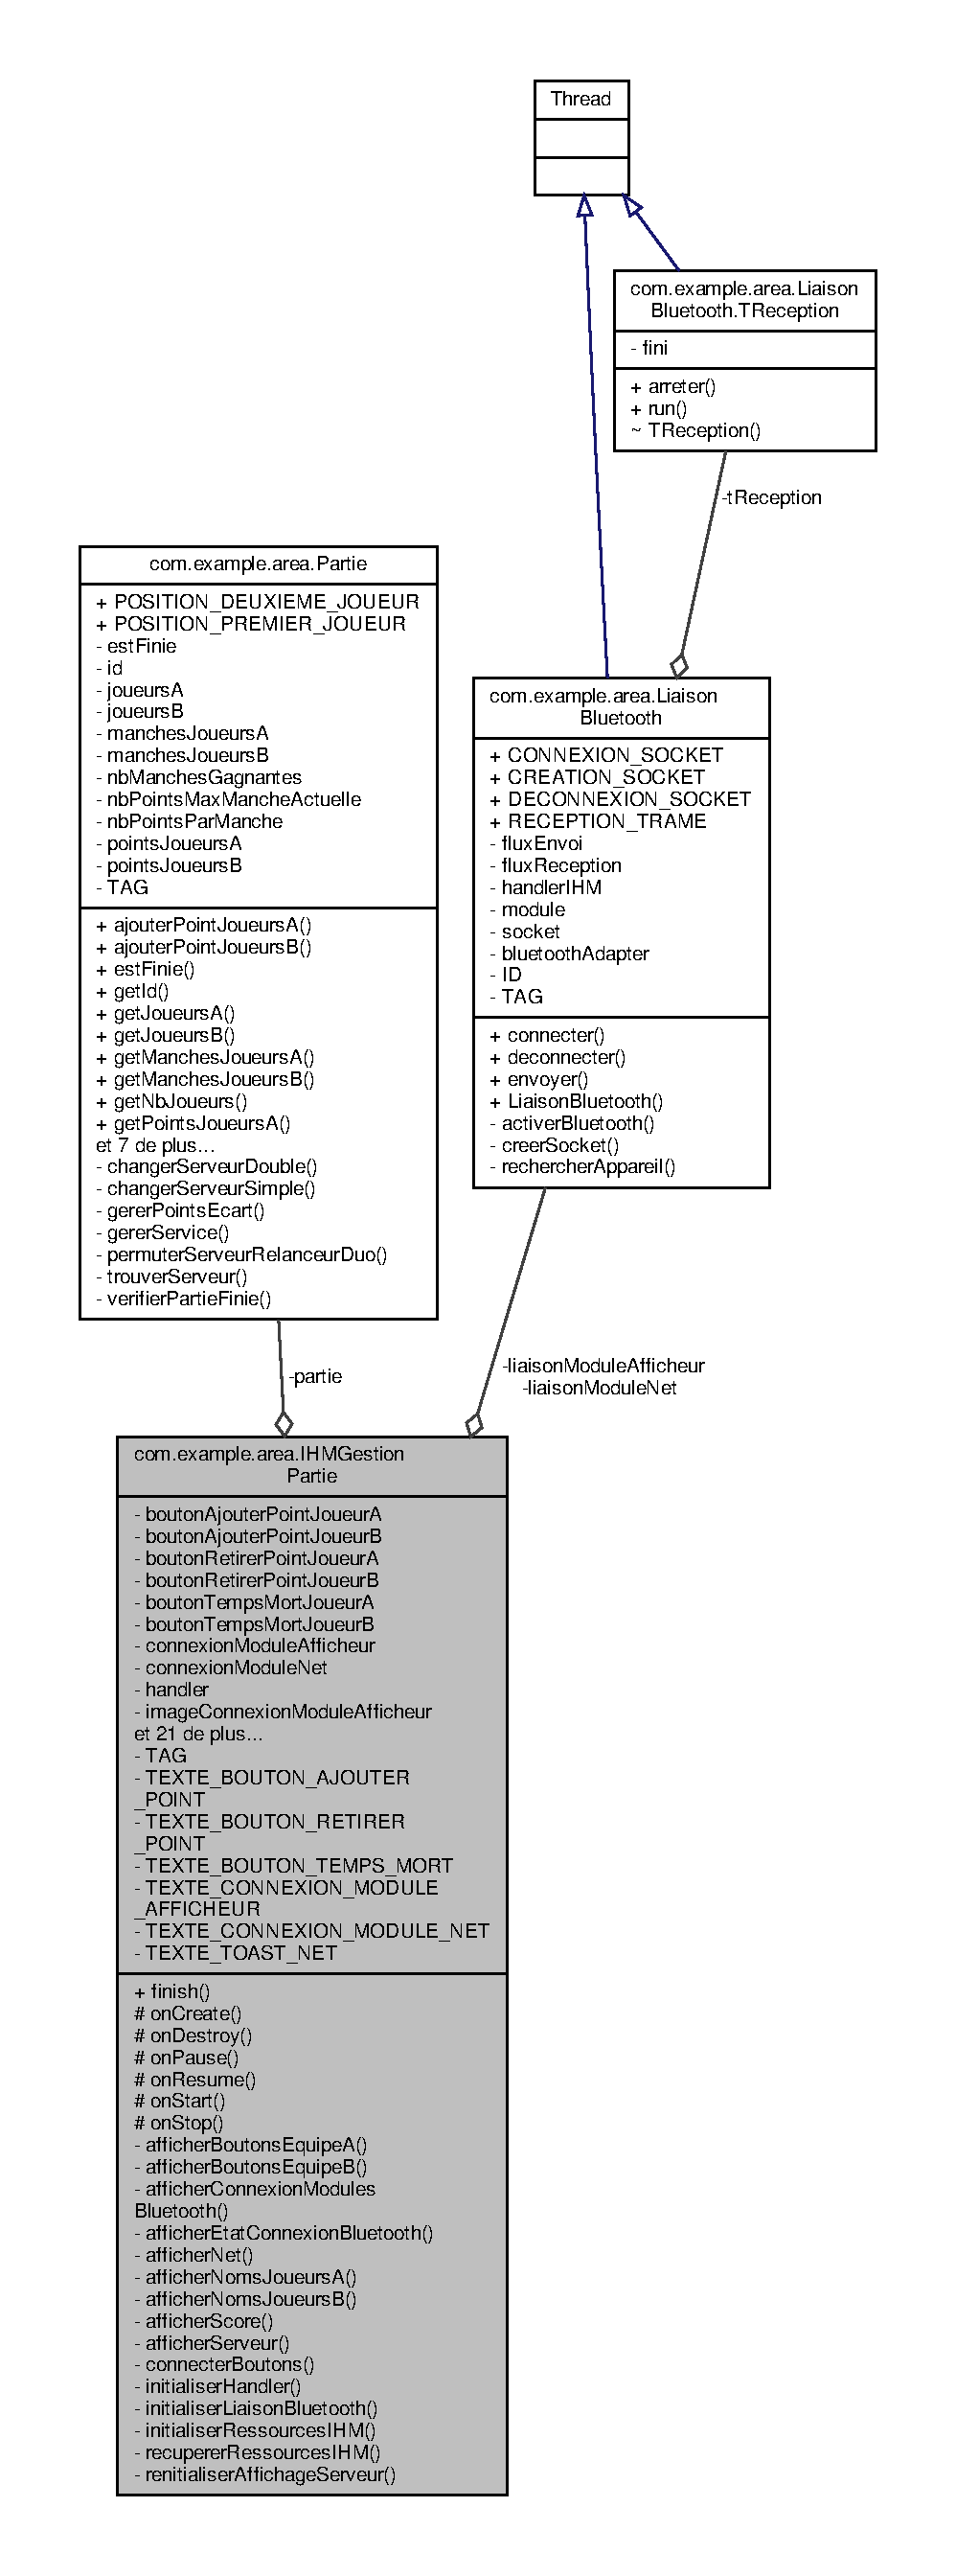
\includegraphics[height=550pt]{classcom_1_1example_1_1area_1_1_i_h_m_gestion_partie__coll__graph}
\end{center}
\end{figure}
\subsubsection*{Fonctions membres publiques}
\begin{DoxyCompactItemize}
\item 
void \hyperlink{classcom_1_1example_1_1area_1_1_i_h_m_gestion_partie_aafa9ce81364dbd851409ae0b38138e28}{finish} ()
\begin{DoxyCompactList}\small\item\em Termine l\textquotesingle{}activité \end{DoxyCompactList}\end{DoxyCompactItemize}
\subsubsection*{Fonctions membres protégées}
\begin{DoxyCompactItemize}
\item 
void \hyperlink{classcom_1_1example_1_1area_1_1_i_h_m_gestion_partie_a501249e0f0625aa3e0784ce5f2b51cd8}{on\+Create} (Bundle saved\+Instance\+State)
\begin{DoxyCompactList}\small\item\em Méthode appelée à la création de l\textquotesingle{}activité \end{DoxyCompactList}\item 
void \hyperlink{classcom_1_1example_1_1area_1_1_i_h_m_gestion_partie_a5706132cc0d20b0c4a67fdc2e9c94a4e}{on\+Destroy} ()
\begin{DoxyCompactList}\small\item\em Méthode appelée à la destruction de l\textquotesingle{}application (après \hyperlink{classcom_1_1example_1_1area_1_1_i_h_m_gestion_partie_a67aa6746480bdba2a5744a2ff8d6c48d}{on\+Stop()} et détruite par le système Android) \end{DoxyCompactList}\item 
void \hyperlink{classcom_1_1example_1_1area_1_1_i_h_m_gestion_partie_a05a8b1eabc376a9d06150eaed696e53e}{on\+Pause} ()
\begin{DoxyCompactList}\small\item\em Méthode appelée après qu\textquotesingle{}une boîte de dialogue s\textquotesingle{}est affichée (on reprend sur un \hyperlink{classcom_1_1example_1_1area_1_1_i_h_m_gestion_partie_a8ebd633d46edcc3218f4b5a5826c0163}{on\+Resume()}) ou avant \hyperlink{classcom_1_1example_1_1area_1_1_i_h_m_gestion_partie_a67aa6746480bdba2a5744a2ff8d6c48d}{on\+Stop()} (activité plus visible) \end{DoxyCompactList}\item 
void \hyperlink{classcom_1_1example_1_1area_1_1_i_h_m_gestion_partie_a8ebd633d46edcc3218f4b5a5826c0163}{on\+Resume} ()
\begin{DoxyCompactList}\small\item\em Méthode appelée après \hyperlink{classcom_1_1example_1_1area_1_1_i_h_m_gestion_partie_a132b61f448998b41a12ef50994350c92}{on\+Start()} ou après \hyperlink{classcom_1_1example_1_1area_1_1_i_h_m_gestion_partie_a05a8b1eabc376a9d06150eaed696e53e}{on\+Pause()} \end{DoxyCompactList}\item 
void \hyperlink{classcom_1_1example_1_1area_1_1_i_h_m_gestion_partie_a132b61f448998b41a12ef50994350c92}{on\+Start} ()
\begin{DoxyCompactList}\small\item\em Méthode appelée au démarrage après le \hyperlink{classcom_1_1example_1_1area_1_1_i_h_m_gestion_partie_a501249e0f0625aa3e0784ce5f2b51cd8}{on\+Create()} ou un restart après un \hyperlink{classcom_1_1example_1_1area_1_1_i_h_m_gestion_partie_a67aa6746480bdba2a5744a2ff8d6c48d}{on\+Stop()} \end{DoxyCompactList}\item 
void \hyperlink{classcom_1_1example_1_1area_1_1_i_h_m_gestion_partie_a67aa6746480bdba2a5744a2ff8d6c48d}{on\+Stop} ()
\begin{DoxyCompactList}\small\item\em Méthode appelée lorsque l\textquotesingle{}activité n\textquotesingle{}est plus visible. \end{DoxyCompactList}\end{DoxyCompactItemize}
\subsubsection*{Fonctions membres privées}
\begin{DoxyCompactItemize}
\item 
void \hyperlink{classcom_1_1example_1_1area_1_1_i_h_m_gestion_partie_a6c63ebbc9822ef53f43468d100ab5677}{afficher\+Boutons\+EquipeA} ()
\begin{DoxyCompactList}\small\item\em Affiche les boutons pour l\textquotesingle{}équipe A. \end{DoxyCompactList}\item 
void \hyperlink{classcom_1_1example_1_1area_1_1_i_h_m_gestion_partie_a00c0111f1b2d4d1161515e2c04ca645c}{afficher\+Boutons\+EquipeB} ()
\begin{DoxyCompactList}\small\item\em Affiche les boutons pour l\textquotesingle{}équipe B. \end{DoxyCompactList}\item 
void \hyperlink{classcom_1_1example_1_1area_1_1_i_h_m_gestion_partie_ade4de81cd6978057a06e16e2e577180c}{afficher\+Connexion\+Modules\+Bluetooth} ()
\begin{DoxyCompactList}\small\item\em Affiche les ressources pour le Bluetooth des modules. \end{DoxyCompactList}\item 
void \hyperlink{classcom_1_1example_1_1area_1_1_i_h_m_gestion_partie_a73fa6d212cf9c5e4dc8fadc96d8d35e9}{afficher\+Etat\+Connexion\+Bluetooth} (String nom\+Module, boolean est\+Connecte)
\begin{DoxyCompactList}\small\item\em Affiche l\textquotesingle{}état de la connexion bluetooth des modules. \end{DoxyCompactList}\item 
void \hyperlink{classcom_1_1example_1_1area_1_1_i_h_m_gestion_partie_a1892c3b33ec5d93514dfa8e30f61204d}{afficher\+Net} ()
\begin{DoxyCompactList}\small\item\em Affiche les ressources pour le N\+ET. \end{DoxyCompactList}\item 
void \hyperlink{classcom_1_1example_1_1area_1_1_i_h_m_gestion_partie_adf3bc699cb45da1f1dea4cb5e16e74f3}{afficher\+Noms\+JoueursA} ()
\begin{DoxyCompactList}\small\item\em Affiche le nom et le prénom des JoueursA. \end{DoxyCompactList}\item 
void \hyperlink{classcom_1_1example_1_1area_1_1_i_h_m_gestion_partie_a55e51d83d01ea0c3c6400f6419edfd06}{afficher\+Noms\+JoueursB} ()
\begin{DoxyCompactList}\small\item\em Affiche le nom et le prénom des JoueursB. \end{DoxyCompactList}\item 
void \hyperlink{classcom_1_1example_1_1area_1_1_i_h_m_gestion_partie_a42cce9ee62fd37d687d4a194328aac70}{afficher\+Score} ()
\begin{DoxyCompactList}\small\item\em Affiche les points et les manches gagnées des joueurs de la partie. \end{DoxyCompactList}\item 
void \hyperlink{classcom_1_1example_1_1area_1_1_i_h_m_gestion_partie_adf8fc8de224da80f542675cbb4c2e364}{afficher\+Serveur} ()
\begin{DoxyCompactList}\small\item\em Affiche une image devant le nom du serveur. \end{DoxyCompactList}\item 
void \hyperlink{classcom_1_1example_1_1area_1_1_i_h_m_gestion_partie_a6be1ce3804251a75cef8d58514645e2c}{connecter\+Boutons} ()
\begin{DoxyCompactList}\small\item\em Définit le comportement des boutons. \end{DoxyCompactList}\item 
void \hyperlink{classcom_1_1example_1_1area_1_1_i_h_m_gestion_partie_a26db1ff779d6ce415ab481dd79295115}{initialiser\+Handler} ()
\begin{DoxyCompactList}\small\item\em Initialise le handler permettant le passage des Messages (trames reçues) entre les classes \hyperlink{classcom_1_1example_1_1area_1_1_liaison_bluetooth}{Liaison\+Bluetooth} et \hyperlink{classcom_1_1example_1_1area_1_1_i_h_m_gestion_partie}{I\+H\+M\+Gestion\+Partie}. \end{DoxyCompactList}\item 
void \hyperlink{classcom_1_1example_1_1area_1_1_i_h_m_gestion_partie_a98f583c39004081b004b854085000256}{initialiser\+Liaison\+Bluetooth} ()
\begin{DoxyCompactList}\small\item\em Initialise la liaison Bluetooth. \end{DoxyCompactList}\item 
void \hyperlink{classcom_1_1example_1_1area_1_1_i_h_m_gestion_partie_a7d67797752c3b0f4e0cab951c8e11e8d}{initialiser\+Ressources\+I\+HM} ()
\begin{DoxyCompactList}\small\item\em Initialise les ressources graphiques de l\textquotesingle{}activité \end{DoxyCompactList}\item 
void \hyperlink{classcom_1_1example_1_1area_1_1_i_h_m_gestion_partie_a2161909470bc787c850df7266c44a0c2}{recuperer\+Ressources\+I\+HM} ()
\begin{DoxyCompactList}\small\item\em Recupère les ressources graphiques de l\textquotesingle{}activité \end{DoxyCompactList}\item 
void \hyperlink{classcom_1_1example_1_1area_1_1_i_h_m_gestion_partie_a4f5930a69896d1d75add34badfb168eb}{renitialiser\+Affichage\+Serveur} ()
\begin{DoxyCompactList}\small\item\em Réinitialise l\textquotesingle{}affichage du serveur. \end{DoxyCompactList}\end{DoxyCompactItemize}
\subsubsection*{Attributs privés}
\begin{DoxyCompactItemize}
\item 
Button \hyperlink{classcom_1_1example_1_1area_1_1_i_h_m_gestion_partie_aa99f420624fb6c990516b30ebe0805cc}{bouton\+Ajouter\+Point\+JoueurA}
\item 
Button \hyperlink{classcom_1_1example_1_1area_1_1_i_h_m_gestion_partie_a8381630a907132144271c11cba2dce20}{bouton\+Ajouter\+Point\+JoueurB}
\item 
Button \hyperlink{classcom_1_1example_1_1area_1_1_i_h_m_gestion_partie_af59fb470e464a16a7f09f4440b18c2e8}{bouton\+Retirer\+Point\+JoueurA}
\item 
Button \hyperlink{classcom_1_1example_1_1area_1_1_i_h_m_gestion_partie_a198ecded9484cec42303eb70246bd590}{bouton\+Retirer\+Point\+JoueurB}
\item 
Button \hyperlink{classcom_1_1example_1_1area_1_1_i_h_m_gestion_partie_a1014526b0dcc0266e184dc2787fbeeef}{bouton\+Temps\+Mort\+JoueurA}
\item 
Button \hyperlink{classcom_1_1example_1_1area_1_1_i_h_m_gestion_partie_a35331b85b4b0acc71a4ede7c78819bc0}{bouton\+Temps\+Mort\+JoueurB}
\item 
Text\+View \hyperlink{classcom_1_1example_1_1area_1_1_i_h_m_gestion_partie_a77e3d7f58799c309694b3ccbb3318150}{connexion\+Module\+Afficheur}
\item 
Text\+View \hyperlink{classcom_1_1example_1_1area_1_1_i_h_m_gestion_partie_a80163f148ea0264b5395a7c55ee5b4ed}{connexion\+Module\+Net}
\item 
Handler \hyperlink{classcom_1_1example_1_1area_1_1_i_h_m_gestion_partie_ace8429e695c3e7d695ba98bf2dcd66f2}{handler} = null
\item 
Image\+View \hyperlink{classcom_1_1example_1_1area_1_1_i_h_m_gestion_partie_aae13761712b67eac1e69ac900c265ffc}{image\+Connexion\+Module\+Afficheur}
\item 
Image\+View \hyperlink{classcom_1_1example_1_1area_1_1_i_h_m_gestion_partie_a98c578b0056e17278e27aacefa933952}{image\+Connexion\+Module\+Net}
\item 
Image\+View \hyperlink{classcom_1_1example_1_1area_1_1_i_h_m_gestion_partie_ad66029deaf2045f16e86ed6059501a1a}{image\+Serveur\+Deuxieme\+JoueurA}
\item 
Image\+View \hyperlink{classcom_1_1example_1_1area_1_1_i_h_m_gestion_partie_a543e5c8605174e111ada0719a0d86fe1}{image\+Serveur\+Deuxieme\+JoueurB}
\item 
Image\+View \hyperlink{classcom_1_1example_1_1area_1_1_i_h_m_gestion_partie_a811fe6ba189ad62350a6e95c3147a1f0}{image\+Serveur\+JoueurA}
\item 
Image\+View \hyperlink{classcom_1_1example_1_1area_1_1_i_h_m_gestion_partie_a0b78d5ef6419187b3b24a2ab7db7dcea}{image\+Serveur\+JoueurB}
\item 
View \hyperlink{classcom_1_1example_1_1area_1_1_i_h_m_gestion_partie_ae9b9e3bd68c744139fe5b2300528beab}{layout\+Net}
\item 
\hyperlink{classcom_1_1example_1_1area_1_1_liaison_bluetooth}{Liaison\+Bluetooth} \hyperlink{classcom_1_1example_1_1area_1_1_i_h_m_gestion_partie_a126a48e2f28ff098e20f0efb4700145f}{liaison\+Module\+Afficheur} = null
\item 
\hyperlink{classcom_1_1example_1_1area_1_1_liaison_bluetooth}{Liaison\+Bluetooth} \hyperlink{classcom_1_1example_1_1area_1_1_i_h_m_gestion_partie_a20e5bc638f1bd45e80bbadca8e8ec28f}{liaison\+Module\+Net} = null
\item 
Text\+View \hyperlink{classcom_1_1example_1_1area_1_1_i_h_m_gestion_partie_ac30dccc72d814c0d1eb36aeb5f5bdc1f}{manches\+JoueurA}
\item 
Text\+View \hyperlink{classcom_1_1example_1_1area_1_1_i_h_m_gestion_partie_ae60c32d48a9fe634358fae66d760a573}{manches\+JoueurB}
\item 
Text\+View \hyperlink{classcom_1_1example_1_1area_1_1_i_h_m_gestion_partie_ac097d7bed4ac981338629a28c0d70c1d}{net}
\item 
Text\+View \hyperlink{classcom_1_1example_1_1area_1_1_i_h_m_gestion_partie_a00dbc2ac1396af550520dd011d8e01cc}{nom\+Deuxieme\+JoueurA}
\item 
Text\+View \hyperlink{classcom_1_1example_1_1area_1_1_i_h_m_gestion_partie_a68aa62c03f3280a8f22d84e1701c1c3e}{nom\+Deuxieme\+JoueurB}
\item 
Text\+View \hyperlink{classcom_1_1example_1_1area_1_1_i_h_m_gestion_partie_ad7ac57a177098fba4ba7ea29a2418f10}{nom\+JoueurA}
\item 
Text\+View \hyperlink{classcom_1_1example_1_1area_1_1_i_h_m_gestion_partie_a5aba0922e5b556ebc91d67793b149f52}{nom\+JoueurB}
\item 
\hyperlink{classcom_1_1example_1_1area_1_1_partie}{Partie} \hyperlink{classcom_1_1example_1_1area_1_1_i_h_m_gestion_partie_a225e150f813f8fa5c632709a57eacc32}{partie} = null
\item 
Text\+View \hyperlink{classcom_1_1example_1_1area_1_1_i_h_m_gestion_partie_affa1414152ba72b6b19e087049e2bda8}{points\+JoueurA}
\item 
Text\+View \hyperlink{classcom_1_1example_1_1area_1_1_i_h_m_gestion_partie_a88e51101924801095d21f65d16b337f3}{points\+JoueurB}
\item 
Text\+View \hyperlink{classcom_1_1example_1_1area_1_1_i_h_m_gestion_partie_af209e9cda709137d8b77170a35b295e0}{prenom\+Deuxieme\+JoueurA}
\item 
Text\+View \hyperlink{classcom_1_1example_1_1area_1_1_i_h_m_gestion_partie_aa5e959a5694b49790434a7d1006f57f3}{prenom\+Deuxieme\+JoueurB}
\item 
Text\+View \hyperlink{classcom_1_1example_1_1area_1_1_i_h_m_gestion_partie_a9a5b0bc9c6f1d865b85bfe789219e16e}{prenom\+JoueurA}
\item 
Text\+View \hyperlink{classcom_1_1example_1_1area_1_1_i_h_m_gestion_partie_aa25eb218f30b28bb0b750c9fa0c1a9af}{prenom\+JoueurB}
\item 
Text\+View \hyperlink{classcom_1_1example_1_1area_1_1_i_h_m_gestion_partie_a84e6684857fc76364978fff7bfbc4e00}{tiret}
\item 
Toast \hyperlink{classcom_1_1example_1_1area_1_1_i_h_m_gestion_partie_a490bd4b5241dfe6a5e709209a939fa2e}{toast\+Net}
\end{DoxyCompactItemize}
\subsubsection*{Attributs privés statiques}
\begin{DoxyCompactItemize}
\item 
static final String \hyperlink{classcom_1_1example_1_1area_1_1_i_h_m_gestion_partie_a78af1eb84e4a48b7f69c3ebee193933c}{T\+AG} = \char`\"{}\+\_\+\+I\+H\+M\+Gestion\+Partie\char`\"{}
\begin{DoxyCompactList}\small\item\em T\+AG pour les logs. \end{DoxyCompactList}\item 
static final String \hyperlink{classcom_1_1example_1_1area_1_1_i_h_m_gestion_partie_a29eb33d17f8f318937bd01705f5769d8}{T\+E\+X\+T\+E\+\_\+\+B\+O\+U\+T\+O\+N\+\_\+\+A\+J\+O\+U\+T\+E\+R\+\_\+\+P\+O\+I\+NT} = \char`\"{}+1\char`\"{}
\item 
static final String \hyperlink{classcom_1_1example_1_1area_1_1_i_h_m_gestion_partie_a9218ba4464b7631738927d74539ac927}{T\+E\+X\+T\+E\+\_\+\+B\+O\+U\+T\+O\+N\+\_\+\+R\+E\+T\+I\+R\+E\+R\+\_\+\+P\+O\+I\+NT} = \char`\"{}-\/1\char`\"{}
\item 
static final String \hyperlink{classcom_1_1example_1_1area_1_1_i_h_m_gestion_partie_abc36e82bb3c4a2fb719305ea9e525c9b}{T\+E\+X\+T\+E\+\_\+\+B\+O\+U\+T\+O\+N\+\_\+\+T\+E\+M\+P\+S\+\_\+\+M\+O\+RT} = \char`\"{}Temps mort\char`\"{}
\item 
static final String \hyperlink{classcom_1_1example_1_1area_1_1_i_h_m_gestion_partie_a60d4b79c44e29fe68c565cf24ed6a22a}{T\+E\+X\+T\+E\+\_\+\+C\+O\+N\+N\+E\+X\+I\+O\+N\+\_\+\+M\+O\+D\+U\+L\+E\+\_\+\+A\+F\+F\+I\+C\+H\+E\+UR} = \char`\"{}Module Afficheur \char`\"{}
\item 
static final String \hyperlink{classcom_1_1example_1_1area_1_1_i_h_m_gestion_partie_a12cdd76d3c9dec83783e40a0d017ac17}{T\+E\+X\+T\+E\+\_\+\+C\+O\+N\+N\+E\+X\+I\+O\+N\+\_\+\+M\+O\+D\+U\+L\+E\+\_\+\+N\+ET} = \char`\"{}Module N\+ET \char`\"{}
\item 
static final String \hyperlink{classcom_1_1example_1_1area_1_1_i_h_m_gestion_partie_aa5b1cdff8bb4d6f6157ae215f43062c5}{T\+E\+X\+T\+E\+\_\+\+T\+O\+A\+S\+T\+\_\+\+N\+ET} = \char`\"{}N\+ET\char`\"{}
\end{DoxyCompactItemize}


\subsubsection{Description détaillée}
L\textquotesingle{}activité de gestion d\textquotesingle{}une partie de l\textquotesingle{}application A\+R\+EA. 

Définition à la ligne \hyperlink{_i_h_m_gestion_partie_8java_source_l00047}{47} du fichier \hyperlink{_i_h_m_gestion_partie_8java_source}{I\+H\+M\+Gestion\+Partie.\+java}.



\subsubsection{Documentation des fonctions membres}
\mbox{\Hypertarget{classcom_1_1example_1_1area_1_1_i_h_m_gestion_partie_a6c63ebbc9822ef53f43468d100ab5677}\label{classcom_1_1example_1_1area_1_1_i_h_m_gestion_partie_a6c63ebbc9822ef53f43468d100ab5677}} 
\index{com\+::example\+::area\+::\+I\+H\+M\+Gestion\+Partie@{com\+::example\+::area\+::\+I\+H\+M\+Gestion\+Partie}!afficher\+Boutons\+EquipeA@{afficher\+Boutons\+EquipeA}}
\index{afficher\+Boutons\+EquipeA@{afficher\+Boutons\+EquipeA}!com\+::example\+::area\+::\+I\+H\+M\+Gestion\+Partie@{com\+::example\+::area\+::\+I\+H\+M\+Gestion\+Partie}}
\paragraph{\texorpdfstring{afficher\+Boutons\+Equipe\+A()}{afficherBoutonsEquipeA()}}
{\footnotesize\ttfamily void com.\+example.\+area.\+I\+H\+M\+Gestion\+Partie.\+afficher\+Boutons\+EquipeA (\begin{DoxyParamCaption}{ }\end{DoxyParamCaption})\hspace{0.3cm}{\ttfamily [private]}}



Affiche les boutons pour l\textquotesingle{}équipe A. 

\begin{DoxyRefDesc}{A faire}
\item[\hyperlink{todo__todo000001}{A faire}]Revoir taille des boutons \char`\"{}-\/1\char`\"{} \end{DoxyRefDesc}


Définition à la ligne \hyperlink{_i_h_m_gestion_partie_8java_source_l00265}{265} du fichier \hyperlink{_i_h_m_gestion_partie_8java_source}{I\+H\+M\+Gestion\+Partie.\+java}.



Référencé par \hyperlink{_i_h_m_gestion_partie_8java_source_l00223}{com.\+example.\+area.\+I\+H\+M\+Gestion\+Partie.\+initialiser\+Ressources\+I\+H\+M()}.


\begin{DoxyCode}
00266     \{
00270         \hyperlink{classcom_1_1example_1_1area_1_1_i_h_m_gestion_partie_aa99f420624fb6c990516b30ebe0805cc}{boutonAjouterPointJoueurA}.setText(
      \hyperlink{classcom_1_1example_1_1area_1_1_i_h_m_gestion_partie_a29eb33d17f8f318937bd01705f5769d8}{TEXTE\_BOUTON\_AJOUTER\_POINT});
00271         \hyperlink{classcom_1_1example_1_1area_1_1_i_h_m_gestion_partie_af59fb470e464a16a7f09f4440b18c2e8}{boutonRetirerPointJoueurA}.setText(
      \hyperlink{classcom_1_1example_1_1area_1_1_i_h_m_gestion_partie_a9218ba4464b7631738927d74539ac927}{TEXTE\_BOUTON\_RETIRER\_POINT});
00272         \hyperlink{classcom_1_1example_1_1area_1_1_i_h_m_gestion_partie_a1014526b0dcc0266e184dc2787fbeeef}{boutonTempsMortJoueurA}.setText(
      \hyperlink{classcom_1_1example_1_1area_1_1_i_h_m_gestion_partie_abc36e82bb3c4a2fb719305ea9e525c9b}{TEXTE\_BOUTON\_TEMPS\_MORT});
00273     \}
\end{DoxyCode}
\mbox{\Hypertarget{classcom_1_1example_1_1area_1_1_i_h_m_gestion_partie_a00c0111f1b2d4d1161515e2c04ca645c}\label{classcom_1_1example_1_1area_1_1_i_h_m_gestion_partie_a00c0111f1b2d4d1161515e2c04ca645c}} 
\index{com\+::example\+::area\+::\+I\+H\+M\+Gestion\+Partie@{com\+::example\+::area\+::\+I\+H\+M\+Gestion\+Partie}!afficher\+Boutons\+EquipeB@{afficher\+Boutons\+EquipeB}}
\index{afficher\+Boutons\+EquipeB@{afficher\+Boutons\+EquipeB}!com\+::example\+::area\+::\+I\+H\+M\+Gestion\+Partie@{com\+::example\+::area\+::\+I\+H\+M\+Gestion\+Partie}}
\paragraph{\texorpdfstring{afficher\+Boutons\+Equipe\+B()}{afficherBoutonsEquipeB()}}
{\footnotesize\ttfamily void com.\+example.\+area.\+I\+H\+M\+Gestion\+Partie.\+afficher\+Boutons\+EquipeB (\begin{DoxyParamCaption}{ }\end{DoxyParamCaption})\hspace{0.3cm}{\ttfamily [private]}}



Affiche les boutons pour l\textquotesingle{}équipe B. 

\begin{DoxyRefDesc}{A faire}
\item[\hyperlink{todo__todo000002}{A faire}]Revoir taille des boutons \char`\"{}-\/1\char`\"{} \end{DoxyRefDesc}


Définition à la ligne \hyperlink{_i_h_m_gestion_partie_8java_source_l00278}{278} du fichier \hyperlink{_i_h_m_gestion_partie_8java_source}{I\+H\+M\+Gestion\+Partie.\+java}.



Référencé par \hyperlink{_i_h_m_gestion_partie_8java_source_l00223}{com.\+example.\+area.\+I\+H\+M\+Gestion\+Partie.\+initialiser\+Ressources\+I\+H\+M()}.


\begin{DoxyCode}
00279     \{
00283         \hyperlink{classcom_1_1example_1_1area_1_1_i_h_m_gestion_partie_a8381630a907132144271c11cba2dce20}{boutonAjouterPointJoueurB}.setText(
      \hyperlink{classcom_1_1example_1_1area_1_1_i_h_m_gestion_partie_a29eb33d17f8f318937bd01705f5769d8}{TEXTE\_BOUTON\_AJOUTER\_POINT});
00284         \hyperlink{classcom_1_1example_1_1area_1_1_i_h_m_gestion_partie_a198ecded9484cec42303eb70246bd590}{boutonRetirerPointJoueurB}.setText(
      \hyperlink{classcom_1_1example_1_1area_1_1_i_h_m_gestion_partie_a9218ba4464b7631738927d74539ac927}{TEXTE\_BOUTON\_RETIRER\_POINT});
00285         \hyperlink{classcom_1_1example_1_1area_1_1_i_h_m_gestion_partie_a35331b85b4b0acc71a4ede7c78819bc0}{boutonTempsMortJoueurB}.setText(
      \hyperlink{classcom_1_1example_1_1area_1_1_i_h_m_gestion_partie_abc36e82bb3c4a2fb719305ea9e525c9b}{TEXTE\_BOUTON\_TEMPS\_MORT});
00286     \}
\end{DoxyCode}
\mbox{\Hypertarget{classcom_1_1example_1_1area_1_1_i_h_m_gestion_partie_ade4de81cd6978057a06e16e2e577180c}\label{classcom_1_1example_1_1area_1_1_i_h_m_gestion_partie_ade4de81cd6978057a06e16e2e577180c}} 
\index{com\+::example\+::area\+::\+I\+H\+M\+Gestion\+Partie@{com\+::example\+::area\+::\+I\+H\+M\+Gestion\+Partie}!afficher\+Connexion\+Modules\+Bluetooth@{afficher\+Connexion\+Modules\+Bluetooth}}
\index{afficher\+Connexion\+Modules\+Bluetooth@{afficher\+Connexion\+Modules\+Bluetooth}!com\+::example\+::area\+::\+I\+H\+M\+Gestion\+Partie@{com\+::example\+::area\+::\+I\+H\+M\+Gestion\+Partie}}
\paragraph{\texorpdfstring{afficher\+Connexion\+Modules\+Bluetooth()}{afficherConnexionModulesBluetooth()}}
{\footnotesize\ttfamily void com.\+example.\+area.\+I\+H\+M\+Gestion\+Partie.\+afficher\+Connexion\+Modules\+Bluetooth (\begin{DoxyParamCaption}{ }\end{DoxyParamCaption})\hspace{0.3cm}{\ttfamily [private]}}



Affiche les ressources pour le Bluetooth des modules. 



Définition à la ligne \hyperlink{_i_h_m_gestion_partie_8java_source_l00242}{242} du fichier \hyperlink{_i_h_m_gestion_partie_8java_source}{I\+H\+M\+Gestion\+Partie.\+java}.



Référencé par \hyperlink{_i_h_m_gestion_partie_8java_source_l00223}{com.\+example.\+area.\+I\+H\+M\+Gestion\+Partie.\+initialiser\+Ressources\+I\+H\+M()}.


\begin{DoxyCode}
00243     \{
00244         \hyperlink{classcom_1_1example_1_1area_1_1_i_h_m_gestion_partie_a98c578b0056e17278e27aacefa933952}{imageConnexionModuleNet}.setColorFilter(Color.RED);
00245         \hyperlink{classcom_1_1example_1_1area_1_1_i_h_m_gestion_partie_a80163f148ea0264b5395a7c55ee5b4ed}{connexionModuleNet}.setText(\hyperlink{classcom_1_1example_1_1area_1_1_i_h_m_gestion_partie_a12cdd76d3c9dec83783e40a0d017ac17}{TEXTE\_CONNEXION\_MODULE\_NET});
00246         \hyperlink{classcom_1_1example_1_1area_1_1_i_h_m_gestion_partie_aae13761712b67eac1e69ac900c265ffc}{imageConnexionModuleAfficheur}.setColorFilter(Color.RED);
00247         \hyperlink{classcom_1_1example_1_1area_1_1_i_h_m_gestion_partie_a77e3d7f58799c309694b3ccbb3318150}{connexionModuleAfficheur}.setText(
      \hyperlink{classcom_1_1example_1_1area_1_1_i_h_m_gestion_partie_a60d4b79c44e29fe68c565cf24ed6a22a}{TEXTE\_CONNEXION\_MODULE\_AFFICHEUR});
00248     \}
\end{DoxyCode}
\mbox{\Hypertarget{classcom_1_1example_1_1area_1_1_i_h_m_gestion_partie_a73fa6d212cf9c5e4dc8fadc96d8d35e9}\label{classcom_1_1example_1_1area_1_1_i_h_m_gestion_partie_a73fa6d212cf9c5e4dc8fadc96d8d35e9}} 
\index{com\+::example\+::area\+::\+I\+H\+M\+Gestion\+Partie@{com\+::example\+::area\+::\+I\+H\+M\+Gestion\+Partie}!afficher\+Etat\+Connexion\+Bluetooth@{afficher\+Etat\+Connexion\+Bluetooth}}
\index{afficher\+Etat\+Connexion\+Bluetooth@{afficher\+Etat\+Connexion\+Bluetooth}!com\+::example\+::area\+::\+I\+H\+M\+Gestion\+Partie@{com\+::example\+::area\+::\+I\+H\+M\+Gestion\+Partie}}
\paragraph{\texorpdfstring{afficher\+Etat\+Connexion\+Bluetooth()}{afficherEtatConnexionBluetooth()}}
{\footnotesize\ttfamily void com.\+example.\+area.\+I\+H\+M\+Gestion\+Partie.\+afficher\+Etat\+Connexion\+Bluetooth (\begin{DoxyParamCaption}\item[{String}]{nom\+Module,  }\item[{boolean}]{est\+Connecte }\end{DoxyParamCaption})\hspace{0.3cm}{\ttfamily [private]}}



Affiche l\textquotesingle{}état de la connexion bluetooth des modules. 


\begin{DoxyParams}{Paramètres}
{\em nom\+Module} & Le nom du module concerné \\
\hline
{\em est\+Connecte} & Représente l\textquotesingle{}état de la connexion du module \\
\hline
\end{DoxyParams}


Définition à la ligne \hyperlink{_i_h_m_gestion_partie_8java_source_l00488}{488} du fichier \hyperlink{_i_h_m_gestion_partie_8java_source}{I\+H\+M\+Gestion\+Partie.\+java}.



Références \hyperlink{_protocol_a_r_e_a_8java_source_l00025}{com.\+example.\+area.\+Protocol\+A\+R\+E\+A.\+N\+O\+M\+\_\+\+M\+O\+D\+U\+L\+E\+\_\+\+N\+ET}.



Référencé par \hyperlink{_i_h_m_gestion_partie_8java_source_l00291}{com.\+example.\+area.\+I\+H\+M\+Gestion\+Partie.\+initialiser\+Handler()}.


\begin{DoxyCode}
00489     \{
00490         \textcolor{keywordflow}{if} (nomModule.startsWith(ProtocolAREA.NOM\_MODULE\_NET))
00491         \{
00492             \hyperlink{classcom_1_1example_1_1area_1_1_i_h_m_gestion_partie_a98c578b0056e17278e27aacefa933952}{imageConnexionModuleNet}.setColorFilter(Color.RED);
00493             \textcolor{keywordflow}{if} (estConnecte)
00494                 \hyperlink{classcom_1_1example_1_1area_1_1_i_h_m_gestion_partie_a98c578b0056e17278e27aacefa933952}{imageConnexionModuleNet}.setColorFilter(Color.GREEN);
00495         \}
00496         \textcolor{keywordflow}{else}
00497         \{
00498             \hyperlink{classcom_1_1example_1_1area_1_1_i_h_m_gestion_partie_aae13761712b67eac1e69ac900c265ffc}{imageConnexionModuleAfficheur}.setColorFilter(Color.RED);
00499             \textcolor{keywordflow}{if} (estConnecte)
00500                 \hyperlink{classcom_1_1example_1_1area_1_1_i_h_m_gestion_partie_aae13761712b67eac1e69ac900c265ffc}{imageConnexionModuleAfficheur}.setColorFilter(Color.GREEN);
00501         \}
00502     \}
\end{DoxyCode}
\mbox{\Hypertarget{classcom_1_1example_1_1area_1_1_i_h_m_gestion_partie_a1892c3b33ec5d93514dfa8e30f61204d}\label{classcom_1_1example_1_1area_1_1_i_h_m_gestion_partie_a1892c3b33ec5d93514dfa8e30f61204d}} 
\index{com\+::example\+::area\+::\+I\+H\+M\+Gestion\+Partie@{com\+::example\+::area\+::\+I\+H\+M\+Gestion\+Partie}!afficher\+Net@{afficher\+Net}}
\index{afficher\+Net@{afficher\+Net}!com\+::example\+::area\+::\+I\+H\+M\+Gestion\+Partie@{com\+::example\+::area\+::\+I\+H\+M\+Gestion\+Partie}}
\paragraph{\texorpdfstring{afficher\+Net()}{afficherNet()}}
{\footnotesize\ttfamily void com.\+example.\+area.\+I\+H\+M\+Gestion\+Partie.\+afficher\+Net (\begin{DoxyParamCaption}{ }\end{DoxyParamCaption})\hspace{0.3cm}{\ttfamily [private]}}



Affiche les ressources pour le N\+ET. 



Définition à la ligne \hyperlink{_i_h_m_gestion_partie_8java_source_l00253}{253} du fichier \hyperlink{_i_h_m_gestion_partie_8java_source}{I\+H\+M\+Gestion\+Partie.\+java}.



Référencé par \hyperlink{_i_h_m_gestion_partie_8java_source_l00223}{com.\+example.\+area.\+I\+H\+M\+Gestion\+Partie.\+initialiser\+Ressources\+I\+H\+M()}.


\begin{DoxyCode}
00254     \{
00255         \hyperlink{classcom_1_1example_1_1area_1_1_i_h_m_gestion_partie_a84e6684857fc76364978fff7bfbc4e00}{tiret}.setText(\textcolor{stringliteral}{"-"});
00256         \hyperlink{classcom_1_1example_1_1area_1_1_i_h_m_gestion_partie_ac097d7bed4ac981338629a28c0d70c1d}{net}.setText(\hyperlink{classcom_1_1example_1_1area_1_1_i_h_m_gestion_partie_aa5b1cdff8bb4d6f6157ae215f43062c5}{TEXTE\_TOAST\_NET});
00257         \hyperlink{classcom_1_1example_1_1area_1_1_i_h_m_gestion_partie_a490bd4b5241dfe6a5e709209a939fa2e}{toastNet}.setDuration(Toast.LENGTH\_LONG);
00258         \hyperlink{classcom_1_1example_1_1area_1_1_i_h_m_gestion_partie_a490bd4b5241dfe6a5e709209a939fa2e}{toastNet}.setGravity(Gravity.TOP, 0, 150);
00259         \hyperlink{classcom_1_1example_1_1area_1_1_i_h_m_gestion_partie_a490bd4b5241dfe6a5e709209a939fa2e}{toastNet}.setView(\hyperlink{classcom_1_1example_1_1area_1_1_i_h_m_gestion_partie_ae9b9e3bd68c744139fe5b2300528beab}{layoutNet});
00260     \}
\end{DoxyCode}
\mbox{\Hypertarget{classcom_1_1example_1_1area_1_1_i_h_m_gestion_partie_adf3bc699cb45da1f1dea4cb5e16e74f3}\label{classcom_1_1example_1_1area_1_1_i_h_m_gestion_partie_adf3bc699cb45da1f1dea4cb5e16e74f3}} 
\index{com\+::example\+::area\+::\+I\+H\+M\+Gestion\+Partie@{com\+::example\+::area\+::\+I\+H\+M\+Gestion\+Partie}!afficher\+Noms\+JoueursA@{afficher\+Noms\+JoueursA}}
\index{afficher\+Noms\+JoueursA@{afficher\+Noms\+JoueursA}!com\+::example\+::area\+::\+I\+H\+M\+Gestion\+Partie@{com\+::example\+::area\+::\+I\+H\+M\+Gestion\+Partie}}
\paragraph{\texorpdfstring{afficher\+Noms\+Joueurs\+A()}{afficherNomsJoueursA()}}
{\footnotesize\ttfamily void com.\+example.\+area.\+I\+H\+M\+Gestion\+Partie.\+afficher\+Noms\+JoueursA (\begin{DoxyParamCaption}{ }\end{DoxyParamCaption})\hspace{0.3cm}{\ttfamily [private]}}



Affiche le nom et le prénom des JoueursA. 



Définition à la ligne \hyperlink{_i_h_m_gestion_partie_8java_source_l00401}{401} du fichier \hyperlink{_i_h_m_gestion_partie_8java_source}{I\+H\+M\+Gestion\+Partie.\+java}.



Références \hyperlink{_partie_8java_source_l00064}{com.\+example.\+area.\+Partie.\+get\+Joueurs\+A()}.



Référencé par \hyperlink{_i_h_m_gestion_partie_8java_source_l00223}{com.\+example.\+area.\+I\+H\+M\+Gestion\+Partie.\+initialiser\+Ressources\+I\+H\+M()}.


\begin{DoxyCode}
00402     \{
00403         Vector<Joueur> joueursA = \hyperlink{classcom_1_1example_1_1area_1_1_i_h_m_gestion_partie_a225e150f813f8fa5c632709a57eacc32}{partie}.\hyperlink{classcom_1_1example_1_1area_1_1_partie_a0f944de317206d9b99f9ffc7146a43ef}{getJoueursA}();
00404 
00405         \hyperlink{classcom_1_1example_1_1area_1_1_i_h_m_gestion_partie_ad7ac57a177098fba4ba7ea29a2418f10}{nomJoueurA}.setText(joueursA.elementAt(0).getNom() + \textcolor{stringliteral}{" "});
00406         \hyperlink{classcom_1_1example_1_1area_1_1_i_h_m_gestion_partie_a9a5b0bc9c6f1d865b85bfe789219e16e}{prenomJoueurA}.setText(joueursA.elementAt(0).getPrenom());
00407 
00408         \textcolor{keywordflow}{if}(joueursA.size() > 1)
00409         \{
00410             \hyperlink{classcom_1_1example_1_1area_1_1_i_h_m_gestion_partie_a00dbc2ac1396af550520dd011d8e01cc}{nomDeuxiemeJoueurA}.setText(joueursA.elementAt(1).getNom() + \textcolor{stringliteral}{" "});
00411             \hyperlink{classcom_1_1example_1_1area_1_1_i_h_m_gestion_partie_af209e9cda709137d8b77170a35b295e0}{prenomDeuxiemeJoueurA}.setText(joueursA.elementAt(1).getPrenom());
00412         \}
00413     \}
\end{DoxyCode}
\mbox{\Hypertarget{classcom_1_1example_1_1area_1_1_i_h_m_gestion_partie_a55e51d83d01ea0c3c6400f6419edfd06}\label{classcom_1_1example_1_1area_1_1_i_h_m_gestion_partie_a55e51d83d01ea0c3c6400f6419edfd06}} 
\index{com\+::example\+::area\+::\+I\+H\+M\+Gestion\+Partie@{com\+::example\+::area\+::\+I\+H\+M\+Gestion\+Partie}!afficher\+Noms\+JoueursB@{afficher\+Noms\+JoueursB}}
\index{afficher\+Noms\+JoueursB@{afficher\+Noms\+JoueursB}!com\+::example\+::area\+::\+I\+H\+M\+Gestion\+Partie@{com\+::example\+::area\+::\+I\+H\+M\+Gestion\+Partie}}
\paragraph{\texorpdfstring{afficher\+Noms\+Joueurs\+B()}{afficherNomsJoueursB()}}
{\footnotesize\ttfamily void com.\+example.\+area.\+I\+H\+M\+Gestion\+Partie.\+afficher\+Noms\+JoueursB (\begin{DoxyParamCaption}{ }\end{DoxyParamCaption})\hspace{0.3cm}{\ttfamily [private]}}



Affiche le nom et le prénom des JoueursB. 



Définition à la ligne \hyperlink{_i_h_m_gestion_partie_8java_source_l00418}{418} du fichier \hyperlink{_i_h_m_gestion_partie_8java_source}{I\+H\+M\+Gestion\+Partie.\+java}.



Références \hyperlink{_partie_8java_source_l00072}{com.\+example.\+area.\+Partie.\+get\+Joueurs\+B()}.



Référencé par \hyperlink{_i_h_m_gestion_partie_8java_source_l00223}{com.\+example.\+area.\+I\+H\+M\+Gestion\+Partie.\+initialiser\+Ressources\+I\+H\+M()}.


\begin{DoxyCode}
00419     \{
00420         Vector<Joueur> joueursB = \hyperlink{classcom_1_1example_1_1area_1_1_i_h_m_gestion_partie_a225e150f813f8fa5c632709a57eacc32}{partie}.\hyperlink{classcom_1_1example_1_1area_1_1_partie_a3c6b981de54d03eeb553919983ee3be8}{getJoueursB}();
00421 
00422         \hyperlink{classcom_1_1example_1_1area_1_1_i_h_m_gestion_partie_a5aba0922e5b556ebc91d67793b149f52}{nomJoueurB}.setText(joueursB.elementAt(0).getNom() + \textcolor{stringliteral}{" "});
00423         \hyperlink{classcom_1_1example_1_1area_1_1_i_h_m_gestion_partie_aa25eb218f30b28bb0b750c9fa0c1a9af}{prenomJoueurB}.setText(joueursB.elementAt(0).getPrenom());
00424 
00425         \textcolor{keywordflow}{if}(joueursB.size() > 1)
00426         \{
00427             \hyperlink{classcom_1_1example_1_1area_1_1_i_h_m_gestion_partie_a68aa62c03f3280a8f22d84e1701c1c3e}{nomDeuxiemeJoueurB}.setText(joueursB.elementAt(1).getNom() + \textcolor{stringliteral}{" "});
00428             \hyperlink{classcom_1_1example_1_1area_1_1_i_h_m_gestion_partie_aa5e959a5694b49790434a7d1006f57f3}{prenomDeuxiemeJoueurB}.setText(joueursB.elementAt(1).getPrenom());
00429         \}
00430     \}
\end{DoxyCode}
\mbox{\Hypertarget{classcom_1_1example_1_1area_1_1_i_h_m_gestion_partie_a42cce9ee62fd37d687d4a194328aac70}\label{classcom_1_1example_1_1area_1_1_i_h_m_gestion_partie_a42cce9ee62fd37d687d4a194328aac70}} 
\index{com\+::example\+::area\+::\+I\+H\+M\+Gestion\+Partie@{com\+::example\+::area\+::\+I\+H\+M\+Gestion\+Partie}!afficher\+Score@{afficher\+Score}}
\index{afficher\+Score@{afficher\+Score}!com\+::example\+::area\+::\+I\+H\+M\+Gestion\+Partie@{com\+::example\+::area\+::\+I\+H\+M\+Gestion\+Partie}}
\paragraph{\texorpdfstring{afficher\+Score()}{afficherScore()}}
{\footnotesize\ttfamily void com.\+example.\+area.\+I\+H\+M\+Gestion\+Partie.\+afficher\+Score (\begin{DoxyParamCaption}{ }\end{DoxyParamCaption})\hspace{0.3cm}{\ttfamily [private]}}



Affiche les points et les manches gagnées des joueurs de la partie. 



Définition à la ligne \hyperlink{_i_h_m_gestion_partie_8java_source_l00435}{435} du fichier \hyperlink{_i_h_m_gestion_partie_8java_source}{I\+H\+M\+Gestion\+Partie.\+java}.



Références \hyperlink{_partie_8java_source_l00096}{com.\+example.\+area.\+Partie.\+get\+Manches\+Joueurs\+A()}, \hyperlink{_partie_8java_source_l00104}{com.\+example.\+area.\+Partie.\+get\+Manches\+Joueurs\+B()}, \hyperlink{_partie_8java_source_l00080}{com.\+example.\+area.\+Partie.\+get\+Points\+Joueurs\+A()}, et \hyperlink{_partie_8java_source_l00088}{com.\+example.\+area.\+Partie.\+get\+Points\+Joueurs\+B()}.



Référencé par \hyperlink{_i_h_m_gestion_partie_8java_source_l00346}{com.\+example.\+area.\+I\+H\+M\+Gestion\+Partie.\+connecter\+Boutons()}, et \hyperlink{_i_h_m_gestion_partie_8java_source_l00223}{com.\+example.\+area.\+I\+H\+M\+Gestion\+Partie.\+initialiser\+Ressources\+I\+H\+M()}.


\begin{DoxyCode}
00436     \{
00437         \hyperlink{classcom_1_1example_1_1area_1_1_i_h_m_gestion_partie_affa1414152ba72b6b19e087049e2bda8}{pointsJoueurA}.setText(Integer.toString(\hyperlink{classcom_1_1example_1_1area_1_1_i_h_m_gestion_partie_a225e150f813f8fa5c632709a57eacc32}{partie}.
      \hyperlink{classcom_1_1example_1_1area_1_1_partie_a5ec15306fc24648c1698ea0cdd50bf53}{getPointsJoueursA}()));
00438         \hyperlink{classcom_1_1example_1_1area_1_1_i_h_m_gestion_partie_ac30dccc72d814c0d1eb36aeb5f5bdc1f}{manchesJoueurA}.setText(Integer.toString(\hyperlink{classcom_1_1example_1_1area_1_1_i_h_m_gestion_partie_a225e150f813f8fa5c632709a57eacc32}{partie}.
      \hyperlink{classcom_1_1example_1_1area_1_1_partie_a7c863edbbdd07ddc7f71616949823201}{getManchesJoueursA}()));
00439 
00440         \hyperlink{classcom_1_1example_1_1area_1_1_i_h_m_gestion_partie_a88e51101924801095d21f65d16b337f3}{pointsJoueurB}.setText(Integer.toString(\hyperlink{classcom_1_1example_1_1area_1_1_i_h_m_gestion_partie_a225e150f813f8fa5c632709a57eacc32}{partie}.
      \hyperlink{classcom_1_1example_1_1area_1_1_partie_a376bb79a67c311e1eb681387e9440bbd}{getPointsJoueursB}()));
00441         \hyperlink{classcom_1_1example_1_1area_1_1_i_h_m_gestion_partie_ae60c32d48a9fe634358fae66d760a573}{manchesJoueurB}.setText(Integer.toString(\hyperlink{classcom_1_1example_1_1area_1_1_i_h_m_gestion_partie_a225e150f813f8fa5c632709a57eacc32}{partie}.
      \hyperlink{classcom_1_1example_1_1area_1_1_partie_a706fa101c4fcad9f2ea6473b5778b55e}{getManchesJoueursB}()));
00442     \}
\end{DoxyCode}
\mbox{\Hypertarget{classcom_1_1example_1_1area_1_1_i_h_m_gestion_partie_adf8fc8de224da80f542675cbb4c2e364}\label{classcom_1_1example_1_1area_1_1_i_h_m_gestion_partie_adf8fc8de224da80f542675cbb4c2e364}} 
\index{com\+::example\+::area\+::\+I\+H\+M\+Gestion\+Partie@{com\+::example\+::area\+::\+I\+H\+M\+Gestion\+Partie}!afficher\+Serveur@{afficher\+Serveur}}
\index{afficher\+Serveur@{afficher\+Serveur}!com\+::example\+::area\+::\+I\+H\+M\+Gestion\+Partie@{com\+::example\+::area\+::\+I\+H\+M\+Gestion\+Partie}}
\paragraph{\texorpdfstring{afficher\+Serveur()}{afficherServeur()}}
{\footnotesize\ttfamily void com.\+example.\+area.\+I\+H\+M\+Gestion\+Partie.\+afficher\+Serveur (\begin{DoxyParamCaption}{ }\end{DoxyParamCaption})\hspace{0.3cm}{\ttfamily [private]}}



Affiche une image devant le nom du serveur. 



Définition à la ligne \hyperlink{_i_h_m_gestion_partie_8java_source_l00447}{447} du fichier \hyperlink{_i_h_m_gestion_partie_8java_source}{I\+H\+M\+Gestion\+Partie.\+java}.



Références \hyperlink{_partie_8java_source_l00064}{com.\+example.\+area.\+Partie.\+get\+Joueurs\+A()}, \hyperlink{_joueur_8java_source_l00039}{com.\+example.\+area.\+Joueur.\+get\+Nom()}, \hyperlink{_joueur_8java_source_l00047}{com.\+example.\+area.\+Joueur.\+get\+Prenom()}, \hyperlink{_partie_8java_source_l00334}{com.\+example.\+area.\+Partie.\+get\+Serveur()}, et \hyperlink{_i_h_m_gestion_partie_8java_source_l00475}{com.\+example.\+area.\+I\+H\+M\+Gestion\+Partie.\+renitialiser\+Affichage\+Serveur()}.



Référencé par \hyperlink{_i_h_m_gestion_partie_8java_source_l00346}{com.\+example.\+area.\+I\+H\+M\+Gestion\+Partie.\+connecter\+Boutons()}, et \hyperlink{_i_h_m_gestion_partie_8java_source_l00223}{com.\+example.\+area.\+I\+H\+M\+Gestion\+Partie.\+initialiser\+Ressources\+I\+H\+M()}.


\begin{DoxyCode}
00448     \{
00449          Joueur serveur = \hyperlink{classcom_1_1example_1_1area_1_1_i_h_m_gestion_partie_a225e150f813f8fa5c632709a57eacc32}{partie}.\hyperlink{classcom_1_1example_1_1area_1_1_partie_a34f75da57f51b710fccbce4aafda28d4}{getServeur}();
00450          Vector<Joueur> joueursA = \hyperlink{classcom_1_1example_1_1area_1_1_i_h_m_gestion_partie_a225e150f813f8fa5c632709a57eacc32}{partie}.\hyperlink{classcom_1_1example_1_1area_1_1_partie_a0f944de317206d9b99f9ffc7146a43ef}{getJoueursA}();
00451          \textcolor{keywordtype}{int} indexServeur = joueursA.indexOf(serveur);
00452          String nomCompletServeur = serveur.getNom() + \textcolor{stringliteral}{" "} + serveur.getPrenom();
00453 
00454         \hyperlink{classcom_1_1example_1_1area_1_1_i_h_m_gestion_partie_a4f5930a69896d1d75add34badfb168eb}{renitialiserAffichageServeur}();
00455 
00456         \textcolor{keywordflow}{if}(indexServeur != -1)
00457          \{
00458             \textcolor{keywordflow}{if} (nomCompletServeur.equals((String)\hyperlink{classcom_1_1example_1_1area_1_1_i_h_m_gestion_partie_ad7ac57a177098fba4ba7ea29a2418f10}{nomJoueurA}.getText()+
      \hyperlink{classcom_1_1example_1_1area_1_1_i_h_m_gestion_partie_a9a5b0bc9c6f1d865b85bfe789219e16e}{prenomJoueurA}.getText()))
00459                 \hyperlink{classcom_1_1example_1_1area_1_1_i_h_m_gestion_partie_a811fe6ba189ad62350a6e95c3147a1f0}{imageServeurJoueurA}.setVisibility(View.VISIBLE);
00460             \textcolor{keywordflow}{else}
00461                 \hyperlink{classcom_1_1example_1_1area_1_1_i_h_m_gestion_partie_ad66029deaf2045f16e86ed6059501a1a}{imageServeurDeuxiemeJoueurA}.setVisibility(View.VISIBLE);
00462          \}
00463          \textcolor{keywordflow}{else}
00464          \{
00465              \textcolor{keywordflow}{if} (nomCompletServeur.equals((String)\hyperlink{classcom_1_1example_1_1area_1_1_i_h_m_gestion_partie_a5aba0922e5b556ebc91d67793b149f52}{nomJoueurB}.getText()+
      \hyperlink{classcom_1_1example_1_1area_1_1_i_h_m_gestion_partie_aa25eb218f30b28bb0b750c9fa0c1a9af}{prenomJoueurB}.getText()))
00466                  \hyperlink{classcom_1_1example_1_1area_1_1_i_h_m_gestion_partie_a0b78d5ef6419187b3b24a2ab7db7dcea}{imageServeurJoueurB}.setVisibility(View.VISIBLE);
00467              \textcolor{keywordflow}{else}
00468                  \hyperlink{classcom_1_1example_1_1area_1_1_i_h_m_gestion_partie_a543e5c8605174e111ada0719a0d86fe1}{imageServeurDeuxiemeJoueurB}.setVisibility(View.VISIBLE);
00469          \}
00470     \}
\end{DoxyCode}
\mbox{\Hypertarget{classcom_1_1example_1_1area_1_1_i_h_m_gestion_partie_a6be1ce3804251a75cef8d58514645e2c}\label{classcom_1_1example_1_1area_1_1_i_h_m_gestion_partie_a6be1ce3804251a75cef8d58514645e2c}} 
\index{com\+::example\+::area\+::\+I\+H\+M\+Gestion\+Partie@{com\+::example\+::area\+::\+I\+H\+M\+Gestion\+Partie}!connecter\+Boutons@{connecter\+Boutons}}
\index{connecter\+Boutons@{connecter\+Boutons}!com\+::example\+::area\+::\+I\+H\+M\+Gestion\+Partie@{com\+::example\+::area\+::\+I\+H\+M\+Gestion\+Partie}}
\paragraph{\texorpdfstring{connecter\+Boutons()}{connecterBoutons()}}
{\footnotesize\ttfamily void com.\+example.\+area.\+I\+H\+M\+Gestion\+Partie.\+connecter\+Boutons (\begin{DoxyParamCaption}{ }\end{DoxyParamCaption})\hspace{0.3cm}{\ttfamily [private]}}



Définit le comportement des boutons. 

\begin{DoxyRefDesc}{A faire}
\item[\hyperlink{todo__todo000004}{A faire}]Gérer la fin d\textquotesingle{}une partie \end{DoxyRefDesc}


Définition à la ligne \hyperlink{_i_h_m_gestion_partie_8java_source_l00346}{346} du fichier \hyperlink{_i_h_m_gestion_partie_8java_source}{I\+H\+M\+Gestion\+Partie.\+java}.



Références \hyperlink{_i_h_m_gestion_partie_8java_source_l00435}{com.\+example.\+area.\+I\+H\+M\+Gestion\+Partie.\+afficher\+Score()}, \hyperlink{_i_h_m_gestion_partie_8java_source_l00447}{com.\+example.\+area.\+I\+H\+M\+Gestion\+Partie.\+afficher\+Serveur()}, \hyperlink{_partie_8java_source_l00128}{com.\+example.\+area.\+Partie.\+ajouter\+Point\+Joueurs\+A()}, \hyperlink{_partie_8java_source_l00147}{com.\+example.\+area.\+Partie.\+ajouter\+Point\+Joueurs\+B()}, \hyperlink{_liaison_bluetooth_8java_source_l00202}{com.\+example.\+area.\+Liaison\+Bluetooth.\+envoyer()}, \hyperlink{_protocol_a_r_e_a_8java_source_l00048}{com.\+example.\+area.\+Protocol\+A\+R\+E\+A.\+fabriquer\+Trame\+Afficheur()}, \hyperlink{_partie_8java_source_l00166}{com.\+example.\+area.\+Partie.\+retirer\+Point\+Joueurs\+A()}, \hyperlink{_partie_8java_source_l00179}{com.\+example.\+area.\+Partie.\+retirer\+Point\+Joueurs\+B()}, \hyperlink{_protocol_a_r_e_a_8java_source_l00037}{com.\+example.\+area.\+Protocol\+A\+R\+E\+A.\+T\+R\+A\+M\+E\+\_\+\+A\+F\+F\+I\+C\+H\+E\+U\+R\+\_\+\+S\+C\+O\+RE}, et \hyperlink{_protocol_a_r_e_a_8java_source_l00033}{com.\+example.\+area.\+Protocol\+A\+R\+E\+A.\+T\+R\+A\+M\+E\+\_\+\+S\+E\+R\+V\+I\+CE}.



Référencé par \hyperlink{_i_h_m_gestion_partie_8java_source_l00106}{com.\+example.\+area.\+I\+H\+M\+Gestion\+Partie.\+on\+Create()}.


\begin{DoxyCode}
00347     \{
00351         \hyperlink{classcom_1_1example_1_1area_1_1_i_h_m_gestion_partie_aa99f420624fb6c990516b30ebe0805cc}{boutonAjouterPointJoueurA}.setOnClickListener(\textcolor{keyword}{new} View.OnClickListener()
00352         \{
00353             \textcolor{keyword}{public} \textcolor{keywordtype}{void} onClick(View v)
00354             \{
00355                 \hyperlink{classcom_1_1example_1_1area_1_1_i_h_m_gestion_partie_a225e150f813f8fa5c632709a57eacc32}{partie}.\hyperlink{classcom_1_1example_1_1area_1_1_partie_abb040a8be4a92a91afded80991d07087}{ajouterPointJoueursA}();
00356                 \hyperlink{classcom_1_1example_1_1area_1_1_i_h_m_gestion_partie_a42cce9ee62fd37d687d4a194328aac70}{afficherScore}();
00357                 \hyperlink{classcom_1_1example_1_1area_1_1_i_h_m_gestion_partie_adf8fc8de224da80f542675cbb4c2e364}{afficherServeur}();
00358                 \hyperlink{classcom_1_1example_1_1area_1_1_i_h_m_gestion_partie_a20e5bc638f1bd45e80bbadca8e8ec28f}{liaisonModuleNet}.\hyperlink{classcom_1_1example_1_1area_1_1_liaison_bluetooth_a67360b2f673b47b8a552a9e789a93fce}{envoyer}(ProtocolAREA.TRAME\_SERVICE);
00359                 \hyperlink{classcom_1_1example_1_1area_1_1_i_h_m_gestion_partie_a126a48e2f28ff098e20f0efb4700145f}{liaisonModuleAfficheur}.\hyperlink{classcom_1_1example_1_1area_1_1_liaison_bluetooth_a67360b2f673b47b8a552a9e789a93fce}{envoyer}(ProtocolAREA.
      fabriquerTrameAfficheur(ProtocolAREA.TRAME\_AFFICHEUR\_SCORE, \hyperlink{classcom_1_1example_1_1area_1_1_i_h_m_gestion_partie_a225e150f813f8fa5c632709a57eacc32}{partie}));
00360             \}
00361         \});
00362 
00363         \hyperlink{classcom_1_1example_1_1area_1_1_i_h_m_gestion_partie_a8381630a907132144271c11cba2dce20}{boutonAjouterPointJoueurB}.setOnClickListener(\textcolor{keyword}{new} View.OnClickListener()
00364         \{
00365             \textcolor{keyword}{public} \textcolor{keywordtype}{void} onClick(View v)
00366             \{
00367                 \hyperlink{classcom_1_1example_1_1area_1_1_i_h_m_gestion_partie_a225e150f813f8fa5c632709a57eacc32}{partie}.\hyperlink{classcom_1_1example_1_1area_1_1_partie_aadc82cc11b982008b81f886adbc4e63a}{ajouterPointJoueursB}();
00368                 \hyperlink{classcom_1_1example_1_1area_1_1_i_h_m_gestion_partie_a42cce9ee62fd37d687d4a194328aac70}{afficherScore}();
00369                 \hyperlink{classcom_1_1example_1_1area_1_1_i_h_m_gestion_partie_adf8fc8de224da80f542675cbb4c2e364}{afficherServeur}();
00370                 \hyperlink{classcom_1_1example_1_1area_1_1_i_h_m_gestion_partie_a20e5bc638f1bd45e80bbadca8e8ec28f}{liaisonModuleNet}.\hyperlink{classcom_1_1example_1_1area_1_1_liaison_bluetooth_a67360b2f673b47b8a552a9e789a93fce}{envoyer}(ProtocolAREA.TRAME\_SERVICE);
00371                 \hyperlink{classcom_1_1example_1_1area_1_1_i_h_m_gestion_partie_a126a48e2f28ff098e20f0efb4700145f}{liaisonModuleAfficheur}.\hyperlink{classcom_1_1example_1_1area_1_1_liaison_bluetooth_a67360b2f673b47b8a552a9e789a93fce}{envoyer}(ProtocolAREA.
      fabriquerTrameAfficheur(ProtocolAREA.TRAME\_AFFICHEUR\_SCORE, \hyperlink{classcom_1_1example_1_1area_1_1_i_h_m_gestion_partie_a225e150f813f8fa5c632709a57eacc32}{partie}));
00372             \}
00373         \});
00374 
00375         \hyperlink{classcom_1_1example_1_1area_1_1_i_h_m_gestion_partie_af59fb470e464a16a7f09f4440b18c2e8}{boutonRetirerPointJoueurA}.setOnClickListener(\textcolor{keyword}{new} View.OnClickListener()
00376         \{
00377             \textcolor{keyword}{public} \textcolor{keywordtype}{void} onClick(View v)
00378             \{
00379                 \hyperlink{classcom_1_1example_1_1area_1_1_i_h_m_gestion_partie_a225e150f813f8fa5c632709a57eacc32}{partie}.\hyperlink{classcom_1_1example_1_1area_1_1_partie_a2847b07aff035a02c130f6219efc5312}{retirerPointJoueursA}();
00380                 \hyperlink{classcom_1_1example_1_1area_1_1_i_h_m_gestion_partie_a42cce9ee62fd37d687d4a194328aac70}{afficherScore}();
00381                 \hyperlink{classcom_1_1example_1_1area_1_1_i_h_m_gestion_partie_adf8fc8de224da80f542675cbb4c2e364}{afficherServeur}();
00382                 \hyperlink{classcom_1_1example_1_1area_1_1_i_h_m_gestion_partie_a126a48e2f28ff098e20f0efb4700145f}{liaisonModuleAfficheur}.\hyperlink{classcom_1_1example_1_1area_1_1_liaison_bluetooth_a67360b2f673b47b8a552a9e789a93fce}{envoyer}(ProtocolAREA.
      fabriquerTrameAfficheur(ProtocolAREA.TRAME\_AFFICHEUR\_SCORE, \hyperlink{classcom_1_1example_1_1area_1_1_i_h_m_gestion_partie_a225e150f813f8fa5c632709a57eacc32}{partie}));
00383             \}
00384         \});
00385 
00386         \hyperlink{classcom_1_1example_1_1area_1_1_i_h_m_gestion_partie_a198ecded9484cec42303eb70246bd590}{boutonRetirerPointJoueurB}.setOnClickListener(\textcolor{keyword}{new} View.OnClickListener()
00387         \{
00388             \textcolor{keyword}{public} \textcolor{keywordtype}{void} onClick(View v)
00389             \{
00390                 \hyperlink{classcom_1_1example_1_1area_1_1_i_h_m_gestion_partie_a225e150f813f8fa5c632709a57eacc32}{partie}.\hyperlink{classcom_1_1example_1_1area_1_1_partie_aa3f7d2c68dcf31a2e48f95c5db9c5663}{retirerPointJoueursB}();
00391                 \hyperlink{classcom_1_1example_1_1area_1_1_i_h_m_gestion_partie_a42cce9ee62fd37d687d4a194328aac70}{afficherScore}();
00392                 \hyperlink{classcom_1_1example_1_1area_1_1_i_h_m_gestion_partie_adf8fc8de224da80f542675cbb4c2e364}{afficherServeur}();
00393                 \hyperlink{classcom_1_1example_1_1area_1_1_i_h_m_gestion_partie_a126a48e2f28ff098e20f0efb4700145f}{liaisonModuleAfficheur}.\hyperlink{classcom_1_1example_1_1area_1_1_liaison_bluetooth_a67360b2f673b47b8a552a9e789a93fce}{envoyer}(ProtocolAREA.
      fabriquerTrameAfficheur(ProtocolAREA.TRAME\_AFFICHEUR\_SCORE, \hyperlink{classcom_1_1example_1_1area_1_1_i_h_m_gestion_partie_a225e150f813f8fa5c632709a57eacc32}{partie}));
00394             \}
00395         \});
00396     \}
\end{DoxyCode}
\mbox{\Hypertarget{classcom_1_1example_1_1area_1_1_i_h_m_gestion_partie_aafa9ce81364dbd851409ae0b38138e28}\label{classcom_1_1example_1_1area_1_1_i_h_m_gestion_partie_aafa9ce81364dbd851409ae0b38138e28}} 
\index{com\+::example\+::area\+::\+I\+H\+M\+Gestion\+Partie@{com\+::example\+::area\+::\+I\+H\+M\+Gestion\+Partie}!finish@{finish}}
\index{finish@{finish}!com\+::example\+::area\+::\+I\+H\+M\+Gestion\+Partie@{com\+::example\+::area\+::\+I\+H\+M\+Gestion\+Partie}}
\paragraph{\texorpdfstring{finish()}{finish()}}
{\footnotesize\ttfamily void com.\+example.\+area.\+I\+H\+M\+Gestion\+Partie.\+finish (\begin{DoxyParamCaption}{ }\end{DoxyParamCaption})}



Termine l\textquotesingle{}activité 

\begin{DoxyRefDesc}{A faire}
\item[\hyperlink{todo__todo000005}{A faire}]Gérer le retour d\textquotesingle{}une partie \end{DoxyRefDesc}


Définition à la ligne \hyperlink{_i_h_m_gestion_partie_8java_source_l00508}{508} du fichier \hyperlink{_i_h_m_gestion_partie_8java_source}{I\+H\+M\+Gestion\+Partie.\+java}.


\begin{DoxyCode}
00509     \{
00510         Log.d(\hyperlink{classcom_1_1example_1_1area_1_1_i_h_m_gestion_partie_a78af1eb84e4a48b7f69c3ebee193933c}{TAG}, \textcolor{stringliteral}{"finish()"});
00511 
00512         Intent intent = \textcolor{keyword}{new} Intent();
00516         \textcolor{comment}{// cf. intent.putExtra()}
00517 
00518         setResult(RESULT\_OK, intent);
00519         super.finish();
00520     \}
\end{DoxyCode}
\mbox{\Hypertarget{classcom_1_1example_1_1area_1_1_i_h_m_gestion_partie_a26db1ff779d6ce415ab481dd79295115}\label{classcom_1_1example_1_1area_1_1_i_h_m_gestion_partie_a26db1ff779d6ce415ab481dd79295115}} 
\index{com\+::example\+::area\+::\+I\+H\+M\+Gestion\+Partie@{com\+::example\+::area\+::\+I\+H\+M\+Gestion\+Partie}!initialiser\+Handler@{initialiser\+Handler}}
\index{initialiser\+Handler@{initialiser\+Handler}!com\+::example\+::area\+::\+I\+H\+M\+Gestion\+Partie@{com\+::example\+::area\+::\+I\+H\+M\+Gestion\+Partie}}
\paragraph{\texorpdfstring{initialiser\+Handler()}{initialiserHandler()}}
{\footnotesize\ttfamily void com.\+example.\+area.\+I\+H\+M\+Gestion\+Partie.\+initialiser\+Handler (\begin{DoxyParamCaption}{ }\end{DoxyParamCaption})\hspace{0.3cm}{\ttfamily [private]}}



Initialise le handler permettant le passage des Messages (trames reçues) entre les classes \hyperlink{classcom_1_1example_1_1area_1_1_liaison_bluetooth}{Liaison\+Bluetooth} et \hyperlink{classcom_1_1example_1_1area_1_1_i_h_m_gestion_partie}{I\+H\+M\+Gestion\+Partie}. 



Définition à la ligne \hyperlink{_i_h_m_gestion_partie_8java_source_l00291}{291} du fichier \hyperlink{_i_h_m_gestion_partie_8java_source}{I\+H\+M\+Gestion\+Partie.\+java}.



Références \hyperlink{_i_h_m_gestion_partie_8java_source_l00488}{com.\+example.\+area.\+I\+H\+M\+Gestion\+Partie.\+afficher\+Etat\+Connexion\+Bluetooth()}, \hyperlink{_liaison_bluetooth_8java_source_l00036}{com.\+example.\+area.\+Liaison\+Bluetooth.\+C\+O\+N\+N\+E\+X\+I\+O\+N\+\_\+\+S\+O\+C\+K\+ET}, \hyperlink{_liaison_bluetooth_8java_source_l00035}{com.\+example.\+area.\+Liaison\+Bluetooth.\+C\+R\+E\+A\+T\+I\+O\+N\+\_\+\+S\+O\+C\+K\+ET}, \hyperlink{_liaison_bluetooth_8java_source_l00037}{com.\+example.\+area.\+Liaison\+Bluetooth.\+D\+E\+C\+O\+N\+N\+E\+X\+I\+O\+N\+\_\+\+S\+O\+C\+K\+ET}, \hyperlink{_liaison_bluetooth_8java_source_l00202}{com.\+example.\+area.\+Liaison\+Bluetooth.\+envoyer()}, \hyperlink{_protocol_a_r_e_a_8java_source_l00048}{com.\+example.\+area.\+Protocol\+A\+R\+E\+A.\+fabriquer\+Trame\+Afficheur()}, \hyperlink{_liaison_bluetooth_8java_source_l00038}{com.\+example.\+area.\+Liaison\+Bluetooth.\+R\+E\+C\+E\+P\+T\+I\+O\+N\+\_\+\+T\+R\+A\+ME}, \hyperlink{_protocol_a_r_e_a_8java_source_l00039}{com.\+example.\+area.\+Protocol\+A\+R\+E\+A.\+T\+R\+A\+M\+E\+\_\+\+A\+F\+F\+I\+C\+H\+E\+U\+R\+\_\+\+N\+ET}, et \hyperlink{_protocol_a_r_e_a_8java_source_l00117}{com.\+example.\+area.\+Protocol\+A\+R\+E\+A.\+verifier\+Trame\+Net()}.



Référencé par \hyperlink{_i_h_m_gestion_partie_8java_source_l00106}{com.\+example.\+area.\+I\+H\+M\+Gestion\+Partie.\+on\+Create()}.


\begin{DoxyCode}
00292     \{
00293         this.\hyperlink{classcom_1_1example_1_1area_1_1_i_h_m_gestion_partie_ace8429e695c3e7d695ba98bf2dcd66f2}{handler} = \textcolor{keyword}{new} Handler(this.getMainLooper())
00294         \{
00295             @Override
00296             \textcolor{keyword}{public} \textcolor{keywordtype}{void} handleMessage(@NonNull Message message)
00297             \{
00298                 Log.d(\hyperlink{classcom_1_1example_1_1area_1_1_i_h_m_gestion_partie_a78af1eb84e4a48b7f69c3ebee193933c}{TAG}, \textcolor{stringliteral}{"[Handler] id du message = "} + message.what);
00299                 Log.d(\hyperlink{classcom_1_1example_1_1area_1_1_i_h_m_gestion_partie_a78af1eb84e4a48b7f69c3ebee193933c}{TAG}, \textcolor{stringliteral}{"[Handler] contenu du message = "} + message.obj.toString());
00300 
00301                 \textcolor{keywordflow}{switch} (message.what)
00302                 \{
00303                     \textcolor{keywordflow}{case} LiaisonBluetooth.CREATION\_SOCKET:
00304                         Log.d(\hyperlink{classcom_1_1example_1_1area_1_1_i_h_m_gestion_partie_a78af1eb84e4a48b7f69c3ebee193933c}{TAG}, \textcolor{stringliteral}{"[Handler] CREATION\_SOCKET = "} + message.obj.toString());
00305                         \textcolor{keywordflow}{break};
00306                     \textcolor{keywordflow}{case} LiaisonBluetooth.CONNEXION\_SOCKET:
00307                         Log.d(\hyperlink{classcom_1_1example_1_1area_1_1_i_h_m_gestion_partie_a78af1eb84e4a48b7f69c3ebee193933c}{TAG}, \textcolor{stringliteral}{"[Handler] CONNEXION\_SOCKET = "} + message.obj.toString());
00308                         \hyperlink{classcom_1_1example_1_1area_1_1_i_h_m_gestion_partie_a73fa6d212cf9c5e4dc8fadc96d8d35e9}{afficherEtatConnexionBluetooth}(message.obj.toString()
      ,\textcolor{keyword}{true});
00309                         \textcolor{keywordflow}{break};
00310                     \textcolor{keywordflow}{case} LiaisonBluetooth.DECONNEXION\_SOCKET:
00311                         Log.d(\hyperlink{classcom_1_1example_1_1area_1_1_i_h_m_gestion_partie_a78af1eb84e4a48b7f69c3ebee193933c}{TAG}, \textcolor{stringliteral}{"[Handler] DECONNEXION\_SOCKET = "} + message.obj.toString());
00312                         \hyperlink{classcom_1_1example_1_1area_1_1_i_h_m_gestion_partie_a73fa6d212cf9c5e4dc8fadc96d8d35e9}{afficherEtatConnexionBluetooth}(message.obj.toString()
      ,\textcolor{keyword}{false});
00313                         \textcolor{keywordflow}{break};
00314                     \textcolor{keywordflow}{case} LiaisonBluetooth.RECEPTION\_TRAME:
00315                         \textcolor{keywordflow}{if}(ProtocolAREA.verifierTrameNet(message.obj.toString()))
00316                         \{
00317                             \hyperlink{classcom_1_1example_1_1area_1_1_i_h_m_gestion_partie_a490bd4b5241dfe6a5e709209a939fa2e}{toastNet}.show();
00318                             \hyperlink{classcom_1_1example_1_1area_1_1_i_h_m_gestion_partie_a126a48e2f28ff098e20f0efb4700145f}{liaisonModuleAfficheur}.\hyperlink{classcom_1_1example_1_1area_1_1_liaison_bluetooth_a67360b2f673b47b8a552a9e789a93fce}{envoyer}(ProtocolAREA.
      fabriquerTrameAfficheur(ProtocolAREA.TRAME\_AFFICHEUR\_NET, \hyperlink{classcom_1_1example_1_1area_1_1_i_h_m_gestion_partie_a225e150f813f8fa5c632709a57eacc32}{partie}));
00319                         \}
00320                         \textcolor{keywordflow}{break};
00321                 \}
00322             \}
00323         \};
00324     \}
\end{DoxyCode}
\mbox{\Hypertarget{classcom_1_1example_1_1area_1_1_i_h_m_gestion_partie_a98f583c39004081b004b854085000256}\label{classcom_1_1example_1_1area_1_1_i_h_m_gestion_partie_a98f583c39004081b004b854085000256}} 
\index{com\+::example\+::area\+::\+I\+H\+M\+Gestion\+Partie@{com\+::example\+::area\+::\+I\+H\+M\+Gestion\+Partie}!initialiser\+Liaison\+Bluetooth@{initialiser\+Liaison\+Bluetooth}}
\index{initialiser\+Liaison\+Bluetooth@{initialiser\+Liaison\+Bluetooth}!com\+::example\+::area\+::\+I\+H\+M\+Gestion\+Partie@{com\+::example\+::area\+::\+I\+H\+M\+Gestion\+Partie}}
\paragraph{\texorpdfstring{initialiser\+Liaison\+Bluetooth()}{initialiserLiaisonBluetooth()}}
{\footnotesize\ttfamily void com.\+example.\+area.\+I\+H\+M\+Gestion\+Partie.\+initialiser\+Liaison\+Bluetooth (\begin{DoxyParamCaption}{ }\end{DoxyParamCaption})\hspace{0.3cm}{\ttfamily [private]}}



Initialise la liaison Bluetooth. 

\begin{DoxyRefDesc}{A faire}
\item[\hyperlink{todo__todo000003}{A faire}]Remplacer l\textquotesingle{}adresse M\+AC par le nom du module et gérer son identification \end{DoxyRefDesc}


Définition à la ligne \hyperlink{_i_h_m_gestion_partie_8java_source_l00329}{329} du fichier \hyperlink{_i_h_m_gestion_partie_8java_source}{I\+H\+M\+Gestion\+Partie.\+java}.



Références \hyperlink{_protocol_a_r_e_a_8java_source_l00028}{com.\+example.\+area.\+Protocol\+A\+R\+E\+A.\+A\+D\+R\+E\+S\+S\+E\+\_\+\+M\+O\+D\+U\+L\+E\+\_\+\+A\+F\+F\+I\+C\+H\+E\+UR}, \hyperlink{_protocol_a_r_e_a_8java_source_l00027}{com.\+example.\+area.\+Protocol\+A\+R\+E\+A.\+A\+D\+R\+E\+S\+S\+E\+\_\+\+M\+O\+D\+U\+L\+E\+\_\+\+N\+ET}, \hyperlink{_liaison_bluetooth_8java_source_l00136}{com.\+example.\+area.\+Liaison\+Bluetooth.\+connecter()}, \hyperlink{_liaison_bluetooth_8java_source_l00202}{com.\+example.\+area.\+Liaison\+Bluetooth.\+envoyer()}, \hyperlink{_protocol_a_r_e_a_8java_source_l00048}{com.\+example.\+area.\+Protocol\+A\+R\+E\+A.\+fabriquer\+Trame\+Afficheur()}, \hyperlink{_protocol_a_r_e_a_8java_source_l00026}{com.\+example.\+area.\+Protocol\+A\+R\+E\+A.\+N\+O\+M\+\_\+\+M\+O\+D\+U\+L\+E\+\_\+\+A\+F\+F\+I\+C\+H\+E\+U\+R\+\_\+\+A\+R\+EA}, \hyperlink{_protocol_a_r_e_a_8java_source_l00025}{com.\+example.\+area.\+Protocol\+A\+R\+E\+A.\+N\+O\+M\+\_\+\+M\+O\+D\+U\+L\+E\+\_\+\+N\+ET}, et \hyperlink{_protocol_a_r_e_a_8java_source_l00038}{com.\+example.\+area.\+Protocol\+A\+R\+E\+A.\+T\+R\+A\+M\+E\+\_\+\+A\+F\+F\+I\+C\+H\+E\+U\+R\+\_\+\+E\+T\+A\+T\+\_\+\+P\+A\+R\+T\+IE}.



Référencé par \hyperlink{_i_h_m_gestion_partie_8java_source_l00106}{com.\+example.\+area.\+I\+H\+M\+Gestion\+Partie.\+on\+Create()}.


\begin{DoxyCode}
00330     \{
00334         \hyperlink{classcom_1_1example_1_1area_1_1_i_h_m_gestion_partie_a20e5bc638f1bd45e80bbadca8e8ec28f}{liaisonModuleNet} = \textcolor{keyword}{new} LiaisonBluetooth(ProtocolAREA.NOM\_MODULE\_NET, ProtocolAREA.
      ADRESSE\_MODULE\_NET, \hyperlink{classcom_1_1example_1_1area_1_1_i_h_m_gestion_partie_ace8429e695c3e7d695ba98bf2dcd66f2}{handler});
00335         \hyperlink{classcom_1_1example_1_1area_1_1_i_h_m_gestion_partie_a20e5bc638f1bd45e80bbadca8e8ec28f}{liaisonModuleNet}.\hyperlink{classcom_1_1example_1_1area_1_1_liaison_bluetooth_a7b9662a4224762b23c814d1f4539002a}{connecter}();
00336 
00337         \hyperlink{classcom_1_1example_1_1area_1_1_i_h_m_gestion_partie_a126a48e2f28ff098e20f0efb4700145f}{liaisonModuleAfficheur} = \textcolor{keyword}{new} LiaisonBluetooth(ProtocolAREA.
      NOM\_MODULE\_AFFICHEUR\_AREA, ProtocolAREA.ADRESSE\_MODULE\_AFFICHEUR, \hyperlink{classcom_1_1example_1_1area_1_1_i_h_m_gestion_partie_ace8429e695c3e7d695ba98bf2dcd66f2}{handler});
00338         \hyperlink{classcom_1_1example_1_1area_1_1_i_h_m_gestion_partie_a126a48e2f28ff098e20f0efb4700145f}{liaisonModuleAfficheur}.\hyperlink{classcom_1_1example_1_1area_1_1_liaison_bluetooth_a7b9662a4224762b23c814d1f4539002a}{connecter}();
00339 
00340         \hyperlink{classcom_1_1example_1_1area_1_1_i_h_m_gestion_partie_a126a48e2f28ff098e20f0efb4700145f}{liaisonModuleAfficheur}.\hyperlink{classcom_1_1example_1_1area_1_1_liaison_bluetooth_a67360b2f673b47b8a552a9e789a93fce}{envoyer}(ProtocolAREA.fabriquerTrameAfficheur(
      ProtocolAREA.TRAME\_AFFICHEUR\_ETAT\_PARTIE, \hyperlink{classcom_1_1example_1_1area_1_1_i_h_m_gestion_partie_a225e150f813f8fa5c632709a57eacc32}{partie}));
00341     \}
\end{DoxyCode}
\mbox{\Hypertarget{classcom_1_1example_1_1area_1_1_i_h_m_gestion_partie_a7d67797752c3b0f4e0cab951c8e11e8d}\label{classcom_1_1example_1_1area_1_1_i_h_m_gestion_partie_a7d67797752c3b0f4e0cab951c8e11e8d}} 
\index{com\+::example\+::area\+::\+I\+H\+M\+Gestion\+Partie@{com\+::example\+::area\+::\+I\+H\+M\+Gestion\+Partie}!initialiser\+Ressources\+I\+HM@{initialiser\+Ressources\+I\+HM}}
\index{initialiser\+Ressources\+I\+HM@{initialiser\+Ressources\+I\+HM}!com\+::example\+::area\+::\+I\+H\+M\+Gestion\+Partie@{com\+::example\+::area\+::\+I\+H\+M\+Gestion\+Partie}}
\paragraph{\texorpdfstring{initialiser\+Ressources\+I\+H\+M()}{initialiserRessourcesIHM()}}
{\footnotesize\ttfamily void com.\+example.\+area.\+I\+H\+M\+Gestion\+Partie.\+initialiser\+Ressources\+I\+HM (\begin{DoxyParamCaption}{ }\end{DoxyParamCaption})\hspace{0.3cm}{\ttfamily [private]}}



Initialise les ressources graphiques de l\textquotesingle{}activité 



Définition à la ligne \hyperlink{_i_h_m_gestion_partie_8java_source_l00223}{223} du fichier \hyperlink{_i_h_m_gestion_partie_8java_source}{I\+H\+M\+Gestion\+Partie.\+java}.



Références \hyperlink{_i_h_m_gestion_partie_8java_source_l00265}{com.\+example.\+area.\+I\+H\+M\+Gestion\+Partie.\+afficher\+Boutons\+Equipe\+A()}, \hyperlink{_i_h_m_gestion_partie_8java_source_l00278}{com.\+example.\+area.\+I\+H\+M\+Gestion\+Partie.\+afficher\+Boutons\+Equipe\+B()}, \hyperlink{_i_h_m_gestion_partie_8java_source_l00242}{com.\+example.\+area.\+I\+H\+M\+Gestion\+Partie.\+afficher\+Connexion\+Modules\+Bluetooth()}, \hyperlink{_i_h_m_gestion_partie_8java_source_l00253}{com.\+example.\+area.\+I\+H\+M\+Gestion\+Partie.\+afficher\+Net()}, \hyperlink{_i_h_m_gestion_partie_8java_source_l00401}{com.\+example.\+area.\+I\+H\+M\+Gestion\+Partie.\+afficher\+Noms\+Joueurs\+A()}, \hyperlink{_i_h_m_gestion_partie_8java_source_l00418}{com.\+example.\+area.\+I\+H\+M\+Gestion\+Partie.\+afficher\+Noms\+Joueurs\+B()}, \hyperlink{_i_h_m_gestion_partie_8java_source_l00435}{com.\+example.\+area.\+I\+H\+M\+Gestion\+Partie.\+afficher\+Score()}, et \hyperlink{_i_h_m_gestion_partie_8java_source_l00447}{com.\+example.\+area.\+I\+H\+M\+Gestion\+Partie.\+afficher\+Serveur()}.



Référencé par \hyperlink{_i_h_m_gestion_partie_8java_source_l00106}{com.\+example.\+area.\+I\+H\+M\+Gestion\+Partie.\+on\+Create()}.


\begin{DoxyCode}
00224     \{
00225         \hyperlink{classcom_1_1example_1_1area_1_1_i_h_m_gestion_partie_adf3bc699cb45da1f1dea4cb5e16e74f3}{afficherNomsJoueursA}();
00226         \hyperlink{classcom_1_1example_1_1area_1_1_i_h_m_gestion_partie_a55e51d83d01ea0c3c6400f6419edfd06}{afficherNomsJoueursB}();
00227 
00228         \hyperlink{classcom_1_1example_1_1area_1_1_i_h_m_gestion_partie_a42cce9ee62fd37d687d4a194328aac70}{afficherScore}();
00229         \hyperlink{classcom_1_1example_1_1area_1_1_i_h_m_gestion_partie_adf8fc8de224da80f542675cbb4c2e364}{afficherServeur}();
00230 
00231         \hyperlink{classcom_1_1example_1_1area_1_1_i_h_m_gestion_partie_a6c63ebbc9822ef53f43468d100ab5677}{afficherBoutonsEquipeA}();
00232         \hyperlink{classcom_1_1example_1_1area_1_1_i_h_m_gestion_partie_a00c0111f1b2d4d1161515e2c04ca645c}{afficherBoutonsEquipeB}();
00233 
00234         \hyperlink{classcom_1_1example_1_1area_1_1_i_h_m_gestion_partie_a1892c3b33ec5d93514dfa8e30f61204d}{afficherNet}();
00235 
00236         \hyperlink{classcom_1_1example_1_1area_1_1_i_h_m_gestion_partie_ade4de81cd6978057a06e16e2e577180c}{afficherConnexionModulesBluetooth}();
00237     \}
\end{DoxyCode}
\mbox{\Hypertarget{classcom_1_1example_1_1area_1_1_i_h_m_gestion_partie_a501249e0f0625aa3e0784ce5f2b51cd8}\label{classcom_1_1example_1_1area_1_1_i_h_m_gestion_partie_a501249e0f0625aa3e0784ce5f2b51cd8}} 
\index{com\+::example\+::area\+::\+I\+H\+M\+Gestion\+Partie@{com\+::example\+::area\+::\+I\+H\+M\+Gestion\+Partie}!on\+Create@{on\+Create}}
\index{on\+Create@{on\+Create}!com\+::example\+::area\+::\+I\+H\+M\+Gestion\+Partie@{com\+::example\+::area\+::\+I\+H\+M\+Gestion\+Partie}}
\paragraph{\texorpdfstring{on\+Create()}{onCreate()}}
{\footnotesize\ttfamily void com.\+example.\+area.\+I\+H\+M\+Gestion\+Partie.\+on\+Create (\begin{DoxyParamCaption}\item[{Bundle}]{saved\+Instance\+State }\end{DoxyParamCaption})\hspace{0.3cm}{\ttfamily [protected]}}



Méthode appelée à la création de l\textquotesingle{}activité 



Définition à la ligne \hyperlink{_i_h_m_gestion_partie_8java_source_l00106}{106} du fichier \hyperlink{_i_h_m_gestion_partie_8java_source}{I\+H\+M\+Gestion\+Partie.\+java}.



Références \hyperlink{_i_h_m_gestion_partie_8java_source_l00346}{com.\+example.\+area.\+I\+H\+M\+Gestion\+Partie.\+connecter\+Boutons()}, \hyperlink{_i_h_m_gestion_rencontre_8java_source_l00043}{com.\+example.\+area.\+I\+H\+M\+Gestion\+Rencontre.\+I\+D\+\_\+\+I\+N\+T\+E\+N\+T\+\_\+\+L\+A\+N\+C\+E\+M\+E\+N\+T\+\_\+\+P\+A\+R\+T\+IE}, \hyperlink{_i_h_m_gestion_partie_8java_source_l00291}{com.\+example.\+area.\+I\+H\+M\+Gestion\+Partie.\+initialiser\+Handler()}, \hyperlink{_i_h_m_gestion_partie_8java_source_l00329}{com.\+example.\+area.\+I\+H\+M\+Gestion\+Partie.\+initialiser\+Liaison\+Bluetooth()}, \hyperlink{_i_h_m_gestion_partie_8java_source_l00223}{com.\+example.\+area.\+I\+H\+M\+Gestion\+Partie.\+initialiser\+Ressources\+I\+H\+M()}, et \hyperlink{_i_h_m_gestion_partie_8java_source_l00180}{com.\+example.\+area.\+I\+H\+M\+Gestion\+Partie.\+recuperer\+Ressources\+I\+H\+M()}.


\begin{DoxyCode}
00107     \{
00108         super.onCreate(savedInstanceState);
00109         setContentView(R.layout.ihm\_gestion\_partie);
00110         Log.d(\hyperlink{classcom_1_1example_1_1area_1_1_i_h_m_gestion_partie_a78af1eb84e4a48b7f69c3ebee193933c}{TAG}, \textcolor{stringliteral}{"onCreate()"});
00111 
00112         \hyperlink{classcom_1_1example_1_1area_1_1_i_h_m_gestion_partie_a225e150f813f8fa5c632709a57eacc32}{partie} = (Partie) getIntent().getSerializableExtra(IHMGestionRencontre.
      ID\_INTENT\_LANCEMENT\_PARTIE);
00113 
00114         \hyperlink{classcom_1_1example_1_1area_1_1_i_h_m_gestion_partie_a26db1ff779d6ce415ab481dd79295115}{initialiserHandler}();
00115 
00116         \hyperlink{classcom_1_1example_1_1area_1_1_i_h_m_gestion_partie_a98f583c39004081b004b854085000256}{initialiserLiaisonBluetooth}();
00117 
00118         \hyperlink{classcom_1_1example_1_1area_1_1_i_h_m_gestion_partie_a2161909470bc787c850df7266c44a0c2}{recupererRessourcesIHM}();
00119 
00120         \hyperlink{classcom_1_1example_1_1area_1_1_i_h_m_gestion_partie_a7d67797752c3b0f4e0cab951c8e11e8d}{initialiserRessourcesIHM}();
00121 
00122         \hyperlink{classcom_1_1example_1_1area_1_1_i_h_m_gestion_partie_a6be1ce3804251a75cef8d58514645e2c}{connecterBoutons}();
00123     \}
\end{DoxyCode}
\mbox{\Hypertarget{classcom_1_1example_1_1area_1_1_i_h_m_gestion_partie_a5706132cc0d20b0c4a67fdc2e9c94a4e}\label{classcom_1_1example_1_1area_1_1_i_h_m_gestion_partie_a5706132cc0d20b0c4a67fdc2e9c94a4e}} 
\index{com\+::example\+::area\+::\+I\+H\+M\+Gestion\+Partie@{com\+::example\+::area\+::\+I\+H\+M\+Gestion\+Partie}!on\+Destroy@{on\+Destroy}}
\index{on\+Destroy@{on\+Destroy}!com\+::example\+::area\+::\+I\+H\+M\+Gestion\+Partie@{com\+::example\+::area\+::\+I\+H\+M\+Gestion\+Partie}}
\paragraph{\texorpdfstring{on\+Destroy()}{onDestroy()}}
{\footnotesize\ttfamily void com.\+example.\+area.\+I\+H\+M\+Gestion\+Partie.\+on\+Destroy (\begin{DoxyParamCaption}{ }\end{DoxyParamCaption})\hspace{0.3cm}{\ttfamily [protected]}}



Méthode appelée à la destruction de l\textquotesingle{}application (après \hyperlink{classcom_1_1example_1_1area_1_1_i_h_m_gestion_partie_a67aa6746480bdba2a5744a2ff8d6c48d}{on\+Stop()} et détruite par le système Android) 



Définition à la ligne \hyperlink{_i_h_m_gestion_partie_8java_source_l00169}{169} du fichier \hyperlink{_i_h_m_gestion_partie_8java_source}{I\+H\+M\+Gestion\+Partie.\+java}.



Références \hyperlink{_liaison_bluetooth_8java_source_l00171}{com.\+example.\+area.\+Liaison\+Bluetooth.\+deconnecter()}.


\begin{DoxyCode}
00170     \{
00171         super.onDestroy();
00172         Log.d(\hyperlink{classcom_1_1example_1_1area_1_1_i_h_m_gestion_partie_a78af1eb84e4a48b7f69c3ebee193933c}{TAG}, \textcolor{stringliteral}{"onDestroy()"});
00173         \hyperlink{classcom_1_1example_1_1area_1_1_i_h_m_gestion_partie_a20e5bc638f1bd45e80bbadca8e8ec28f}{liaisonModuleNet}.\hyperlink{classcom_1_1example_1_1area_1_1_liaison_bluetooth_a10b356586feed95ecacb0a57cb51f0e6}{deconnecter}();
00174         \hyperlink{classcom_1_1example_1_1area_1_1_i_h_m_gestion_partie_a126a48e2f28ff098e20f0efb4700145f}{liaisonModuleAfficheur}.\hyperlink{classcom_1_1example_1_1area_1_1_liaison_bluetooth_a10b356586feed95ecacb0a57cb51f0e6}{deconnecter}();
00175     \}
\end{DoxyCode}
\mbox{\Hypertarget{classcom_1_1example_1_1area_1_1_i_h_m_gestion_partie_a05a8b1eabc376a9d06150eaed696e53e}\label{classcom_1_1example_1_1area_1_1_i_h_m_gestion_partie_a05a8b1eabc376a9d06150eaed696e53e}} 
\index{com\+::example\+::area\+::\+I\+H\+M\+Gestion\+Partie@{com\+::example\+::area\+::\+I\+H\+M\+Gestion\+Partie}!on\+Pause@{on\+Pause}}
\index{on\+Pause@{on\+Pause}!com\+::example\+::area\+::\+I\+H\+M\+Gestion\+Partie@{com\+::example\+::area\+::\+I\+H\+M\+Gestion\+Partie}}
\paragraph{\texorpdfstring{on\+Pause()}{onPause()}}
{\footnotesize\ttfamily void com.\+example.\+area.\+I\+H\+M\+Gestion\+Partie.\+on\+Pause (\begin{DoxyParamCaption}{ }\end{DoxyParamCaption})\hspace{0.3cm}{\ttfamily [protected]}}



Méthode appelée après qu\textquotesingle{}une boîte de dialogue s\textquotesingle{}est affichée (on reprend sur un \hyperlink{classcom_1_1example_1_1area_1_1_i_h_m_gestion_partie_a8ebd633d46edcc3218f4b5a5826c0163}{on\+Resume()}) ou avant \hyperlink{classcom_1_1example_1_1area_1_1_i_h_m_gestion_partie_a67aa6746480bdba2a5744a2ff8d6c48d}{on\+Stop()} (activité plus visible) 



Définition à la ligne \hyperlink{_i_h_m_gestion_partie_8java_source_l00149}{149} du fichier \hyperlink{_i_h_m_gestion_partie_8java_source}{I\+H\+M\+Gestion\+Partie.\+java}.


\begin{DoxyCode}
00150     \{
00151         super.onPause();
00152         Log.d(\hyperlink{classcom_1_1example_1_1area_1_1_i_h_m_gestion_partie_a78af1eb84e4a48b7f69c3ebee193933c}{TAG}, \textcolor{stringliteral}{"onPause()"});
00153     \}
\end{DoxyCode}
\mbox{\Hypertarget{classcom_1_1example_1_1area_1_1_i_h_m_gestion_partie_a8ebd633d46edcc3218f4b5a5826c0163}\label{classcom_1_1example_1_1area_1_1_i_h_m_gestion_partie_a8ebd633d46edcc3218f4b5a5826c0163}} 
\index{com\+::example\+::area\+::\+I\+H\+M\+Gestion\+Partie@{com\+::example\+::area\+::\+I\+H\+M\+Gestion\+Partie}!on\+Resume@{on\+Resume}}
\index{on\+Resume@{on\+Resume}!com\+::example\+::area\+::\+I\+H\+M\+Gestion\+Partie@{com\+::example\+::area\+::\+I\+H\+M\+Gestion\+Partie}}
\paragraph{\texorpdfstring{on\+Resume()}{onResume()}}
{\footnotesize\ttfamily void com.\+example.\+area.\+I\+H\+M\+Gestion\+Partie.\+on\+Resume (\begin{DoxyParamCaption}{ }\end{DoxyParamCaption})\hspace{0.3cm}{\ttfamily [protected]}}



Méthode appelée après \hyperlink{classcom_1_1example_1_1area_1_1_i_h_m_gestion_partie_a132b61f448998b41a12ef50994350c92}{on\+Start()} ou après \hyperlink{classcom_1_1example_1_1area_1_1_i_h_m_gestion_partie_a05a8b1eabc376a9d06150eaed696e53e}{on\+Pause()} 



Définition à la ligne \hyperlink{_i_h_m_gestion_partie_8java_source_l00139}{139} du fichier \hyperlink{_i_h_m_gestion_partie_8java_source}{I\+H\+M\+Gestion\+Partie.\+java}.


\begin{DoxyCode}
00140     \{
00141         super.onResume();
00142         Log.d(\hyperlink{classcom_1_1example_1_1area_1_1_i_h_m_gestion_partie_a78af1eb84e4a48b7f69c3ebee193933c}{TAG}, \textcolor{stringliteral}{"onResume()"});
00143     \}
\end{DoxyCode}
\mbox{\Hypertarget{classcom_1_1example_1_1area_1_1_i_h_m_gestion_partie_a132b61f448998b41a12ef50994350c92}\label{classcom_1_1example_1_1area_1_1_i_h_m_gestion_partie_a132b61f448998b41a12ef50994350c92}} 
\index{com\+::example\+::area\+::\+I\+H\+M\+Gestion\+Partie@{com\+::example\+::area\+::\+I\+H\+M\+Gestion\+Partie}!on\+Start@{on\+Start}}
\index{on\+Start@{on\+Start}!com\+::example\+::area\+::\+I\+H\+M\+Gestion\+Partie@{com\+::example\+::area\+::\+I\+H\+M\+Gestion\+Partie}}
\paragraph{\texorpdfstring{on\+Start()}{onStart()}}
{\footnotesize\ttfamily void com.\+example.\+area.\+I\+H\+M\+Gestion\+Partie.\+on\+Start (\begin{DoxyParamCaption}{ }\end{DoxyParamCaption})\hspace{0.3cm}{\ttfamily [protected]}}



Méthode appelée au démarrage après le \hyperlink{classcom_1_1example_1_1area_1_1_i_h_m_gestion_partie_a501249e0f0625aa3e0784ce5f2b51cd8}{on\+Create()} ou un restart après un \hyperlink{classcom_1_1example_1_1area_1_1_i_h_m_gestion_partie_a67aa6746480bdba2a5744a2ff8d6c48d}{on\+Stop()} 



Définition à la ligne \hyperlink{_i_h_m_gestion_partie_8java_source_l00129}{129} du fichier \hyperlink{_i_h_m_gestion_partie_8java_source}{I\+H\+M\+Gestion\+Partie.\+java}.


\begin{DoxyCode}
00130     \{
00131         super.onStart();
00132         Log.d(\hyperlink{classcom_1_1example_1_1area_1_1_i_h_m_gestion_partie_a78af1eb84e4a48b7f69c3ebee193933c}{TAG}, \textcolor{stringliteral}{"onStart()"});
00133     \}
\end{DoxyCode}
\mbox{\Hypertarget{classcom_1_1example_1_1area_1_1_i_h_m_gestion_partie_a67aa6746480bdba2a5744a2ff8d6c48d}\label{classcom_1_1example_1_1area_1_1_i_h_m_gestion_partie_a67aa6746480bdba2a5744a2ff8d6c48d}} 
\index{com\+::example\+::area\+::\+I\+H\+M\+Gestion\+Partie@{com\+::example\+::area\+::\+I\+H\+M\+Gestion\+Partie}!on\+Stop@{on\+Stop}}
\index{on\+Stop@{on\+Stop}!com\+::example\+::area\+::\+I\+H\+M\+Gestion\+Partie@{com\+::example\+::area\+::\+I\+H\+M\+Gestion\+Partie}}
\paragraph{\texorpdfstring{on\+Stop()}{onStop()}}
{\footnotesize\ttfamily void com.\+example.\+area.\+I\+H\+M\+Gestion\+Partie.\+on\+Stop (\begin{DoxyParamCaption}{ }\end{DoxyParamCaption})\hspace{0.3cm}{\ttfamily [protected]}}



Méthode appelée lorsque l\textquotesingle{}activité n\textquotesingle{}est plus visible. 



Définition à la ligne \hyperlink{_i_h_m_gestion_partie_8java_source_l00159}{159} du fichier \hyperlink{_i_h_m_gestion_partie_8java_source}{I\+H\+M\+Gestion\+Partie.\+java}.


\begin{DoxyCode}
00160     \{
00161         super.onStop();
00162         Log.d(\hyperlink{classcom_1_1example_1_1area_1_1_i_h_m_gestion_partie_a78af1eb84e4a48b7f69c3ebee193933c}{TAG}, \textcolor{stringliteral}{"onStop()"});
00163     \}
\end{DoxyCode}
\mbox{\Hypertarget{classcom_1_1example_1_1area_1_1_i_h_m_gestion_partie_a2161909470bc787c850df7266c44a0c2}\label{classcom_1_1example_1_1area_1_1_i_h_m_gestion_partie_a2161909470bc787c850df7266c44a0c2}} 
\index{com\+::example\+::area\+::\+I\+H\+M\+Gestion\+Partie@{com\+::example\+::area\+::\+I\+H\+M\+Gestion\+Partie}!recuperer\+Ressources\+I\+HM@{recuperer\+Ressources\+I\+HM}}
\index{recuperer\+Ressources\+I\+HM@{recuperer\+Ressources\+I\+HM}!com\+::example\+::area\+::\+I\+H\+M\+Gestion\+Partie@{com\+::example\+::area\+::\+I\+H\+M\+Gestion\+Partie}}
\paragraph{\texorpdfstring{recuperer\+Ressources\+I\+H\+M()}{recupererRessourcesIHM()}}
{\footnotesize\ttfamily void com.\+example.\+area.\+I\+H\+M\+Gestion\+Partie.\+recuperer\+Ressources\+I\+HM (\begin{DoxyParamCaption}{ }\end{DoxyParamCaption})\hspace{0.3cm}{\ttfamily [private]}}



Recupère les ressources graphiques de l\textquotesingle{}activité 



Définition à la ligne \hyperlink{_i_h_m_gestion_partie_8java_source_l00180}{180} du fichier \hyperlink{_i_h_m_gestion_partie_8java_source}{I\+H\+M\+Gestion\+Partie.\+java}.



Référencé par \hyperlink{_i_h_m_gestion_partie_8java_source_l00106}{com.\+example.\+area.\+I\+H\+M\+Gestion\+Partie.\+on\+Create()}.


\begin{DoxyCode}
00181     \{
00182         \hyperlink{classcom_1_1example_1_1area_1_1_i_h_m_gestion_partie_ad7ac57a177098fba4ba7ea29a2418f10}{nomJoueurA} = findViewById(R.id.nomJoueurA);
00183         \hyperlink{classcom_1_1example_1_1area_1_1_i_h_m_gestion_partie_a9a5b0bc9c6f1d865b85bfe789219e16e}{prenomJoueurA} = findViewById(R.id.prenomJoueurA);
00184         \hyperlink{classcom_1_1example_1_1area_1_1_i_h_m_gestion_partie_a00dbc2ac1396af550520dd011d8e01cc}{nomDeuxiemeJoueurA} = findViewById(R.id.nomDeuxiemeJoueurA);
00185         \hyperlink{classcom_1_1example_1_1area_1_1_i_h_m_gestion_partie_af209e9cda709137d8b77170a35b295e0}{prenomDeuxiemeJoueurA} = findViewById(R.id.prenomDeuxiemeJoueurA);
00186         \hyperlink{classcom_1_1example_1_1area_1_1_i_h_m_gestion_partie_af59fb470e464a16a7f09f4440b18c2e8}{boutonRetirerPointJoueurA} = findViewById(R.id.boutonRetirerPointJoueurA);
00187         \hyperlink{classcom_1_1example_1_1area_1_1_i_h_m_gestion_partie_aa99f420624fb6c990516b30ebe0805cc}{boutonAjouterPointJoueurA} = findViewById(R.id.boutonAjouterPointJoueurA);
00188         \hyperlink{classcom_1_1example_1_1area_1_1_i_h_m_gestion_partie_a811fe6ba189ad62350a6e95c3147a1f0}{imageServeurJoueurA} = findViewById(R.id.imageServeurJoueurA);
00189         \hyperlink{classcom_1_1example_1_1area_1_1_i_h_m_gestion_partie_ad66029deaf2045f16e86ed6059501a1a}{imageServeurDeuxiemeJoueurA} = findViewById(R.id.
      imageServeurDeuxiemeJoueurA);
00190         \hyperlink{classcom_1_1example_1_1area_1_1_i_h_m_gestion_partie_a1014526b0dcc0266e184dc2787fbeeef}{boutonTempsMortJoueurA} = findViewById(R.id.boutonTempsMortJoueurA);
00191         \hyperlink{classcom_1_1example_1_1area_1_1_i_h_m_gestion_partie_affa1414152ba72b6b19e087049e2bda8}{pointsJoueurA} = findViewById(R.id.pointsJoueurA);
00192         \hyperlink{classcom_1_1example_1_1area_1_1_i_h_m_gestion_partie_ac30dccc72d814c0d1eb36aeb5f5bdc1f}{manchesJoueurA} = findViewById(R.id.manchesJoueurA);
00193 
00194         \hyperlink{classcom_1_1example_1_1area_1_1_i_h_m_gestion_partie_a84e6684857fc76364978fff7bfbc4e00}{tiret} = findViewById(R.id.tiret);
00195 
00196         \hyperlink{classcom_1_1example_1_1area_1_1_i_h_m_gestion_partie_a5aba0922e5b556ebc91d67793b149f52}{nomJoueurB} = findViewById(R.id.nomJoueurB);
00197         \hyperlink{classcom_1_1example_1_1area_1_1_i_h_m_gestion_partie_aa25eb218f30b28bb0b750c9fa0c1a9af}{prenomJoueurB} = findViewById(R.id.prenomJoueurB);
00198         \hyperlink{classcom_1_1example_1_1area_1_1_i_h_m_gestion_partie_a68aa62c03f3280a8f22d84e1701c1c3e}{nomDeuxiemeJoueurB} = findViewById(R.id.nomDeuxiemeJoueurB);
00199         \hyperlink{classcom_1_1example_1_1area_1_1_i_h_m_gestion_partie_aa5e959a5694b49790434a7d1006f57f3}{prenomDeuxiemeJoueurB} = findViewById(R.id.prenomDeuxiemeJoueurB);
00200         \hyperlink{classcom_1_1example_1_1area_1_1_i_h_m_gestion_partie_a198ecded9484cec42303eb70246bd590}{boutonRetirerPointJoueurB} = findViewById(R.id.boutonRetirerPointJoueurB);
00201         \hyperlink{classcom_1_1example_1_1area_1_1_i_h_m_gestion_partie_a8381630a907132144271c11cba2dce20}{boutonAjouterPointJoueurB} = findViewById(R.id.boutonAjouterPointJoueurB);
00202         \hyperlink{classcom_1_1example_1_1area_1_1_i_h_m_gestion_partie_a0b78d5ef6419187b3b24a2ab7db7dcea}{imageServeurJoueurB} = findViewById(R.id.imageServeurJoueurB);
00203         \hyperlink{classcom_1_1example_1_1area_1_1_i_h_m_gestion_partie_a543e5c8605174e111ada0719a0d86fe1}{imageServeurDeuxiemeJoueurB} = findViewById(R.id.
      imageServeurDeuxiemeJoueurB);
00204         \hyperlink{classcom_1_1example_1_1area_1_1_i_h_m_gestion_partie_a35331b85b4b0acc71a4ede7c78819bc0}{boutonTempsMortJoueurB} = findViewById(R.id.boutonTempsMortJoueurB);
00205         \hyperlink{classcom_1_1example_1_1area_1_1_i_h_m_gestion_partie_a88e51101924801095d21f65d16b337f3}{pointsJoueurB} = findViewById(R.id.pointsJoueurB);
00206         \hyperlink{classcom_1_1example_1_1area_1_1_i_h_m_gestion_partie_ae60c32d48a9fe634358fae66d760a573}{manchesJoueurB} = findViewById(R.id.manchesJoueurB);
00207 
00208         LayoutInflater layoutInflater = getLayoutInflater();
00209         \hyperlink{classcom_1_1example_1_1area_1_1_i_h_m_gestion_partie_ae9b9e3bd68c744139fe5b2300528beab}{layoutNet} = layoutInflater.inflate(R.layout.toast\_net,findViewById(R.id.layout\_toast\_net))
      ;
00210         \hyperlink{classcom_1_1example_1_1area_1_1_i_h_m_gestion_partie_ac097d7bed4ac981338629a28c0d70c1d}{net} = \hyperlink{classcom_1_1example_1_1area_1_1_i_h_m_gestion_partie_ae9b9e3bd68c744139fe5b2300528beab}{layoutNet}.findViewById(R.id.texte\_net);
00211         \hyperlink{classcom_1_1example_1_1area_1_1_i_h_m_gestion_partie_a490bd4b5241dfe6a5e709209a939fa2e}{toastNet} = \textcolor{keyword}{new} Toast(getApplicationContext());
00212 
00213         \hyperlink{classcom_1_1example_1_1area_1_1_i_h_m_gestion_partie_a98c578b0056e17278e27aacefa933952}{imageConnexionModuleNet} = findViewById(R.id.imageConnexionModuleNet);
00214         \hyperlink{classcom_1_1example_1_1area_1_1_i_h_m_gestion_partie_a80163f148ea0264b5395a7c55ee5b4ed}{connexionModuleNet} = findViewById(R.id.connexionModuleNet);
00215 
00216         \hyperlink{classcom_1_1example_1_1area_1_1_i_h_m_gestion_partie_aae13761712b67eac1e69ac900c265ffc}{imageConnexionModuleAfficheur} = findViewById(R.id.
      imageConnexionModuleAfficheur);
00217         \hyperlink{classcom_1_1example_1_1area_1_1_i_h_m_gestion_partie_a77e3d7f58799c309694b3ccbb3318150}{connexionModuleAfficheur} = findViewById(R.id.connexionModuleAfficheur);
00218     \}
\end{DoxyCode}
\mbox{\Hypertarget{classcom_1_1example_1_1area_1_1_i_h_m_gestion_partie_a4f5930a69896d1d75add34badfb168eb}\label{classcom_1_1example_1_1area_1_1_i_h_m_gestion_partie_a4f5930a69896d1d75add34badfb168eb}} 
\index{com\+::example\+::area\+::\+I\+H\+M\+Gestion\+Partie@{com\+::example\+::area\+::\+I\+H\+M\+Gestion\+Partie}!renitialiser\+Affichage\+Serveur@{renitialiser\+Affichage\+Serveur}}
\index{renitialiser\+Affichage\+Serveur@{renitialiser\+Affichage\+Serveur}!com\+::example\+::area\+::\+I\+H\+M\+Gestion\+Partie@{com\+::example\+::area\+::\+I\+H\+M\+Gestion\+Partie}}
\paragraph{\texorpdfstring{renitialiser\+Affichage\+Serveur()}{renitialiserAffichageServeur()}}
{\footnotesize\ttfamily void com.\+example.\+area.\+I\+H\+M\+Gestion\+Partie.\+renitialiser\+Affichage\+Serveur (\begin{DoxyParamCaption}{ }\end{DoxyParamCaption})\hspace{0.3cm}{\ttfamily [private]}}



Réinitialise l\textquotesingle{}affichage du serveur. 



Définition à la ligne \hyperlink{_i_h_m_gestion_partie_8java_source_l00475}{475} du fichier \hyperlink{_i_h_m_gestion_partie_8java_source}{I\+H\+M\+Gestion\+Partie.\+java}.



Référencé par \hyperlink{_i_h_m_gestion_partie_8java_source_l00447}{com.\+example.\+area.\+I\+H\+M\+Gestion\+Partie.\+afficher\+Serveur()}.


\begin{DoxyCode}
00476     \{
00477         \hyperlink{classcom_1_1example_1_1area_1_1_i_h_m_gestion_partie_a811fe6ba189ad62350a6e95c3147a1f0}{imageServeurJoueurA}.setVisibility(View.INVISIBLE);
00478         \hyperlink{classcom_1_1example_1_1area_1_1_i_h_m_gestion_partie_ad66029deaf2045f16e86ed6059501a1a}{imageServeurDeuxiemeJoueurA}.setVisibility(View.INVISIBLE);
00479         \hyperlink{classcom_1_1example_1_1area_1_1_i_h_m_gestion_partie_a0b78d5ef6419187b3b24a2ab7db7dcea}{imageServeurJoueurB}.setVisibility(View.INVISIBLE);
00480         \hyperlink{classcom_1_1example_1_1area_1_1_i_h_m_gestion_partie_a543e5c8605174e111ada0719a0d86fe1}{imageServeurDeuxiemeJoueurB}.setVisibility(View.INVISIBLE);
00481     \}
\end{DoxyCode}


\subsubsection{Documentation des données membres}
\mbox{\Hypertarget{classcom_1_1example_1_1area_1_1_i_h_m_gestion_partie_aa99f420624fb6c990516b30ebe0805cc}\label{classcom_1_1example_1_1area_1_1_i_h_m_gestion_partie_aa99f420624fb6c990516b30ebe0805cc}} 
\index{com\+::example\+::area\+::\+I\+H\+M\+Gestion\+Partie@{com\+::example\+::area\+::\+I\+H\+M\+Gestion\+Partie}!bouton\+Ajouter\+Point\+JoueurA@{bouton\+Ajouter\+Point\+JoueurA}}
\index{bouton\+Ajouter\+Point\+JoueurA@{bouton\+Ajouter\+Point\+JoueurA}!com\+::example\+::area\+::\+I\+H\+M\+Gestion\+Partie@{com\+::example\+::area\+::\+I\+H\+M\+Gestion\+Partie}}
\paragraph{\texorpdfstring{bouton\+Ajouter\+Point\+JoueurA}{boutonAjouterPointJoueurA}}
{\footnotesize\ttfamily Button com.\+example.\+area.\+I\+H\+M\+Gestion\+Partie.\+bouton\+Ajouter\+Point\+JoueurA\hspace{0.3cm}{\ttfamily [private]}}



Définition à la ligne \hyperlink{_i_h_m_gestion_partie_8java_source_l00068}{68} du fichier \hyperlink{_i_h_m_gestion_partie_8java_source}{I\+H\+M\+Gestion\+Partie.\+java}.

\mbox{\Hypertarget{classcom_1_1example_1_1area_1_1_i_h_m_gestion_partie_a8381630a907132144271c11cba2dce20}\label{classcom_1_1example_1_1area_1_1_i_h_m_gestion_partie_a8381630a907132144271c11cba2dce20}} 
\index{com\+::example\+::area\+::\+I\+H\+M\+Gestion\+Partie@{com\+::example\+::area\+::\+I\+H\+M\+Gestion\+Partie}!bouton\+Ajouter\+Point\+JoueurB@{bouton\+Ajouter\+Point\+JoueurB}}
\index{bouton\+Ajouter\+Point\+JoueurB@{bouton\+Ajouter\+Point\+JoueurB}!com\+::example\+::area\+::\+I\+H\+M\+Gestion\+Partie@{com\+::example\+::area\+::\+I\+H\+M\+Gestion\+Partie}}
\paragraph{\texorpdfstring{bouton\+Ajouter\+Point\+JoueurB}{boutonAjouterPointJoueurB}}
{\footnotesize\ttfamily Button com.\+example.\+area.\+I\+H\+M\+Gestion\+Partie.\+bouton\+Ajouter\+Point\+JoueurB\hspace{0.3cm}{\ttfamily [private]}}



Définition à la ligne \hyperlink{_i_h_m_gestion_partie_8java_source_l00080}{80} du fichier \hyperlink{_i_h_m_gestion_partie_8java_source}{I\+H\+M\+Gestion\+Partie.\+java}.

\mbox{\Hypertarget{classcom_1_1example_1_1area_1_1_i_h_m_gestion_partie_af59fb470e464a16a7f09f4440b18c2e8}\label{classcom_1_1example_1_1area_1_1_i_h_m_gestion_partie_af59fb470e464a16a7f09f4440b18c2e8}} 
\index{com\+::example\+::area\+::\+I\+H\+M\+Gestion\+Partie@{com\+::example\+::area\+::\+I\+H\+M\+Gestion\+Partie}!bouton\+Retirer\+Point\+JoueurA@{bouton\+Retirer\+Point\+JoueurA}}
\index{bouton\+Retirer\+Point\+JoueurA@{bouton\+Retirer\+Point\+JoueurA}!com\+::example\+::area\+::\+I\+H\+M\+Gestion\+Partie@{com\+::example\+::area\+::\+I\+H\+M\+Gestion\+Partie}}
\paragraph{\texorpdfstring{bouton\+Retirer\+Point\+JoueurA}{boutonRetirerPointJoueurA}}
{\footnotesize\ttfamily Button com.\+example.\+area.\+I\+H\+M\+Gestion\+Partie.\+bouton\+Retirer\+Point\+JoueurA\hspace{0.3cm}{\ttfamily [private]}}



Définition à la ligne \hyperlink{_i_h_m_gestion_partie_8java_source_l00067}{67} du fichier \hyperlink{_i_h_m_gestion_partie_8java_source}{I\+H\+M\+Gestion\+Partie.\+java}.

\mbox{\Hypertarget{classcom_1_1example_1_1area_1_1_i_h_m_gestion_partie_a198ecded9484cec42303eb70246bd590}\label{classcom_1_1example_1_1area_1_1_i_h_m_gestion_partie_a198ecded9484cec42303eb70246bd590}} 
\index{com\+::example\+::area\+::\+I\+H\+M\+Gestion\+Partie@{com\+::example\+::area\+::\+I\+H\+M\+Gestion\+Partie}!bouton\+Retirer\+Point\+JoueurB@{bouton\+Retirer\+Point\+JoueurB}}
\index{bouton\+Retirer\+Point\+JoueurB@{bouton\+Retirer\+Point\+JoueurB}!com\+::example\+::area\+::\+I\+H\+M\+Gestion\+Partie@{com\+::example\+::area\+::\+I\+H\+M\+Gestion\+Partie}}
\paragraph{\texorpdfstring{bouton\+Retirer\+Point\+JoueurB}{boutonRetirerPointJoueurB}}
{\footnotesize\ttfamily Button com.\+example.\+area.\+I\+H\+M\+Gestion\+Partie.\+bouton\+Retirer\+Point\+JoueurB\hspace{0.3cm}{\ttfamily [private]}}



Définition à la ligne \hyperlink{_i_h_m_gestion_partie_8java_source_l00079}{79} du fichier \hyperlink{_i_h_m_gestion_partie_8java_source}{I\+H\+M\+Gestion\+Partie.\+java}.

\mbox{\Hypertarget{classcom_1_1example_1_1area_1_1_i_h_m_gestion_partie_a1014526b0dcc0266e184dc2787fbeeef}\label{classcom_1_1example_1_1area_1_1_i_h_m_gestion_partie_a1014526b0dcc0266e184dc2787fbeeef}} 
\index{com\+::example\+::area\+::\+I\+H\+M\+Gestion\+Partie@{com\+::example\+::area\+::\+I\+H\+M\+Gestion\+Partie}!bouton\+Temps\+Mort\+JoueurA@{bouton\+Temps\+Mort\+JoueurA}}
\index{bouton\+Temps\+Mort\+JoueurA@{bouton\+Temps\+Mort\+JoueurA}!com\+::example\+::area\+::\+I\+H\+M\+Gestion\+Partie@{com\+::example\+::area\+::\+I\+H\+M\+Gestion\+Partie}}
\paragraph{\texorpdfstring{bouton\+Temps\+Mort\+JoueurA}{boutonTempsMortJoueurA}}
{\footnotesize\ttfamily Button com.\+example.\+area.\+I\+H\+M\+Gestion\+Partie.\+bouton\+Temps\+Mort\+JoueurA\hspace{0.3cm}{\ttfamily [private]}}



Définition à la ligne \hyperlink{_i_h_m_gestion_partie_8java_source_l00071}{71} du fichier \hyperlink{_i_h_m_gestion_partie_8java_source}{I\+H\+M\+Gestion\+Partie.\+java}.

\mbox{\Hypertarget{classcom_1_1example_1_1area_1_1_i_h_m_gestion_partie_a35331b85b4b0acc71a4ede7c78819bc0}\label{classcom_1_1example_1_1area_1_1_i_h_m_gestion_partie_a35331b85b4b0acc71a4ede7c78819bc0}} 
\index{com\+::example\+::area\+::\+I\+H\+M\+Gestion\+Partie@{com\+::example\+::area\+::\+I\+H\+M\+Gestion\+Partie}!bouton\+Temps\+Mort\+JoueurB@{bouton\+Temps\+Mort\+JoueurB}}
\index{bouton\+Temps\+Mort\+JoueurB@{bouton\+Temps\+Mort\+JoueurB}!com\+::example\+::area\+::\+I\+H\+M\+Gestion\+Partie@{com\+::example\+::area\+::\+I\+H\+M\+Gestion\+Partie}}
\paragraph{\texorpdfstring{bouton\+Temps\+Mort\+JoueurB}{boutonTempsMortJoueurB}}
{\footnotesize\ttfamily Button com.\+example.\+area.\+I\+H\+M\+Gestion\+Partie.\+bouton\+Temps\+Mort\+JoueurB\hspace{0.3cm}{\ttfamily [private]}}



Définition à la ligne \hyperlink{_i_h_m_gestion_partie_8java_source_l00083}{83} du fichier \hyperlink{_i_h_m_gestion_partie_8java_source}{I\+H\+M\+Gestion\+Partie.\+java}.

\mbox{\Hypertarget{classcom_1_1example_1_1area_1_1_i_h_m_gestion_partie_a77e3d7f58799c309694b3ccbb3318150}\label{classcom_1_1example_1_1area_1_1_i_h_m_gestion_partie_a77e3d7f58799c309694b3ccbb3318150}} 
\index{com\+::example\+::area\+::\+I\+H\+M\+Gestion\+Partie@{com\+::example\+::area\+::\+I\+H\+M\+Gestion\+Partie}!connexion\+Module\+Afficheur@{connexion\+Module\+Afficheur}}
\index{connexion\+Module\+Afficheur@{connexion\+Module\+Afficheur}!com\+::example\+::area\+::\+I\+H\+M\+Gestion\+Partie@{com\+::example\+::area\+::\+I\+H\+M\+Gestion\+Partie}}
\paragraph{\texorpdfstring{connexion\+Module\+Afficheur}{connexionModuleAfficheur}}
{\footnotesize\ttfamily Text\+View com.\+example.\+area.\+I\+H\+M\+Gestion\+Partie.\+connexion\+Module\+Afficheur\hspace{0.3cm}{\ttfamily [private]}}



Définition à la ligne \hyperlink{_i_h_m_gestion_partie_8java_source_l00091}{91} du fichier \hyperlink{_i_h_m_gestion_partie_8java_source}{I\+H\+M\+Gestion\+Partie.\+java}.

\mbox{\Hypertarget{classcom_1_1example_1_1area_1_1_i_h_m_gestion_partie_a80163f148ea0264b5395a7c55ee5b4ed}\label{classcom_1_1example_1_1area_1_1_i_h_m_gestion_partie_a80163f148ea0264b5395a7c55ee5b4ed}} 
\index{com\+::example\+::area\+::\+I\+H\+M\+Gestion\+Partie@{com\+::example\+::area\+::\+I\+H\+M\+Gestion\+Partie}!connexion\+Module\+Net@{connexion\+Module\+Net}}
\index{connexion\+Module\+Net@{connexion\+Module\+Net}!com\+::example\+::area\+::\+I\+H\+M\+Gestion\+Partie@{com\+::example\+::area\+::\+I\+H\+M\+Gestion\+Partie}}
\paragraph{\texorpdfstring{connexion\+Module\+Net}{connexionModuleNet}}
{\footnotesize\ttfamily Text\+View com.\+example.\+area.\+I\+H\+M\+Gestion\+Partie.\+connexion\+Module\+Net\hspace{0.3cm}{\ttfamily [private]}}



Définition à la ligne \hyperlink{_i_h_m_gestion_partie_8java_source_l00089}{89} du fichier \hyperlink{_i_h_m_gestion_partie_8java_source}{I\+H\+M\+Gestion\+Partie.\+java}.

\mbox{\Hypertarget{classcom_1_1example_1_1area_1_1_i_h_m_gestion_partie_ace8429e695c3e7d695ba98bf2dcd66f2}\label{classcom_1_1example_1_1area_1_1_i_h_m_gestion_partie_ace8429e695c3e7d695ba98bf2dcd66f2}} 
\index{com\+::example\+::area\+::\+I\+H\+M\+Gestion\+Partie@{com\+::example\+::area\+::\+I\+H\+M\+Gestion\+Partie}!handler@{handler}}
\index{handler@{handler}!com\+::example\+::area\+::\+I\+H\+M\+Gestion\+Partie@{com\+::example\+::area\+::\+I\+H\+M\+Gestion\+Partie}}
\paragraph{\texorpdfstring{handler}{handler}}
{\footnotesize\ttfamily Handler com.\+example.\+area.\+I\+H\+M\+Gestion\+Partie.\+handler = null\hspace{0.3cm}{\ttfamily [private]}}



Définition à la ligne \hyperlink{_i_h_m_gestion_partie_8java_source_l00099}{99} du fichier \hyperlink{_i_h_m_gestion_partie_8java_source}{I\+H\+M\+Gestion\+Partie.\+java}.

\mbox{\Hypertarget{classcom_1_1example_1_1area_1_1_i_h_m_gestion_partie_aae13761712b67eac1e69ac900c265ffc}\label{classcom_1_1example_1_1area_1_1_i_h_m_gestion_partie_aae13761712b67eac1e69ac900c265ffc}} 
\index{com\+::example\+::area\+::\+I\+H\+M\+Gestion\+Partie@{com\+::example\+::area\+::\+I\+H\+M\+Gestion\+Partie}!image\+Connexion\+Module\+Afficheur@{image\+Connexion\+Module\+Afficheur}}
\index{image\+Connexion\+Module\+Afficheur@{image\+Connexion\+Module\+Afficheur}!com\+::example\+::area\+::\+I\+H\+M\+Gestion\+Partie@{com\+::example\+::area\+::\+I\+H\+M\+Gestion\+Partie}}
\paragraph{\texorpdfstring{image\+Connexion\+Module\+Afficheur}{imageConnexionModuleAfficheur}}
{\footnotesize\ttfamily Image\+View com.\+example.\+area.\+I\+H\+M\+Gestion\+Partie.\+image\+Connexion\+Module\+Afficheur\hspace{0.3cm}{\ttfamily [private]}}



Définition à la ligne \hyperlink{_i_h_m_gestion_partie_8java_source_l00092}{92} du fichier \hyperlink{_i_h_m_gestion_partie_8java_source}{I\+H\+M\+Gestion\+Partie.\+java}.

\mbox{\Hypertarget{classcom_1_1example_1_1area_1_1_i_h_m_gestion_partie_a98c578b0056e17278e27aacefa933952}\label{classcom_1_1example_1_1area_1_1_i_h_m_gestion_partie_a98c578b0056e17278e27aacefa933952}} 
\index{com\+::example\+::area\+::\+I\+H\+M\+Gestion\+Partie@{com\+::example\+::area\+::\+I\+H\+M\+Gestion\+Partie}!image\+Connexion\+Module\+Net@{image\+Connexion\+Module\+Net}}
\index{image\+Connexion\+Module\+Net@{image\+Connexion\+Module\+Net}!com\+::example\+::area\+::\+I\+H\+M\+Gestion\+Partie@{com\+::example\+::area\+::\+I\+H\+M\+Gestion\+Partie}}
\paragraph{\texorpdfstring{image\+Connexion\+Module\+Net}{imageConnexionModuleNet}}
{\footnotesize\ttfamily Image\+View com.\+example.\+area.\+I\+H\+M\+Gestion\+Partie.\+image\+Connexion\+Module\+Net\hspace{0.3cm}{\ttfamily [private]}}



Définition à la ligne \hyperlink{_i_h_m_gestion_partie_8java_source_l00090}{90} du fichier \hyperlink{_i_h_m_gestion_partie_8java_source}{I\+H\+M\+Gestion\+Partie.\+java}.

\mbox{\Hypertarget{classcom_1_1example_1_1area_1_1_i_h_m_gestion_partie_ad66029deaf2045f16e86ed6059501a1a}\label{classcom_1_1example_1_1area_1_1_i_h_m_gestion_partie_ad66029deaf2045f16e86ed6059501a1a}} 
\index{com\+::example\+::area\+::\+I\+H\+M\+Gestion\+Partie@{com\+::example\+::area\+::\+I\+H\+M\+Gestion\+Partie}!image\+Serveur\+Deuxieme\+JoueurA@{image\+Serveur\+Deuxieme\+JoueurA}}
\index{image\+Serveur\+Deuxieme\+JoueurA@{image\+Serveur\+Deuxieme\+JoueurA}!com\+::example\+::area\+::\+I\+H\+M\+Gestion\+Partie@{com\+::example\+::area\+::\+I\+H\+M\+Gestion\+Partie}}
\paragraph{\texorpdfstring{image\+Serveur\+Deuxieme\+JoueurA}{imageServeurDeuxiemeJoueurA}}
{\footnotesize\ttfamily Image\+View com.\+example.\+area.\+I\+H\+M\+Gestion\+Partie.\+image\+Serveur\+Deuxieme\+JoueurA\hspace{0.3cm}{\ttfamily [private]}}



Définition à la ligne \hyperlink{_i_h_m_gestion_partie_8java_source_l00070}{70} du fichier \hyperlink{_i_h_m_gestion_partie_8java_source}{I\+H\+M\+Gestion\+Partie.\+java}.

\mbox{\Hypertarget{classcom_1_1example_1_1area_1_1_i_h_m_gestion_partie_a543e5c8605174e111ada0719a0d86fe1}\label{classcom_1_1example_1_1area_1_1_i_h_m_gestion_partie_a543e5c8605174e111ada0719a0d86fe1}} 
\index{com\+::example\+::area\+::\+I\+H\+M\+Gestion\+Partie@{com\+::example\+::area\+::\+I\+H\+M\+Gestion\+Partie}!image\+Serveur\+Deuxieme\+JoueurB@{image\+Serveur\+Deuxieme\+JoueurB}}
\index{image\+Serveur\+Deuxieme\+JoueurB@{image\+Serveur\+Deuxieme\+JoueurB}!com\+::example\+::area\+::\+I\+H\+M\+Gestion\+Partie@{com\+::example\+::area\+::\+I\+H\+M\+Gestion\+Partie}}
\paragraph{\texorpdfstring{image\+Serveur\+Deuxieme\+JoueurB}{imageServeurDeuxiemeJoueurB}}
{\footnotesize\ttfamily Image\+View com.\+example.\+area.\+I\+H\+M\+Gestion\+Partie.\+image\+Serveur\+Deuxieme\+JoueurB\hspace{0.3cm}{\ttfamily [private]}}



Définition à la ligne \hyperlink{_i_h_m_gestion_partie_8java_source_l00082}{82} du fichier \hyperlink{_i_h_m_gestion_partie_8java_source}{I\+H\+M\+Gestion\+Partie.\+java}.

\mbox{\Hypertarget{classcom_1_1example_1_1area_1_1_i_h_m_gestion_partie_a811fe6ba189ad62350a6e95c3147a1f0}\label{classcom_1_1example_1_1area_1_1_i_h_m_gestion_partie_a811fe6ba189ad62350a6e95c3147a1f0}} 
\index{com\+::example\+::area\+::\+I\+H\+M\+Gestion\+Partie@{com\+::example\+::area\+::\+I\+H\+M\+Gestion\+Partie}!image\+Serveur\+JoueurA@{image\+Serveur\+JoueurA}}
\index{image\+Serveur\+JoueurA@{image\+Serveur\+JoueurA}!com\+::example\+::area\+::\+I\+H\+M\+Gestion\+Partie@{com\+::example\+::area\+::\+I\+H\+M\+Gestion\+Partie}}
\paragraph{\texorpdfstring{image\+Serveur\+JoueurA}{imageServeurJoueurA}}
{\footnotesize\ttfamily Image\+View com.\+example.\+area.\+I\+H\+M\+Gestion\+Partie.\+image\+Serveur\+JoueurA\hspace{0.3cm}{\ttfamily [private]}}



Définition à la ligne \hyperlink{_i_h_m_gestion_partie_8java_source_l00069}{69} du fichier \hyperlink{_i_h_m_gestion_partie_8java_source}{I\+H\+M\+Gestion\+Partie.\+java}.

\mbox{\Hypertarget{classcom_1_1example_1_1area_1_1_i_h_m_gestion_partie_a0b78d5ef6419187b3b24a2ab7db7dcea}\label{classcom_1_1example_1_1area_1_1_i_h_m_gestion_partie_a0b78d5ef6419187b3b24a2ab7db7dcea}} 
\index{com\+::example\+::area\+::\+I\+H\+M\+Gestion\+Partie@{com\+::example\+::area\+::\+I\+H\+M\+Gestion\+Partie}!image\+Serveur\+JoueurB@{image\+Serveur\+JoueurB}}
\index{image\+Serveur\+JoueurB@{image\+Serveur\+JoueurB}!com\+::example\+::area\+::\+I\+H\+M\+Gestion\+Partie@{com\+::example\+::area\+::\+I\+H\+M\+Gestion\+Partie}}
\paragraph{\texorpdfstring{image\+Serveur\+JoueurB}{imageServeurJoueurB}}
{\footnotesize\ttfamily Image\+View com.\+example.\+area.\+I\+H\+M\+Gestion\+Partie.\+image\+Serveur\+JoueurB\hspace{0.3cm}{\ttfamily [private]}}



Définition à la ligne \hyperlink{_i_h_m_gestion_partie_8java_source_l00081}{81} du fichier \hyperlink{_i_h_m_gestion_partie_8java_source}{I\+H\+M\+Gestion\+Partie.\+java}.

\mbox{\Hypertarget{classcom_1_1example_1_1area_1_1_i_h_m_gestion_partie_ae9b9e3bd68c744139fe5b2300528beab}\label{classcom_1_1example_1_1area_1_1_i_h_m_gestion_partie_ae9b9e3bd68c744139fe5b2300528beab}} 
\index{com\+::example\+::area\+::\+I\+H\+M\+Gestion\+Partie@{com\+::example\+::area\+::\+I\+H\+M\+Gestion\+Partie}!layout\+Net@{layout\+Net}}
\index{layout\+Net@{layout\+Net}!com\+::example\+::area\+::\+I\+H\+M\+Gestion\+Partie@{com\+::example\+::area\+::\+I\+H\+M\+Gestion\+Partie}}
\paragraph{\texorpdfstring{layout\+Net}{layoutNet}}
{\footnotesize\ttfamily View com.\+example.\+area.\+I\+H\+M\+Gestion\+Partie.\+layout\+Net\hspace{0.3cm}{\ttfamily [private]}}



Définition à la ligne \hyperlink{_i_h_m_gestion_partie_8java_source_l00087}{87} du fichier \hyperlink{_i_h_m_gestion_partie_8java_source}{I\+H\+M\+Gestion\+Partie.\+java}.

\mbox{\Hypertarget{classcom_1_1example_1_1area_1_1_i_h_m_gestion_partie_a126a48e2f28ff098e20f0efb4700145f}\label{classcom_1_1example_1_1area_1_1_i_h_m_gestion_partie_a126a48e2f28ff098e20f0efb4700145f}} 
\index{com\+::example\+::area\+::\+I\+H\+M\+Gestion\+Partie@{com\+::example\+::area\+::\+I\+H\+M\+Gestion\+Partie}!liaison\+Module\+Afficheur@{liaison\+Module\+Afficheur}}
\index{liaison\+Module\+Afficheur@{liaison\+Module\+Afficheur}!com\+::example\+::area\+::\+I\+H\+M\+Gestion\+Partie@{com\+::example\+::area\+::\+I\+H\+M\+Gestion\+Partie}}
\paragraph{\texorpdfstring{liaison\+Module\+Afficheur}{liaisonModuleAfficheur}}
{\footnotesize\ttfamily \hyperlink{classcom_1_1example_1_1area_1_1_liaison_bluetooth}{Liaison\+Bluetooth} com.\+example.\+area.\+I\+H\+M\+Gestion\+Partie.\+liaison\+Module\+Afficheur = null\hspace{0.3cm}{\ttfamily [private]}}



Définition à la ligne \hyperlink{_i_h_m_gestion_partie_8java_source_l00098}{98} du fichier \hyperlink{_i_h_m_gestion_partie_8java_source}{I\+H\+M\+Gestion\+Partie.\+java}.

\mbox{\Hypertarget{classcom_1_1example_1_1area_1_1_i_h_m_gestion_partie_a20e5bc638f1bd45e80bbadca8e8ec28f}\label{classcom_1_1example_1_1area_1_1_i_h_m_gestion_partie_a20e5bc638f1bd45e80bbadca8e8ec28f}} 
\index{com\+::example\+::area\+::\+I\+H\+M\+Gestion\+Partie@{com\+::example\+::area\+::\+I\+H\+M\+Gestion\+Partie}!liaison\+Module\+Net@{liaison\+Module\+Net}}
\index{liaison\+Module\+Net@{liaison\+Module\+Net}!com\+::example\+::area\+::\+I\+H\+M\+Gestion\+Partie@{com\+::example\+::area\+::\+I\+H\+M\+Gestion\+Partie}}
\paragraph{\texorpdfstring{liaison\+Module\+Net}{liaisonModuleNet}}
{\footnotesize\ttfamily \hyperlink{classcom_1_1example_1_1area_1_1_liaison_bluetooth}{Liaison\+Bluetooth} com.\+example.\+area.\+I\+H\+M\+Gestion\+Partie.\+liaison\+Module\+Net = null\hspace{0.3cm}{\ttfamily [private]}}

Attributs 

Définition à la ligne \hyperlink{_i_h_m_gestion_partie_8java_source_l00097}{97} du fichier \hyperlink{_i_h_m_gestion_partie_8java_source}{I\+H\+M\+Gestion\+Partie.\+java}.

\mbox{\Hypertarget{classcom_1_1example_1_1area_1_1_i_h_m_gestion_partie_ac30dccc72d814c0d1eb36aeb5f5bdc1f}\label{classcom_1_1example_1_1area_1_1_i_h_m_gestion_partie_ac30dccc72d814c0d1eb36aeb5f5bdc1f}} 
\index{com\+::example\+::area\+::\+I\+H\+M\+Gestion\+Partie@{com\+::example\+::area\+::\+I\+H\+M\+Gestion\+Partie}!manches\+JoueurA@{manches\+JoueurA}}
\index{manches\+JoueurA@{manches\+JoueurA}!com\+::example\+::area\+::\+I\+H\+M\+Gestion\+Partie@{com\+::example\+::area\+::\+I\+H\+M\+Gestion\+Partie}}
\paragraph{\texorpdfstring{manches\+JoueurA}{manchesJoueurA}}
{\footnotesize\ttfamily Text\+View com.\+example.\+area.\+I\+H\+M\+Gestion\+Partie.\+manches\+JoueurA\hspace{0.3cm}{\ttfamily [private]}}



Définition à la ligne \hyperlink{_i_h_m_gestion_partie_8java_source_l00073}{73} du fichier \hyperlink{_i_h_m_gestion_partie_8java_source}{I\+H\+M\+Gestion\+Partie.\+java}.

\mbox{\Hypertarget{classcom_1_1example_1_1area_1_1_i_h_m_gestion_partie_ae60c32d48a9fe634358fae66d760a573}\label{classcom_1_1example_1_1area_1_1_i_h_m_gestion_partie_ae60c32d48a9fe634358fae66d760a573}} 
\index{com\+::example\+::area\+::\+I\+H\+M\+Gestion\+Partie@{com\+::example\+::area\+::\+I\+H\+M\+Gestion\+Partie}!manches\+JoueurB@{manches\+JoueurB}}
\index{manches\+JoueurB@{manches\+JoueurB}!com\+::example\+::area\+::\+I\+H\+M\+Gestion\+Partie@{com\+::example\+::area\+::\+I\+H\+M\+Gestion\+Partie}}
\paragraph{\texorpdfstring{manches\+JoueurB}{manchesJoueurB}}
{\footnotesize\ttfamily Text\+View com.\+example.\+area.\+I\+H\+M\+Gestion\+Partie.\+manches\+JoueurB\hspace{0.3cm}{\ttfamily [private]}}



Définition à la ligne \hyperlink{_i_h_m_gestion_partie_8java_source_l00085}{85} du fichier \hyperlink{_i_h_m_gestion_partie_8java_source}{I\+H\+M\+Gestion\+Partie.\+java}.

\mbox{\Hypertarget{classcom_1_1example_1_1area_1_1_i_h_m_gestion_partie_ac097d7bed4ac981338629a28c0d70c1d}\label{classcom_1_1example_1_1area_1_1_i_h_m_gestion_partie_ac097d7bed4ac981338629a28c0d70c1d}} 
\index{com\+::example\+::area\+::\+I\+H\+M\+Gestion\+Partie@{com\+::example\+::area\+::\+I\+H\+M\+Gestion\+Partie}!net@{net}}
\index{net@{net}!com\+::example\+::area\+::\+I\+H\+M\+Gestion\+Partie@{com\+::example\+::area\+::\+I\+H\+M\+Gestion\+Partie}}
\paragraph{\texorpdfstring{net}{net}}
{\footnotesize\ttfamily Text\+View com.\+example.\+area.\+I\+H\+M\+Gestion\+Partie.\+net\hspace{0.3cm}{\ttfamily [private]}}



Définition à la ligne \hyperlink{_i_h_m_gestion_partie_8java_source_l00088}{88} du fichier \hyperlink{_i_h_m_gestion_partie_8java_source}{I\+H\+M\+Gestion\+Partie.\+java}.

\mbox{\Hypertarget{classcom_1_1example_1_1area_1_1_i_h_m_gestion_partie_a00dbc2ac1396af550520dd011d8e01cc}\label{classcom_1_1example_1_1area_1_1_i_h_m_gestion_partie_a00dbc2ac1396af550520dd011d8e01cc}} 
\index{com\+::example\+::area\+::\+I\+H\+M\+Gestion\+Partie@{com\+::example\+::area\+::\+I\+H\+M\+Gestion\+Partie}!nom\+Deuxieme\+JoueurA@{nom\+Deuxieme\+JoueurA}}
\index{nom\+Deuxieme\+JoueurA@{nom\+Deuxieme\+JoueurA}!com\+::example\+::area\+::\+I\+H\+M\+Gestion\+Partie@{com\+::example\+::area\+::\+I\+H\+M\+Gestion\+Partie}}
\paragraph{\texorpdfstring{nom\+Deuxieme\+JoueurA}{nomDeuxiemeJoueurA}}
{\footnotesize\ttfamily Text\+View com.\+example.\+area.\+I\+H\+M\+Gestion\+Partie.\+nom\+Deuxieme\+JoueurA\hspace{0.3cm}{\ttfamily [private]}}



Définition à la ligne \hyperlink{_i_h_m_gestion_partie_8java_source_l00065}{65} du fichier \hyperlink{_i_h_m_gestion_partie_8java_source}{I\+H\+M\+Gestion\+Partie.\+java}.

\mbox{\Hypertarget{classcom_1_1example_1_1area_1_1_i_h_m_gestion_partie_a68aa62c03f3280a8f22d84e1701c1c3e}\label{classcom_1_1example_1_1area_1_1_i_h_m_gestion_partie_a68aa62c03f3280a8f22d84e1701c1c3e}} 
\index{com\+::example\+::area\+::\+I\+H\+M\+Gestion\+Partie@{com\+::example\+::area\+::\+I\+H\+M\+Gestion\+Partie}!nom\+Deuxieme\+JoueurB@{nom\+Deuxieme\+JoueurB}}
\index{nom\+Deuxieme\+JoueurB@{nom\+Deuxieme\+JoueurB}!com\+::example\+::area\+::\+I\+H\+M\+Gestion\+Partie@{com\+::example\+::area\+::\+I\+H\+M\+Gestion\+Partie}}
\paragraph{\texorpdfstring{nom\+Deuxieme\+JoueurB}{nomDeuxiemeJoueurB}}
{\footnotesize\ttfamily Text\+View com.\+example.\+area.\+I\+H\+M\+Gestion\+Partie.\+nom\+Deuxieme\+JoueurB\hspace{0.3cm}{\ttfamily [private]}}



Définition à la ligne \hyperlink{_i_h_m_gestion_partie_8java_source_l00077}{77} du fichier \hyperlink{_i_h_m_gestion_partie_8java_source}{I\+H\+M\+Gestion\+Partie.\+java}.

\mbox{\Hypertarget{classcom_1_1example_1_1area_1_1_i_h_m_gestion_partie_ad7ac57a177098fba4ba7ea29a2418f10}\label{classcom_1_1example_1_1area_1_1_i_h_m_gestion_partie_ad7ac57a177098fba4ba7ea29a2418f10}} 
\index{com\+::example\+::area\+::\+I\+H\+M\+Gestion\+Partie@{com\+::example\+::area\+::\+I\+H\+M\+Gestion\+Partie}!nom\+JoueurA@{nom\+JoueurA}}
\index{nom\+JoueurA@{nom\+JoueurA}!com\+::example\+::area\+::\+I\+H\+M\+Gestion\+Partie@{com\+::example\+::area\+::\+I\+H\+M\+Gestion\+Partie}}
\paragraph{\texorpdfstring{nom\+JoueurA}{nomJoueurA}}
{\footnotesize\ttfamily Text\+View com.\+example.\+area.\+I\+H\+M\+Gestion\+Partie.\+nom\+JoueurA\hspace{0.3cm}{\ttfamily [private]}}

Ressources I\+HM 

Définition à la ligne \hyperlink{_i_h_m_gestion_partie_8java_source_l00063}{63} du fichier \hyperlink{_i_h_m_gestion_partie_8java_source}{I\+H\+M\+Gestion\+Partie.\+java}.

\mbox{\Hypertarget{classcom_1_1example_1_1area_1_1_i_h_m_gestion_partie_a5aba0922e5b556ebc91d67793b149f52}\label{classcom_1_1example_1_1area_1_1_i_h_m_gestion_partie_a5aba0922e5b556ebc91d67793b149f52}} 
\index{com\+::example\+::area\+::\+I\+H\+M\+Gestion\+Partie@{com\+::example\+::area\+::\+I\+H\+M\+Gestion\+Partie}!nom\+JoueurB@{nom\+JoueurB}}
\index{nom\+JoueurB@{nom\+JoueurB}!com\+::example\+::area\+::\+I\+H\+M\+Gestion\+Partie@{com\+::example\+::area\+::\+I\+H\+M\+Gestion\+Partie}}
\paragraph{\texorpdfstring{nom\+JoueurB}{nomJoueurB}}
{\footnotesize\ttfamily Text\+View com.\+example.\+area.\+I\+H\+M\+Gestion\+Partie.\+nom\+JoueurB\hspace{0.3cm}{\ttfamily [private]}}



Définition à la ligne \hyperlink{_i_h_m_gestion_partie_8java_source_l00075}{75} du fichier \hyperlink{_i_h_m_gestion_partie_8java_source}{I\+H\+M\+Gestion\+Partie.\+java}.

\mbox{\Hypertarget{classcom_1_1example_1_1area_1_1_i_h_m_gestion_partie_a225e150f813f8fa5c632709a57eacc32}\label{classcom_1_1example_1_1area_1_1_i_h_m_gestion_partie_a225e150f813f8fa5c632709a57eacc32}} 
\index{com\+::example\+::area\+::\+I\+H\+M\+Gestion\+Partie@{com\+::example\+::area\+::\+I\+H\+M\+Gestion\+Partie}!partie@{partie}}
\index{partie@{partie}!com\+::example\+::area\+::\+I\+H\+M\+Gestion\+Partie@{com\+::example\+::area\+::\+I\+H\+M\+Gestion\+Partie}}
\paragraph{\texorpdfstring{partie}{partie}}
{\footnotesize\ttfamily \hyperlink{classcom_1_1example_1_1area_1_1_partie}{Partie} com.\+example.\+area.\+I\+H\+M\+Gestion\+Partie.\+partie = null\hspace{0.3cm}{\ttfamily [private]}}



Définition à la ligne \hyperlink{_i_h_m_gestion_partie_8java_source_l00100}{100} du fichier \hyperlink{_i_h_m_gestion_partie_8java_source}{I\+H\+M\+Gestion\+Partie.\+java}.

\mbox{\Hypertarget{classcom_1_1example_1_1area_1_1_i_h_m_gestion_partie_affa1414152ba72b6b19e087049e2bda8}\label{classcom_1_1example_1_1area_1_1_i_h_m_gestion_partie_affa1414152ba72b6b19e087049e2bda8}} 
\index{com\+::example\+::area\+::\+I\+H\+M\+Gestion\+Partie@{com\+::example\+::area\+::\+I\+H\+M\+Gestion\+Partie}!points\+JoueurA@{points\+JoueurA}}
\index{points\+JoueurA@{points\+JoueurA}!com\+::example\+::area\+::\+I\+H\+M\+Gestion\+Partie@{com\+::example\+::area\+::\+I\+H\+M\+Gestion\+Partie}}
\paragraph{\texorpdfstring{points\+JoueurA}{pointsJoueurA}}
{\footnotesize\ttfamily Text\+View com.\+example.\+area.\+I\+H\+M\+Gestion\+Partie.\+points\+JoueurA\hspace{0.3cm}{\ttfamily [private]}}



Définition à la ligne \hyperlink{_i_h_m_gestion_partie_8java_source_l00072}{72} du fichier \hyperlink{_i_h_m_gestion_partie_8java_source}{I\+H\+M\+Gestion\+Partie.\+java}.

\mbox{\Hypertarget{classcom_1_1example_1_1area_1_1_i_h_m_gestion_partie_a88e51101924801095d21f65d16b337f3}\label{classcom_1_1example_1_1area_1_1_i_h_m_gestion_partie_a88e51101924801095d21f65d16b337f3}} 
\index{com\+::example\+::area\+::\+I\+H\+M\+Gestion\+Partie@{com\+::example\+::area\+::\+I\+H\+M\+Gestion\+Partie}!points\+JoueurB@{points\+JoueurB}}
\index{points\+JoueurB@{points\+JoueurB}!com\+::example\+::area\+::\+I\+H\+M\+Gestion\+Partie@{com\+::example\+::area\+::\+I\+H\+M\+Gestion\+Partie}}
\paragraph{\texorpdfstring{points\+JoueurB}{pointsJoueurB}}
{\footnotesize\ttfamily Text\+View com.\+example.\+area.\+I\+H\+M\+Gestion\+Partie.\+points\+JoueurB\hspace{0.3cm}{\ttfamily [private]}}



Définition à la ligne \hyperlink{_i_h_m_gestion_partie_8java_source_l00084}{84} du fichier \hyperlink{_i_h_m_gestion_partie_8java_source}{I\+H\+M\+Gestion\+Partie.\+java}.

\mbox{\Hypertarget{classcom_1_1example_1_1area_1_1_i_h_m_gestion_partie_af209e9cda709137d8b77170a35b295e0}\label{classcom_1_1example_1_1area_1_1_i_h_m_gestion_partie_af209e9cda709137d8b77170a35b295e0}} 
\index{com\+::example\+::area\+::\+I\+H\+M\+Gestion\+Partie@{com\+::example\+::area\+::\+I\+H\+M\+Gestion\+Partie}!prenom\+Deuxieme\+JoueurA@{prenom\+Deuxieme\+JoueurA}}
\index{prenom\+Deuxieme\+JoueurA@{prenom\+Deuxieme\+JoueurA}!com\+::example\+::area\+::\+I\+H\+M\+Gestion\+Partie@{com\+::example\+::area\+::\+I\+H\+M\+Gestion\+Partie}}
\paragraph{\texorpdfstring{prenom\+Deuxieme\+JoueurA}{prenomDeuxiemeJoueurA}}
{\footnotesize\ttfamily Text\+View com.\+example.\+area.\+I\+H\+M\+Gestion\+Partie.\+prenom\+Deuxieme\+JoueurA\hspace{0.3cm}{\ttfamily [private]}}



Définition à la ligne \hyperlink{_i_h_m_gestion_partie_8java_source_l00066}{66} du fichier \hyperlink{_i_h_m_gestion_partie_8java_source}{I\+H\+M\+Gestion\+Partie.\+java}.

\mbox{\Hypertarget{classcom_1_1example_1_1area_1_1_i_h_m_gestion_partie_aa5e959a5694b49790434a7d1006f57f3}\label{classcom_1_1example_1_1area_1_1_i_h_m_gestion_partie_aa5e959a5694b49790434a7d1006f57f3}} 
\index{com\+::example\+::area\+::\+I\+H\+M\+Gestion\+Partie@{com\+::example\+::area\+::\+I\+H\+M\+Gestion\+Partie}!prenom\+Deuxieme\+JoueurB@{prenom\+Deuxieme\+JoueurB}}
\index{prenom\+Deuxieme\+JoueurB@{prenom\+Deuxieme\+JoueurB}!com\+::example\+::area\+::\+I\+H\+M\+Gestion\+Partie@{com\+::example\+::area\+::\+I\+H\+M\+Gestion\+Partie}}
\paragraph{\texorpdfstring{prenom\+Deuxieme\+JoueurB}{prenomDeuxiemeJoueurB}}
{\footnotesize\ttfamily Text\+View com.\+example.\+area.\+I\+H\+M\+Gestion\+Partie.\+prenom\+Deuxieme\+JoueurB\hspace{0.3cm}{\ttfamily [private]}}



Définition à la ligne \hyperlink{_i_h_m_gestion_partie_8java_source_l00078}{78} du fichier \hyperlink{_i_h_m_gestion_partie_8java_source}{I\+H\+M\+Gestion\+Partie.\+java}.

\mbox{\Hypertarget{classcom_1_1example_1_1area_1_1_i_h_m_gestion_partie_a9a5b0bc9c6f1d865b85bfe789219e16e}\label{classcom_1_1example_1_1area_1_1_i_h_m_gestion_partie_a9a5b0bc9c6f1d865b85bfe789219e16e}} 
\index{com\+::example\+::area\+::\+I\+H\+M\+Gestion\+Partie@{com\+::example\+::area\+::\+I\+H\+M\+Gestion\+Partie}!prenom\+JoueurA@{prenom\+JoueurA}}
\index{prenom\+JoueurA@{prenom\+JoueurA}!com\+::example\+::area\+::\+I\+H\+M\+Gestion\+Partie@{com\+::example\+::area\+::\+I\+H\+M\+Gestion\+Partie}}
\paragraph{\texorpdfstring{prenom\+JoueurA}{prenomJoueurA}}
{\footnotesize\ttfamily Text\+View com.\+example.\+area.\+I\+H\+M\+Gestion\+Partie.\+prenom\+JoueurA\hspace{0.3cm}{\ttfamily [private]}}



Définition à la ligne \hyperlink{_i_h_m_gestion_partie_8java_source_l00064}{64} du fichier \hyperlink{_i_h_m_gestion_partie_8java_source}{I\+H\+M\+Gestion\+Partie.\+java}.

\mbox{\Hypertarget{classcom_1_1example_1_1area_1_1_i_h_m_gestion_partie_aa25eb218f30b28bb0b750c9fa0c1a9af}\label{classcom_1_1example_1_1area_1_1_i_h_m_gestion_partie_aa25eb218f30b28bb0b750c9fa0c1a9af}} 
\index{com\+::example\+::area\+::\+I\+H\+M\+Gestion\+Partie@{com\+::example\+::area\+::\+I\+H\+M\+Gestion\+Partie}!prenom\+JoueurB@{prenom\+JoueurB}}
\index{prenom\+JoueurB@{prenom\+JoueurB}!com\+::example\+::area\+::\+I\+H\+M\+Gestion\+Partie@{com\+::example\+::area\+::\+I\+H\+M\+Gestion\+Partie}}
\paragraph{\texorpdfstring{prenom\+JoueurB}{prenomJoueurB}}
{\footnotesize\ttfamily Text\+View com.\+example.\+area.\+I\+H\+M\+Gestion\+Partie.\+prenom\+JoueurB\hspace{0.3cm}{\ttfamily [private]}}



Définition à la ligne \hyperlink{_i_h_m_gestion_partie_8java_source_l00076}{76} du fichier \hyperlink{_i_h_m_gestion_partie_8java_source}{I\+H\+M\+Gestion\+Partie.\+java}.

\mbox{\Hypertarget{classcom_1_1example_1_1area_1_1_i_h_m_gestion_partie_a78af1eb84e4a48b7f69c3ebee193933c}\label{classcom_1_1example_1_1area_1_1_i_h_m_gestion_partie_a78af1eb84e4a48b7f69c3ebee193933c}} 
\index{com\+::example\+::area\+::\+I\+H\+M\+Gestion\+Partie@{com\+::example\+::area\+::\+I\+H\+M\+Gestion\+Partie}!T\+AG@{T\+AG}}
\index{T\+AG@{T\+AG}!com\+::example\+::area\+::\+I\+H\+M\+Gestion\+Partie@{com\+::example\+::area\+::\+I\+H\+M\+Gestion\+Partie}}
\paragraph{\texorpdfstring{T\+AG}{TAG}}
{\footnotesize\ttfamily final String com.\+example.\+area.\+I\+H\+M\+Gestion\+Partie.\+T\+AG = \char`\"{}\+\_\+\+I\+H\+M\+Gestion\+Partie\char`\"{}\hspace{0.3cm}{\ttfamily [static]}, {\ttfamily [private]}}



T\+AG pour les logs. 

Constantes 

Définition à la ligne \hyperlink{_i_h_m_gestion_partie_8java_source_l00052}{52} du fichier \hyperlink{_i_h_m_gestion_partie_8java_source}{I\+H\+M\+Gestion\+Partie.\+java}.

\mbox{\Hypertarget{classcom_1_1example_1_1area_1_1_i_h_m_gestion_partie_a29eb33d17f8f318937bd01705f5769d8}\label{classcom_1_1example_1_1area_1_1_i_h_m_gestion_partie_a29eb33d17f8f318937bd01705f5769d8}} 
\index{com\+::example\+::area\+::\+I\+H\+M\+Gestion\+Partie@{com\+::example\+::area\+::\+I\+H\+M\+Gestion\+Partie}!T\+E\+X\+T\+E\+\_\+\+B\+O\+U\+T\+O\+N\+\_\+\+A\+J\+O\+U\+T\+E\+R\+\_\+\+P\+O\+I\+NT@{T\+E\+X\+T\+E\+\_\+\+B\+O\+U\+T\+O\+N\+\_\+\+A\+J\+O\+U\+T\+E\+R\+\_\+\+P\+O\+I\+NT}}
\index{T\+E\+X\+T\+E\+\_\+\+B\+O\+U\+T\+O\+N\+\_\+\+A\+J\+O\+U\+T\+E\+R\+\_\+\+P\+O\+I\+NT@{T\+E\+X\+T\+E\+\_\+\+B\+O\+U\+T\+O\+N\+\_\+\+A\+J\+O\+U\+T\+E\+R\+\_\+\+P\+O\+I\+NT}!com\+::example\+::area\+::\+I\+H\+M\+Gestion\+Partie@{com\+::example\+::area\+::\+I\+H\+M\+Gestion\+Partie}}
\paragraph{\texorpdfstring{T\+E\+X\+T\+E\+\_\+\+B\+O\+U\+T\+O\+N\+\_\+\+A\+J\+O\+U\+T\+E\+R\+\_\+\+P\+O\+I\+NT}{TEXTE\_BOUTON\_AJOUTER\_POINT}}
{\footnotesize\ttfamily final String com.\+example.\+area.\+I\+H\+M\+Gestion\+Partie.\+T\+E\+X\+T\+E\+\_\+\+B\+O\+U\+T\+O\+N\+\_\+\+A\+J\+O\+U\+T\+E\+R\+\_\+\+P\+O\+I\+NT = \char`\"{}+1\char`\"{}\hspace{0.3cm}{\ttfamily [static]}, {\ttfamily [private]}}



Définition à la ligne \hyperlink{_i_h_m_gestion_partie_8java_source_l00055}{55} du fichier \hyperlink{_i_h_m_gestion_partie_8java_source}{I\+H\+M\+Gestion\+Partie.\+java}.

\mbox{\Hypertarget{classcom_1_1example_1_1area_1_1_i_h_m_gestion_partie_a9218ba4464b7631738927d74539ac927}\label{classcom_1_1example_1_1area_1_1_i_h_m_gestion_partie_a9218ba4464b7631738927d74539ac927}} 
\index{com\+::example\+::area\+::\+I\+H\+M\+Gestion\+Partie@{com\+::example\+::area\+::\+I\+H\+M\+Gestion\+Partie}!T\+E\+X\+T\+E\+\_\+\+B\+O\+U\+T\+O\+N\+\_\+\+R\+E\+T\+I\+R\+E\+R\+\_\+\+P\+O\+I\+NT@{T\+E\+X\+T\+E\+\_\+\+B\+O\+U\+T\+O\+N\+\_\+\+R\+E\+T\+I\+R\+E\+R\+\_\+\+P\+O\+I\+NT}}
\index{T\+E\+X\+T\+E\+\_\+\+B\+O\+U\+T\+O\+N\+\_\+\+R\+E\+T\+I\+R\+E\+R\+\_\+\+P\+O\+I\+NT@{T\+E\+X\+T\+E\+\_\+\+B\+O\+U\+T\+O\+N\+\_\+\+R\+E\+T\+I\+R\+E\+R\+\_\+\+P\+O\+I\+NT}!com\+::example\+::area\+::\+I\+H\+M\+Gestion\+Partie@{com\+::example\+::area\+::\+I\+H\+M\+Gestion\+Partie}}
\paragraph{\texorpdfstring{T\+E\+X\+T\+E\+\_\+\+B\+O\+U\+T\+O\+N\+\_\+\+R\+E\+T\+I\+R\+E\+R\+\_\+\+P\+O\+I\+NT}{TEXTE\_BOUTON\_RETIRER\_POINT}}
{\footnotesize\ttfamily final String com.\+example.\+area.\+I\+H\+M\+Gestion\+Partie.\+T\+E\+X\+T\+E\+\_\+\+B\+O\+U\+T\+O\+N\+\_\+\+R\+E\+T\+I\+R\+E\+R\+\_\+\+P\+O\+I\+NT = \char`\"{}-\/1\char`\"{}\hspace{0.3cm}{\ttfamily [static]}, {\ttfamily [private]}}



Définition à la ligne \hyperlink{_i_h_m_gestion_partie_8java_source_l00054}{54} du fichier \hyperlink{_i_h_m_gestion_partie_8java_source}{I\+H\+M\+Gestion\+Partie.\+java}.

\mbox{\Hypertarget{classcom_1_1example_1_1area_1_1_i_h_m_gestion_partie_abc36e82bb3c4a2fb719305ea9e525c9b}\label{classcom_1_1example_1_1area_1_1_i_h_m_gestion_partie_abc36e82bb3c4a2fb719305ea9e525c9b}} 
\index{com\+::example\+::area\+::\+I\+H\+M\+Gestion\+Partie@{com\+::example\+::area\+::\+I\+H\+M\+Gestion\+Partie}!T\+E\+X\+T\+E\+\_\+\+B\+O\+U\+T\+O\+N\+\_\+\+T\+E\+M\+P\+S\+\_\+\+M\+O\+RT@{T\+E\+X\+T\+E\+\_\+\+B\+O\+U\+T\+O\+N\+\_\+\+T\+E\+M\+P\+S\+\_\+\+M\+O\+RT}}
\index{T\+E\+X\+T\+E\+\_\+\+B\+O\+U\+T\+O\+N\+\_\+\+T\+E\+M\+P\+S\+\_\+\+M\+O\+RT@{T\+E\+X\+T\+E\+\_\+\+B\+O\+U\+T\+O\+N\+\_\+\+T\+E\+M\+P\+S\+\_\+\+M\+O\+RT}!com\+::example\+::area\+::\+I\+H\+M\+Gestion\+Partie@{com\+::example\+::area\+::\+I\+H\+M\+Gestion\+Partie}}
\paragraph{\texorpdfstring{T\+E\+X\+T\+E\+\_\+\+B\+O\+U\+T\+O\+N\+\_\+\+T\+E\+M\+P\+S\+\_\+\+M\+O\+RT}{TEXTE\_BOUTON\_TEMPS\_MORT}}
{\footnotesize\ttfamily final String com.\+example.\+area.\+I\+H\+M\+Gestion\+Partie.\+T\+E\+X\+T\+E\+\_\+\+B\+O\+U\+T\+O\+N\+\_\+\+T\+E\+M\+P\+S\+\_\+\+M\+O\+RT = \char`\"{}Temps mort\char`\"{}\hspace{0.3cm}{\ttfamily [static]}, {\ttfamily [private]}}



Définition à la ligne \hyperlink{_i_h_m_gestion_partie_8java_source_l00053}{53} du fichier \hyperlink{_i_h_m_gestion_partie_8java_source}{I\+H\+M\+Gestion\+Partie.\+java}.

\mbox{\Hypertarget{classcom_1_1example_1_1area_1_1_i_h_m_gestion_partie_a60d4b79c44e29fe68c565cf24ed6a22a}\label{classcom_1_1example_1_1area_1_1_i_h_m_gestion_partie_a60d4b79c44e29fe68c565cf24ed6a22a}} 
\index{com\+::example\+::area\+::\+I\+H\+M\+Gestion\+Partie@{com\+::example\+::area\+::\+I\+H\+M\+Gestion\+Partie}!T\+E\+X\+T\+E\+\_\+\+C\+O\+N\+N\+E\+X\+I\+O\+N\+\_\+\+M\+O\+D\+U\+L\+E\+\_\+\+A\+F\+F\+I\+C\+H\+E\+UR@{T\+E\+X\+T\+E\+\_\+\+C\+O\+N\+N\+E\+X\+I\+O\+N\+\_\+\+M\+O\+D\+U\+L\+E\+\_\+\+A\+F\+F\+I\+C\+H\+E\+UR}}
\index{T\+E\+X\+T\+E\+\_\+\+C\+O\+N\+N\+E\+X\+I\+O\+N\+\_\+\+M\+O\+D\+U\+L\+E\+\_\+\+A\+F\+F\+I\+C\+H\+E\+UR@{T\+E\+X\+T\+E\+\_\+\+C\+O\+N\+N\+E\+X\+I\+O\+N\+\_\+\+M\+O\+D\+U\+L\+E\+\_\+\+A\+F\+F\+I\+C\+H\+E\+UR}!com\+::example\+::area\+::\+I\+H\+M\+Gestion\+Partie@{com\+::example\+::area\+::\+I\+H\+M\+Gestion\+Partie}}
\paragraph{\texorpdfstring{T\+E\+X\+T\+E\+\_\+\+C\+O\+N\+N\+E\+X\+I\+O\+N\+\_\+\+M\+O\+D\+U\+L\+E\+\_\+\+A\+F\+F\+I\+C\+H\+E\+UR}{TEXTE\_CONNEXION\_MODULE\_AFFICHEUR}}
{\footnotesize\ttfamily final String com.\+example.\+area.\+I\+H\+M\+Gestion\+Partie.\+T\+E\+X\+T\+E\+\_\+\+C\+O\+N\+N\+E\+X\+I\+O\+N\+\_\+\+M\+O\+D\+U\+L\+E\+\_\+\+A\+F\+F\+I\+C\+H\+E\+UR = \char`\"{}Module Afficheur \char`\"{}\hspace{0.3cm}{\ttfamily [static]}, {\ttfamily [private]}}



Définition à la ligne \hyperlink{_i_h_m_gestion_partie_8java_source_l00058}{58} du fichier \hyperlink{_i_h_m_gestion_partie_8java_source}{I\+H\+M\+Gestion\+Partie.\+java}.

\mbox{\Hypertarget{classcom_1_1example_1_1area_1_1_i_h_m_gestion_partie_a12cdd76d3c9dec83783e40a0d017ac17}\label{classcom_1_1example_1_1area_1_1_i_h_m_gestion_partie_a12cdd76d3c9dec83783e40a0d017ac17}} 
\index{com\+::example\+::area\+::\+I\+H\+M\+Gestion\+Partie@{com\+::example\+::area\+::\+I\+H\+M\+Gestion\+Partie}!T\+E\+X\+T\+E\+\_\+\+C\+O\+N\+N\+E\+X\+I\+O\+N\+\_\+\+M\+O\+D\+U\+L\+E\+\_\+\+N\+ET@{T\+E\+X\+T\+E\+\_\+\+C\+O\+N\+N\+E\+X\+I\+O\+N\+\_\+\+M\+O\+D\+U\+L\+E\+\_\+\+N\+ET}}
\index{T\+E\+X\+T\+E\+\_\+\+C\+O\+N\+N\+E\+X\+I\+O\+N\+\_\+\+M\+O\+D\+U\+L\+E\+\_\+\+N\+ET@{T\+E\+X\+T\+E\+\_\+\+C\+O\+N\+N\+E\+X\+I\+O\+N\+\_\+\+M\+O\+D\+U\+L\+E\+\_\+\+N\+ET}!com\+::example\+::area\+::\+I\+H\+M\+Gestion\+Partie@{com\+::example\+::area\+::\+I\+H\+M\+Gestion\+Partie}}
\paragraph{\texorpdfstring{T\+E\+X\+T\+E\+\_\+\+C\+O\+N\+N\+E\+X\+I\+O\+N\+\_\+\+M\+O\+D\+U\+L\+E\+\_\+\+N\+ET}{TEXTE\_CONNEXION\_MODULE\_NET}}
{\footnotesize\ttfamily final String com.\+example.\+area.\+I\+H\+M\+Gestion\+Partie.\+T\+E\+X\+T\+E\+\_\+\+C\+O\+N\+N\+E\+X\+I\+O\+N\+\_\+\+M\+O\+D\+U\+L\+E\+\_\+\+N\+ET = \char`\"{}Module N\+ET \char`\"{}\hspace{0.3cm}{\ttfamily [static]}, {\ttfamily [private]}}



Définition à la ligne \hyperlink{_i_h_m_gestion_partie_8java_source_l00057}{57} du fichier \hyperlink{_i_h_m_gestion_partie_8java_source}{I\+H\+M\+Gestion\+Partie.\+java}.

\mbox{\Hypertarget{classcom_1_1example_1_1area_1_1_i_h_m_gestion_partie_aa5b1cdff8bb4d6f6157ae215f43062c5}\label{classcom_1_1example_1_1area_1_1_i_h_m_gestion_partie_aa5b1cdff8bb4d6f6157ae215f43062c5}} 
\index{com\+::example\+::area\+::\+I\+H\+M\+Gestion\+Partie@{com\+::example\+::area\+::\+I\+H\+M\+Gestion\+Partie}!T\+E\+X\+T\+E\+\_\+\+T\+O\+A\+S\+T\+\_\+\+N\+ET@{T\+E\+X\+T\+E\+\_\+\+T\+O\+A\+S\+T\+\_\+\+N\+ET}}
\index{T\+E\+X\+T\+E\+\_\+\+T\+O\+A\+S\+T\+\_\+\+N\+ET@{T\+E\+X\+T\+E\+\_\+\+T\+O\+A\+S\+T\+\_\+\+N\+ET}!com\+::example\+::area\+::\+I\+H\+M\+Gestion\+Partie@{com\+::example\+::area\+::\+I\+H\+M\+Gestion\+Partie}}
\paragraph{\texorpdfstring{T\+E\+X\+T\+E\+\_\+\+T\+O\+A\+S\+T\+\_\+\+N\+ET}{TEXTE\_TOAST\_NET}}
{\footnotesize\ttfamily final String com.\+example.\+area.\+I\+H\+M\+Gestion\+Partie.\+T\+E\+X\+T\+E\+\_\+\+T\+O\+A\+S\+T\+\_\+\+N\+ET = \char`\"{}N\+ET\char`\"{}\hspace{0.3cm}{\ttfamily [static]}, {\ttfamily [private]}}



Définition à la ligne \hyperlink{_i_h_m_gestion_partie_8java_source_l00056}{56} du fichier \hyperlink{_i_h_m_gestion_partie_8java_source}{I\+H\+M\+Gestion\+Partie.\+java}.

\mbox{\Hypertarget{classcom_1_1example_1_1area_1_1_i_h_m_gestion_partie_a84e6684857fc76364978fff7bfbc4e00}\label{classcom_1_1example_1_1area_1_1_i_h_m_gestion_partie_a84e6684857fc76364978fff7bfbc4e00}} 
\index{com\+::example\+::area\+::\+I\+H\+M\+Gestion\+Partie@{com\+::example\+::area\+::\+I\+H\+M\+Gestion\+Partie}!tiret@{tiret}}
\index{tiret@{tiret}!com\+::example\+::area\+::\+I\+H\+M\+Gestion\+Partie@{com\+::example\+::area\+::\+I\+H\+M\+Gestion\+Partie}}
\paragraph{\texorpdfstring{tiret}{tiret}}
{\footnotesize\ttfamily Text\+View com.\+example.\+area.\+I\+H\+M\+Gestion\+Partie.\+tiret\hspace{0.3cm}{\ttfamily [private]}}



Définition à la ligne \hyperlink{_i_h_m_gestion_partie_8java_source_l00074}{74} du fichier \hyperlink{_i_h_m_gestion_partie_8java_source}{I\+H\+M\+Gestion\+Partie.\+java}.

\mbox{\Hypertarget{classcom_1_1example_1_1area_1_1_i_h_m_gestion_partie_a490bd4b5241dfe6a5e709209a939fa2e}\label{classcom_1_1example_1_1area_1_1_i_h_m_gestion_partie_a490bd4b5241dfe6a5e709209a939fa2e}} 
\index{com\+::example\+::area\+::\+I\+H\+M\+Gestion\+Partie@{com\+::example\+::area\+::\+I\+H\+M\+Gestion\+Partie}!toast\+Net@{toast\+Net}}
\index{toast\+Net@{toast\+Net}!com\+::example\+::area\+::\+I\+H\+M\+Gestion\+Partie@{com\+::example\+::area\+::\+I\+H\+M\+Gestion\+Partie}}
\paragraph{\texorpdfstring{toast\+Net}{toastNet}}
{\footnotesize\ttfamily Toast com.\+example.\+area.\+I\+H\+M\+Gestion\+Partie.\+toast\+Net\hspace{0.3cm}{\ttfamily [private]}}



Définition à la ligne \hyperlink{_i_h_m_gestion_partie_8java_source_l00086}{86} du fichier \hyperlink{_i_h_m_gestion_partie_8java_source}{I\+H\+M\+Gestion\+Partie.\+java}.



La documentation de cette classe a été générée à partir du fichier suivant \+:\begin{DoxyCompactItemize}
\item 
\hyperlink{_i_h_m_gestion_partie_8java}{I\+H\+M\+Gestion\+Partie.\+java}\end{DoxyCompactItemize}

\hypertarget{classcom_1_1example_1_1area_1_1_i_h_m_gestion_rencontre}{}\subsection{Référence de la classe com.\+example.\+area.\+I\+H\+M\+Gestion\+Rencontre}
\label{classcom_1_1example_1_1area_1_1_i_h_m_gestion_rencontre}\index{com.\+example.\+area.\+I\+H\+M\+Gestion\+Rencontre@{com.\+example.\+area.\+I\+H\+M\+Gestion\+Rencontre}}


L\textquotesingle{}activité principale de l\textquotesingle{}application A\+R\+EA.  




Graphe de collaboration de com.\+example.\+area.\+I\+H\+M\+Gestion\+Rencontre\+:
\nopagebreak
\begin{figure}[H]
\begin{center}
\leavevmode
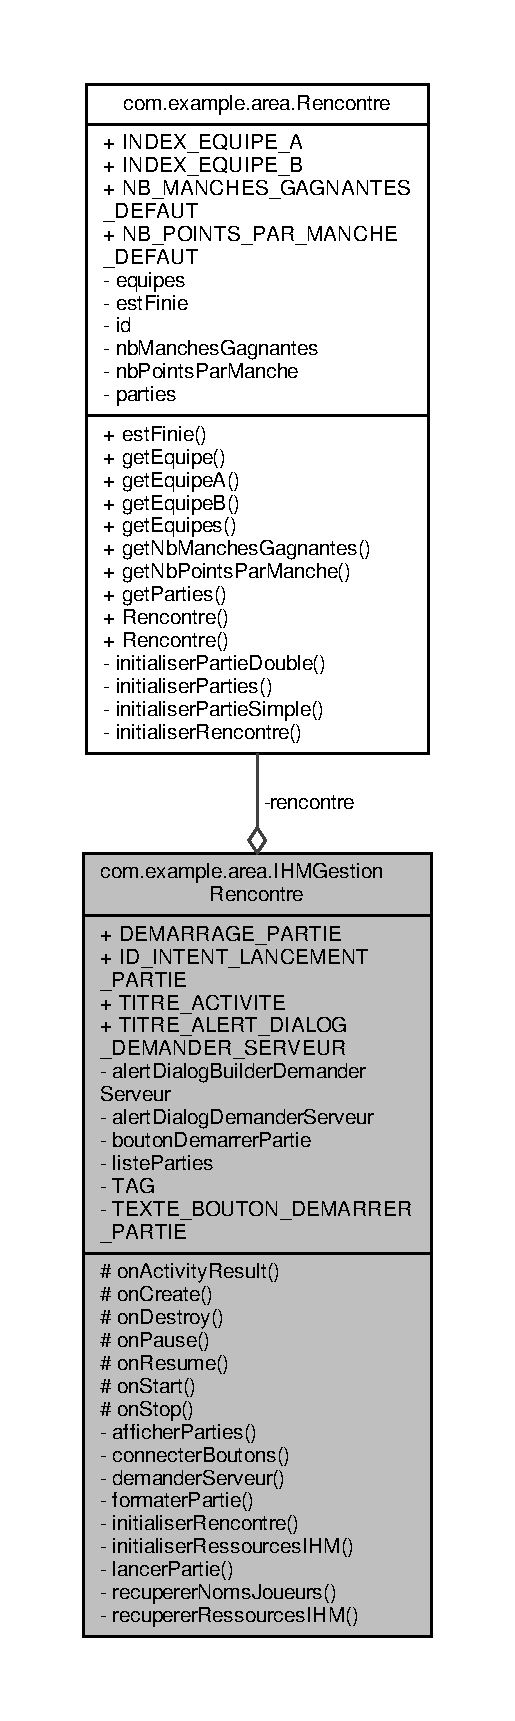
\includegraphics[height=550pt]{classcom_1_1example_1_1area_1_1_i_h_m_gestion_rencontre__coll__graph}
\end{center}
\end{figure}
\subsubsection*{Attributs publics statiques}
\begin{DoxyCompactItemize}
\item 
static final int \hyperlink{classcom_1_1example_1_1area_1_1_i_h_m_gestion_rencontre_a752975e509f051f66f3f06a744807f21}{D\+E\+M\+A\+R\+R\+A\+G\+E\+\_\+\+P\+A\+R\+T\+IE} = 0
\begin{DoxyCompactList}\small\item\em Code pour le lancement de l\textquotesingle{}activité \hyperlink{classcom_1_1example_1_1area_1_1_i_h_m_gestion_partie}{I\+H\+M\+Gestion\+Partie}. \end{DoxyCompactList}\item 
static final String \hyperlink{classcom_1_1example_1_1area_1_1_i_h_m_gestion_rencontre_a03e10549be0fc3fb5dc146afe8db5e89}{I\+D\+\_\+\+I\+N\+T\+E\+N\+T\+\_\+\+L\+A\+N\+C\+E\+M\+E\+N\+T\+\_\+\+P\+A\+R\+T\+IE} = \char`\"{}Partie\char`\"{}
\item 
static final String \hyperlink{classcom_1_1example_1_1area_1_1_i_h_m_gestion_rencontre_ae75a8de544fd03072c8dbaf6445d2589}{T\+I\+T\+R\+E\+\_\+\+A\+C\+T\+I\+V\+I\+TE} = \char`\"{}Liste des parties pour la \hyperlink{classcom_1_1example_1_1area_1_1_i_h_m_gestion_rencontre_aa3ecacbd8ab104d2a3c3f3e727ae6c5c}{rencontre} \+: \char`\"{}
\item 
static final String \hyperlink{classcom_1_1example_1_1area_1_1_i_h_m_gestion_rencontre_a31b8b293d8e0aa02050fddf9891349f2}{T\+I\+T\+R\+E\+\_\+\+A\+L\+E\+R\+T\+\_\+\+D\+I\+A\+L\+O\+G\+\_\+\+D\+E\+M\+A\+N\+D\+E\+R\+\_\+\+S\+E\+R\+V\+E\+UR} = \char`\"{}Veuillez sélectionner le premier joueur à servir \+:\char`\"{}
\end{DoxyCompactItemize}
\subsubsection*{Fonctions membres protégées}
\begin{DoxyCompactItemize}
\item 
void \hyperlink{classcom_1_1example_1_1area_1_1_i_h_m_gestion_rencontre_a2ab13355dbd1751f43ff54c534d0f021}{on\+Activity\+Result} (int request\+Code, int result\+Code, Intent data)
\begin{DoxyCompactList}\small\item\em Traite le retour de l\textquotesingle{}activité \hyperlink{classcom_1_1example_1_1area_1_1_i_h_m_gestion_partie}{I\+H\+M\+Gestion\+Partie}. \end{DoxyCompactList}\item 
void \hyperlink{classcom_1_1example_1_1area_1_1_i_h_m_gestion_rencontre_a233405b574407eda9ba407dd706fef91}{on\+Create} (Bundle saved\+Instance\+State)
\begin{DoxyCompactList}\small\item\em Méthode appelée à la création de l\textquotesingle{}activité \end{DoxyCompactList}\item 
void \hyperlink{classcom_1_1example_1_1area_1_1_i_h_m_gestion_rencontre_a0cee3ae4aa9559d72f43aaa62f4ebe75}{on\+Destroy} ()
\begin{DoxyCompactList}\small\item\em Méthode appelée à la destruction de l\textquotesingle{}application (après \hyperlink{classcom_1_1example_1_1area_1_1_i_h_m_gestion_rencontre_abfee40a2616713d70c0245ae72c6d794}{on\+Stop()} et détruite par le système Android) \end{DoxyCompactList}\item 
void \hyperlink{classcom_1_1example_1_1area_1_1_i_h_m_gestion_rencontre_a390adc8e9ec98d7147957ce8d9e1c071}{on\+Pause} ()
\begin{DoxyCompactList}\small\item\em Méthode appelée après qu\textquotesingle{}une boîte de dialogue s\textquotesingle{}est affichée (on reprend sur un \hyperlink{classcom_1_1example_1_1area_1_1_i_h_m_gestion_rencontre_ad8a4a274c61458fe25a48ccba0d846e7}{on\+Resume()}) ou avant \hyperlink{classcom_1_1example_1_1area_1_1_i_h_m_gestion_rencontre_abfee40a2616713d70c0245ae72c6d794}{on\+Stop()} (activité plus visible) \end{DoxyCompactList}\item 
void \hyperlink{classcom_1_1example_1_1area_1_1_i_h_m_gestion_rencontre_ad8a4a274c61458fe25a48ccba0d846e7}{on\+Resume} ()
\begin{DoxyCompactList}\small\item\em Méthode appelée après \hyperlink{classcom_1_1example_1_1area_1_1_i_h_m_gestion_rencontre_ae34fc2516b20ce7917e53eb9e55c7afc}{on\+Start()} ou après \hyperlink{classcom_1_1example_1_1area_1_1_i_h_m_gestion_rencontre_a390adc8e9ec98d7147957ce8d9e1c071}{on\+Pause()} \end{DoxyCompactList}\item 
void \hyperlink{classcom_1_1example_1_1area_1_1_i_h_m_gestion_rencontre_ae34fc2516b20ce7917e53eb9e55c7afc}{on\+Start} ()
\begin{DoxyCompactList}\small\item\em Méthode appelée au démarrage après le \hyperlink{classcom_1_1example_1_1area_1_1_i_h_m_gestion_rencontre_a233405b574407eda9ba407dd706fef91}{on\+Create()} ou un restart après un \hyperlink{classcom_1_1example_1_1area_1_1_i_h_m_gestion_rencontre_abfee40a2616713d70c0245ae72c6d794}{on\+Stop()} \end{DoxyCompactList}\item 
void \hyperlink{classcom_1_1example_1_1area_1_1_i_h_m_gestion_rencontre_abfee40a2616713d70c0245ae72c6d794}{on\+Stop} ()
\begin{DoxyCompactList}\small\item\em Méthode appelée lorsque l\textquotesingle{}activité n\textquotesingle{}est plus visible. \end{DoxyCompactList}\end{DoxyCompactItemize}
\subsubsection*{Fonctions membres privées}
\begin{DoxyCompactItemize}
\item 
void \hyperlink{classcom_1_1example_1_1area_1_1_i_h_m_gestion_rencontre_a5d86e4705a4bbea19f05781403df4742}{afficher\+Parties} ()
\begin{DoxyCompactList}\small\item\em Affiche une liste de toutes les parties d\textquotesingle{}une rencontre. \end{DoxyCompactList}\item 
void \hyperlink{classcom_1_1example_1_1area_1_1_i_h_m_gestion_rencontre_a3d4decb257b09dafa98f4a6accc8c15d}{connecter\+Boutons} ()
\begin{DoxyCompactList}\small\item\em Définit le comportement des boutons. \end{DoxyCompactList}\item 
void \hyperlink{classcom_1_1example_1_1area_1_1_i_h_m_gestion_rencontre_a34d405f3c30f6d040b2db3a6ee54a2f4}{demander\+Serveur} (\hyperlink{classcom_1_1example_1_1area_1_1_partie}{Partie} partie)
\begin{DoxyCompactList}\small\item\em Demande à l\textquotesingle{}utisateur qui est le premier à servir. \end{DoxyCompactList}\item 
String \hyperlink{classcom_1_1example_1_1area_1_1_i_h_m_gestion_rencontre_aadc556a63bb77b707f4677c34d61dae5}{formater\+Partie} (\hyperlink{classcom_1_1example_1_1area_1_1_partie}{Partie} partie)
\begin{DoxyCompactList}\small\item\em Formate une partie sous forme de String en respectant la structure suivante \+: \end{DoxyCompactList}\item 
void \hyperlink{classcom_1_1example_1_1area_1_1_i_h_m_gestion_rencontre_aedaadbb550aab497aac0501ced04a3eb}{initialiser\+Rencontre} ()
\begin{DoxyCompactList}\small\item\em Initialise un rencontre. \end{DoxyCompactList}\item 
void \hyperlink{classcom_1_1example_1_1area_1_1_i_h_m_gestion_rencontre_a18b1c1a04b6070a8d90aa135ad1212b7}{initialiser\+Ressources\+I\+HM} ()
\begin{DoxyCompactList}\small\item\em Initialise les ressources graphiques de l\textquotesingle{}activité \end{DoxyCompactList}\item 
void \hyperlink{classcom_1_1example_1_1area_1_1_i_h_m_gestion_rencontre_a284518fddedfaed4b257f852290e1e63}{lancer\+Partie} (\hyperlink{classcom_1_1example_1_1area_1_1_partie}{Partie} partie)
\begin{DoxyCompactList}\small\item\em Lance une partie. \end{DoxyCompactList}\item 
Char\+Sequence \mbox{[}$\,$\mbox{]} \hyperlink{classcom_1_1example_1_1area_1_1_i_h_m_gestion_rencontre_ae68b1e5d73d33d01e622a736a25da731}{recuperer\+Noms\+Joueurs} (Vector$<$ \hyperlink{classcom_1_1example_1_1area_1_1_joueur}{Joueur} $>$ joueursA, Vector$<$ \hyperlink{classcom_1_1example_1_1area_1_1_joueur}{Joueur} $>$ joueursB)
\begin{DoxyCompactList}\small\item\em Récupère les noms des joueurs et de leur club dans un tableau de Char\+Sequence. \end{DoxyCompactList}\item 
void \hyperlink{classcom_1_1example_1_1area_1_1_i_h_m_gestion_rencontre_ac3d024fe8637e7cc4469a88a7ab81b53}{recuperer\+Ressources\+I\+HM} ()
\begin{DoxyCompactList}\small\item\em Recupère les ressources graphiques de l\textquotesingle{}activité \end{DoxyCompactList}\end{DoxyCompactItemize}
\subsubsection*{Attributs privés}
\begin{DoxyCompactItemize}
\item 
Alert\+Dialog.\+Builder \hyperlink{classcom_1_1example_1_1area_1_1_i_h_m_gestion_rencontre_a47ed7018b2af1ac9197715b9008a34a5}{alert\+Dialog\+Builder\+Demander\+Serveur}
\item 
Alert\+Dialog \hyperlink{classcom_1_1example_1_1area_1_1_i_h_m_gestion_rencontre_a9e68d97c4b50758ce1d6a2d8a217d5fc}{alert\+Dialog\+Demander\+Serveur}
\item 
Button \hyperlink{classcom_1_1example_1_1area_1_1_i_h_m_gestion_rencontre_a29f52b3b1397d21728bbe60b826facd8}{bouton\+Demarrer\+Partie}
\item 
List\+View \hyperlink{classcom_1_1example_1_1area_1_1_i_h_m_gestion_rencontre_a127e07e7de6ff7e02fa84c52a3399aaa}{liste\+Parties}
\item 
\hyperlink{classcom_1_1example_1_1area_1_1_rencontre}{Rencontre} \hyperlink{classcom_1_1example_1_1area_1_1_i_h_m_gestion_rencontre_aa3ecacbd8ab104d2a3c3f3e727ae6c5c}{rencontre}
\end{DoxyCompactItemize}
\subsubsection*{Attributs privés statiques}
\begin{DoxyCompactItemize}
\item 
static final String \hyperlink{classcom_1_1example_1_1area_1_1_i_h_m_gestion_rencontre_a0ac4d9152d48619cd697c8c69166219f}{T\+AG} = \char`\"{}\+\_\+\+I\+H\+M\+Gestion\+Rencontre\char`\"{}
\begin{DoxyCompactList}\small\item\em T\+AG pour les logs. \end{DoxyCompactList}\item 
static final String \hyperlink{classcom_1_1example_1_1area_1_1_i_h_m_gestion_rencontre_abd01f503f5a75a27b12261b30d80c053}{T\+E\+X\+T\+E\+\_\+\+B\+O\+U\+T\+O\+N\+\_\+\+D\+E\+M\+A\+R\+R\+E\+R\+\_\+\+P\+A\+R\+T\+IE} = \char`\"{}Démarrer\char`\"{}
\end{DoxyCompactItemize}


\subsubsection{Description détaillée}
L\textquotesingle{}activité principale de l\textquotesingle{}application A\+R\+EA. 

Définition à la ligne \hyperlink{_i_h_m_gestion_rencontre_8java_source_l00035}{35} du fichier \hyperlink{_i_h_m_gestion_rencontre_8java_source}{I\+H\+M\+Gestion\+Rencontre.\+java}.



\subsubsection{Documentation des fonctions membres}
\mbox{\Hypertarget{classcom_1_1example_1_1area_1_1_i_h_m_gestion_rencontre_a5d86e4705a4bbea19f05781403df4742}\label{classcom_1_1example_1_1area_1_1_i_h_m_gestion_rencontre_a5d86e4705a4bbea19f05781403df4742}} 
\index{com\+::example\+::area\+::\+I\+H\+M\+Gestion\+Rencontre@{com\+::example\+::area\+::\+I\+H\+M\+Gestion\+Rencontre}!afficher\+Parties@{afficher\+Parties}}
\index{afficher\+Parties@{afficher\+Parties}!com\+::example\+::area\+::\+I\+H\+M\+Gestion\+Rencontre@{com\+::example\+::area\+::\+I\+H\+M\+Gestion\+Rencontre}}
\paragraph{\texorpdfstring{afficher\+Parties()}{afficherParties()}}
{\footnotesize\ttfamily void com.\+example.\+area.\+I\+H\+M\+Gestion\+Rencontre.\+afficher\+Parties (\begin{DoxyParamCaption}{ }\end{DoxyParamCaption})\hspace{0.3cm}{\ttfamily [private]}}



Affiche une liste de toutes les parties d\textquotesingle{}une rencontre. 



Définition à la ligne \hyperlink{_i_h_m_gestion_rencontre_8java_source_l00322}{322} du fichier \hyperlink{_i_h_m_gestion_rencontre_8java_source}{I\+H\+M\+Gestion\+Rencontre.\+java}.



Références \hyperlink{_i_h_m_gestion_rencontre_8java_source_l00343}{com.\+example.\+area.\+I\+H\+M\+Gestion\+Rencontre.\+formater\+Partie()}, et \hyperlink{_rencontre_8java_source_l00158}{com.\+example.\+area.\+Rencontre.\+get\+Parties()}.



Référencé par \hyperlink{_i_h_m_gestion_rencontre_8java_source_l00142}{com.\+example.\+area.\+I\+H\+M\+Gestion\+Rencontre.\+initialiser\+Ressources\+I\+H\+M()}.


\begin{DoxyCode}
00323     \{
00324         Vector<Partie> parties = \hyperlink{classcom_1_1example_1_1area_1_1_i_h_m_gestion_rencontre_aa3ecacbd8ab104d2a3c3f3e727ae6c5c}{rencontre}.\hyperlink{classcom_1_1example_1_1area_1_1_rencontre_a58b62bd2f8a63f532df2bc8607268a2d}{getParties}();
00325         ListIterator<Partie> it = parties.listIterator();
00326         ArrayList<String> arrayListParties = \textcolor{keyword}{new} ArrayList<String>();
00327         ArrayAdapter<String> adapter;
00328 
00329         \textcolor{keywordflow}{while}(it.hasNext())
00330         \{
00331             arrayListParties.add(\hyperlink{classcom_1_1example_1_1area_1_1_i_h_m_gestion_rencontre_aadc556a63bb77b707f4677c34d61dae5}{formaterPartie}(it.next()));
00332         \}
00333 
00334         adapter = \textcolor{keyword}{new} ArrayAdapter<String>(\textcolor{keyword}{this}, android.R.layout.simple\_list\_item\_single\_choice, 
      arrayListParties);
00335 
00336         \hyperlink{classcom_1_1example_1_1area_1_1_i_h_m_gestion_rencontre_a127e07e7de6ff7e02fa84c52a3399aaa}{listeParties}.setAdapter(adapter);
00337 
00338     \}
\end{DoxyCode}
\mbox{\Hypertarget{classcom_1_1example_1_1area_1_1_i_h_m_gestion_rencontre_a3d4decb257b09dafa98f4a6accc8c15d}\label{classcom_1_1example_1_1area_1_1_i_h_m_gestion_rencontre_a3d4decb257b09dafa98f4a6accc8c15d}} 
\index{com\+::example\+::area\+::\+I\+H\+M\+Gestion\+Rencontre@{com\+::example\+::area\+::\+I\+H\+M\+Gestion\+Rencontre}!connecter\+Boutons@{connecter\+Boutons}}
\index{connecter\+Boutons@{connecter\+Boutons}!com\+::example\+::area\+::\+I\+H\+M\+Gestion\+Rencontre@{com\+::example\+::area\+::\+I\+H\+M\+Gestion\+Rencontre}}
\paragraph{\texorpdfstring{connecter\+Boutons()}{connecterBoutons()}}
{\footnotesize\ttfamily void com.\+example.\+area.\+I\+H\+M\+Gestion\+Rencontre.\+connecter\+Boutons (\begin{DoxyParamCaption}{ }\end{DoxyParamCaption})\hspace{0.3cm}{\ttfamily [private]}}



Définit le comportement des boutons. 



Définition à la ligne \hyperlink{_i_h_m_gestion_rencontre_8java_source_l00158}{158} du fichier \hyperlink{_i_h_m_gestion_rencontre_8java_source}{I\+H\+M\+Gestion\+Rencontre.\+java}.



Références \hyperlink{_i_h_m_gestion_rencontre_8java_source_l00222}{com.\+example.\+area.\+I\+H\+M\+Gestion\+Rencontre.\+demander\+Serveur()}, et \hyperlink{_rencontre_8java_source_l00158}{com.\+example.\+area.\+Rencontre.\+get\+Parties()}.



Référencé par \hyperlink{_i_h_m_gestion_rencontre_8java_source_l00064}{com.\+example.\+area.\+I\+H\+M\+Gestion\+Rencontre.\+on\+Create()}.


\begin{DoxyCode}
00159     \{
00160         \hyperlink{classcom_1_1example_1_1area_1_1_i_h_m_gestion_rencontre_a29f52b3b1397d21728bbe60b826facd8}{boutonDemarrerPartie}.setOnClickListener(\textcolor{keyword}{new} View.OnClickListener()
00161         \{
00162             \textcolor{keyword}{public} \textcolor{keywordtype}{void} onClick(View v)
00163             \{
00164                 \hyperlink{classcom_1_1example_1_1area_1_1_i_h_m_gestion_rencontre_a34d405f3c30f6d040b2db3a6ee54a2f4}{demanderServeur}(\hyperlink{classcom_1_1example_1_1area_1_1_i_h_m_gestion_rencontre_aa3ecacbd8ab104d2a3c3f3e727ae6c5c}{rencontre}.\hyperlink{classcom_1_1example_1_1area_1_1_rencontre_a58b62bd2f8a63f532df2bc8607268a2d}{getParties}().elementAt(
      \hyperlink{classcom_1_1example_1_1area_1_1_i_h_m_gestion_rencontre_a127e07e7de6ff7e02fa84c52a3399aaa}{listeParties}.getCheckedItemPosition()));
00165             \}
00166         \});
00167 
00168         \hyperlink{classcom_1_1example_1_1area_1_1_i_h_m_gestion_rencontre_a127e07e7de6ff7e02fa84c52a3399aaa}{listeParties}.setOnItemClickListener(\textcolor{keyword}{new} AdapterView.OnItemClickListener()
00169         \{
00170             @Override
00171             \textcolor{keyword}{public} \textcolor{keywordtype}{void} onItemClick(AdapterView<?> parent, View view, \textcolor{keywordtype}{int} position, \textcolor{keywordtype}{long} \textcolor{keywordtype}{id})
00172             \{
00173                 Log.d(\hyperlink{classcom_1_1example_1_1area_1_1_i_h_m_gestion_rencontre_a0ac4d9152d48619cd697c8c69166219f}{TAG},\textcolor{stringliteral}{"onItemClick()"});
00174                 \hyperlink{classcom_1_1example_1_1area_1_1_i_h_m_gestion_rencontre_a127e07e7de6ff7e02fa84c52a3399aaa}{listeParties}.setItemChecked(position,\textcolor{keyword}{true});
00175 
00176             \}
00177         \});
00178     \}
\end{DoxyCode}
\mbox{\Hypertarget{classcom_1_1example_1_1area_1_1_i_h_m_gestion_rencontre_a34d405f3c30f6d040b2db3a6ee54a2f4}\label{classcom_1_1example_1_1area_1_1_i_h_m_gestion_rencontre_a34d405f3c30f6d040b2db3a6ee54a2f4}} 
\index{com\+::example\+::area\+::\+I\+H\+M\+Gestion\+Rencontre@{com\+::example\+::area\+::\+I\+H\+M\+Gestion\+Rencontre}!demander\+Serveur@{demander\+Serveur}}
\index{demander\+Serveur@{demander\+Serveur}!com\+::example\+::area\+::\+I\+H\+M\+Gestion\+Rencontre@{com\+::example\+::area\+::\+I\+H\+M\+Gestion\+Rencontre}}
\paragraph{\texorpdfstring{demander\+Serveur()}{demanderServeur()}}
{\footnotesize\ttfamily void com.\+example.\+area.\+I\+H\+M\+Gestion\+Rencontre.\+demander\+Serveur (\begin{DoxyParamCaption}\item[{\hyperlink{classcom_1_1example_1_1area_1_1_partie}{Partie}}]{partie }\end{DoxyParamCaption})\hspace{0.3cm}{\ttfamily [private]}}



Demande à l\textquotesingle{}utisateur qui est le premier à servir. 



Définition à la ligne \hyperlink{_i_h_m_gestion_rencontre_8java_source_l00222}{222} du fichier \hyperlink{_i_h_m_gestion_rencontre_8java_source}{I\+H\+M\+Gestion\+Rencontre.\+java}.



Références \hyperlink{_i_h_m_gestion_rencontre_8java_source_l00051}{com.\+example.\+area.\+I\+H\+M\+Gestion\+Rencontre.\+alert\+Dialog\+Builder\+Demander\+Serveur}, \hyperlink{_partie_8java_source_l00064}{com.\+example.\+area.\+Partie.\+get\+Joueurs\+A()}, \hyperlink{_partie_8java_source_l00072}{com.\+example.\+area.\+Partie.\+get\+Joueurs\+B()}, \hyperlink{_partie_8java_source_l00351}{com.\+example.\+area.\+Partie.\+get\+Nb\+Joueurs()}, \hyperlink{_i_h_m_gestion_rencontre_8java_source_l00311}{com.\+example.\+area.\+I\+H\+M\+Gestion\+Rencontre.\+lancer\+Partie()}, \hyperlink{_i_h_m_gestion_rencontre_8java_source_l00281}{com.\+example.\+area.\+I\+H\+M\+Gestion\+Rencontre.\+recuperer\+Noms\+Joueurs()}, \hyperlink{_partie_8java_source_l00359}{com.\+example.\+area.\+Partie.\+set\+Joueurs\+A()}, et \hyperlink{_partie_8java_source_l00367}{com.\+example.\+area.\+Partie.\+set\+Joueurs\+B()}.



Référencé par \hyperlink{_i_h_m_gestion_rencontre_8java_source_l00158}{com.\+example.\+area.\+I\+H\+M\+Gestion\+Rencontre.\+connecter\+Boutons()}.


\begin{DoxyCode}
00223     \{
00224         Vector<Joueur> joueursA = partie.getJoueursA();
00225         Vector<Joueur> joueursB = partie.getJoueursB();
00226         CharSequence[] nomJoueurs = \hyperlink{classcom_1_1example_1_1area_1_1_i_h_m_gestion_rencontre_ae68b1e5d73d33d01e622a736a25da731}{recupererNomsJoueurs}(joueursA, joueursB);
00227 
00228         \hyperlink{classcom_1_1example_1_1area_1_1_i_h_m_gestion_rencontre_a47ed7018b2af1ac9197715b9008a34a5}{alertDialogBuilderDemanderServeur}.setItems(nomJoueurs, \textcolor{keyword}{new} 
      DialogInterface.OnClickListener()
00229         \{
00230             \textcolor{keyword}{public} \textcolor{keywordtype}{void} onClick(DialogInterface dialog, \textcolor{keywordtype}{int} which)
00231             \{
00232                 \textcolor{comment}{// Partie simple ?}
00233                 \textcolor{keywordflow}{if}(partie.getNbJoueurs() == 2)
00234                 \{
00235                     \textcolor{keywordflow}{if}(which == 0)
00236                     \{
00237                         Log.d(\hyperlink{classcom_1_1example_1_1area_1_1_i_h_m_gestion_rencontre_a0ac4d9152d48619cd697c8c69166219f}{TAG},\textcolor{stringliteral}{"Serveur dans équipe A à la position : "} + which + \textcolor{stringliteral}{" ("} + joueursA.
      elementAt(which).getNom() + \textcolor{stringliteral}{")"});
00238                         joueursA.elementAt(which).setEstServeur(\textcolor{keyword}{true});
00239                         partie.setJoueursA(joueursA);
00240 
00241                     \}
00242                     \textcolor{keywordflow}{else}
00243                     \{
00244                         Log.d(\hyperlink{classcom_1_1example_1_1area_1_1_i_h_m_gestion_rencontre_a0ac4d9152d48619cd697c8c69166219f}{TAG},\textcolor{stringliteral}{"Serveur dans équipe B à la position : "} + (which-1) + \textcolor{stringliteral}{" ("} + joueursB
      .elementAt(which-1).getNom() + \textcolor{stringliteral}{")"});
00245                         joueursB.elementAt(which-1).setEstServeur(\textcolor{keyword}{true});
00246                         partie.setJoueursB(joueursB);
00247                     \}
00248                 \}
00249                 \textcolor{keywordflow}{else} \textcolor{keywordflow}{if}(partie.getNbJoueurs() == 4) \textcolor{comment}{// Partie double ?}
00250                 \{
00251                     \textcolor{keywordflow}{if}(which < 2)
00252                     \{
00253                         Log.d(\hyperlink{classcom_1_1example_1_1area_1_1_i_h_m_gestion_rencontre_a0ac4d9152d48619cd697c8c69166219f}{TAG},\textcolor{stringliteral}{"Serveur dans équipe A à la position : "} + which + \textcolor{stringliteral}{" ("} + joueursA.
      elementAt(which).getNom() + \textcolor{stringliteral}{")"});
00254                         joueursA.elementAt(which).setEstServeur(\textcolor{keyword}{true});
00255                         partie.setJoueursA(joueursA);
00256                     \}
00257                     \textcolor{keywordflow}{else}
00258                     \{
00259                         Log.d(\hyperlink{classcom_1_1example_1_1area_1_1_i_h_m_gestion_rencontre_a0ac4d9152d48619cd697c8c69166219f}{TAG},\textcolor{stringliteral}{"Serveur dans équipe B à la position : "} + (which-2) + \textcolor{stringliteral}{" ("} + joueursB
      .elementAt(which-2).getNom() + \textcolor{stringliteral}{")"});
00260                         joueursB.elementAt(which-2).setEstServeur(\textcolor{keyword}{true});
00261                         partie.setJoueursB(joueursB);
00262                     \}
00263                 \}
00264                 \textcolor{keywordflow}{else}
00265                 \{
00266                     Log.e(\hyperlink{classcom_1_1example_1_1area_1_1_i_h_m_gestion_rencontre_a0ac4d9152d48619cd697c8c69166219f}{TAG},\textcolor{stringliteral}{"Le nombre de joueurs dans cette partie est invalide !"});
00267                 \}
00268 
00269                 \hyperlink{classcom_1_1example_1_1area_1_1_i_h_m_gestion_rencontre_a284518fddedfaed4b257f852290e1e63}{lancerPartie}(partie);
00270             \}
00271         \});
00272 
00273         \hyperlink{classcom_1_1example_1_1area_1_1_i_h_m_gestion_rencontre_a9e68d97c4b50758ce1d6a2d8a217d5fc}{alertDialogDemanderServeur} = 
      \hyperlink{classcom_1_1example_1_1area_1_1_i_h_m_gestion_rencontre_a47ed7018b2af1ac9197715b9008a34a5}{alertDialogBuilderDemanderServeur}.create();
00274 
00275         \hyperlink{classcom_1_1example_1_1area_1_1_i_h_m_gestion_rencontre_a9e68d97c4b50758ce1d6a2d8a217d5fc}{alertDialogDemanderServeur}.show();
00276     \}
\end{DoxyCode}
\mbox{\Hypertarget{classcom_1_1example_1_1area_1_1_i_h_m_gestion_rencontre_aadc556a63bb77b707f4677c34d61dae5}\label{classcom_1_1example_1_1area_1_1_i_h_m_gestion_rencontre_aadc556a63bb77b707f4677c34d61dae5}} 
\index{com\+::example\+::area\+::\+I\+H\+M\+Gestion\+Rencontre@{com\+::example\+::area\+::\+I\+H\+M\+Gestion\+Rencontre}!formater\+Partie@{formater\+Partie}}
\index{formater\+Partie@{formater\+Partie}!com\+::example\+::area\+::\+I\+H\+M\+Gestion\+Rencontre@{com\+::example\+::area\+::\+I\+H\+M\+Gestion\+Rencontre}}
\paragraph{\texorpdfstring{formater\+Partie()}{formaterPartie()}}
{\footnotesize\ttfamily String com.\+example.\+area.\+I\+H\+M\+Gestion\+Rencontre.\+formater\+Partie (\begin{DoxyParamCaption}\item[{\hyperlink{classcom_1_1example_1_1area_1_1_partie}{Partie}}]{partie }\end{DoxyParamCaption})\hspace{0.3cm}{\ttfamily [private]}}



Formate une partie sous forme de String en respectant la structure suivante \+: 



Définition à la ligne \hyperlink{_i_h_m_gestion_rencontre_8java_source_l00343}{343} du fichier \hyperlink{_i_h_m_gestion_rencontre_8java_source}{I\+H\+M\+Gestion\+Rencontre.\+java}.



Références \hyperlink{_partie_8java_source_l00064}{com.\+example.\+area.\+Partie.\+get\+Joueurs\+A()}, \hyperlink{_partie_8java_source_l00072}{com.\+example.\+area.\+Partie.\+get\+Joueurs\+B()}, \hyperlink{_joueur_8java_source_l00039}{com.\+example.\+area.\+Joueur.\+get\+Nom()}, et \hyperlink{_joueur_8java_source_l00047}{com.\+example.\+area.\+Joueur.\+get\+Prenom()}.



Référencé par \hyperlink{_i_h_m_gestion_rencontre_8java_source_l00322}{com.\+example.\+area.\+I\+H\+M\+Gestion\+Rencontre.\+afficher\+Parties()}.


\begin{DoxyCode}
00344     \{
00345         String partieFormatee = \textcolor{keyword}{new} String();
00346         Vector<Joueur> joueursA = partie.getJoueursA();
00347         Vector<Joueur> joueursB = partie.getJoueursB();
00348         ListIterator<Joueur> it = joueursA.listIterator();
00349         Joueur joueur;
00350 
00351         \textcolor{keywordflow}{while} (it.hasNext())
00352         \{
00353             joueur = it.next();
00354             partieFormatee += joueur.getNom() + \textcolor{stringliteral}{" "} + joueur.getPrenom() + \textcolor{stringliteral}{" "};
00355         \}
00356 
00357         it = joueursB.listIterator();
00358         partieFormatee += \textcolor{stringliteral}{" VS  "};
00359 
00360         \textcolor{keywordflow}{while} (it.hasNext())
00361         \{
00362             joueur = it.next();
00363             partieFormatee += joueur.getNom() + \textcolor{stringliteral}{" "} + joueur.getPrenom() + \textcolor{stringliteral}{" "};
00364         \}
00365 
00366         \textcolor{keywordflow}{return} partieFormatee;
00367     \}
\end{DoxyCode}
\mbox{\Hypertarget{classcom_1_1example_1_1area_1_1_i_h_m_gestion_rencontre_aedaadbb550aab497aac0501ced04a3eb}\label{classcom_1_1example_1_1area_1_1_i_h_m_gestion_rencontre_aedaadbb550aab497aac0501ced04a3eb}} 
\index{com\+::example\+::area\+::\+I\+H\+M\+Gestion\+Rencontre@{com\+::example\+::area\+::\+I\+H\+M\+Gestion\+Rencontre}!initialiser\+Rencontre@{initialiser\+Rencontre}}
\index{initialiser\+Rencontre@{initialiser\+Rencontre}!com\+::example\+::area\+::\+I\+H\+M\+Gestion\+Rencontre@{com\+::example\+::area\+::\+I\+H\+M\+Gestion\+Rencontre}}
\paragraph{\texorpdfstring{initialiser\+Rencontre()}{initialiserRencontre()}}
{\footnotesize\ttfamily void com.\+example.\+area.\+I\+H\+M\+Gestion\+Rencontre.\+initialiser\+Rencontre (\begin{DoxyParamCaption}{ }\end{DoxyParamCaption})\hspace{0.3cm}{\ttfamily [private]}}



Initialise un rencontre. 



Définition à la ligne \hyperlink{_i_h_m_gestion_rencontre_8java_source_l00199}{199} du fichier \hyperlink{_i_h_m_gestion_rencontre_8java_source}{I\+H\+M\+Gestion\+Rencontre.\+java}.



Référencé par \hyperlink{_i_h_m_gestion_rencontre_8java_source_l00064}{com.\+example.\+area.\+I\+H\+M\+Gestion\+Rencontre.\+on\+Create()}.


\begin{DoxyCode}
00200     \{
00201         Vector<Joueur> joueursEquipe1 = \textcolor{keyword}{new} Vector<Joueur>();
00202         joueursEquipe1.add(\textcolor{keyword}{new} Joueur(\textcolor{stringliteral}{"BEAUMONT"},\textcolor{stringliteral}{"Jérôme"},843944));
00203         joueursEquipe1.add(\textcolor{keyword}{new} Joueur(\textcolor{stringliteral}{"SAULNIER"},\textcolor{stringliteral}{"Christian"},303504));
00204         joueursEquipe1.add(\textcolor{keyword}{new} Joueur(\textcolor{stringliteral}{"FILAFERRO"},\textcolor{stringliteral}{"Thomas"},645758));
00205         joueursEquipe1.add(\textcolor{keyword}{new} Joueur(\textcolor{stringliteral}{"COMTE"},\textcolor{stringliteral}{"Emmanuel"},842353));
00206 
00207         Vector<Joueur> joueursEquipe2 = \textcolor{keyword}{new} Vector<Joueur>();
00208         joueursEquipe2.add(\textcolor{keyword}{new} Joueur(\textcolor{stringliteral}{"FAGOO"},\textcolor{stringliteral}{"Damien"},844549));
00209         joueursEquipe2.add(\textcolor{keyword}{new} Joueur(\textcolor{stringliteral}{"BRESSON"},\textcolor{stringliteral}{"Thibault"},845423));
00210         joueursEquipe2.add(\textcolor{keyword}{new} Joueur(\textcolor{stringliteral}{"CROUZET"},\textcolor{stringliteral}{"Lionel"},845682));
00211         joueursEquipe2.add(\textcolor{keyword}{new} Joueur(\textcolor{stringliteral}{"FLORES"},\textcolor{stringliteral}{"Fabien"},847650));
00212 
00213         Equipe equipeA = \textcolor{keyword}{new} Equipe(\textcolor{stringliteral}{"PPC Sorgues"}, joueursEquipe1);
00214         Equipe equipeB = \textcolor{keyword}{new} Equipe(\textcolor{stringliteral}{"PPC Pernes"}, joueursEquipe2);
00215 
00216         this.\hyperlink{classcom_1_1example_1_1area_1_1_i_h_m_gestion_rencontre_aa3ecacbd8ab104d2a3c3f3e727ae6c5c}{rencontre} = \textcolor{keyword}{new} Rencontre(equipeA,equipeB);
00217     \}
\end{DoxyCode}
\mbox{\Hypertarget{classcom_1_1example_1_1area_1_1_i_h_m_gestion_rencontre_a18b1c1a04b6070a8d90aa135ad1212b7}\label{classcom_1_1example_1_1area_1_1_i_h_m_gestion_rencontre_a18b1c1a04b6070a8d90aa135ad1212b7}} 
\index{com\+::example\+::area\+::\+I\+H\+M\+Gestion\+Rencontre@{com\+::example\+::area\+::\+I\+H\+M\+Gestion\+Rencontre}!initialiser\+Ressources\+I\+HM@{initialiser\+Ressources\+I\+HM}}
\index{initialiser\+Ressources\+I\+HM@{initialiser\+Ressources\+I\+HM}!com\+::example\+::area\+::\+I\+H\+M\+Gestion\+Rencontre@{com\+::example\+::area\+::\+I\+H\+M\+Gestion\+Rencontre}}
\paragraph{\texorpdfstring{initialiser\+Ressources\+I\+H\+M()}{initialiserRessourcesIHM()}}
{\footnotesize\ttfamily void com.\+example.\+area.\+I\+H\+M\+Gestion\+Rencontre.\+initialiser\+Ressources\+I\+HM (\begin{DoxyParamCaption}{ }\end{DoxyParamCaption})\hspace{0.3cm}{\ttfamily [private]}}



Initialise les ressources graphiques de l\textquotesingle{}activité 



Définition à la ligne \hyperlink{_i_h_m_gestion_rencontre_8java_source_l00142}{142} du fichier \hyperlink{_i_h_m_gestion_rencontre_8java_source}{I\+H\+M\+Gestion\+Rencontre.\+java}.



Références \hyperlink{_i_h_m_gestion_rencontre_8java_source_l00322}{com.\+example.\+area.\+I\+H\+M\+Gestion\+Rencontre.\+afficher\+Parties()}, \hyperlink{_i_h_m_gestion_rencontre_8java_source_l00051}{com.\+example.\+area.\+I\+H\+M\+Gestion\+Rencontre.\+alert\+Dialog\+Builder\+Demander\+Serveur}, \hyperlink{_rencontre_8java_source_l00177}{com.\+example.\+area.\+Rencontre.\+get\+Equipe\+A()}, \hyperlink{_rencontre_8java_source_l00186}{com.\+example.\+area.\+Rencontre.\+get\+Equipe\+B()}, et \hyperlink{_equipe_8java_source_l00043}{com.\+example.\+area.\+Equipe.\+get\+Nom\+Club()}.



Référencé par \hyperlink{_i_h_m_gestion_rencontre_8java_source_l00064}{com.\+example.\+area.\+I\+H\+M\+Gestion\+Rencontre.\+on\+Create()}.


\begin{DoxyCode}
00143     \{
00144         \hyperlink{classcom_1_1example_1_1area_1_1_i_h_m_gestion_rencontre_a29f52b3b1397d21728bbe60b826facd8}{boutonDemarrerPartie}.setText(
      \hyperlink{classcom_1_1example_1_1area_1_1_i_h_m_gestion_rencontre_abd01f503f5a75a27b12261b30d80c053}{TEXTE\_BOUTON\_DEMARRER\_PARTIE});
00145 
00146         \hyperlink{classcom_1_1example_1_1area_1_1_i_h_m_gestion_rencontre_a47ed7018b2af1ac9197715b9008a34a5}{alertDialogBuilderDemanderServeur}.setTitle(
      \hyperlink{classcom_1_1example_1_1area_1_1_i_h_m_gestion_rencontre_a31b8b293d8e0aa02050fddf9891349f2}{TITRE\_ALERT\_DIALOG\_DEMANDER\_SERVEUR});
00147 
00148         \hyperlink{classcom_1_1example_1_1area_1_1_i_h_m_gestion_rencontre_a9e68d97c4b50758ce1d6a2d8a217d5fc}{alertDialogDemanderServeur} = 
      \hyperlink{classcom_1_1example_1_1area_1_1_i_h_m_gestion_rencontre_a47ed7018b2af1ac9197715b9008a34a5}{alertDialogBuilderDemanderServeur}.create();
00149 
00150         \hyperlink{classcom_1_1example_1_1area_1_1_i_h_m_gestion_rencontre_a5d86e4705a4bbea19f05781403df4742}{afficherParties}();
00151 
00152         getSupportActionBar().setTitle( \hyperlink{classcom_1_1example_1_1area_1_1_i_h_m_gestion_rencontre_ae75a8de544fd03072c8dbaf6445d2589}{TITRE\_ACTIVITE} + \hyperlink{classcom_1_1example_1_1area_1_1_i_h_m_gestion_rencontre_aa3ecacbd8ab104d2a3c3f3e727ae6c5c}{rencontre}.
      \hyperlink{classcom_1_1example_1_1area_1_1_rencontre_a207498fd691285b28b0a720da0a660f8}{getEquipeA}().\hyperlink{classcom_1_1example_1_1area_1_1_equipe_a735e5e0aaac9ac2c17f3eca3d47862dc}{getNomClub}() + \textcolor{stringliteral}{" VS "} + \hyperlink{classcom_1_1example_1_1area_1_1_i_h_m_gestion_rencontre_aa3ecacbd8ab104d2a3c3f3e727ae6c5c}{rencontre}.
      \hyperlink{classcom_1_1example_1_1area_1_1_rencontre_a83deec026e26407049c5671672291170}{getEquipeB}().\hyperlink{classcom_1_1example_1_1area_1_1_equipe_a735e5e0aaac9ac2c17f3eca3d47862dc}{getNomClub}());
00153     \}
\end{DoxyCode}
\mbox{\Hypertarget{classcom_1_1example_1_1area_1_1_i_h_m_gestion_rencontre_a284518fddedfaed4b257f852290e1e63}\label{classcom_1_1example_1_1area_1_1_i_h_m_gestion_rencontre_a284518fddedfaed4b257f852290e1e63}} 
\index{com\+::example\+::area\+::\+I\+H\+M\+Gestion\+Rencontre@{com\+::example\+::area\+::\+I\+H\+M\+Gestion\+Rencontre}!lancer\+Partie@{lancer\+Partie}}
\index{lancer\+Partie@{lancer\+Partie}!com\+::example\+::area\+::\+I\+H\+M\+Gestion\+Rencontre@{com\+::example\+::area\+::\+I\+H\+M\+Gestion\+Rencontre}}
\paragraph{\texorpdfstring{lancer\+Partie()}{lancerPartie()}}
{\footnotesize\ttfamily void com.\+example.\+area.\+I\+H\+M\+Gestion\+Rencontre.\+lancer\+Partie (\begin{DoxyParamCaption}\item[{\hyperlink{classcom_1_1example_1_1area_1_1_partie}{Partie}}]{partie }\end{DoxyParamCaption})\hspace{0.3cm}{\ttfamily [private]}}



Lance une partie. 


\begin{DoxyParams}{Paramètres}
{\em partie} & La partie à lancer \\
\hline
\end{DoxyParams}


Définition à la ligne \hyperlink{_i_h_m_gestion_rencontre_8java_source_l00311}{311} du fichier \hyperlink{_i_h_m_gestion_rencontre_8java_source}{I\+H\+M\+Gestion\+Rencontre.\+java}.



Référencé par \hyperlink{_i_h_m_gestion_rencontre_8java_source_l00222}{com.\+example.\+area.\+I\+H\+M\+Gestion\+Rencontre.\+demander\+Serveur()}.


\begin{DoxyCode}
00312     \{
00313         \textcolor{keyword}{final} Intent intent = \textcolor{keyword}{new} Intent(IHMGestionRencontre.this, IHMGestionPartie.class);
00314         intent.putExtra(\hyperlink{classcom_1_1example_1_1area_1_1_i_h_m_gestion_rencontre_a03e10549be0fc3fb5dc146afe8db5e89}{ID\_INTENT\_LANCEMENT\_PARTIE}, partie);
00315         Log.d(\hyperlink{classcom_1_1example_1_1area_1_1_i_h_m_gestion_rencontre_a0ac4d9152d48619cd697c8c69166219f}{TAG},\textcolor{stringliteral}{"Lancement de l'activité IHMGestionPartie"});
00316         startActivityForResult(intent, \hyperlink{classcom_1_1example_1_1area_1_1_i_h_m_gestion_rencontre_a752975e509f051f66f3f06a744807f21}{DEMARRAGE\_PARTIE});
00317     \}
\end{DoxyCode}
\mbox{\Hypertarget{classcom_1_1example_1_1area_1_1_i_h_m_gestion_rencontre_a2ab13355dbd1751f43ff54c534d0f021}\label{classcom_1_1example_1_1area_1_1_i_h_m_gestion_rencontre_a2ab13355dbd1751f43ff54c534d0f021}} 
\index{com\+::example\+::area\+::\+I\+H\+M\+Gestion\+Rencontre@{com\+::example\+::area\+::\+I\+H\+M\+Gestion\+Rencontre}!on\+Activity\+Result@{on\+Activity\+Result}}
\index{on\+Activity\+Result@{on\+Activity\+Result}!com\+::example\+::area\+::\+I\+H\+M\+Gestion\+Rencontre@{com\+::example\+::area\+::\+I\+H\+M\+Gestion\+Rencontre}}
\paragraph{\texorpdfstring{on\+Activity\+Result()}{onActivityResult()}}
{\footnotesize\ttfamily void com.\+example.\+area.\+I\+H\+M\+Gestion\+Rencontre.\+on\+Activity\+Result (\begin{DoxyParamCaption}\item[{int}]{request\+Code,  }\item[{int}]{result\+Code,  }\item[{Intent}]{data }\end{DoxyParamCaption})\hspace{0.3cm}{\ttfamily [protected]}}



Traite le retour de l\textquotesingle{}activité \hyperlink{classcom_1_1example_1_1area_1_1_i_h_m_gestion_partie}{I\+H\+M\+Gestion\+Partie}. 



Définition à la ligne \hyperlink{_i_h_m_gestion_rencontre_8java_source_l00184}{184} du fichier \hyperlink{_i_h_m_gestion_rencontre_8java_source}{I\+H\+M\+Gestion\+Rencontre.\+java}.


\begin{DoxyCode}
00185     \{
00186         super.onActivityResult(requestCode, resultCode, data);
00187         Log.d(\hyperlink{classcom_1_1example_1_1area_1_1_i_h_m_gestion_rencontre_a0ac4d9152d48619cd697c8c69166219f}{TAG}, \textcolor{stringliteral}{"onActivityResult() resultCode : "} + resultCode);
00188 
00189         \textcolor{comment}{// Exemple}
00190         \textcolor{keywordflow}{if}(requestCode == \hyperlink{classcom_1_1example_1_1area_1_1_i_h_m_gestion_rencontre_a752975e509f051f66f3f06a744807f21}{DEMARRAGE\_PARTIE} && resultCode == RESULT\_OK)
00191         \{
00192             Log.d(\hyperlink{classcom_1_1example_1_1area_1_1_i_h_m_gestion_rencontre_a0ac4d9152d48619cd697c8c69166219f}{TAG}, \textcolor{stringliteral}{"onActivityResult() IHMGestionPartie s'est terminée avec succès !"});
00193         \}
00194     \}
\end{DoxyCode}
\mbox{\Hypertarget{classcom_1_1example_1_1area_1_1_i_h_m_gestion_rencontre_a233405b574407eda9ba407dd706fef91}\label{classcom_1_1example_1_1area_1_1_i_h_m_gestion_rencontre_a233405b574407eda9ba407dd706fef91}} 
\index{com\+::example\+::area\+::\+I\+H\+M\+Gestion\+Rencontre@{com\+::example\+::area\+::\+I\+H\+M\+Gestion\+Rencontre}!on\+Create@{on\+Create}}
\index{on\+Create@{on\+Create}!com\+::example\+::area\+::\+I\+H\+M\+Gestion\+Rencontre@{com\+::example\+::area\+::\+I\+H\+M\+Gestion\+Rencontre}}
\paragraph{\texorpdfstring{on\+Create()}{onCreate()}}
{\footnotesize\ttfamily void com.\+example.\+area.\+I\+H\+M\+Gestion\+Rencontre.\+on\+Create (\begin{DoxyParamCaption}\item[{Bundle}]{saved\+Instance\+State }\end{DoxyParamCaption})\hspace{0.3cm}{\ttfamily [protected]}}



Méthode appelée à la création de l\textquotesingle{}activité 



Définition à la ligne \hyperlink{_i_h_m_gestion_rencontre_8java_source_l00064}{64} du fichier \hyperlink{_i_h_m_gestion_rencontre_8java_source}{I\+H\+M\+Gestion\+Rencontre.\+java}.



Références \hyperlink{_i_h_m_gestion_rencontre_8java_source_l00158}{com.\+example.\+area.\+I\+H\+M\+Gestion\+Rencontre.\+connecter\+Boutons()}, \hyperlink{_i_h_m_gestion_rencontre_8java_source_l00199}{com.\+example.\+area.\+I\+H\+M\+Gestion\+Rencontre.\+initialiser\+Rencontre()}, \hyperlink{_i_h_m_gestion_rencontre_8java_source_l00142}{com.\+example.\+area.\+I\+H\+M\+Gestion\+Rencontre.\+initialiser\+Ressources\+I\+H\+M()}, et \hyperlink{_i_h_m_gestion_rencontre_8java_source_l00132}{com.\+example.\+area.\+I\+H\+M\+Gestion\+Rencontre.\+recuperer\+Ressources\+I\+H\+M()}.


\begin{DoxyCode}
00065     \{
00066         super.onCreate(savedInstanceState);
00067         setContentView(R.layout.ihm\_gestion\_rencontre);
00068         Log.d(\hyperlink{classcom_1_1example_1_1area_1_1_i_h_m_gestion_rencontre_a0ac4d9152d48619cd697c8c69166219f}{TAG}, \textcolor{stringliteral}{"onCreate()"});
00069 
00070         \hyperlink{classcom_1_1example_1_1area_1_1_i_h_m_gestion_rencontre_aedaadbb550aab497aac0501ced04a3eb}{initialiserRencontre}();
00071 
00072         \hyperlink{classcom_1_1example_1_1area_1_1_i_h_m_gestion_rencontre_ac3d024fe8637e7cc4469a88a7ab81b53}{recupererRessourcesIHM}();
00073 
00074         \hyperlink{classcom_1_1example_1_1area_1_1_i_h_m_gestion_rencontre_a18b1c1a04b6070a8d90aa135ad1212b7}{initialiserRessourcesIHM}();
00075 
00076         \hyperlink{classcom_1_1example_1_1area_1_1_i_h_m_gestion_rencontre_a3d4decb257b09dafa98f4a6accc8c15d}{connecterBoutons}();
00077     \}
\end{DoxyCode}
\mbox{\Hypertarget{classcom_1_1example_1_1area_1_1_i_h_m_gestion_rencontre_a0cee3ae4aa9559d72f43aaa62f4ebe75}\label{classcom_1_1example_1_1area_1_1_i_h_m_gestion_rencontre_a0cee3ae4aa9559d72f43aaa62f4ebe75}} 
\index{com\+::example\+::area\+::\+I\+H\+M\+Gestion\+Rencontre@{com\+::example\+::area\+::\+I\+H\+M\+Gestion\+Rencontre}!on\+Destroy@{on\+Destroy}}
\index{on\+Destroy@{on\+Destroy}!com\+::example\+::area\+::\+I\+H\+M\+Gestion\+Rencontre@{com\+::example\+::area\+::\+I\+H\+M\+Gestion\+Rencontre}}
\paragraph{\texorpdfstring{on\+Destroy()}{onDestroy()}}
{\footnotesize\ttfamily void com.\+example.\+area.\+I\+H\+M\+Gestion\+Rencontre.\+on\+Destroy (\begin{DoxyParamCaption}{ }\end{DoxyParamCaption})\hspace{0.3cm}{\ttfamily [protected]}}



Méthode appelée à la destruction de l\textquotesingle{}application (après \hyperlink{classcom_1_1example_1_1area_1_1_i_h_m_gestion_rencontre_abfee40a2616713d70c0245ae72c6d794}{on\+Stop()} et détruite par le système Android) 



Définition à la ligne \hyperlink{_i_h_m_gestion_rencontre_8java_source_l00123}{123} du fichier \hyperlink{_i_h_m_gestion_rencontre_8java_source}{I\+H\+M\+Gestion\+Rencontre.\+java}.


\begin{DoxyCode}
00124     \{
00125         super.onDestroy();
00126         Log.d(\hyperlink{classcom_1_1example_1_1area_1_1_i_h_m_gestion_rencontre_a0ac4d9152d48619cd697c8c69166219f}{TAG}, \textcolor{stringliteral}{"onDestroy()"});
00127     \}
\end{DoxyCode}
\mbox{\Hypertarget{classcom_1_1example_1_1area_1_1_i_h_m_gestion_rencontre_a390adc8e9ec98d7147957ce8d9e1c071}\label{classcom_1_1example_1_1area_1_1_i_h_m_gestion_rencontre_a390adc8e9ec98d7147957ce8d9e1c071}} 
\index{com\+::example\+::area\+::\+I\+H\+M\+Gestion\+Rencontre@{com\+::example\+::area\+::\+I\+H\+M\+Gestion\+Rencontre}!on\+Pause@{on\+Pause}}
\index{on\+Pause@{on\+Pause}!com\+::example\+::area\+::\+I\+H\+M\+Gestion\+Rencontre@{com\+::example\+::area\+::\+I\+H\+M\+Gestion\+Rencontre}}
\paragraph{\texorpdfstring{on\+Pause()}{onPause()}}
{\footnotesize\ttfamily void com.\+example.\+area.\+I\+H\+M\+Gestion\+Rencontre.\+on\+Pause (\begin{DoxyParamCaption}{ }\end{DoxyParamCaption})\hspace{0.3cm}{\ttfamily [protected]}}



Méthode appelée après qu\textquotesingle{}une boîte de dialogue s\textquotesingle{}est affichée (on reprend sur un \hyperlink{classcom_1_1example_1_1area_1_1_i_h_m_gestion_rencontre_ad8a4a274c61458fe25a48ccba0d846e7}{on\+Resume()}) ou avant \hyperlink{classcom_1_1example_1_1area_1_1_i_h_m_gestion_rencontre_abfee40a2616713d70c0245ae72c6d794}{on\+Stop()} (activité plus visible) 



Définition à la ligne \hyperlink{_i_h_m_gestion_rencontre_8java_source_l00103}{103} du fichier \hyperlink{_i_h_m_gestion_rencontre_8java_source}{I\+H\+M\+Gestion\+Rencontre.\+java}.


\begin{DoxyCode}
00104     \{
00105         super.onPause();
00106         Log.d(\hyperlink{classcom_1_1example_1_1area_1_1_i_h_m_gestion_rencontre_a0ac4d9152d48619cd697c8c69166219f}{TAG}, \textcolor{stringliteral}{"onPause()"});
00107     \}
\end{DoxyCode}
\mbox{\Hypertarget{classcom_1_1example_1_1area_1_1_i_h_m_gestion_rencontre_ad8a4a274c61458fe25a48ccba0d846e7}\label{classcom_1_1example_1_1area_1_1_i_h_m_gestion_rencontre_ad8a4a274c61458fe25a48ccba0d846e7}} 
\index{com\+::example\+::area\+::\+I\+H\+M\+Gestion\+Rencontre@{com\+::example\+::area\+::\+I\+H\+M\+Gestion\+Rencontre}!on\+Resume@{on\+Resume}}
\index{on\+Resume@{on\+Resume}!com\+::example\+::area\+::\+I\+H\+M\+Gestion\+Rencontre@{com\+::example\+::area\+::\+I\+H\+M\+Gestion\+Rencontre}}
\paragraph{\texorpdfstring{on\+Resume()}{onResume()}}
{\footnotesize\ttfamily void com.\+example.\+area.\+I\+H\+M\+Gestion\+Rencontre.\+on\+Resume (\begin{DoxyParamCaption}{ }\end{DoxyParamCaption})\hspace{0.3cm}{\ttfamily [protected]}}



Méthode appelée après \hyperlink{classcom_1_1example_1_1area_1_1_i_h_m_gestion_rencontre_ae34fc2516b20ce7917e53eb9e55c7afc}{on\+Start()} ou après \hyperlink{classcom_1_1example_1_1area_1_1_i_h_m_gestion_rencontre_a390adc8e9ec98d7147957ce8d9e1c071}{on\+Pause()} 



Définition à la ligne \hyperlink{_i_h_m_gestion_rencontre_8java_source_l00093}{93} du fichier \hyperlink{_i_h_m_gestion_rencontre_8java_source}{I\+H\+M\+Gestion\+Rencontre.\+java}.


\begin{DoxyCode}
00094     \{
00095         super.onResume();
00096         Log.d(\hyperlink{classcom_1_1example_1_1area_1_1_i_h_m_gestion_rencontre_a0ac4d9152d48619cd697c8c69166219f}{TAG}, \textcolor{stringliteral}{"onResume()"});
00097     \}
\end{DoxyCode}
\mbox{\Hypertarget{classcom_1_1example_1_1area_1_1_i_h_m_gestion_rencontre_ae34fc2516b20ce7917e53eb9e55c7afc}\label{classcom_1_1example_1_1area_1_1_i_h_m_gestion_rencontre_ae34fc2516b20ce7917e53eb9e55c7afc}} 
\index{com\+::example\+::area\+::\+I\+H\+M\+Gestion\+Rencontre@{com\+::example\+::area\+::\+I\+H\+M\+Gestion\+Rencontre}!on\+Start@{on\+Start}}
\index{on\+Start@{on\+Start}!com\+::example\+::area\+::\+I\+H\+M\+Gestion\+Rencontre@{com\+::example\+::area\+::\+I\+H\+M\+Gestion\+Rencontre}}
\paragraph{\texorpdfstring{on\+Start()}{onStart()}}
{\footnotesize\ttfamily void com.\+example.\+area.\+I\+H\+M\+Gestion\+Rencontre.\+on\+Start (\begin{DoxyParamCaption}{ }\end{DoxyParamCaption})\hspace{0.3cm}{\ttfamily [protected]}}



Méthode appelée au démarrage après le \hyperlink{classcom_1_1example_1_1area_1_1_i_h_m_gestion_rencontre_a233405b574407eda9ba407dd706fef91}{on\+Create()} ou un restart après un \hyperlink{classcom_1_1example_1_1area_1_1_i_h_m_gestion_rencontre_abfee40a2616713d70c0245ae72c6d794}{on\+Stop()} 



Définition à la ligne \hyperlink{_i_h_m_gestion_rencontre_8java_source_l00083}{83} du fichier \hyperlink{_i_h_m_gestion_rencontre_8java_source}{I\+H\+M\+Gestion\+Rencontre.\+java}.


\begin{DoxyCode}
00084     \{
00085         super.onStart();
00086         Log.d(\hyperlink{classcom_1_1example_1_1area_1_1_i_h_m_gestion_rencontre_a0ac4d9152d48619cd697c8c69166219f}{TAG}, \textcolor{stringliteral}{"onStart()"});
00087     \}
\end{DoxyCode}
\mbox{\Hypertarget{classcom_1_1example_1_1area_1_1_i_h_m_gestion_rencontre_abfee40a2616713d70c0245ae72c6d794}\label{classcom_1_1example_1_1area_1_1_i_h_m_gestion_rencontre_abfee40a2616713d70c0245ae72c6d794}} 
\index{com\+::example\+::area\+::\+I\+H\+M\+Gestion\+Rencontre@{com\+::example\+::area\+::\+I\+H\+M\+Gestion\+Rencontre}!on\+Stop@{on\+Stop}}
\index{on\+Stop@{on\+Stop}!com\+::example\+::area\+::\+I\+H\+M\+Gestion\+Rencontre@{com\+::example\+::area\+::\+I\+H\+M\+Gestion\+Rencontre}}
\paragraph{\texorpdfstring{on\+Stop()}{onStop()}}
{\footnotesize\ttfamily void com.\+example.\+area.\+I\+H\+M\+Gestion\+Rencontre.\+on\+Stop (\begin{DoxyParamCaption}{ }\end{DoxyParamCaption})\hspace{0.3cm}{\ttfamily [protected]}}



Méthode appelée lorsque l\textquotesingle{}activité n\textquotesingle{}est plus visible. 



Définition à la ligne \hyperlink{_i_h_m_gestion_rencontre_8java_source_l00113}{113} du fichier \hyperlink{_i_h_m_gestion_rencontre_8java_source}{I\+H\+M\+Gestion\+Rencontre.\+java}.


\begin{DoxyCode}
00114     \{
00115         super.onStop();
00116         Log.d(\hyperlink{classcom_1_1example_1_1area_1_1_i_h_m_gestion_rencontre_a0ac4d9152d48619cd697c8c69166219f}{TAG}, \textcolor{stringliteral}{"onStop()"});
00117     \}
\end{DoxyCode}
\mbox{\Hypertarget{classcom_1_1example_1_1area_1_1_i_h_m_gestion_rencontre_ae68b1e5d73d33d01e622a736a25da731}\label{classcom_1_1example_1_1area_1_1_i_h_m_gestion_rencontre_ae68b1e5d73d33d01e622a736a25da731}} 
\index{com\+::example\+::area\+::\+I\+H\+M\+Gestion\+Rencontre@{com\+::example\+::area\+::\+I\+H\+M\+Gestion\+Rencontre}!recuperer\+Noms\+Joueurs@{recuperer\+Noms\+Joueurs}}
\index{recuperer\+Noms\+Joueurs@{recuperer\+Noms\+Joueurs}!com\+::example\+::area\+::\+I\+H\+M\+Gestion\+Rencontre@{com\+::example\+::area\+::\+I\+H\+M\+Gestion\+Rencontre}}
\paragraph{\texorpdfstring{recuperer\+Noms\+Joueurs()}{recupererNomsJoueurs()}}
{\footnotesize\ttfamily Char\+Sequence \mbox{[}$\,$\mbox{]} com.\+example.\+area.\+I\+H\+M\+Gestion\+Rencontre.\+recuperer\+Noms\+Joueurs (\begin{DoxyParamCaption}\item[{Vector$<$ \hyperlink{classcom_1_1example_1_1area_1_1_joueur}{Joueur} $>$}]{joueursA,  }\item[{Vector$<$ \hyperlink{classcom_1_1example_1_1area_1_1_joueur}{Joueur} $>$}]{joueursB }\end{DoxyParamCaption})\hspace{0.3cm}{\ttfamily [private]}}



Récupère les noms des joueurs et de leur club dans un tableau de Char\+Sequence. 



Définition à la ligne \hyperlink{_i_h_m_gestion_rencontre_8java_source_l00281}{281} du fichier \hyperlink{_i_h_m_gestion_rencontre_8java_source}{I\+H\+M\+Gestion\+Rencontre.\+java}.



Références \hyperlink{_rencontre_8java_source_l00177}{com.\+example.\+area.\+Rencontre.\+get\+Equipe\+A()}, \hyperlink{_rencontre_8java_source_l00186}{com.\+example.\+area.\+Rencontre.\+get\+Equipe\+B()}, \hyperlink{_joueur_8java_source_l00039}{com.\+example.\+area.\+Joueur.\+get\+Nom()}, \hyperlink{_equipe_8java_source_l00043}{com.\+example.\+area.\+Equipe.\+get\+Nom\+Club()}, et \hyperlink{_joueur_8java_source_l00047}{com.\+example.\+area.\+Joueur.\+get\+Prenom()}.



Référencé par \hyperlink{_i_h_m_gestion_rencontre_8java_source_l00222}{com.\+example.\+area.\+I\+H\+M\+Gestion\+Rencontre.\+demander\+Serveur()}.


\begin{DoxyCode}
00282     \{
00283         \textcolor{keywordtype}{int} nbJoueurs = joueursA.size() + joueursB.size();
00284         CharSequence nomJoueurs[] = \textcolor{keyword}{new} CharSequence[nbJoueurs];
00285         ListIterator<Joueur> it = joueursA.listIterator();
00286         \textcolor{keywordtype}{int} i = 0;
00287         Joueur joueur;
00288 
00289         \textcolor{keywordflow}{while} (it.hasNext())
00290         \{
00291             joueur = it.next();
00292             nomJoueurs[i] = \textcolor{stringliteral}{"[ "} + \hyperlink{classcom_1_1example_1_1area_1_1_i_h_m_gestion_rencontre_aa3ecacbd8ab104d2a3c3f3e727ae6c5c}{rencontre}.\hyperlink{classcom_1_1example_1_1area_1_1_rencontre_a207498fd691285b28b0a720da0a660f8}{getEquipeA}().
      \hyperlink{classcom_1_1example_1_1area_1_1_equipe_a735e5e0aaac9ac2c17f3eca3d47862dc}{getNomClub}() + \textcolor{stringliteral}{"] "} + joueur.getNom()+ \textcolor{stringliteral}{" "} + joueur.getPrenom();
00293             i++;
00294         \}
00295 
00296         it = joueursB.listIterator();
00297 
00298         \textcolor{keywordflow}{while} (it.hasNext())
00299         \{
00300             joueur = it.next();
00301             nomJoueurs[i] = \textcolor{stringliteral}{"[ "} + \hyperlink{classcom_1_1example_1_1area_1_1_i_h_m_gestion_rencontre_aa3ecacbd8ab104d2a3c3f3e727ae6c5c}{rencontre}.\hyperlink{classcom_1_1example_1_1area_1_1_rencontre_a83deec026e26407049c5671672291170}{getEquipeB}().
      \hyperlink{classcom_1_1example_1_1area_1_1_equipe_a735e5e0aaac9ac2c17f3eca3d47862dc}{getNomClub}() + \textcolor{stringliteral}{"] "} + joueur.getNom()+ \textcolor{stringliteral}{" "} + joueur.getPrenom();
00302             i++;
00303         \}
00304         \textcolor{keywordflow}{return} nomJoueurs;
00305     \}
\end{DoxyCode}
\mbox{\Hypertarget{classcom_1_1example_1_1area_1_1_i_h_m_gestion_rencontre_ac3d024fe8637e7cc4469a88a7ab81b53}\label{classcom_1_1example_1_1area_1_1_i_h_m_gestion_rencontre_ac3d024fe8637e7cc4469a88a7ab81b53}} 
\index{com\+::example\+::area\+::\+I\+H\+M\+Gestion\+Rencontre@{com\+::example\+::area\+::\+I\+H\+M\+Gestion\+Rencontre}!recuperer\+Ressources\+I\+HM@{recuperer\+Ressources\+I\+HM}}
\index{recuperer\+Ressources\+I\+HM@{recuperer\+Ressources\+I\+HM}!com\+::example\+::area\+::\+I\+H\+M\+Gestion\+Rencontre@{com\+::example\+::area\+::\+I\+H\+M\+Gestion\+Rencontre}}
\paragraph{\texorpdfstring{recuperer\+Ressources\+I\+H\+M()}{recupererRessourcesIHM()}}
{\footnotesize\ttfamily void com.\+example.\+area.\+I\+H\+M\+Gestion\+Rencontre.\+recuperer\+Ressources\+I\+HM (\begin{DoxyParamCaption}{ }\end{DoxyParamCaption})\hspace{0.3cm}{\ttfamily [private]}}



Recupère les ressources graphiques de l\textquotesingle{}activité 



Définition à la ligne \hyperlink{_i_h_m_gestion_rencontre_8java_source_l00132}{132} du fichier \hyperlink{_i_h_m_gestion_rencontre_8java_source}{I\+H\+M\+Gestion\+Rencontre.\+java}.



Références \hyperlink{_i_h_m_gestion_rencontre_8java_source_l00051}{com.\+example.\+area.\+I\+H\+M\+Gestion\+Rencontre.\+alert\+Dialog\+Builder\+Demander\+Serveur}.



Référencé par \hyperlink{_i_h_m_gestion_rencontre_8java_source_l00064}{com.\+example.\+area.\+I\+H\+M\+Gestion\+Rencontre.\+on\+Create()}.


\begin{DoxyCode}
00133     \{
00134         \hyperlink{classcom_1_1example_1_1area_1_1_i_h_m_gestion_rencontre_a29f52b3b1397d21728bbe60b826facd8}{boutonDemarrerPartie} = findViewById(R.id.boutonDemarrerPartie);
00135         \hyperlink{classcom_1_1example_1_1area_1_1_i_h_m_gestion_rencontre_a47ed7018b2af1ac9197715b9008a34a5}{alertDialogBuilderDemanderServeur} = \textcolor{keyword}{new} AlertDialog.Builder(\textcolor{keyword}{this});
00136         \hyperlink{classcom_1_1example_1_1area_1_1_i_h_m_gestion_rencontre_a127e07e7de6ff7e02fa84c52a3399aaa}{listeParties} = findViewById(R.id.listeParties);
00137     \}
\end{DoxyCode}


\subsubsection{Documentation des données membres}
\mbox{\Hypertarget{classcom_1_1example_1_1area_1_1_i_h_m_gestion_rencontre_a47ed7018b2af1ac9197715b9008a34a5}\label{classcom_1_1example_1_1area_1_1_i_h_m_gestion_rencontre_a47ed7018b2af1ac9197715b9008a34a5}} 
\index{com\+::example\+::area\+::\+I\+H\+M\+Gestion\+Rencontre@{com\+::example\+::area\+::\+I\+H\+M\+Gestion\+Rencontre}!alert\+Dialog\+Builder\+Demander\+Serveur@{alert\+Dialog\+Builder\+Demander\+Serveur}}
\index{alert\+Dialog\+Builder\+Demander\+Serveur@{alert\+Dialog\+Builder\+Demander\+Serveur}!com\+::example\+::area\+::\+I\+H\+M\+Gestion\+Rencontre@{com\+::example\+::area\+::\+I\+H\+M\+Gestion\+Rencontre}}
\paragraph{\texorpdfstring{alert\+Dialog\+Builder\+Demander\+Serveur}{alertDialogBuilderDemanderServeur}}
{\footnotesize\ttfamily Alert\+Dialog.\+Builder com.\+example.\+area.\+I\+H\+M\+Gestion\+Rencontre.\+alert\+Dialog\+Builder\+Demander\+Serveur\hspace{0.3cm}{\ttfamily [private]}}



Définition à la ligne \hyperlink{_i_h_m_gestion_rencontre_8java_source_l00051}{51} du fichier \hyperlink{_i_h_m_gestion_rencontre_8java_source}{I\+H\+M\+Gestion\+Rencontre.\+java}.



Référencé par \hyperlink{_i_h_m_gestion_rencontre_8java_source_l00222}{com.\+example.\+area.\+I\+H\+M\+Gestion\+Rencontre.\+demander\+Serveur()}, \hyperlink{_i_h_m_gestion_rencontre_8java_source_l00142}{com.\+example.\+area.\+I\+H\+M\+Gestion\+Rencontre.\+initialiser\+Ressources\+I\+H\+M()}, et \hyperlink{_i_h_m_gestion_rencontre_8java_source_l00132}{com.\+example.\+area.\+I\+H\+M\+Gestion\+Rencontre.\+recuperer\+Ressources\+I\+H\+M()}.

\mbox{\Hypertarget{classcom_1_1example_1_1area_1_1_i_h_m_gestion_rencontre_a9e68d97c4b50758ce1d6a2d8a217d5fc}\label{classcom_1_1example_1_1area_1_1_i_h_m_gestion_rencontre_a9e68d97c4b50758ce1d6a2d8a217d5fc}} 
\index{com\+::example\+::area\+::\+I\+H\+M\+Gestion\+Rencontre@{com\+::example\+::area\+::\+I\+H\+M\+Gestion\+Rencontre}!alert\+Dialog\+Demander\+Serveur@{alert\+Dialog\+Demander\+Serveur}}
\index{alert\+Dialog\+Demander\+Serveur@{alert\+Dialog\+Demander\+Serveur}!com\+::example\+::area\+::\+I\+H\+M\+Gestion\+Rencontre@{com\+::example\+::area\+::\+I\+H\+M\+Gestion\+Rencontre}}
\paragraph{\texorpdfstring{alert\+Dialog\+Demander\+Serveur}{alertDialogDemanderServeur}}
{\footnotesize\ttfamily Alert\+Dialog com.\+example.\+area.\+I\+H\+M\+Gestion\+Rencontre.\+alert\+Dialog\+Demander\+Serveur\hspace{0.3cm}{\ttfamily [private]}}



Définition à la ligne \hyperlink{_i_h_m_gestion_rencontre_8java_source_l00052}{52} du fichier \hyperlink{_i_h_m_gestion_rencontre_8java_source}{I\+H\+M\+Gestion\+Rencontre.\+java}.

\mbox{\Hypertarget{classcom_1_1example_1_1area_1_1_i_h_m_gestion_rencontre_a29f52b3b1397d21728bbe60b826facd8}\label{classcom_1_1example_1_1area_1_1_i_h_m_gestion_rencontre_a29f52b3b1397d21728bbe60b826facd8}} 
\index{com\+::example\+::area\+::\+I\+H\+M\+Gestion\+Rencontre@{com\+::example\+::area\+::\+I\+H\+M\+Gestion\+Rencontre}!bouton\+Demarrer\+Partie@{bouton\+Demarrer\+Partie}}
\index{bouton\+Demarrer\+Partie@{bouton\+Demarrer\+Partie}!com\+::example\+::area\+::\+I\+H\+M\+Gestion\+Rencontre@{com\+::example\+::area\+::\+I\+H\+M\+Gestion\+Rencontre}}
\paragraph{\texorpdfstring{bouton\+Demarrer\+Partie}{boutonDemarrerPartie}}
{\footnotesize\ttfamily Button com.\+example.\+area.\+I\+H\+M\+Gestion\+Rencontre.\+bouton\+Demarrer\+Partie\hspace{0.3cm}{\ttfamily [private]}}

Ressources I\+HM 

Définition à la ligne \hyperlink{_i_h_m_gestion_rencontre_8java_source_l00050}{50} du fichier \hyperlink{_i_h_m_gestion_rencontre_8java_source}{I\+H\+M\+Gestion\+Rencontre.\+java}.

\mbox{\Hypertarget{classcom_1_1example_1_1area_1_1_i_h_m_gestion_rencontre_a752975e509f051f66f3f06a744807f21}\label{classcom_1_1example_1_1area_1_1_i_h_m_gestion_rencontre_a752975e509f051f66f3f06a744807f21}} 
\index{com\+::example\+::area\+::\+I\+H\+M\+Gestion\+Rencontre@{com\+::example\+::area\+::\+I\+H\+M\+Gestion\+Rencontre}!D\+E\+M\+A\+R\+R\+A\+G\+E\+\_\+\+P\+A\+R\+T\+IE@{D\+E\+M\+A\+R\+R\+A\+G\+E\+\_\+\+P\+A\+R\+T\+IE}}
\index{D\+E\+M\+A\+R\+R\+A\+G\+E\+\_\+\+P\+A\+R\+T\+IE@{D\+E\+M\+A\+R\+R\+A\+G\+E\+\_\+\+P\+A\+R\+T\+IE}!com\+::example\+::area\+::\+I\+H\+M\+Gestion\+Rencontre@{com\+::example\+::area\+::\+I\+H\+M\+Gestion\+Rencontre}}
\paragraph{\texorpdfstring{D\+E\+M\+A\+R\+R\+A\+G\+E\+\_\+\+P\+A\+R\+T\+IE}{DEMARRAGE\_PARTIE}}
{\footnotesize\ttfamily final int com.\+example.\+area.\+I\+H\+M\+Gestion\+Rencontre.\+D\+E\+M\+A\+R\+R\+A\+G\+E\+\_\+\+P\+A\+R\+T\+IE = 0\hspace{0.3cm}{\ttfamily [static]}}



Code pour le lancement de l\textquotesingle{}activité \hyperlink{classcom_1_1example_1_1area_1_1_i_h_m_gestion_partie}{I\+H\+M\+Gestion\+Partie}. 



Définition à la ligne \hyperlink{_i_h_m_gestion_rencontre_8java_source_l00041}{41} du fichier \hyperlink{_i_h_m_gestion_rencontre_8java_source}{I\+H\+M\+Gestion\+Rencontre.\+java}.

\mbox{\Hypertarget{classcom_1_1example_1_1area_1_1_i_h_m_gestion_rencontre_a03e10549be0fc3fb5dc146afe8db5e89}\label{classcom_1_1example_1_1area_1_1_i_h_m_gestion_rencontre_a03e10549be0fc3fb5dc146afe8db5e89}} 
\index{com\+::example\+::area\+::\+I\+H\+M\+Gestion\+Rencontre@{com\+::example\+::area\+::\+I\+H\+M\+Gestion\+Rencontre}!I\+D\+\_\+\+I\+N\+T\+E\+N\+T\+\_\+\+L\+A\+N\+C\+E\+M\+E\+N\+T\+\_\+\+P\+A\+R\+T\+IE@{I\+D\+\_\+\+I\+N\+T\+E\+N\+T\+\_\+\+L\+A\+N\+C\+E\+M\+E\+N\+T\+\_\+\+P\+A\+R\+T\+IE}}
\index{I\+D\+\_\+\+I\+N\+T\+E\+N\+T\+\_\+\+L\+A\+N\+C\+E\+M\+E\+N\+T\+\_\+\+P\+A\+R\+T\+IE@{I\+D\+\_\+\+I\+N\+T\+E\+N\+T\+\_\+\+L\+A\+N\+C\+E\+M\+E\+N\+T\+\_\+\+P\+A\+R\+T\+IE}!com\+::example\+::area\+::\+I\+H\+M\+Gestion\+Rencontre@{com\+::example\+::area\+::\+I\+H\+M\+Gestion\+Rencontre}}
\paragraph{\texorpdfstring{I\+D\+\_\+\+I\+N\+T\+E\+N\+T\+\_\+\+L\+A\+N\+C\+E\+M\+E\+N\+T\+\_\+\+P\+A\+R\+T\+IE}{ID\_INTENT\_LANCEMENT\_PARTIE}}
{\footnotesize\ttfamily final String com.\+example.\+area.\+I\+H\+M\+Gestion\+Rencontre.\+I\+D\+\_\+\+I\+N\+T\+E\+N\+T\+\_\+\+L\+A\+N\+C\+E\+M\+E\+N\+T\+\_\+\+P\+A\+R\+T\+IE = \char`\"{}Partie\char`\"{}\hspace{0.3cm}{\ttfamily [static]}}



Définition à la ligne \hyperlink{_i_h_m_gestion_rencontre_8java_source_l00043}{43} du fichier \hyperlink{_i_h_m_gestion_rencontre_8java_source}{I\+H\+M\+Gestion\+Rencontre.\+java}.



Référencé par \hyperlink{_i_h_m_gestion_partie_8java_source_l00106}{com.\+example.\+area.\+I\+H\+M\+Gestion\+Partie.\+on\+Create()}.

\mbox{\Hypertarget{classcom_1_1example_1_1area_1_1_i_h_m_gestion_rencontre_a127e07e7de6ff7e02fa84c52a3399aaa}\label{classcom_1_1example_1_1area_1_1_i_h_m_gestion_rencontre_a127e07e7de6ff7e02fa84c52a3399aaa}} 
\index{com\+::example\+::area\+::\+I\+H\+M\+Gestion\+Rencontre@{com\+::example\+::area\+::\+I\+H\+M\+Gestion\+Rencontre}!liste\+Parties@{liste\+Parties}}
\index{liste\+Parties@{liste\+Parties}!com\+::example\+::area\+::\+I\+H\+M\+Gestion\+Rencontre@{com\+::example\+::area\+::\+I\+H\+M\+Gestion\+Rencontre}}
\paragraph{\texorpdfstring{liste\+Parties}{listeParties}}
{\footnotesize\ttfamily List\+View com.\+example.\+area.\+I\+H\+M\+Gestion\+Rencontre.\+liste\+Parties\hspace{0.3cm}{\ttfamily [private]}}



Définition à la ligne \hyperlink{_i_h_m_gestion_rencontre_8java_source_l00053}{53} du fichier \hyperlink{_i_h_m_gestion_rencontre_8java_source}{I\+H\+M\+Gestion\+Rencontre.\+java}.

\mbox{\Hypertarget{classcom_1_1example_1_1area_1_1_i_h_m_gestion_rencontre_aa3ecacbd8ab104d2a3c3f3e727ae6c5c}\label{classcom_1_1example_1_1area_1_1_i_h_m_gestion_rencontre_aa3ecacbd8ab104d2a3c3f3e727ae6c5c}} 
\index{com\+::example\+::area\+::\+I\+H\+M\+Gestion\+Rencontre@{com\+::example\+::area\+::\+I\+H\+M\+Gestion\+Rencontre}!rencontre@{rencontre}}
\index{rencontre@{rencontre}!com\+::example\+::area\+::\+I\+H\+M\+Gestion\+Rencontre@{com\+::example\+::area\+::\+I\+H\+M\+Gestion\+Rencontre}}
\paragraph{\texorpdfstring{rencontre}{rencontre}}
{\footnotesize\ttfamily \hyperlink{classcom_1_1example_1_1area_1_1_rencontre}{Rencontre} com.\+example.\+area.\+I\+H\+M\+Gestion\+Rencontre.\+rencontre\hspace{0.3cm}{\ttfamily [private]}}

Attributs 

Définition à la ligne \hyperlink{_i_h_m_gestion_rencontre_8java_source_l00058}{58} du fichier \hyperlink{_i_h_m_gestion_rencontre_8java_source}{I\+H\+M\+Gestion\+Rencontre.\+java}.

\mbox{\Hypertarget{classcom_1_1example_1_1area_1_1_i_h_m_gestion_rencontre_a0ac4d9152d48619cd697c8c69166219f}\label{classcom_1_1example_1_1area_1_1_i_h_m_gestion_rencontre_a0ac4d9152d48619cd697c8c69166219f}} 
\index{com\+::example\+::area\+::\+I\+H\+M\+Gestion\+Rencontre@{com\+::example\+::area\+::\+I\+H\+M\+Gestion\+Rencontre}!T\+AG@{T\+AG}}
\index{T\+AG@{T\+AG}!com\+::example\+::area\+::\+I\+H\+M\+Gestion\+Rencontre@{com\+::example\+::area\+::\+I\+H\+M\+Gestion\+Rencontre}}
\paragraph{\texorpdfstring{T\+AG}{TAG}}
{\footnotesize\ttfamily final String com.\+example.\+area.\+I\+H\+M\+Gestion\+Rencontre.\+T\+AG = \char`\"{}\+\_\+\+I\+H\+M\+Gestion\+Rencontre\char`\"{}\hspace{0.3cm}{\ttfamily [static]}, {\ttfamily [private]}}



T\+AG pour les logs. 

Constantes 

Définition à la ligne \hyperlink{_i_h_m_gestion_rencontre_8java_source_l00040}{40} du fichier \hyperlink{_i_h_m_gestion_rencontre_8java_source}{I\+H\+M\+Gestion\+Rencontre.\+java}.

\mbox{\Hypertarget{classcom_1_1example_1_1area_1_1_i_h_m_gestion_rencontre_abd01f503f5a75a27b12261b30d80c053}\label{classcom_1_1example_1_1area_1_1_i_h_m_gestion_rencontre_abd01f503f5a75a27b12261b30d80c053}} 
\index{com\+::example\+::area\+::\+I\+H\+M\+Gestion\+Rencontre@{com\+::example\+::area\+::\+I\+H\+M\+Gestion\+Rencontre}!T\+E\+X\+T\+E\+\_\+\+B\+O\+U\+T\+O\+N\+\_\+\+D\+E\+M\+A\+R\+R\+E\+R\+\_\+\+P\+A\+R\+T\+IE@{T\+E\+X\+T\+E\+\_\+\+B\+O\+U\+T\+O\+N\+\_\+\+D\+E\+M\+A\+R\+R\+E\+R\+\_\+\+P\+A\+R\+T\+IE}}
\index{T\+E\+X\+T\+E\+\_\+\+B\+O\+U\+T\+O\+N\+\_\+\+D\+E\+M\+A\+R\+R\+E\+R\+\_\+\+P\+A\+R\+T\+IE@{T\+E\+X\+T\+E\+\_\+\+B\+O\+U\+T\+O\+N\+\_\+\+D\+E\+M\+A\+R\+R\+E\+R\+\_\+\+P\+A\+R\+T\+IE}!com\+::example\+::area\+::\+I\+H\+M\+Gestion\+Rencontre@{com\+::example\+::area\+::\+I\+H\+M\+Gestion\+Rencontre}}
\paragraph{\texorpdfstring{T\+E\+X\+T\+E\+\_\+\+B\+O\+U\+T\+O\+N\+\_\+\+D\+E\+M\+A\+R\+R\+E\+R\+\_\+\+P\+A\+R\+T\+IE}{TEXTE\_BOUTON\_DEMARRER\_PARTIE}}
{\footnotesize\ttfamily final String com.\+example.\+area.\+I\+H\+M\+Gestion\+Rencontre.\+T\+E\+X\+T\+E\+\_\+\+B\+O\+U\+T\+O\+N\+\_\+\+D\+E\+M\+A\+R\+R\+E\+R\+\_\+\+P\+A\+R\+T\+IE = \char`\"{}Démarrer\char`\"{}\hspace{0.3cm}{\ttfamily [static]}, {\ttfamily [private]}}



Définition à la ligne \hyperlink{_i_h_m_gestion_rencontre_8java_source_l00042}{42} du fichier \hyperlink{_i_h_m_gestion_rencontre_8java_source}{I\+H\+M\+Gestion\+Rencontre.\+java}.

\mbox{\Hypertarget{classcom_1_1example_1_1area_1_1_i_h_m_gestion_rencontre_ae75a8de544fd03072c8dbaf6445d2589}\label{classcom_1_1example_1_1area_1_1_i_h_m_gestion_rencontre_ae75a8de544fd03072c8dbaf6445d2589}} 
\index{com\+::example\+::area\+::\+I\+H\+M\+Gestion\+Rencontre@{com\+::example\+::area\+::\+I\+H\+M\+Gestion\+Rencontre}!T\+I\+T\+R\+E\+\_\+\+A\+C\+T\+I\+V\+I\+TE@{T\+I\+T\+R\+E\+\_\+\+A\+C\+T\+I\+V\+I\+TE}}
\index{T\+I\+T\+R\+E\+\_\+\+A\+C\+T\+I\+V\+I\+TE@{T\+I\+T\+R\+E\+\_\+\+A\+C\+T\+I\+V\+I\+TE}!com\+::example\+::area\+::\+I\+H\+M\+Gestion\+Rencontre@{com\+::example\+::area\+::\+I\+H\+M\+Gestion\+Rencontre}}
\paragraph{\texorpdfstring{T\+I\+T\+R\+E\+\_\+\+A\+C\+T\+I\+V\+I\+TE}{TITRE\_ACTIVITE}}
{\footnotesize\ttfamily final String com.\+example.\+area.\+I\+H\+M\+Gestion\+Rencontre.\+T\+I\+T\+R\+E\+\_\+\+A\+C\+T\+I\+V\+I\+TE = \char`\"{}Liste des parties pour la \hyperlink{classcom_1_1example_1_1area_1_1_i_h_m_gestion_rencontre_aa3ecacbd8ab104d2a3c3f3e727ae6c5c}{rencontre} \+: \char`\"{}\hspace{0.3cm}{\ttfamily [static]}}



Définition à la ligne \hyperlink{_i_h_m_gestion_rencontre_8java_source_l00045}{45} du fichier \hyperlink{_i_h_m_gestion_rencontre_8java_source}{I\+H\+M\+Gestion\+Rencontre.\+java}.

\mbox{\Hypertarget{classcom_1_1example_1_1area_1_1_i_h_m_gestion_rencontre_a31b8b293d8e0aa02050fddf9891349f2}\label{classcom_1_1example_1_1area_1_1_i_h_m_gestion_rencontre_a31b8b293d8e0aa02050fddf9891349f2}} 
\index{com\+::example\+::area\+::\+I\+H\+M\+Gestion\+Rencontre@{com\+::example\+::area\+::\+I\+H\+M\+Gestion\+Rencontre}!T\+I\+T\+R\+E\+\_\+\+A\+L\+E\+R\+T\+\_\+\+D\+I\+A\+L\+O\+G\+\_\+\+D\+E\+M\+A\+N\+D\+E\+R\+\_\+\+S\+E\+R\+V\+E\+UR@{T\+I\+T\+R\+E\+\_\+\+A\+L\+E\+R\+T\+\_\+\+D\+I\+A\+L\+O\+G\+\_\+\+D\+E\+M\+A\+N\+D\+E\+R\+\_\+\+S\+E\+R\+V\+E\+UR}}
\index{T\+I\+T\+R\+E\+\_\+\+A\+L\+E\+R\+T\+\_\+\+D\+I\+A\+L\+O\+G\+\_\+\+D\+E\+M\+A\+N\+D\+E\+R\+\_\+\+S\+E\+R\+V\+E\+UR@{T\+I\+T\+R\+E\+\_\+\+A\+L\+E\+R\+T\+\_\+\+D\+I\+A\+L\+O\+G\+\_\+\+D\+E\+M\+A\+N\+D\+E\+R\+\_\+\+S\+E\+R\+V\+E\+UR}!com\+::example\+::area\+::\+I\+H\+M\+Gestion\+Rencontre@{com\+::example\+::area\+::\+I\+H\+M\+Gestion\+Rencontre}}
\paragraph{\texorpdfstring{T\+I\+T\+R\+E\+\_\+\+A\+L\+E\+R\+T\+\_\+\+D\+I\+A\+L\+O\+G\+\_\+\+D\+E\+M\+A\+N\+D\+E\+R\+\_\+\+S\+E\+R\+V\+E\+UR}{TITRE\_ALERT\_DIALOG\_DEMANDER\_SERVEUR}}
{\footnotesize\ttfamily final String com.\+example.\+area.\+I\+H\+M\+Gestion\+Rencontre.\+T\+I\+T\+R\+E\+\_\+\+A\+L\+E\+R\+T\+\_\+\+D\+I\+A\+L\+O\+G\+\_\+\+D\+E\+M\+A\+N\+D\+E\+R\+\_\+\+S\+E\+R\+V\+E\+UR = \char`\"{}Veuillez sélectionner le premier joueur à servir \+:\char`\"{}\hspace{0.3cm}{\ttfamily [static]}}



Définition à la ligne \hyperlink{_i_h_m_gestion_rencontre_8java_source_l00044}{44} du fichier \hyperlink{_i_h_m_gestion_rencontre_8java_source}{I\+H\+M\+Gestion\+Rencontre.\+java}.



La documentation de cette classe a été générée à partir du fichier suivant \+:\begin{DoxyCompactItemize}
\item 
\hyperlink{_i_h_m_gestion_rencontre_8java}{I\+H\+M\+Gestion\+Rencontre.\+java}\end{DoxyCompactItemize}

\hypertarget{classcom_1_1example_1_1area_1_1_joueur}{}\subsection{Référence de la classe com.\+example.\+area.\+Joueur}
\label{classcom_1_1example_1_1area_1_1_joueur}\index{com.\+example.\+area.\+Joueur@{com.\+example.\+area.\+Joueur}}


Classe regroupant les informations d\textquotesingle{}un joueur.  




Graphe de collaboration de com.\+example.\+area.\+Joueur\+:
\nopagebreak
\begin{figure}[H]
\begin{center}
\leavevmode
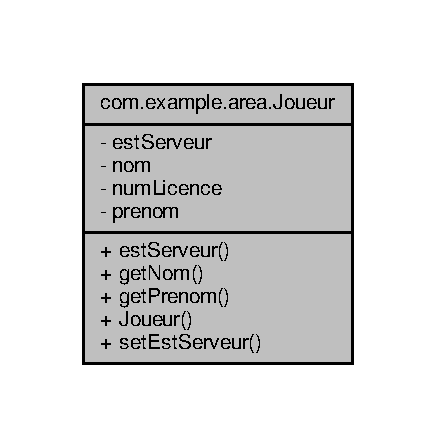
\includegraphics[width=209pt]{classcom_1_1example_1_1area_1_1_joueur__coll__graph}
\end{center}
\end{figure}
\subsubsection*{Fonctions membres publiques}
\begin{DoxyCompactItemize}
\item 
boolean \hyperlink{classcom_1_1example_1_1area_1_1_joueur_ad35bff2a14331bada30ccc164d25f50f}{est\+Serveur} ()
\begin{DoxyCompactList}\small\item\em Accesseur de l\textquotesingle{}attribut est\+Serveur. \end{DoxyCompactList}\item 
String \hyperlink{classcom_1_1example_1_1area_1_1_joueur_a4e43a9187363501204af7b2f2c84a9a4}{get\+Nom} ()
\begin{DoxyCompactList}\small\item\em Accesseur de l\textquotesingle{}attribut nom. \end{DoxyCompactList}\item 
String \hyperlink{classcom_1_1example_1_1area_1_1_joueur_ac2cd099ccfc34c48fbabde5649514a27}{get\+Prenom} ()
\begin{DoxyCompactList}\small\item\em Accesseur de l\textquotesingle{}attribut prenom. \end{DoxyCompactList}\item 
\hyperlink{classcom_1_1example_1_1area_1_1_joueur_a62953f37425da88ba6e6e2426ab67afc}{Joueur} (String \hyperlink{classcom_1_1example_1_1area_1_1_joueur_a98dde75942f6a48d9acf0abb67742dc3}{nom}, String \hyperlink{classcom_1_1example_1_1area_1_1_joueur_a9a49f14719dfc48cf557ef8677e2b2bc}{prenom}, int \hyperlink{classcom_1_1example_1_1area_1_1_joueur_a559bd07d0a47e8fc1ec3050890f00589}{num\+Licence})
\item 
void \hyperlink{classcom_1_1example_1_1area_1_1_joueur_aa0ae3b52616cc034cd6270eade9a1be7}{set\+Est\+Serveur} (boolean \hyperlink{classcom_1_1example_1_1area_1_1_joueur_abbc3e85c6740569af7f1bd2cb7aad6a2}{est\+Serveur})
\begin{DoxyCompactList}\small\item\em Mutateur de l\textquotesingle{}attribut est\+Serveur. \end{DoxyCompactList}\end{DoxyCompactItemize}
\subsubsection*{Attributs privés}
\begin{DoxyCompactItemize}
\item 
boolean \hyperlink{classcom_1_1example_1_1area_1_1_joueur_abbc3e85c6740569af7f1bd2cb7aad6a2}{est\+Serveur}
\item 
String \hyperlink{classcom_1_1example_1_1area_1_1_joueur_a98dde75942f6a48d9acf0abb67742dc3}{nom}
\item 
int \hyperlink{classcom_1_1example_1_1area_1_1_joueur_a559bd07d0a47e8fc1ec3050890f00589}{num\+Licence}
\item 
String \hyperlink{classcom_1_1example_1_1area_1_1_joueur_a9a49f14719dfc48cf557ef8677e2b2bc}{prenom}
\end{DoxyCompactItemize}


\subsubsection{Description détaillée}
Classe regroupant les informations d\textquotesingle{}un joueur. 

Définition à la ligne \hyperlink{_joueur_8java_source_l00018}{18} du fichier \hyperlink{_joueur_8java_source}{Joueur.\+java}.



\subsubsection{Documentation des constructeurs et destructeur}
\mbox{\Hypertarget{classcom_1_1example_1_1area_1_1_joueur_a62953f37425da88ba6e6e2426ab67afc}\label{classcom_1_1example_1_1area_1_1_joueur_a62953f37425da88ba6e6e2426ab67afc}} 
\index{com\+::example\+::area\+::\+Joueur@{com\+::example\+::area\+::\+Joueur}!Joueur@{Joueur}}
\index{Joueur@{Joueur}!com\+::example\+::area\+::\+Joueur@{com\+::example\+::area\+::\+Joueur}}
\paragraph{\texorpdfstring{Joueur()}{Joueur()}}
{\footnotesize\ttfamily com.\+example.\+area.\+Joueur.\+Joueur (\begin{DoxyParamCaption}\item[{String}]{nom,  }\item[{String}]{prenom,  }\item[{int}]{num\+Licence }\end{DoxyParamCaption})}



Définition à la ligne \hyperlink{_joueur_8java_source_l00028}{28} du fichier \hyperlink{_joueur_8java_source}{Joueur.\+java}.



Références \hyperlink{_joueur_8java_source_l00023}{com.\+example.\+area.\+Joueur.\+nom}, \hyperlink{_joueur_8java_source_l00025}{com.\+example.\+area.\+Joueur.\+num\+Licence}, et \hyperlink{_joueur_8java_source_l00024}{com.\+example.\+area.\+Joueur.\+prenom}.


\begin{DoxyCode}
00029       \{
00030           this.\hyperlink{classcom_1_1example_1_1area_1_1_joueur_a98dde75942f6a48d9acf0abb67742dc3}{nom} = \hyperlink{classcom_1_1example_1_1area_1_1_joueur_a98dde75942f6a48d9acf0abb67742dc3}{nom};
00031           this.\hyperlink{classcom_1_1example_1_1area_1_1_joueur_a9a49f14719dfc48cf557ef8677e2b2bc}{prenom} = \hyperlink{classcom_1_1example_1_1area_1_1_joueur_a9a49f14719dfc48cf557ef8677e2b2bc}{prenom};
00032           this.\hyperlink{classcom_1_1example_1_1area_1_1_joueur_a559bd07d0a47e8fc1ec3050890f00589}{numLicence} = \hyperlink{classcom_1_1example_1_1area_1_1_joueur_a559bd07d0a47e8fc1ec3050890f00589}{numLicence};
00033           this.\hyperlink{classcom_1_1example_1_1area_1_1_joueur_ad35bff2a14331bada30ccc164d25f50f}{estServeur} = \textcolor{keyword}{false};
00034       \}
\end{DoxyCode}


\subsubsection{Documentation des fonctions membres}
\mbox{\Hypertarget{classcom_1_1example_1_1area_1_1_joueur_ad35bff2a14331bada30ccc164d25f50f}\label{classcom_1_1example_1_1area_1_1_joueur_ad35bff2a14331bada30ccc164d25f50f}} 
\index{com\+::example\+::area\+::\+Joueur@{com\+::example\+::area\+::\+Joueur}!est\+Serveur@{est\+Serveur}}
\index{est\+Serveur@{est\+Serveur}!com\+::example\+::area\+::\+Joueur@{com\+::example\+::area\+::\+Joueur}}
\paragraph{\texorpdfstring{est\+Serveur()}{estServeur()}}
{\footnotesize\ttfamily boolean com.\+example.\+area.\+Joueur.\+est\+Serveur (\begin{DoxyParamCaption}{ }\end{DoxyParamCaption})}



Accesseur de l\textquotesingle{}attribut est\+Serveur. 



Définition à la ligne \hyperlink{_joueur_8java_source_l00055}{55} du fichier \hyperlink{_joueur_8java_source}{Joueur.\+java}.



Référencé par \hyperlink{_joueur_8java_source_l00063}{com.\+example.\+area.\+Joueur.\+set\+Est\+Serveur()}.


\begin{DoxyCode}
00056       \{
00057           \textcolor{keywordflow}{return} \hyperlink{classcom_1_1example_1_1area_1_1_joueur_ad35bff2a14331bada30ccc164d25f50f}{estServeur};
00058       \}
\end{DoxyCode}
\mbox{\Hypertarget{classcom_1_1example_1_1area_1_1_joueur_a4e43a9187363501204af7b2f2c84a9a4}\label{classcom_1_1example_1_1area_1_1_joueur_a4e43a9187363501204af7b2f2c84a9a4}} 
\index{com\+::example\+::area\+::\+Joueur@{com\+::example\+::area\+::\+Joueur}!get\+Nom@{get\+Nom}}
\index{get\+Nom@{get\+Nom}!com\+::example\+::area\+::\+Joueur@{com\+::example\+::area\+::\+Joueur}}
\paragraph{\texorpdfstring{get\+Nom()}{getNom()}}
{\footnotesize\ttfamily String com.\+example.\+area.\+Joueur.\+get\+Nom (\begin{DoxyParamCaption}{ }\end{DoxyParamCaption})}



Accesseur de l\textquotesingle{}attribut nom. 



Définition à la ligne \hyperlink{_joueur_8java_source_l00039}{39} du fichier \hyperlink{_joueur_8java_source}{Joueur.\+java}.



Références \hyperlink{_joueur_8java_source_l00023}{com.\+example.\+area.\+Joueur.\+nom}.



Référencé par \hyperlink{_i_h_m_gestion_partie_8java_source_l00447}{com.\+example.\+area.\+I\+H\+M\+Gestion\+Partie.\+afficher\+Serveur()}, \hyperlink{_i_h_m_gestion_rencontre_8java_source_l00343}{com.\+example.\+area.\+I\+H\+M\+Gestion\+Rencontre.\+formater\+Partie()}, \hyperlink{_partie_8java_source_l00334}{com.\+example.\+area.\+Partie.\+get\+Serveur()}, et \hyperlink{_i_h_m_gestion_rencontre_8java_source_l00281}{com.\+example.\+area.\+I\+H\+M\+Gestion\+Rencontre.\+recuperer\+Noms\+Joueurs()}.


\begin{DoxyCode}
00040       \{
00041           \textcolor{keywordflow}{return} \hyperlink{classcom_1_1example_1_1area_1_1_joueur_a98dde75942f6a48d9acf0abb67742dc3}{nom};
00042       \}
\end{DoxyCode}
\mbox{\Hypertarget{classcom_1_1example_1_1area_1_1_joueur_ac2cd099ccfc34c48fbabde5649514a27}\label{classcom_1_1example_1_1area_1_1_joueur_ac2cd099ccfc34c48fbabde5649514a27}} 
\index{com\+::example\+::area\+::\+Joueur@{com\+::example\+::area\+::\+Joueur}!get\+Prenom@{get\+Prenom}}
\index{get\+Prenom@{get\+Prenom}!com\+::example\+::area\+::\+Joueur@{com\+::example\+::area\+::\+Joueur}}
\paragraph{\texorpdfstring{get\+Prenom()}{getPrenom()}}
{\footnotesize\ttfamily String com.\+example.\+area.\+Joueur.\+get\+Prenom (\begin{DoxyParamCaption}{ }\end{DoxyParamCaption})}



Accesseur de l\textquotesingle{}attribut prenom. 



Définition à la ligne \hyperlink{_joueur_8java_source_l00047}{47} du fichier \hyperlink{_joueur_8java_source}{Joueur.\+java}.



Références \hyperlink{_joueur_8java_source_l00024}{com.\+example.\+area.\+Joueur.\+prenom}.



Référencé par \hyperlink{_i_h_m_gestion_partie_8java_source_l00447}{com.\+example.\+area.\+I\+H\+M\+Gestion\+Partie.\+afficher\+Serveur()}, \hyperlink{_i_h_m_gestion_rencontre_8java_source_l00343}{com.\+example.\+area.\+I\+H\+M\+Gestion\+Rencontre.\+formater\+Partie()}, \hyperlink{_partie_8java_source_l00334}{com.\+example.\+area.\+Partie.\+get\+Serveur()}, et \hyperlink{_i_h_m_gestion_rencontre_8java_source_l00281}{com.\+example.\+area.\+I\+H\+M\+Gestion\+Rencontre.\+recuperer\+Noms\+Joueurs()}.


\begin{DoxyCode}
00048       \{
00049           \textcolor{keywordflow}{return} \hyperlink{classcom_1_1example_1_1area_1_1_joueur_a9a49f14719dfc48cf557ef8677e2b2bc}{prenom};
00050       \}
\end{DoxyCode}
\mbox{\Hypertarget{classcom_1_1example_1_1area_1_1_joueur_aa0ae3b52616cc034cd6270eade9a1be7}\label{classcom_1_1example_1_1area_1_1_joueur_aa0ae3b52616cc034cd6270eade9a1be7}} 
\index{com\+::example\+::area\+::\+Joueur@{com\+::example\+::area\+::\+Joueur}!set\+Est\+Serveur@{set\+Est\+Serveur}}
\index{set\+Est\+Serveur@{set\+Est\+Serveur}!com\+::example\+::area\+::\+Joueur@{com\+::example\+::area\+::\+Joueur}}
\paragraph{\texorpdfstring{set\+Est\+Serveur()}{setEstServeur()}}
{\footnotesize\ttfamily void com.\+example.\+area.\+Joueur.\+set\+Est\+Serveur (\begin{DoxyParamCaption}\item[{boolean}]{est\+Serveur }\end{DoxyParamCaption})}



Mutateur de l\textquotesingle{}attribut est\+Serveur. 



Définition à la ligne \hyperlink{_joueur_8java_source_l00063}{63} du fichier \hyperlink{_joueur_8java_source}{Joueur.\+java}.



Références \hyperlink{_joueur_8java_source_l00055}{com.\+example.\+area.\+Joueur.\+est\+Serveur()}.



Référencé par \hyperlink{_partie_8java_source_l00293}{com.\+example.\+area.\+Partie.\+permuter\+Serveur\+Relanceur\+Duo()}.


\begin{DoxyCode}
00064     \{
00065         this.\hyperlink{classcom_1_1example_1_1area_1_1_joueur_ad35bff2a14331bada30ccc164d25f50f}{estServeur} = \hyperlink{classcom_1_1example_1_1area_1_1_joueur_ad35bff2a14331bada30ccc164d25f50f}{estServeur};
00066     \}
\end{DoxyCode}


\subsubsection{Documentation des données membres}
\mbox{\Hypertarget{classcom_1_1example_1_1area_1_1_joueur_abbc3e85c6740569af7f1bd2cb7aad6a2}\label{classcom_1_1example_1_1area_1_1_joueur_abbc3e85c6740569af7f1bd2cb7aad6a2}} 
\index{com\+::example\+::area\+::\+Joueur@{com\+::example\+::area\+::\+Joueur}!est\+Serveur@{est\+Serveur}}
\index{est\+Serveur@{est\+Serveur}!com\+::example\+::area\+::\+Joueur@{com\+::example\+::area\+::\+Joueur}}
\paragraph{\texorpdfstring{est\+Serveur}{estServeur}}
{\footnotesize\ttfamily boolean com.\+example.\+area.\+Joueur.\+est\+Serveur\hspace{0.3cm}{\ttfamily [private]}}



Définition à la ligne \hyperlink{_joueur_8java_source_l00026}{26} du fichier \hyperlink{_joueur_8java_source}{Joueur.\+java}.



Référencé par \hyperlink{_partie_8java_source_l00315}{com.\+example.\+area.\+Partie.\+trouver\+Serveur()}.

\mbox{\Hypertarget{classcom_1_1example_1_1area_1_1_joueur_a98dde75942f6a48d9acf0abb67742dc3}\label{classcom_1_1example_1_1area_1_1_joueur_a98dde75942f6a48d9acf0abb67742dc3}} 
\index{com\+::example\+::area\+::\+Joueur@{com\+::example\+::area\+::\+Joueur}!nom@{nom}}
\index{nom@{nom}!com\+::example\+::area\+::\+Joueur@{com\+::example\+::area\+::\+Joueur}}
\paragraph{\texorpdfstring{nom}{nom}}
{\footnotesize\ttfamily String com.\+example.\+area.\+Joueur.\+nom\hspace{0.3cm}{\ttfamily [private]}}

Attributs 

Définition à la ligne \hyperlink{_joueur_8java_source_l00023}{23} du fichier \hyperlink{_joueur_8java_source}{Joueur.\+java}.



Référencé par \hyperlink{_joueur_8java_source_l00039}{com.\+example.\+area.\+Joueur.\+get\+Nom()}, et \hyperlink{_joueur_8java_source_l00028}{com.\+example.\+area.\+Joueur.\+Joueur()}.

\mbox{\Hypertarget{classcom_1_1example_1_1area_1_1_joueur_a559bd07d0a47e8fc1ec3050890f00589}\label{classcom_1_1example_1_1area_1_1_joueur_a559bd07d0a47e8fc1ec3050890f00589}} 
\index{com\+::example\+::area\+::\+Joueur@{com\+::example\+::area\+::\+Joueur}!num\+Licence@{num\+Licence}}
\index{num\+Licence@{num\+Licence}!com\+::example\+::area\+::\+Joueur@{com\+::example\+::area\+::\+Joueur}}
\paragraph{\texorpdfstring{num\+Licence}{numLicence}}
{\footnotesize\ttfamily int com.\+example.\+area.\+Joueur.\+num\+Licence\hspace{0.3cm}{\ttfamily [private]}}



Définition à la ligne \hyperlink{_joueur_8java_source_l00025}{25} du fichier \hyperlink{_joueur_8java_source}{Joueur.\+java}.



Référencé par \hyperlink{_joueur_8java_source_l00028}{com.\+example.\+area.\+Joueur.\+Joueur()}.

\mbox{\Hypertarget{classcom_1_1example_1_1area_1_1_joueur_a9a49f14719dfc48cf557ef8677e2b2bc}\label{classcom_1_1example_1_1area_1_1_joueur_a9a49f14719dfc48cf557ef8677e2b2bc}} 
\index{com\+::example\+::area\+::\+Joueur@{com\+::example\+::area\+::\+Joueur}!prenom@{prenom}}
\index{prenom@{prenom}!com\+::example\+::area\+::\+Joueur@{com\+::example\+::area\+::\+Joueur}}
\paragraph{\texorpdfstring{prenom}{prenom}}
{\footnotesize\ttfamily String com.\+example.\+area.\+Joueur.\+prenom\hspace{0.3cm}{\ttfamily [private]}}



Définition à la ligne \hyperlink{_joueur_8java_source_l00024}{24} du fichier \hyperlink{_joueur_8java_source}{Joueur.\+java}.



Référencé par \hyperlink{_joueur_8java_source_l00047}{com.\+example.\+area.\+Joueur.\+get\+Prenom()}, et \hyperlink{_joueur_8java_source_l00028}{com.\+example.\+area.\+Joueur.\+Joueur()}.



La documentation de cette classe a été générée à partir du fichier suivant \+:\begin{DoxyCompactItemize}
\item 
\hyperlink{_joueur_8java}{Joueur.\+java}\end{DoxyCompactItemize}

\hypertarget{classcom_1_1example_1_1area_1_1_liaison_bluetooth}{}\subsection{Référence de la classe com.\+example.\+area.\+Liaison\+Bluetooth}
\label{classcom_1_1example_1_1area_1_1_liaison_bluetooth}\index{com.\+example.\+area.\+Liaison\+Bluetooth@{com.\+example.\+area.\+Liaison\+Bluetooth}}


Permet de gérer la communication bluetooth.  




Graphe de collaboration de com.\+example.\+area.\+Liaison\+Bluetooth\+:
\nopagebreak
\begin{figure}[H]
\begin{center}
\leavevmode
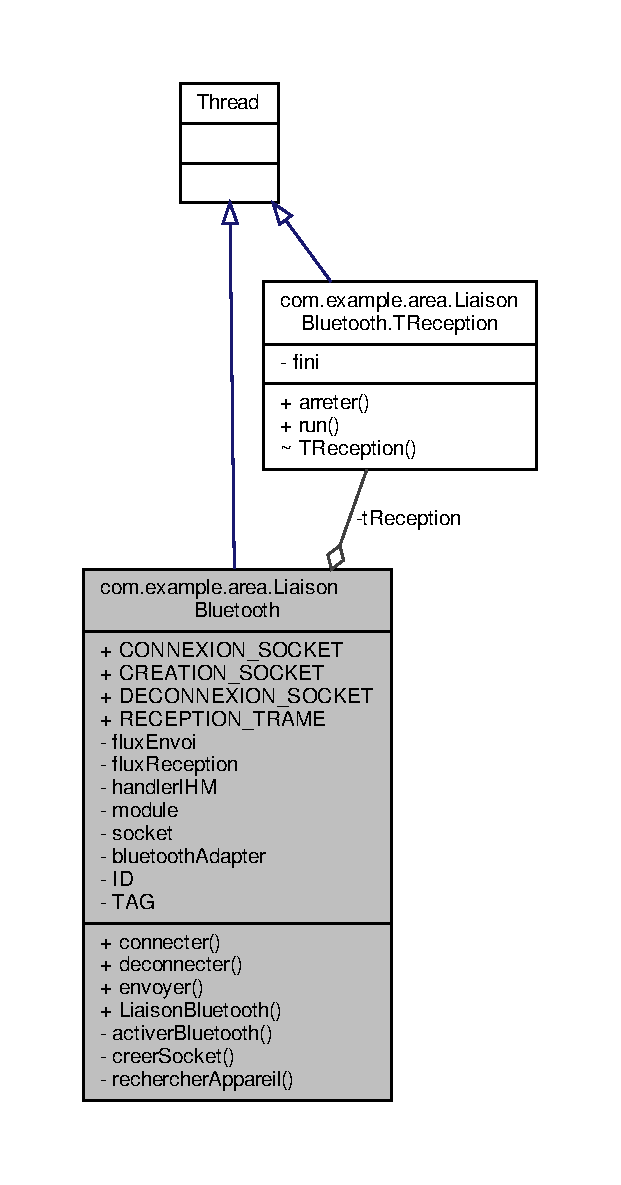
\includegraphics[height=550pt]{classcom_1_1example_1_1area_1_1_liaison_bluetooth__coll__graph}
\end{center}
\end{figure}
\subsubsection*{Classes}
\begin{DoxyCompactItemize}
\item 
class \hyperlink{classcom_1_1example_1_1area_1_1_liaison_bluetooth_1_1_t_reception}{T\+Reception}
\end{DoxyCompactItemize}
\subsubsection*{Fonctions membres publiques}
\begin{DoxyCompactItemize}
\item 
void \hyperlink{classcom_1_1example_1_1area_1_1_liaison_bluetooth_a7b9662a4224762b23c814d1f4539002a}{connecter} ()
\begin{DoxyCompactList}\small\item\em Méthode pour ouvrir la connexion avec un appareil. \end{DoxyCompactList}\item 
void \hyperlink{classcom_1_1example_1_1area_1_1_liaison_bluetooth_a10b356586feed95ecacb0a57cb51f0e6}{deconnecter} ()
\begin{DoxyCompactList}\small\item\em Méthode pour fermer la connexion avec un appareil. \end{DoxyCompactList}\item 
void \hyperlink{classcom_1_1example_1_1area_1_1_liaison_bluetooth_a67360b2f673b47b8a552a9e789a93fce}{envoyer} (String donnees)
\begin{DoxyCompactList}\small\item\em Méthode pour envoyer des données. \end{DoxyCompactList}\item 
\hyperlink{classcom_1_1example_1_1area_1_1_liaison_bluetooth_a1388dcaf09e2493d2fac6ddb9d8d58e1}{Liaison\+Bluetooth} (String nom\+Appareil, String adresse\+Appareil, Handler \hyperlink{classcom_1_1example_1_1area_1_1_liaison_bluetooth_ace2c20759fc96d3ae787f1f726fd2691}{handler\+I\+HM})
\end{DoxyCompactItemize}
\subsubsection*{Attributs publics statiques}
\begin{DoxyCompactItemize}
\item 
static final int \hyperlink{classcom_1_1example_1_1area_1_1_liaison_bluetooth_a4870b4fac5c0f1aedac1bb40346d43da}{C\+O\+N\+N\+E\+X\+I\+O\+N\+\_\+\+S\+O\+C\+K\+ET} = 2
\item 
static final int \hyperlink{classcom_1_1example_1_1area_1_1_liaison_bluetooth_ac961c73879bd0de9933b2fc310cc5e7e}{C\+R\+E\+A\+T\+I\+O\+N\+\_\+\+S\+O\+C\+K\+ET} = 1
\item 
static final int \hyperlink{classcom_1_1example_1_1area_1_1_liaison_bluetooth_a8ff08468d7b2cead9c3714c665f75d0e}{D\+E\+C\+O\+N\+N\+E\+X\+I\+O\+N\+\_\+\+S\+O\+C\+K\+ET} = 3
\item 
static final int \hyperlink{classcom_1_1example_1_1area_1_1_liaison_bluetooth_a1a3058c683cec15fe0f3699f7fc26073}{R\+E\+C\+E\+P\+T\+I\+O\+N\+\_\+\+T\+R\+A\+ME} = 4
\end{DoxyCompactItemize}
\subsubsection*{Fonctions membres privées}
\begin{DoxyCompactItemize}
\item 
void \hyperlink{classcom_1_1example_1_1area_1_1_liaison_bluetooth_acc6b0431535ca4d7abc65e84deff8002}{activer\+Bluetooth} ()
\begin{DoxyCompactList}\small\item\em Méthode permettant d\textquotesingle{}activer le bluetooth s\textquotesingle{}il ne l\textquotesingle{}est pas. \end{DoxyCompactList}\item 
boolean \hyperlink{classcom_1_1example_1_1area_1_1_liaison_bluetooth_a69ea46dca5a0690d5d8231731ae60d9f}{creer\+Socket} ()
\begin{DoxyCompactList}\small\item\em Méthode permettant de créer une socket à partir d\textquotesingle{}un appareil. \end{DoxyCompactList}\item 
boolean \hyperlink{classcom_1_1example_1_1area_1_1_liaison_bluetooth_a47786b43e054a81e08356cd22b4cb37e}{rechercher\+Appareil} (String id\+Appareil)
\begin{DoxyCompactList}\small\item\em Méthode permettant de rechercher un appareil à partir d\textquotesingle{}une adresse. \end{DoxyCompactList}\end{DoxyCompactItemize}
\subsubsection*{Attributs privés}
\begin{DoxyCompactItemize}
\item 
Output\+Stream \hyperlink{classcom_1_1example_1_1area_1_1_liaison_bluetooth_ab6b076591203cae95fde933717019c5d}{flux\+Envoi} = null
\item 
Input\+Stream \hyperlink{classcom_1_1example_1_1area_1_1_liaison_bluetooth_a9a3a7d77bae06a972782b6e73471878d}{flux\+Reception} = null
\item 
Handler \hyperlink{classcom_1_1example_1_1area_1_1_liaison_bluetooth_ace2c20759fc96d3ae787f1f726fd2691}{handler\+I\+HM} = null
\item 
Bluetooth\+Device \hyperlink{classcom_1_1example_1_1area_1_1_liaison_bluetooth_a80068a7178f6c84eae7bab50cf0a784a}{module} = null
\item 
Bluetooth\+Socket \hyperlink{classcom_1_1example_1_1area_1_1_liaison_bluetooth_ab59b57f5e59d0236e49ecf68c053cb27}{socket} = null
\item 
\hyperlink{classcom_1_1example_1_1area_1_1_liaison_bluetooth_1_1_t_reception}{T\+Reception} \hyperlink{classcom_1_1example_1_1area_1_1_liaison_bluetooth_ae3ef79eced8ab42b066b624108860d48}{t\+Reception} = null
\end{DoxyCompactItemize}
\subsubsection*{Attributs privés statiques}
\begin{DoxyCompactItemize}
\item 
static Bluetooth\+Adapter \hyperlink{classcom_1_1example_1_1area_1_1_liaison_bluetooth_a7462ce946676c47ee83289c7bb436b64}{bluetooth\+Adapter} = null
\item 
static final String \hyperlink{classcom_1_1example_1_1area_1_1_liaison_bluetooth_a8f4d17b8ac09c7ba9213163de86fb669}{ID} = \char`\"{}00001101-\/0000-\/1000-\/8000-\/00805\+F9\+B34\+F\+B\char`\"{}
\item 
static final String \hyperlink{classcom_1_1example_1_1area_1_1_liaison_bluetooth_ac51aa4b63fae5c36734a061cc05d7fc9}{T\+AG} = \char`\"{}\+\_\+\+Liaison\+Bluetooth\char`\"{}
\end{DoxyCompactItemize}


\subsubsection{Description détaillée}
Permet de gérer la communication bluetooth. 

Définition à la ligne \hyperlink{_liaison_bluetooth_8java_source_l00031}{31} du fichier \hyperlink{_liaison_bluetooth_8java_source}{Liaison\+Bluetooth.\+java}.



\subsubsection{Documentation des constructeurs et destructeur}
\mbox{\Hypertarget{classcom_1_1example_1_1area_1_1_liaison_bluetooth_a1388dcaf09e2493d2fac6ddb9d8d58e1}\label{classcom_1_1example_1_1area_1_1_liaison_bluetooth_a1388dcaf09e2493d2fac6ddb9d8d58e1}} 
\index{com\+::example\+::area\+::\+Liaison\+Bluetooth@{com\+::example\+::area\+::\+Liaison\+Bluetooth}!Liaison\+Bluetooth@{Liaison\+Bluetooth}}
\index{Liaison\+Bluetooth@{Liaison\+Bluetooth}!com\+::example\+::area\+::\+Liaison\+Bluetooth@{com\+::example\+::area\+::\+Liaison\+Bluetooth}}
\paragraph{\texorpdfstring{Liaison\+Bluetooth()}{LiaisonBluetooth()}}
{\footnotesize\ttfamily com.\+example.\+area.\+Liaison\+Bluetooth.\+Liaison\+Bluetooth (\begin{DoxyParamCaption}\item[{String}]{nom\+Appareil,  }\item[{String}]{adresse\+Appareil,  }\item[{Handler}]{handler\+I\+HM }\end{DoxyParamCaption})}



Définition à la ligne \hyperlink{_liaison_bluetooth_8java_source_l00048}{48} du fichier \hyperlink{_liaison_bluetooth_8java_source}{Liaison\+Bluetooth.\+java}.



Références \hyperlink{_liaison_bluetooth_8java_source_l00067}{com.\+example.\+area.\+Liaison\+Bluetooth.\+activer\+Bluetooth()}, \hyperlink{_liaison_bluetooth_8java_source_l00102}{com.\+example.\+area.\+Liaison\+Bluetooth.\+creer\+Socket()}, \hyperlink{_liaison_bluetooth_8java_source_l00046}{com.\+example.\+area.\+Liaison\+Bluetooth.\+handler\+I\+HM}, et \hyperlink{_liaison_bluetooth_8java_source_l00081}{com.\+example.\+area.\+Liaison\+Bluetooth.\+rechercher\+Appareil()}.


\begin{DoxyCode}
00049     \{
00050         this.\hyperlink{classcom_1_1example_1_1area_1_1_liaison_bluetooth_ace2c20759fc96d3ae787f1f726fd2691}{handlerIHM} = \hyperlink{classcom_1_1example_1_1area_1_1_liaison_bluetooth_ace2c20759fc96d3ae787f1f726fd2691}{handlerIHM};
00051 
00052         \hyperlink{classcom_1_1example_1_1area_1_1_liaison_bluetooth_acc6b0431535ca4d7abc65e84deff8002}{activerBluetooth}();
00053 
00054         \textcolor{keywordflow}{if}(\hyperlink{classcom_1_1example_1_1area_1_1_liaison_bluetooth_a47786b43e054a81e08356cd22b4cb37e}{rechercherAppareil}(nomAppareil))
00055         \{
00056             \hyperlink{classcom_1_1example_1_1area_1_1_liaison_bluetooth_a69ea46dca5a0690d5d8231731ae60d9f}{creerSocket}();
00057         \}
00058         \textcolor{keywordflow}{else} \textcolor{keywordflow}{if}(\hyperlink{classcom_1_1example_1_1area_1_1_liaison_bluetooth_a47786b43e054a81e08356cd22b4cb37e}{rechercherAppareil}(adresseAppareil))
00059         \{
00060             \hyperlink{classcom_1_1example_1_1area_1_1_liaison_bluetooth_a69ea46dca5a0690d5d8231731ae60d9f}{creerSocket}();
00061         \}
00062     \}
\end{DoxyCode}


\subsubsection{Documentation des fonctions membres}
\mbox{\Hypertarget{classcom_1_1example_1_1area_1_1_liaison_bluetooth_acc6b0431535ca4d7abc65e84deff8002}\label{classcom_1_1example_1_1area_1_1_liaison_bluetooth_acc6b0431535ca4d7abc65e84deff8002}} 
\index{com\+::example\+::area\+::\+Liaison\+Bluetooth@{com\+::example\+::area\+::\+Liaison\+Bluetooth}!activer\+Bluetooth@{activer\+Bluetooth}}
\index{activer\+Bluetooth@{activer\+Bluetooth}!com\+::example\+::area\+::\+Liaison\+Bluetooth@{com\+::example\+::area\+::\+Liaison\+Bluetooth}}
\paragraph{\texorpdfstring{activer\+Bluetooth()}{activerBluetooth()}}
{\footnotesize\ttfamily void com.\+example.\+area.\+Liaison\+Bluetooth.\+activer\+Bluetooth (\begin{DoxyParamCaption}{ }\end{DoxyParamCaption})\hspace{0.3cm}{\ttfamily [private]}}



Méthode permettant d\textquotesingle{}activer le bluetooth s\textquotesingle{}il ne l\textquotesingle{}est pas. 



Définition à la ligne \hyperlink{_liaison_bluetooth_8java_source_l00067}{67} du fichier \hyperlink{_liaison_bluetooth_8java_source}{Liaison\+Bluetooth.\+java}.



Référencé par \hyperlink{_liaison_bluetooth_8java_source_l00048}{com.\+example.\+area.\+Liaison\+Bluetooth.\+Liaison\+Bluetooth()}.


\begin{DoxyCode}
00068     \{
00069         \hyperlink{classcom_1_1example_1_1area_1_1_liaison_bluetooth_a7462ce946676c47ee83289c7bb436b64}{bluetoothAdapter} = BluetoothAdapter.getDefaultAdapter();
00070         \textcolor{keywordflow}{if} (!\hyperlink{classcom_1_1example_1_1area_1_1_liaison_bluetooth_a7462ce946676c47ee83289c7bb436b64}{bluetoothAdapter}.isEnabled())
00071         \{
00072             Log.d(\hyperlink{classcom_1_1example_1_1area_1_1_liaison_bluetooth_ac51aa4b63fae5c36734a061cc05d7fc9}{TAG},\textcolor{stringliteral}{"Activation du Bluetooth"});
00073             \hyperlink{classcom_1_1example_1_1area_1_1_liaison_bluetooth_a7462ce946676c47ee83289c7bb436b64}{bluetoothAdapter}.enable();
00074         \}
00075     \}
\end{DoxyCode}
\mbox{\Hypertarget{classcom_1_1example_1_1area_1_1_liaison_bluetooth_a7b9662a4224762b23c814d1f4539002a}\label{classcom_1_1example_1_1area_1_1_liaison_bluetooth_a7b9662a4224762b23c814d1f4539002a}} 
\index{com\+::example\+::area\+::\+Liaison\+Bluetooth@{com\+::example\+::area\+::\+Liaison\+Bluetooth}!connecter@{connecter}}
\index{connecter@{connecter}!com\+::example\+::area\+::\+Liaison\+Bluetooth@{com\+::example\+::area\+::\+Liaison\+Bluetooth}}
\paragraph{\texorpdfstring{connecter()}{connecter()}}
{\footnotesize\ttfamily void com.\+example.\+area.\+Liaison\+Bluetooth.\+connecter (\begin{DoxyParamCaption}{ }\end{DoxyParamCaption})}



Méthode pour ouvrir la connexion avec un appareil. 



Définition à la ligne \hyperlink{_liaison_bluetooth_8java_source_l00136}{136} du fichier \hyperlink{_liaison_bluetooth_8java_source}{Liaison\+Bluetooth.\+java}.



Références \hyperlink{_liaison_bluetooth_8java_source_l00036}{com.\+example.\+area.\+Liaison\+Bluetooth.\+C\+O\+N\+N\+E\+X\+I\+O\+N\+\_\+\+S\+O\+C\+K\+ET}.



Référencé par \hyperlink{_i_h_m_gestion_partie_8java_source_l00329}{com.\+example.\+area.\+I\+H\+M\+Gestion\+Partie.\+initialiser\+Liaison\+Bluetooth()}, et \hyperlink{_liaison_bluetooth_8java_source_l00240}{com.\+example.\+area.\+Liaison\+Bluetooth.\+T\+Reception.\+run()}.


\begin{DoxyCode}
00137     \{
00138         \textcolor{keywordflow}{if} (\hyperlink{classcom_1_1example_1_1area_1_1_liaison_bluetooth_a80068a7178f6c84eae7bab50cf0a784a}{module} == null || \hyperlink{classcom_1_1example_1_1area_1_1_liaison_bluetooth_ab59b57f5e59d0236e49ecf68c053cb27}{socket} == null)
00139             \textcolor{keywordflow}{return};
00140 
00141         Log.d(\hyperlink{classcom_1_1example_1_1area_1_1_liaison_bluetooth_ac51aa4b63fae5c36734a061cc05d7fc9}{TAG},\textcolor{stringliteral}{"Connexion au module "} + \hyperlink{classcom_1_1example_1_1area_1_1_liaison_bluetooth_a80068a7178f6c84eae7bab50cf0a784a}{module}.getName() + \textcolor{stringliteral}{" | Adresse : "} + 
      \hyperlink{classcom_1_1example_1_1area_1_1_liaison_bluetooth_a80068a7178f6c84eae7bab50cf0a784a}{module}.getAddress());
00142         \textcolor{keyword}{new} \hyperlink{class_thread}{Thread}()
00143         \{
00144             @Override \textcolor{keyword}{public} \textcolor{keywordtype}{void} run()
00145             \{
00146                 \textcolor{keywordflow}{try}
00147                 \{
00148                     \hyperlink{classcom_1_1example_1_1area_1_1_liaison_bluetooth_a7462ce946676c47ee83289c7bb436b64}{bluetoothAdapter}.cancelDiscovery();
00149                     \hyperlink{classcom_1_1example_1_1area_1_1_liaison_bluetooth_ab59b57f5e59d0236e49ecf68c053cb27}{socket}.connect();
00150                     \hyperlink{classcom_1_1example_1_1area_1_1_liaison_bluetooth_a9a3a7d77bae06a972782b6e73471878d}{fluxReception} = \hyperlink{classcom_1_1example_1_1area_1_1_liaison_bluetooth_ab59b57f5e59d0236e49ecf68c053cb27}{socket}.getInputStream();
00151                     \hyperlink{classcom_1_1example_1_1area_1_1_liaison_bluetooth_ab6b076591203cae95fde933717019c5d}{fluxEnvoi} = \hyperlink{classcom_1_1example_1_1area_1_1_liaison_bluetooth_ab59b57f5e59d0236e49ecf68c053cb27}{socket}.getOutputStream();
00152                     \textcolor{keywordflow}{if} (!\hyperlink{classcom_1_1example_1_1area_1_1_liaison_bluetooth_ae3ef79eced8ab42b066b624108860d48}{tReception}.isAlive())
00153                         \hyperlink{classcom_1_1example_1_1area_1_1_liaison_bluetooth_ae3ef79eced8ab42b066b624108860d48}{tReception}.start();
00154                     Message message = \textcolor{keyword}{new} Message();
00155                     message.what = \hyperlink{classcom_1_1example_1_1area_1_1_liaison_bluetooth_a4870b4fac5c0f1aedac1bb40346d43da}{CONNEXION\_SOCKET};
00156                     message.obj = \hyperlink{classcom_1_1example_1_1area_1_1_liaison_bluetooth_a80068a7178f6c84eae7bab50cf0a784a}{module}.getName();
00157                     \hyperlink{classcom_1_1example_1_1area_1_1_liaison_bluetooth_ace2c20759fc96d3ae787f1f726fd2691}{handlerIHM}.sendMessage(message);
00158                 \}
00159                 \textcolor{keywordflow}{catch} (IOException e)
00160                 \{
00161                     Log.e(\hyperlink{classcom_1_1example_1_1area_1_1_liaison_bluetooth_ac51aa4b63fae5c36734a061cc05d7fc9}{TAG},\textcolor{stringliteral}{"Erreur ouverture du socket"});
00162                     e.printStackTrace();
00163                 \}
00164             \}
00165         \}.start();
00166     \}
\end{DoxyCode}
\mbox{\Hypertarget{classcom_1_1example_1_1area_1_1_liaison_bluetooth_a69ea46dca5a0690d5d8231731ae60d9f}\label{classcom_1_1example_1_1area_1_1_liaison_bluetooth_a69ea46dca5a0690d5d8231731ae60d9f}} 
\index{com\+::example\+::area\+::\+Liaison\+Bluetooth@{com\+::example\+::area\+::\+Liaison\+Bluetooth}!creer\+Socket@{creer\+Socket}}
\index{creer\+Socket@{creer\+Socket}!com\+::example\+::area\+::\+Liaison\+Bluetooth@{com\+::example\+::area\+::\+Liaison\+Bluetooth}}
\paragraph{\texorpdfstring{creer\+Socket()}{creerSocket()}}
{\footnotesize\ttfamily boolean com.\+example.\+area.\+Liaison\+Bluetooth.\+creer\+Socket (\begin{DoxyParamCaption}{ }\end{DoxyParamCaption})\hspace{0.3cm}{\ttfamily [private]}}



Méthode permettant de créer une socket à partir d\textquotesingle{}un appareil. 



Définition à la ligne \hyperlink{_liaison_bluetooth_8java_source_l00102}{102} du fichier \hyperlink{_liaison_bluetooth_8java_source}{Liaison\+Bluetooth.\+java}.



Références \hyperlink{_liaison_bluetooth_8java_source_l00035}{com.\+example.\+area.\+Liaison\+Bluetooth.\+C\+R\+E\+A\+T\+I\+O\+N\+\_\+\+S\+O\+C\+K\+ET}.



Référencé par \hyperlink{_liaison_bluetooth_8java_source_l00048}{com.\+example.\+area.\+Liaison\+Bluetooth.\+Liaison\+Bluetooth()}.


\begin{DoxyCode}
00103     \{
00104         \textcolor{keywordflow}{if}(\hyperlink{classcom_1_1example_1_1area_1_1_liaison_bluetooth_a80068a7178f6c84eae7bab50cf0a784a}{module} == null)
00105             \textcolor{keywordflow}{return} \textcolor{keyword}{false};
00106 
00107         Log.d(\hyperlink{classcom_1_1example_1_1area_1_1_liaison_bluetooth_ac51aa4b63fae5c36734a061cc05d7fc9}{TAG},\textcolor{stringliteral}{"Création de la socket pour l'appareil : "} + \hyperlink{classcom_1_1example_1_1area_1_1_liaison_bluetooth_a80068a7178f6c84eae7bab50cf0a784a}{module}.getName() + \textcolor{stringliteral}{" | Adresse : "} 
      + \hyperlink{classcom_1_1example_1_1area_1_1_liaison_bluetooth_a80068a7178f6c84eae7bab50cf0a784a}{module}.getAddress());
00108         \textcolor{keywordflow}{try}
00109         \{
00110             \hyperlink{classcom_1_1example_1_1area_1_1_liaison_bluetooth_ab59b57f5e59d0236e49ecf68c053cb27}{socket} = \hyperlink{classcom_1_1example_1_1area_1_1_liaison_bluetooth_a80068a7178f6c84eae7bab50cf0a784a}{module}.createRfcommSocketToServiceRecord(UUID.fromString(
      \hyperlink{classcom_1_1example_1_1area_1_1_liaison_bluetooth_a8f4d17b8ac09c7ba9213163de86fb669}{ID}));
00111         \}
00112         \textcolor{keywordflow}{catch} (IOException e)
00113         \{
00114             e.printStackTrace();
00115             \hyperlink{classcom_1_1example_1_1area_1_1_liaison_bluetooth_ab59b57f5e59d0236e49ecf68c053cb27}{socket} = null;
00116             Log.d(\hyperlink{classcom_1_1example_1_1area_1_1_liaison_bluetooth_ac51aa4b63fae5c36734a061cc05d7fc9}{TAG}, \textcolor{stringliteral}{"Echec de la création de socket"});
00117             \textcolor{keywordflow}{return} \textcolor{keyword}{false};
00118         \}
00119 
00120         \textcolor{keywordflow}{if} (\hyperlink{classcom_1_1example_1_1area_1_1_liaison_bluetooth_ab59b57f5e59d0236e49ecf68c053cb27}{socket} != null)
00121         \{
00122             \hyperlink{classcom_1_1example_1_1area_1_1_liaison_bluetooth_ae3ef79eced8ab42b066b624108860d48}{tReception} = \textcolor{keyword}{new} TReception();
00123             Message message = \textcolor{keyword}{new} Message();
00124             message.what = \hyperlink{classcom_1_1example_1_1area_1_1_liaison_bluetooth_ac961c73879bd0de9933b2fc310cc5e7e}{CREATION\_SOCKET};
00125             message.obj = \hyperlink{classcom_1_1example_1_1area_1_1_liaison_bluetooth_a80068a7178f6c84eae7bab50cf0a784a}{module}.getName();
00126             \hyperlink{classcom_1_1example_1_1area_1_1_liaison_bluetooth_ace2c20759fc96d3ae787f1f726fd2691}{handlerIHM}.sendMessage(message);
00127             \textcolor{keywordflow}{return} \textcolor{keyword}{true};
00128         \}
00129 
00130         \textcolor{keywordflow}{return} \textcolor{keyword}{false};
00131     \}
\end{DoxyCode}
\mbox{\Hypertarget{classcom_1_1example_1_1area_1_1_liaison_bluetooth_a10b356586feed95ecacb0a57cb51f0e6}\label{classcom_1_1example_1_1area_1_1_liaison_bluetooth_a10b356586feed95ecacb0a57cb51f0e6}} 
\index{com\+::example\+::area\+::\+Liaison\+Bluetooth@{com\+::example\+::area\+::\+Liaison\+Bluetooth}!deconnecter@{deconnecter}}
\index{deconnecter@{deconnecter}!com\+::example\+::area\+::\+Liaison\+Bluetooth@{com\+::example\+::area\+::\+Liaison\+Bluetooth}}
\paragraph{\texorpdfstring{deconnecter()}{deconnecter()}}
{\footnotesize\ttfamily void com.\+example.\+area.\+Liaison\+Bluetooth.\+deconnecter (\begin{DoxyParamCaption}{ }\end{DoxyParamCaption})}



Méthode pour fermer la connexion avec un appareil. 



Définition à la ligne \hyperlink{_liaison_bluetooth_8java_source_l00171}{171} du fichier \hyperlink{_liaison_bluetooth_8java_source}{Liaison\+Bluetooth.\+java}.



Références \hyperlink{_liaison_bluetooth_8java_source_l00287}{com.\+example.\+area.\+Liaison\+Bluetooth.\+T\+Reception.\+arreter()}, et \hyperlink{_liaison_bluetooth_8java_source_l00037}{com.\+example.\+area.\+Liaison\+Bluetooth.\+D\+E\+C\+O\+N\+N\+E\+X\+I\+O\+N\+\_\+\+S\+O\+C\+K\+ET}.



Référencé par \hyperlink{_i_h_m_gestion_partie_8java_source_l00169}{com.\+example.\+area.\+I\+H\+M\+Gestion\+Partie.\+on\+Destroy()}.


\begin{DoxyCode}
00172     \{
00173         \textcolor{keywordflow}{if} (\hyperlink{classcom_1_1example_1_1area_1_1_liaison_bluetooth_a80068a7178f6c84eae7bab50cf0a784a}{module} == null || \hyperlink{classcom_1_1example_1_1area_1_1_liaison_bluetooth_ab59b57f5e59d0236e49ecf68c053cb27}{socket} == null)
00174             \textcolor{keywordflow}{return};
00175 
00176         Log.d(\hyperlink{classcom_1_1example_1_1area_1_1_liaison_bluetooth_ac51aa4b63fae5c36734a061cc05d7fc9}{TAG},\textcolor{stringliteral}{"Déconnexion du module "} + \hyperlink{classcom_1_1example_1_1area_1_1_liaison_bluetooth_a80068a7178f6c84eae7bab50cf0a784a}{module}.getName() + \textcolor{stringliteral}{" | Adresse : "} + 
      \hyperlink{classcom_1_1example_1_1area_1_1_liaison_bluetooth_a80068a7178f6c84eae7bab50cf0a784a}{module}.getAddress());
00177         \textcolor{keyword}{new} \hyperlink{class_thread}{Thread}()
00178         \{
00179             @Override \textcolor{keyword}{public} \textcolor{keywordtype}{void} run()
00180             \{
00181                 \textcolor{keywordflow}{try}
00182                 \{
00183                     \hyperlink{classcom_1_1example_1_1area_1_1_liaison_bluetooth_ae3ef79eced8ab42b066b624108860d48}{tReception}.\hyperlink{classcom_1_1example_1_1area_1_1_liaison_bluetooth_1_1_t_reception_a89f97f22a976b8632e82b2aa94ab2674}{arreter}();
00184                     \hyperlink{classcom_1_1example_1_1area_1_1_liaison_bluetooth_ab59b57f5e59d0236e49ecf68c053cb27}{socket}.close();
00185                     Message message = \textcolor{keyword}{new} Message();
00186                     message.what = \hyperlink{classcom_1_1example_1_1area_1_1_liaison_bluetooth_a8ff08468d7b2cead9c3714c665f75d0e}{DECONNEXION\_SOCKET};
00187                     message.obj = \hyperlink{classcom_1_1example_1_1area_1_1_liaison_bluetooth_a80068a7178f6c84eae7bab50cf0a784a}{module}.getName();
00188                     \hyperlink{classcom_1_1example_1_1area_1_1_liaison_bluetooth_ace2c20759fc96d3ae787f1f726fd2691}{handlerIHM}.sendMessage(message);
00189                 \}
00190                 \textcolor{keywordflow}{catch} (IOException e)
00191                 \{
00192                     Log.e(\hyperlink{classcom_1_1example_1_1area_1_1_liaison_bluetooth_ac51aa4b63fae5c36734a061cc05d7fc9}{TAG},\textcolor{stringliteral}{"Erreur fermeture du socket"});
00193                     e.printStackTrace();
00194                 \}
00195             \}
00196         \}.start();
00197     \}
\end{DoxyCode}
\mbox{\Hypertarget{classcom_1_1example_1_1area_1_1_liaison_bluetooth_a67360b2f673b47b8a552a9e789a93fce}\label{classcom_1_1example_1_1area_1_1_liaison_bluetooth_a67360b2f673b47b8a552a9e789a93fce}} 
\index{com\+::example\+::area\+::\+Liaison\+Bluetooth@{com\+::example\+::area\+::\+Liaison\+Bluetooth}!envoyer@{envoyer}}
\index{envoyer@{envoyer}!com\+::example\+::area\+::\+Liaison\+Bluetooth@{com\+::example\+::area\+::\+Liaison\+Bluetooth}}
\paragraph{\texorpdfstring{envoyer()}{envoyer()}}
{\footnotesize\ttfamily void com.\+example.\+area.\+Liaison\+Bluetooth.\+envoyer (\begin{DoxyParamCaption}\item[{String}]{donnees }\end{DoxyParamCaption})}



Méthode pour envoyer des données. 



Définition à la ligne \hyperlink{_liaison_bluetooth_8java_source_l00202}{202} du fichier \hyperlink{_liaison_bluetooth_8java_source}{Liaison\+Bluetooth.\+java}.



Référencé par \hyperlink{_i_h_m_gestion_partie_8java_source_l00346}{com.\+example.\+area.\+I\+H\+M\+Gestion\+Partie.\+connecter\+Boutons()}, \hyperlink{_i_h_m_gestion_partie_8java_source_l00291}{com.\+example.\+area.\+I\+H\+M\+Gestion\+Partie.\+initialiser\+Handler()}, et \hyperlink{_i_h_m_gestion_partie_8java_source_l00329}{com.\+example.\+area.\+I\+H\+M\+Gestion\+Partie.\+initialiser\+Liaison\+Bluetooth()}.


\begin{DoxyCode}
00203     \{
00204         \textcolor{keywordflow}{if} (\hyperlink{classcom_1_1example_1_1area_1_1_liaison_bluetooth_a80068a7178f6c84eae7bab50cf0a784a}{module} == null || \hyperlink{classcom_1_1example_1_1area_1_1_liaison_bluetooth_ab59b57f5e59d0236e49ecf68c053cb27}{socket} == null)
00205             \textcolor{keywordflow}{return};
00206 
00207         \textcolor{keyword}{new} \hyperlink{class_thread}{Thread}()
00208         \{
00209             @Override \textcolor{keyword}{public} \textcolor{keywordtype}{void} run()
00210             \{
00211                 \textcolor{keywordflow}{try}
00212                 \{
00213                     \textcolor{keywordflow}{if}(\hyperlink{classcom_1_1example_1_1area_1_1_liaison_bluetooth_ab59b57f5e59d0236e49ecf68c053cb27}{socket}.isConnected())
00214                     \{
00215                         Log.d(\hyperlink{classcom_1_1example_1_1area_1_1_liaison_bluetooth_ac51aa4b63fae5c36734a061cc05d7fc9}{TAG},\textcolor{stringliteral}{"Envoi vers le module "} + \hyperlink{classcom_1_1example_1_1area_1_1_liaison_bluetooth_a80068a7178f6c84eae7bab50cf0a784a}{module}.getName() + \textcolor{stringliteral}{" | Adresse : "} + 
      \hyperlink{classcom_1_1example_1_1area_1_1_liaison_bluetooth_a80068a7178f6c84eae7bab50cf0a784a}{module}.getAddress() + \textcolor{stringliteral}{" | Données : "} + donnees);
00216                         \hyperlink{classcom_1_1example_1_1area_1_1_liaison_bluetooth_ab6b076591203cae95fde933717019c5d}{fluxEnvoi}.write(donnees.getBytes());
00217                     \}
00218                 \}
00219                 \textcolor{keywordflow}{catch}(IOException e)
00220                 \{
00221                     Log.e(\hyperlink{classcom_1_1example_1_1area_1_1_liaison_bluetooth_ac51aa4b63fae5c36734a061cc05d7fc9}{TAG},\textcolor{stringliteral}{"Erreur envoi socket"});
00222                     e.printStackTrace();
00223                 \}
00224             \}
00225         \}.start();
00226     \}
\end{DoxyCode}
\mbox{\Hypertarget{classcom_1_1example_1_1area_1_1_liaison_bluetooth_a47786b43e054a81e08356cd22b4cb37e}\label{classcom_1_1example_1_1area_1_1_liaison_bluetooth_a47786b43e054a81e08356cd22b4cb37e}} 
\index{com\+::example\+::area\+::\+Liaison\+Bluetooth@{com\+::example\+::area\+::\+Liaison\+Bluetooth}!rechercher\+Appareil@{rechercher\+Appareil}}
\index{rechercher\+Appareil@{rechercher\+Appareil}!com\+::example\+::area\+::\+Liaison\+Bluetooth@{com\+::example\+::area\+::\+Liaison\+Bluetooth}}
\paragraph{\texorpdfstring{rechercher\+Appareil()}{rechercherAppareil()}}
{\footnotesize\ttfamily boolean com.\+example.\+area.\+Liaison\+Bluetooth.\+rechercher\+Appareil (\begin{DoxyParamCaption}\item[{String}]{id\+Appareil }\end{DoxyParamCaption})\hspace{0.3cm}{\ttfamily [private]}}



Méthode permettant de rechercher un appareil à partir d\textquotesingle{}une adresse. 


\begin{DoxyParams}{Paramètres}
{\em id\+Appareil} & Le nom ou l\textquotesingle{}adresse M\+AC du module Bluetooth à rechercher \\
\hline
\end{DoxyParams}


Définition à la ligne \hyperlink{_liaison_bluetooth_8java_source_l00081}{81} du fichier \hyperlink{_liaison_bluetooth_8java_source}{Liaison\+Bluetooth.\+java}.



Référencé par \hyperlink{_liaison_bluetooth_8java_source_l00048}{com.\+example.\+area.\+Liaison\+Bluetooth.\+Liaison\+Bluetooth()}.


\begin{DoxyCode}
00082     \{
00083         Set<BluetoothDevice> appareilsAppaires = \hyperlink{classcom_1_1example_1_1area_1_1_liaison_bluetooth_a7462ce946676c47ee83289c7bb436b64}{bluetoothAdapter}.getBondedDevices();
00084 
00085         Log.d(\hyperlink{classcom_1_1example_1_1area_1_1_liaison_bluetooth_ac51aa4b63fae5c36734a061cc05d7fc9}{TAG},\textcolor{stringliteral}{"Recherche l'appareil : "} + idAppareil);
00086         \textcolor{keywordflow}{for} (BluetoothDevice appareil : appareilsAppaires)
00087         \{
00088             Log.d(\hyperlink{classcom_1_1example_1_1area_1_1_liaison_bluetooth_ac51aa4b63fae5c36734a061cc05d7fc9}{TAG},\textcolor{stringliteral}{"Nom : "} + appareil.getName() + \textcolor{stringliteral}{" | Adresse : "} + appareil.getAddress());
00089             \textcolor{keywordflow}{if} (appareil.getAddress().equals(idAppareil) || appareil.getName().equals(idAppareil))
00090             \{
00091                 \hyperlink{classcom_1_1example_1_1area_1_1_liaison_bluetooth_a80068a7178f6c84eae7bab50cf0a784a}{module} = appareil;
00092                 \textcolor{keywordflow}{return} \textcolor{keyword}{true}; \textcolor{comment}{// trouvé !}
00093             \}
00094         \}
00095 
00096         \textcolor{keywordflow}{return} \textcolor{keyword}{false};
00097     \}
\end{DoxyCode}


\subsubsection{Documentation des données membres}
\mbox{\Hypertarget{classcom_1_1example_1_1area_1_1_liaison_bluetooth_a7462ce946676c47ee83289c7bb436b64}\label{classcom_1_1example_1_1area_1_1_liaison_bluetooth_a7462ce946676c47ee83289c7bb436b64}} 
\index{com\+::example\+::area\+::\+Liaison\+Bluetooth@{com\+::example\+::area\+::\+Liaison\+Bluetooth}!bluetooth\+Adapter@{bluetooth\+Adapter}}
\index{bluetooth\+Adapter@{bluetooth\+Adapter}!com\+::example\+::area\+::\+Liaison\+Bluetooth@{com\+::example\+::area\+::\+Liaison\+Bluetooth}}
\paragraph{\texorpdfstring{bluetooth\+Adapter}{bluetoothAdapter}}
{\footnotesize\ttfamily Bluetooth\+Adapter com.\+example.\+area.\+Liaison\+Bluetooth.\+bluetooth\+Adapter = null\hspace{0.3cm}{\ttfamily [static]}, {\ttfamily [private]}}



Définition à la ligne \hyperlink{_liaison_bluetooth_8java_source_l00042}{42} du fichier \hyperlink{_liaison_bluetooth_8java_source}{Liaison\+Bluetooth.\+java}.

\mbox{\Hypertarget{classcom_1_1example_1_1area_1_1_liaison_bluetooth_a4870b4fac5c0f1aedac1bb40346d43da}\label{classcom_1_1example_1_1area_1_1_liaison_bluetooth_a4870b4fac5c0f1aedac1bb40346d43da}} 
\index{com\+::example\+::area\+::\+Liaison\+Bluetooth@{com\+::example\+::area\+::\+Liaison\+Bluetooth}!C\+O\+N\+N\+E\+X\+I\+O\+N\+\_\+\+S\+O\+C\+K\+ET@{C\+O\+N\+N\+E\+X\+I\+O\+N\+\_\+\+S\+O\+C\+K\+ET}}
\index{C\+O\+N\+N\+E\+X\+I\+O\+N\+\_\+\+S\+O\+C\+K\+ET@{C\+O\+N\+N\+E\+X\+I\+O\+N\+\_\+\+S\+O\+C\+K\+ET}!com\+::example\+::area\+::\+Liaison\+Bluetooth@{com\+::example\+::area\+::\+Liaison\+Bluetooth}}
\paragraph{\texorpdfstring{C\+O\+N\+N\+E\+X\+I\+O\+N\+\_\+\+S\+O\+C\+K\+ET}{CONNEXION\_SOCKET}}
{\footnotesize\ttfamily final int com.\+example.\+area.\+Liaison\+Bluetooth.\+C\+O\+N\+N\+E\+X\+I\+O\+N\+\_\+\+S\+O\+C\+K\+ET = 2\hspace{0.3cm}{\ttfamily [static]}}



Définition à la ligne \hyperlink{_liaison_bluetooth_8java_source_l00036}{36} du fichier \hyperlink{_liaison_bluetooth_8java_source}{Liaison\+Bluetooth.\+java}.



Référencé par \hyperlink{_liaison_bluetooth_8java_source_l00136}{com.\+example.\+area.\+Liaison\+Bluetooth.\+connecter()}, et \hyperlink{_i_h_m_gestion_partie_8java_source_l00291}{com.\+example.\+area.\+I\+H\+M\+Gestion\+Partie.\+initialiser\+Handler()}.

\mbox{\Hypertarget{classcom_1_1example_1_1area_1_1_liaison_bluetooth_ac961c73879bd0de9933b2fc310cc5e7e}\label{classcom_1_1example_1_1area_1_1_liaison_bluetooth_ac961c73879bd0de9933b2fc310cc5e7e}} 
\index{com\+::example\+::area\+::\+Liaison\+Bluetooth@{com\+::example\+::area\+::\+Liaison\+Bluetooth}!C\+R\+E\+A\+T\+I\+O\+N\+\_\+\+S\+O\+C\+K\+ET@{C\+R\+E\+A\+T\+I\+O\+N\+\_\+\+S\+O\+C\+K\+ET}}
\index{C\+R\+E\+A\+T\+I\+O\+N\+\_\+\+S\+O\+C\+K\+ET@{C\+R\+E\+A\+T\+I\+O\+N\+\_\+\+S\+O\+C\+K\+ET}!com\+::example\+::area\+::\+Liaison\+Bluetooth@{com\+::example\+::area\+::\+Liaison\+Bluetooth}}
\paragraph{\texorpdfstring{C\+R\+E\+A\+T\+I\+O\+N\+\_\+\+S\+O\+C\+K\+ET}{CREATION\_SOCKET}}
{\footnotesize\ttfamily final int com.\+example.\+area.\+Liaison\+Bluetooth.\+C\+R\+E\+A\+T\+I\+O\+N\+\_\+\+S\+O\+C\+K\+ET = 1\hspace{0.3cm}{\ttfamily [static]}}



Définition à la ligne \hyperlink{_liaison_bluetooth_8java_source_l00035}{35} du fichier \hyperlink{_liaison_bluetooth_8java_source}{Liaison\+Bluetooth.\+java}.



Référencé par \hyperlink{_liaison_bluetooth_8java_source_l00102}{com.\+example.\+area.\+Liaison\+Bluetooth.\+creer\+Socket()}, et \hyperlink{_i_h_m_gestion_partie_8java_source_l00291}{com.\+example.\+area.\+I\+H\+M\+Gestion\+Partie.\+initialiser\+Handler()}.

\mbox{\Hypertarget{classcom_1_1example_1_1area_1_1_liaison_bluetooth_a8ff08468d7b2cead9c3714c665f75d0e}\label{classcom_1_1example_1_1area_1_1_liaison_bluetooth_a8ff08468d7b2cead9c3714c665f75d0e}} 
\index{com\+::example\+::area\+::\+Liaison\+Bluetooth@{com\+::example\+::area\+::\+Liaison\+Bluetooth}!D\+E\+C\+O\+N\+N\+E\+X\+I\+O\+N\+\_\+\+S\+O\+C\+K\+ET@{D\+E\+C\+O\+N\+N\+E\+X\+I\+O\+N\+\_\+\+S\+O\+C\+K\+ET}}
\index{D\+E\+C\+O\+N\+N\+E\+X\+I\+O\+N\+\_\+\+S\+O\+C\+K\+ET@{D\+E\+C\+O\+N\+N\+E\+X\+I\+O\+N\+\_\+\+S\+O\+C\+K\+ET}!com\+::example\+::area\+::\+Liaison\+Bluetooth@{com\+::example\+::area\+::\+Liaison\+Bluetooth}}
\paragraph{\texorpdfstring{D\+E\+C\+O\+N\+N\+E\+X\+I\+O\+N\+\_\+\+S\+O\+C\+K\+ET}{DECONNEXION\_SOCKET}}
{\footnotesize\ttfamily final int com.\+example.\+area.\+Liaison\+Bluetooth.\+D\+E\+C\+O\+N\+N\+E\+X\+I\+O\+N\+\_\+\+S\+O\+C\+K\+ET = 3\hspace{0.3cm}{\ttfamily [static]}}



Définition à la ligne \hyperlink{_liaison_bluetooth_8java_source_l00037}{37} du fichier \hyperlink{_liaison_bluetooth_8java_source}{Liaison\+Bluetooth.\+java}.



Référencé par \hyperlink{_liaison_bluetooth_8java_source_l00171}{com.\+example.\+area.\+Liaison\+Bluetooth.\+deconnecter()}, \hyperlink{_i_h_m_gestion_partie_8java_source_l00291}{com.\+example.\+area.\+I\+H\+M\+Gestion\+Partie.\+initialiser\+Handler()}, et \hyperlink{_liaison_bluetooth_8java_source_l00240}{com.\+example.\+area.\+Liaison\+Bluetooth.\+T\+Reception.\+run()}.

\mbox{\Hypertarget{classcom_1_1example_1_1area_1_1_liaison_bluetooth_ab6b076591203cae95fde933717019c5d}\label{classcom_1_1example_1_1area_1_1_liaison_bluetooth_ab6b076591203cae95fde933717019c5d}} 
\index{com\+::example\+::area\+::\+Liaison\+Bluetooth@{com\+::example\+::area\+::\+Liaison\+Bluetooth}!flux\+Envoi@{flux\+Envoi}}
\index{flux\+Envoi@{flux\+Envoi}!com\+::example\+::area\+::\+Liaison\+Bluetooth@{com\+::example\+::area\+::\+Liaison\+Bluetooth}}
\paragraph{\texorpdfstring{flux\+Envoi}{fluxEnvoi}}
{\footnotesize\ttfamily Output\+Stream com.\+example.\+area.\+Liaison\+Bluetooth.\+flux\+Envoi = null\hspace{0.3cm}{\ttfamily [private]}}



Définition à la ligne \hyperlink{_liaison_bluetooth_8java_source_l00044}{44} du fichier \hyperlink{_liaison_bluetooth_8java_source}{Liaison\+Bluetooth.\+java}.

\mbox{\Hypertarget{classcom_1_1example_1_1area_1_1_liaison_bluetooth_a9a3a7d77bae06a972782b6e73471878d}\label{classcom_1_1example_1_1area_1_1_liaison_bluetooth_a9a3a7d77bae06a972782b6e73471878d}} 
\index{com\+::example\+::area\+::\+Liaison\+Bluetooth@{com\+::example\+::area\+::\+Liaison\+Bluetooth}!flux\+Reception@{flux\+Reception}}
\index{flux\+Reception@{flux\+Reception}!com\+::example\+::area\+::\+Liaison\+Bluetooth@{com\+::example\+::area\+::\+Liaison\+Bluetooth}}
\paragraph{\texorpdfstring{flux\+Reception}{fluxReception}}
{\footnotesize\ttfamily Input\+Stream com.\+example.\+area.\+Liaison\+Bluetooth.\+flux\+Reception = null\hspace{0.3cm}{\ttfamily [private]}}



Définition à la ligne \hyperlink{_liaison_bluetooth_8java_source_l00043}{43} du fichier \hyperlink{_liaison_bluetooth_8java_source}{Liaison\+Bluetooth.\+java}.

\mbox{\Hypertarget{classcom_1_1example_1_1area_1_1_liaison_bluetooth_ace2c20759fc96d3ae787f1f726fd2691}\label{classcom_1_1example_1_1area_1_1_liaison_bluetooth_ace2c20759fc96d3ae787f1f726fd2691}} 
\index{com\+::example\+::area\+::\+Liaison\+Bluetooth@{com\+::example\+::area\+::\+Liaison\+Bluetooth}!handler\+I\+HM@{handler\+I\+HM}}
\index{handler\+I\+HM@{handler\+I\+HM}!com\+::example\+::area\+::\+Liaison\+Bluetooth@{com\+::example\+::area\+::\+Liaison\+Bluetooth}}
\paragraph{\texorpdfstring{handler\+I\+HM}{handlerIHM}}
{\footnotesize\ttfamily Handler com.\+example.\+area.\+Liaison\+Bluetooth.\+handler\+I\+HM = null\hspace{0.3cm}{\ttfamily [private]}}



Définition à la ligne \hyperlink{_liaison_bluetooth_8java_source_l00046}{46} du fichier \hyperlink{_liaison_bluetooth_8java_source}{Liaison\+Bluetooth.\+java}.



Référencé par \hyperlink{_liaison_bluetooth_8java_source_l00048}{com.\+example.\+area.\+Liaison\+Bluetooth.\+Liaison\+Bluetooth()}.

\mbox{\Hypertarget{classcom_1_1example_1_1area_1_1_liaison_bluetooth_a8f4d17b8ac09c7ba9213163de86fb669}\label{classcom_1_1example_1_1area_1_1_liaison_bluetooth_a8f4d17b8ac09c7ba9213163de86fb669}} 
\index{com\+::example\+::area\+::\+Liaison\+Bluetooth@{com\+::example\+::area\+::\+Liaison\+Bluetooth}!ID@{ID}}
\index{ID@{ID}!com\+::example\+::area\+::\+Liaison\+Bluetooth@{com\+::example\+::area\+::\+Liaison\+Bluetooth}}
\paragraph{\texorpdfstring{ID}{ID}}
{\footnotesize\ttfamily final String com.\+example.\+area.\+Liaison\+Bluetooth.\+ID = \char`\"{}00001101-\/0000-\/1000-\/8000-\/00805\+F9\+B34\+F\+B\char`\"{}\hspace{0.3cm}{\ttfamily [static]}, {\ttfamily [private]}}



Définition à la ligne \hyperlink{_liaison_bluetooth_8java_source_l00034}{34} du fichier \hyperlink{_liaison_bluetooth_8java_source}{Liaison\+Bluetooth.\+java}.

\mbox{\Hypertarget{classcom_1_1example_1_1area_1_1_liaison_bluetooth_a80068a7178f6c84eae7bab50cf0a784a}\label{classcom_1_1example_1_1area_1_1_liaison_bluetooth_a80068a7178f6c84eae7bab50cf0a784a}} 
\index{com\+::example\+::area\+::\+Liaison\+Bluetooth@{com\+::example\+::area\+::\+Liaison\+Bluetooth}!module@{module}}
\index{module@{module}!com\+::example\+::area\+::\+Liaison\+Bluetooth@{com\+::example\+::area\+::\+Liaison\+Bluetooth}}
\paragraph{\texorpdfstring{module}{module}}
{\footnotesize\ttfamily Bluetooth\+Device com.\+example.\+area.\+Liaison\+Bluetooth.\+module = null\hspace{0.3cm}{\ttfamily [private]}}



Définition à la ligne \hyperlink{_liaison_bluetooth_8java_source_l00041}{41} du fichier \hyperlink{_liaison_bluetooth_8java_source}{Liaison\+Bluetooth.\+java}.

\mbox{\Hypertarget{classcom_1_1example_1_1area_1_1_liaison_bluetooth_a1a3058c683cec15fe0f3699f7fc26073}\label{classcom_1_1example_1_1area_1_1_liaison_bluetooth_a1a3058c683cec15fe0f3699f7fc26073}} 
\index{com\+::example\+::area\+::\+Liaison\+Bluetooth@{com\+::example\+::area\+::\+Liaison\+Bluetooth}!R\+E\+C\+E\+P\+T\+I\+O\+N\+\_\+\+T\+R\+A\+ME@{R\+E\+C\+E\+P\+T\+I\+O\+N\+\_\+\+T\+R\+A\+ME}}
\index{R\+E\+C\+E\+P\+T\+I\+O\+N\+\_\+\+T\+R\+A\+ME@{R\+E\+C\+E\+P\+T\+I\+O\+N\+\_\+\+T\+R\+A\+ME}!com\+::example\+::area\+::\+Liaison\+Bluetooth@{com\+::example\+::area\+::\+Liaison\+Bluetooth}}
\paragraph{\texorpdfstring{R\+E\+C\+E\+P\+T\+I\+O\+N\+\_\+\+T\+R\+A\+ME}{RECEPTION\_TRAME}}
{\footnotesize\ttfamily final int com.\+example.\+area.\+Liaison\+Bluetooth.\+R\+E\+C\+E\+P\+T\+I\+O\+N\+\_\+\+T\+R\+A\+ME = 4\hspace{0.3cm}{\ttfamily [static]}}



Définition à la ligne \hyperlink{_liaison_bluetooth_8java_source_l00038}{38} du fichier \hyperlink{_liaison_bluetooth_8java_source}{Liaison\+Bluetooth.\+java}.



Référencé par \hyperlink{_i_h_m_gestion_partie_8java_source_l00291}{com.\+example.\+area.\+I\+H\+M\+Gestion\+Partie.\+initialiser\+Handler()}, et \hyperlink{_liaison_bluetooth_8java_source_l00240}{com.\+example.\+area.\+Liaison\+Bluetooth.\+T\+Reception.\+run()}.

\mbox{\Hypertarget{classcom_1_1example_1_1area_1_1_liaison_bluetooth_ab59b57f5e59d0236e49ecf68c053cb27}\label{classcom_1_1example_1_1area_1_1_liaison_bluetooth_ab59b57f5e59d0236e49ecf68c053cb27}} 
\index{com\+::example\+::area\+::\+Liaison\+Bluetooth@{com\+::example\+::area\+::\+Liaison\+Bluetooth}!socket@{socket}}
\index{socket@{socket}!com\+::example\+::area\+::\+Liaison\+Bluetooth@{com\+::example\+::area\+::\+Liaison\+Bluetooth}}
\paragraph{\texorpdfstring{socket}{socket}}
{\footnotesize\ttfamily Bluetooth\+Socket com.\+example.\+area.\+Liaison\+Bluetooth.\+socket = null\hspace{0.3cm}{\ttfamily [private]}}



Définition à la ligne \hyperlink{_liaison_bluetooth_8java_source_l00040}{40} du fichier \hyperlink{_liaison_bluetooth_8java_source}{Liaison\+Bluetooth.\+java}.

\mbox{\Hypertarget{classcom_1_1example_1_1area_1_1_liaison_bluetooth_ac51aa4b63fae5c36734a061cc05d7fc9}\label{classcom_1_1example_1_1area_1_1_liaison_bluetooth_ac51aa4b63fae5c36734a061cc05d7fc9}} 
\index{com\+::example\+::area\+::\+Liaison\+Bluetooth@{com\+::example\+::area\+::\+Liaison\+Bluetooth}!T\+AG@{T\+AG}}
\index{T\+AG@{T\+AG}!com\+::example\+::area\+::\+Liaison\+Bluetooth@{com\+::example\+::area\+::\+Liaison\+Bluetooth}}
\paragraph{\texorpdfstring{T\+AG}{TAG}}
{\footnotesize\ttfamily final String com.\+example.\+area.\+Liaison\+Bluetooth.\+T\+AG = \char`\"{}\+\_\+\+Liaison\+Bluetooth\char`\"{}\hspace{0.3cm}{\ttfamily [static]}, {\ttfamily [private]}}



Définition à la ligne \hyperlink{_liaison_bluetooth_8java_source_l00033}{33} du fichier \hyperlink{_liaison_bluetooth_8java_source}{Liaison\+Bluetooth.\+java}.

\mbox{\Hypertarget{classcom_1_1example_1_1area_1_1_liaison_bluetooth_ae3ef79eced8ab42b066b624108860d48}\label{classcom_1_1example_1_1area_1_1_liaison_bluetooth_ae3ef79eced8ab42b066b624108860d48}} 
\index{com\+::example\+::area\+::\+Liaison\+Bluetooth@{com\+::example\+::area\+::\+Liaison\+Bluetooth}!t\+Reception@{t\+Reception}}
\index{t\+Reception@{t\+Reception}!com\+::example\+::area\+::\+Liaison\+Bluetooth@{com\+::example\+::area\+::\+Liaison\+Bluetooth}}
\paragraph{\texorpdfstring{t\+Reception}{tReception}}
{\footnotesize\ttfamily \hyperlink{classcom_1_1example_1_1area_1_1_liaison_bluetooth_1_1_t_reception}{T\+Reception} com.\+example.\+area.\+Liaison\+Bluetooth.\+t\+Reception = null\hspace{0.3cm}{\ttfamily [private]}}



Définition à la ligne \hyperlink{_liaison_bluetooth_8java_source_l00045}{45} du fichier \hyperlink{_liaison_bluetooth_8java_source}{Liaison\+Bluetooth.\+java}.



La documentation de cette classe a été générée à partir du fichier suivant \+:\begin{DoxyCompactItemize}
\item 
\hyperlink{_liaison_bluetooth_8java}{Liaison\+Bluetooth.\+java}\end{DoxyCompactItemize}

\hypertarget{classcom_1_1example_1_1area_1_1_partie}{}\subsection{Référence de la classe com.\+example.\+area.\+Partie}
\label{classcom_1_1example_1_1area_1_1_partie}\index{com.\+example.\+area.\+Partie@{com.\+example.\+area.\+Partie}}


Classe permettant la gestion d\textquotesingle{}une partie.  




Graphe de collaboration de com.\+example.\+area.\+Partie\+:
\nopagebreak
\begin{figure}[H]
\begin{center}
\leavevmode
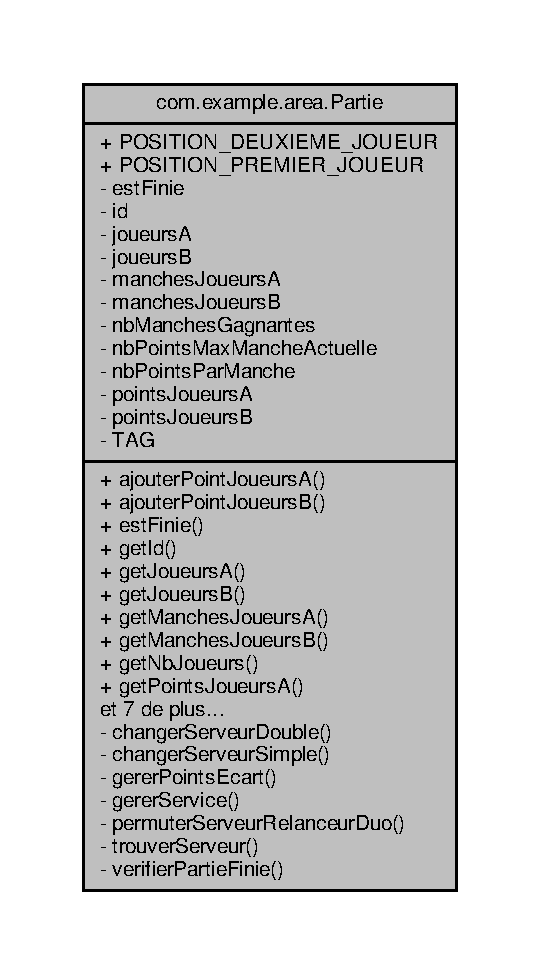
\includegraphics[width=259pt]{classcom_1_1example_1_1area_1_1_partie__coll__graph}
\end{center}
\end{figure}
\subsubsection*{Fonctions membres publiques}
\begin{DoxyCompactItemize}
\item 
void \hyperlink{classcom_1_1example_1_1area_1_1_partie_abb040a8be4a92a91afded80991d07087}{ajouter\+Point\+JoueursA} ()
\begin{DoxyCompactList}\small\item\em Méthode permettant d\textquotesingle{}incrémenter le score des joueursA. \end{DoxyCompactList}\item 
void \hyperlink{classcom_1_1example_1_1area_1_1_partie_aadc82cc11b982008b81f886adbc4e63a}{ajouter\+Point\+JoueursB} ()
\begin{DoxyCompactList}\small\item\em Méthode permettant d\textquotesingle{}incrémenter le score des joueursB. \end{DoxyCompactList}\item 
boolean \hyperlink{classcom_1_1example_1_1area_1_1_partie_ab0dd955a65440cab1569311ff35de3eb}{est\+Finie} ()
\begin{DoxyCompactList}\small\item\em Accesseur de l\textquotesingle{}attribut est\+Finie. \end{DoxyCompactList}\item 
int \hyperlink{classcom_1_1example_1_1area_1_1_partie_a535a67141814a238c1ffc0c42d0afedc}{get\+Id} ()
\begin{DoxyCompactList}\small\item\em Accesseur de l\textquotesingle{}attribut iD. \end{DoxyCompactList}\item 
Vector$<$ \hyperlink{classcom_1_1example_1_1area_1_1_joueur}{Joueur} $>$ \hyperlink{classcom_1_1example_1_1area_1_1_partie_a0f944de317206d9b99f9ffc7146a43ef}{get\+JoueursA} ()
\begin{DoxyCompactList}\small\item\em Accesseur de l\textquotesingle{}attribut joueursA. \end{DoxyCompactList}\item 
Vector$<$ \hyperlink{classcom_1_1example_1_1area_1_1_joueur}{Joueur} $>$ \hyperlink{classcom_1_1example_1_1area_1_1_partie_a3c6b981de54d03eeb553919983ee3be8}{get\+JoueursB} ()
\begin{DoxyCompactList}\small\item\em Accesseur de l\textquotesingle{}attribut joueursB. \end{DoxyCompactList}\item 
int \hyperlink{classcom_1_1example_1_1area_1_1_partie_a7c863edbbdd07ddc7f71616949823201}{get\+Manches\+JoueursA} ()
\begin{DoxyCompactList}\small\item\em Accesseur de l\textquotesingle{}attribut manches\+JoueursA. \end{DoxyCompactList}\item 
int \hyperlink{classcom_1_1example_1_1area_1_1_partie_a706fa101c4fcad9f2ea6473b5778b55e}{get\+Manches\+JoueursB} ()
\begin{DoxyCompactList}\small\item\em Accesseur de l\textquotesingle{}attribut manches\+JoueursB. \end{DoxyCompactList}\item 
int \hyperlink{classcom_1_1example_1_1area_1_1_partie_a70ddc06f598fa7ffb00c315fc9490647}{get\+Nb\+Joueurs} ()
\begin{DoxyCompactList}\small\item\em Retourne le nombre de joueurs dans la partie. \end{DoxyCompactList}\item 
int \hyperlink{classcom_1_1example_1_1area_1_1_partie_a5ec15306fc24648c1698ea0cdd50bf53}{get\+Points\+JoueursA} ()
\begin{DoxyCompactList}\small\item\em Accesseur de l\textquotesingle{}attribut points\+JoueursA. \end{DoxyCompactList}\item 
int \hyperlink{classcom_1_1example_1_1area_1_1_partie_a376bb79a67c311e1eb681387e9440bbd}{get\+Points\+JoueursB} ()
\begin{DoxyCompactList}\small\item\em Accesseur de l\textquotesingle{}attribut points\+JoueursB. \end{DoxyCompactList}\item 
\hyperlink{classcom_1_1example_1_1area_1_1_joueur}{Joueur} \hyperlink{classcom_1_1example_1_1area_1_1_partie_a34f75da57f51b710fccbce4aafda28d4}{get\+Serveur} ()
\begin{DoxyCompactList}\small\item\em Trouve le serveur et le retourne. \end{DoxyCompactList}\item 
\hyperlink{classcom_1_1example_1_1area_1_1_partie_a147e80f330c0236dbe800f5e2b4c2c84}{Partie} (int \hyperlink{classcom_1_1example_1_1area_1_1_partie_a1d1d6ce602fecf229217fe3d7a4d9152}{nb\+Manches\+Gagnantes}, int \hyperlink{classcom_1_1example_1_1area_1_1_partie_a23cd7e19042eece7057f810bba2f4f2c}{nb\+Points\+Par\+Manche}, Vector$<$ \hyperlink{classcom_1_1example_1_1area_1_1_joueur}{Joueur} $>$ \hyperlink{classcom_1_1example_1_1area_1_1_partie_a190a033a96ec435589ac53f78d60890b}{joueursA}, Vector$<$ \hyperlink{classcom_1_1example_1_1area_1_1_joueur}{Joueur} $>$ \hyperlink{classcom_1_1example_1_1area_1_1_partie_a208910b83df461c3a2503f3b28650ce8}{joueursB})
\item 
void \hyperlink{classcom_1_1example_1_1area_1_1_partie_a2847b07aff035a02c130f6219efc5312}{retirer\+Point\+JoueursA} ()
\begin{DoxyCompactList}\small\item\em Méthode permettant de décrémenter le score des joueursA. \end{DoxyCompactList}\item 
void \hyperlink{classcom_1_1example_1_1area_1_1_partie_aa3f7d2c68dcf31a2e48f95c5db9c5663}{retirer\+Point\+JoueursB} ()
\begin{DoxyCompactList}\small\item\em Méthode permettant de décrémenter le score des joueursB. \end{DoxyCompactList}\item 
void \hyperlink{classcom_1_1example_1_1area_1_1_partie_ace9c70bf0685d426f0d3fdb7e4f81f3f}{set\+JoueursA} (Vector$<$ \hyperlink{classcom_1_1example_1_1area_1_1_joueur}{Joueur} $>$ \hyperlink{classcom_1_1example_1_1area_1_1_partie_a190a033a96ec435589ac53f78d60890b}{joueursA})
\begin{DoxyCompactList}\small\item\em Mutateur de l\textquotesingle{}attribut joueursA. \end{DoxyCompactList}\item 
void \hyperlink{classcom_1_1example_1_1area_1_1_partie_a3f3cc9b2ddd055945b8b0835d0e7466b}{set\+JoueursB} (Vector$<$ \hyperlink{classcom_1_1example_1_1area_1_1_joueur}{Joueur} $>$ \hyperlink{classcom_1_1example_1_1area_1_1_partie_a208910b83df461c3a2503f3b28650ce8}{joueursB})
\begin{DoxyCompactList}\small\item\em Mutateur de l\textquotesingle{}attribut joueursB. \end{DoxyCompactList}\end{DoxyCompactItemize}
\subsubsection*{Attributs publics statiques}
\begin{DoxyCompactItemize}
\item 
static final int \hyperlink{classcom_1_1example_1_1area_1_1_partie_a6b5837dffa2af6a8da369f69916498f4}{P\+O\+S\+I\+T\+I\+O\+N\+\_\+\+D\+E\+U\+X\+I\+E\+M\+E\+\_\+\+J\+O\+U\+E\+UR} = 1
\item 
static final int \hyperlink{classcom_1_1example_1_1area_1_1_partie_a2f977d38424ff199a053d9e3cd4eb8c6}{P\+O\+S\+I\+T\+I\+O\+N\+\_\+\+P\+R\+E\+M\+I\+E\+R\+\_\+\+J\+O\+U\+E\+UR} = 0
\end{DoxyCompactItemize}
\subsubsection*{Fonctions membres privées}
\begin{DoxyCompactItemize}
\item 
void \hyperlink{classcom_1_1example_1_1area_1_1_partie_a14ae07774755900e3ae4e7e6808126c6}{changer\+Serveur\+Double} ()
\begin{DoxyCompactList}\small\item\em Méthode permettant de changer le serveur de duo en double. \end{DoxyCompactList}\item 
void \hyperlink{classcom_1_1example_1_1area_1_1_partie_ad6d7eef6348a783f9cdd0eb3dd14793d}{changer\+Serveur\+Simple} ()
\begin{DoxyCompactList}\small\item\em Méthode permettant de changer le serveur en simple. \end{DoxyCompactList}\item 
void \hyperlink{classcom_1_1example_1_1area_1_1_partie_a2838da99f206d736a22f8a3f271365b2}{gerer\+Points\+Ecart} ()
\begin{DoxyCompactList}\small\item\em Méthode permettant de gérer les points d\textquotesingle{}écarts lors d\textquotesingle{}une manche. \end{DoxyCompactList}\item 
void \hyperlink{classcom_1_1example_1_1area_1_1_partie_a52c8e133b23468d4b2c4338a80c3763c}{gerer\+Service} ()
\begin{DoxyCompactList}\small\item\em Méthode permettant de gérer l\textquotesingle{}attribution du service. \end{DoxyCompactList}\item 
Vector$<$ \hyperlink{classcom_1_1example_1_1area_1_1_joueur}{Joueur} $>$ \hyperlink{classcom_1_1example_1_1area_1_1_partie_a3143072ab9e3a306a42a84ecac4bdcf1}{permuter\+Serveur\+Relanceur\+Duo} (Vector$<$ \hyperlink{classcom_1_1example_1_1area_1_1_joueur}{Joueur} $>$ duo, \hyperlink{classcom_1_1example_1_1area_1_1_joueur}{Joueur} serveur)
\begin{DoxyCompactList}\small\item\em Méthode permettant de changer le serveur au sein d\textquotesingle{}un duo en double. \end{DoxyCompactList}\item 
\hyperlink{classcom_1_1example_1_1area_1_1_joueur}{Joueur} \hyperlink{classcom_1_1example_1_1area_1_1_partie_a34c737de89dee9e2510fa5959e238a3e}{trouver\+Serveur} (Vector$<$ \hyperlink{classcom_1_1example_1_1area_1_1_joueur}{Joueur} $>$ joueurs)
\begin{DoxyCompactList}\small\item\em Trouve le serveur dans un vecteur de joueurs puis retourne ce joueur ou null si il n\textquotesingle{}y en a aucun. \end{DoxyCompactList}\item 
void \hyperlink{classcom_1_1example_1_1area_1_1_partie_ad07c65c2ba36cd08798cee1ba6b99c81}{verifier\+Partie\+Finie} ()
\begin{DoxyCompactList}\small\item\em Méthode permettant de vérifier si la partie est finie. \end{DoxyCompactList}\end{DoxyCompactItemize}
\subsubsection*{Attributs privés}
\begin{DoxyCompactItemize}
\item 
boolean \hyperlink{classcom_1_1example_1_1area_1_1_partie_a00890390c78922c024fe31065923964e}{est\+Finie}
\item 
int \hyperlink{classcom_1_1example_1_1area_1_1_partie_a06ef6dd2585a669a8230ed1217cd98f4}{id}
\item 
Vector$<$ \hyperlink{classcom_1_1example_1_1area_1_1_joueur}{Joueur} $>$ \hyperlink{classcom_1_1example_1_1area_1_1_partie_a190a033a96ec435589ac53f78d60890b}{joueursA}
\item 
Vector$<$ \hyperlink{classcom_1_1example_1_1area_1_1_joueur}{Joueur} $>$ \hyperlink{classcom_1_1example_1_1area_1_1_partie_a208910b83df461c3a2503f3b28650ce8}{joueursB}
\item 
int \hyperlink{classcom_1_1example_1_1area_1_1_partie_a4563ef3464c670e68405bb7256abb770}{manches\+JoueursA}
\item 
int \hyperlink{classcom_1_1example_1_1area_1_1_partie_a9bb9a60be0b966b5a8bd5ac0934387bf}{manches\+JoueursB}
\item 
int \hyperlink{classcom_1_1example_1_1area_1_1_partie_a1d1d6ce602fecf229217fe3d7a4d9152}{nb\+Manches\+Gagnantes}
\item 
int \hyperlink{classcom_1_1example_1_1area_1_1_partie_a4b5e5464eb3b37f7c78d4134bf29a7f8}{nb\+Points\+Max\+Manche\+Actuelle}
\item 
int \hyperlink{classcom_1_1example_1_1area_1_1_partie_a23cd7e19042eece7057f810bba2f4f2c}{nb\+Points\+Par\+Manche}
\item 
int \hyperlink{classcom_1_1example_1_1area_1_1_partie_ad1075e561acb71ac3307570f79795b1c}{points\+JoueursA}
\item 
int \hyperlink{classcom_1_1example_1_1area_1_1_partie_ae1ceb321b45437487124b1d886c7297c}{points\+JoueursB}
\end{DoxyCompactItemize}
\subsubsection*{Attributs privés statiques}
\begin{DoxyCompactItemize}
\item 
static final String \hyperlink{classcom_1_1example_1_1area_1_1_partie_ac0444402f7c570474df1c8b7ece88ad9}{T\+AG} = \char`\"{}\+\_\+\+Partie\char`\"{}
\end{DoxyCompactItemize}


\subsubsection{Description détaillée}
Classe permettant la gestion d\textquotesingle{}une partie. 

Définition à la ligne \hyperlink{_partie_8java_source_l00022}{22} du fichier \hyperlink{_partie_8java_source}{Partie.\+java}.



\subsubsection{Documentation des constructeurs et destructeur}
\mbox{\Hypertarget{classcom_1_1example_1_1area_1_1_partie_a147e80f330c0236dbe800f5e2b4c2c84}\label{classcom_1_1example_1_1area_1_1_partie_a147e80f330c0236dbe800f5e2b4c2c84}} 
\index{com\+::example\+::area\+::\+Partie@{com\+::example\+::area\+::\+Partie}!Partie@{Partie}}
\index{Partie@{Partie}!com\+::example\+::area\+::\+Partie@{com\+::example\+::area\+::\+Partie}}
\paragraph{\texorpdfstring{Partie()}{Partie()}}
{\footnotesize\ttfamily com.\+example.\+area.\+Partie.\+Partie (\begin{DoxyParamCaption}\item[{int}]{nb\+Manches\+Gagnantes,  }\item[{int}]{nb\+Points\+Par\+Manche,  }\item[{Vector$<$ \hyperlink{classcom_1_1example_1_1area_1_1_joueur}{Joueur} $>$}]{joueursA,  }\item[{Vector$<$ \hyperlink{classcom_1_1example_1_1area_1_1_joueur}{Joueur} $>$}]{joueursB }\end{DoxyParamCaption})}



Définition à la ligne \hyperlink{_partie_8java_source_l00046}{46} du fichier \hyperlink{_partie_8java_source}{Partie.\+java}.



Références \hyperlink{_partie_8java_source_l00037}{com.\+example.\+area.\+Partie.\+joueursA}, \hyperlink{_partie_8java_source_l00038}{com.\+example.\+area.\+Partie.\+joueursB}, \hyperlink{_partie_8java_source_l00034}{com.\+example.\+area.\+Partie.\+nb\+Manches\+Gagnantes}, et \hyperlink{_partie_8java_source_l00035}{com.\+example.\+area.\+Partie.\+nb\+Points\+Par\+Manche}.


\begin{DoxyCode}
00047     \{
00048         this.\hyperlink{classcom_1_1example_1_1area_1_1_partie_a1d1d6ce602fecf229217fe3d7a4d9152}{nbManchesGagnantes} = \hyperlink{classcom_1_1example_1_1area_1_1_partie_a1d1d6ce602fecf229217fe3d7a4d9152}{nbManchesGagnantes};
00049         this.\hyperlink{classcom_1_1example_1_1area_1_1_partie_a23cd7e19042eece7057f810bba2f4f2c}{nbPointsParManche} = \hyperlink{classcom_1_1example_1_1area_1_1_partie_a23cd7e19042eece7057f810bba2f4f2c}{nbPointsParManche};
00050         this.\hyperlink{classcom_1_1example_1_1area_1_1_partie_a4b5e5464eb3b37f7c78d4134bf29a7f8}{nbPointsMaxMancheActuelle} = 
      \hyperlink{classcom_1_1example_1_1area_1_1_partie_a23cd7e19042eece7057f810bba2f4f2c}{nbPointsParManche};
00051         this.\hyperlink{classcom_1_1example_1_1area_1_1_partie_ab0dd955a65440cab1569311ff35de3eb}{estFinie} = \textcolor{keyword}{false};
00052         this.\hyperlink{classcom_1_1example_1_1area_1_1_partie_ad1075e561acb71ac3307570f79795b1c}{pointsJoueursA} = 0;
00053         this.\hyperlink{classcom_1_1example_1_1area_1_1_partie_ae1ceb321b45437487124b1d886c7297c}{pointsJoueursB} = 0;
00054         this.\hyperlink{classcom_1_1example_1_1area_1_1_partie_a4563ef3464c670e68405bb7256abb770}{manchesJoueursA} = 0;
00055         this.\hyperlink{classcom_1_1example_1_1area_1_1_partie_a9bb9a60be0b966b5a8bd5ac0934387bf}{manchesJoueursB} = 0;
00056         this.\textcolor{keywordtype}{id} = 0;
00057         this.\hyperlink{classcom_1_1example_1_1area_1_1_partie_a190a033a96ec435589ac53f78d60890b}{joueursA} = \hyperlink{classcom_1_1example_1_1area_1_1_partie_a190a033a96ec435589ac53f78d60890b}{joueursA};
00058         this.\hyperlink{classcom_1_1example_1_1area_1_1_partie_a208910b83df461c3a2503f3b28650ce8}{joueursB} = \hyperlink{classcom_1_1example_1_1area_1_1_partie_a208910b83df461c3a2503f3b28650ce8}{joueursB};
00059     \}
\end{DoxyCode}


\subsubsection{Documentation des fonctions membres}
\mbox{\Hypertarget{classcom_1_1example_1_1area_1_1_partie_abb040a8be4a92a91afded80991d07087}\label{classcom_1_1example_1_1area_1_1_partie_abb040a8be4a92a91afded80991d07087}} 
\index{com\+::example\+::area\+::\+Partie@{com\+::example\+::area\+::\+Partie}!ajouter\+Point\+JoueursA@{ajouter\+Point\+JoueursA}}
\index{ajouter\+Point\+JoueursA@{ajouter\+Point\+JoueursA}!com\+::example\+::area\+::\+Partie@{com\+::example\+::area\+::\+Partie}}
\paragraph{\texorpdfstring{ajouter\+Point\+Joueurs\+A()}{ajouterPointJoueursA()}}
{\footnotesize\ttfamily void com.\+example.\+area.\+Partie.\+ajouter\+Point\+JoueursA (\begin{DoxyParamCaption}{ }\end{DoxyParamCaption})}



Méthode permettant d\textquotesingle{}incrémenter le score des joueursA. 



Définition à la ligne \hyperlink{_partie_8java_source_l00128}{128} du fichier \hyperlink{_partie_8java_source}{Partie.\+java}.



Références \hyperlink{_partie_8java_source_l00204}{com.\+example.\+area.\+Partie.\+gerer\+Points\+Ecart()}, \hyperlink{_partie_8java_source_l00220}{com.\+example.\+area.\+Partie.\+gerer\+Service()}, \hyperlink{_partie_8java_source_l00035}{com.\+example.\+area.\+Partie.\+nb\+Points\+Par\+Manche}, et \hyperlink{_partie_8java_source_l00192}{com.\+example.\+area.\+Partie.\+verifier\+Partie\+Finie()}.



Référencé par \hyperlink{_i_h_m_gestion_partie_8java_source_l00346}{com.\+example.\+area.\+I\+H\+M\+Gestion\+Partie.\+connecter\+Boutons()}.


\begin{DoxyCode}
00129     \{
00130         \hyperlink{classcom_1_1example_1_1area_1_1_partie_ad1075e561acb71ac3307570f79795b1c}{pointsJoueursA}++;
00131         \hyperlink{classcom_1_1example_1_1area_1_1_partie_a2838da99f206d736a22f8a3f271365b2}{gererPointsEcart}();
00132         \hyperlink{classcom_1_1example_1_1area_1_1_partie_a52c8e133b23468d4b2c4338a80c3763c}{gererService}();
00133 
00134         \textcolor{keywordflow}{if} (\hyperlink{classcom_1_1example_1_1area_1_1_partie_ad1075e561acb71ac3307570f79795b1c}{pointsJoueursA} == \hyperlink{classcom_1_1example_1_1area_1_1_partie_a4b5e5464eb3b37f7c78d4134bf29a7f8}{nbPointsMaxMancheActuelle})
00135         \{
00136             \hyperlink{classcom_1_1example_1_1area_1_1_partie_a4563ef3464c670e68405bb7256abb770}{manchesJoueursA}++;
00137             \hyperlink{classcom_1_1example_1_1area_1_1_partie_ad1075e561acb71ac3307570f79795b1c}{pointsJoueursA} = 0;
00138             \hyperlink{classcom_1_1example_1_1area_1_1_partie_ae1ceb321b45437487124b1d886c7297c}{pointsJoueursB} = 0;
00139             \hyperlink{classcom_1_1example_1_1area_1_1_partie_a4b5e5464eb3b37f7c78d4134bf29a7f8}{nbPointsMaxMancheActuelle} = 
      \hyperlink{classcom_1_1example_1_1area_1_1_partie_a23cd7e19042eece7057f810bba2f4f2c}{nbPointsParManche};
00140             \hyperlink{classcom_1_1example_1_1area_1_1_partie_ad07c65c2ba36cd08798cee1ba6b99c81}{verifierPartieFinie}();
00141         \}
00142     \}
\end{DoxyCode}
\mbox{\Hypertarget{classcom_1_1example_1_1area_1_1_partie_aadc82cc11b982008b81f886adbc4e63a}\label{classcom_1_1example_1_1area_1_1_partie_aadc82cc11b982008b81f886adbc4e63a}} 
\index{com\+::example\+::area\+::\+Partie@{com\+::example\+::area\+::\+Partie}!ajouter\+Point\+JoueursB@{ajouter\+Point\+JoueursB}}
\index{ajouter\+Point\+JoueursB@{ajouter\+Point\+JoueursB}!com\+::example\+::area\+::\+Partie@{com\+::example\+::area\+::\+Partie}}
\paragraph{\texorpdfstring{ajouter\+Point\+Joueurs\+B()}{ajouterPointJoueursB()}}
{\footnotesize\ttfamily void com.\+example.\+area.\+Partie.\+ajouter\+Point\+JoueursB (\begin{DoxyParamCaption}{ }\end{DoxyParamCaption})}



Méthode permettant d\textquotesingle{}incrémenter le score des joueursB. 



Définition à la ligne \hyperlink{_partie_8java_source_l00147}{147} du fichier \hyperlink{_partie_8java_source}{Partie.\+java}.



Références \hyperlink{_partie_8java_source_l00204}{com.\+example.\+area.\+Partie.\+gerer\+Points\+Ecart()}, \hyperlink{_partie_8java_source_l00220}{com.\+example.\+area.\+Partie.\+gerer\+Service()}, \hyperlink{_partie_8java_source_l00035}{com.\+example.\+area.\+Partie.\+nb\+Points\+Par\+Manche}, et \hyperlink{_partie_8java_source_l00192}{com.\+example.\+area.\+Partie.\+verifier\+Partie\+Finie()}.



Référencé par \hyperlink{_i_h_m_gestion_partie_8java_source_l00346}{com.\+example.\+area.\+I\+H\+M\+Gestion\+Partie.\+connecter\+Boutons()}.


\begin{DoxyCode}
00148     \{
00149         \hyperlink{classcom_1_1example_1_1area_1_1_partie_ae1ceb321b45437487124b1d886c7297c}{pointsJoueursB}++;
00150         \hyperlink{classcom_1_1example_1_1area_1_1_partie_a2838da99f206d736a22f8a3f271365b2}{gererPointsEcart}();
00151         \hyperlink{classcom_1_1example_1_1area_1_1_partie_a52c8e133b23468d4b2c4338a80c3763c}{gererService}();
00152 
00153         \textcolor{keywordflow}{if} (\hyperlink{classcom_1_1example_1_1area_1_1_partie_ae1ceb321b45437487124b1d886c7297c}{pointsJoueursB} == \hyperlink{classcom_1_1example_1_1area_1_1_partie_a4b5e5464eb3b37f7c78d4134bf29a7f8}{nbPointsMaxMancheActuelle})
00154         \{
00155             \hyperlink{classcom_1_1example_1_1area_1_1_partie_a9bb9a60be0b966b5a8bd5ac0934387bf}{manchesJoueursB}++;
00156             \hyperlink{classcom_1_1example_1_1area_1_1_partie_ad1075e561acb71ac3307570f79795b1c}{pointsJoueursA} = 0;
00157             \hyperlink{classcom_1_1example_1_1area_1_1_partie_ae1ceb321b45437487124b1d886c7297c}{pointsJoueursB} = 0;
00158             \hyperlink{classcom_1_1example_1_1area_1_1_partie_a4b5e5464eb3b37f7c78d4134bf29a7f8}{nbPointsMaxMancheActuelle} = 
      \hyperlink{classcom_1_1example_1_1area_1_1_partie_a23cd7e19042eece7057f810bba2f4f2c}{nbPointsParManche};
00159             \hyperlink{classcom_1_1example_1_1area_1_1_partie_ad07c65c2ba36cd08798cee1ba6b99c81}{verifierPartieFinie}();
00160         \}
00161     \}
\end{DoxyCode}
\mbox{\Hypertarget{classcom_1_1example_1_1area_1_1_partie_a14ae07774755900e3ae4e7e6808126c6}\label{classcom_1_1example_1_1area_1_1_partie_a14ae07774755900e3ae4e7e6808126c6}} 
\index{com\+::example\+::area\+::\+Partie@{com\+::example\+::area\+::\+Partie}!changer\+Serveur\+Double@{changer\+Serveur\+Double}}
\index{changer\+Serveur\+Double@{changer\+Serveur\+Double}!com\+::example\+::area\+::\+Partie@{com\+::example\+::area\+::\+Partie}}
\paragraph{\texorpdfstring{changer\+Serveur\+Double()}{changerServeurDouble()}}
{\footnotesize\ttfamily void com.\+example.\+area.\+Partie.\+changer\+Serveur\+Double (\begin{DoxyParamCaption}{ }\end{DoxyParamCaption})\hspace{0.3cm}{\ttfamily [private]}}



Méthode permettant de changer le serveur de duo en double. 



Définition à la ligne \hyperlink{_partie_8java_source_l00253}{253} du fichier \hyperlink{_partie_8java_source}{Partie.\+java}.



Références \hyperlink{_partie_8java_source_l00315}{com.\+example.\+area.\+Partie.\+trouver\+Serveur()}.



Référencé par \hyperlink{_partie_8java_source_l00220}{com.\+example.\+area.\+Partie.\+gerer\+Service()}.


\begin{DoxyCode}
00254     \{
00255         Joueur serveur = null;
00256         serveur = \hyperlink{classcom_1_1example_1_1area_1_1_partie_a34c737de89dee9e2510fa5959e238a3e}{trouverServeur}(\hyperlink{classcom_1_1example_1_1area_1_1_partie_a190a033a96ec435589ac53f78d60890b}{joueursA});
00257         \textcolor{keywordtype}{int} indexServeur = 0;
00258         \textcolor{keywordflow}{if} (serveur != null)
00259         \{
00260             indexServeur = \hyperlink{classcom_1_1example_1_1area_1_1_partie_a190a033a96ec435589ac53f78d60890b}{joueursA}.indexOf(serveur);
00261             \hyperlink{classcom_1_1example_1_1area_1_1_partie_a208910b83df461c3a2503f3b28650ce8}{joueursB}.elementAt(indexServeur).setEstServeur(\textcolor{keyword}{true});
00262             \hyperlink{classcom_1_1example_1_1area_1_1_partie_a190a033a96ec435589ac53f78d60890b}{joueursA}.elementAt(indexServeur).setEstServeur(\textcolor{keyword}{false});
00263         \}
00264         \textcolor{keywordflow}{else}
00265         \{
00266             serveur = \hyperlink{classcom_1_1example_1_1area_1_1_partie_a34c737de89dee9e2510fa5959e238a3e}{trouverServeur}(\hyperlink{classcom_1_1example_1_1area_1_1_partie_a208910b83df461c3a2503f3b28650ce8}{joueursB});
00267             indexServeur = \hyperlink{classcom_1_1example_1_1area_1_1_partie_a208910b83df461c3a2503f3b28650ce8}{joueursB}.indexOf(serveur);
00268             \hyperlink{classcom_1_1example_1_1area_1_1_partie_a190a033a96ec435589ac53f78d60890b}{joueursA}.elementAt(indexServeur).setEstServeur(\textcolor{keyword}{true});
00269             \hyperlink{classcom_1_1example_1_1area_1_1_partie_a208910b83df461c3a2503f3b28650ce8}{joueursB}.elementAt(indexServeur).setEstServeur(\textcolor{keyword}{false});
00270         \}
00271     \}
\end{DoxyCode}
\mbox{\Hypertarget{classcom_1_1example_1_1area_1_1_partie_ad6d7eef6348a783f9cdd0eb3dd14793d}\label{classcom_1_1example_1_1area_1_1_partie_ad6d7eef6348a783f9cdd0eb3dd14793d}} 
\index{com\+::example\+::area\+::\+Partie@{com\+::example\+::area\+::\+Partie}!changer\+Serveur\+Simple@{changer\+Serveur\+Simple}}
\index{changer\+Serveur\+Simple@{changer\+Serveur\+Simple}!com\+::example\+::area\+::\+Partie@{com\+::example\+::area\+::\+Partie}}
\paragraph{\texorpdfstring{changer\+Serveur\+Simple()}{changerServeurSimple()}}
{\footnotesize\ttfamily void com.\+example.\+area.\+Partie.\+changer\+Serveur\+Simple (\begin{DoxyParamCaption}{ }\end{DoxyParamCaption})\hspace{0.3cm}{\ttfamily [private]}}



Méthode permettant de changer le serveur en simple. 



Définition à la ligne \hyperlink{_partie_8java_source_l00276}{276} du fichier \hyperlink{_partie_8java_source}{Partie.\+java}.



Référencé par \hyperlink{_partie_8java_source_l00220}{com.\+example.\+area.\+Partie.\+gerer\+Service()}.


\begin{DoxyCode}
00277     \{
00278         \textcolor{keywordflow}{if} (\hyperlink{classcom_1_1example_1_1area_1_1_partie_a190a033a96ec435589ac53f78d60890b}{joueursA}.elementAt(\hyperlink{classcom_1_1example_1_1area_1_1_partie_a2f977d38424ff199a053d9e3cd4eb8c6}{POSITION\_PREMIER\_JOUEUR}).estServeur())
00279         \{
00280             \hyperlink{classcom_1_1example_1_1area_1_1_partie_a190a033a96ec435589ac53f78d60890b}{joueursA}.elementAt(\hyperlink{classcom_1_1example_1_1area_1_1_partie_a2f977d38424ff199a053d9e3cd4eb8c6}{POSITION\_PREMIER\_JOUEUR}).setEstServeur(\textcolor{keyword}{false})
      ;
00281             \hyperlink{classcom_1_1example_1_1area_1_1_partie_a208910b83df461c3a2503f3b28650ce8}{joueursB}.elementAt(\hyperlink{classcom_1_1example_1_1area_1_1_partie_a2f977d38424ff199a053d9e3cd4eb8c6}{POSITION\_PREMIER\_JOUEUR}).setEstServeur(\textcolor{keyword}{true});
00282         \}
00283         \textcolor{keywordflow}{else}
00284         \{
00285             \hyperlink{classcom_1_1example_1_1area_1_1_partie_a208910b83df461c3a2503f3b28650ce8}{joueursB}.elementAt(\hyperlink{classcom_1_1example_1_1area_1_1_partie_a2f977d38424ff199a053d9e3cd4eb8c6}{POSITION\_PREMIER\_JOUEUR}).setEstServeur(\textcolor{keyword}{false})
      ;
00286             \hyperlink{classcom_1_1example_1_1area_1_1_partie_a190a033a96ec435589ac53f78d60890b}{joueursA}.elementAt(\hyperlink{classcom_1_1example_1_1area_1_1_partie_a2f977d38424ff199a053d9e3cd4eb8c6}{POSITION\_PREMIER\_JOUEUR}).setEstServeur(\textcolor{keyword}{true});
00287         \}
00288     \}
\end{DoxyCode}
\mbox{\Hypertarget{classcom_1_1example_1_1area_1_1_partie_ab0dd955a65440cab1569311ff35de3eb}\label{classcom_1_1example_1_1area_1_1_partie_ab0dd955a65440cab1569311ff35de3eb}} 
\index{com\+::example\+::area\+::\+Partie@{com\+::example\+::area\+::\+Partie}!est\+Finie@{est\+Finie}}
\index{est\+Finie@{est\+Finie}!com\+::example\+::area\+::\+Partie@{com\+::example\+::area\+::\+Partie}}
\paragraph{\texorpdfstring{est\+Finie()}{estFinie()}}
{\footnotesize\ttfamily boolean com.\+example.\+area.\+Partie.\+est\+Finie (\begin{DoxyParamCaption}{ }\end{DoxyParamCaption})}



Accesseur de l\textquotesingle{}attribut est\+Finie. 



Définition à la ligne \hyperlink{_partie_8java_source_l00120}{120} du fichier \hyperlink{_partie_8java_source}{Partie.\+java}.


\begin{DoxyCode}
00121     \{
00122         \textcolor{keywordflow}{return} \hyperlink{classcom_1_1example_1_1area_1_1_partie_ab0dd955a65440cab1569311ff35de3eb}{estFinie};
00123     \}
\end{DoxyCode}
\mbox{\Hypertarget{classcom_1_1example_1_1area_1_1_partie_a2838da99f206d736a22f8a3f271365b2}\label{classcom_1_1example_1_1area_1_1_partie_a2838da99f206d736a22f8a3f271365b2}} 
\index{com\+::example\+::area\+::\+Partie@{com\+::example\+::area\+::\+Partie}!gerer\+Points\+Ecart@{gerer\+Points\+Ecart}}
\index{gerer\+Points\+Ecart@{gerer\+Points\+Ecart}!com\+::example\+::area\+::\+Partie@{com\+::example\+::area\+::\+Partie}}
\paragraph{\texorpdfstring{gerer\+Points\+Ecart()}{gererPointsEcart()}}
{\footnotesize\ttfamily void com.\+example.\+area.\+Partie.\+gerer\+Points\+Ecart (\begin{DoxyParamCaption}{ }\end{DoxyParamCaption})\hspace{0.3cm}{\ttfamily [private]}}



Méthode permettant de gérer les points d\textquotesingle{}écarts lors d\textquotesingle{}une manche. 



Définition à la ligne \hyperlink{_partie_8java_source_l00204}{204} du fichier \hyperlink{_partie_8java_source}{Partie.\+java}.



Référencé par \hyperlink{_partie_8java_source_l00128}{com.\+example.\+area.\+Partie.\+ajouter\+Point\+Joueurs\+A()}, \hyperlink{_partie_8java_source_l00147}{com.\+example.\+area.\+Partie.\+ajouter\+Point\+Joueurs\+B()}, \hyperlink{_partie_8java_source_l00166}{com.\+example.\+area.\+Partie.\+retirer\+Point\+Joueurs\+A()}, et \hyperlink{_partie_8java_source_l00179}{com.\+example.\+area.\+Partie.\+retirer\+Point\+Joueurs\+B()}.


\begin{DoxyCode}
00205     \{
00206         \textcolor{keywordflow}{if} (\hyperlink{classcom_1_1example_1_1area_1_1_partie_ad1075e561acb71ac3307570f79795b1c}{pointsJoueursA} == \hyperlink{classcom_1_1example_1_1area_1_1_partie_ae1ceb321b45437487124b1d886c7297c}{pointsJoueursB} && (
      \hyperlink{classcom_1_1example_1_1area_1_1_partie_ad1075e561acb71ac3307570f79795b1c}{pointsJoueursA} == (\hyperlink{classcom_1_1example_1_1area_1_1_partie_a4b5e5464eb3b37f7c78d4134bf29a7f8}{nbPointsMaxMancheActuelle}-1 )))
00207         \{
00208             \hyperlink{classcom_1_1example_1_1area_1_1_partie_a4b5e5464eb3b37f7c78d4134bf29a7f8}{nbPointsMaxMancheActuelle}++;
00209         \}
00210         \textcolor{keywordflow}{else} \textcolor{keywordflow}{if} ( \hyperlink{classcom_1_1example_1_1area_1_1_partie_a4b5e5464eb3b37f7c78d4134bf29a7f8}{nbPointsMaxMancheActuelle} > 
      \hyperlink{classcom_1_1example_1_1area_1_1_partie_a23cd7e19042eece7057f810bba2f4f2c}{nbPointsParManche} && \hyperlink{classcom_1_1example_1_1area_1_1_partie_ad1075e561acb71ac3307570f79795b1c}{pointsJoueursA} == 
      \hyperlink{classcom_1_1example_1_1area_1_1_partie_ae1ceb321b45437487124b1d886c7297c}{pointsJoueursB} && (\hyperlink{classcom_1_1example_1_1area_1_1_partie_ad1075e561acb71ac3307570f79795b1c}{pointsJoueursA} == (
      \hyperlink{classcom_1_1example_1_1area_1_1_partie_a4b5e5464eb3b37f7c78d4134bf29a7f8}{nbPointsMaxMancheActuelle}-2 )))
00211         \{
00212             \hyperlink{classcom_1_1example_1_1area_1_1_partie_a4b5e5464eb3b37f7c78d4134bf29a7f8}{nbPointsMaxMancheActuelle}--;
00213         \}
00214         Log.d(\hyperlink{classcom_1_1example_1_1area_1_1_partie_ac0444402f7c570474df1c8b7ece88ad9}{TAG},\textcolor{stringliteral}{"nbPointsMaxMancheActuelle : "} + Integer.toString(
      \hyperlink{classcom_1_1example_1_1area_1_1_partie_a4b5e5464eb3b37f7c78d4134bf29a7f8}{nbPointsMaxMancheActuelle}));
00215     \}
\end{DoxyCode}
\mbox{\Hypertarget{classcom_1_1example_1_1area_1_1_partie_a52c8e133b23468d4b2c4338a80c3763c}\label{classcom_1_1example_1_1area_1_1_partie_a52c8e133b23468d4b2c4338a80c3763c}} 
\index{com\+::example\+::area\+::\+Partie@{com\+::example\+::area\+::\+Partie}!gerer\+Service@{gerer\+Service}}
\index{gerer\+Service@{gerer\+Service}!com\+::example\+::area\+::\+Partie@{com\+::example\+::area\+::\+Partie}}
\paragraph{\texorpdfstring{gerer\+Service()}{gererService()}}
{\footnotesize\ttfamily void com.\+example.\+area.\+Partie.\+gerer\+Service (\begin{DoxyParamCaption}{ }\end{DoxyParamCaption})\hspace{0.3cm}{\ttfamily [private]}}



Méthode permettant de gérer l\textquotesingle{}attribution du service. 



Définition à la ligne \hyperlink{_partie_8java_source_l00220}{220} du fichier \hyperlink{_partie_8java_source}{Partie.\+java}.



Références \hyperlink{_partie_8java_source_l00253}{com.\+example.\+area.\+Partie.\+changer\+Serveur\+Double()}, \hyperlink{_partie_8java_source_l00276}{com.\+example.\+area.\+Partie.\+changer\+Serveur\+Simple()}, \hyperlink{_partie_8java_source_l00293}{com.\+example.\+area.\+Partie.\+permuter\+Serveur\+Relanceur\+Duo()}, \hyperlink{_partie_8java_source_l00040}{com.\+example.\+area.\+Partie.\+points\+JoueursB}, et \hyperlink{_partie_8java_source_l00315}{com.\+example.\+area.\+Partie.\+trouver\+Serveur()}.



Référencé par \hyperlink{_partie_8java_source_l00128}{com.\+example.\+area.\+Partie.\+ajouter\+Point\+Joueurs\+A()}, \hyperlink{_partie_8java_source_l00147}{com.\+example.\+area.\+Partie.\+ajouter\+Point\+Joueurs\+B()}, \hyperlink{_partie_8java_source_l00166}{com.\+example.\+area.\+Partie.\+retirer\+Point\+Joueurs\+A()}, et \hyperlink{_partie_8java_source_l00179}{com.\+example.\+area.\+Partie.\+retirer\+Point\+Joueurs\+B()}.


\begin{DoxyCode}
00221     \{
00222         \textcolor{keywordtype}{int} pointsMarques = \hyperlink{classcom_1_1example_1_1area_1_1_partie_ad1075e561acb71ac3307570f79795b1c}{pointsJoueursA} + \hyperlink{classcom_1_1example_1_1area_1_1_partie_ae1ceb321b45437487124b1d886c7297c}{pointsJoueursB};
00223         \textcolor{keywordflow}{if}(pointsMarques % 2 == 0 && pointsMarques != 0)
00224         \{
00225             \textcolor{keywordflow}{if}(\hyperlink{classcom_1_1example_1_1area_1_1_partie_a190a033a96ec435589ac53f78d60890b}{joueursA}.size() == 1)
00226             \{
00227                 \hyperlink{classcom_1_1example_1_1area_1_1_partie_ad6d7eef6348a783f9cdd0eb3dd14793d}{changerServeurSimple}();
00228             \}
00229             \textcolor{keywordflow}{else}
00230             \{
00231                 \hyperlink{classcom_1_1example_1_1area_1_1_partie_a14ae07774755900e3ae4e7e6808126c6}{changerServeurDouble}();
00232             \}
00233         \}
00234         \textcolor{keywordflow}{else} \textcolor{keywordflow}{if} (\hyperlink{classcom_1_1example_1_1area_1_1_partie_a190a033a96ec435589ac53f78d60890b}{joueursA}.size() == 2)
00235         \{
00236             Joueur serveur = null;
00237             serveur = \hyperlink{classcom_1_1example_1_1area_1_1_partie_a34c737de89dee9e2510fa5959e238a3e}{trouverServeur}(\hyperlink{classcom_1_1example_1_1area_1_1_partie_a190a033a96ec435589ac53f78d60890b}{joueursA});
00238             \textcolor{keywordflow}{if} (serveur != null)
00239             \{
00240                 \hyperlink{classcom_1_1example_1_1area_1_1_partie_a190a033a96ec435589ac53f78d60890b}{joueursA} = \hyperlink{classcom_1_1example_1_1area_1_1_partie_a3143072ab9e3a306a42a84ecac4bdcf1}{permuterServeurRelanceurDuo}(
      \hyperlink{classcom_1_1example_1_1area_1_1_partie_a190a033a96ec435589ac53f78d60890b}{joueursA},serveur);
00241             \}
00242             \textcolor{keywordflow}{else}
00243             \{
00244                 serveur = \hyperlink{classcom_1_1example_1_1area_1_1_partie_a34c737de89dee9e2510fa5959e238a3e}{trouverServeur}(\hyperlink{classcom_1_1example_1_1area_1_1_partie_a208910b83df461c3a2503f3b28650ce8}{joueursB});
00245                 \hyperlink{classcom_1_1example_1_1area_1_1_partie_a208910b83df461c3a2503f3b28650ce8}{joueursB} = \hyperlink{classcom_1_1example_1_1area_1_1_partie_a3143072ab9e3a306a42a84ecac4bdcf1}{permuterServeurRelanceurDuo}(
      \hyperlink{classcom_1_1example_1_1area_1_1_partie_a208910b83df461c3a2503f3b28650ce8}{joueursB},serveur);
00246             \}
00247         \}
00248     \}
\end{DoxyCode}
\mbox{\Hypertarget{classcom_1_1example_1_1area_1_1_partie_a535a67141814a238c1ffc0c42d0afedc}\label{classcom_1_1example_1_1area_1_1_partie_a535a67141814a238c1ffc0c42d0afedc}} 
\index{com\+::example\+::area\+::\+Partie@{com\+::example\+::area\+::\+Partie}!get\+Id@{get\+Id}}
\index{get\+Id@{get\+Id}!com\+::example\+::area\+::\+Partie@{com\+::example\+::area\+::\+Partie}}
\paragraph{\texorpdfstring{get\+Id()}{getId()}}
{\footnotesize\ttfamily int com.\+example.\+area.\+Partie.\+get\+Id (\begin{DoxyParamCaption}{ }\end{DoxyParamCaption})}



Accesseur de l\textquotesingle{}attribut iD. 



Définition à la ligne \hyperlink{_partie_8java_source_l00112}{112} du fichier \hyperlink{_partie_8java_source}{Partie.\+java}.



Références \hyperlink{_partie_8java_source_l00043}{com.\+example.\+area.\+Partie.\+id}.



Référencé par \hyperlink{_protocol_a_r_e_a_8java_source_l00048}{com.\+example.\+area.\+Protocol\+A\+R\+E\+A.\+fabriquer\+Trame\+Afficheur()}.


\begin{DoxyCode}
00113     \{
00114         \textcolor{keywordflow}{return} \hyperlink{classcom_1_1example_1_1area_1_1_partie_a06ef6dd2585a669a8230ed1217cd98f4}{id};
00115     \}
\end{DoxyCode}
\mbox{\Hypertarget{classcom_1_1example_1_1area_1_1_partie_a0f944de317206d9b99f9ffc7146a43ef}\label{classcom_1_1example_1_1area_1_1_partie_a0f944de317206d9b99f9ffc7146a43ef}} 
\index{com\+::example\+::area\+::\+Partie@{com\+::example\+::area\+::\+Partie}!get\+JoueursA@{get\+JoueursA}}
\index{get\+JoueursA@{get\+JoueursA}!com\+::example\+::area\+::\+Partie@{com\+::example\+::area\+::\+Partie}}
\paragraph{\texorpdfstring{get\+Joueurs\+A()}{getJoueursA()}}
{\footnotesize\ttfamily Vector$<$\hyperlink{classcom_1_1example_1_1area_1_1_joueur}{Joueur}$>$ com.\+example.\+area.\+Partie.\+get\+JoueursA (\begin{DoxyParamCaption}{ }\end{DoxyParamCaption})}



Accesseur de l\textquotesingle{}attribut joueursA. 



Définition à la ligne \hyperlink{_partie_8java_source_l00064}{64} du fichier \hyperlink{_partie_8java_source}{Partie.\+java}.



Références \hyperlink{_partie_8java_source_l00037}{com.\+example.\+area.\+Partie.\+joueursA}.



Référencé par \hyperlink{_i_h_m_gestion_partie_8java_source_l00401}{com.\+example.\+area.\+I\+H\+M\+Gestion\+Partie.\+afficher\+Noms\+Joueurs\+A()}, \hyperlink{_i_h_m_gestion_partie_8java_source_l00447}{com.\+example.\+area.\+I\+H\+M\+Gestion\+Partie.\+afficher\+Serveur()}, \hyperlink{_i_h_m_gestion_rencontre_8java_source_l00222}{com.\+example.\+area.\+I\+H\+M\+Gestion\+Rencontre.\+demander\+Serveur()}, \hyperlink{_protocol_a_r_e_a_8java_source_l00048}{com.\+example.\+area.\+Protocol\+A\+R\+E\+A.\+fabriquer\+Trame\+Afficheur()}, et \hyperlink{_i_h_m_gestion_rencontre_8java_source_l00343}{com.\+example.\+area.\+I\+H\+M\+Gestion\+Rencontre.\+formater\+Partie()}.


\begin{DoxyCode}
00065     \{
00066         \textcolor{keywordflow}{return} \hyperlink{classcom_1_1example_1_1area_1_1_partie_a190a033a96ec435589ac53f78d60890b}{joueursA};
00067     \}
\end{DoxyCode}
\mbox{\Hypertarget{classcom_1_1example_1_1area_1_1_partie_a3c6b981de54d03eeb553919983ee3be8}\label{classcom_1_1example_1_1area_1_1_partie_a3c6b981de54d03eeb553919983ee3be8}} 
\index{com\+::example\+::area\+::\+Partie@{com\+::example\+::area\+::\+Partie}!get\+JoueursB@{get\+JoueursB}}
\index{get\+JoueursB@{get\+JoueursB}!com\+::example\+::area\+::\+Partie@{com\+::example\+::area\+::\+Partie}}
\paragraph{\texorpdfstring{get\+Joueurs\+B()}{getJoueursB()}}
{\footnotesize\ttfamily Vector$<$\hyperlink{classcom_1_1example_1_1area_1_1_joueur}{Joueur}$>$ com.\+example.\+area.\+Partie.\+get\+JoueursB (\begin{DoxyParamCaption}{ }\end{DoxyParamCaption})}



Accesseur de l\textquotesingle{}attribut joueursB. 



Définition à la ligne \hyperlink{_partie_8java_source_l00072}{72} du fichier \hyperlink{_partie_8java_source}{Partie.\+java}.



Références \hyperlink{_partie_8java_source_l00038}{com.\+example.\+area.\+Partie.\+joueursB}.



Référencé par \hyperlink{_i_h_m_gestion_partie_8java_source_l00418}{com.\+example.\+area.\+I\+H\+M\+Gestion\+Partie.\+afficher\+Noms\+Joueurs\+B()}, \hyperlink{_i_h_m_gestion_rencontre_8java_source_l00222}{com.\+example.\+area.\+I\+H\+M\+Gestion\+Rencontre.\+demander\+Serveur()}, et \hyperlink{_i_h_m_gestion_rencontre_8java_source_l00343}{com.\+example.\+area.\+I\+H\+M\+Gestion\+Rencontre.\+formater\+Partie()}.


\begin{DoxyCode}
00073     \{
00074         \textcolor{keywordflow}{return} \hyperlink{classcom_1_1example_1_1area_1_1_partie_a208910b83df461c3a2503f3b28650ce8}{joueursB};
00075     \}
\end{DoxyCode}
\mbox{\Hypertarget{classcom_1_1example_1_1area_1_1_partie_a7c863edbbdd07ddc7f71616949823201}\label{classcom_1_1example_1_1area_1_1_partie_a7c863edbbdd07ddc7f71616949823201}} 
\index{com\+::example\+::area\+::\+Partie@{com\+::example\+::area\+::\+Partie}!get\+Manches\+JoueursA@{get\+Manches\+JoueursA}}
\index{get\+Manches\+JoueursA@{get\+Manches\+JoueursA}!com\+::example\+::area\+::\+Partie@{com\+::example\+::area\+::\+Partie}}
\paragraph{\texorpdfstring{get\+Manches\+Joueurs\+A()}{getManchesJoueursA()}}
{\footnotesize\ttfamily int com.\+example.\+area.\+Partie.\+get\+Manches\+JoueursA (\begin{DoxyParamCaption}{ }\end{DoxyParamCaption})}



Accesseur de l\textquotesingle{}attribut manches\+JoueursA. 



Définition à la ligne \hyperlink{_partie_8java_source_l00096}{96} du fichier \hyperlink{_partie_8java_source}{Partie.\+java}.



Références \hyperlink{_partie_8java_source_l00041}{com.\+example.\+area.\+Partie.\+manches\+JoueursA}.



Référencé par \hyperlink{_i_h_m_gestion_partie_8java_source_l00435}{com.\+example.\+area.\+I\+H\+M\+Gestion\+Partie.\+afficher\+Score()}, et \hyperlink{_protocol_a_r_e_a_8java_source_l00048}{com.\+example.\+area.\+Protocol\+A\+R\+E\+A.\+fabriquer\+Trame\+Afficheur()}.


\begin{DoxyCode}
00097     \{
00098         \textcolor{keywordflow}{return} \hyperlink{classcom_1_1example_1_1area_1_1_partie_a4563ef3464c670e68405bb7256abb770}{manchesJoueursA};
00099     \}
\end{DoxyCode}
\mbox{\Hypertarget{classcom_1_1example_1_1area_1_1_partie_a706fa101c4fcad9f2ea6473b5778b55e}\label{classcom_1_1example_1_1area_1_1_partie_a706fa101c4fcad9f2ea6473b5778b55e}} 
\index{com\+::example\+::area\+::\+Partie@{com\+::example\+::area\+::\+Partie}!get\+Manches\+JoueursB@{get\+Manches\+JoueursB}}
\index{get\+Manches\+JoueursB@{get\+Manches\+JoueursB}!com\+::example\+::area\+::\+Partie@{com\+::example\+::area\+::\+Partie}}
\paragraph{\texorpdfstring{get\+Manches\+Joueurs\+B()}{getManchesJoueursB()}}
{\footnotesize\ttfamily int com.\+example.\+area.\+Partie.\+get\+Manches\+JoueursB (\begin{DoxyParamCaption}{ }\end{DoxyParamCaption})}



Accesseur de l\textquotesingle{}attribut manches\+JoueursB. 



Définition à la ligne \hyperlink{_partie_8java_source_l00104}{104} du fichier \hyperlink{_partie_8java_source}{Partie.\+java}.



Références \hyperlink{_partie_8java_source_l00042}{com.\+example.\+area.\+Partie.\+manches\+JoueursB}.



Référencé par \hyperlink{_i_h_m_gestion_partie_8java_source_l00435}{com.\+example.\+area.\+I\+H\+M\+Gestion\+Partie.\+afficher\+Score()}, et \hyperlink{_protocol_a_r_e_a_8java_source_l00048}{com.\+example.\+area.\+Protocol\+A\+R\+E\+A.\+fabriquer\+Trame\+Afficheur()}.


\begin{DoxyCode}
00105     \{
00106         \textcolor{keywordflow}{return} \hyperlink{classcom_1_1example_1_1area_1_1_partie_a9bb9a60be0b966b5a8bd5ac0934387bf}{manchesJoueursB};
00107     \}
\end{DoxyCode}
\mbox{\Hypertarget{classcom_1_1example_1_1area_1_1_partie_a70ddc06f598fa7ffb00c315fc9490647}\label{classcom_1_1example_1_1area_1_1_partie_a70ddc06f598fa7ffb00c315fc9490647}} 
\index{com\+::example\+::area\+::\+Partie@{com\+::example\+::area\+::\+Partie}!get\+Nb\+Joueurs@{get\+Nb\+Joueurs}}
\index{get\+Nb\+Joueurs@{get\+Nb\+Joueurs}!com\+::example\+::area\+::\+Partie@{com\+::example\+::area\+::\+Partie}}
\paragraph{\texorpdfstring{get\+Nb\+Joueurs()}{getNbJoueurs()}}
{\footnotesize\ttfamily int com.\+example.\+area.\+Partie.\+get\+Nb\+Joueurs (\begin{DoxyParamCaption}{ }\end{DoxyParamCaption})}



Retourne le nombre de joueurs dans la partie. 



Définition à la ligne \hyperlink{_partie_8java_source_l00351}{351} du fichier \hyperlink{_partie_8java_source}{Partie.\+java}.



Référencé par \hyperlink{_i_h_m_gestion_rencontre_8java_source_l00222}{com.\+example.\+area.\+I\+H\+M\+Gestion\+Rencontre.\+demander\+Serveur()}.


\begin{DoxyCode}
00352     \{
00353         \textcolor{keywordflow}{return} (\hyperlink{classcom_1_1example_1_1area_1_1_partie_a190a033a96ec435589ac53f78d60890b}{joueursA}.size() + \hyperlink{classcom_1_1example_1_1area_1_1_partie_a208910b83df461c3a2503f3b28650ce8}{joueursB}.size());
00354     \}
\end{DoxyCode}
\mbox{\Hypertarget{classcom_1_1example_1_1area_1_1_partie_a5ec15306fc24648c1698ea0cdd50bf53}\label{classcom_1_1example_1_1area_1_1_partie_a5ec15306fc24648c1698ea0cdd50bf53}} 
\index{com\+::example\+::area\+::\+Partie@{com\+::example\+::area\+::\+Partie}!get\+Points\+JoueursA@{get\+Points\+JoueursA}}
\index{get\+Points\+JoueursA@{get\+Points\+JoueursA}!com\+::example\+::area\+::\+Partie@{com\+::example\+::area\+::\+Partie}}
\paragraph{\texorpdfstring{get\+Points\+Joueurs\+A()}{getPointsJoueursA()}}
{\footnotesize\ttfamily int com.\+example.\+area.\+Partie.\+get\+Points\+JoueursA (\begin{DoxyParamCaption}{ }\end{DoxyParamCaption})}



Accesseur de l\textquotesingle{}attribut points\+JoueursA. 



Définition à la ligne \hyperlink{_partie_8java_source_l00080}{80} du fichier \hyperlink{_partie_8java_source}{Partie.\+java}.



Références \hyperlink{_partie_8java_source_l00039}{com.\+example.\+area.\+Partie.\+points\+JoueursA}.



Référencé par \hyperlink{_i_h_m_gestion_partie_8java_source_l00435}{com.\+example.\+area.\+I\+H\+M\+Gestion\+Partie.\+afficher\+Score()}, et \hyperlink{_protocol_a_r_e_a_8java_source_l00048}{com.\+example.\+area.\+Protocol\+A\+R\+E\+A.\+fabriquer\+Trame\+Afficheur()}.


\begin{DoxyCode}
00081     \{
00082         \textcolor{keywordflow}{return} \hyperlink{classcom_1_1example_1_1area_1_1_partie_ad1075e561acb71ac3307570f79795b1c}{pointsJoueursA};
00083     \}
\end{DoxyCode}
\mbox{\Hypertarget{classcom_1_1example_1_1area_1_1_partie_a376bb79a67c311e1eb681387e9440bbd}\label{classcom_1_1example_1_1area_1_1_partie_a376bb79a67c311e1eb681387e9440bbd}} 
\index{com\+::example\+::area\+::\+Partie@{com\+::example\+::area\+::\+Partie}!get\+Points\+JoueursB@{get\+Points\+JoueursB}}
\index{get\+Points\+JoueursB@{get\+Points\+JoueursB}!com\+::example\+::area\+::\+Partie@{com\+::example\+::area\+::\+Partie}}
\paragraph{\texorpdfstring{get\+Points\+Joueurs\+B()}{getPointsJoueursB()}}
{\footnotesize\ttfamily int com.\+example.\+area.\+Partie.\+get\+Points\+JoueursB (\begin{DoxyParamCaption}{ }\end{DoxyParamCaption})}



Accesseur de l\textquotesingle{}attribut points\+JoueursB. 



Définition à la ligne \hyperlink{_partie_8java_source_l00088}{88} du fichier \hyperlink{_partie_8java_source}{Partie.\+java}.



Références \hyperlink{_partie_8java_source_l00040}{com.\+example.\+area.\+Partie.\+points\+JoueursB}.



Référencé par \hyperlink{_i_h_m_gestion_partie_8java_source_l00435}{com.\+example.\+area.\+I\+H\+M\+Gestion\+Partie.\+afficher\+Score()}, et \hyperlink{_protocol_a_r_e_a_8java_source_l00048}{com.\+example.\+area.\+Protocol\+A\+R\+E\+A.\+fabriquer\+Trame\+Afficheur()}.


\begin{DoxyCode}
00089     \{
00090         \textcolor{keywordflow}{return} \hyperlink{classcom_1_1example_1_1area_1_1_partie_ae1ceb321b45437487124b1d886c7297c}{pointsJoueursB};
00091     \}
\end{DoxyCode}
\mbox{\Hypertarget{classcom_1_1example_1_1area_1_1_partie_a34f75da57f51b710fccbce4aafda28d4}\label{classcom_1_1example_1_1area_1_1_partie_a34f75da57f51b710fccbce4aafda28d4}} 
\index{com\+::example\+::area\+::\+Partie@{com\+::example\+::area\+::\+Partie}!get\+Serveur@{get\+Serveur}}
\index{get\+Serveur@{get\+Serveur}!com\+::example\+::area\+::\+Partie@{com\+::example\+::area\+::\+Partie}}
\paragraph{\texorpdfstring{get\+Serveur()}{getServeur()}}
{\footnotesize\ttfamily \hyperlink{classcom_1_1example_1_1area_1_1_joueur}{Joueur} com.\+example.\+area.\+Partie.\+get\+Serveur (\begin{DoxyParamCaption}{ }\end{DoxyParamCaption})}



Trouve le serveur et le retourne. 



Définition à la ligne \hyperlink{_partie_8java_source_l00334}{334} du fichier \hyperlink{_partie_8java_source}{Partie.\+java}.



Références \hyperlink{_joueur_8java_source_l00039}{com.\+example.\+area.\+Joueur.\+get\+Nom()}, \hyperlink{_joueur_8java_source_l00047}{com.\+example.\+area.\+Joueur.\+get\+Prenom()}, et \hyperlink{_partie_8java_source_l00315}{com.\+example.\+area.\+Partie.\+trouver\+Serveur()}.



Référencé par \hyperlink{_i_h_m_gestion_partie_8java_source_l00447}{com.\+example.\+area.\+I\+H\+M\+Gestion\+Partie.\+afficher\+Serveur()}.


\begin{DoxyCode}
00335     \{
00336         Joueur serveur = \hyperlink{classcom_1_1example_1_1area_1_1_partie_a34c737de89dee9e2510fa5959e238a3e}{trouverServeur}(\hyperlink{classcom_1_1example_1_1area_1_1_partie_a190a033a96ec435589ac53f78d60890b}{joueursA});
00337 
00338         \textcolor{keywordflow}{if}(serveur == null)
00339         \{
00340             serveur = \hyperlink{classcom_1_1example_1_1area_1_1_partie_a34c737de89dee9e2510fa5959e238a3e}{trouverServeur}(\hyperlink{classcom_1_1example_1_1area_1_1_partie_a208910b83df461c3a2503f3b28650ce8}{joueursB});
00341         \}
00342 
00343         Log.d(\hyperlink{classcom_1_1example_1_1area_1_1_partie_ac0444402f7c570474df1c8b7ece88ad9}{TAG},\textcolor{stringliteral}{"Serveur : "} + serveur.getNom() + \textcolor{stringliteral}{" "} + serveur.getPrenom() );
00344 
00345         \textcolor{keywordflow}{return} serveur;
00346     \}
\end{DoxyCode}
\mbox{\Hypertarget{classcom_1_1example_1_1area_1_1_partie_a3143072ab9e3a306a42a84ecac4bdcf1}\label{classcom_1_1example_1_1area_1_1_partie_a3143072ab9e3a306a42a84ecac4bdcf1}} 
\index{com\+::example\+::area\+::\+Partie@{com\+::example\+::area\+::\+Partie}!permuter\+Serveur\+Relanceur\+Duo@{permuter\+Serveur\+Relanceur\+Duo}}
\index{permuter\+Serveur\+Relanceur\+Duo@{permuter\+Serveur\+Relanceur\+Duo}!com\+::example\+::area\+::\+Partie@{com\+::example\+::area\+::\+Partie}}
\paragraph{\texorpdfstring{permuter\+Serveur\+Relanceur\+Duo()}{permuterServeurRelanceurDuo()}}
{\footnotesize\ttfamily Vector$<$\hyperlink{classcom_1_1example_1_1area_1_1_joueur}{Joueur}$>$ com.\+example.\+area.\+Partie.\+permuter\+Serveur\+Relanceur\+Duo (\begin{DoxyParamCaption}\item[{Vector$<$ \hyperlink{classcom_1_1example_1_1area_1_1_joueur}{Joueur} $>$}]{duo,  }\item[{\hyperlink{classcom_1_1example_1_1area_1_1_joueur}{Joueur}}]{serveur }\end{DoxyParamCaption})\hspace{0.3cm}{\ttfamily [private]}}



Méthode permettant de changer le serveur au sein d\textquotesingle{}un duo en double. 



Définition à la ligne \hyperlink{_partie_8java_source_l00293}{293} du fichier \hyperlink{_partie_8java_source}{Partie.\+java}.



Références \hyperlink{_joueur_8java_source_l00063}{com.\+example.\+area.\+Joueur.\+set\+Est\+Serveur()}.



Référencé par \hyperlink{_partie_8java_source_l00220}{com.\+example.\+area.\+Partie.\+gerer\+Service()}.


\begin{DoxyCode}
00294     \{
00295         \textcolor{keywordtype}{int} indexServeur = 0;
00296         indexServeur = duo.indexOf(serveur);
00297         serveur.setEstServeur(\textcolor{keyword}{false});
00298         \textcolor{keywordflow}{if} (indexServeur == \hyperlink{classcom_1_1example_1_1area_1_1_partie_a6b5837dffa2af6a8da369f69916498f4}{POSITION\_DEUXIEME\_JOUEUR})
00299         \{
00300             duo.setElementAt(serveur,\hyperlink{classcom_1_1example_1_1area_1_1_partie_a6b5837dffa2af6a8da369f69916498f4}{POSITION\_DEUXIEME\_JOUEUR});
00301             duo.elementAt(\hyperlink{classcom_1_1example_1_1area_1_1_partie_a2f977d38424ff199a053d9e3cd4eb8c6}{POSITION\_PREMIER\_JOUEUR}).setEstServeur(\textcolor{keyword}{true});
00302         \}
00303         \textcolor{keywordflow}{else}
00304         \{
00305             duo.setElementAt(serveur,\hyperlink{classcom_1_1example_1_1area_1_1_partie_a2f977d38424ff199a053d9e3cd4eb8c6}{POSITION\_PREMIER\_JOUEUR});
00306             duo.elementAt(\hyperlink{classcom_1_1example_1_1area_1_1_partie_a6b5837dffa2af6a8da369f69916498f4}{POSITION\_DEUXIEME\_JOUEUR}).setEstServeur(\textcolor{keyword}{true});
00307         \}
00308 
00309         \textcolor{keywordflow}{return} duo;
00310     \}
\end{DoxyCode}
\mbox{\Hypertarget{classcom_1_1example_1_1area_1_1_partie_a2847b07aff035a02c130f6219efc5312}\label{classcom_1_1example_1_1area_1_1_partie_a2847b07aff035a02c130f6219efc5312}} 
\index{com\+::example\+::area\+::\+Partie@{com\+::example\+::area\+::\+Partie}!retirer\+Point\+JoueursA@{retirer\+Point\+JoueursA}}
\index{retirer\+Point\+JoueursA@{retirer\+Point\+JoueursA}!com\+::example\+::area\+::\+Partie@{com\+::example\+::area\+::\+Partie}}
\paragraph{\texorpdfstring{retirer\+Point\+Joueurs\+A()}{retirerPointJoueursA()}}
{\footnotesize\ttfamily void com.\+example.\+area.\+Partie.\+retirer\+Point\+JoueursA (\begin{DoxyParamCaption}{ }\end{DoxyParamCaption})}



Méthode permettant de décrémenter le score des joueursA. 



Définition à la ligne \hyperlink{_partie_8java_source_l00166}{166} du fichier \hyperlink{_partie_8java_source}{Partie.\+java}.



Références \hyperlink{_partie_8java_source_l00204}{com.\+example.\+area.\+Partie.\+gerer\+Points\+Ecart()}, et \hyperlink{_partie_8java_source_l00220}{com.\+example.\+area.\+Partie.\+gerer\+Service()}.



Référencé par \hyperlink{_i_h_m_gestion_partie_8java_source_l00346}{com.\+example.\+area.\+I\+H\+M\+Gestion\+Partie.\+connecter\+Boutons()}.


\begin{DoxyCode}
00167     \{
00168         \textcolor{keywordflow}{if}(\hyperlink{classcom_1_1example_1_1area_1_1_partie_ad1075e561acb71ac3307570f79795b1c}{pointsJoueursA} != 0)
00169         \{
00170             \hyperlink{classcom_1_1example_1_1area_1_1_partie_a52c8e133b23468d4b2c4338a80c3763c}{gererService}();
00171             \hyperlink{classcom_1_1example_1_1area_1_1_partie_a2838da99f206d736a22f8a3f271365b2}{gererPointsEcart}();
00172             \hyperlink{classcom_1_1example_1_1area_1_1_partie_ad1075e561acb71ac3307570f79795b1c}{pointsJoueursA}--;
00173         \}
00174     \}
\end{DoxyCode}
\mbox{\Hypertarget{classcom_1_1example_1_1area_1_1_partie_aa3f7d2c68dcf31a2e48f95c5db9c5663}\label{classcom_1_1example_1_1area_1_1_partie_aa3f7d2c68dcf31a2e48f95c5db9c5663}} 
\index{com\+::example\+::area\+::\+Partie@{com\+::example\+::area\+::\+Partie}!retirer\+Point\+JoueursB@{retirer\+Point\+JoueursB}}
\index{retirer\+Point\+JoueursB@{retirer\+Point\+JoueursB}!com\+::example\+::area\+::\+Partie@{com\+::example\+::area\+::\+Partie}}
\paragraph{\texorpdfstring{retirer\+Point\+Joueurs\+B()}{retirerPointJoueursB()}}
{\footnotesize\ttfamily void com.\+example.\+area.\+Partie.\+retirer\+Point\+JoueursB (\begin{DoxyParamCaption}{ }\end{DoxyParamCaption})}



Méthode permettant de décrémenter le score des joueursB. 



Définition à la ligne \hyperlink{_partie_8java_source_l00179}{179} du fichier \hyperlink{_partie_8java_source}{Partie.\+java}.



Références \hyperlink{_partie_8java_source_l00204}{com.\+example.\+area.\+Partie.\+gerer\+Points\+Ecart()}, et \hyperlink{_partie_8java_source_l00220}{com.\+example.\+area.\+Partie.\+gerer\+Service()}.



Référencé par \hyperlink{_i_h_m_gestion_partie_8java_source_l00346}{com.\+example.\+area.\+I\+H\+M\+Gestion\+Partie.\+connecter\+Boutons()}.


\begin{DoxyCode}
00180     \{
00181         \textcolor{keywordflow}{if}(\hyperlink{classcom_1_1example_1_1area_1_1_partie_ae1ceb321b45437487124b1d886c7297c}{pointsJoueursB} != 0)
00182         \{
00183             \hyperlink{classcom_1_1example_1_1area_1_1_partie_a52c8e133b23468d4b2c4338a80c3763c}{gererService}();
00184             \hyperlink{classcom_1_1example_1_1area_1_1_partie_a2838da99f206d736a22f8a3f271365b2}{gererPointsEcart}();
00185             \hyperlink{classcom_1_1example_1_1area_1_1_partie_ae1ceb321b45437487124b1d886c7297c}{pointsJoueursB}--;
00186         \}
00187     \}
\end{DoxyCode}
\mbox{\Hypertarget{classcom_1_1example_1_1area_1_1_partie_ace9c70bf0685d426f0d3fdb7e4f81f3f}\label{classcom_1_1example_1_1area_1_1_partie_ace9c70bf0685d426f0d3fdb7e4f81f3f}} 
\index{com\+::example\+::area\+::\+Partie@{com\+::example\+::area\+::\+Partie}!set\+JoueursA@{set\+JoueursA}}
\index{set\+JoueursA@{set\+JoueursA}!com\+::example\+::area\+::\+Partie@{com\+::example\+::area\+::\+Partie}}
\paragraph{\texorpdfstring{set\+Joueurs\+A()}{setJoueursA()}}
{\footnotesize\ttfamily void com.\+example.\+area.\+Partie.\+set\+JoueursA (\begin{DoxyParamCaption}\item[{Vector$<$ \hyperlink{classcom_1_1example_1_1area_1_1_joueur}{Joueur} $>$}]{joueursA }\end{DoxyParamCaption})}



Mutateur de l\textquotesingle{}attribut joueursA. 



Définition à la ligne \hyperlink{_partie_8java_source_l00359}{359} du fichier \hyperlink{_partie_8java_source}{Partie.\+java}.



Références \hyperlink{_partie_8java_source_l00037}{com.\+example.\+area.\+Partie.\+joueursA}.



Référencé par \hyperlink{_i_h_m_gestion_rencontre_8java_source_l00222}{com.\+example.\+area.\+I\+H\+M\+Gestion\+Rencontre.\+demander\+Serveur()}.


\begin{DoxyCode}
00360     \{
00361         this.\hyperlink{classcom_1_1example_1_1area_1_1_partie_a190a033a96ec435589ac53f78d60890b}{joueursA} = \hyperlink{classcom_1_1example_1_1area_1_1_partie_a190a033a96ec435589ac53f78d60890b}{joueursA};
00362     \}
\end{DoxyCode}
\mbox{\Hypertarget{classcom_1_1example_1_1area_1_1_partie_a3f3cc9b2ddd055945b8b0835d0e7466b}\label{classcom_1_1example_1_1area_1_1_partie_a3f3cc9b2ddd055945b8b0835d0e7466b}} 
\index{com\+::example\+::area\+::\+Partie@{com\+::example\+::area\+::\+Partie}!set\+JoueursB@{set\+JoueursB}}
\index{set\+JoueursB@{set\+JoueursB}!com\+::example\+::area\+::\+Partie@{com\+::example\+::area\+::\+Partie}}
\paragraph{\texorpdfstring{set\+Joueurs\+B()}{setJoueursB()}}
{\footnotesize\ttfamily void com.\+example.\+area.\+Partie.\+set\+JoueursB (\begin{DoxyParamCaption}\item[{Vector$<$ \hyperlink{classcom_1_1example_1_1area_1_1_joueur}{Joueur} $>$}]{joueursB }\end{DoxyParamCaption})}



Mutateur de l\textquotesingle{}attribut joueursB. 



Définition à la ligne \hyperlink{_partie_8java_source_l00367}{367} du fichier \hyperlink{_partie_8java_source}{Partie.\+java}.



Références \hyperlink{_partie_8java_source_l00038}{com.\+example.\+area.\+Partie.\+joueursB}.



Référencé par \hyperlink{_i_h_m_gestion_rencontre_8java_source_l00222}{com.\+example.\+area.\+I\+H\+M\+Gestion\+Rencontre.\+demander\+Serveur()}.


\begin{DoxyCode}
00368     \{
00369         this.\hyperlink{classcom_1_1example_1_1area_1_1_partie_a208910b83df461c3a2503f3b28650ce8}{joueursB} = \hyperlink{classcom_1_1example_1_1area_1_1_partie_a208910b83df461c3a2503f3b28650ce8}{joueursB};
00370     \}
\end{DoxyCode}
\mbox{\Hypertarget{classcom_1_1example_1_1area_1_1_partie_a34c737de89dee9e2510fa5959e238a3e}\label{classcom_1_1example_1_1area_1_1_partie_a34c737de89dee9e2510fa5959e238a3e}} 
\index{com\+::example\+::area\+::\+Partie@{com\+::example\+::area\+::\+Partie}!trouver\+Serveur@{trouver\+Serveur}}
\index{trouver\+Serveur@{trouver\+Serveur}!com\+::example\+::area\+::\+Partie@{com\+::example\+::area\+::\+Partie}}
\paragraph{\texorpdfstring{trouver\+Serveur()}{trouverServeur()}}
{\footnotesize\ttfamily \hyperlink{classcom_1_1example_1_1area_1_1_joueur}{Joueur} com.\+example.\+area.\+Partie.\+trouver\+Serveur (\begin{DoxyParamCaption}\item[{Vector$<$ \hyperlink{classcom_1_1example_1_1area_1_1_joueur}{Joueur} $>$}]{joueurs }\end{DoxyParamCaption})\hspace{0.3cm}{\ttfamily [private]}}



Trouve le serveur dans un vecteur de joueurs puis retourne ce joueur ou null si il n\textquotesingle{}y en a aucun. 



Définition à la ligne \hyperlink{_partie_8java_source_l00315}{315} du fichier \hyperlink{_partie_8java_source}{Partie.\+java}.



Références \hyperlink{_joueur_8java_source_l00026}{com.\+example.\+area.\+Joueur.\+est\+Serveur}.



Référencé par \hyperlink{_partie_8java_source_l00253}{com.\+example.\+area.\+Partie.\+changer\+Serveur\+Double()}, \hyperlink{_partie_8java_source_l00220}{com.\+example.\+area.\+Partie.\+gerer\+Service()}, et \hyperlink{_partie_8java_source_l00334}{com.\+example.\+area.\+Partie.\+get\+Serveur()}.


\begin{DoxyCode}
00316     \{
00317         Iterator<Joueur> itJoueurs = joueurs.iterator();
00318         Joueur serveur;
00319 
00320         \textcolor{keywordflow}{while}(itJoueurs.hasNext())
00321         \{
00322             serveur = itJoueurs.next();
00323             \textcolor{keywordflow}{if} (serveur.estServeur())
00324             \{
00325                 \textcolor{keywordflow}{return} serveur;
00326             \}
00327         \}
00328         \textcolor{keywordflow}{return} null;
00329     \}
\end{DoxyCode}
\mbox{\Hypertarget{classcom_1_1example_1_1area_1_1_partie_ad07c65c2ba36cd08798cee1ba6b99c81}\label{classcom_1_1example_1_1area_1_1_partie_ad07c65c2ba36cd08798cee1ba6b99c81}} 
\index{com\+::example\+::area\+::\+Partie@{com\+::example\+::area\+::\+Partie}!verifier\+Partie\+Finie@{verifier\+Partie\+Finie}}
\index{verifier\+Partie\+Finie@{verifier\+Partie\+Finie}!com\+::example\+::area\+::\+Partie@{com\+::example\+::area\+::\+Partie}}
\paragraph{\texorpdfstring{verifier\+Partie\+Finie()}{verifierPartieFinie()}}
{\footnotesize\ttfamily void com.\+example.\+area.\+Partie.\+verifier\+Partie\+Finie (\begin{DoxyParamCaption}{ }\end{DoxyParamCaption})\hspace{0.3cm}{\ttfamily [private]}}



Méthode permettant de vérifier si la partie est finie. 



Définition à la ligne \hyperlink{_partie_8java_source_l00192}{192} du fichier \hyperlink{_partie_8java_source}{Partie.\+java}.



Référencé par \hyperlink{_partie_8java_source_l00128}{com.\+example.\+area.\+Partie.\+ajouter\+Point\+Joueurs\+A()}, et \hyperlink{_partie_8java_source_l00147}{com.\+example.\+area.\+Partie.\+ajouter\+Point\+Joueurs\+B()}.


\begin{DoxyCode}
00193     \{
00194         \textcolor{keywordflow}{if} (\hyperlink{classcom_1_1example_1_1area_1_1_partie_a9bb9a60be0b966b5a8bd5ac0934387bf}{manchesJoueursB} == \hyperlink{classcom_1_1example_1_1area_1_1_partie_a1d1d6ce602fecf229217fe3d7a4d9152}{nbManchesGagnantes} || 
      \hyperlink{classcom_1_1example_1_1area_1_1_partie_a4563ef3464c670e68405bb7256abb770}{manchesJoueursA} == \hyperlink{classcom_1_1example_1_1area_1_1_partie_a1d1d6ce602fecf229217fe3d7a4d9152}{nbManchesGagnantes})
00195         \{
00196             \hyperlink{classcom_1_1example_1_1area_1_1_partie_ab0dd955a65440cab1569311ff35de3eb}{estFinie} = \textcolor{keyword}{true};
00197             Log.d(\hyperlink{classcom_1_1example_1_1area_1_1_partie_ac0444402f7c570474df1c8b7ece88ad9}{TAG},\textcolor{stringliteral}{"Partie finie !"});
00198         \}
00199     \}
\end{DoxyCode}


\subsubsection{Documentation des données membres}
\mbox{\Hypertarget{classcom_1_1example_1_1area_1_1_partie_a00890390c78922c024fe31065923964e}\label{classcom_1_1example_1_1area_1_1_partie_a00890390c78922c024fe31065923964e}} 
\index{com\+::example\+::area\+::\+Partie@{com\+::example\+::area\+::\+Partie}!est\+Finie@{est\+Finie}}
\index{est\+Finie@{est\+Finie}!com\+::example\+::area\+::\+Partie@{com\+::example\+::area\+::\+Partie}}
\paragraph{\texorpdfstring{est\+Finie}{estFinie}}
{\footnotesize\ttfamily boolean com.\+example.\+area.\+Partie.\+est\+Finie\hspace{0.3cm}{\ttfamily [private]}}



Définition à la ligne \hyperlink{_partie_8java_source_l00036}{36} du fichier \hyperlink{_partie_8java_source}{Partie.\+java}.



Référencé par \hyperlink{_protocol_a_r_e_a_8java_source_l00048}{com.\+example.\+area.\+Protocol\+A\+R\+E\+A.\+fabriquer\+Trame\+Afficheur()}.

\mbox{\Hypertarget{classcom_1_1example_1_1area_1_1_partie_a06ef6dd2585a669a8230ed1217cd98f4}\label{classcom_1_1example_1_1area_1_1_partie_a06ef6dd2585a669a8230ed1217cd98f4}} 
\index{com\+::example\+::area\+::\+Partie@{com\+::example\+::area\+::\+Partie}!id@{id}}
\index{id@{id}!com\+::example\+::area\+::\+Partie@{com\+::example\+::area\+::\+Partie}}
\paragraph{\texorpdfstring{id}{id}}
{\footnotesize\ttfamily int com.\+example.\+area.\+Partie.\+id\hspace{0.3cm}{\ttfamily [private]}}



Définition à la ligne \hyperlink{_partie_8java_source_l00043}{43} du fichier \hyperlink{_partie_8java_source}{Partie.\+java}.



Référencé par \hyperlink{_partie_8java_source_l00112}{com.\+example.\+area.\+Partie.\+get\+Id()}.

\mbox{\Hypertarget{classcom_1_1example_1_1area_1_1_partie_a190a033a96ec435589ac53f78d60890b}\label{classcom_1_1example_1_1area_1_1_partie_a190a033a96ec435589ac53f78d60890b}} 
\index{com\+::example\+::area\+::\+Partie@{com\+::example\+::area\+::\+Partie}!joueursA@{joueursA}}
\index{joueursA@{joueursA}!com\+::example\+::area\+::\+Partie@{com\+::example\+::area\+::\+Partie}}
\paragraph{\texorpdfstring{joueursA}{joueursA}}
{\footnotesize\ttfamily Vector$<$\hyperlink{classcom_1_1example_1_1area_1_1_joueur}{Joueur}$>$ com.\+example.\+area.\+Partie.\+joueursA\hspace{0.3cm}{\ttfamily [private]}}



Définition à la ligne \hyperlink{_partie_8java_source_l00037}{37} du fichier \hyperlink{_partie_8java_source}{Partie.\+java}.



Référencé par \hyperlink{_partie_8java_source_l00064}{com.\+example.\+area.\+Partie.\+get\+Joueurs\+A()}, \hyperlink{_partie_8java_source_l00046}{com.\+example.\+area.\+Partie.\+Partie()}, et \hyperlink{_partie_8java_source_l00359}{com.\+example.\+area.\+Partie.\+set\+Joueurs\+A()}.

\mbox{\Hypertarget{classcom_1_1example_1_1area_1_1_partie_a208910b83df461c3a2503f3b28650ce8}\label{classcom_1_1example_1_1area_1_1_partie_a208910b83df461c3a2503f3b28650ce8}} 
\index{com\+::example\+::area\+::\+Partie@{com\+::example\+::area\+::\+Partie}!joueursB@{joueursB}}
\index{joueursB@{joueursB}!com\+::example\+::area\+::\+Partie@{com\+::example\+::area\+::\+Partie}}
\paragraph{\texorpdfstring{joueursB}{joueursB}}
{\footnotesize\ttfamily Vector$<$\hyperlink{classcom_1_1example_1_1area_1_1_joueur}{Joueur}$>$ com.\+example.\+area.\+Partie.\+joueursB\hspace{0.3cm}{\ttfamily [private]}}



Définition à la ligne \hyperlink{_partie_8java_source_l00038}{38} du fichier \hyperlink{_partie_8java_source}{Partie.\+java}.



Référencé par \hyperlink{_partie_8java_source_l00072}{com.\+example.\+area.\+Partie.\+get\+Joueurs\+B()}, \hyperlink{_partie_8java_source_l00046}{com.\+example.\+area.\+Partie.\+Partie()}, et \hyperlink{_partie_8java_source_l00367}{com.\+example.\+area.\+Partie.\+set\+Joueurs\+B()}.

\mbox{\Hypertarget{classcom_1_1example_1_1area_1_1_partie_a4563ef3464c670e68405bb7256abb770}\label{classcom_1_1example_1_1area_1_1_partie_a4563ef3464c670e68405bb7256abb770}} 
\index{com\+::example\+::area\+::\+Partie@{com\+::example\+::area\+::\+Partie}!manches\+JoueursA@{manches\+JoueursA}}
\index{manches\+JoueursA@{manches\+JoueursA}!com\+::example\+::area\+::\+Partie@{com\+::example\+::area\+::\+Partie}}
\paragraph{\texorpdfstring{manches\+JoueursA}{manchesJoueursA}}
{\footnotesize\ttfamily int com.\+example.\+area.\+Partie.\+manches\+JoueursA\hspace{0.3cm}{\ttfamily [private]}}



Définition à la ligne \hyperlink{_partie_8java_source_l00041}{41} du fichier \hyperlink{_partie_8java_source}{Partie.\+java}.



Référencé par \hyperlink{_partie_8java_source_l00096}{com.\+example.\+area.\+Partie.\+get\+Manches\+Joueurs\+A()}.

\mbox{\Hypertarget{classcom_1_1example_1_1area_1_1_partie_a9bb9a60be0b966b5a8bd5ac0934387bf}\label{classcom_1_1example_1_1area_1_1_partie_a9bb9a60be0b966b5a8bd5ac0934387bf}} 
\index{com\+::example\+::area\+::\+Partie@{com\+::example\+::area\+::\+Partie}!manches\+JoueursB@{manches\+JoueursB}}
\index{manches\+JoueursB@{manches\+JoueursB}!com\+::example\+::area\+::\+Partie@{com\+::example\+::area\+::\+Partie}}
\paragraph{\texorpdfstring{manches\+JoueursB}{manchesJoueursB}}
{\footnotesize\ttfamily int com.\+example.\+area.\+Partie.\+manches\+JoueursB\hspace{0.3cm}{\ttfamily [private]}}



Définition à la ligne \hyperlink{_partie_8java_source_l00042}{42} du fichier \hyperlink{_partie_8java_source}{Partie.\+java}.



Référencé par \hyperlink{_partie_8java_source_l00104}{com.\+example.\+area.\+Partie.\+get\+Manches\+Joueurs\+B()}.

\mbox{\Hypertarget{classcom_1_1example_1_1area_1_1_partie_a1d1d6ce602fecf229217fe3d7a4d9152}\label{classcom_1_1example_1_1area_1_1_partie_a1d1d6ce602fecf229217fe3d7a4d9152}} 
\index{com\+::example\+::area\+::\+Partie@{com\+::example\+::area\+::\+Partie}!nb\+Manches\+Gagnantes@{nb\+Manches\+Gagnantes}}
\index{nb\+Manches\+Gagnantes@{nb\+Manches\+Gagnantes}!com\+::example\+::area\+::\+Partie@{com\+::example\+::area\+::\+Partie}}
\paragraph{\texorpdfstring{nb\+Manches\+Gagnantes}{nbManchesGagnantes}}
{\footnotesize\ttfamily int com.\+example.\+area.\+Partie.\+nb\+Manches\+Gagnantes\hspace{0.3cm}{\ttfamily [private]}}

Attributs 

Définition à la ligne \hyperlink{_partie_8java_source_l00034}{34} du fichier \hyperlink{_partie_8java_source}{Partie.\+java}.



Référencé par \hyperlink{_partie_8java_source_l00046}{com.\+example.\+area.\+Partie.\+Partie()}.

\mbox{\Hypertarget{classcom_1_1example_1_1area_1_1_partie_a4b5e5464eb3b37f7c78d4134bf29a7f8}\label{classcom_1_1example_1_1area_1_1_partie_a4b5e5464eb3b37f7c78d4134bf29a7f8}} 
\index{com\+::example\+::area\+::\+Partie@{com\+::example\+::area\+::\+Partie}!nb\+Points\+Max\+Manche\+Actuelle@{nb\+Points\+Max\+Manche\+Actuelle}}
\index{nb\+Points\+Max\+Manche\+Actuelle@{nb\+Points\+Max\+Manche\+Actuelle}!com\+::example\+::area\+::\+Partie@{com\+::example\+::area\+::\+Partie}}
\paragraph{\texorpdfstring{nb\+Points\+Max\+Manche\+Actuelle}{nbPointsMaxMancheActuelle}}
{\footnotesize\ttfamily int com.\+example.\+area.\+Partie.\+nb\+Points\+Max\+Manche\+Actuelle\hspace{0.3cm}{\ttfamily [private]}}



Définition à la ligne \hyperlink{_partie_8java_source_l00044}{44} du fichier \hyperlink{_partie_8java_source}{Partie.\+java}.

\mbox{\Hypertarget{classcom_1_1example_1_1area_1_1_partie_a23cd7e19042eece7057f810bba2f4f2c}\label{classcom_1_1example_1_1area_1_1_partie_a23cd7e19042eece7057f810bba2f4f2c}} 
\index{com\+::example\+::area\+::\+Partie@{com\+::example\+::area\+::\+Partie}!nb\+Points\+Par\+Manche@{nb\+Points\+Par\+Manche}}
\index{nb\+Points\+Par\+Manche@{nb\+Points\+Par\+Manche}!com\+::example\+::area\+::\+Partie@{com\+::example\+::area\+::\+Partie}}
\paragraph{\texorpdfstring{nb\+Points\+Par\+Manche}{nbPointsParManche}}
{\footnotesize\ttfamily int com.\+example.\+area.\+Partie.\+nb\+Points\+Par\+Manche\hspace{0.3cm}{\ttfamily [private]}}



Définition à la ligne \hyperlink{_partie_8java_source_l00035}{35} du fichier \hyperlink{_partie_8java_source}{Partie.\+java}.



Référencé par \hyperlink{_partie_8java_source_l00128}{com.\+example.\+area.\+Partie.\+ajouter\+Point\+Joueurs\+A()}, \hyperlink{_partie_8java_source_l00147}{com.\+example.\+area.\+Partie.\+ajouter\+Point\+Joueurs\+B()}, et \hyperlink{_partie_8java_source_l00046}{com.\+example.\+area.\+Partie.\+Partie()}.

\mbox{\Hypertarget{classcom_1_1example_1_1area_1_1_partie_ad1075e561acb71ac3307570f79795b1c}\label{classcom_1_1example_1_1area_1_1_partie_ad1075e561acb71ac3307570f79795b1c}} 
\index{com\+::example\+::area\+::\+Partie@{com\+::example\+::area\+::\+Partie}!points\+JoueursA@{points\+JoueursA}}
\index{points\+JoueursA@{points\+JoueursA}!com\+::example\+::area\+::\+Partie@{com\+::example\+::area\+::\+Partie}}
\paragraph{\texorpdfstring{points\+JoueursA}{pointsJoueursA}}
{\footnotesize\ttfamily int com.\+example.\+area.\+Partie.\+points\+JoueursA\hspace{0.3cm}{\ttfamily [private]}}



Définition à la ligne \hyperlink{_partie_8java_source_l00039}{39} du fichier \hyperlink{_partie_8java_source}{Partie.\+java}.



Référencé par \hyperlink{_partie_8java_source_l00080}{com.\+example.\+area.\+Partie.\+get\+Points\+Joueurs\+A()}.

\mbox{\Hypertarget{classcom_1_1example_1_1area_1_1_partie_ae1ceb321b45437487124b1d886c7297c}\label{classcom_1_1example_1_1area_1_1_partie_ae1ceb321b45437487124b1d886c7297c}} 
\index{com\+::example\+::area\+::\+Partie@{com\+::example\+::area\+::\+Partie}!points\+JoueursB@{points\+JoueursB}}
\index{points\+JoueursB@{points\+JoueursB}!com\+::example\+::area\+::\+Partie@{com\+::example\+::area\+::\+Partie}}
\paragraph{\texorpdfstring{points\+JoueursB}{pointsJoueursB}}
{\footnotesize\ttfamily int com.\+example.\+area.\+Partie.\+points\+JoueursB\hspace{0.3cm}{\ttfamily [private]}}



Définition à la ligne \hyperlink{_partie_8java_source_l00040}{40} du fichier \hyperlink{_partie_8java_source}{Partie.\+java}.



Référencé par \hyperlink{_partie_8java_source_l00220}{com.\+example.\+area.\+Partie.\+gerer\+Service()}, et \hyperlink{_partie_8java_source_l00088}{com.\+example.\+area.\+Partie.\+get\+Points\+Joueurs\+B()}.

\mbox{\Hypertarget{classcom_1_1example_1_1area_1_1_partie_a6b5837dffa2af6a8da369f69916498f4}\label{classcom_1_1example_1_1area_1_1_partie_a6b5837dffa2af6a8da369f69916498f4}} 
\index{com\+::example\+::area\+::\+Partie@{com\+::example\+::area\+::\+Partie}!P\+O\+S\+I\+T\+I\+O\+N\+\_\+\+D\+E\+U\+X\+I\+E\+M\+E\+\_\+\+J\+O\+U\+E\+UR@{P\+O\+S\+I\+T\+I\+O\+N\+\_\+\+D\+E\+U\+X\+I\+E\+M\+E\+\_\+\+J\+O\+U\+E\+UR}}
\index{P\+O\+S\+I\+T\+I\+O\+N\+\_\+\+D\+E\+U\+X\+I\+E\+M\+E\+\_\+\+J\+O\+U\+E\+UR@{P\+O\+S\+I\+T\+I\+O\+N\+\_\+\+D\+E\+U\+X\+I\+E\+M\+E\+\_\+\+J\+O\+U\+E\+UR}!com\+::example\+::area\+::\+Partie@{com\+::example\+::area\+::\+Partie}}
\paragraph{\texorpdfstring{P\+O\+S\+I\+T\+I\+O\+N\+\_\+\+D\+E\+U\+X\+I\+E\+M\+E\+\_\+\+J\+O\+U\+E\+UR}{POSITION\_DEUXIEME\_JOUEUR}}
{\footnotesize\ttfamily final int com.\+example.\+area.\+Partie.\+P\+O\+S\+I\+T\+I\+O\+N\+\_\+\+D\+E\+U\+X\+I\+E\+M\+E\+\_\+\+J\+O\+U\+E\+UR = 1\hspace{0.3cm}{\ttfamily [static]}}



Définition à la ligne \hyperlink{_partie_8java_source_l00029}{29} du fichier \hyperlink{_partie_8java_source}{Partie.\+java}.



Référencé par \hyperlink{_protocol_a_r_e_a_8java_source_l00048}{com.\+example.\+area.\+Protocol\+A\+R\+E\+A.\+fabriquer\+Trame\+Afficheur()}.

\mbox{\Hypertarget{classcom_1_1example_1_1area_1_1_partie_a2f977d38424ff199a053d9e3cd4eb8c6}\label{classcom_1_1example_1_1area_1_1_partie_a2f977d38424ff199a053d9e3cd4eb8c6}} 
\index{com\+::example\+::area\+::\+Partie@{com\+::example\+::area\+::\+Partie}!P\+O\+S\+I\+T\+I\+O\+N\+\_\+\+P\+R\+E\+M\+I\+E\+R\+\_\+\+J\+O\+U\+E\+UR@{P\+O\+S\+I\+T\+I\+O\+N\+\_\+\+P\+R\+E\+M\+I\+E\+R\+\_\+\+J\+O\+U\+E\+UR}}
\index{P\+O\+S\+I\+T\+I\+O\+N\+\_\+\+P\+R\+E\+M\+I\+E\+R\+\_\+\+J\+O\+U\+E\+UR@{P\+O\+S\+I\+T\+I\+O\+N\+\_\+\+P\+R\+E\+M\+I\+E\+R\+\_\+\+J\+O\+U\+E\+UR}!com\+::example\+::area\+::\+Partie@{com\+::example\+::area\+::\+Partie}}
\paragraph{\texorpdfstring{P\+O\+S\+I\+T\+I\+O\+N\+\_\+\+P\+R\+E\+M\+I\+E\+R\+\_\+\+J\+O\+U\+E\+UR}{POSITION\_PREMIER\_JOUEUR}}
{\footnotesize\ttfamily final int com.\+example.\+area.\+Partie.\+P\+O\+S\+I\+T\+I\+O\+N\+\_\+\+P\+R\+E\+M\+I\+E\+R\+\_\+\+J\+O\+U\+E\+UR = 0\hspace{0.3cm}{\ttfamily [static]}}



Définition à la ligne \hyperlink{_partie_8java_source_l00028}{28} du fichier \hyperlink{_partie_8java_source}{Partie.\+java}.



Référencé par \hyperlink{_protocol_a_r_e_a_8java_source_l00048}{com.\+example.\+area.\+Protocol\+A\+R\+E\+A.\+fabriquer\+Trame\+Afficheur()}.

\mbox{\Hypertarget{classcom_1_1example_1_1area_1_1_partie_ac0444402f7c570474df1c8b7ece88ad9}\label{classcom_1_1example_1_1area_1_1_partie_ac0444402f7c570474df1c8b7ece88ad9}} 
\index{com\+::example\+::area\+::\+Partie@{com\+::example\+::area\+::\+Partie}!T\+AG@{T\+AG}}
\index{T\+AG@{T\+AG}!com\+::example\+::area\+::\+Partie@{com\+::example\+::area\+::\+Partie}}
\paragraph{\texorpdfstring{T\+AG}{TAG}}
{\footnotesize\ttfamily final String com.\+example.\+area.\+Partie.\+T\+AG = \char`\"{}\+\_\+\+Partie\char`\"{}\hspace{0.3cm}{\ttfamily [static]}, {\ttfamily [private]}}

Constantes 

Définition à la ligne \hyperlink{_partie_8java_source_l00027}{27} du fichier \hyperlink{_partie_8java_source}{Partie.\+java}.



La documentation de cette classe a été générée à partir du fichier suivant \+:\begin{DoxyCompactItemize}
\item 
\hyperlink{_partie_8java}{Partie.\+java}\end{DoxyCompactItemize}

\hypertarget{classcom_1_1example_1_1area_1_1_protocol_a_r_e_a}{}\subsection{Référence de la classe com.\+example.\+area.\+Protocol\+A\+R\+EA}
\label{classcom_1_1example_1_1area_1_1_protocol_a_r_e_a}\index{com.\+example.\+area.\+Protocol\+A\+R\+EA@{com.\+example.\+area.\+Protocol\+A\+R\+EA}}


Les détails du protocole A\+R\+EA.  




Graphe de collaboration de com.\+example.\+area.\+Protocol\+A\+R\+EA\+:
\nopagebreak
\begin{figure}[H]
\begin{center}
\leavevmode
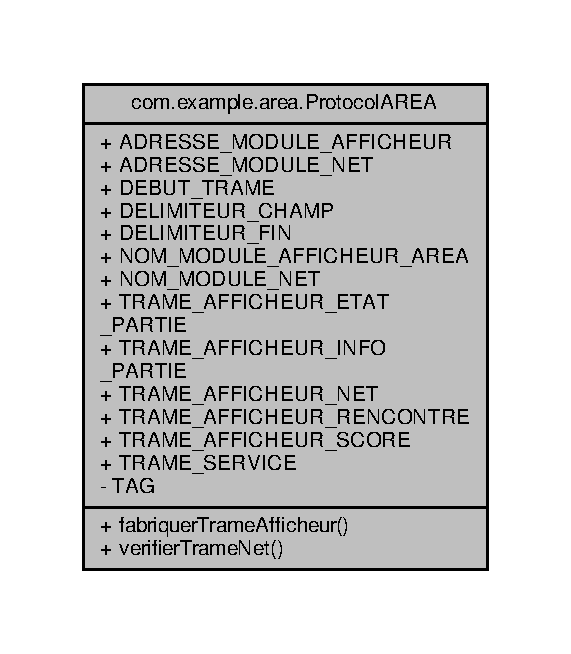
\includegraphics[width=274pt]{classcom_1_1example_1_1area_1_1_protocol_a_r_e_a__coll__graph}
\end{center}
\end{figure}
\subsubsection*{Fonctions membres publiques statiques}
\begin{DoxyCompactItemize}
\item 
static String \hyperlink{classcom_1_1example_1_1area_1_1_protocol_a_r_e_a_a3d4245d57e6b03b022e72c3ab9b2bc34}{fabriquer\+Trame\+Afficheur} (int type\+Trame, \hyperlink{classcom_1_1example_1_1area_1_1_partie}{Partie} partie)
\begin{DoxyCompactList}\small\item\em Méthode permettant de fabiquer les trames à destination du module Afficheur. \end{DoxyCompactList}\item 
static boolean \hyperlink{classcom_1_1example_1_1area_1_1_protocol_a_r_e_a_af675efbe6d33699aa34c01f6223fa711}{verifier\+Trame\+Net} (String trame)
\begin{DoxyCompactList}\small\item\em Méthode permettant de vérifier l\textquotesingle{}intégrité d\textquotesingle{}une trame N\+ET. \end{DoxyCompactList}\end{DoxyCompactItemize}
\subsubsection*{Attributs publics statiques}
\begin{DoxyCompactItemize}
\item 
static final String \hyperlink{classcom_1_1example_1_1area_1_1_protocol_a_r_e_a_a5f26c701d9ee639249d7f11e0b87b72d}{A\+D\+R\+E\+S\+S\+E\+\_\+\+M\+O\+D\+U\+L\+E\+\_\+\+A\+F\+F\+I\+C\+H\+E\+UR} = \char`\"{}D\+C\+:\+A6\+:32\+:52\+:7\+D\+:\+B5\char`\"{}
\item 
static final String \hyperlink{classcom_1_1example_1_1area_1_1_protocol_a_r_e_a_a57f9d1bae3c42517827ff0f193f0f36f}{A\+D\+R\+E\+S\+S\+E\+\_\+\+M\+O\+D\+U\+L\+E\+\_\+\+N\+ET} = \char`\"{}24\+:6\+F\+:28\+:7\+B\+:\+E1\+:06\char`\"{}
\item 
static final String \hyperlink{classcom_1_1example_1_1area_1_1_protocol_a_r_e_a_ad9aa917d162b8de3234b65ba294803ee}{D\+E\+B\+U\+T\+\_\+\+T\+R\+A\+ME} = \char`\"{}M\+O\+B\+I\+L\+E\+\_\+\+A\+R\+EA\char`\"{}
\item 
static final String \hyperlink{classcom_1_1example_1_1area_1_1_protocol_a_r_e_a_afec644c1c2a6563a0ee16a689044433c}{D\+E\+L\+I\+M\+I\+T\+E\+U\+R\+\_\+\+C\+H\+A\+MP} = \char`\"{};\char`\"{}
\item 
static final String \hyperlink{classcom_1_1example_1_1area_1_1_protocol_a_r_e_a_a77f13634749dc65bc24d98672ff7ba03}{D\+E\+L\+I\+M\+I\+T\+E\+U\+R\+\_\+\+F\+IN} = \char`\"{}\textbackslash{}r\textbackslash{}n\char`\"{}
\item 
static final String \hyperlink{classcom_1_1example_1_1area_1_1_protocol_a_r_e_a_afdfe4064c9e2d1c013bce83fd03c4326}{N\+O\+M\+\_\+\+M\+O\+D\+U\+L\+E\+\_\+\+A\+F\+F\+I\+C\+H\+E\+U\+R\+\_\+\+A\+R\+EA} = \char`\"{}A\+F\+F\+I\+C\+H\+E\+U\+R\+\_\+\+A\+R\+EA\char`\"{}
\item 
static final String \hyperlink{classcom_1_1example_1_1area_1_1_protocol_a_r_e_a_a77e082eb863a4839d0f1e885b31594e2}{N\+O\+M\+\_\+\+M\+O\+D\+U\+L\+E\+\_\+\+N\+ET} = \char`\"{}N\+E\+T\+\_\+\+A\+R\+EA\char`\"{}
\item 
static final int \hyperlink{classcom_1_1example_1_1area_1_1_protocol_a_r_e_a_a685ef5127e28517ca42fafb5cd6ba25a}{T\+R\+A\+M\+E\+\_\+\+A\+F\+F\+I\+C\+H\+E\+U\+R\+\_\+\+E\+T\+A\+T\+\_\+\+P\+A\+R\+T\+IE} = 3
\item 
static final int \hyperlink{classcom_1_1example_1_1area_1_1_protocol_a_r_e_a_a4f5be4d0653ad5f52ae5f5c673ec728d}{T\+R\+A\+M\+E\+\_\+\+A\+F\+F\+I\+C\+H\+E\+U\+R\+\_\+\+I\+N\+F\+O\+\_\+\+P\+A\+R\+T\+IE} = 1
\item 
static final int \hyperlink{classcom_1_1example_1_1area_1_1_protocol_a_r_e_a_a33bebef0a070831f8853b3f9e88532f2}{T\+R\+A\+M\+E\+\_\+\+A\+F\+F\+I\+C\+H\+E\+U\+R\+\_\+\+N\+ET} = 4
\item 
static final int \hyperlink{classcom_1_1example_1_1area_1_1_protocol_a_r_e_a_a6a896dcb5c52062dbeab426b93e566fc}{T\+R\+A\+M\+E\+\_\+\+A\+F\+F\+I\+C\+H\+E\+U\+R\+\_\+\+R\+E\+N\+C\+O\+N\+T\+RE} = 0
\item 
static final int \hyperlink{classcom_1_1example_1_1area_1_1_protocol_a_r_e_a_a63ba437bfc08504af2caaec99d61a230}{T\+R\+A\+M\+E\+\_\+\+A\+F\+F\+I\+C\+H\+E\+U\+R\+\_\+\+S\+C\+O\+RE} = 2
\item 
static final String \hyperlink{classcom_1_1example_1_1area_1_1_protocol_a_r_e_a_ab835cea072ee1568a285250debc1b3be}{T\+R\+A\+M\+E\+\_\+\+S\+E\+R\+V\+I\+CE} = \char`\"{}M\+O\+B\+I\+L\+E\+\_\+\+A\+R\+EA;S\+E\+R\+V\+I\+C\+E\textbackslash{}r\textbackslash{}n\char`\"{}
\end{DoxyCompactItemize}
\subsubsection*{Attributs privés statiques}
\begin{DoxyCompactItemize}
\item 
static final String \hyperlink{classcom_1_1example_1_1area_1_1_protocol_a_r_e_a_a4cc039bb2f3b605eb461b38dca05d22d}{T\+AG} = \char`\"{}\+\_\+\+Protocole\+A\+R\+EA\char`\"{}
\begin{DoxyCompactList}\small\item\em T\+AG pour les logs. \end{DoxyCompactList}\end{DoxyCompactItemize}


\subsubsection{Description détaillée}
Les détails du protocole A\+R\+EA. 

Définition à la ligne \hyperlink{_protocol_a_r_e_a_8java_source_l00019}{19} du fichier \hyperlink{_protocol_a_r_e_a_8java_source}{Protocol\+A\+R\+E\+A.\+java}.



\subsubsection{Documentation des fonctions membres}
\mbox{\Hypertarget{classcom_1_1example_1_1area_1_1_protocol_a_r_e_a_a3d4245d57e6b03b022e72c3ab9b2bc34}\label{classcom_1_1example_1_1area_1_1_protocol_a_r_e_a_a3d4245d57e6b03b022e72c3ab9b2bc34}} 
\index{com\+::example\+::area\+::\+Protocol\+A\+R\+EA@{com\+::example\+::area\+::\+Protocol\+A\+R\+EA}!fabriquer\+Trame\+Afficheur@{fabriquer\+Trame\+Afficheur}}
\index{fabriquer\+Trame\+Afficheur@{fabriquer\+Trame\+Afficheur}!com\+::example\+::area\+::\+Protocol\+A\+R\+EA@{com\+::example\+::area\+::\+Protocol\+A\+R\+EA}}
\paragraph{\texorpdfstring{fabriquer\+Trame\+Afficheur()}{fabriquerTrameAfficheur()}}
{\footnotesize\ttfamily static String com.\+example.\+area.\+Protocol\+A\+R\+E\+A.\+fabriquer\+Trame\+Afficheur (\begin{DoxyParamCaption}\item[{int}]{type\+Trame,  }\item[{\hyperlink{classcom_1_1example_1_1area_1_1_partie}{Partie}}]{partie }\end{DoxyParamCaption})\hspace{0.3cm}{\ttfamily [static]}}



Méthode permettant de fabiquer les trames à destination du module Afficheur. 

Utilitaires \begin{DoxyRefDesc}{A faire}
\item[\hyperlink{todo__todo000006}{A faire}]Compléter la méthode pour tous les types de trame \end{DoxyRefDesc}


M\+O\+B\+I\+L\+E\+\_\+\+A\+R\+EA;0;N\+O\+M\+\_\+\+C\+L\+U\+B\+\_\+A;N\+O\+M\+\_\+\+C\+L\+U\+B\+\_\+B~\newline


M\+O\+B\+I\+L\+E\+\_\+\+A\+R\+EA;1;I\+D\+\_\+\+P\+A\+R\+T\+IE;N\+O\+M\+\_\+\+J\+O\+U\+E\+U\+R\+\_\+A;P\+R\+E\+N\+O\+M\+\_\+\+J\+O\+U\+E\+U\+R\+\_\+A;\mbox{[}N\+O\+M\+\_\+\+D\+E\+U\+X\+I\+E\+M\+E\+\_\+\+J\+O\+U\+E\+U\+R\+\_\+A\mbox{]};\mbox{[}P\+R\+E\+N\+O\+M\+\_\+\+D\+E\+U\+X\+I\+E\+M\+E\+\_\+\+J\+O\+U\+E\+U\+R\+\_\+A\mbox{]};N\+O\+M\+\_\+\+J\+O\+U\+E\+U\+R\+\_\+B;P\+R\+E\+N\+O\+M\+\_\+\+J\+O\+U\+E\+U\+R\+\_\+B; \mbox{[}N\+O\+M\+\_\+\+D\+E\+U\+X\+I\+E\+M\+E\+\_\+\+J\+O\+U\+E\+U\+R\+\_\+B\mbox{]};\mbox{[}P\+R\+E\+N\+O\+M\+\_\+\+D\+E\+U\+X\+I\+E\+M\+E\+\_\+\+J\+O\+U\+E\+U\+R\+\_\+B\mbox{]}~\newline


M\+O\+B\+I\+L\+E\+\_\+\+A\+R\+EA;2;I\+D\+\_\+\+P\+A\+R\+T\+IE;P\+O\+I\+N\+T\+S\+\_\+\+J\+O\+U\+E\+U\+R\+\_\+A;P\+O\+I\+N\+T\+S\+\_\+\+J\+O\+U\+E\+U\+R\+\_\+B; N\+B\+\_\+\+M\+A\+N\+C\+H\+E\+S\+\_\+\+G\+A\+G\+N\+E\+E\+S\+\_\+\+J\+O\+U\+E\+U\+R\+\_\+A;N\+B\+\_\+\+M\+A\+N\+C\+H\+E\+S\+\_\+\+G\+A\+G\+N\+E\+E\+S\+\_\+\+J\+O\+U\+E\+U\+R\+\_\+B~\newline


M\+O\+B\+I\+L\+E\+\_\+\+A\+R\+EA;3;I\+D\+\_\+\+P\+A\+R\+T\+IE;E\+T\+AT~\newline
Le champs état peut prendre deux valeurs \+:
\begin{DoxyItemize}
\item La partie est en cours \+: E\+N\+\_\+\+C\+O\+U\+RS
\item La partie est en terminée \+: T\+E\+R\+M\+I\+N\+EE
\end{DoxyItemize}

M\+O\+B\+I\+L\+E\+\_\+\+A\+R\+EA;4;I\+D\+\_\+\+P\+A\+R\+T\+IE~\newline
 

Définition à la ligne \hyperlink{_protocol_a_r_e_a_8java_source_l00048}{48} du fichier \hyperlink{_protocol_a_r_e_a_8java_source}{Protocol\+A\+R\+E\+A.\+java}.



Références \hyperlink{_protocol_a_r_e_a_8java_source_l00031}{com.\+example.\+area.\+Protocol\+A\+R\+E\+A.\+D\+E\+B\+U\+T\+\_\+\+T\+R\+A\+ME}, \hyperlink{_protocol_a_r_e_a_8java_source_l00030}{com.\+example.\+area.\+Protocol\+A\+R\+E\+A.\+D\+E\+L\+I\+M\+I\+T\+E\+U\+R\+\_\+\+F\+IN}, \hyperlink{_partie_8java_source_l00036}{com.\+example.\+area.\+Partie.\+est\+Finie}, \hyperlink{_partie_8java_source_l00112}{com.\+example.\+area.\+Partie.\+get\+Id()}, \hyperlink{_partie_8java_source_l00064}{com.\+example.\+area.\+Partie.\+get\+Joueurs\+A()}, \hyperlink{_partie_8java_source_l00096}{com.\+example.\+area.\+Partie.\+get\+Manches\+Joueurs\+A()}, \hyperlink{_partie_8java_source_l00104}{com.\+example.\+area.\+Partie.\+get\+Manches\+Joueurs\+B()}, \hyperlink{_partie_8java_source_l00080}{com.\+example.\+area.\+Partie.\+get\+Points\+Joueurs\+A()}, \hyperlink{_partie_8java_source_l00088}{com.\+example.\+area.\+Partie.\+get\+Points\+Joueurs\+B()}, \hyperlink{_partie_8java_source_l00029}{com.\+example.\+area.\+Partie.\+P\+O\+S\+I\+T\+I\+O\+N\+\_\+\+D\+E\+U\+X\+I\+E\+M\+E\+\_\+\+J\+O\+U\+E\+UR}, \hyperlink{_partie_8java_source_l00028}{com.\+example.\+area.\+Partie.\+P\+O\+S\+I\+T\+I\+O\+N\+\_\+\+P\+R\+E\+M\+I\+E\+R\+\_\+\+J\+O\+U\+E\+UR}, \hyperlink{_protocol_a_r_e_a_8java_source_l00038}{com.\+example.\+area.\+Protocol\+A\+R\+E\+A.\+T\+R\+A\+M\+E\+\_\+\+A\+F\+F\+I\+C\+H\+E\+U\+R\+\_\+\+E\+T\+A\+T\+\_\+\+P\+A\+R\+T\+IE}, \hyperlink{_protocol_a_r_e_a_8java_source_l00036}{com.\+example.\+area.\+Protocol\+A\+R\+E\+A.\+T\+R\+A\+M\+E\+\_\+\+A\+F\+F\+I\+C\+H\+E\+U\+R\+\_\+\+I\+N\+F\+O\+\_\+\+P\+A\+R\+T\+IE}, \hyperlink{_protocol_a_r_e_a_8java_source_l00039}{com.\+example.\+area.\+Protocol\+A\+R\+E\+A.\+T\+R\+A\+M\+E\+\_\+\+A\+F\+F\+I\+C\+H\+E\+U\+R\+\_\+\+N\+ET}, \hyperlink{_protocol_a_r_e_a_8java_source_l00035}{com.\+example.\+area.\+Protocol\+A\+R\+E\+A.\+T\+R\+A\+M\+E\+\_\+\+A\+F\+F\+I\+C\+H\+E\+U\+R\+\_\+\+R\+E\+N\+C\+O\+N\+T\+RE}, et \hyperlink{_protocol_a_r_e_a_8java_source_l00037}{com.\+example.\+area.\+Protocol\+A\+R\+E\+A.\+T\+R\+A\+M\+E\+\_\+\+A\+F\+F\+I\+C\+H\+E\+U\+R\+\_\+\+S\+C\+O\+RE}.



Référencé par \hyperlink{_i_h_m_gestion_partie_8java_source_l00346}{com.\+example.\+area.\+I\+H\+M\+Gestion\+Partie.\+connecter\+Boutons()}, \hyperlink{_i_h_m_gestion_partie_8java_source_l00291}{com.\+example.\+area.\+I\+H\+M\+Gestion\+Partie.\+initialiser\+Handler()}, et \hyperlink{_i_h_m_gestion_partie_8java_source_l00329}{com.\+example.\+area.\+I\+H\+M\+Gestion\+Partie.\+initialiser\+Liaison\+Bluetooth()}.


\begin{DoxyCode}
00049     \{
00050         String trame = \hyperlink{classcom_1_1example_1_1area_1_1_protocol_a_r_e_a_ad9aa917d162b8de3234b65ba294803ee}{DEBUT\_TRAME};
00051 
00055         \textcolor{keywordflow}{switch} (typeTrame)
00056         \{
00057             \textcolor{keywordflow}{case} \hyperlink{classcom_1_1example_1_1area_1_1_protocol_a_r_e_a_a6a896dcb5c52062dbeab426b93e566fc}{TRAME\_AFFICHEUR\_RENCONTRE}:
00061                 \textcolor{keywordflow}{break};
00062             \textcolor{keywordflow}{case} \hyperlink{classcom_1_1example_1_1area_1_1_protocol_a_r_e_a_a4f5be4d0653ad5f52ae5f5c673ec728d}{TRAME\_AFFICHEUR\_INFO\_PARTIE}:
00067                 Vector<Joueur> joueursA = partie.getJoueursA();
00068                 Vector<Joueur> joueursB = partie.getJoueursA();
00069                 \textcolor{keywordflow}{if} (joueursA.size() > 1)
00070                     trame += \hyperlink{classcom_1_1example_1_1area_1_1_protocol_a_r_e_a_afec644c1c2a6563a0ee16a689044433c}{DELIMITEUR\_CHAMP} + 
      \hyperlink{classcom_1_1example_1_1area_1_1_protocol_a_r_e_a_a4f5be4d0653ad5f52ae5f5c673ec728d}{TRAME\_AFFICHEUR\_INFO\_PARTIE} + joueursA.elementAt(Partie.POSITION\_PREMIER\_JOUEUR)
      .getNom() + \hyperlink{classcom_1_1example_1_1area_1_1_protocol_a_r_e_a_afec644c1c2a6563a0ee16a689044433c}{DELIMITEUR\_CHAMP} +
00071                             joueursA.elementAt(Partie.POSITION\_PREMIER\_JOUEUR).getPrenom() + 
      \hyperlink{classcom_1_1example_1_1area_1_1_protocol_a_r_e_a_afec644c1c2a6563a0ee16a689044433c}{DELIMITEUR\_CHAMP} + joueursA.elementAt(Partie.POSITION\_DEUXIEME\_JOUEUR).getNom() + 
      \hyperlink{classcom_1_1example_1_1area_1_1_protocol_a_r_e_a_afec644c1c2a6563a0ee16a689044433c}{DELIMITEUR\_CHAMP} +
00072                             joueursA.elementAt(Partie.POSITION\_DEUXIEME\_JOUEUR).getPrenom() + 
      \hyperlink{classcom_1_1example_1_1area_1_1_protocol_a_r_e_a_afec644c1c2a6563a0ee16a689044433c}{DELIMITEUR\_CHAMP} + joueursB.elementAt(Partie.POSITION\_PREMIER\_JOUEUR).getNom() + 
      \hyperlink{classcom_1_1example_1_1area_1_1_protocol_a_r_e_a_afec644c1c2a6563a0ee16a689044433c}{DELIMITEUR\_CHAMP} +
00073                             joueursB.elementAt(Partie.POSITION\_PREMIER\_JOUEUR).getPrenom() + 
      \hyperlink{classcom_1_1example_1_1area_1_1_protocol_a_r_e_a_afec644c1c2a6563a0ee16a689044433c}{DELIMITEUR\_CHAMP} + joueursB.elementAt(Partie.POSITION\_DEUXIEME\_JOUEUR).getNom() + 
      \hyperlink{classcom_1_1example_1_1area_1_1_protocol_a_r_e_a_afec644c1c2a6563a0ee16a689044433c}{DELIMITEUR\_CHAMP} +
00074                             joueursB.elementAt(Partie.POSITION\_DEUXIEME\_JOUEUR).getPrenom() + 
      \hyperlink{classcom_1_1example_1_1area_1_1_protocol_a_r_e_a_a77f13634749dc65bc24d98672ff7ba03}{DELIMITEUR\_FIN};
00075                 \textcolor{keywordflow}{else}
00076                     trame += \hyperlink{classcom_1_1example_1_1area_1_1_protocol_a_r_e_a_afec644c1c2a6563a0ee16a689044433c}{DELIMITEUR\_CHAMP} + 
      \hyperlink{classcom_1_1example_1_1area_1_1_protocol_a_r_e_a_a4f5be4d0653ad5f52ae5f5c673ec728d}{TRAME\_AFFICHEUR\_INFO\_PARTIE} + joueursA.elementAt(Partie.POSITION\_PREMIER\_JOUEUR)
      .getNom() + \hyperlink{classcom_1_1example_1_1area_1_1_protocol_a_r_e_a_afec644c1c2a6563a0ee16a689044433c}{DELIMITEUR\_CHAMP} +
00077                             joueursA.elementAt(Partie.POSITION\_PREMIER\_JOUEUR).getPrenom() + 
      \hyperlink{classcom_1_1example_1_1area_1_1_protocol_a_r_e_a_afec644c1c2a6563a0ee16a689044433c}{DELIMITEUR\_CHAMP} + joueursB.elementAt(Partie.POSITION\_PREMIER\_JOUEUR).getNom() + 
      \hyperlink{classcom_1_1example_1_1area_1_1_protocol_a_r_e_a_afec644c1c2a6563a0ee16a689044433c}{DELIMITEUR\_CHAMP} +
00078                             joueursB.elementAt(Partie.POSITION\_PREMIER\_JOUEUR).getPrenom() + 
      \hyperlink{classcom_1_1example_1_1area_1_1_protocol_a_r_e_a_a77f13634749dc65bc24d98672ff7ba03}{DELIMITEUR\_FIN};
00079                 \textcolor{keywordflow}{break};
00080             \textcolor{keywordflow}{case} \hyperlink{classcom_1_1example_1_1area_1_1_protocol_a_r_e_a_a63ba437bfc08504af2caaec99d61a230}{TRAME\_AFFICHEUR\_SCORE}:
00085                 trame += \hyperlink{classcom_1_1example_1_1area_1_1_protocol_a_r_e_a_afec644c1c2a6563a0ee16a689044433c}{DELIMITEUR\_CHAMP} + 
      \hyperlink{classcom_1_1example_1_1area_1_1_protocol_a_r_e_a_a63ba437bfc08504af2caaec99d61a230}{TRAME\_AFFICHEUR\_SCORE} + \hyperlink{classcom_1_1example_1_1area_1_1_protocol_a_r_e_a_afec644c1c2a6563a0ee16a689044433c}{DELIMITEUR\_CHAMP} + partie.getId() + 
      \hyperlink{classcom_1_1example_1_1area_1_1_protocol_a_r_e_a_afec644c1c2a6563a0ee16a689044433c}{DELIMITEUR\_CHAMP} + partie.getPointsJoueursA() +
00086                         \hyperlink{classcom_1_1example_1_1area_1_1_protocol_a_r_e_a_afec644c1c2a6563a0ee16a689044433c}{DELIMITEUR\_CHAMP} + partie.getPointsJoueursB() + 
      \hyperlink{classcom_1_1example_1_1area_1_1_protocol_a_r_e_a_afec644c1c2a6563a0ee16a689044433c}{DELIMITEUR\_CHAMP} + partie.getManchesJoueursA() + 
      \hyperlink{classcom_1_1example_1_1area_1_1_protocol_a_r_e_a_afec644c1c2a6563a0ee16a689044433c}{DELIMITEUR\_CHAMP} +
00087                         partie.getManchesJoueursB() + \hyperlink{classcom_1_1example_1_1area_1_1_protocol_a_r_e_a_a77f13634749dc65bc24d98672ff7ba03}{DELIMITEUR\_FIN};
00088                 \textcolor{keywordflow}{break};
00089             \textcolor{keywordflow}{case} \hyperlink{classcom_1_1example_1_1area_1_1_protocol_a_r_e_a_a685ef5127e28517ca42fafb5cd6ba25a}{TRAME\_AFFICHEUR\_ETAT\_PARTIE}:
00096                 String etat = \textcolor{stringliteral}{"EN\_COURS"};
00097                 \textcolor{keywordflow}{if} (partie.estFinie())
00098                     etat = \textcolor{stringliteral}{"TERMINEE"};
00099                 trame += \hyperlink{classcom_1_1example_1_1area_1_1_protocol_a_r_e_a_afec644c1c2a6563a0ee16a689044433c}{DELIMITEUR\_CHAMP} + 
      \hyperlink{classcom_1_1example_1_1area_1_1_protocol_a_r_e_a_a685ef5127e28517ca42fafb5cd6ba25a}{TRAME\_AFFICHEUR\_ETAT\_PARTIE} + \hyperlink{classcom_1_1example_1_1area_1_1_protocol_a_r_e_a_afec644c1c2a6563a0ee16a689044433c}{DELIMITEUR\_CHAMP} + partie.getId() 
      + \hyperlink{classcom_1_1example_1_1area_1_1_protocol_a_r_e_a_afec644c1c2a6563a0ee16a689044433c}{DELIMITEUR\_CHAMP} + etat + \hyperlink{classcom_1_1example_1_1area_1_1_protocol_a_r_e_a_a77f13634749dc65bc24d98672ff7ba03}{DELIMITEUR\_FIN};
00100                 \textcolor{keywordflow}{break};
00101             \textcolor{keywordflow}{case} \hyperlink{classcom_1_1example_1_1area_1_1_protocol_a_r_e_a_a33bebef0a070831f8853b3f9e88532f2}{TRAME\_AFFICHEUR\_NET}:
00105                 trame += \hyperlink{classcom_1_1example_1_1area_1_1_protocol_a_r_e_a_afec644c1c2a6563a0ee16a689044433c}{DELIMITEUR\_CHAMP} + \hyperlink{classcom_1_1example_1_1area_1_1_protocol_a_r_e_a_a33bebef0a070831f8853b3f9e88532f2}{TRAME\_AFFICHEUR\_NET} + 
      \hyperlink{classcom_1_1example_1_1area_1_1_protocol_a_r_e_a_afec644c1c2a6563a0ee16a689044433c}{DELIMITEUR\_CHAMP} + partie.getId() + \hyperlink{classcom_1_1example_1_1area_1_1_protocol_a_r_e_a_a77f13634749dc65bc24d98672ff7ba03}{DELIMITEUR\_FIN};
00106                 \textcolor{keywordflow}{break};
00107         \}
00108 
00109         Log.d(\hyperlink{classcom_1_1example_1_1area_1_1_protocol_a_r_e_a_a4cc039bb2f3b605eb461b38dca05d22d}{TAG}, \textcolor{stringliteral}{"fabriquerTrameAfficheur() trame = "} + trame);
00110 
00111         \textcolor{keywordflow}{return} trame;
00112     \}
\end{DoxyCode}
\mbox{\Hypertarget{classcom_1_1example_1_1area_1_1_protocol_a_r_e_a_af675efbe6d33699aa34c01f6223fa711}\label{classcom_1_1example_1_1area_1_1_protocol_a_r_e_a_af675efbe6d33699aa34c01f6223fa711}} 
\index{com\+::example\+::area\+::\+Protocol\+A\+R\+EA@{com\+::example\+::area\+::\+Protocol\+A\+R\+EA}!verifier\+Trame\+Net@{verifier\+Trame\+Net}}
\index{verifier\+Trame\+Net@{verifier\+Trame\+Net}!com\+::example\+::area\+::\+Protocol\+A\+R\+EA@{com\+::example\+::area\+::\+Protocol\+A\+R\+EA}}
\paragraph{\texorpdfstring{verifier\+Trame\+Net()}{verifierTrameNet()}}
{\footnotesize\ttfamily static boolean com.\+example.\+area.\+Protocol\+A\+R\+E\+A.\+verifier\+Trame\+Net (\begin{DoxyParamCaption}\item[{String}]{trame }\end{DoxyParamCaption})\hspace{0.3cm}{\ttfamily [static]}}



Méthode permettant de vérifier l\textquotesingle{}intégrité d\textquotesingle{}une trame N\+ET. 



Définition à la ligne \hyperlink{_protocol_a_r_e_a_8java_source_l00117}{117} du fichier \hyperlink{_protocol_a_r_e_a_8java_source}{Protocol\+A\+R\+E\+A.\+java}.



Référencé par \hyperlink{_i_h_m_gestion_partie_8java_source_l00291}{com.\+example.\+area.\+I\+H\+M\+Gestion\+Partie.\+initialiser\+Handler()}.


\begin{DoxyCode}
00118     \{
00119         \textcolor{keywordflow}{if} (trame.startsWith(\textcolor{stringliteral}{"NET\_AREA"}) && trame.contains(\textcolor{stringliteral}{"NET"}))
00120         \{
00121             \textcolor{keywordflow}{return} \textcolor{keyword}{true};
00122         \}
00123         \textcolor{keywordflow}{return} \textcolor{keyword}{false};
00124     \}
\end{DoxyCode}


\subsubsection{Documentation des données membres}
\mbox{\Hypertarget{classcom_1_1example_1_1area_1_1_protocol_a_r_e_a_a5f26c701d9ee639249d7f11e0b87b72d}\label{classcom_1_1example_1_1area_1_1_protocol_a_r_e_a_a5f26c701d9ee639249d7f11e0b87b72d}} 
\index{com\+::example\+::area\+::\+Protocol\+A\+R\+EA@{com\+::example\+::area\+::\+Protocol\+A\+R\+EA}!A\+D\+R\+E\+S\+S\+E\+\_\+\+M\+O\+D\+U\+L\+E\+\_\+\+A\+F\+F\+I\+C\+H\+E\+UR@{A\+D\+R\+E\+S\+S\+E\+\_\+\+M\+O\+D\+U\+L\+E\+\_\+\+A\+F\+F\+I\+C\+H\+E\+UR}}
\index{A\+D\+R\+E\+S\+S\+E\+\_\+\+M\+O\+D\+U\+L\+E\+\_\+\+A\+F\+F\+I\+C\+H\+E\+UR@{A\+D\+R\+E\+S\+S\+E\+\_\+\+M\+O\+D\+U\+L\+E\+\_\+\+A\+F\+F\+I\+C\+H\+E\+UR}!com\+::example\+::area\+::\+Protocol\+A\+R\+EA@{com\+::example\+::area\+::\+Protocol\+A\+R\+EA}}
\paragraph{\texorpdfstring{A\+D\+R\+E\+S\+S\+E\+\_\+\+M\+O\+D\+U\+L\+E\+\_\+\+A\+F\+F\+I\+C\+H\+E\+UR}{ADRESSE\_MODULE\_AFFICHEUR}}
{\footnotesize\ttfamily final String com.\+example.\+area.\+Protocol\+A\+R\+E\+A.\+A\+D\+R\+E\+S\+S\+E\+\_\+\+M\+O\+D\+U\+L\+E\+\_\+\+A\+F\+F\+I\+C\+H\+E\+UR = \char`\"{}D\+C\+:\+A6\+:32\+:52\+:7\+D\+:\+B5\char`\"{}\hspace{0.3cm}{\ttfamily [static]}}



Définition à la ligne \hyperlink{_protocol_a_r_e_a_8java_source_l00028}{28} du fichier \hyperlink{_protocol_a_r_e_a_8java_source}{Protocol\+A\+R\+E\+A.\+java}.



Référencé par \hyperlink{_i_h_m_gestion_partie_8java_source_l00329}{com.\+example.\+area.\+I\+H\+M\+Gestion\+Partie.\+initialiser\+Liaison\+Bluetooth()}.

\mbox{\Hypertarget{classcom_1_1example_1_1area_1_1_protocol_a_r_e_a_a57f9d1bae3c42517827ff0f193f0f36f}\label{classcom_1_1example_1_1area_1_1_protocol_a_r_e_a_a57f9d1bae3c42517827ff0f193f0f36f}} 
\index{com\+::example\+::area\+::\+Protocol\+A\+R\+EA@{com\+::example\+::area\+::\+Protocol\+A\+R\+EA}!A\+D\+R\+E\+S\+S\+E\+\_\+\+M\+O\+D\+U\+L\+E\+\_\+\+N\+ET@{A\+D\+R\+E\+S\+S\+E\+\_\+\+M\+O\+D\+U\+L\+E\+\_\+\+N\+ET}}
\index{A\+D\+R\+E\+S\+S\+E\+\_\+\+M\+O\+D\+U\+L\+E\+\_\+\+N\+ET@{A\+D\+R\+E\+S\+S\+E\+\_\+\+M\+O\+D\+U\+L\+E\+\_\+\+N\+ET}!com\+::example\+::area\+::\+Protocol\+A\+R\+EA@{com\+::example\+::area\+::\+Protocol\+A\+R\+EA}}
\paragraph{\texorpdfstring{A\+D\+R\+E\+S\+S\+E\+\_\+\+M\+O\+D\+U\+L\+E\+\_\+\+N\+ET}{ADRESSE\_MODULE\_NET}}
{\footnotesize\ttfamily final String com.\+example.\+area.\+Protocol\+A\+R\+E\+A.\+A\+D\+R\+E\+S\+S\+E\+\_\+\+M\+O\+D\+U\+L\+E\+\_\+\+N\+ET = \char`\"{}24\+:6\+F\+:28\+:7\+B\+:\+E1\+:06\char`\"{}\hspace{0.3cm}{\ttfamily [static]}}



Définition à la ligne \hyperlink{_protocol_a_r_e_a_8java_source_l00027}{27} du fichier \hyperlink{_protocol_a_r_e_a_8java_source}{Protocol\+A\+R\+E\+A.\+java}.



Référencé par \hyperlink{_i_h_m_gestion_partie_8java_source_l00329}{com.\+example.\+area.\+I\+H\+M\+Gestion\+Partie.\+initialiser\+Liaison\+Bluetooth()}.

\mbox{\Hypertarget{classcom_1_1example_1_1area_1_1_protocol_a_r_e_a_ad9aa917d162b8de3234b65ba294803ee}\label{classcom_1_1example_1_1area_1_1_protocol_a_r_e_a_ad9aa917d162b8de3234b65ba294803ee}} 
\index{com\+::example\+::area\+::\+Protocol\+A\+R\+EA@{com\+::example\+::area\+::\+Protocol\+A\+R\+EA}!D\+E\+B\+U\+T\+\_\+\+T\+R\+A\+ME@{D\+E\+B\+U\+T\+\_\+\+T\+R\+A\+ME}}
\index{D\+E\+B\+U\+T\+\_\+\+T\+R\+A\+ME@{D\+E\+B\+U\+T\+\_\+\+T\+R\+A\+ME}!com\+::example\+::area\+::\+Protocol\+A\+R\+EA@{com\+::example\+::area\+::\+Protocol\+A\+R\+EA}}
\paragraph{\texorpdfstring{D\+E\+B\+U\+T\+\_\+\+T\+R\+A\+ME}{DEBUT\_TRAME}}
{\footnotesize\ttfamily final String com.\+example.\+area.\+Protocol\+A\+R\+E\+A.\+D\+E\+B\+U\+T\+\_\+\+T\+R\+A\+ME = \char`\"{}M\+O\+B\+I\+L\+E\+\_\+\+A\+R\+EA\char`\"{}\hspace{0.3cm}{\ttfamily [static]}}



Définition à la ligne \hyperlink{_protocol_a_r_e_a_8java_source_l00031}{31} du fichier \hyperlink{_protocol_a_r_e_a_8java_source}{Protocol\+A\+R\+E\+A.\+java}.



Référencé par \hyperlink{_protocol_a_r_e_a_8java_source_l00048}{com.\+example.\+area.\+Protocol\+A\+R\+E\+A.\+fabriquer\+Trame\+Afficheur()}.

\mbox{\Hypertarget{classcom_1_1example_1_1area_1_1_protocol_a_r_e_a_afec644c1c2a6563a0ee16a689044433c}\label{classcom_1_1example_1_1area_1_1_protocol_a_r_e_a_afec644c1c2a6563a0ee16a689044433c}} 
\index{com\+::example\+::area\+::\+Protocol\+A\+R\+EA@{com\+::example\+::area\+::\+Protocol\+A\+R\+EA}!D\+E\+L\+I\+M\+I\+T\+E\+U\+R\+\_\+\+C\+H\+A\+MP@{D\+E\+L\+I\+M\+I\+T\+E\+U\+R\+\_\+\+C\+H\+A\+MP}}
\index{D\+E\+L\+I\+M\+I\+T\+E\+U\+R\+\_\+\+C\+H\+A\+MP@{D\+E\+L\+I\+M\+I\+T\+E\+U\+R\+\_\+\+C\+H\+A\+MP}!com\+::example\+::area\+::\+Protocol\+A\+R\+EA@{com\+::example\+::area\+::\+Protocol\+A\+R\+EA}}
\paragraph{\texorpdfstring{D\+E\+L\+I\+M\+I\+T\+E\+U\+R\+\_\+\+C\+H\+A\+MP}{DELIMITEUR\_CHAMP}}
{\footnotesize\ttfamily final String com.\+example.\+area.\+Protocol\+A\+R\+E\+A.\+D\+E\+L\+I\+M\+I\+T\+E\+U\+R\+\_\+\+C\+H\+A\+MP = \char`\"{};\char`\"{}\hspace{0.3cm}{\ttfamily [static]}}



Définition à la ligne \hyperlink{_protocol_a_r_e_a_8java_source_l00029}{29} du fichier \hyperlink{_protocol_a_r_e_a_8java_source}{Protocol\+A\+R\+E\+A.\+java}.

\mbox{\Hypertarget{classcom_1_1example_1_1area_1_1_protocol_a_r_e_a_a77f13634749dc65bc24d98672ff7ba03}\label{classcom_1_1example_1_1area_1_1_protocol_a_r_e_a_a77f13634749dc65bc24d98672ff7ba03}} 
\index{com\+::example\+::area\+::\+Protocol\+A\+R\+EA@{com\+::example\+::area\+::\+Protocol\+A\+R\+EA}!D\+E\+L\+I\+M\+I\+T\+E\+U\+R\+\_\+\+F\+IN@{D\+E\+L\+I\+M\+I\+T\+E\+U\+R\+\_\+\+F\+IN}}
\index{D\+E\+L\+I\+M\+I\+T\+E\+U\+R\+\_\+\+F\+IN@{D\+E\+L\+I\+M\+I\+T\+E\+U\+R\+\_\+\+F\+IN}!com\+::example\+::area\+::\+Protocol\+A\+R\+EA@{com\+::example\+::area\+::\+Protocol\+A\+R\+EA}}
\paragraph{\texorpdfstring{D\+E\+L\+I\+M\+I\+T\+E\+U\+R\+\_\+\+F\+IN}{DELIMITEUR\_FIN}}
{\footnotesize\ttfamily final String com.\+example.\+area.\+Protocol\+A\+R\+E\+A.\+D\+E\+L\+I\+M\+I\+T\+E\+U\+R\+\_\+\+F\+IN = \char`\"{}\textbackslash{}r\textbackslash{}n\char`\"{}\hspace{0.3cm}{\ttfamily [static]}}



Définition à la ligne \hyperlink{_protocol_a_r_e_a_8java_source_l00030}{30} du fichier \hyperlink{_protocol_a_r_e_a_8java_source}{Protocol\+A\+R\+E\+A.\+java}.



Référencé par \hyperlink{_protocol_a_r_e_a_8java_source_l00048}{com.\+example.\+area.\+Protocol\+A\+R\+E\+A.\+fabriquer\+Trame\+Afficheur()}.

\mbox{\Hypertarget{classcom_1_1example_1_1area_1_1_protocol_a_r_e_a_afdfe4064c9e2d1c013bce83fd03c4326}\label{classcom_1_1example_1_1area_1_1_protocol_a_r_e_a_afdfe4064c9e2d1c013bce83fd03c4326}} 
\index{com\+::example\+::area\+::\+Protocol\+A\+R\+EA@{com\+::example\+::area\+::\+Protocol\+A\+R\+EA}!N\+O\+M\+\_\+\+M\+O\+D\+U\+L\+E\+\_\+\+A\+F\+F\+I\+C\+H\+E\+U\+R\+\_\+\+A\+R\+EA@{N\+O\+M\+\_\+\+M\+O\+D\+U\+L\+E\+\_\+\+A\+F\+F\+I\+C\+H\+E\+U\+R\+\_\+\+A\+R\+EA}}
\index{N\+O\+M\+\_\+\+M\+O\+D\+U\+L\+E\+\_\+\+A\+F\+F\+I\+C\+H\+E\+U\+R\+\_\+\+A\+R\+EA@{N\+O\+M\+\_\+\+M\+O\+D\+U\+L\+E\+\_\+\+A\+F\+F\+I\+C\+H\+E\+U\+R\+\_\+\+A\+R\+EA}!com\+::example\+::area\+::\+Protocol\+A\+R\+EA@{com\+::example\+::area\+::\+Protocol\+A\+R\+EA}}
\paragraph{\texorpdfstring{N\+O\+M\+\_\+\+M\+O\+D\+U\+L\+E\+\_\+\+A\+F\+F\+I\+C\+H\+E\+U\+R\+\_\+\+A\+R\+EA}{NOM\_MODULE\_AFFICHEUR\_AREA}}
{\footnotesize\ttfamily final String com.\+example.\+area.\+Protocol\+A\+R\+E\+A.\+N\+O\+M\+\_\+\+M\+O\+D\+U\+L\+E\+\_\+\+A\+F\+F\+I\+C\+H\+E\+U\+R\+\_\+\+A\+R\+EA = \char`\"{}A\+F\+F\+I\+C\+H\+E\+U\+R\+\_\+\+A\+R\+EA\char`\"{}\hspace{0.3cm}{\ttfamily [static]}}



Définition à la ligne \hyperlink{_protocol_a_r_e_a_8java_source_l00026}{26} du fichier \hyperlink{_protocol_a_r_e_a_8java_source}{Protocol\+A\+R\+E\+A.\+java}.



Référencé par \hyperlink{_i_h_m_gestion_partie_8java_source_l00329}{com.\+example.\+area.\+I\+H\+M\+Gestion\+Partie.\+initialiser\+Liaison\+Bluetooth()}.

\mbox{\Hypertarget{classcom_1_1example_1_1area_1_1_protocol_a_r_e_a_a77e082eb863a4839d0f1e885b31594e2}\label{classcom_1_1example_1_1area_1_1_protocol_a_r_e_a_a77e082eb863a4839d0f1e885b31594e2}} 
\index{com\+::example\+::area\+::\+Protocol\+A\+R\+EA@{com\+::example\+::area\+::\+Protocol\+A\+R\+EA}!N\+O\+M\+\_\+\+M\+O\+D\+U\+L\+E\+\_\+\+N\+ET@{N\+O\+M\+\_\+\+M\+O\+D\+U\+L\+E\+\_\+\+N\+ET}}
\index{N\+O\+M\+\_\+\+M\+O\+D\+U\+L\+E\+\_\+\+N\+ET@{N\+O\+M\+\_\+\+M\+O\+D\+U\+L\+E\+\_\+\+N\+ET}!com\+::example\+::area\+::\+Protocol\+A\+R\+EA@{com\+::example\+::area\+::\+Protocol\+A\+R\+EA}}
\paragraph{\texorpdfstring{N\+O\+M\+\_\+\+M\+O\+D\+U\+L\+E\+\_\+\+N\+ET}{NOM\_MODULE\_NET}}
{\footnotesize\ttfamily final String com.\+example.\+area.\+Protocol\+A\+R\+E\+A.\+N\+O\+M\+\_\+\+M\+O\+D\+U\+L\+E\+\_\+\+N\+ET = \char`\"{}N\+E\+T\+\_\+\+A\+R\+EA\char`\"{}\hspace{0.3cm}{\ttfamily [static]}}



Définition à la ligne \hyperlink{_protocol_a_r_e_a_8java_source_l00025}{25} du fichier \hyperlink{_protocol_a_r_e_a_8java_source}{Protocol\+A\+R\+E\+A.\+java}.



Référencé par \hyperlink{_i_h_m_gestion_partie_8java_source_l00488}{com.\+example.\+area.\+I\+H\+M\+Gestion\+Partie.\+afficher\+Etat\+Connexion\+Bluetooth()}, et \hyperlink{_i_h_m_gestion_partie_8java_source_l00329}{com.\+example.\+area.\+I\+H\+M\+Gestion\+Partie.\+initialiser\+Liaison\+Bluetooth()}.

\mbox{\Hypertarget{classcom_1_1example_1_1area_1_1_protocol_a_r_e_a_a4cc039bb2f3b605eb461b38dca05d22d}\label{classcom_1_1example_1_1area_1_1_protocol_a_r_e_a_a4cc039bb2f3b605eb461b38dca05d22d}} 
\index{com\+::example\+::area\+::\+Protocol\+A\+R\+EA@{com\+::example\+::area\+::\+Protocol\+A\+R\+EA}!T\+AG@{T\+AG}}
\index{T\+AG@{T\+AG}!com\+::example\+::area\+::\+Protocol\+A\+R\+EA@{com\+::example\+::area\+::\+Protocol\+A\+R\+EA}}
\paragraph{\texorpdfstring{T\+AG}{TAG}}
{\footnotesize\ttfamily final String com.\+example.\+area.\+Protocol\+A\+R\+E\+A.\+T\+AG = \char`\"{}\+\_\+\+Protocole\+A\+R\+EA\char`\"{}\hspace{0.3cm}{\ttfamily [static]}, {\ttfamily [private]}}



T\+AG pour les logs. 

Constantes 

Définition à la ligne \hyperlink{_protocol_a_r_e_a_8java_source_l00024}{24} du fichier \hyperlink{_protocol_a_r_e_a_8java_source}{Protocol\+A\+R\+E\+A.\+java}.

\mbox{\Hypertarget{classcom_1_1example_1_1area_1_1_protocol_a_r_e_a_a685ef5127e28517ca42fafb5cd6ba25a}\label{classcom_1_1example_1_1area_1_1_protocol_a_r_e_a_a685ef5127e28517ca42fafb5cd6ba25a}} 
\index{com\+::example\+::area\+::\+Protocol\+A\+R\+EA@{com\+::example\+::area\+::\+Protocol\+A\+R\+EA}!T\+R\+A\+M\+E\+\_\+\+A\+F\+F\+I\+C\+H\+E\+U\+R\+\_\+\+E\+T\+A\+T\+\_\+\+P\+A\+R\+T\+IE@{T\+R\+A\+M\+E\+\_\+\+A\+F\+F\+I\+C\+H\+E\+U\+R\+\_\+\+E\+T\+A\+T\+\_\+\+P\+A\+R\+T\+IE}}
\index{T\+R\+A\+M\+E\+\_\+\+A\+F\+F\+I\+C\+H\+E\+U\+R\+\_\+\+E\+T\+A\+T\+\_\+\+P\+A\+R\+T\+IE@{T\+R\+A\+M\+E\+\_\+\+A\+F\+F\+I\+C\+H\+E\+U\+R\+\_\+\+E\+T\+A\+T\+\_\+\+P\+A\+R\+T\+IE}!com\+::example\+::area\+::\+Protocol\+A\+R\+EA@{com\+::example\+::area\+::\+Protocol\+A\+R\+EA}}
\paragraph{\texorpdfstring{T\+R\+A\+M\+E\+\_\+\+A\+F\+F\+I\+C\+H\+E\+U\+R\+\_\+\+E\+T\+A\+T\+\_\+\+P\+A\+R\+T\+IE}{TRAME\_AFFICHEUR\_ETAT\_PARTIE}}
{\footnotesize\ttfamily final int com.\+example.\+area.\+Protocol\+A\+R\+E\+A.\+T\+R\+A\+M\+E\+\_\+\+A\+F\+F\+I\+C\+H\+E\+U\+R\+\_\+\+E\+T\+A\+T\+\_\+\+P\+A\+R\+T\+IE = 3\hspace{0.3cm}{\ttfamily [static]}}



Définition à la ligne \hyperlink{_protocol_a_r_e_a_8java_source_l00038}{38} du fichier \hyperlink{_protocol_a_r_e_a_8java_source}{Protocol\+A\+R\+E\+A.\+java}.



Référencé par \hyperlink{_protocol_a_r_e_a_8java_source_l00048}{com.\+example.\+area.\+Protocol\+A\+R\+E\+A.\+fabriquer\+Trame\+Afficheur()}, et \hyperlink{_i_h_m_gestion_partie_8java_source_l00329}{com.\+example.\+area.\+I\+H\+M\+Gestion\+Partie.\+initialiser\+Liaison\+Bluetooth()}.

\mbox{\Hypertarget{classcom_1_1example_1_1area_1_1_protocol_a_r_e_a_a4f5be4d0653ad5f52ae5f5c673ec728d}\label{classcom_1_1example_1_1area_1_1_protocol_a_r_e_a_a4f5be4d0653ad5f52ae5f5c673ec728d}} 
\index{com\+::example\+::area\+::\+Protocol\+A\+R\+EA@{com\+::example\+::area\+::\+Protocol\+A\+R\+EA}!T\+R\+A\+M\+E\+\_\+\+A\+F\+F\+I\+C\+H\+E\+U\+R\+\_\+\+I\+N\+F\+O\+\_\+\+P\+A\+R\+T\+IE@{T\+R\+A\+M\+E\+\_\+\+A\+F\+F\+I\+C\+H\+E\+U\+R\+\_\+\+I\+N\+F\+O\+\_\+\+P\+A\+R\+T\+IE}}
\index{T\+R\+A\+M\+E\+\_\+\+A\+F\+F\+I\+C\+H\+E\+U\+R\+\_\+\+I\+N\+F\+O\+\_\+\+P\+A\+R\+T\+IE@{T\+R\+A\+M\+E\+\_\+\+A\+F\+F\+I\+C\+H\+E\+U\+R\+\_\+\+I\+N\+F\+O\+\_\+\+P\+A\+R\+T\+IE}!com\+::example\+::area\+::\+Protocol\+A\+R\+EA@{com\+::example\+::area\+::\+Protocol\+A\+R\+EA}}
\paragraph{\texorpdfstring{T\+R\+A\+M\+E\+\_\+\+A\+F\+F\+I\+C\+H\+E\+U\+R\+\_\+\+I\+N\+F\+O\+\_\+\+P\+A\+R\+T\+IE}{TRAME\_AFFICHEUR\_INFO\_PARTIE}}
{\footnotesize\ttfamily final int com.\+example.\+area.\+Protocol\+A\+R\+E\+A.\+T\+R\+A\+M\+E\+\_\+\+A\+F\+F\+I\+C\+H\+E\+U\+R\+\_\+\+I\+N\+F\+O\+\_\+\+P\+A\+R\+T\+IE = 1\hspace{0.3cm}{\ttfamily [static]}}



Définition à la ligne \hyperlink{_protocol_a_r_e_a_8java_source_l00036}{36} du fichier \hyperlink{_protocol_a_r_e_a_8java_source}{Protocol\+A\+R\+E\+A.\+java}.



Référencé par \hyperlink{_protocol_a_r_e_a_8java_source_l00048}{com.\+example.\+area.\+Protocol\+A\+R\+E\+A.\+fabriquer\+Trame\+Afficheur()}.

\mbox{\Hypertarget{classcom_1_1example_1_1area_1_1_protocol_a_r_e_a_a33bebef0a070831f8853b3f9e88532f2}\label{classcom_1_1example_1_1area_1_1_protocol_a_r_e_a_a33bebef0a070831f8853b3f9e88532f2}} 
\index{com\+::example\+::area\+::\+Protocol\+A\+R\+EA@{com\+::example\+::area\+::\+Protocol\+A\+R\+EA}!T\+R\+A\+M\+E\+\_\+\+A\+F\+F\+I\+C\+H\+E\+U\+R\+\_\+\+N\+ET@{T\+R\+A\+M\+E\+\_\+\+A\+F\+F\+I\+C\+H\+E\+U\+R\+\_\+\+N\+ET}}
\index{T\+R\+A\+M\+E\+\_\+\+A\+F\+F\+I\+C\+H\+E\+U\+R\+\_\+\+N\+ET@{T\+R\+A\+M\+E\+\_\+\+A\+F\+F\+I\+C\+H\+E\+U\+R\+\_\+\+N\+ET}!com\+::example\+::area\+::\+Protocol\+A\+R\+EA@{com\+::example\+::area\+::\+Protocol\+A\+R\+EA}}
\paragraph{\texorpdfstring{T\+R\+A\+M\+E\+\_\+\+A\+F\+F\+I\+C\+H\+E\+U\+R\+\_\+\+N\+ET}{TRAME\_AFFICHEUR\_NET}}
{\footnotesize\ttfamily final int com.\+example.\+area.\+Protocol\+A\+R\+E\+A.\+T\+R\+A\+M\+E\+\_\+\+A\+F\+F\+I\+C\+H\+E\+U\+R\+\_\+\+N\+ET = 4\hspace{0.3cm}{\ttfamily [static]}}



Définition à la ligne \hyperlink{_protocol_a_r_e_a_8java_source_l00039}{39} du fichier \hyperlink{_protocol_a_r_e_a_8java_source}{Protocol\+A\+R\+E\+A.\+java}.



Référencé par \hyperlink{_protocol_a_r_e_a_8java_source_l00048}{com.\+example.\+area.\+Protocol\+A\+R\+E\+A.\+fabriquer\+Trame\+Afficheur()}, et \hyperlink{_i_h_m_gestion_partie_8java_source_l00291}{com.\+example.\+area.\+I\+H\+M\+Gestion\+Partie.\+initialiser\+Handler()}.

\mbox{\Hypertarget{classcom_1_1example_1_1area_1_1_protocol_a_r_e_a_a6a896dcb5c52062dbeab426b93e566fc}\label{classcom_1_1example_1_1area_1_1_protocol_a_r_e_a_a6a896dcb5c52062dbeab426b93e566fc}} 
\index{com\+::example\+::area\+::\+Protocol\+A\+R\+EA@{com\+::example\+::area\+::\+Protocol\+A\+R\+EA}!T\+R\+A\+M\+E\+\_\+\+A\+F\+F\+I\+C\+H\+E\+U\+R\+\_\+\+R\+E\+N\+C\+O\+N\+T\+RE@{T\+R\+A\+M\+E\+\_\+\+A\+F\+F\+I\+C\+H\+E\+U\+R\+\_\+\+R\+E\+N\+C\+O\+N\+T\+RE}}
\index{T\+R\+A\+M\+E\+\_\+\+A\+F\+F\+I\+C\+H\+E\+U\+R\+\_\+\+R\+E\+N\+C\+O\+N\+T\+RE@{T\+R\+A\+M\+E\+\_\+\+A\+F\+F\+I\+C\+H\+E\+U\+R\+\_\+\+R\+E\+N\+C\+O\+N\+T\+RE}!com\+::example\+::area\+::\+Protocol\+A\+R\+EA@{com\+::example\+::area\+::\+Protocol\+A\+R\+EA}}
\paragraph{\texorpdfstring{T\+R\+A\+M\+E\+\_\+\+A\+F\+F\+I\+C\+H\+E\+U\+R\+\_\+\+R\+E\+N\+C\+O\+N\+T\+RE}{TRAME\_AFFICHEUR\_RENCONTRE}}
{\footnotesize\ttfamily final int com.\+example.\+area.\+Protocol\+A\+R\+E\+A.\+T\+R\+A\+M\+E\+\_\+\+A\+F\+F\+I\+C\+H\+E\+U\+R\+\_\+\+R\+E\+N\+C\+O\+N\+T\+RE = 0\hspace{0.3cm}{\ttfamily [static]}}



Définition à la ligne \hyperlink{_protocol_a_r_e_a_8java_source_l00035}{35} du fichier \hyperlink{_protocol_a_r_e_a_8java_source}{Protocol\+A\+R\+E\+A.\+java}.



Référencé par \hyperlink{_protocol_a_r_e_a_8java_source_l00048}{com.\+example.\+area.\+Protocol\+A\+R\+E\+A.\+fabriquer\+Trame\+Afficheur()}.

\mbox{\Hypertarget{classcom_1_1example_1_1area_1_1_protocol_a_r_e_a_a63ba437bfc08504af2caaec99d61a230}\label{classcom_1_1example_1_1area_1_1_protocol_a_r_e_a_a63ba437bfc08504af2caaec99d61a230}} 
\index{com\+::example\+::area\+::\+Protocol\+A\+R\+EA@{com\+::example\+::area\+::\+Protocol\+A\+R\+EA}!T\+R\+A\+M\+E\+\_\+\+A\+F\+F\+I\+C\+H\+E\+U\+R\+\_\+\+S\+C\+O\+RE@{T\+R\+A\+M\+E\+\_\+\+A\+F\+F\+I\+C\+H\+E\+U\+R\+\_\+\+S\+C\+O\+RE}}
\index{T\+R\+A\+M\+E\+\_\+\+A\+F\+F\+I\+C\+H\+E\+U\+R\+\_\+\+S\+C\+O\+RE@{T\+R\+A\+M\+E\+\_\+\+A\+F\+F\+I\+C\+H\+E\+U\+R\+\_\+\+S\+C\+O\+RE}!com\+::example\+::area\+::\+Protocol\+A\+R\+EA@{com\+::example\+::area\+::\+Protocol\+A\+R\+EA}}
\paragraph{\texorpdfstring{T\+R\+A\+M\+E\+\_\+\+A\+F\+F\+I\+C\+H\+E\+U\+R\+\_\+\+S\+C\+O\+RE}{TRAME\_AFFICHEUR\_SCORE}}
{\footnotesize\ttfamily final int com.\+example.\+area.\+Protocol\+A\+R\+E\+A.\+T\+R\+A\+M\+E\+\_\+\+A\+F\+F\+I\+C\+H\+E\+U\+R\+\_\+\+S\+C\+O\+RE = 2\hspace{0.3cm}{\ttfamily [static]}}



Définition à la ligne \hyperlink{_protocol_a_r_e_a_8java_source_l00037}{37} du fichier \hyperlink{_protocol_a_r_e_a_8java_source}{Protocol\+A\+R\+E\+A.\+java}.



Référencé par \hyperlink{_i_h_m_gestion_partie_8java_source_l00346}{com.\+example.\+area.\+I\+H\+M\+Gestion\+Partie.\+connecter\+Boutons()}, et \hyperlink{_protocol_a_r_e_a_8java_source_l00048}{com.\+example.\+area.\+Protocol\+A\+R\+E\+A.\+fabriquer\+Trame\+Afficheur()}.

\mbox{\Hypertarget{classcom_1_1example_1_1area_1_1_protocol_a_r_e_a_ab835cea072ee1568a285250debc1b3be}\label{classcom_1_1example_1_1area_1_1_protocol_a_r_e_a_ab835cea072ee1568a285250debc1b3be}} 
\index{com\+::example\+::area\+::\+Protocol\+A\+R\+EA@{com\+::example\+::area\+::\+Protocol\+A\+R\+EA}!T\+R\+A\+M\+E\+\_\+\+S\+E\+R\+V\+I\+CE@{T\+R\+A\+M\+E\+\_\+\+S\+E\+R\+V\+I\+CE}}
\index{T\+R\+A\+M\+E\+\_\+\+S\+E\+R\+V\+I\+CE@{T\+R\+A\+M\+E\+\_\+\+S\+E\+R\+V\+I\+CE}!com\+::example\+::area\+::\+Protocol\+A\+R\+EA@{com\+::example\+::area\+::\+Protocol\+A\+R\+EA}}
\paragraph{\texorpdfstring{T\+R\+A\+M\+E\+\_\+\+S\+E\+R\+V\+I\+CE}{TRAME\_SERVICE}}
{\footnotesize\ttfamily final String com.\+example.\+area.\+Protocol\+A\+R\+E\+A.\+T\+R\+A\+M\+E\+\_\+\+S\+E\+R\+V\+I\+CE = \char`\"{}M\+O\+B\+I\+L\+E\+\_\+\+A\+R\+EA;S\+E\+R\+V\+I\+C\+E\textbackslash{}r\textbackslash{}n\char`\"{}\hspace{0.3cm}{\ttfamily [static]}}



Définition à la ligne \hyperlink{_protocol_a_r_e_a_8java_source_l00033}{33} du fichier \hyperlink{_protocol_a_r_e_a_8java_source}{Protocol\+A\+R\+E\+A.\+java}.



Référencé par \hyperlink{_i_h_m_gestion_partie_8java_source_l00346}{com.\+example.\+area.\+I\+H\+M\+Gestion\+Partie.\+connecter\+Boutons()}.



La documentation de cette classe a été générée à partir du fichier suivant \+:\begin{DoxyCompactItemize}
\item 
\hyperlink{_protocol_a_r_e_a_8java}{Protocol\+A\+R\+E\+A.\+java}\end{DoxyCompactItemize}

\hypertarget{classcom_1_1example_1_1area_1_1_rencontre}{}\subsection{Référence de la classe com.\+example.\+area.\+Rencontre}
\label{classcom_1_1example_1_1area_1_1_rencontre}\index{com.\+example.\+area.\+Rencontre@{com.\+example.\+area.\+Rencontre}}


Classe qui permet la gestion d\textquotesingle{}une rencontre entre deux équipes.  




Graphe de collaboration de com.\+example.\+area.\+Rencontre\+:
\nopagebreak
\begin{figure}[H]
\begin{center}
\leavevmode
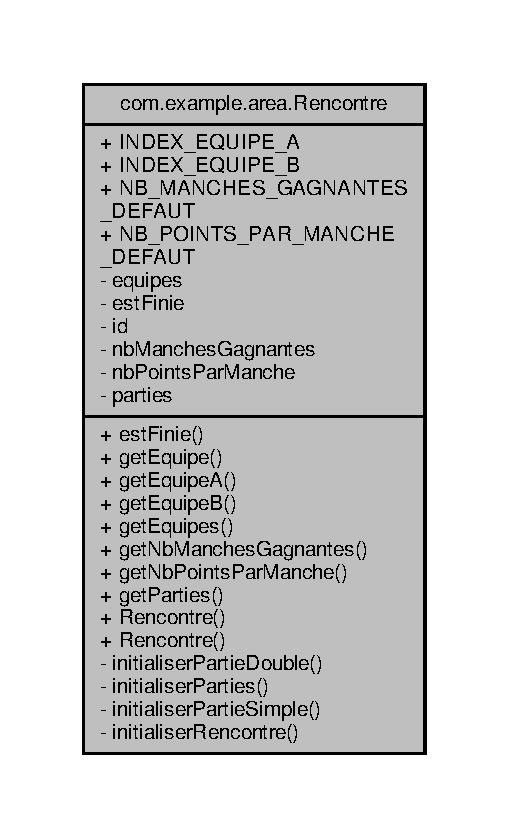
\includegraphics[width=244pt]{classcom_1_1example_1_1area_1_1_rencontre__coll__graph}
\end{center}
\end{figure}
\subsubsection*{Fonctions membres publiques}
\begin{DoxyCompactItemize}
\item 
boolean \hyperlink{classcom_1_1example_1_1area_1_1_rencontre_abafd9770f1e749026b7a4196648fa366}{est\+Finie} ()
\begin{DoxyCompactList}\small\item\em Accesseur de l\textquotesingle{}attribut est\+Finie. \end{DoxyCompactList}\item 
\hyperlink{classcom_1_1example_1_1area_1_1_equipe}{Equipe} \hyperlink{classcom_1_1example_1_1area_1_1_rencontre_a5bd76838a3c61a6e8e6204981218e10e}{get\+Equipe} (int index\+Equipe)
\begin{DoxyCompactList}\small\item\em Retourne l\textquotesingle{}objet \hyperlink{classcom_1_1example_1_1area_1_1_equipe}{Equipe} demandé \end{DoxyCompactList}\item 
\hyperlink{classcom_1_1example_1_1area_1_1_equipe}{Equipe} \hyperlink{classcom_1_1example_1_1area_1_1_rencontre_a207498fd691285b28b0a720da0a660f8}{get\+EquipeA} ()
\begin{DoxyCompactList}\small\item\em Accesseur de l\textquotesingle{}attribut equipeA. \end{DoxyCompactList}\item 
\hyperlink{classcom_1_1example_1_1area_1_1_equipe}{Equipe} \hyperlink{classcom_1_1example_1_1area_1_1_rencontre_a83deec026e26407049c5671672291170}{get\+EquipeB} ()
\begin{DoxyCompactList}\small\item\em Accesseur de l\textquotesingle{}attribut equipeB. \end{DoxyCompactList}\item 
Vector$<$ \hyperlink{classcom_1_1example_1_1area_1_1_equipe}{Equipe} $>$ \hyperlink{classcom_1_1example_1_1area_1_1_rencontre_a59f379be02ce6c587ad59d1b30e3c9a5}{get\+Equipes} ()
\begin{DoxyCompactList}\small\item\em Accesseur de l\textquotesingle{}attribut equipes. \end{DoxyCompactList}\item 
int \hyperlink{classcom_1_1example_1_1area_1_1_rencontre_a8f7801a28279d1fb26b0961d05c55bdd}{get\+Nb\+Manches\+Gagnantes} ()
\begin{DoxyCompactList}\small\item\em Accesseur de l\textquotesingle{}attribut nb\+Manches\+Gagnantes. \end{DoxyCompactList}\item 
int \hyperlink{classcom_1_1example_1_1area_1_1_rencontre_a539e26b8c59998880fcf9b7c9f2b685a}{get\+Nb\+Points\+Par\+Manche} ()
\begin{DoxyCompactList}\small\item\em Accesseur de l\textquotesingle{}attribut nb\+Points\+Par\+Manche. \end{DoxyCompactList}\item 
Vector$<$ \hyperlink{classcom_1_1example_1_1area_1_1_partie}{Partie} $>$ \hyperlink{classcom_1_1example_1_1area_1_1_rencontre_a58b62bd2f8a63f532df2bc8607268a2d}{get\+Parties} ()
\begin{DoxyCompactList}\small\item\em Accesseur de l\textquotesingle{}attribut parties. \end{DoxyCompactList}\item 
\hyperlink{classcom_1_1example_1_1area_1_1_rencontre_abc915d4578268471bfab8214928bbd74}{Rencontre} (\hyperlink{classcom_1_1example_1_1area_1_1_equipe}{Equipe} equipeA, \hyperlink{classcom_1_1example_1_1area_1_1_equipe}{Equipe} equipeB)
\begin{DoxyCompactList}\small\item\em Constructeur pour une rencontre avec les paramètres de partie par défaut. \end{DoxyCompactList}\item 
\hyperlink{classcom_1_1example_1_1area_1_1_rencontre_a28c1f3173d0d0a81abb80fac81a184d4}{Rencontre} (\hyperlink{classcom_1_1example_1_1area_1_1_equipe}{Equipe} equipeA, \hyperlink{classcom_1_1example_1_1area_1_1_equipe}{Equipe} equipeB, int \hyperlink{classcom_1_1example_1_1area_1_1_rencontre_aef266bd256aecd70fbd02cf07625ed14}{nb\+Manches\+Gagnantes}, int \hyperlink{classcom_1_1example_1_1area_1_1_rencontre_ae1849c4bcdcfbb2d336b750a36be1162}{nb\+Points\+Par\+Manche})
\begin{DoxyCompactList}\small\item\em Constructeur. \end{DoxyCompactList}\end{DoxyCompactItemize}
\subsubsection*{Attributs publics statiques}
\begin{DoxyCompactItemize}
\item 
static final int \hyperlink{classcom_1_1example_1_1area_1_1_rencontre_a673930c3156037739c3fa2aa335033d7}{I\+N\+D\+E\+X\+\_\+\+E\+Q\+U\+I\+P\+E\+\_\+A} = 0
\item 
static final int \hyperlink{classcom_1_1example_1_1area_1_1_rencontre_a08ed5cef8f2bbb80b2010bdb60c515d6}{I\+N\+D\+E\+X\+\_\+\+E\+Q\+U\+I\+P\+E\+\_\+B} = 1
\item 
static final int \hyperlink{classcom_1_1example_1_1area_1_1_rencontre_a9ab6dcd72bcb2ca3c21ed3fcba4a9b46}{N\+B\+\_\+\+M\+A\+N\+C\+H\+E\+S\+\_\+\+G\+A\+G\+N\+A\+N\+T\+E\+S\+\_\+\+D\+E\+F\+A\+UT} = 3
\begin{DoxyCompactList}\small\item\em nombre de manches (ou sets) par défaut pour remporter une \hyperlink{classcom_1_1example_1_1area_1_1_partie}{Partie} \end{DoxyCompactList}\item 
static final int \hyperlink{classcom_1_1example_1_1area_1_1_rencontre_ac2217d1cf2cf9310966619ba69214259}{N\+B\+\_\+\+P\+O\+I\+N\+T\+S\+\_\+\+P\+A\+R\+\_\+\+M\+A\+N\+C\+H\+E\+\_\+\+D\+E\+F\+A\+UT} = 11
\begin{DoxyCompactList}\small\item\em nombre de points par défaut pour remporter une manche (ou set) \end{DoxyCompactList}\end{DoxyCompactItemize}
\subsubsection*{Fonctions membres privées}
\begin{DoxyCompactItemize}
\item 
void \hyperlink{classcom_1_1example_1_1area_1_1_rencontre_a5dd70b0d58f74626bdb4bd21a21d661c}{initialiser\+Partie\+Double} (int index\+JoueurA, int index\+Deuxieme\+JoueurA, int index\+JoueurB, int index\+Deuxieme\+JoueurB)
\begin{DoxyCompactList}\small\item\em Initialise une partie en double. \end{DoxyCompactList}\item 
void \hyperlink{classcom_1_1example_1_1area_1_1_rencontre_a9af98788b76483567c06eac9a02418c5}{initialiser\+Parties} ()
\begin{DoxyCompactList}\small\item\em Initialise les parties selon l\textquotesingle{}ordre d\textquotesingle{}un feuille de rencontre. \end{DoxyCompactList}\item 
void \hyperlink{classcom_1_1example_1_1area_1_1_rencontre_afe8119a55e348caf296514d604718646}{initialiser\+Partie\+Simple} (int index\+JoueurA, int index\+JoueurB)
\begin{DoxyCompactList}\small\item\em Initialise une partie en simple. \end{DoxyCompactList}\item 
void \hyperlink{classcom_1_1example_1_1area_1_1_rencontre_a61ff55a4fb128654aec0456d5b3adaa3}{initialiser\+Rencontre} (\hyperlink{classcom_1_1example_1_1area_1_1_equipe}{Equipe} equipeA, \hyperlink{classcom_1_1example_1_1area_1_1_equipe}{Equipe} equipeB)
\begin{DoxyCompactList}\small\item\em Initialise une rencontre entre deux équipes. \end{DoxyCompactList}\end{DoxyCompactItemize}
\subsubsection*{Attributs privés}
\begin{DoxyCompactItemize}
\item 
Vector$<$ \hyperlink{classcom_1_1example_1_1area_1_1_equipe}{Equipe} $>$ \hyperlink{classcom_1_1example_1_1area_1_1_rencontre_accbafe5a878f457fb7119cfd55401c86}{equipes}
\begin{DoxyCompactList}\small\item\em les deux équipes \end{DoxyCompactList}\item 
boolean \hyperlink{classcom_1_1example_1_1area_1_1_rencontre_a2124164efb96db89312021ed57d795c1}{est\+Finie} = false
\begin{DoxyCompactList}\small\item\em l\textquotesingle{}état de la rencontre \end{DoxyCompactList}\item 
int \hyperlink{classcom_1_1example_1_1area_1_1_rencontre_a570f0dcf549626a6a87ab9e994279fde}{id} = 0
\begin{DoxyCompactList}\small\item\em l\textquotesingle{}identifiant de la rencontre \end{DoxyCompactList}\item 
int \hyperlink{classcom_1_1example_1_1area_1_1_rencontre_aef266bd256aecd70fbd02cf07625ed14}{nb\+Manches\+Gagnantes}
\begin{DoxyCompactList}\small\item\em nombre de manches (ou sets) pour remporter une \hyperlink{classcom_1_1example_1_1area_1_1_partie}{Partie} \end{DoxyCompactList}\item 
int \hyperlink{classcom_1_1example_1_1area_1_1_rencontre_ae1849c4bcdcfbb2d336b750a36be1162}{nb\+Points\+Par\+Manche}
\begin{DoxyCompactList}\small\item\em nombre de points pour remporter une manche (ou set) \end{DoxyCompactList}\item 
Vector$<$ \hyperlink{classcom_1_1example_1_1area_1_1_partie}{Partie} $>$ \hyperlink{classcom_1_1example_1_1area_1_1_rencontre_a9bdc6df389184fc2ecb4d87a7879213a}{parties}
\begin{DoxyCompactList}\small\item\em les parties d\textquotesingle{}une rencontre \end{DoxyCompactList}\end{DoxyCompactItemize}


\subsubsection{Description détaillée}
Classe qui permet la gestion d\textquotesingle{}une rencontre entre deux équipes. 

Définition à la ligne \hyperlink{_rencontre_8java_source_l00017}{17} du fichier \hyperlink{_rencontre_8java_source}{Rencontre.\+java}.



\subsubsection{Documentation des constructeurs et destructeur}
\mbox{\Hypertarget{classcom_1_1example_1_1area_1_1_rencontre_abc915d4578268471bfab8214928bbd74}\label{classcom_1_1example_1_1area_1_1_rencontre_abc915d4578268471bfab8214928bbd74}} 
\index{com\+::example\+::area\+::\+Rencontre@{com\+::example\+::area\+::\+Rencontre}!Rencontre@{Rencontre}}
\index{Rencontre@{Rencontre}!com\+::example\+::area\+::\+Rencontre@{com\+::example\+::area\+::\+Rencontre}}
\paragraph{\texorpdfstring{Rencontre()}{Rencontre()}\hspace{0.1cm}{\footnotesize\ttfamily [1/2]}}
{\footnotesize\ttfamily com.\+example.\+area.\+Rencontre.\+Rencontre (\begin{DoxyParamCaption}\item[{\hyperlink{classcom_1_1example_1_1area_1_1_equipe}{Equipe}}]{equipeA,  }\item[{\hyperlink{classcom_1_1example_1_1area_1_1_equipe}{Equipe}}]{equipeB }\end{DoxyParamCaption})}



Constructeur pour une rencontre avec les paramètres de partie par défaut. 


\begin{DoxyParams}{Paramètres}
{\em equipeA} & \\
\hline
{\em equipeB} & \\
\hline
\end{DoxyParams}


Définition à la ligne \hyperlink{_rencontre_8java_source_l00041}{41} du fichier \hyperlink{_rencontre_8java_source}{Rencontre.\+java}.



Références \hyperlink{_rencontre_8java_source_l00081}{com.\+example.\+area.\+Rencontre.\+initialiser\+Parties()}, \hyperlink{_rencontre_8java_source_l00071}{com.\+example.\+area.\+Rencontre.\+initialiser\+Rencontre()}, \hyperlink{_rencontre_8java_source_l00033}{com.\+example.\+area.\+Rencontre.\+N\+B\+\_\+\+M\+A\+N\+C\+H\+E\+S\+\_\+\+G\+A\+G\+N\+A\+N\+T\+E\+S\+\_\+\+D\+E\+F\+A\+UT}, et \hyperlink{_rencontre_8java_source_l00034}{com.\+example.\+area.\+Rencontre.\+N\+B\+\_\+\+P\+O\+I\+N\+T\+S\+\_\+\+P\+A\+R\+\_\+\+M\+A\+N\+C\+H\+E\+\_\+\+D\+E\+F\+A\+UT}.


\begin{DoxyCode}
00042     \{
00043         this.\hyperlink{classcom_1_1example_1_1area_1_1_rencontre_aef266bd256aecd70fbd02cf07625ed14}{nbManchesGagnantes} = \hyperlink{classcom_1_1example_1_1area_1_1_rencontre_a9ab6dcd72bcb2ca3c21ed3fcba4a9b46}{NB\_MANCHES\_GAGNANTES\_DEFAUT};
00044         this.\hyperlink{classcom_1_1example_1_1area_1_1_rencontre_ae1849c4bcdcfbb2d336b750a36be1162}{nbPointsParManche} = \hyperlink{classcom_1_1example_1_1area_1_1_rencontre_ac2217d1cf2cf9310966619ba69214259}{NB\_POINTS\_PAR\_MANCHE\_DEFAUT};
00045 
00046         \hyperlink{classcom_1_1example_1_1area_1_1_rencontre_a61ff55a4fb128654aec0456d5b3adaa3}{initialiserRencontre}(equipeA, equipeB);
00047 
00048         \hyperlink{classcom_1_1example_1_1area_1_1_rencontre_a9af98788b76483567c06eac9a02418c5}{initialiserParties}();
00049     \}
\end{DoxyCode}
\mbox{\Hypertarget{classcom_1_1example_1_1area_1_1_rencontre_a28c1f3173d0d0a81abb80fac81a184d4}\label{classcom_1_1example_1_1area_1_1_rencontre_a28c1f3173d0d0a81abb80fac81a184d4}} 
\index{com\+::example\+::area\+::\+Rencontre@{com\+::example\+::area\+::\+Rencontre}!Rencontre@{Rencontre}}
\index{Rencontre@{Rencontre}!com\+::example\+::area\+::\+Rencontre@{com\+::example\+::area\+::\+Rencontre}}
\paragraph{\texorpdfstring{Rencontre()}{Rencontre()}\hspace{0.1cm}{\footnotesize\ttfamily [2/2]}}
{\footnotesize\ttfamily com.\+example.\+area.\+Rencontre.\+Rencontre (\begin{DoxyParamCaption}\item[{\hyperlink{classcom_1_1example_1_1area_1_1_equipe}{Equipe}}]{equipeA,  }\item[{\hyperlink{classcom_1_1example_1_1area_1_1_equipe}{Equipe}}]{equipeB,  }\item[{int}]{nb\+Manches\+Gagnantes,  }\item[{int}]{nb\+Points\+Par\+Manche }\end{DoxyParamCaption})}



Constructeur. 


\begin{DoxyParams}{Paramètres}
{\em equipeA} & \\
\hline
{\em equipeB} & \\
\hline
{\em nb\+Manches\+Gagnantes} & nombre de manches (ou sets) pour remporter une \hyperlink{classcom_1_1example_1_1area_1_1_partie}{Partie} \\
\hline
{\em nb\+Points\+Par\+Manche} & nombre de points pour remporter une manche (ou set) \\
\hline
\end{DoxyParams}


Définition à la ligne \hyperlink{_rencontre_8java_source_l00058}{58} du fichier \hyperlink{_rencontre_8java_source}{Rencontre.\+java}.



Références \hyperlink{_rencontre_8java_source_l00081}{com.\+example.\+area.\+Rencontre.\+initialiser\+Parties()}, \hyperlink{_rencontre_8java_source_l00071}{com.\+example.\+area.\+Rencontre.\+initialiser\+Rencontre()}, \hyperlink{_rencontre_8java_source_l00026}{com.\+example.\+area.\+Rencontre.\+nb\+Manches\+Gagnantes}, et \hyperlink{_rencontre_8java_source_l00027}{com.\+example.\+area.\+Rencontre.\+nb\+Points\+Par\+Manche}.


\begin{DoxyCode}
00059     \{
00060         this.\hyperlink{classcom_1_1example_1_1area_1_1_rencontre_aef266bd256aecd70fbd02cf07625ed14}{nbManchesGagnantes} = \hyperlink{classcom_1_1example_1_1area_1_1_rencontre_aef266bd256aecd70fbd02cf07625ed14}{nbManchesGagnantes};
00061         this.\hyperlink{classcom_1_1example_1_1area_1_1_rencontre_ae1849c4bcdcfbb2d336b750a36be1162}{nbPointsParManche} = \hyperlink{classcom_1_1example_1_1area_1_1_rencontre_ae1849c4bcdcfbb2d336b750a36be1162}{nbPointsParManche};
00062 
00063         \hyperlink{classcom_1_1example_1_1area_1_1_rencontre_a61ff55a4fb128654aec0456d5b3adaa3}{initialiserRencontre}(equipeA, equipeB);
00064 
00065         \hyperlink{classcom_1_1example_1_1area_1_1_rencontre_a9af98788b76483567c06eac9a02418c5}{initialiserParties}();
00066     \}
\end{DoxyCode}


\subsubsection{Documentation des fonctions membres}
\mbox{\Hypertarget{classcom_1_1example_1_1area_1_1_rencontre_abafd9770f1e749026b7a4196648fa366}\label{classcom_1_1example_1_1area_1_1_rencontre_abafd9770f1e749026b7a4196648fa366}} 
\index{com\+::example\+::area\+::\+Rencontre@{com\+::example\+::area\+::\+Rencontre}!est\+Finie@{est\+Finie}}
\index{est\+Finie@{est\+Finie}!com\+::example\+::area\+::\+Rencontre@{com\+::example\+::area\+::\+Rencontre}}
\paragraph{\texorpdfstring{est\+Finie()}{estFinie()}}
{\footnotesize\ttfamily boolean com.\+example.\+area.\+Rencontre.\+est\+Finie (\begin{DoxyParamCaption}{ }\end{DoxyParamCaption})}



Accesseur de l\textquotesingle{}attribut est\+Finie. 

\begin{DoxyReturn}{Renvoie}
boolean 
\end{DoxyReturn}


Définition à la ligne \hyperlink{_rencontre_8java_source_l00195}{195} du fichier \hyperlink{_rencontre_8java_source}{Rencontre.\+java}.


\begin{DoxyCode}
00196     \{
00197         \textcolor{keywordflow}{return} this.\hyperlink{classcom_1_1example_1_1area_1_1_rencontre_abafd9770f1e749026b7a4196648fa366}{estFinie};
00198     \}
\end{DoxyCode}
\mbox{\Hypertarget{classcom_1_1example_1_1area_1_1_rencontre_a5bd76838a3c61a6e8e6204981218e10e}\label{classcom_1_1example_1_1area_1_1_rencontre_a5bd76838a3c61a6e8e6204981218e10e}} 
\index{com\+::example\+::area\+::\+Rencontre@{com\+::example\+::area\+::\+Rencontre}!get\+Equipe@{get\+Equipe}}
\index{get\+Equipe@{get\+Equipe}!com\+::example\+::area\+::\+Rencontre@{com\+::example\+::area\+::\+Rencontre}}
\paragraph{\texorpdfstring{get\+Equipe()}{getEquipe()}}
{\footnotesize\ttfamily \hyperlink{classcom_1_1example_1_1area_1_1_equipe}{Equipe} com.\+example.\+area.\+Rencontre.\+get\+Equipe (\begin{DoxyParamCaption}\item[{int}]{index\+Equipe }\end{DoxyParamCaption})}



Retourne l\textquotesingle{}objet \hyperlink{classcom_1_1example_1_1area_1_1_equipe}{Equipe} demandé 


\begin{DoxyParams}{Paramètres}
{\em index\+Equipe} & l\textquotesingle{}index de l\textquotesingle{}équipe à retourner \\
\hline
\end{DoxyParams}
\begin{DoxyReturn}{Renvoie}
\hyperlink{classcom_1_1example_1_1area_1_1_equipe}{Equipe} l\textquotesingle{}équipe A ou B 
\end{DoxyReturn}


Définition à la ligne \hyperlink{_rencontre_8java_source_l00168}{168} du fichier \hyperlink{_rencontre_8java_source}{Rencontre.\+java}.


\begin{DoxyCode}
00169     \{
00170         \textcolor{keywordflow}{return} this.\hyperlink{classcom_1_1example_1_1area_1_1_rencontre_accbafe5a878f457fb7119cfd55401c86}{equipes}.get(indexEquipe);
00171     \}
\end{DoxyCode}
\mbox{\Hypertarget{classcom_1_1example_1_1area_1_1_rencontre_a207498fd691285b28b0a720da0a660f8}\label{classcom_1_1example_1_1area_1_1_rencontre_a207498fd691285b28b0a720da0a660f8}} 
\index{com\+::example\+::area\+::\+Rencontre@{com\+::example\+::area\+::\+Rencontre}!get\+EquipeA@{get\+EquipeA}}
\index{get\+EquipeA@{get\+EquipeA}!com\+::example\+::area\+::\+Rencontre@{com\+::example\+::area\+::\+Rencontre}}
\paragraph{\texorpdfstring{get\+Equipe\+A()}{getEquipeA()}}
{\footnotesize\ttfamily \hyperlink{classcom_1_1example_1_1area_1_1_equipe}{Equipe} com.\+example.\+area.\+Rencontre.\+get\+EquipeA (\begin{DoxyParamCaption}{ }\end{DoxyParamCaption})}



Accesseur de l\textquotesingle{}attribut equipeA. 

\begin{DoxyReturn}{Renvoie}
\hyperlink{classcom_1_1example_1_1area_1_1_equipe}{Equipe} l\textquotesingle{}équipe A 
\end{DoxyReturn}


Définition à la ligne \hyperlink{_rencontre_8java_source_l00177}{177} du fichier \hyperlink{_rencontre_8java_source}{Rencontre.\+java}.



Référencé par \hyperlink{_i_h_m_gestion_rencontre_8java_source_l00142}{com.\+example.\+area.\+I\+H\+M\+Gestion\+Rencontre.\+initialiser\+Ressources\+I\+H\+M()}, et \hyperlink{_i_h_m_gestion_rencontre_8java_source_l00281}{com.\+example.\+area.\+I\+H\+M\+Gestion\+Rencontre.\+recuperer\+Noms\+Joueurs()}.


\begin{DoxyCode}
00178     \{
00179         \textcolor{keywordflow}{return} this.\hyperlink{classcom_1_1example_1_1area_1_1_rencontre_accbafe5a878f457fb7119cfd55401c86}{equipes}.get(\hyperlink{classcom_1_1example_1_1area_1_1_rencontre_a673930c3156037739c3fa2aa335033d7}{INDEX\_EQUIPE\_A});
00180     \}
\end{DoxyCode}
\mbox{\Hypertarget{classcom_1_1example_1_1area_1_1_rencontre_a83deec026e26407049c5671672291170}\label{classcom_1_1example_1_1area_1_1_rencontre_a83deec026e26407049c5671672291170}} 
\index{com\+::example\+::area\+::\+Rencontre@{com\+::example\+::area\+::\+Rencontre}!get\+EquipeB@{get\+EquipeB}}
\index{get\+EquipeB@{get\+EquipeB}!com\+::example\+::area\+::\+Rencontre@{com\+::example\+::area\+::\+Rencontre}}
\paragraph{\texorpdfstring{get\+Equipe\+B()}{getEquipeB()}}
{\footnotesize\ttfamily \hyperlink{classcom_1_1example_1_1area_1_1_equipe}{Equipe} com.\+example.\+area.\+Rencontre.\+get\+EquipeB (\begin{DoxyParamCaption}{ }\end{DoxyParamCaption})}



Accesseur de l\textquotesingle{}attribut equipeB. 

\begin{DoxyReturn}{Renvoie}
\hyperlink{classcom_1_1example_1_1area_1_1_equipe}{Equipe} l\textquotesingle{}équipe B 
\end{DoxyReturn}


Définition à la ligne \hyperlink{_rencontre_8java_source_l00186}{186} du fichier \hyperlink{_rencontre_8java_source}{Rencontre.\+java}.



Référencé par \hyperlink{_i_h_m_gestion_rencontre_8java_source_l00142}{com.\+example.\+area.\+I\+H\+M\+Gestion\+Rencontre.\+initialiser\+Ressources\+I\+H\+M()}, et \hyperlink{_i_h_m_gestion_rencontre_8java_source_l00281}{com.\+example.\+area.\+I\+H\+M\+Gestion\+Rencontre.\+recuperer\+Noms\+Joueurs()}.


\begin{DoxyCode}
00187     \{
00188         \textcolor{keywordflow}{return} this.\hyperlink{classcom_1_1example_1_1area_1_1_rencontre_accbafe5a878f457fb7119cfd55401c86}{equipes}.get(\hyperlink{classcom_1_1example_1_1area_1_1_rencontre_a08ed5cef8f2bbb80b2010bdb60c515d6}{INDEX\_EQUIPE\_B});
00189     \}
\end{DoxyCode}
\mbox{\Hypertarget{classcom_1_1example_1_1area_1_1_rencontre_a59f379be02ce6c587ad59d1b30e3c9a5}\label{classcom_1_1example_1_1area_1_1_rencontre_a59f379be02ce6c587ad59d1b30e3c9a5}} 
\index{com\+::example\+::area\+::\+Rencontre@{com\+::example\+::area\+::\+Rencontre}!get\+Equipes@{get\+Equipes}}
\index{get\+Equipes@{get\+Equipes}!com\+::example\+::area\+::\+Rencontre@{com\+::example\+::area\+::\+Rencontre}}
\paragraph{\texorpdfstring{get\+Equipes()}{getEquipes()}}
{\footnotesize\ttfamily Vector$<$\hyperlink{classcom_1_1example_1_1area_1_1_equipe}{Equipe}$>$ com.\+example.\+area.\+Rencontre.\+get\+Equipes (\begin{DoxyParamCaption}{ }\end{DoxyParamCaption})}



Accesseur de l\textquotesingle{}attribut equipes. 

\begin{DoxyReturn}{Renvoie}
Vector$<$\+Equipe$>$ les deux objets \hyperlink{classcom_1_1example_1_1area_1_1_equipe}{Equipe} 
\end{DoxyReturn}


Définition à la ligne \hyperlink{_rencontre_8java_source_l00149}{149} du fichier \hyperlink{_rencontre_8java_source}{Rencontre.\+java}.



Références \hyperlink{_rencontre_8java_source_l00022}{com.\+example.\+area.\+Rencontre.\+equipes}.


\begin{DoxyCode}
00150     \{
00151         \textcolor{keywordflow}{return} this.\hyperlink{classcom_1_1example_1_1area_1_1_rencontre_accbafe5a878f457fb7119cfd55401c86}{equipes};
00152     \}
\end{DoxyCode}
\mbox{\Hypertarget{classcom_1_1example_1_1area_1_1_rencontre_a8f7801a28279d1fb26b0961d05c55bdd}\label{classcom_1_1example_1_1area_1_1_rencontre_a8f7801a28279d1fb26b0961d05c55bdd}} 
\index{com\+::example\+::area\+::\+Rencontre@{com\+::example\+::area\+::\+Rencontre}!get\+Nb\+Manches\+Gagnantes@{get\+Nb\+Manches\+Gagnantes}}
\index{get\+Nb\+Manches\+Gagnantes@{get\+Nb\+Manches\+Gagnantes}!com\+::example\+::area\+::\+Rencontre@{com\+::example\+::area\+::\+Rencontre}}
\paragraph{\texorpdfstring{get\+Nb\+Manches\+Gagnantes()}{getNbManchesGagnantes()}}
{\footnotesize\ttfamily int com.\+example.\+area.\+Rencontre.\+get\+Nb\+Manches\+Gagnantes (\begin{DoxyParamCaption}{ }\end{DoxyParamCaption})}



Accesseur de l\textquotesingle{}attribut nb\+Manches\+Gagnantes. 

\begin{DoxyReturn}{Renvoie}
int 
\end{DoxyReturn}


Définition à la ligne \hyperlink{_rencontre_8java_source_l00204}{204} du fichier \hyperlink{_rencontre_8java_source}{Rencontre.\+java}.



Références \hyperlink{_rencontre_8java_source_l00026}{com.\+example.\+area.\+Rencontre.\+nb\+Manches\+Gagnantes}.


\begin{DoxyCode}
00205     \{
00206         \textcolor{keywordflow}{return} this.\hyperlink{classcom_1_1example_1_1area_1_1_rencontre_aef266bd256aecd70fbd02cf07625ed14}{nbManchesGagnantes};
00207     \}
\end{DoxyCode}
\mbox{\Hypertarget{classcom_1_1example_1_1area_1_1_rencontre_a539e26b8c59998880fcf9b7c9f2b685a}\label{classcom_1_1example_1_1area_1_1_rencontre_a539e26b8c59998880fcf9b7c9f2b685a}} 
\index{com\+::example\+::area\+::\+Rencontre@{com\+::example\+::area\+::\+Rencontre}!get\+Nb\+Points\+Par\+Manche@{get\+Nb\+Points\+Par\+Manche}}
\index{get\+Nb\+Points\+Par\+Manche@{get\+Nb\+Points\+Par\+Manche}!com\+::example\+::area\+::\+Rencontre@{com\+::example\+::area\+::\+Rencontre}}
\paragraph{\texorpdfstring{get\+Nb\+Points\+Par\+Manche()}{getNbPointsParManche()}}
{\footnotesize\ttfamily int com.\+example.\+area.\+Rencontre.\+get\+Nb\+Points\+Par\+Manche (\begin{DoxyParamCaption}{ }\end{DoxyParamCaption})}



Accesseur de l\textquotesingle{}attribut nb\+Points\+Par\+Manche. 

\begin{DoxyReturn}{Renvoie}
int 
\end{DoxyReturn}


Définition à la ligne \hyperlink{_rencontre_8java_source_l00213}{213} du fichier \hyperlink{_rencontre_8java_source}{Rencontre.\+java}.



Références \hyperlink{_rencontre_8java_source_l00027}{com.\+example.\+area.\+Rencontre.\+nb\+Points\+Par\+Manche}.


\begin{DoxyCode}
00214     \{
00215         \textcolor{keywordflow}{return} this.\hyperlink{classcom_1_1example_1_1area_1_1_rencontre_ae1849c4bcdcfbb2d336b750a36be1162}{nbPointsParManche};
00216     \}
\end{DoxyCode}
\mbox{\Hypertarget{classcom_1_1example_1_1area_1_1_rencontre_a58b62bd2f8a63f532df2bc8607268a2d}\label{classcom_1_1example_1_1area_1_1_rencontre_a58b62bd2f8a63f532df2bc8607268a2d}} 
\index{com\+::example\+::area\+::\+Rencontre@{com\+::example\+::area\+::\+Rencontre}!get\+Parties@{get\+Parties}}
\index{get\+Parties@{get\+Parties}!com\+::example\+::area\+::\+Rencontre@{com\+::example\+::area\+::\+Rencontre}}
\paragraph{\texorpdfstring{get\+Parties()}{getParties()}}
{\footnotesize\ttfamily Vector$<$\hyperlink{classcom_1_1example_1_1area_1_1_partie}{Partie}$>$ com.\+example.\+area.\+Rencontre.\+get\+Parties (\begin{DoxyParamCaption}{ }\end{DoxyParamCaption})}



Accesseur de l\textquotesingle{}attribut parties. 

\begin{DoxyReturn}{Renvoie}
Vector$<$\+Partie$>$ les parties de la rencontre 
\end{DoxyReturn}


Définition à la ligne \hyperlink{_rencontre_8java_source_l00158}{158} du fichier \hyperlink{_rencontre_8java_source}{Rencontre.\+java}.



Références \hyperlink{_rencontre_8java_source_l00023}{com.\+example.\+area.\+Rencontre.\+parties}.



Référencé par \hyperlink{_i_h_m_gestion_rencontre_8java_source_l00322}{com.\+example.\+area.\+I\+H\+M\+Gestion\+Rencontre.\+afficher\+Parties()}, et \hyperlink{_i_h_m_gestion_rencontre_8java_source_l00158}{com.\+example.\+area.\+I\+H\+M\+Gestion\+Rencontre.\+connecter\+Boutons()}.


\begin{DoxyCode}
00159     \{
00160         \textcolor{keywordflow}{return} \hyperlink{classcom_1_1example_1_1area_1_1_rencontre_a9bdc6df389184fc2ecb4d87a7879213a}{parties};
00161     \}
\end{DoxyCode}
\mbox{\Hypertarget{classcom_1_1example_1_1area_1_1_rencontre_a5dd70b0d58f74626bdb4bd21a21d661c}\label{classcom_1_1example_1_1area_1_1_rencontre_a5dd70b0d58f74626bdb4bd21a21d661c}} 
\index{com\+::example\+::area\+::\+Rencontre@{com\+::example\+::area\+::\+Rencontre}!initialiser\+Partie\+Double@{initialiser\+Partie\+Double}}
\index{initialiser\+Partie\+Double@{initialiser\+Partie\+Double}!com\+::example\+::area\+::\+Rencontre@{com\+::example\+::area\+::\+Rencontre}}
\paragraph{\texorpdfstring{initialiser\+Partie\+Double()}{initialiserPartieDouble()}}
{\footnotesize\ttfamily void com.\+example.\+area.\+Rencontre.\+initialiser\+Partie\+Double (\begin{DoxyParamCaption}\item[{int}]{index\+JoueurA,  }\item[{int}]{index\+Deuxieme\+JoueurA,  }\item[{int}]{index\+JoueurB,  }\item[{int}]{index\+Deuxieme\+JoueurB }\end{DoxyParamCaption})\hspace{0.3cm}{\ttfamily [private]}}



Initialise une partie en double. 


\begin{DoxyParams}{Paramètres}
{\em index\+JoueurA} & l\textquotesingle{}index du joueur dans l\textquotesingle{}équipe A \\
\hline
{\em index\+Deuxieme\+JoueurA} & l\textquotesingle{}index du deuxième joueur dans l\textquotesingle{}équipe A \\
\hline
{\em index\+JoueurB} & l\textquotesingle{}index du joueur dans l\textquotesingle{}équipe B \\
\hline
{\em index\+Deuxieme\+JoueurB} & l\textquotesingle{}index du deuxième joueur dans l\textquotesingle{}équipe B \\
\hline
\end{DoxyParams}


Définition à la ligne \hyperlink{_rencontre_8java_source_l00130}{130} du fichier \hyperlink{_rencontre_8java_source}{Rencontre.\+java}.



Référencé par \hyperlink{_rencontre_8java_source_l00081}{com.\+example.\+area.\+Rencontre.\+initialiser\+Parties()}.


\begin{DoxyCode}
00131     \{
00132       Vector<Joueur> joueursPartiesA = \textcolor{keyword}{new} Vector<Joueur>();
00133       Vector<Joueur> joueursPartiesB = \textcolor{keyword}{new} Vector<Joueur>();
00134 
00135       Vector<Joueur> joueursEquipeA = this.\hyperlink{classcom_1_1example_1_1area_1_1_rencontre_accbafe5a878f457fb7119cfd55401c86}{equipes}.get(\hyperlink{classcom_1_1example_1_1area_1_1_rencontre_a673930c3156037739c3fa2aa335033d7}{INDEX\_EQUIPE\_A}).getJoueurs();
00136       Vector<Joueur> joueursEquipeB = this.\hyperlink{classcom_1_1example_1_1area_1_1_rencontre_accbafe5a878f457fb7119cfd55401c86}{equipes}.get(\hyperlink{classcom_1_1example_1_1area_1_1_rencontre_a08ed5cef8f2bbb80b2010bdb60c515d6}{INDEX\_EQUIPE\_B}).getJoueurs();
00137 
00138       joueursPartiesA.add(joueursEquipeA.elementAt(indexJoueurA));
00139       joueursPartiesA.add(joueursEquipeA.elementAt(indexDeuxiemeJoueurA));
00140       joueursPartiesB.add(joueursEquipeB.elementAt(indexJoueurB));
00141       joueursPartiesB.add(joueursEquipeB.elementAt(indexDeuxiemeJoueurB));
00142       \hyperlink{classcom_1_1example_1_1area_1_1_rencontre_a9bdc6df389184fc2ecb4d87a7879213a}{parties}.add(\textcolor{keyword}{new} Partie(this.\hyperlink{classcom_1_1example_1_1area_1_1_rencontre_aef266bd256aecd70fbd02cf07625ed14}{nbManchesGagnantes}, this.
      \hyperlink{classcom_1_1example_1_1area_1_1_rencontre_ae1849c4bcdcfbb2d336b750a36be1162}{nbPointsParManche}, joueursPartiesA, joueursPartiesB));
00143     \}
\end{DoxyCode}
\mbox{\Hypertarget{classcom_1_1example_1_1area_1_1_rencontre_a9af98788b76483567c06eac9a02418c5}\label{classcom_1_1example_1_1area_1_1_rencontre_a9af98788b76483567c06eac9a02418c5}} 
\index{com\+::example\+::area\+::\+Rencontre@{com\+::example\+::area\+::\+Rencontre}!initialiser\+Parties@{initialiser\+Parties}}
\index{initialiser\+Parties@{initialiser\+Parties}!com\+::example\+::area\+::\+Rencontre@{com\+::example\+::area\+::\+Rencontre}}
\paragraph{\texorpdfstring{initialiser\+Parties()}{initialiserParties()}}
{\footnotesize\ttfamily void com.\+example.\+area.\+Rencontre.\+initialiser\+Parties (\begin{DoxyParamCaption}{ }\end{DoxyParamCaption})\hspace{0.3cm}{\ttfamily [private]}}



Initialise les parties selon l\textquotesingle{}ordre d\textquotesingle{}un feuille de rencontre. 



Définition à la ligne \hyperlink{_rencontre_8java_source_l00081}{81} du fichier \hyperlink{_rencontre_8java_source}{Rencontre.\+java}.



Références \hyperlink{_equipe_8java_source_l00015}{com.\+example.\+area.\+Equipe.\+I\+N\+D\+E\+X\+\_\+\+J\+O\+U\+E\+U\+R\+\_\+A}, \hyperlink{_equipe_8java_source_l00016}{com.\+example.\+area.\+Equipe.\+I\+N\+D\+E\+X\+\_\+\+J\+O\+U\+E\+U\+R\+\_\+B}, \hyperlink{_equipe_8java_source_l00017}{com.\+example.\+area.\+Equipe.\+I\+N\+D\+E\+X\+\_\+\+J\+O\+U\+E\+U\+R\+\_\+C}, \hyperlink{_equipe_8java_source_l00018}{com.\+example.\+area.\+Equipe.\+I\+N\+D\+E\+X\+\_\+\+J\+O\+U\+E\+U\+R\+\_\+D}, \hyperlink{_equipe_8java_source_l00020}{com.\+example.\+area.\+Equipe.\+I\+N\+D\+E\+X\+\_\+\+J\+O\+U\+E\+U\+R\+\_\+W}, \hyperlink{_equipe_8java_source_l00021}{com.\+example.\+area.\+Equipe.\+I\+N\+D\+E\+X\+\_\+\+J\+O\+U\+E\+U\+R\+\_\+X}, \hyperlink{_equipe_8java_source_l00022}{com.\+example.\+area.\+Equipe.\+I\+N\+D\+E\+X\+\_\+\+J\+O\+U\+E\+U\+R\+\_\+Y}, \hyperlink{_equipe_8java_source_l00023}{com.\+example.\+area.\+Equipe.\+I\+N\+D\+E\+X\+\_\+\+J\+O\+U\+E\+U\+R\+\_\+Z}, \hyperlink{_rencontre_8java_source_l00130}{com.\+example.\+area.\+Rencontre.\+initialiser\+Partie\+Double()}, et \hyperlink{_rencontre_8java_source_l00110}{com.\+example.\+area.\+Rencontre.\+initialiser\+Partie\+Simple()}.



Référencé par \hyperlink{_rencontre_8java_source_l00041}{com.\+example.\+area.\+Rencontre.\+Rencontre()}.


\begin{DoxyCode}
00082     \{
00083         this.\hyperlink{classcom_1_1example_1_1area_1_1_rencontre_a9bdc6df389184fc2ecb4d87a7879213a}{parties} = \textcolor{keyword}{new} Vector<Partie>();
00084 
00085         \hyperlink{classcom_1_1example_1_1area_1_1_rencontre_afe8119a55e348caf296514d604718646}{initialiserPartieSimple}(Equipe.INDEX\_JOUEUR\_A, Equipe.INDEX\_JOUEUR\_W);
00086         \hyperlink{classcom_1_1example_1_1area_1_1_rencontre_afe8119a55e348caf296514d604718646}{initialiserPartieSimple}(Equipe.INDEX\_JOUEUR\_B, Equipe.INDEX\_JOUEUR\_X);
00087         \hyperlink{classcom_1_1example_1_1area_1_1_rencontre_afe8119a55e348caf296514d604718646}{initialiserPartieSimple}(Equipe.INDEX\_JOUEUR\_C, Equipe.INDEX\_JOUEUR\_Y);
00088         \hyperlink{classcom_1_1example_1_1area_1_1_rencontre_afe8119a55e348caf296514d604718646}{initialiserPartieSimple}(Equipe.INDEX\_JOUEUR\_D, Equipe.INDEX\_JOUEUR\_Z);
00089         \hyperlink{classcom_1_1example_1_1area_1_1_rencontre_afe8119a55e348caf296514d604718646}{initialiserPartieSimple}(Equipe.INDEX\_JOUEUR\_A, Equipe.INDEX\_JOUEUR\_X);
00090         \hyperlink{classcom_1_1example_1_1area_1_1_rencontre_afe8119a55e348caf296514d604718646}{initialiserPartieSimple}(Equipe.INDEX\_JOUEUR\_B, Equipe.INDEX\_JOUEUR\_W);
00091         \hyperlink{classcom_1_1example_1_1area_1_1_rencontre_afe8119a55e348caf296514d604718646}{initialiserPartieSimple}(Equipe.INDEX\_JOUEUR\_D, Equipe.INDEX\_JOUEUR\_Y);
00092         \hyperlink{classcom_1_1example_1_1area_1_1_rencontre_afe8119a55e348caf296514d604718646}{initialiserPartieSimple}(Equipe.INDEX\_JOUEUR\_C, Equipe.INDEX\_JOUEUR\_Z);
00093         \hyperlink{classcom_1_1example_1_1area_1_1_rencontre_a5dd70b0d58f74626bdb4bd21a21d661c}{initialiserPartieDouble}(Equipe.INDEX\_JOUEUR\_A, Equipe.INDEX\_JOUEUR\_B, Equipe
      .INDEX\_JOUEUR\_W, Equipe.INDEX\_JOUEUR\_Y);
00094         \hyperlink{classcom_1_1example_1_1area_1_1_rencontre_a5dd70b0d58f74626bdb4bd21a21d661c}{initialiserPartieDouble}(Equipe.INDEX\_JOUEUR\_C, Equipe.INDEX\_JOUEUR\_D, Equipe
      .INDEX\_JOUEUR\_X, Equipe.INDEX\_JOUEUR\_Z);
00095         \hyperlink{classcom_1_1example_1_1area_1_1_rencontre_afe8119a55e348caf296514d604718646}{initialiserPartieSimple}(Equipe.INDEX\_JOUEUR\_D, Equipe.INDEX\_JOUEUR\_W);
00096         \hyperlink{classcom_1_1example_1_1area_1_1_rencontre_afe8119a55e348caf296514d604718646}{initialiserPartieSimple}(Equipe.INDEX\_JOUEUR\_C, Equipe.INDEX\_JOUEUR\_X);
00097         \hyperlink{classcom_1_1example_1_1area_1_1_rencontre_afe8119a55e348caf296514d604718646}{initialiserPartieSimple}(Equipe.INDEX\_JOUEUR\_A, Equipe.INDEX\_JOUEUR\_Z);
00098         \hyperlink{classcom_1_1example_1_1area_1_1_rencontre_afe8119a55e348caf296514d604718646}{initialiserPartieSimple}(Equipe.INDEX\_JOUEUR\_B, Equipe.INDEX\_JOUEUR\_Y);
00099         \hyperlink{classcom_1_1example_1_1area_1_1_rencontre_afe8119a55e348caf296514d604718646}{initialiserPartieSimple}(Equipe.INDEX\_JOUEUR\_C, Equipe.INDEX\_JOUEUR\_W);
00100         \hyperlink{classcom_1_1example_1_1area_1_1_rencontre_afe8119a55e348caf296514d604718646}{initialiserPartieSimple}(Equipe.INDEX\_JOUEUR\_D, Equipe.INDEX\_JOUEUR\_X);
00101         \hyperlink{classcom_1_1example_1_1area_1_1_rencontre_afe8119a55e348caf296514d604718646}{initialiserPartieSimple}(Equipe.INDEX\_JOUEUR\_A, Equipe.INDEX\_JOUEUR\_Y);
00102         \hyperlink{classcom_1_1example_1_1area_1_1_rencontre_afe8119a55e348caf296514d604718646}{initialiserPartieSimple}(Equipe.INDEX\_JOUEUR\_B, Equipe.INDEX\_JOUEUR\_Z);
00103     \}
\end{DoxyCode}
\mbox{\Hypertarget{classcom_1_1example_1_1area_1_1_rencontre_afe8119a55e348caf296514d604718646}\label{classcom_1_1example_1_1area_1_1_rencontre_afe8119a55e348caf296514d604718646}} 
\index{com\+::example\+::area\+::\+Rencontre@{com\+::example\+::area\+::\+Rencontre}!initialiser\+Partie\+Simple@{initialiser\+Partie\+Simple}}
\index{initialiser\+Partie\+Simple@{initialiser\+Partie\+Simple}!com\+::example\+::area\+::\+Rencontre@{com\+::example\+::area\+::\+Rencontre}}
\paragraph{\texorpdfstring{initialiser\+Partie\+Simple()}{initialiserPartieSimple()}}
{\footnotesize\ttfamily void com.\+example.\+area.\+Rencontre.\+initialiser\+Partie\+Simple (\begin{DoxyParamCaption}\item[{int}]{index\+JoueurA,  }\item[{int}]{index\+JoueurB }\end{DoxyParamCaption})\hspace{0.3cm}{\ttfamily [private]}}



Initialise une partie en simple. 


\begin{DoxyParams}{Paramètres}
{\em index\+JoueurA} & l\textquotesingle{}index du joueur dans l\textquotesingle{}équipe A \\
\hline
{\em index\+JoueurB} & l\textquotesingle{}index du joueur dans l\textquotesingle{}équipe B \\
\hline
\end{DoxyParams}


Définition à la ligne \hyperlink{_rencontre_8java_source_l00110}{110} du fichier \hyperlink{_rencontre_8java_source}{Rencontre.\+java}.



Référencé par \hyperlink{_rencontre_8java_source_l00081}{com.\+example.\+area.\+Rencontre.\+initialiser\+Parties()}.


\begin{DoxyCode}
00111     \{
00112         Vector<Joueur> joueursPartiesA = \textcolor{keyword}{new} Vector<Joueur>();
00113         Vector<Joueur> joueursPartiesB = \textcolor{keyword}{new} Vector<Joueur>();
00114 
00115         Vector<Joueur> joueursEquipeA = this.\hyperlink{classcom_1_1example_1_1area_1_1_rencontre_accbafe5a878f457fb7119cfd55401c86}{equipes}.get(\hyperlink{classcom_1_1example_1_1area_1_1_rencontre_a673930c3156037739c3fa2aa335033d7}{INDEX\_EQUIPE\_A}).getJoueurs();
00116         Vector<Joueur> joueursEquipeB = this.\hyperlink{classcom_1_1example_1_1area_1_1_rencontre_accbafe5a878f457fb7119cfd55401c86}{equipes}.get(\hyperlink{classcom_1_1example_1_1area_1_1_rencontre_a08ed5cef8f2bbb80b2010bdb60c515d6}{INDEX\_EQUIPE\_B}).getJoueurs();
00117 
00118         joueursPartiesA.add(joueursEquipeA.elementAt(indexJoueurA));
00119         joueursPartiesB.add(joueursEquipeB.elementAt(indexJoueurB));
00120         \hyperlink{classcom_1_1example_1_1area_1_1_rencontre_a9bdc6df389184fc2ecb4d87a7879213a}{parties}.add(\textcolor{keyword}{new} Partie(this.\hyperlink{classcom_1_1example_1_1area_1_1_rencontre_aef266bd256aecd70fbd02cf07625ed14}{nbManchesGagnantes}, this.
      \hyperlink{classcom_1_1example_1_1area_1_1_rencontre_ae1849c4bcdcfbb2d336b750a36be1162}{nbPointsParManche}, joueursPartiesA, joueursPartiesB));
00121     \}
\end{DoxyCode}
\mbox{\Hypertarget{classcom_1_1example_1_1area_1_1_rencontre_a61ff55a4fb128654aec0456d5b3adaa3}\label{classcom_1_1example_1_1area_1_1_rencontre_a61ff55a4fb128654aec0456d5b3adaa3}} 
\index{com\+::example\+::area\+::\+Rencontre@{com\+::example\+::area\+::\+Rencontre}!initialiser\+Rencontre@{initialiser\+Rencontre}}
\index{initialiser\+Rencontre@{initialiser\+Rencontre}!com\+::example\+::area\+::\+Rencontre@{com\+::example\+::area\+::\+Rencontre}}
\paragraph{\texorpdfstring{initialiser\+Rencontre()}{initialiserRencontre()}}
{\footnotesize\ttfamily void com.\+example.\+area.\+Rencontre.\+initialiser\+Rencontre (\begin{DoxyParamCaption}\item[{\hyperlink{classcom_1_1example_1_1area_1_1_equipe}{Equipe}}]{equipeA,  }\item[{\hyperlink{classcom_1_1example_1_1area_1_1_equipe}{Equipe}}]{equipeB }\end{DoxyParamCaption})\hspace{0.3cm}{\ttfamily [private]}}



Initialise une rencontre entre deux équipes. 



Définition à la ligne \hyperlink{_rencontre_8java_source_l00071}{71} du fichier \hyperlink{_rencontre_8java_source}{Rencontre.\+java}.



Référencé par \hyperlink{_rencontre_8java_source_l00041}{com.\+example.\+area.\+Rencontre.\+Rencontre()}.


\begin{DoxyCode}
00072     \{
00073         this.\hyperlink{classcom_1_1example_1_1area_1_1_rencontre_accbafe5a878f457fb7119cfd55401c86}{equipes} = \textcolor{keyword}{new} Vector<Equipe>();
00074         this.\hyperlink{classcom_1_1example_1_1area_1_1_rencontre_accbafe5a878f457fb7119cfd55401c86}{equipes}.add(equipeA);
00075         this.\hyperlink{classcom_1_1example_1_1area_1_1_rencontre_accbafe5a878f457fb7119cfd55401c86}{equipes}.add(equipeB);
00076     \}
\end{DoxyCode}


\subsubsection{Documentation des données membres}
\mbox{\Hypertarget{classcom_1_1example_1_1area_1_1_rencontre_accbafe5a878f457fb7119cfd55401c86}\label{classcom_1_1example_1_1area_1_1_rencontre_accbafe5a878f457fb7119cfd55401c86}} 
\index{com\+::example\+::area\+::\+Rencontre@{com\+::example\+::area\+::\+Rencontre}!equipes@{equipes}}
\index{equipes@{equipes}!com\+::example\+::area\+::\+Rencontre@{com\+::example\+::area\+::\+Rencontre}}
\paragraph{\texorpdfstring{equipes}{equipes}}
{\footnotesize\ttfamily Vector$<$\hyperlink{classcom_1_1example_1_1area_1_1_equipe}{Equipe}$>$ com.\+example.\+area.\+Rencontre.\+equipes\hspace{0.3cm}{\ttfamily [private]}}



les deux équipes 

Attributs 

Définition à la ligne \hyperlink{_rencontre_8java_source_l00022}{22} du fichier \hyperlink{_rencontre_8java_source}{Rencontre.\+java}.



Référencé par \hyperlink{_rencontre_8java_source_l00149}{com.\+example.\+area.\+Rencontre.\+get\+Equipes()}.

\mbox{\Hypertarget{classcom_1_1example_1_1area_1_1_rencontre_a2124164efb96db89312021ed57d795c1}\label{classcom_1_1example_1_1area_1_1_rencontre_a2124164efb96db89312021ed57d795c1}} 
\index{com\+::example\+::area\+::\+Rencontre@{com\+::example\+::area\+::\+Rencontre}!est\+Finie@{est\+Finie}}
\index{est\+Finie@{est\+Finie}!com\+::example\+::area\+::\+Rencontre@{com\+::example\+::area\+::\+Rencontre}}
\paragraph{\texorpdfstring{est\+Finie}{estFinie}}
{\footnotesize\ttfamily boolean com.\+example.\+area.\+Rencontre.\+est\+Finie = false\hspace{0.3cm}{\ttfamily [private]}}



l\textquotesingle{}état de la rencontre 



Définition à la ligne \hyperlink{_rencontre_8java_source_l00025}{25} du fichier \hyperlink{_rencontre_8java_source}{Rencontre.\+java}.

\mbox{\Hypertarget{classcom_1_1example_1_1area_1_1_rencontre_a570f0dcf549626a6a87ab9e994279fde}\label{classcom_1_1example_1_1area_1_1_rencontre_a570f0dcf549626a6a87ab9e994279fde}} 
\index{com\+::example\+::area\+::\+Rencontre@{com\+::example\+::area\+::\+Rencontre}!id@{id}}
\index{id@{id}!com\+::example\+::area\+::\+Rencontre@{com\+::example\+::area\+::\+Rencontre}}
\paragraph{\texorpdfstring{id}{id}}
{\footnotesize\ttfamily int com.\+example.\+area.\+Rencontre.\+id = 0\hspace{0.3cm}{\ttfamily [private]}}



l\textquotesingle{}identifiant de la rencontre 



Définition à la ligne \hyperlink{_rencontre_8java_source_l00024}{24} du fichier \hyperlink{_rencontre_8java_source}{Rencontre.\+java}.

\mbox{\Hypertarget{classcom_1_1example_1_1area_1_1_rencontre_a673930c3156037739c3fa2aa335033d7}\label{classcom_1_1example_1_1area_1_1_rencontre_a673930c3156037739c3fa2aa335033d7}} 
\index{com\+::example\+::area\+::\+Rencontre@{com\+::example\+::area\+::\+Rencontre}!I\+N\+D\+E\+X\+\_\+\+E\+Q\+U\+I\+P\+E\+\_\+A@{I\+N\+D\+E\+X\+\_\+\+E\+Q\+U\+I\+P\+E\+\_\+A}}
\index{I\+N\+D\+E\+X\+\_\+\+E\+Q\+U\+I\+P\+E\+\_\+A@{I\+N\+D\+E\+X\+\_\+\+E\+Q\+U\+I\+P\+E\+\_\+A}!com\+::example\+::area\+::\+Rencontre@{com\+::example\+::area\+::\+Rencontre}}
\paragraph{\texorpdfstring{I\+N\+D\+E\+X\+\_\+\+E\+Q\+U\+I\+P\+E\+\_\+A}{INDEX\_EQUIPE\_A}}
{\footnotesize\ttfamily final int com.\+example.\+area.\+Rencontre.\+I\+N\+D\+E\+X\+\_\+\+E\+Q\+U\+I\+P\+E\+\_\+A = 0\hspace{0.3cm}{\ttfamily [static]}}

Constantes 

Définition à la ligne \hyperlink{_rencontre_8java_source_l00031}{31} du fichier \hyperlink{_rencontre_8java_source}{Rencontre.\+java}.

\mbox{\Hypertarget{classcom_1_1example_1_1area_1_1_rencontre_a08ed5cef8f2bbb80b2010bdb60c515d6}\label{classcom_1_1example_1_1area_1_1_rencontre_a08ed5cef8f2bbb80b2010bdb60c515d6}} 
\index{com\+::example\+::area\+::\+Rencontre@{com\+::example\+::area\+::\+Rencontre}!I\+N\+D\+E\+X\+\_\+\+E\+Q\+U\+I\+P\+E\+\_\+B@{I\+N\+D\+E\+X\+\_\+\+E\+Q\+U\+I\+P\+E\+\_\+B}}
\index{I\+N\+D\+E\+X\+\_\+\+E\+Q\+U\+I\+P\+E\+\_\+B@{I\+N\+D\+E\+X\+\_\+\+E\+Q\+U\+I\+P\+E\+\_\+B}!com\+::example\+::area\+::\+Rencontre@{com\+::example\+::area\+::\+Rencontre}}
\paragraph{\texorpdfstring{I\+N\+D\+E\+X\+\_\+\+E\+Q\+U\+I\+P\+E\+\_\+B}{INDEX\_EQUIPE\_B}}
{\footnotesize\ttfamily final int com.\+example.\+area.\+Rencontre.\+I\+N\+D\+E\+X\+\_\+\+E\+Q\+U\+I\+P\+E\+\_\+B = 1\hspace{0.3cm}{\ttfamily [static]}}



Définition à la ligne \hyperlink{_rencontre_8java_source_l00032}{32} du fichier \hyperlink{_rencontre_8java_source}{Rencontre.\+java}.

\mbox{\Hypertarget{classcom_1_1example_1_1area_1_1_rencontre_a9ab6dcd72bcb2ca3c21ed3fcba4a9b46}\label{classcom_1_1example_1_1area_1_1_rencontre_a9ab6dcd72bcb2ca3c21ed3fcba4a9b46}} 
\index{com\+::example\+::area\+::\+Rencontre@{com\+::example\+::area\+::\+Rencontre}!N\+B\+\_\+\+M\+A\+N\+C\+H\+E\+S\+\_\+\+G\+A\+G\+N\+A\+N\+T\+E\+S\+\_\+\+D\+E\+F\+A\+UT@{N\+B\+\_\+\+M\+A\+N\+C\+H\+E\+S\+\_\+\+G\+A\+G\+N\+A\+N\+T\+E\+S\+\_\+\+D\+E\+F\+A\+UT}}
\index{N\+B\+\_\+\+M\+A\+N\+C\+H\+E\+S\+\_\+\+G\+A\+G\+N\+A\+N\+T\+E\+S\+\_\+\+D\+E\+F\+A\+UT@{N\+B\+\_\+\+M\+A\+N\+C\+H\+E\+S\+\_\+\+G\+A\+G\+N\+A\+N\+T\+E\+S\+\_\+\+D\+E\+F\+A\+UT}!com\+::example\+::area\+::\+Rencontre@{com\+::example\+::area\+::\+Rencontre}}
\paragraph{\texorpdfstring{N\+B\+\_\+\+M\+A\+N\+C\+H\+E\+S\+\_\+\+G\+A\+G\+N\+A\+N\+T\+E\+S\+\_\+\+D\+E\+F\+A\+UT}{NB\_MANCHES\_GAGNANTES\_DEFAUT}}
{\footnotesize\ttfamily final int com.\+example.\+area.\+Rencontre.\+N\+B\+\_\+\+M\+A\+N\+C\+H\+E\+S\+\_\+\+G\+A\+G\+N\+A\+N\+T\+E\+S\+\_\+\+D\+E\+F\+A\+UT = 3\hspace{0.3cm}{\ttfamily [static]}}



nombre de manches (ou sets) par défaut pour remporter une \hyperlink{classcom_1_1example_1_1area_1_1_partie}{Partie} 



Définition à la ligne \hyperlink{_rencontre_8java_source_l00033}{33} du fichier \hyperlink{_rencontre_8java_source}{Rencontre.\+java}.



Référencé par \hyperlink{_rencontre_8java_source_l00041}{com.\+example.\+area.\+Rencontre.\+Rencontre()}.

\mbox{\Hypertarget{classcom_1_1example_1_1area_1_1_rencontre_ac2217d1cf2cf9310966619ba69214259}\label{classcom_1_1example_1_1area_1_1_rencontre_ac2217d1cf2cf9310966619ba69214259}} 
\index{com\+::example\+::area\+::\+Rencontre@{com\+::example\+::area\+::\+Rencontre}!N\+B\+\_\+\+P\+O\+I\+N\+T\+S\+\_\+\+P\+A\+R\+\_\+\+M\+A\+N\+C\+H\+E\+\_\+\+D\+E\+F\+A\+UT@{N\+B\+\_\+\+P\+O\+I\+N\+T\+S\+\_\+\+P\+A\+R\+\_\+\+M\+A\+N\+C\+H\+E\+\_\+\+D\+E\+F\+A\+UT}}
\index{N\+B\+\_\+\+P\+O\+I\+N\+T\+S\+\_\+\+P\+A\+R\+\_\+\+M\+A\+N\+C\+H\+E\+\_\+\+D\+E\+F\+A\+UT@{N\+B\+\_\+\+P\+O\+I\+N\+T\+S\+\_\+\+P\+A\+R\+\_\+\+M\+A\+N\+C\+H\+E\+\_\+\+D\+E\+F\+A\+UT}!com\+::example\+::area\+::\+Rencontre@{com\+::example\+::area\+::\+Rencontre}}
\paragraph{\texorpdfstring{N\+B\+\_\+\+P\+O\+I\+N\+T\+S\+\_\+\+P\+A\+R\+\_\+\+M\+A\+N\+C\+H\+E\+\_\+\+D\+E\+F\+A\+UT}{NB\_POINTS\_PAR\_MANCHE\_DEFAUT}}
{\footnotesize\ttfamily final int com.\+example.\+area.\+Rencontre.\+N\+B\+\_\+\+P\+O\+I\+N\+T\+S\+\_\+\+P\+A\+R\+\_\+\+M\+A\+N\+C\+H\+E\+\_\+\+D\+E\+F\+A\+UT = 11\hspace{0.3cm}{\ttfamily [static]}}



nombre de points par défaut pour remporter une manche (ou set) 



Définition à la ligne \hyperlink{_rencontre_8java_source_l00034}{34} du fichier \hyperlink{_rencontre_8java_source}{Rencontre.\+java}.



Référencé par \hyperlink{_rencontre_8java_source_l00041}{com.\+example.\+area.\+Rencontre.\+Rencontre()}.

\mbox{\Hypertarget{classcom_1_1example_1_1area_1_1_rencontre_aef266bd256aecd70fbd02cf07625ed14}\label{classcom_1_1example_1_1area_1_1_rencontre_aef266bd256aecd70fbd02cf07625ed14}} 
\index{com\+::example\+::area\+::\+Rencontre@{com\+::example\+::area\+::\+Rencontre}!nb\+Manches\+Gagnantes@{nb\+Manches\+Gagnantes}}
\index{nb\+Manches\+Gagnantes@{nb\+Manches\+Gagnantes}!com\+::example\+::area\+::\+Rencontre@{com\+::example\+::area\+::\+Rencontre}}
\paragraph{\texorpdfstring{nb\+Manches\+Gagnantes}{nbManchesGagnantes}}
{\footnotesize\ttfamily int com.\+example.\+area.\+Rencontre.\+nb\+Manches\+Gagnantes\hspace{0.3cm}{\ttfamily [private]}}



nombre de manches (ou sets) pour remporter une \hyperlink{classcom_1_1example_1_1area_1_1_partie}{Partie} 



Définition à la ligne \hyperlink{_rencontre_8java_source_l00026}{26} du fichier \hyperlink{_rencontre_8java_source}{Rencontre.\+java}.



Référencé par \hyperlink{_rencontre_8java_source_l00204}{com.\+example.\+area.\+Rencontre.\+get\+Nb\+Manches\+Gagnantes()}, et \hyperlink{_rencontre_8java_source_l00058}{com.\+example.\+area.\+Rencontre.\+Rencontre()}.

\mbox{\Hypertarget{classcom_1_1example_1_1area_1_1_rencontre_ae1849c4bcdcfbb2d336b750a36be1162}\label{classcom_1_1example_1_1area_1_1_rencontre_ae1849c4bcdcfbb2d336b750a36be1162}} 
\index{com\+::example\+::area\+::\+Rencontre@{com\+::example\+::area\+::\+Rencontre}!nb\+Points\+Par\+Manche@{nb\+Points\+Par\+Manche}}
\index{nb\+Points\+Par\+Manche@{nb\+Points\+Par\+Manche}!com\+::example\+::area\+::\+Rencontre@{com\+::example\+::area\+::\+Rencontre}}
\paragraph{\texorpdfstring{nb\+Points\+Par\+Manche}{nbPointsParManche}}
{\footnotesize\ttfamily int com.\+example.\+area.\+Rencontre.\+nb\+Points\+Par\+Manche\hspace{0.3cm}{\ttfamily [private]}}



nombre de points pour remporter une manche (ou set) 



Définition à la ligne \hyperlink{_rencontre_8java_source_l00027}{27} du fichier \hyperlink{_rencontre_8java_source}{Rencontre.\+java}.



Référencé par \hyperlink{_rencontre_8java_source_l00213}{com.\+example.\+area.\+Rencontre.\+get\+Nb\+Points\+Par\+Manche()}, et \hyperlink{_rencontre_8java_source_l00058}{com.\+example.\+area.\+Rencontre.\+Rencontre()}.

\mbox{\Hypertarget{classcom_1_1example_1_1area_1_1_rencontre_a9bdc6df389184fc2ecb4d87a7879213a}\label{classcom_1_1example_1_1area_1_1_rencontre_a9bdc6df389184fc2ecb4d87a7879213a}} 
\index{com\+::example\+::area\+::\+Rencontre@{com\+::example\+::area\+::\+Rencontre}!parties@{parties}}
\index{parties@{parties}!com\+::example\+::area\+::\+Rencontre@{com\+::example\+::area\+::\+Rencontre}}
\paragraph{\texorpdfstring{parties}{parties}}
{\footnotesize\ttfamily Vector$<$\hyperlink{classcom_1_1example_1_1area_1_1_partie}{Partie}$>$ com.\+example.\+area.\+Rencontre.\+parties\hspace{0.3cm}{\ttfamily [private]}}



les parties d\textquotesingle{}une rencontre 



Définition à la ligne \hyperlink{_rencontre_8java_source_l00023}{23} du fichier \hyperlink{_rencontre_8java_source}{Rencontre.\+java}.



Référencé par \hyperlink{_rencontre_8java_source_l00158}{com.\+example.\+area.\+Rencontre.\+get\+Parties()}.



La documentation de cette classe a été générée à partir du fichier suivant \+:\begin{DoxyCompactItemize}
\item 
\hyperlink{_rencontre_8java}{Rencontre.\+java}\end{DoxyCompactItemize}

\hypertarget{class_thread}{}\subsection{Référence de la classe Thread}
\label{class_thread}\index{Thread@{Thread}}


Graphe de collaboration de Thread\+:
\nopagebreak
\begin{figure}[H]
\begin{center}
\leavevmode
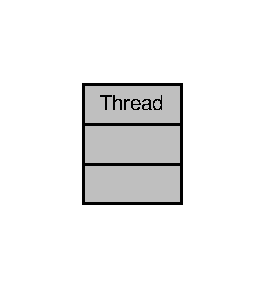
\includegraphics[width=127pt]{class_thread__coll__graph}
\end{center}
\end{figure}


La documentation de cette classe a été générée à partir du fichier suivant \+:\begin{DoxyCompactItemize}
\item 
\hyperlink{_liaison_bluetooth_8java}{Liaison\+Bluetooth.\+java}\end{DoxyCompactItemize}

\hypertarget{classcom_1_1example_1_1area_1_1_liaison_bluetooth_1_1_t_reception}{}\subsection{Référence de la classe com.\+example.\+area.\+Liaison\+Bluetooth.\+T\+Reception}
\label{classcom_1_1example_1_1area_1_1_liaison_bluetooth_1_1_t_reception}\index{com.\+example.\+area.\+Liaison\+Bluetooth.\+T\+Reception@{com.\+example.\+area.\+Liaison\+Bluetooth.\+T\+Reception}}


Graphe de collaboration de com.\+example.\+area.\+Liaison\+Bluetooth.\+T\+Reception\+:
\nopagebreak
\begin{figure}[H]
\begin{center}
\leavevmode
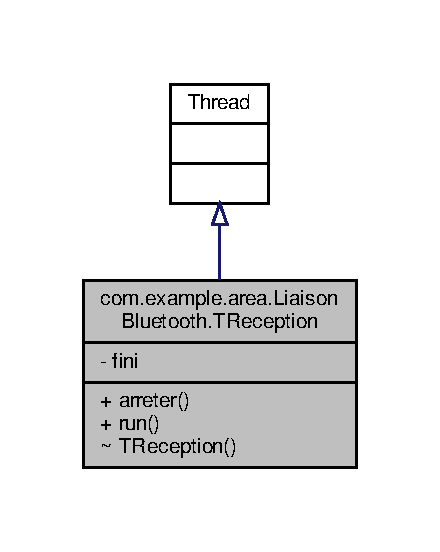
\includegraphics[width=211pt]{classcom_1_1example_1_1area_1_1_liaison_bluetooth_1_1_t_reception__coll__graph}
\end{center}
\end{figure}
\subsubsection*{Fonctions membres publiques}
\begin{DoxyCompactItemize}
\item 
void \hyperlink{classcom_1_1example_1_1area_1_1_liaison_bluetooth_1_1_t_reception_a89f97f22a976b8632e82b2aa94ab2674}{arreter} ()
\begin{DoxyCompactList}\small\item\em Méthode qui permet d\textquotesingle{}arrêter lire les données entrantes. \end{DoxyCompactList}\item 
void \hyperlink{classcom_1_1example_1_1area_1_1_liaison_bluetooth_1_1_t_reception_afb141736dac915d0c82f96f75033f318}{run} ()
\begin{DoxyCompactList}\small\item\em Méthode qui permet de lire les données entrantes. \end{DoxyCompactList}\end{DoxyCompactItemize}
\subsubsection*{Attributs privés}
\begin{DoxyCompactItemize}
\item 
boolean \hyperlink{classcom_1_1example_1_1area_1_1_liaison_bluetooth_1_1_t_reception_a7f942e7af3e97af754f2591d2bd20435}{fini}
\end{DoxyCompactItemize}


\subsubsection{Description détaillée}


Définition à la ligne \hyperlink{_liaison_bluetooth_8java_source_l00228}{228} du fichier \hyperlink{_liaison_bluetooth_8java_source}{Liaison\+Bluetooth.\+java}.



\subsubsection{Documentation des fonctions membres}
\mbox{\Hypertarget{classcom_1_1example_1_1area_1_1_liaison_bluetooth_1_1_t_reception_a89f97f22a976b8632e82b2aa94ab2674}\label{classcom_1_1example_1_1area_1_1_liaison_bluetooth_1_1_t_reception_a89f97f22a976b8632e82b2aa94ab2674}} 
\index{com\+::example\+::area\+::\+Liaison\+Bluetooth\+::\+T\+Reception@{com\+::example\+::area\+::\+Liaison\+Bluetooth\+::\+T\+Reception}!arreter@{arreter}}
\index{arreter@{arreter}!com\+::example\+::area\+::\+Liaison\+Bluetooth\+::\+T\+Reception@{com\+::example\+::area\+::\+Liaison\+Bluetooth\+::\+T\+Reception}}
\paragraph{\texorpdfstring{arreter()}{arreter()}}
{\footnotesize\ttfamily void com.\+example.\+area.\+Liaison\+Bluetooth.\+T\+Reception.\+arreter (\begin{DoxyParamCaption}{ }\end{DoxyParamCaption})}



Méthode qui permet d\textquotesingle{}arrêter lire les données entrantes. 



Définition à la ligne \hyperlink{_liaison_bluetooth_8java_source_l00287}{287} du fichier \hyperlink{_liaison_bluetooth_8java_source}{Liaison\+Bluetooth.\+java}.



Référencé par \hyperlink{_liaison_bluetooth_8java_source_l00171}{com.\+example.\+area.\+Liaison\+Bluetooth.\+deconnecter()}.


\begin{DoxyCode}
00288         \{
00289             \textcolor{keywordflow}{if} (\hyperlink{classcom_1_1example_1_1area_1_1_liaison_bluetooth_1_1_t_reception_a7f942e7af3e97af754f2591d2bd20435}{fini} == \textcolor{keyword}{false})
00290             \{
00291                 \hyperlink{classcom_1_1example_1_1area_1_1_liaison_bluetooth_1_1_t_reception_a7f942e7af3e97af754f2591d2bd20435}{fini} = \textcolor{keyword}{true};
00292             \}
00293 
00294             \textcolor{keywordflow}{try}
00295             \{
00296                 \hyperlink{class_thread}{Thread}.sleep(250);
00297             \}
00298             \textcolor{keywordflow}{catch} (InterruptedException e)
00299             \{
00300                 e.printStackTrace();
00301             \}
00302         \}
\end{DoxyCode}
\mbox{\Hypertarget{classcom_1_1example_1_1area_1_1_liaison_bluetooth_1_1_t_reception_afb141736dac915d0c82f96f75033f318}\label{classcom_1_1example_1_1area_1_1_liaison_bluetooth_1_1_t_reception_afb141736dac915d0c82f96f75033f318}} 
\index{com\+::example\+::area\+::\+Liaison\+Bluetooth\+::\+T\+Reception@{com\+::example\+::area\+::\+Liaison\+Bluetooth\+::\+T\+Reception}!run@{run}}
\index{run@{run}!com\+::example\+::area\+::\+Liaison\+Bluetooth\+::\+T\+Reception@{com\+::example\+::area\+::\+Liaison\+Bluetooth\+::\+T\+Reception}}
\paragraph{\texorpdfstring{run()}{run()}}
{\footnotesize\ttfamily void com.\+example.\+area.\+Liaison\+Bluetooth.\+T\+Reception.\+run (\begin{DoxyParamCaption}{ }\end{DoxyParamCaption})}



Méthode qui permet de lire les données entrantes. 



Définition à la ligne \hyperlink{_liaison_bluetooth_8java_source_l00240}{240} du fichier \hyperlink{_liaison_bluetooth_8java_source}{Liaison\+Bluetooth.\+java}.



Références \hyperlink{_liaison_bluetooth_8java_source_l00136}{com.\+example.\+area.\+Liaison\+Bluetooth.\+connecter()}, \hyperlink{_liaison_bluetooth_8java_source_l00037}{com.\+example.\+area.\+Liaison\+Bluetooth.\+D\+E\+C\+O\+N\+N\+E\+X\+I\+O\+N\+\_\+\+S\+O\+C\+K\+ET}, et \hyperlink{_liaison_bluetooth_8java_source_l00038}{com.\+example.\+area.\+Liaison\+Bluetooth.\+R\+E\+C\+E\+P\+T\+I\+O\+N\+\_\+\+T\+R\+A\+ME}.


\begin{DoxyCode}
00241         \{
00242             Log.d(\hyperlink{classcom_1_1example_1_1area_1_1_liaison_bluetooth_ac51aa4b63fae5c36734a061cc05d7fc9}{TAG},\textcolor{stringliteral}{"Démarrage du thread Réception pour le module "} + 
      \hyperlink{classcom_1_1example_1_1area_1_1_liaison_bluetooth_a80068a7178f6c84eae7bab50cf0a784a}{module}.getName() + \textcolor{stringliteral}{" | Adresse : "} + \hyperlink{classcom_1_1example_1_1area_1_1_liaison_bluetooth_a80068a7178f6c84eae7bab50cf0a784a}{module}.getAddress());
00243             BufferedReader reception = \textcolor{keyword}{new} BufferedReader(\textcolor{keyword}{new} InputStreamReader(
      \hyperlink{classcom_1_1example_1_1area_1_1_liaison_bluetooth_a9a3a7d77bae06a972782b6e73471878d}{fluxReception}));
00244             \textcolor{keywordflow}{while}(!\hyperlink{classcom_1_1example_1_1area_1_1_liaison_bluetooth_1_1_t_reception_a7f942e7af3e97af754f2591d2bd20435}{fini})
00245             \{
00246                 \textcolor{keywordflow}{try}
00247                 \{
00248                     String trame = \textcolor{stringliteral}{""};
00249                     \textcolor{keywordflow}{if} (\hyperlink{classcom_1_1example_1_1area_1_1_liaison_bluetooth_ab59b57f5e59d0236e49ecf68c053cb27}{socket}.isConnected())
00250                     \{
00251                         trame = reception.readLine();
00252                         \textcolor{keywordflow}{if}(trame.length() > 0)
00253                         \{
00254                           Log.d(\hyperlink{classcom_1_1example_1_1area_1_1_liaison_bluetooth_ac51aa4b63fae5c36734a061cc05d7fc9}{TAG}, \textcolor{stringliteral}{"Trame : "} + trame);
00255                           Message message = \textcolor{keyword}{new} Message();
00256                           message.what = \hyperlink{classcom_1_1example_1_1area_1_1_liaison_bluetooth_a1a3058c683cec15fe0f3699f7fc26073}{RECEPTION\_TRAME};
00257                           message.obj = trame;
00258                           \hyperlink{classcom_1_1example_1_1area_1_1_liaison_bluetooth_ace2c20759fc96d3ae787f1f726fd2691}{handlerIHM}.sendMessage(message);
00259                         \}
00260                     \}
00261                 \}
00262                 \textcolor{keywordflow}{catch} (IOException e)
00263                 \{
00264                     e.printStackTrace();
00265                     Message message = \textcolor{keyword}{new} Message();
00266                     message.what = \hyperlink{classcom_1_1example_1_1area_1_1_liaison_bluetooth_a8ff08468d7b2cead9c3714c665f75d0e}{DECONNEXION\_SOCKET};
00267                     message.obj = \hyperlink{classcom_1_1example_1_1area_1_1_liaison_bluetooth_a80068a7178f6c84eae7bab50cf0a784a}{module}.getName();
00268                     \hyperlink{classcom_1_1example_1_1area_1_1_liaison_bluetooth_ace2c20759fc96d3ae787f1f726fd2691}{handlerIHM}.sendMessage(message);
00269                     \hyperlink{classcom_1_1example_1_1area_1_1_liaison_bluetooth_a7b9662a4224762b23c814d1f4539002a}{connecter}();
00270                 \}
00271 
00272                 \textcolor{keywordflow}{try}
00273                 \{
00274                     \hyperlink{class_thread}{Thread}.sleep(250);
00275                 \}
00276                 \textcolor{keywordflow}{catch} (InterruptedException e)
00277                 \{
00278                     e.printStackTrace();
00279                 \}
00280             \}
00281             Log.d(\hyperlink{classcom_1_1example_1_1area_1_1_liaison_bluetooth_ac51aa4b63fae5c36734a061cc05d7fc9}{TAG},\textcolor{stringliteral}{"Arrêt du thread Réception pour le module "} + \hyperlink{classcom_1_1example_1_1area_1_1_liaison_bluetooth_a80068a7178f6c84eae7bab50cf0a784a}{module}.getName() + \textcolor{stringliteral}{" | Adresse
       : "} + \hyperlink{classcom_1_1example_1_1area_1_1_liaison_bluetooth_a80068a7178f6c84eae7bab50cf0a784a}{module}.getAddress());
00282         \}
\end{DoxyCode}


\subsubsection{Documentation des données membres}
\mbox{\Hypertarget{classcom_1_1example_1_1area_1_1_liaison_bluetooth_1_1_t_reception_a7f942e7af3e97af754f2591d2bd20435}\label{classcom_1_1example_1_1area_1_1_liaison_bluetooth_1_1_t_reception_a7f942e7af3e97af754f2591d2bd20435}} 
\index{com\+::example\+::area\+::\+Liaison\+Bluetooth\+::\+T\+Reception@{com\+::example\+::area\+::\+Liaison\+Bluetooth\+::\+T\+Reception}!fini@{fini}}
\index{fini@{fini}!com\+::example\+::area\+::\+Liaison\+Bluetooth\+::\+T\+Reception@{com\+::example\+::area\+::\+Liaison\+Bluetooth\+::\+T\+Reception}}
\paragraph{\texorpdfstring{fini}{fini}}
{\footnotesize\ttfamily boolean com.\+example.\+area.\+Liaison\+Bluetooth.\+T\+Reception.\+fini\hspace{0.3cm}{\ttfamily [private]}}



Définition à la ligne \hyperlink{_liaison_bluetooth_8java_source_l00230}{230} du fichier \hyperlink{_liaison_bluetooth_8java_source}{Liaison\+Bluetooth.\+java}.



La documentation de cette classe a été générée à partir du fichier suivant \+:\begin{DoxyCompactItemize}
\item 
\hyperlink{_liaison_bluetooth_8java}{Liaison\+Bluetooth.\+java}\end{DoxyCompactItemize}

\section{Documentation des fichiers}
\hypertarget{_base_de_donnees_8java}{}\subsection{Référence du fichier Base\+De\+Donnees.\+java}
\label{_base_de_donnees_8java}\index{Base\+De\+Donnees.\+java@{Base\+De\+Donnees.\+java}}
\subsubsection*{Classes}
\begin{DoxyCompactItemize}
\item 
class \hyperlink{classcom_1_1example_1_1area_1_1_base_de_donnees}{com.\+example.\+area.\+Base\+De\+Donnees}
\end{DoxyCompactItemize}
\subsubsection*{Paquetages}
\begin{DoxyCompactItemize}
\item 
package \hyperlink{namespacecom_1_1example_1_1area}{com.\+example.\+area}
\end{DoxyCompactItemize}

\hypertarget{_base_de_donnees_8java_source}{}\subsection{Base\+De\+Donnees.\+java}
\label{_base_de_donnees_8java_source}\index{Base\+De\+Donnees.\+java@{Base\+De\+Donnees.\+java}}

\begin{DoxyCode}
\Hypertarget{_base_de_donnees_8java_source_l00001}\hyperlink{namespacecom_1_1example_1_1area}{00001} \textcolor{keyword}{package }com.example.area;
00002 
\Hypertarget{_base_de_donnees_8java_source_l00011}\hyperlink{classcom_1_1example_1_1area_1_1_base_de_donnees}{00011} \textcolor{keyword}{public} \textcolor{keyword}{class }\hyperlink{classcom_1_1example_1_1area_1_1_base_de_donnees}{BaseDeDonnees}
00012 \{
\Hypertarget{_base_de_donnees_8java_source_l00013}\hyperlink{classcom_1_1example_1_1area_1_1_base_de_donnees_af9165ddf75f87c6f54c08159b5f791ce}{00013}   \textcolor{keyword}{public} \hyperlink{classcom_1_1example_1_1area_1_1_base_de_donnees_af9165ddf75f87c6f54c08159b5f791ce}{BaseDeDonnees}()
00014   \{
00015   \}
00016 
\Hypertarget{_base_de_donnees_8java_source_l00017}\hyperlink{classcom_1_1example_1_1area_1_1_base_de_donnees_a71c0a57c6fe4a5097e4d4c7ef1585cf3}{00017}   \textcolor{keyword}{public} \textcolor{keywordtype}{void} \hyperlink{classcom_1_1example_1_1area_1_1_base_de_donnees_a71c0a57c6fe4a5097e4d4c7ef1585cf3}{ouvrir}()
00018   \{
00019   \}
00020 
\Hypertarget{_base_de_donnees_8java_source_l00021}\hyperlink{classcom_1_1example_1_1area_1_1_base_de_donnees_ad51319bd8b62ebf33d33d6f3b8347d41}{00021}   \textcolor{keyword}{public} \textcolor{keywordtype}{void} \hyperlink{classcom_1_1example_1_1area_1_1_base_de_donnees_ad51319bd8b62ebf33d33d6f3b8347d41}{fermer}()
00022   \{
00023   \}
00024 
\Hypertarget{_base_de_donnees_8java_source_l00025}\hyperlink{classcom_1_1example_1_1area_1_1_base_de_donnees_adf1ed72483551ccae7812eec115b9bb7}{00025}   \textcolor{keyword}{public} \textcolor{keywordtype}{void} \hyperlink{classcom_1_1example_1_1area_1_1_base_de_donnees_adf1ed72483551ccae7812eec115b9bb7}{envoyer}(String requete)
00026   \{
00027   \}
00028 
00029 \}
\end{DoxyCode}

\hypertarget{_equipe_8java}{}\subsection{Référence du fichier Equipe.\+java}
\label{_equipe_8java}\index{Equipe.\+java@{Equipe.\+java}}


Déclaration de la classe Equipe.  


\subsubsection*{Classes}
\begin{DoxyCompactItemize}
\item 
class \hyperlink{classcom_1_1example_1_1area_1_1_equipe}{com.\+example.\+area.\+Equipe}
\end{DoxyCompactItemize}
\subsubsection*{Paquetages}
\begin{DoxyCompactItemize}
\item 
package \hyperlink{namespacecom_1_1example_1_1area}{com.\+example.\+area}
\end{DoxyCompactItemize}


\subsubsection{Description détaillée}
Déclaration de la classe Equipe. 

\begin{DoxyAuthor}{Auteur}
B\+R\+U\+N\+ET Bastien \$\+Last\+Changed\+Revision\$ \$\+Last\+Changed\+Date\$ 
\end{DoxyAuthor}


Définition dans le fichier \hyperlink{_equipe_8java_source}{Equipe.\+java}.


\hypertarget{_equipe_8java_source}{}\subsection{Equipe.\+java}
\label{_equipe_8java_source}\index{Equipe.\+java@{Equipe.\+java}}

\begin{DoxyCode}
00001 \textcolor{keyword}{package }com.example.area;
00002 
00003 \textcolor{keyword}{import} java.util.Vector;
00004 
\Hypertarget{_equipe_8java_source_l00013}\hyperlink{classcom_1_1example_1_1area_1_1_equipe}{00013} \textcolor{keyword}{public} \textcolor{keyword}{class }\hyperlink{classcom_1_1example_1_1area_1_1_equipe}{Equipe}
00014 \{
\Hypertarget{_equipe_8java_source_l00015}\hyperlink{classcom_1_1example_1_1area_1_1_equipe_a3b61c78bfb4284470bc3b5315b6b03e7}{00015}     \textcolor{keyword}{public} \textcolor{keyword}{static} \textcolor{keyword}{final} \textcolor{keywordtype}{int} \hyperlink{classcom_1_1example_1_1area_1_1_equipe_a3b61c78bfb4284470bc3b5315b6b03e7}{INDEX\_JOUEUR\_A} = 0;
\Hypertarget{_equipe_8java_source_l00016}\hyperlink{classcom_1_1example_1_1area_1_1_equipe_a1b9c3f1c23757be40472c63504df9d37}{00016}     \textcolor{keyword}{public} \textcolor{keyword}{static} \textcolor{keyword}{final} \textcolor{keywordtype}{int} \hyperlink{classcom_1_1example_1_1area_1_1_equipe_a1b9c3f1c23757be40472c63504df9d37}{INDEX\_JOUEUR\_B} = 1;
\Hypertarget{_equipe_8java_source_l00017}\hyperlink{classcom_1_1example_1_1area_1_1_equipe_abbd44b4789c0234d86578fbbfd8bf624}{00017}     \textcolor{keyword}{public} \textcolor{keyword}{static} \textcolor{keyword}{final} \textcolor{keywordtype}{int} \hyperlink{classcom_1_1example_1_1area_1_1_equipe_abbd44b4789c0234d86578fbbfd8bf624}{INDEX\_JOUEUR\_C} = 2;
\Hypertarget{_equipe_8java_source_l00018}\hyperlink{classcom_1_1example_1_1area_1_1_equipe_ae204f48df7446d745f33ff4a7e662ea7}{00018}     \textcolor{keyword}{public} \textcolor{keyword}{static} \textcolor{keyword}{final} \textcolor{keywordtype}{int} \hyperlink{classcom_1_1example_1_1area_1_1_equipe_ae204f48df7446d745f33ff4a7e662ea7}{INDEX\_JOUEUR\_D} = 3;
00019 
\Hypertarget{_equipe_8java_source_l00020}\hyperlink{classcom_1_1example_1_1area_1_1_equipe_aeca3d6f47e05b7c2aef70b64778d5d47}{00020}     \textcolor{keyword}{public} \textcolor{keyword}{static} \textcolor{keyword}{final} \textcolor{keywordtype}{int} \hyperlink{classcom_1_1example_1_1area_1_1_equipe_aeca3d6f47e05b7c2aef70b64778d5d47}{INDEX\_JOUEUR\_W} = 0;
\Hypertarget{_equipe_8java_source_l00021}\hyperlink{classcom_1_1example_1_1area_1_1_equipe_ae5f0313dce371f13950d4fdc54074dd9}{00021}     \textcolor{keyword}{public} \textcolor{keyword}{static} \textcolor{keyword}{final} \textcolor{keywordtype}{int} \hyperlink{classcom_1_1example_1_1area_1_1_equipe_ae5f0313dce371f13950d4fdc54074dd9}{INDEX\_JOUEUR\_X} = 1;
\Hypertarget{_equipe_8java_source_l00022}\hyperlink{classcom_1_1example_1_1area_1_1_equipe_a11d252140fc4e3edd71a31573221a7b7}{00022}     \textcolor{keyword}{public} \textcolor{keyword}{static} \textcolor{keyword}{final} \textcolor{keywordtype}{int} \hyperlink{classcom_1_1example_1_1area_1_1_equipe_a11d252140fc4e3edd71a31573221a7b7}{INDEX\_JOUEUR\_Y} = 2;
\Hypertarget{_equipe_8java_source_l00023}\hyperlink{classcom_1_1example_1_1area_1_1_equipe_a50e1c2cbd7d24c8c5b4f0f4de1652621}{00023}     \textcolor{keyword}{public} \textcolor{keyword}{static} \textcolor{keyword}{final} \textcolor{keywordtype}{int} \hyperlink{classcom_1_1example_1_1area_1_1_equipe_a50e1c2cbd7d24c8c5b4f0f4de1652621}{INDEX\_JOUEUR\_Z} = 3;
00024 
\Hypertarget{_equipe_8java_source_l00025}\hyperlink{classcom_1_1example_1_1area_1_1_equipe_af01e154be3aaa3fbcf909c3a44734b2e}{00025}     \textcolor{keyword}{private} \textcolor{keywordtype}{int} \hyperlink{classcom_1_1example_1_1area_1_1_equipe_af01e154be3aaa3fbcf909c3a44734b2e}{nbPartiesGagnees};
\Hypertarget{_equipe_8java_source_l00026}\hyperlink{classcom_1_1example_1_1area_1_1_equipe_ac93205e041df88192dd6b1dfc8488e0a}{00026}     \textcolor{keyword}{private} String \hyperlink{classcom_1_1example_1_1area_1_1_equipe_ac93205e041df88192dd6b1dfc8488e0a}{nomClub};
\Hypertarget{_equipe_8java_source_l00027}\hyperlink{classcom_1_1example_1_1area_1_1_equipe_a13f5e9288dec5f11829e1a7ccc21cdc9}{00027}     \textcolor{keyword}{private} Vector<Joueur> \hyperlink{classcom_1_1example_1_1area_1_1_equipe_a13f5e9288dec5f11829e1a7ccc21cdc9}{joueurs};
\Hypertarget{_equipe_8java_source_l00028}\hyperlink{classcom_1_1example_1_1area_1_1_equipe_a3be17f443cb57269d595d8b860acc66a}{00028}     \textcolor{keyword}{private} \textcolor{keywordtype}{int} \hyperlink{classcom_1_1example_1_1area_1_1_equipe_a3be17f443cb57269d595d8b860acc66a}{id};
00029 
\Hypertarget{_equipe_8java_source_l00030}\hyperlink{classcom_1_1example_1_1area_1_1_equipe_a313ec6933f3fb30f68ec93c7c290c6ee}{00030}     \textcolor{keyword}{public} \hyperlink{classcom_1_1example_1_1area_1_1_equipe_a313ec6933f3fb30f68ec93c7c290c6ee}{Equipe}(String nomClub, Vector<Joueur> joueurs)
00031     \{
00032         this.nbPartiesGagnees = 0;
00033         this.nomClub = \hyperlink{classcom_1_1example_1_1area_1_1_equipe_ac93205e041df88192dd6b1dfc8488e0a}{nomClub};
00034         this.joueurs = \hyperlink{classcom_1_1example_1_1area_1_1_equipe_a13f5e9288dec5f11829e1a7ccc21cdc9}{joueurs};
00035         this.\textcolor{keywordtype}{id} = 0;
00036     \}
00037 
\Hypertarget{_equipe_8java_source_l00038}\hyperlink{classcom_1_1example_1_1area_1_1_equipe_a1ba6f14b9b168e283d5d6417ad0a5ed2}{00038}     \textcolor{keyword}{public} \textcolor{keyword}{final} \textcolor{keywordtype}{int} \hyperlink{classcom_1_1example_1_1area_1_1_equipe_a1ba6f14b9b168e283d5d6417ad0a5ed2}{getNbPartiesGagnees}()
00039     \{
00040       \textcolor{keywordflow}{return} \hyperlink{classcom_1_1example_1_1area_1_1_equipe_af01e154be3aaa3fbcf909c3a44734b2e}{nbPartiesGagnees};
00041     \}
00042 
\Hypertarget{_equipe_8java_source_l00043}\hyperlink{classcom_1_1example_1_1area_1_1_equipe_a735e5e0aaac9ac2c17f3eca3d47862dc}{00043}     \textcolor{keyword}{public} \textcolor{keyword}{final} String \hyperlink{classcom_1_1example_1_1area_1_1_equipe_a735e5e0aaac9ac2c17f3eca3d47862dc}{getNomClub}()
00044     \{
00045       \textcolor{keywordflow}{return} \hyperlink{classcom_1_1example_1_1area_1_1_equipe_ac93205e041df88192dd6b1dfc8488e0a}{nomClub};
00046     \}
00047 
\Hypertarget{_equipe_8java_source_l00048}\hyperlink{classcom_1_1example_1_1area_1_1_equipe_aba16e2f2a922d1b2c4219dc6c865482c}{00048}     \textcolor{keyword}{public} \textcolor{keywordtype}{void} \hyperlink{classcom_1_1example_1_1area_1_1_equipe_aba16e2f2a922d1b2c4219dc6c865482c}{setNbPartiesGagnees}(\textcolor{keywordtype}{int} nbPartiesGagnees)
00049     \{
00050       this.nbPartiesGagnees = \hyperlink{classcom_1_1example_1_1area_1_1_equipe_af01e154be3aaa3fbcf909c3a44734b2e}{nbPartiesGagnees};
00051     \}
00052 
\Hypertarget{_equipe_8java_source_l00053}\hyperlink{classcom_1_1example_1_1area_1_1_equipe_aa681b4ea72d93a16fc8384fa3ccc8b21}{00053}     \textcolor{keyword}{public} Vector<Joueur> \hyperlink{classcom_1_1example_1_1area_1_1_equipe_aa681b4ea72d93a16fc8384fa3ccc8b21}{getJoueurs}()
00054     \{
00055         \textcolor{keywordflow}{return} \hyperlink{classcom_1_1example_1_1area_1_1_equipe_a13f5e9288dec5f11829e1a7ccc21cdc9}{joueurs};
00056     \}
00057 
00058 \}
\end{DoxyCode}

\hypertarget{_i_h_m_gestion_partie_8java}{}\subsection{Référence du fichier I\+H\+M\+Gestion\+Partie.\+java}
\label{_i_h_m_gestion_partie_8java}\index{I\+H\+M\+Gestion\+Partie.\+java@{I\+H\+M\+Gestion\+Partie.\+java}}


Déclaration de la classe I\+H\+M\+Gestion\+Partie.  


\subsubsection*{Classes}
\begin{DoxyCompactItemize}
\item 
class \hyperlink{classcom_1_1example_1_1area_1_1_i_h_m_gestion_partie}{com.\+example.\+area.\+I\+H\+M\+Gestion\+Partie}
\begin{DoxyCompactList}\small\item\em L\textquotesingle{}activité de gestion d\textquotesingle{}une partie de l\textquotesingle{}application A\+R\+EA. \end{DoxyCompactList}\end{DoxyCompactItemize}
\subsubsection*{Paquetages}
\begin{DoxyCompactItemize}
\item 
package \hyperlink{namespacecom_1_1example_1_1area}{com.\+example.\+area}
\end{DoxyCompactItemize}


\subsubsection{Description détaillée}
Déclaration de la classe I\+H\+M\+Gestion\+Partie. 

\begin{DoxyAuthor}{Auteur}
B\+R\+U\+N\+ET Bastien \$\+Last\+Changed\+Revision\$ \$\+Last\+Changed\+Date\$ 
\end{DoxyAuthor}


Définition dans le fichier \hyperlink{_i_h_m_gestion_partie_8java_source}{I\+H\+M\+Gestion\+Partie.\+java}.


\hypertarget{_i_h_m_gestion_partie_8java_source}{}\subsection{I\+H\+M\+Gestion\+Partie.\+java}
\label{_i_h_m_gestion_partie_8java_source}\index{I\+H\+M\+Gestion\+Partie.\+java@{I\+H\+M\+Gestion\+Partie.\+java}}

\begin{DoxyCode}
00001 \textcolor{keyword}{package }com.example.area;
00002 
00003 \textcolor{keyword}{import} androidx.annotation.ColorRes;
00004 \textcolor{keyword}{import} androidx.annotation.NonNull;
00005 \textcolor{keyword}{import} androidx.appcompat.app.ActionBar;
00006 \textcolor{keyword}{import} androidx.appcompat.app.AppCompatActivity;
00007 \textcolor{keyword}{import} androidx.appcompat.widget.Toolbar;
00008 
00009 \textcolor{keyword}{import} android.app.AlertDialog;
00010 \textcolor{keyword}{import} android.bluetooth.BluetoothAdapter;
00011 \textcolor{keyword}{import} android.bluetooth.BluetoothDevice;
00012 \textcolor{keyword}{import} android.content.DialogInterface;
00013 \textcolor{keyword}{import} android.content.Intent;
00014 \textcolor{keyword}{import} android.graphics.Color;
00015 \textcolor{keyword}{import} android.os.Bundle;
00016 \textcolor{keyword}{import} android.os.Handler;
00017 \textcolor{keyword}{import} android.os.Message;
00018 \textcolor{keyword}{import} android.util.Log;
00019 \textcolor{keyword}{import} android.view.Gravity;
00020 \textcolor{keyword}{import} android.view.LayoutInflater;
00021 \textcolor{keyword}{import} android.view.Menu;
00022 \textcolor{keyword}{import} android.view.MenuItem;
00023 \textcolor{keyword}{import} android.view.View;
00024 \textcolor{keyword}{import} android.widget.Button;
00025 \textcolor{keyword}{import} android.widget.ImageView;
00026 \textcolor{keyword}{import} android.widget.TextView;
00027 \textcolor{keyword}{import} android.widget.Toast;
00028 
00029 \textcolor{keyword}{import} java.lang.reflect.Array;
00030 \textcolor{keyword}{import} java.util.Set;
00031 \textcolor{keyword}{import} java.util.Vector;
00032 
00033 \textcolor{comment}{// Pour Logcat : \_IHMGestionRencontre|\_IHMGestionPartie|\_Partie|\_LiaisonBluetooth|\_ProtocoleAREA}
00034 
\Hypertarget{_i_h_m_gestion_partie_8java_source_l00047}\hyperlink{classcom_1_1example_1_1area_1_1_i_h_m_gestion_partie}{00047} \textcolor{keyword}{public} \textcolor{keyword}{class }\hyperlink{classcom_1_1example_1_1area_1_1_i_h_m_gestion_partie}{IHMGestionPartie} \textcolor{keyword}{extends} AppCompatActivity
00048 \{
\Hypertarget{_i_h_m_gestion_partie_8java_source_l00052}\hyperlink{classcom_1_1example_1_1area_1_1_i_h_m_gestion_partie_a78af1eb84e4a48b7f69c3ebee193933c}{00052}     \textcolor{keyword}{private} \textcolor{keyword}{static} \textcolor{keyword}{final} String \hyperlink{classcom_1_1example_1_1area_1_1_i_h_m_gestion_partie_a78af1eb84e4a48b7f69c3ebee193933c}{TAG} = \textcolor{stringliteral}{"\_IHMGestionPartie"};  
\Hypertarget{_i_h_m_gestion_partie_8java_source_l00053}\hyperlink{classcom_1_1example_1_1area_1_1_i_h_m_gestion_partie_abc36e82bb3c4a2fb719305ea9e525c9b}{00053}     \textcolor{keyword}{private} \textcolor{keyword}{static} \textcolor{keyword}{final} String \hyperlink{classcom_1_1example_1_1area_1_1_i_h_m_gestion_partie_abc36e82bb3c4a2fb719305ea9e525c9b}{TEXTE\_BOUTON\_TEMPS\_MORT} = \textcolor{stringliteral}{"Temps mort"};
\Hypertarget{_i_h_m_gestion_partie_8java_source_l00054}\hyperlink{classcom_1_1example_1_1area_1_1_i_h_m_gestion_partie_a9218ba4464b7631738927d74539ac927}{00054}     \textcolor{keyword}{private} \textcolor{keyword}{static} \textcolor{keyword}{final} String \hyperlink{classcom_1_1example_1_1area_1_1_i_h_m_gestion_partie_a9218ba4464b7631738927d74539ac927}{TEXTE\_BOUTON\_RETIRER\_POINT} = \textcolor{stringliteral}{"-1"};
\Hypertarget{_i_h_m_gestion_partie_8java_source_l00055}\hyperlink{classcom_1_1example_1_1area_1_1_i_h_m_gestion_partie_a29eb33d17f8f318937bd01705f5769d8}{00055}     \textcolor{keyword}{private} \textcolor{keyword}{static} \textcolor{keyword}{final} String \hyperlink{classcom_1_1example_1_1area_1_1_i_h_m_gestion_partie_a29eb33d17f8f318937bd01705f5769d8}{TEXTE\_BOUTON\_AJOUTER\_POINT} = \textcolor{stringliteral}{"+1"};
\Hypertarget{_i_h_m_gestion_partie_8java_source_l00056}\hyperlink{classcom_1_1example_1_1area_1_1_i_h_m_gestion_partie_aa5b1cdff8bb4d6f6157ae215f43062c5}{00056}     \textcolor{keyword}{private} \textcolor{keyword}{static} \textcolor{keyword}{final} String \hyperlink{classcom_1_1example_1_1area_1_1_i_h_m_gestion_partie_aa5b1cdff8bb4d6f6157ae215f43062c5}{TEXTE\_TOAST\_NET} = \textcolor{stringliteral}{"NET"};
\Hypertarget{_i_h_m_gestion_partie_8java_source_l00057}\hyperlink{classcom_1_1example_1_1area_1_1_i_h_m_gestion_partie_a12cdd76d3c9dec83783e40a0d017ac17}{00057}     \textcolor{keyword}{private} \textcolor{keyword}{static} \textcolor{keyword}{final} String \hyperlink{classcom_1_1example_1_1area_1_1_i_h_m_gestion_partie_a12cdd76d3c9dec83783e40a0d017ac17}{TEXTE\_CONNEXION\_MODULE\_NET} = \textcolor{stringliteral}{"Module NET "};
\Hypertarget{_i_h_m_gestion_partie_8java_source_l00058}\hyperlink{classcom_1_1example_1_1area_1_1_i_h_m_gestion_partie_a60d4b79c44e29fe68c565cf24ed6a22a}{00058}     \textcolor{keyword}{private} \textcolor{keyword}{static} \textcolor{keyword}{final} String \hyperlink{classcom_1_1example_1_1area_1_1_i_h_m_gestion_partie_a60d4b79c44e29fe68c565cf24ed6a22a}{TEXTE\_CONNEXION\_MODULE\_AFFICHEUR} = \textcolor{stringliteral}{"Module
       Afficheur "};
00059 
\Hypertarget{_i_h_m_gestion_partie_8java_source_l00063}\hyperlink{classcom_1_1example_1_1area_1_1_i_h_m_gestion_partie_ad7ac57a177098fba4ba7ea29a2418f10}{00063}     \textcolor{keyword}{private} TextView \hyperlink{classcom_1_1example_1_1area_1_1_i_h_m_gestion_partie_ad7ac57a177098fba4ba7ea29a2418f10}{nomJoueurA};
\Hypertarget{_i_h_m_gestion_partie_8java_source_l00064}\hyperlink{classcom_1_1example_1_1area_1_1_i_h_m_gestion_partie_a9a5b0bc9c6f1d865b85bfe789219e16e}{00064}     \textcolor{keyword}{private} TextView \hyperlink{classcom_1_1example_1_1area_1_1_i_h_m_gestion_partie_a9a5b0bc9c6f1d865b85bfe789219e16e}{prenomJoueurA};
\Hypertarget{_i_h_m_gestion_partie_8java_source_l00065}\hyperlink{classcom_1_1example_1_1area_1_1_i_h_m_gestion_partie_a00dbc2ac1396af550520dd011d8e01cc}{00065}     \textcolor{keyword}{private} TextView \hyperlink{classcom_1_1example_1_1area_1_1_i_h_m_gestion_partie_a00dbc2ac1396af550520dd011d8e01cc}{nomDeuxiemeJoueurA};
\Hypertarget{_i_h_m_gestion_partie_8java_source_l00066}\hyperlink{classcom_1_1example_1_1area_1_1_i_h_m_gestion_partie_af209e9cda709137d8b77170a35b295e0}{00066}     \textcolor{keyword}{private} TextView \hyperlink{classcom_1_1example_1_1area_1_1_i_h_m_gestion_partie_af209e9cda709137d8b77170a35b295e0}{prenomDeuxiemeJoueurA};
\Hypertarget{_i_h_m_gestion_partie_8java_source_l00067}\hyperlink{classcom_1_1example_1_1area_1_1_i_h_m_gestion_partie_af59fb470e464a16a7f09f4440b18c2e8}{00067}     \textcolor{keyword}{private} Button \hyperlink{classcom_1_1example_1_1area_1_1_i_h_m_gestion_partie_af59fb470e464a16a7f09f4440b18c2e8}{boutonRetirerPointJoueurA};
\Hypertarget{_i_h_m_gestion_partie_8java_source_l00068}\hyperlink{classcom_1_1example_1_1area_1_1_i_h_m_gestion_partie_aa99f420624fb6c990516b30ebe0805cc}{00068}     \textcolor{keyword}{private} Button \hyperlink{classcom_1_1example_1_1area_1_1_i_h_m_gestion_partie_aa99f420624fb6c990516b30ebe0805cc}{boutonAjouterPointJoueurA};
\Hypertarget{_i_h_m_gestion_partie_8java_source_l00069}\hyperlink{classcom_1_1example_1_1area_1_1_i_h_m_gestion_partie_a811fe6ba189ad62350a6e95c3147a1f0}{00069}     \textcolor{keyword}{private} ImageView \hyperlink{classcom_1_1example_1_1area_1_1_i_h_m_gestion_partie_a811fe6ba189ad62350a6e95c3147a1f0}{imageServeurJoueurA};
\Hypertarget{_i_h_m_gestion_partie_8java_source_l00070}\hyperlink{classcom_1_1example_1_1area_1_1_i_h_m_gestion_partie_ad66029deaf2045f16e86ed6059501a1a}{00070}     \textcolor{keyword}{private} ImageView \hyperlink{classcom_1_1example_1_1area_1_1_i_h_m_gestion_partie_ad66029deaf2045f16e86ed6059501a1a}{imageServeurDeuxiemeJoueurA};
\Hypertarget{_i_h_m_gestion_partie_8java_source_l00071}\hyperlink{classcom_1_1example_1_1area_1_1_i_h_m_gestion_partie_a1014526b0dcc0266e184dc2787fbeeef}{00071}     \textcolor{keyword}{private} Button \hyperlink{classcom_1_1example_1_1area_1_1_i_h_m_gestion_partie_a1014526b0dcc0266e184dc2787fbeeef}{boutonTempsMortJoueurA};
\Hypertarget{_i_h_m_gestion_partie_8java_source_l00072}\hyperlink{classcom_1_1example_1_1area_1_1_i_h_m_gestion_partie_affa1414152ba72b6b19e087049e2bda8}{00072}     \textcolor{keyword}{private} TextView \hyperlink{classcom_1_1example_1_1area_1_1_i_h_m_gestion_partie_affa1414152ba72b6b19e087049e2bda8}{pointsJoueurA};
\Hypertarget{_i_h_m_gestion_partie_8java_source_l00073}\hyperlink{classcom_1_1example_1_1area_1_1_i_h_m_gestion_partie_ac30dccc72d814c0d1eb36aeb5f5bdc1f}{00073}     \textcolor{keyword}{private} TextView \hyperlink{classcom_1_1example_1_1area_1_1_i_h_m_gestion_partie_ac30dccc72d814c0d1eb36aeb5f5bdc1f}{manchesJoueurA};
\Hypertarget{_i_h_m_gestion_partie_8java_source_l00074}\hyperlink{classcom_1_1example_1_1area_1_1_i_h_m_gestion_partie_a84e6684857fc76364978fff7bfbc4e00}{00074}     \textcolor{keyword}{private} TextView \hyperlink{classcom_1_1example_1_1area_1_1_i_h_m_gestion_partie_a84e6684857fc76364978fff7bfbc4e00}{tiret};
\Hypertarget{_i_h_m_gestion_partie_8java_source_l00075}\hyperlink{classcom_1_1example_1_1area_1_1_i_h_m_gestion_partie_a5aba0922e5b556ebc91d67793b149f52}{00075}     \textcolor{keyword}{private} TextView \hyperlink{classcom_1_1example_1_1area_1_1_i_h_m_gestion_partie_a5aba0922e5b556ebc91d67793b149f52}{nomJoueurB};
\Hypertarget{_i_h_m_gestion_partie_8java_source_l00076}\hyperlink{classcom_1_1example_1_1area_1_1_i_h_m_gestion_partie_aa25eb218f30b28bb0b750c9fa0c1a9af}{00076}     \textcolor{keyword}{private} TextView \hyperlink{classcom_1_1example_1_1area_1_1_i_h_m_gestion_partie_aa25eb218f30b28bb0b750c9fa0c1a9af}{prenomJoueurB};
\Hypertarget{_i_h_m_gestion_partie_8java_source_l00077}\hyperlink{classcom_1_1example_1_1area_1_1_i_h_m_gestion_partie_a68aa62c03f3280a8f22d84e1701c1c3e}{00077}     \textcolor{keyword}{private} TextView \hyperlink{classcom_1_1example_1_1area_1_1_i_h_m_gestion_partie_a68aa62c03f3280a8f22d84e1701c1c3e}{nomDeuxiemeJoueurB};
\Hypertarget{_i_h_m_gestion_partie_8java_source_l00078}\hyperlink{classcom_1_1example_1_1area_1_1_i_h_m_gestion_partie_aa5e959a5694b49790434a7d1006f57f3}{00078}     \textcolor{keyword}{private} TextView \hyperlink{classcom_1_1example_1_1area_1_1_i_h_m_gestion_partie_aa5e959a5694b49790434a7d1006f57f3}{prenomDeuxiemeJoueurB};
\Hypertarget{_i_h_m_gestion_partie_8java_source_l00079}\hyperlink{classcom_1_1example_1_1area_1_1_i_h_m_gestion_partie_a198ecded9484cec42303eb70246bd590}{00079}     \textcolor{keyword}{private} Button \hyperlink{classcom_1_1example_1_1area_1_1_i_h_m_gestion_partie_a198ecded9484cec42303eb70246bd590}{boutonRetirerPointJoueurB};
\Hypertarget{_i_h_m_gestion_partie_8java_source_l00080}\hyperlink{classcom_1_1example_1_1area_1_1_i_h_m_gestion_partie_a8381630a907132144271c11cba2dce20}{00080}     \textcolor{keyword}{private} Button \hyperlink{classcom_1_1example_1_1area_1_1_i_h_m_gestion_partie_a8381630a907132144271c11cba2dce20}{boutonAjouterPointJoueurB};
\Hypertarget{_i_h_m_gestion_partie_8java_source_l00081}\hyperlink{classcom_1_1example_1_1area_1_1_i_h_m_gestion_partie_a0b78d5ef6419187b3b24a2ab7db7dcea}{00081}     \textcolor{keyword}{private} ImageView \hyperlink{classcom_1_1example_1_1area_1_1_i_h_m_gestion_partie_a0b78d5ef6419187b3b24a2ab7db7dcea}{imageServeurJoueurB};
\Hypertarget{_i_h_m_gestion_partie_8java_source_l00082}\hyperlink{classcom_1_1example_1_1area_1_1_i_h_m_gestion_partie_a543e5c8605174e111ada0719a0d86fe1}{00082}     \textcolor{keyword}{private} ImageView \hyperlink{classcom_1_1example_1_1area_1_1_i_h_m_gestion_partie_a543e5c8605174e111ada0719a0d86fe1}{imageServeurDeuxiemeJoueurB};
\Hypertarget{_i_h_m_gestion_partie_8java_source_l00083}\hyperlink{classcom_1_1example_1_1area_1_1_i_h_m_gestion_partie_a35331b85b4b0acc71a4ede7c78819bc0}{00083}     \textcolor{keyword}{private} Button \hyperlink{classcom_1_1example_1_1area_1_1_i_h_m_gestion_partie_a35331b85b4b0acc71a4ede7c78819bc0}{boutonTempsMortJoueurB};
\Hypertarget{_i_h_m_gestion_partie_8java_source_l00084}\hyperlink{classcom_1_1example_1_1area_1_1_i_h_m_gestion_partie_a88e51101924801095d21f65d16b337f3}{00084}     \textcolor{keyword}{private} TextView \hyperlink{classcom_1_1example_1_1area_1_1_i_h_m_gestion_partie_a88e51101924801095d21f65d16b337f3}{pointsJoueurB};
\Hypertarget{_i_h_m_gestion_partie_8java_source_l00085}\hyperlink{classcom_1_1example_1_1area_1_1_i_h_m_gestion_partie_ae60c32d48a9fe634358fae66d760a573}{00085}     \textcolor{keyword}{private} TextView \hyperlink{classcom_1_1example_1_1area_1_1_i_h_m_gestion_partie_ae60c32d48a9fe634358fae66d760a573}{manchesJoueurB};
\Hypertarget{_i_h_m_gestion_partie_8java_source_l00086}\hyperlink{classcom_1_1example_1_1area_1_1_i_h_m_gestion_partie_a490bd4b5241dfe6a5e709209a939fa2e}{00086}     \textcolor{keyword}{private} Toast \hyperlink{classcom_1_1example_1_1area_1_1_i_h_m_gestion_partie_a490bd4b5241dfe6a5e709209a939fa2e}{toastNet};
\Hypertarget{_i_h_m_gestion_partie_8java_source_l00087}\hyperlink{classcom_1_1example_1_1area_1_1_i_h_m_gestion_partie_ae9b9e3bd68c744139fe5b2300528beab}{00087}     \textcolor{keyword}{private} View \hyperlink{classcom_1_1example_1_1area_1_1_i_h_m_gestion_partie_ae9b9e3bd68c744139fe5b2300528beab}{layoutNet};
\Hypertarget{_i_h_m_gestion_partie_8java_source_l00088}\hyperlink{classcom_1_1example_1_1area_1_1_i_h_m_gestion_partie_ac097d7bed4ac981338629a28c0d70c1d}{00088}     \textcolor{keyword}{private} TextView \hyperlink{classcom_1_1example_1_1area_1_1_i_h_m_gestion_partie_ac097d7bed4ac981338629a28c0d70c1d}{net};
\Hypertarget{_i_h_m_gestion_partie_8java_source_l00089}\hyperlink{classcom_1_1example_1_1area_1_1_i_h_m_gestion_partie_a80163f148ea0264b5395a7c55ee5b4ed}{00089}     \textcolor{keyword}{private} TextView \hyperlink{classcom_1_1example_1_1area_1_1_i_h_m_gestion_partie_a80163f148ea0264b5395a7c55ee5b4ed}{connexionModuleNet};
\Hypertarget{_i_h_m_gestion_partie_8java_source_l00090}\hyperlink{classcom_1_1example_1_1area_1_1_i_h_m_gestion_partie_a98c578b0056e17278e27aacefa933952}{00090}     \textcolor{keyword}{private} ImageView \hyperlink{classcom_1_1example_1_1area_1_1_i_h_m_gestion_partie_a98c578b0056e17278e27aacefa933952}{imageConnexionModuleNet};
\Hypertarget{_i_h_m_gestion_partie_8java_source_l00091}\hyperlink{classcom_1_1example_1_1area_1_1_i_h_m_gestion_partie_a77e3d7f58799c309694b3ccbb3318150}{00091}     \textcolor{keyword}{private} TextView \hyperlink{classcom_1_1example_1_1area_1_1_i_h_m_gestion_partie_a77e3d7f58799c309694b3ccbb3318150}{connexionModuleAfficheur};
\Hypertarget{_i_h_m_gestion_partie_8java_source_l00092}\hyperlink{classcom_1_1example_1_1area_1_1_i_h_m_gestion_partie_aae13761712b67eac1e69ac900c265ffc}{00092}     \textcolor{keyword}{private} ImageView \hyperlink{classcom_1_1example_1_1area_1_1_i_h_m_gestion_partie_aae13761712b67eac1e69ac900c265ffc}{imageConnexionModuleAfficheur};
00093 
\Hypertarget{_i_h_m_gestion_partie_8java_source_l00097}\hyperlink{classcom_1_1example_1_1area_1_1_i_h_m_gestion_partie_a20e5bc638f1bd45e80bbadca8e8ec28f}{00097}     \textcolor{keyword}{private} \hyperlink{classcom_1_1example_1_1area_1_1_liaison_bluetooth}{LiaisonBluetooth} \hyperlink{classcom_1_1example_1_1area_1_1_i_h_m_gestion_partie_a20e5bc638f1bd45e80bbadca8e8ec28f}{liaisonModuleNet} = null;
\Hypertarget{_i_h_m_gestion_partie_8java_source_l00098}\hyperlink{classcom_1_1example_1_1area_1_1_i_h_m_gestion_partie_a126a48e2f28ff098e20f0efb4700145f}{00098}     \textcolor{keyword}{private} \hyperlink{classcom_1_1example_1_1area_1_1_liaison_bluetooth}{LiaisonBluetooth} \hyperlink{classcom_1_1example_1_1area_1_1_i_h_m_gestion_partie_a126a48e2f28ff098e20f0efb4700145f}{liaisonModuleAfficheur} = null;
\Hypertarget{_i_h_m_gestion_partie_8java_source_l00099}\hyperlink{classcom_1_1example_1_1area_1_1_i_h_m_gestion_partie_ace8429e695c3e7d695ba98bf2dcd66f2}{00099}     \textcolor{keyword}{private} Handler \hyperlink{classcom_1_1example_1_1area_1_1_i_h_m_gestion_partie_ace8429e695c3e7d695ba98bf2dcd66f2}{handler} = null;
\Hypertarget{_i_h_m_gestion_partie_8java_source_l00100}\hyperlink{classcom_1_1example_1_1area_1_1_i_h_m_gestion_partie_a225e150f813f8fa5c632709a57eacc32}{00100}     \textcolor{keyword}{private} \hyperlink{classcom_1_1example_1_1area_1_1_partie}{Partie} \hyperlink{classcom_1_1example_1_1area_1_1_i_h_m_gestion_partie_a225e150f813f8fa5c632709a57eacc32}{partie} = null;
00101 
00105     @Override
\Hypertarget{_i_h_m_gestion_partie_8java_source_l00106}\hyperlink{classcom_1_1example_1_1area_1_1_i_h_m_gestion_partie_a501249e0f0625aa3e0784ce5f2b51cd8}{00106}     \textcolor{keyword}{protected} \textcolor{keywordtype}{void} \hyperlink{classcom_1_1example_1_1area_1_1_i_h_m_gestion_partie_a501249e0f0625aa3e0784ce5f2b51cd8}{onCreate}(Bundle savedInstanceState)
00107     \{
00108         super.onCreate(savedInstanceState);
00109         setContentView(R.layout.ihm\_gestion\_partie);
00110         Log.d(TAG, \textcolor{stringliteral}{"onCreate()"});
00111 
00112         partie = (\hyperlink{classcom_1_1example_1_1area_1_1_partie}{Partie}) getIntent().getSerializableExtra(
      \hyperlink{classcom_1_1example_1_1area_1_1_i_h_m_gestion_rencontre}{IHMGestionRencontre}.\hyperlink{classcom_1_1example_1_1area_1_1_i_h_m_gestion_rencontre_a03e10549be0fc3fb5dc146afe8db5e89}{ID\_INTENT\_LANCEMENT\_PARTIE});
00113 
00114         \hyperlink{classcom_1_1example_1_1area_1_1_i_h_m_gestion_partie_a26db1ff779d6ce415ab481dd79295115}{initialiserHandler}();
00115 
00116         \hyperlink{classcom_1_1example_1_1area_1_1_i_h_m_gestion_partie_a98f583c39004081b004b854085000256}{initialiserLiaisonBluetooth}();
00117 
00118         \hyperlink{classcom_1_1example_1_1area_1_1_i_h_m_gestion_partie_a2161909470bc787c850df7266c44a0c2}{recupererRessourcesIHM}();
00119 
00120         \hyperlink{classcom_1_1example_1_1area_1_1_i_h_m_gestion_partie_a7d67797752c3b0f4e0cab951c8e11e8d}{initialiserRessourcesIHM}();
00121 
00122         \hyperlink{classcom_1_1example_1_1area_1_1_i_h_m_gestion_partie_a6be1ce3804251a75cef8d58514645e2c}{connecterBoutons}();
00123     \}
00124 
00128     @Override
\Hypertarget{_i_h_m_gestion_partie_8java_source_l00129}\hyperlink{classcom_1_1example_1_1area_1_1_i_h_m_gestion_partie_a132b61f448998b41a12ef50994350c92}{00129}     \textcolor{keyword}{protected} \textcolor{keywordtype}{void} \hyperlink{classcom_1_1example_1_1area_1_1_i_h_m_gestion_partie_a132b61f448998b41a12ef50994350c92}{onStart}()
00130     \{
00131         super.onStart();
00132         Log.d(TAG, \textcolor{stringliteral}{"onStart()"});
00133     \}
00134 
00138     @Override
\Hypertarget{_i_h_m_gestion_partie_8java_source_l00139}\hyperlink{classcom_1_1example_1_1area_1_1_i_h_m_gestion_partie_a8ebd633d46edcc3218f4b5a5826c0163}{00139}     \textcolor{keyword}{protected} \textcolor{keywordtype}{void} \hyperlink{classcom_1_1example_1_1area_1_1_i_h_m_gestion_partie_a8ebd633d46edcc3218f4b5a5826c0163}{onResume}()
00140     \{
00141         super.onResume();
00142         Log.d(TAG, \textcolor{stringliteral}{"onResume()"});
00143     \}
00144 
00148     @Override
\Hypertarget{_i_h_m_gestion_partie_8java_source_l00149}\hyperlink{classcom_1_1example_1_1area_1_1_i_h_m_gestion_partie_a05a8b1eabc376a9d06150eaed696e53e}{00149}     \textcolor{keyword}{protected} \textcolor{keywordtype}{void} \hyperlink{classcom_1_1example_1_1area_1_1_i_h_m_gestion_partie_a05a8b1eabc376a9d06150eaed696e53e}{onPause}()
00150     \{
00151         super.onPause();
00152         Log.d(TAG, \textcolor{stringliteral}{"onPause()"});
00153     \}
00154 
00158     @Override
\Hypertarget{_i_h_m_gestion_partie_8java_source_l00159}\hyperlink{classcom_1_1example_1_1area_1_1_i_h_m_gestion_partie_a67aa6746480bdba2a5744a2ff8d6c48d}{00159}     \textcolor{keyword}{protected} \textcolor{keywordtype}{void} \hyperlink{classcom_1_1example_1_1area_1_1_i_h_m_gestion_partie_a67aa6746480bdba2a5744a2ff8d6c48d}{onStop}()
00160     \{
00161         super.onStop();
00162         Log.d(TAG, \textcolor{stringliteral}{"onStop()"});
00163     \}
00164 
00168     @Override
\Hypertarget{_i_h_m_gestion_partie_8java_source_l00169}\hyperlink{classcom_1_1example_1_1area_1_1_i_h_m_gestion_partie_a5706132cc0d20b0c4a67fdc2e9c94a4e}{00169}     \textcolor{keyword}{protected} \textcolor{keywordtype}{void} \hyperlink{classcom_1_1example_1_1area_1_1_i_h_m_gestion_partie_a5706132cc0d20b0c4a67fdc2e9c94a4e}{onDestroy}()
00170     \{
00171         super.onDestroy();
00172         Log.d(TAG, \textcolor{stringliteral}{"onDestroy()"});
00173         liaisonModuleNet.\hyperlink{classcom_1_1example_1_1area_1_1_liaison_bluetooth_a10b356586feed95ecacb0a57cb51f0e6}{deconnecter}();
00174         liaisonModuleAfficheur.\hyperlink{classcom_1_1example_1_1area_1_1_liaison_bluetooth_a10b356586feed95ecacb0a57cb51f0e6}{deconnecter}();
00175     \}
00176 
\Hypertarget{_i_h_m_gestion_partie_8java_source_l00180}\hyperlink{classcom_1_1example_1_1area_1_1_i_h_m_gestion_partie_a2161909470bc787c850df7266c44a0c2}{00180}     \textcolor{keyword}{private} \textcolor{keywordtype}{void} \hyperlink{classcom_1_1example_1_1area_1_1_i_h_m_gestion_partie_a2161909470bc787c850df7266c44a0c2}{recupererRessourcesIHM}()
00181     \{
00182         nomJoueurA = findViewById(R.id.nomJoueurA);
00183         prenomJoueurA = findViewById(R.id.prenomJoueurA);
00184         nomDeuxiemeJoueurA = findViewById(R.id.nomDeuxiemeJoueurA);
00185         prenomDeuxiemeJoueurA = findViewById(R.id.prenomDeuxiemeJoueurA);
00186         boutonRetirerPointJoueurA = findViewById(R.id.boutonRetirerPointJoueurA);
00187         boutonAjouterPointJoueurA = findViewById(R.id.boutonAjouterPointJoueurA);
00188         imageServeurJoueurA = findViewById(R.id.imageServeurJoueurA);
00189         imageServeurDeuxiemeJoueurA = findViewById(R.id.imageServeurDeuxiemeJoueurA);
00190         boutonTempsMortJoueurA = findViewById(R.id.boutonTempsMortJoueurA);
00191         pointsJoueurA = findViewById(R.id.pointsJoueurA);
00192         manchesJoueurA = findViewById(R.id.manchesJoueurA);
00193 
00194         tiret = findViewById(R.id.tiret);
00195 
00196         nomJoueurB = findViewById(R.id.nomJoueurB);
00197         prenomJoueurB = findViewById(R.id.prenomJoueurB);
00198         nomDeuxiemeJoueurB = findViewById(R.id.nomDeuxiemeJoueurB);
00199         prenomDeuxiemeJoueurB = findViewById(R.id.prenomDeuxiemeJoueurB);
00200         boutonRetirerPointJoueurB = findViewById(R.id.boutonRetirerPointJoueurB);
00201         boutonAjouterPointJoueurB = findViewById(R.id.boutonAjouterPointJoueurB);
00202         imageServeurJoueurB = findViewById(R.id.imageServeurJoueurB);
00203         imageServeurDeuxiemeJoueurB = findViewById(R.id.imageServeurDeuxiemeJoueurB);
00204         boutonTempsMortJoueurB = findViewById(R.id.boutonTempsMortJoueurB);
00205         pointsJoueurB = findViewById(R.id.pointsJoueurB);
00206         manchesJoueurB = findViewById(R.id.manchesJoueurB);
00207 
00208         LayoutInflater layoutInflater = getLayoutInflater();
00209         layoutNet = layoutInflater.inflate(R.layout.toast\_net,findViewById(R.id.layout\_toast\_net));
00210         net = layoutNet.findViewById(R.id.texte\_net);
00211         toastNet = \textcolor{keyword}{new} Toast(getApplicationContext());
00212 
00213         imageConnexionModuleNet = findViewById(R.id.imageConnexionModuleNet);
00214         connexionModuleNet = findViewById(R.id.connexionModuleNet);
00215 
00216         imageConnexionModuleAfficheur = findViewById(R.id.imageConnexionModuleAfficheur);
00217         connexionModuleAfficheur = findViewById(R.id.connexionModuleAfficheur);
00218     \}
00219 
\Hypertarget{_i_h_m_gestion_partie_8java_source_l00223}\hyperlink{classcom_1_1example_1_1area_1_1_i_h_m_gestion_partie_a7d67797752c3b0f4e0cab951c8e11e8d}{00223}     \textcolor{keyword}{private} \textcolor{keywordtype}{void} \hyperlink{classcom_1_1example_1_1area_1_1_i_h_m_gestion_partie_a7d67797752c3b0f4e0cab951c8e11e8d}{initialiserRessourcesIHM}()
00224     \{
00225         \hyperlink{classcom_1_1example_1_1area_1_1_i_h_m_gestion_partie_adf3bc699cb45da1f1dea4cb5e16e74f3}{afficherNomsJoueursA}();
00226         \hyperlink{classcom_1_1example_1_1area_1_1_i_h_m_gestion_partie_a55e51d83d01ea0c3c6400f6419edfd06}{afficherNomsJoueursB}();
00227 
00228         \hyperlink{classcom_1_1example_1_1area_1_1_i_h_m_gestion_partie_a42cce9ee62fd37d687d4a194328aac70}{afficherScore}();
00229         \hyperlink{classcom_1_1example_1_1area_1_1_i_h_m_gestion_partie_adf8fc8de224da80f542675cbb4c2e364}{afficherServeur}();
00230 
00231         \hyperlink{classcom_1_1example_1_1area_1_1_i_h_m_gestion_partie_a6c63ebbc9822ef53f43468d100ab5677}{afficherBoutonsEquipeA}();
00232         \hyperlink{classcom_1_1example_1_1area_1_1_i_h_m_gestion_partie_a00c0111f1b2d4d1161515e2c04ca645c}{afficherBoutonsEquipeB}();
00233 
00234         \hyperlink{classcom_1_1example_1_1area_1_1_i_h_m_gestion_partie_a1892c3b33ec5d93514dfa8e30f61204d}{afficherNet}();
00235 
00236         \hyperlink{classcom_1_1example_1_1area_1_1_i_h_m_gestion_partie_ade4de81cd6978057a06e16e2e577180c}{afficherConnexionModulesBluetooth}();
00237     \}
00238 
\Hypertarget{_i_h_m_gestion_partie_8java_source_l00242}\hyperlink{classcom_1_1example_1_1area_1_1_i_h_m_gestion_partie_ade4de81cd6978057a06e16e2e577180c}{00242}     \textcolor{keyword}{private} \textcolor{keywordtype}{void} \hyperlink{classcom_1_1example_1_1area_1_1_i_h_m_gestion_partie_ade4de81cd6978057a06e16e2e577180c}{afficherConnexionModulesBluetooth}()
00243     \{
00244         imageConnexionModuleNet.setColorFilter(Color.RED);
00245         connexionModuleNet.setText(TEXTE\_CONNEXION\_MODULE\_NET);
00246         imageConnexionModuleAfficheur.setColorFilter(Color.RED);
00247         connexionModuleAfficheur.setText(TEXTE\_CONNEXION\_MODULE\_AFFICHEUR);
00248     \}
00249 
\Hypertarget{_i_h_m_gestion_partie_8java_source_l00253}\hyperlink{classcom_1_1example_1_1area_1_1_i_h_m_gestion_partie_a1892c3b33ec5d93514dfa8e30f61204d}{00253}     \textcolor{keyword}{private} \textcolor{keywordtype}{void} \hyperlink{classcom_1_1example_1_1area_1_1_i_h_m_gestion_partie_a1892c3b33ec5d93514dfa8e30f61204d}{afficherNet}()
00254     \{
00255         tiret.setText(\textcolor{stringliteral}{"-"});
00256         net.setText(TEXTE\_TOAST\_NET);
00257         toastNet.setDuration(Toast.LENGTH\_LONG);
00258         toastNet.setGravity(Gravity.TOP, 0, 150);
00259         toastNet.setView(layoutNet);
00260     \}
00261 
\Hypertarget{_i_h_m_gestion_partie_8java_source_l00265}\hyperlink{classcom_1_1example_1_1area_1_1_i_h_m_gestion_partie_a6c63ebbc9822ef53f43468d100ab5677}{00265}     \textcolor{keyword}{private} \textcolor{keywordtype}{void} \hyperlink{classcom_1_1example_1_1area_1_1_i_h_m_gestion_partie_a6c63ebbc9822ef53f43468d100ab5677}{afficherBoutonsEquipeA}()
00266     \{
00270         boutonAjouterPointJoueurA.setText(TEXTE\_BOUTON\_AJOUTER\_POINT);
00271         boutonRetirerPointJoueurA.setText(TEXTE\_BOUTON\_RETIRER\_POINT);
00272         boutonTempsMortJoueurA.setText(TEXTE\_BOUTON\_TEMPS\_MORT);
00273     \}
00274 
\Hypertarget{_i_h_m_gestion_partie_8java_source_l00278}\hyperlink{classcom_1_1example_1_1area_1_1_i_h_m_gestion_partie_a00c0111f1b2d4d1161515e2c04ca645c}{00278}     \textcolor{keyword}{private} \textcolor{keywordtype}{void} \hyperlink{classcom_1_1example_1_1area_1_1_i_h_m_gestion_partie_a00c0111f1b2d4d1161515e2c04ca645c}{afficherBoutonsEquipeB}()
00279     \{
00283         boutonAjouterPointJoueurB.setText(TEXTE\_BOUTON\_AJOUTER\_POINT);
00284         boutonRetirerPointJoueurB.setText(TEXTE\_BOUTON\_RETIRER\_POINT);
00285         boutonTempsMortJoueurB.setText(TEXTE\_BOUTON\_TEMPS\_MORT);
00286     \}
00287 
\Hypertarget{_i_h_m_gestion_partie_8java_source_l00291}\hyperlink{classcom_1_1example_1_1area_1_1_i_h_m_gestion_partie_a26db1ff779d6ce415ab481dd79295115}{00291}     \textcolor{keyword}{private} \textcolor{keywordtype}{void} \hyperlink{classcom_1_1example_1_1area_1_1_i_h_m_gestion_partie_a26db1ff779d6ce415ab481dd79295115}{initialiserHandler}()
00292     \{
00293         this.handler = \textcolor{keyword}{new} Handler(this.getMainLooper())
00294         \{
00295             @Override
00296             \textcolor{keyword}{public} \textcolor{keywordtype}{void} handleMessage(@NonNull Message message)
00297             \{
00298                 Log.d(TAG, \textcolor{stringliteral}{"[Handler] id du message = "} + message.what);
00299                 Log.d(TAG, \textcolor{stringliteral}{"[Handler] contenu du message = "} + message.obj.toString());
00300 
00301                 \textcolor{keywordflow}{switch} (message.what)
00302                 \{
00303                     \textcolor{keywordflow}{case} \hyperlink{classcom_1_1example_1_1area_1_1_liaison_bluetooth}{LiaisonBluetooth}.\hyperlink{classcom_1_1example_1_1area_1_1_liaison_bluetooth_ac961c73879bd0de9933b2fc310cc5e7e}{CREATION\_SOCKET}:
00304                         Log.d(TAG, \textcolor{stringliteral}{"[Handler] CREATION\_SOCKET = "} + message.obj.toString());
00305                         \textcolor{keywordflow}{break};
00306                     \textcolor{keywordflow}{case} \hyperlink{classcom_1_1example_1_1area_1_1_liaison_bluetooth}{LiaisonBluetooth}.\hyperlink{classcom_1_1example_1_1area_1_1_liaison_bluetooth_a4870b4fac5c0f1aedac1bb40346d43da}{CONNEXION\_SOCKET}:
00307                         Log.d(TAG, \textcolor{stringliteral}{"[Handler] CONNEXION\_SOCKET = "} + message.obj.toString());
00308                         \hyperlink{classcom_1_1example_1_1area_1_1_i_h_m_gestion_partie_a73fa6d212cf9c5e4dc8fadc96d8d35e9}{afficherEtatConnexionBluetooth}(message.obj.toString()
      ,\textcolor{keyword}{true});
00309                         \textcolor{keywordflow}{break};
00310                     \textcolor{keywordflow}{case} \hyperlink{classcom_1_1example_1_1area_1_1_liaison_bluetooth}{LiaisonBluetooth}.\hyperlink{classcom_1_1example_1_1area_1_1_liaison_bluetooth_a8ff08468d7b2cead9c3714c665f75d0e}{DECONNEXION\_SOCKET}:
00311                         Log.d(TAG, \textcolor{stringliteral}{"[Handler] DECONNEXION\_SOCKET = "} + message.obj.toString());
00312                         \hyperlink{classcom_1_1example_1_1area_1_1_i_h_m_gestion_partie_a73fa6d212cf9c5e4dc8fadc96d8d35e9}{afficherEtatConnexionBluetooth}(message.obj.toString()
      ,\textcolor{keyword}{false});
00313                         \textcolor{keywordflow}{break};
00314                     \textcolor{keywordflow}{case} \hyperlink{classcom_1_1example_1_1area_1_1_liaison_bluetooth}{LiaisonBluetooth}.\hyperlink{classcom_1_1example_1_1area_1_1_liaison_bluetooth_a1a3058c683cec15fe0f3699f7fc26073}{RECEPTION\_TRAME}:
00315                         \textcolor{keywordflow}{if}(\hyperlink{classcom_1_1example_1_1area_1_1_protocol_a_r_e_a}{ProtocolAREA}.\hyperlink{classcom_1_1example_1_1area_1_1_protocol_a_r_e_a_af675efbe6d33699aa34c01f6223fa711}{verifierTrameNet}(message.obj.toString()
      ))
00316                         \{
00317                             toastNet.show();
00318                             liaisonModuleAfficheur.\hyperlink{classcom_1_1example_1_1area_1_1_liaison_bluetooth_a67360b2f673b47b8a552a9e789a93fce}{envoyer}(\hyperlink{classcom_1_1example_1_1area_1_1_protocol_a_r_e_a}{ProtocolAREA}.
      \hyperlink{classcom_1_1example_1_1area_1_1_protocol_a_r_e_a_a3d4245d57e6b03b022e72c3ab9b2bc34}{fabriquerTrameAfficheur}(\hyperlink{classcom_1_1example_1_1area_1_1_protocol_a_r_e_a}{ProtocolAREA}.
      \hyperlink{classcom_1_1example_1_1area_1_1_protocol_a_r_e_a_a33bebef0a070831f8853b3f9e88532f2}{TRAME\_AFFICHEUR\_NET}, partie));
00319                         \}
00320                         \textcolor{keywordflow}{break};
00321                 \}
00322             \}
00323         \};
00324     \}
00325 
\Hypertarget{_i_h_m_gestion_partie_8java_source_l00329}\hyperlink{classcom_1_1example_1_1area_1_1_i_h_m_gestion_partie_a98f583c39004081b004b854085000256}{00329}     \textcolor{keyword}{private} \textcolor{keywordtype}{void} \hyperlink{classcom_1_1example_1_1area_1_1_i_h_m_gestion_partie_a98f583c39004081b004b854085000256}{initialiserLiaisonBluetooth}()
00330     \{
00334         liaisonModuleNet = \textcolor{keyword}{new} \hyperlink{classcom_1_1example_1_1area_1_1_liaison_bluetooth}{LiaisonBluetooth}(\hyperlink{classcom_1_1example_1_1area_1_1_protocol_a_r_e_a}{ProtocolAREA}.
      \hyperlink{classcom_1_1example_1_1area_1_1_protocol_a_r_e_a_a77e082eb863a4839d0f1e885b31594e2}{NOM\_MODULE\_NET}, \hyperlink{classcom_1_1example_1_1area_1_1_protocol_a_r_e_a}{ProtocolAREA}.\hyperlink{classcom_1_1example_1_1area_1_1_protocol_a_r_e_a_a57f9d1bae3c42517827ff0f193f0f36f}{ADRESSE\_MODULE\_NET}, handler);
00335         liaisonModuleNet.\hyperlink{classcom_1_1example_1_1area_1_1_liaison_bluetooth_a7b9662a4224762b23c814d1f4539002a}{connecter}();
00336 
00337         liaisonModuleAfficheur = \textcolor{keyword}{new} \hyperlink{classcom_1_1example_1_1area_1_1_liaison_bluetooth}{LiaisonBluetooth}(
      \hyperlink{classcom_1_1example_1_1area_1_1_protocol_a_r_e_a}{ProtocolAREA}.\hyperlink{classcom_1_1example_1_1area_1_1_protocol_a_r_e_a_afdfe4064c9e2d1c013bce83fd03c4326}{NOM\_MODULE\_AFFICHEUR\_AREA}, 
      \hyperlink{classcom_1_1example_1_1area_1_1_protocol_a_r_e_a}{ProtocolAREA}.\hyperlink{classcom_1_1example_1_1area_1_1_protocol_a_r_e_a_a5f26c701d9ee639249d7f11e0b87b72d}{ADRESSE\_MODULE\_AFFICHEUR}, handler);
00338         liaisonModuleAfficheur.\hyperlink{classcom_1_1example_1_1area_1_1_liaison_bluetooth_a7b9662a4224762b23c814d1f4539002a}{connecter}();
00339 
00340         liaisonModuleAfficheur.\hyperlink{classcom_1_1example_1_1area_1_1_liaison_bluetooth_a67360b2f673b47b8a552a9e789a93fce}{envoyer}(\hyperlink{classcom_1_1example_1_1area_1_1_protocol_a_r_e_a}{ProtocolAREA}.
      \hyperlink{classcom_1_1example_1_1area_1_1_protocol_a_r_e_a_a3d4245d57e6b03b022e72c3ab9b2bc34}{fabriquerTrameAfficheur}(\hyperlink{classcom_1_1example_1_1area_1_1_protocol_a_r_e_a}{ProtocolAREA}.
      \hyperlink{classcom_1_1example_1_1area_1_1_protocol_a_r_e_a_a685ef5127e28517ca42fafb5cd6ba25a}{TRAME\_AFFICHEUR\_ETAT\_PARTIE}, partie));
00341     \}
00342 
\Hypertarget{_i_h_m_gestion_partie_8java_source_l00346}\hyperlink{classcom_1_1example_1_1area_1_1_i_h_m_gestion_partie_a6be1ce3804251a75cef8d58514645e2c}{00346}     \textcolor{keyword}{private} \textcolor{keywordtype}{void} \hyperlink{classcom_1_1example_1_1area_1_1_i_h_m_gestion_partie_a6be1ce3804251a75cef8d58514645e2c}{connecterBoutons}()
00347     \{
00351         boutonAjouterPointJoueurA.setOnClickListener(\textcolor{keyword}{new} View.OnClickListener()
00352         \{
00353             \textcolor{keyword}{public} \textcolor{keywordtype}{void} onClick(View v)
00354             \{
00355                 partie.\hyperlink{classcom_1_1example_1_1area_1_1_partie_abb040a8be4a92a91afded80991d07087}{ajouterPointJoueursA}();
00356                 \hyperlink{classcom_1_1example_1_1area_1_1_i_h_m_gestion_partie_a42cce9ee62fd37d687d4a194328aac70}{afficherScore}();
00357                 \hyperlink{classcom_1_1example_1_1area_1_1_i_h_m_gestion_partie_adf8fc8de224da80f542675cbb4c2e364}{afficherServeur}();
00358                 liaisonModuleNet.\hyperlink{classcom_1_1example_1_1area_1_1_liaison_bluetooth_a67360b2f673b47b8a552a9e789a93fce}{envoyer}(\hyperlink{classcom_1_1example_1_1area_1_1_protocol_a_r_e_a}{ProtocolAREA}.
      \hyperlink{classcom_1_1example_1_1area_1_1_protocol_a_r_e_a_ab835cea072ee1568a285250debc1b3be}{TRAME\_SERVICE});
00359                 liaisonModuleAfficheur.\hyperlink{classcom_1_1example_1_1area_1_1_liaison_bluetooth_a67360b2f673b47b8a552a9e789a93fce}{envoyer}(\hyperlink{classcom_1_1example_1_1area_1_1_protocol_a_r_e_a}{ProtocolAREA}.
      \hyperlink{classcom_1_1example_1_1area_1_1_protocol_a_r_e_a_a3d4245d57e6b03b022e72c3ab9b2bc34}{fabriquerTrameAfficheur}(\hyperlink{classcom_1_1example_1_1area_1_1_protocol_a_r_e_a}{ProtocolAREA}.
      \hyperlink{classcom_1_1example_1_1area_1_1_protocol_a_r_e_a_a63ba437bfc08504af2caaec99d61a230}{TRAME\_AFFICHEUR\_SCORE}, partie));
00360             \}
00361         \});
00362 
00363         boutonAjouterPointJoueurB.setOnClickListener(\textcolor{keyword}{new} View.OnClickListener()
00364         \{
00365             \textcolor{keyword}{public} \textcolor{keywordtype}{void} onClick(View v)
00366             \{
00367                 partie.\hyperlink{classcom_1_1example_1_1area_1_1_partie_aadc82cc11b982008b81f886adbc4e63a}{ajouterPointJoueursB}();
00368                 \hyperlink{classcom_1_1example_1_1area_1_1_i_h_m_gestion_partie_a42cce9ee62fd37d687d4a194328aac70}{afficherScore}();
00369                 \hyperlink{classcom_1_1example_1_1area_1_1_i_h_m_gestion_partie_adf8fc8de224da80f542675cbb4c2e364}{afficherServeur}();
00370                 liaisonModuleNet.\hyperlink{classcom_1_1example_1_1area_1_1_liaison_bluetooth_a67360b2f673b47b8a552a9e789a93fce}{envoyer}(\hyperlink{classcom_1_1example_1_1area_1_1_protocol_a_r_e_a}{ProtocolAREA}.
      \hyperlink{classcom_1_1example_1_1area_1_1_protocol_a_r_e_a_ab835cea072ee1568a285250debc1b3be}{TRAME\_SERVICE});
00371                 liaisonModuleAfficheur.\hyperlink{classcom_1_1example_1_1area_1_1_liaison_bluetooth_a67360b2f673b47b8a552a9e789a93fce}{envoyer}(\hyperlink{classcom_1_1example_1_1area_1_1_protocol_a_r_e_a}{ProtocolAREA}.
      \hyperlink{classcom_1_1example_1_1area_1_1_protocol_a_r_e_a_a3d4245d57e6b03b022e72c3ab9b2bc34}{fabriquerTrameAfficheur}(\hyperlink{classcom_1_1example_1_1area_1_1_protocol_a_r_e_a}{ProtocolAREA}.
      \hyperlink{classcom_1_1example_1_1area_1_1_protocol_a_r_e_a_a63ba437bfc08504af2caaec99d61a230}{TRAME\_AFFICHEUR\_SCORE}, partie));
00372             \}
00373         \});
00374 
00375         boutonRetirerPointJoueurA.setOnClickListener(\textcolor{keyword}{new} View.OnClickListener()
00376         \{
00377             \textcolor{keyword}{public} \textcolor{keywordtype}{void} onClick(View v)
00378             \{
00379                 partie.\hyperlink{classcom_1_1example_1_1area_1_1_partie_a2847b07aff035a02c130f6219efc5312}{retirerPointJoueursA}();
00380                 \hyperlink{classcom_1_1example_1_1area_1_1_i_h_m_gestion_partie_a42cce9ee62fd37d687d4a194328aac70}{afficherScore}();
00381                 \hyperlink{classcom_1_1example_1_1area_1_1_i_h_m_gestion_partie_adf8fc8de224da80f542675cbb4c2e364}{afficherServeur}();
00382                 liaisonModuleAfficheur.\hyperlink{classcom_1_1example_1_1area_1_1_liaison_bluetooth_a67360b2f673b47b8a552a9e789a93fce}{envoyer}(\hyperlink{classcom_1_1example_1_1area_1_1_protocol_a_r_e_a}{ProtocolAREA}.
      \hyperlink{classcom_1_1example_1_1area_1_1_protocol_a_r_e_a_a3d4245d57e6b03b022e72c3ab9b2bc34}{fabriquerTrameAfficheur}(\hyperlink{classcom_1_1example_1_1area_1_1_protocol_a_r_e_a}{ProtocolAREA}.
      \hyperlink{classcom_1_1example_1_1area_1_1_protocol_a_r_e_a_a63ba437bfc08504af2caaec99d61a230}{TRAME\_AFFICHEUR\_SCORE}, partie));
00383             \}
00384         \});
00385 
00386         boutonRetirerPointJoueurB.setOnClickListener(\textcolor{keyword}{new} View.OnClickListener()
00387         \{
00388             \textcolor{keyword}{public} \textcolor{keywordtype}{void} onClick(View v)
00389             \{
00390                 partie.\hyperlink{classcom_1_1example_1_1area_1_1_partie_aa3f7d2c68dcf31a2e48f95c5db9c5663}{retirerPointJoueursB}();
00391                 \hyperlink{classcom_1_1example_1_1area_1_1_i_h_m_gestion_partie_a42cce9ee62fd37d687d4a194328aac70}{afficherScore}();
00392                 \hyperlink{classcom_1_1example_1_1area_1_1_i_h_m_gestion_partie_adf8fc8de224da80f542675cbb4c2e364}{afficherServeur}();
00393                 liaisonModuleAfficheur.\hyperlink{classcom_1_1example_1_1area_1_1_liaison_bluetooth_a67360b2f673b47b8a552a9e789a93fce}{envoyer}(\hyperlink{classcom_1_1example_1_1area_1_1_protocol_a_r_e_a}{ProtocolAREA}.
      \hyperlink{classcom_1_1example_1_1area_1_1_protocol_a_r_e_a_a3d4245d57e6b03b022e72c3ab9b2bc34}{fabriquerTrameAfficheur}(\hyperlink{classcom_1_1example_1_1area_1_1_protocol_a_r_e_a}{ProtocolAREA}.
      \hyperlink{classcom_1_1example_1_1area_1_1_protocol_a_r_e_a_a63ba437bfc08504af2caaec99d61a230}{TRAME\_AFFICHEUR\_SCORE}, partie));
00394             \}
00395         \});
00396     \}
00397 
\Hypertarget{_i_h_m_gestion_partie_8java_source_l00401}\hyperlink{classcom_1_1example_1_1area_1_1_i_h_m_gestion_partie_adf3bc699cb45da1f1dea4cb5e16e74f3}{00401}     \textcolor{keyword}{private} \textcolor{keywordtype}{void} \hyperlink{classcom_1_1example_1_1area_1_1_i_h_m_gestion_partie_adf3bc699cb45da1f1dea4cb5e16e74f3}{afficherNomsJoueursA}()
00402     \{
00403         Vector<Joueur> joueursA = partie.\hyperlink{classcom_1_1example_1_1area_1_1_partie_a0f944de317206d9b99f9ffc7146a43ef}{getJoueursA}();
00404 
00405         nomJoueurA.setText(joueursA.elementAt(0).getNom() + \textcolor{stringliteral}{" "});
00406         prenomJoueurA.setText(joueursA.elementAt(0).getPrenom());
00407 
00408         \textcolor{keywordflow}{if}(joueursA.size() > 1)
00409         \{
00410             nomDeuxiemeJoueurA.setText(joueursA.elementAt(1).getNom() + \textcolor{stringliteral}{" "});
00411             prenomDeuxiemeJoueurA.setText(joueursA.elementAt(1).getPrenom());
00412         \}
00413     \}
00414 
\Hypertarget{_i_h_m_gestion_partie_8java_source_l00418}\hyperlink{classcom_1_1example_1_1area_1_1_i_h_m_gestion_partie_a55e51d83d01ea0c3c6400f6419edfd06}{00418}     \textcolor{keyword}{private} \textcolor{keywordtype}{void} \hyperlink{classcom_1_1example_1_1area_1_1_i_h_m_gestion_partie_a55e51d83d01ea0c3c6400f6419edfd06}{afficherNomsJoueursB}()
00419     \{
00420         Vector<Joueur> joueursB = partie.\hyperlink{classcom_1_1example_1_1area_1_1_partie_a3c6b981de54d03eeb553919983ee3be8}{getJoueursB}();
00421 
00422         nomJoueurB.setText(joueursB.elementAt(0).getNom() + \textcolor{stringliteral}{" "});
00423         prenomJoueurB.setText(joueursB.elementAt(0).getPrenom());
00424 
00425         \textcolor{keywordflow}{if}(joueursB.size() > 1)
00426         \{
00427             nomDeuxiemeJoueurB.setText(joueursB.elementAt(1).getNom() + \textcolor{stringliteral}{" "});
00428             prenomDeuxiemeJoueurB.setText(joueursB.elementAt(1).getPrenom());
00429         \}
00430     \}
00431 
\Hypertarget{_i_h_m_gestion_partie_8java_source_l00435}\hyperlink{classcom_1_1example_1_1area_1_1_i_h_m_gestion_partie_a42cce9ee62fd37d687d4a194328aac70}{00435}     \textcolor{keyword}{private} \textcolor{keywordtype}{void} \hyperlink{classcom_1_1example_1_1area_1_1_i_h_m_gestion_partie_a42cce9ee62fd37d687d4a194328aac70}{afficherScore}()
00436     \{
00437         pointsJoueurA.setText(Integer.toString(partie.\hyperlink{classcom_1_1example_1_1area_1_1_partie_a5ec15306fc24648c1698ea0cdd50bf53}{getPointsJoueursA}()));
00438         manchesJoueurA.setText(Integer.toString(partie.\hyperlink{classcom_1_1example_1_1area_1_1_partie_a7c863edbbdd07ddc7f71616949823201}{getManchesJoueursA}()));
00439 
00440         pointsJoueurB.setText(Integer.toString(partie.\hyperlink{classcom_1_1example_1_1area_1_1_partie_a376bb79a67c311e1eb681387e9440bbd}{getPointsJoueursB}()));
00441         manchesJoueurB.setText(Integer.toString(partie.\hyperlink{classcom_1_1example_1_1area_1_1_partie_a706fa101c4fcad9f2ea6473b5778b55e}{getManchesJoueursB}()));
00442     \}
00443 
\Hypertarget{_i_h_m_gestion_partie_8java_source_l00447}\hyperlink{classcom_1_1example_1_1area_1_1_i_h_m_gestion_partie_adf8fc8de224da80f542675cbb4c2e364}{00447}     \textcolor{keyword}{private} \textcolor{keywordtype}{void} \hyperlink{classcom_1_1example_1_1area_1_1_i_h_m_gestion_partie_adf8fc8de224da80f542675cbb4c2e364}{afficherServeur}()
00448     \{
00449          \hyperlink{classcom_1_1example_1_1area_1_1_joueur}{Joueur} serveur = partie.\hyperlink{classcom_1_1example_1_1area_1_1_partie_a34f75da57f51b710fccbce4aafda28d4}{getServeur}();
00450          Vector<Joueur> joueursA = partie.\hyperlink{classcom_1_1example_1_1area_1_1_partie_a0f944de317206d9b99f9ffc7146a43ef}{getJoueursA}();
00451          \textcolor{keywordtype}{int} indexServeur = joueursA.indexOf(serveur);
00452          String nomCompletServeur = serveur.\hyperlink{classcom_1_1example_1_1area_1_1_joueur_a4e43a9187363501204af7b2f2c84a9a4}{getNom}() + \textcolor{stringliteral}{" "} + serveur.
      \hyperlink{classcom_1_1example_1_1area_1_1_joueur_ac2cd099ccfc34c48fbabde5649514a27}{getPrenom}();
00453 
00454         \hyperlink{classcom_1_1example_1_1area_1_1_i_h_m_gestion_partie_a4f5930a69896d1d75add34badfb168eb}{renitialiserAffichageServeur}();
00455 
00456         \textcolor{keywordflow}{if}(indexServeur != -1)
00457          \{
00458             \textcolor{keywordflow}{if} (nomCompletServeur.equals((String)nomJoueurA.getText()+prenomJoueurA.getText()))
00459                 imageServeurJoueurA.setVisibility(View.VISIBLE);
00460             \textcolor{keywordflow}{else}
00461                 imageServeurDeuxiemeJoueurA.setVisibility(View.VISIBLE);
00462          \}
00463          \textcolor{keywordflow}{else}
00464          \{
00465              \textcolor{keywordflow}{if} (nomCompletServeur.equals((String)nomJoueurB.getText()+prenomJoueurB.getText()))
00466                  imageServeurJoueurB.setVisibility(View.VISIBLE);
00467              \textcolor{keywordflow}{else}
00468                  imageServeurDeuxiemeJoueurB.setVisibility(View.VISIBLE);
00469          \}
00470     \}
00471 
\Hypertarget{_i_h_m_gestion_partie_8java_source_l00475}\hyperlink{classcom_1_1example_1_1area_1_1_i_h_m_gestion_partie_a4f5930a69896d1d75add34badfb168eb}{00475}     \textcolor{keyword}{private} \textcolor{keywordtype}{void} \hyperlink{classcom_1_1example_1_1area_1_1_i_h_m_gestion_partie_a4f5930a69896d1d75add34badfb168eb}{renitialiserAffichageServeur}()
00476     \{
00477         imageServeurJoueurA.setVisibility(View.INVISIBLE);
00478         imageServeurDeuxiemeJoueurA.setVisibility(View.INVISIBLE);
00479         imageServeurJoueurB.setVisibility(View.INVISIBLE);
00480         imageServeurDeuxiemeJoueurB.setVisibility(View.INVISIBLE);
00481     \}
00482 
\Hypertarget{_i_h_m_gestion_partie_8java_source_l00488}\hyperlink{classcom_1_1example_1_1area_1_1_i_h_m_gestion_partie_a73fa6d212cf9c5e4dc8fadc96d8d35e9}{00488}     \textcolor{keyword}{private} \textcolor{keywordtype}{void} \hyperlink{classcom_1_1example_1_1area_1_1_i_h_m_gestion_partie_a73fa6d212cf9c5e4dc8fadc96d8d35e9}{afficherEtatConnexionBluetooth}(String nomModule, \textcolor{keywordtype}{boolean} 
      estConnecte)
00489     \{
00490         \textcolor{keywordflow}{if} (nomModule.startsWith(\hyperlink{classcom_1_1example_1_1area_1_1_protocol_a_r_e_a}{ProtocolAREA}.\hyperlink{classcom_1_1example_1_1area_1_1_protocol_a_r_e_a_a77e082eb863a4839d0f1e885b31594e2}{NOM\_MODULE\_NET}))
00491         \{
00492             imageConnexionModuleNet.setColorFilter(Color.RED);
00493             \textcolor{keywordflow}{if} (estConnecte)
00494                 imageConnexionModuleNet.setColorFilter(Color.GREEN);
00495         \}
00496         \textcolor{keywordflow}{else}
00497         \{
00498             imageConnexionModuleAfficheur.setColorFilter(Color.RED);
00499             \textcolor{keywordflow}{if} (estConnecte)
00500                 imageConnexionModuleAfficheur.setColorFilter(Color.GREEN);
00501         \}
00502     \}
00503 
00507     @Override
\Hypertarget{_i_h_m_gestion_partie_8java_source_l00508}\hyperlink{classcom_1_1example_1_1area_1_1_i_h_m_gestion_partie_aafa9ce81364dbd851409ae0b38138e28}{00508}     \textcolor{keyword}{public} \textcolor{keywordtype}{void} \hyperlink{classcom_1_1example_1_1area_1_1_i_h_m_gestion_partie_aafa9ce81364dbd851409ae0b38138e28}{finish}()
00509     \{
00510         Log.d(TAG, \textcolor{stringliteral}{"finish()"});
00511 
00512         Intent intent = \textcolor{keyword}{new} Intent();
00516         \textcolor{comment}{// cf. intent.putExtra()}
00517 
00518         setResult(RESULT\_OK, intent);
00519         super.finish();
00520     \}
00521 \}
\end{DoxyCode}

\hypertarget{_i_h_m_gestion_rencontre_8java}{}\subsection{Référence du fichier I\+H\+M\+Gestion\+Rencontre.\+java}
\label{_i_h_m_gestion_rencontre_8java}\index{I\+H\+M\+Gestion\+Rencontre.\+java@{I\+H\+M\+Gestion\+Rencontre.\+java}}


Déclaration de la classe I\+H\+M\+Gestion\+Rencontre.  


\subsubsection*{Classes}
\begin{DoxyCompactItemize}
\item 
class \hyperlink{classcom_1_1example_1_1area_1_1_i_h_m_gestion_rencontre}{com.\+example.\+area.\+I\+H\+M\+Gestion\+Rencontre}
\begin{DoxyCompactList}\small\item\em L\textquotesingle{}activité principale de l\textquotesingle{}application A\+R\+EA. \end{DoxyCompactList}\end{DoxyCompactItemize}
\subsubsection*{Paquetages}
\begin{DoxyCompactItemize}
\item 
package \hyperlink{namespacecom_1_1example_1_1area}{com.\+example.\+area}
\end{DoxyCompactItemize}


\subsubsection{Description détaillée}
Déclaration de la classe I\+H\+M\+Gestion\+Rencontre. 

\begin{DoxyAuthor}{Auteur}
B\+R\+U\+N\+ET Bastien \$\+Last\+Changed\+Revision\$ \$\+Last\+Changed\+Date\$ 
\end{DoxyAuthor}


Définition dans le fichier \hyperlink{_i_h_m_gestion_rencontre_8java_source}{I\+H\+M\+Gestion\+Rencontre.\+java}.


\hypertarget{_i_h_m_gestion_rencontre_8java_source}{}\subsection{I\+H\+M\+Gestion\+Rencontre.\+java}
\label{_i_h_m_gestion_rencontre_8java_source}\index{I\+H\+M\+Gestion\+Rencontre.\+java@{I\+H\+M\+Gestion\+Rencontre.\+java}}

\begin{DoxyCode}
00001 \textcolor{keyword}{package }com.example.area;
00002 
00003 \textcolor{keyword}{import} androidx.appcompat.app.AlertDialog;
00004 \textcolor{keyword}{import} androidx.appcompat.app.AppCompatActivity;
00005 
00006 \textcolor{keyword}{import} android.app.Dialog;
00007 \textcolor{keyword}{import} android.content.DialogInterface;
00008 \textcolor{keyword}{import} android.content.Intent;
00009 \textcolor{keyword}{import} android.os.Bundle;
00010 \textcolor{keyword}{import} android.provider.Telephony;
00011 \textcolor{keyword}{import} android.util.Log;
00012 \textcolor{keyword}{import} android.view.View;
00013 \textcolor{keyword}{import} android.widget.AdapterView;
00014 \textcolor{keyword}{import} android.widget.ArrayAdapter;
00015 \textcolor{keyword}{import} android.widget.Button;
00016 \textcolor{keyword}{import} android.widget.ListView;
00017 \textcolor{keyword}{import} android.widget.TextView;
00018 
00019 \textcolor{keyword}{import} java.util.ArrayList;
00020 \textcolor{keyword}{import} java.util.ListIterator;
00021 \textcolor{keyword}{import} java.util.Vector;
00022 
\Hypertarget{_i_h_m_gestion_rencontre_8java_source_l00035}\hyperlink{classcom_1_1example_1_1area_1_1_i_h_m_gestion_rencontre}{00035} \textcolor{keyword}{public} \textcolor{keyword}{class }\hyperlink{classcom_1_1example_1_1area_1_1_i_h_m_gestion_rencontre}{IHMGestionRencontre} \textcolor{keyword}{extends} AppCompatActivity
00036 \{
\Hypertarget{_i_h_m_gestion_rencontre_8java_source_l00040}\hyperlink{classcom_1_1example_1_1area_1_1_i_h_m_gestion_rencontre_a0ac4d9152d48619cd697c8c69166219f}{00040}     \textcolor{keyword}{private} \textcolor{keyword}{static} \textcolor{keyword}{final} String \hyperlink{classcom_1_1example_1_1area_1_1_i_h_m_gestion_rencontre_a0ac4d9152d48619cd697c8c69166219f}{TAG} = \textcolor{stringliteral}{"\_IHMGestionRencontre"};  
\Hypertarget{_i_h_m_gestion_rencontre_8java_source_l00041}\hyperlink{classcom_1_1example_1_1area_1_1_i_h_m_gestion_rencontre_a752975e509f051f66f3f06a744807f21}{00041}     \textcolor{keyword}{public} \textcolor{keyword}{static} \textcolor{keyword}{final} \textcolor{keywordtype}{int} \hyperlink{classcom_1_1example_1_1area_1_1_i_h_m_gestion_rencontre_a752975e509f051f66f3f06a744807f21}{DEMARRAGE\_PARTIE} = 0;  
\Hypertarget{_i_h_m_gestion_rencontre_8java_source_l00042}\hyperlink{classcom_1_1example_1_1area_1_1_i_h_m_gestion_rencontre_abd01f503f5a75a27b12261b30d80c053}{00042}     \textcolor{keyword}{private} \textcolor{keyword}{static} \textcolor{keyword}{final} String \hyperlink{classcom_1_1example_1_1area_1_1_i_h_m_gestion_rencontre_abd01f503f5a75a27b12261b30d80c053}{TEXTE\_BOUTON\_DEMARRER\_PARTIE} = \textcolor{stringliteral}{"Démarrer"};
\Hypertarget{_i_h_m_gestion_rencontre_8java_source_l00043}\hyperlink{classcom_1_1example_1_1area_1_1_i_h_m_gestion_rencontre_a03e10549be0fc3fb5dc146afe8db5e89}{00043}     \textcolor{keyword}{public} \textcolor{keyword}{static} \textcolor{keyword}{final} String \hyperlink{classcom_1_1example_1_1area_1_1_i_h_m_gestion_rencontre_a03e10549be0fc3fb5dc146afe8db5e89}{ID\_INTENT\_LANCEMENT\_PARTIE} = \textcolor{stringliteral}{"Partie"};
\Hypertarget{_i_h_m_gestion_rencontre_8java_source_l00044}\hyperlink{classcom_1_1example_1_1area_1_1_i_h_m_gestion_rencontre_a31b8b293d8e0aa02050fddf9891349f2}{00044}     \textcolor{keyword}{public} \textcolor{keyword}{static} \textcolor{keyword}{final} String \hyperlink{classcom_1_1example_1_1area_1_1_i_h_m_gestion_rencontre_a31b8b293d8e0aa02050fddf9891349f2}{TITRE\_ALERT\_DIALOG\_DEMANDER\_SERVEUR} = \textcolor{stringliteral}{"
      Veuillez sélectionner le premier joueur à servir :"};
\Hypertarget{_i_h_m_gestion_rencontre_8java_source_l00045}\hyperlink{classcom_1_1example_1_1area_1_1_i_h_m_gestion_rencontre_ae75a8de544fd03072c8dbaf6445d2589}{00045}     \textcolor{keyword}{public} \textcolor{keyword}{static} \textcolor{keyword}{final} String \hyperlink{classcom_1_1example_1_1area_1_1_i_h_m_gestion_rencontre_ae75a8de544fd03072c8dbaf6445d2589}{TITRE\_ACTIVITE} = \textcolor{stringliteral}{"Liste des parties pour la rencontre :  "};
00046 
\Hypertarget{_i_h_m_gestion_rencontre_8java_source_l00050}\hyperlink{classcom_1_1example_1_1area_1_1_i_h_m_gestion_rencontre_a29f52b3b1397d21728bbe60b826facd8}{00050}     \textcolor{keyword}{private} Button \hyperlink{classcom_1_1example_1_1area_1_1_i_h_m_gestion_rencontre_a29f52b3b1397d21728bbe60b826facd8}{boutonDemarrerPartie};
\Hypertarget{_i_h_m_gestion_rencontre_8java_source_l00051}\hyperlink{classcom_1_1example_1_1area_1_1_i_h_m_gestion_rencontre_a47ed7018b2af1ac9197715b9008a34a5}{00051}     \textcolor{keyword}{private} AlertDialog.Builder \hyperlink{classcom_1_1example_1_1area_1_1_i_h_m_gestion_rencontre_a47ed7018b2af1ac9197715b9008a34a5}{alertDialogBuilderDemanderServeur};
\Hypertarget{_i_h_m_gestion_rencontre_8java_source_l00052}\hyperlink{classcom_1_1example_1_1area_1_1_i_h_m_gestion_rencontre_a9e68d97c4b50758ce1d6a2d8a217d5fc}{00052}     \textcolor{keyword}{private} AlertDialog \hyperlink{classcom_1_1example_1_1area_1_1_i_h_m_gestion_rencontre_a9e68d97c4b50758ce1d6a2d8a217d5fc}{alertDialogDemanderServeur};
\Hypertarget{_i_h_m_gestion_rencontre_8java_source_l00053}\hyperlink{classcom_1_1example_1_1area_1_1_i_h_m_gestion_rencontre_a127e07e7de6ff7e02fa84c52a3399aaa}{00053}     \textcolor{keyword}{private} ListView \hyperlink{classcom_1_1example_1_1area_1_1_i_h_m_gestion_rencontre_a127e07e7de6ff7e02fa84c52a3399aaa}{listeParties};
00054 
\Hypertarget{_i_h_m_gestion_rencontre_8java_source_l00058}\hyperlink{classcom_1_1example_1_1area_1_1_i_h_m_gestion_rencontre_aa3ecacbd8ab104d2a3c3f3e727ae6c5c}{00058}     \textcolor{keyword}{private} \hyperlink{classcom_1_1example_1_1area_1_1_rencontre}{Rencontre} \hyperlink{classcom_1_1example_1_1area_1_1_i_h_m_gestion_rencontre_aa3ecacbd8ab104d2a3c3f3e727ae6c5c}{rencontre};
00059 
00063     @Override
\Hypertarget{_i_h_m_gestion_rencontre_8java_source_l00064}\hyperlink{classcom_1_1example_1_1area_1_1_i_h_m_gestion_rencontre_a233405b574407eda9ba407dd706fef91}{00064}     \textcolor{keyword}{protected} \textcolor{keywordtype}{void} \hyperlink{classcom_1_1example_1_1area_1_1_i_h_m_gestion_rencontre_a233405b574407eda9ba407dd706fef91}{onCreate}(Bundle savedInstanceState)
00065     \{
00066         super.onCreate(savedInstanceState);
00067         setContentView(R.layout.ihm\_gestion\_rencontre);
00068         Log.d(TAG, \textcolor{stringliteral}{"onCreate()"});
00069 
00070         \hyperlink{classcom_1_1example_1_1area_1_1_i_h_m_gestion_rencontre_aedaadbb550aab497aac0501ced04a3eb}{initialiserRencontre}();
00071 
00072         \hyperlink{classcom_1_1example_1_1area_1_1_i_h_m_gestion_rencontre_ac3d024fe8637e7cc4469a88a7ab81b53}{recupererRessourcesIHM}();
00073 
00074         \hyperlink{classcom_1_1example_1_1area_1_1_i_h_m_gestion_rencontre_a18b1c1a04b6070a8d90aa135ad1212b7}{initialiserRessourcesIHM}();
00075 
00076         \hyperlink{classcom_1_1example_1_1area_1_1_i_h_m_gestion_rencontre_a3d4decb257b09dafa98f4a6accc8c15d}{connecterBoutons}();
00077     \}
00078 
00082     @Override
\Hypertarget{_i_h_m_gestion_rencontre_8java_source_l00083}\hyperlink{classcom_1_1example_1_1area_1_1_i_h_m_gestion_rencontre_ae34fc2516b20ce7917e53eb9e55c7afc}{00083}     \textcolor{keyword}{protected} \textcolor{keywordtype}{void} \hyperlink{classcom_1_1example_1_1area_1_1_i_h_m_gestion_rencontre_ae34fc2516b20ce7917e53eb9e55c7afc}{onStart}()
00084     \{
00085         super.onStart();
00086         Log.d(TAG, \textcolor{stringliteral}{"onStart()"});
00087     \}
00088 
00092     @Override
\Hypertarget{_i_h_m_gestion_rencontre_8java_source_l00093}\hyperlink{classcom_1_1example_1_1area_1_1_i_h_m_gestion_rencontre_ad8a4a274c61458fe25a48ccba0d846e7}{00093}     \textcolor{keyword}{protected} \textcolor{keywordtype}{void} \hyperlink{classcom_1_1example_1_1area_1_1_i_h_m_gestion_rencontre_ad8a4a274c61458fe25a48ccba0d846e7}{onResume}()
00094     \{
00095         super.onResume();
00096         Log.d(TAG, \textcolor{stringliteral}{"onResume()"});
00097     \}
00098 
00102     @Override
\Hypertarget{_i_h_m_gestion_rencontre_8java_source_l00103}\hyperlink{classcom_1_1example_1_1area_1_1_i_h_m_gestion_rencontre_a390adc8e9ec98d7147957ce8d9e1c071}{00103}     \textcolor{keyword}{protected} \textcolor{keywordtype}{void} \hyperlink{classcom_1_1example_1_1area_1_1_i_h_m_gestion_rencontre_a390adc8e9ec98d7147957ce8d9e1c071}{onPause}()
00104     \{
00105         super.onPause();
00106         Log.d(TAG, \textcolor{stringliteral}{"onPause()"});
00107     \}
00108 
00112     @Override
\Hypertarget{_i_h_m_gestion_rencontre_8java_source_l00113}\hyperlink{classcom_1_1example_1_1area_1_1_i_h_m_gestion_rencontre_abfee40a2616713d70c0245ae72c6d794}{00113}     \textcolor{keyword}{protected} \textcolor{keywordtype}{void} \hyperlink{classcom_1_1example_1_1area_1_1_i_h_m_gestion_rencontre_abfee40a2616713d70c0245ae72c6d794}{onStop}()
00114     \{
00115         super.onStop();
00116         Log.d(TAG, \textcolor{stringliteral}{"onStop()"});
00117     \}
00118 
00122     @Override
\Hypertarget{_i_h_m_gestion_rencontre_8java_source_l00123}\hyperlink{classcom_1_1example_1_1area_1_1_i_h_m_gestion_rencontre_a0cee3ae4aa9559d72f43aaa62f4ebe75}{00123}     \textcolor{keyword}{protected} \textcolor{keywordtype}{void} \hyperlink{classcom_1_1example_1_1area_1_1_i_h_m_gestion_rencontre_a0cee3ae4aa9559d72f43aaa62f4ebe75}{onDestroy}()
00124     \{
00125         super.onDestroy();
00126         Log.d(TAG, \textcolor{stringliteral}{"onDestroy()"});
00127     \}
00128 
\Hypertarget{_i_h_m_gestion_rencontre_8java_source_l00132}\hyperlink{classcom_1_1example_1_1area_1_1_i_h_m_gestion_rencontre_ac3d024fe8637e7cc4469a88a7ab81b53}{00132}     \textcolor{keyword}{private} \textcolor{keywordtype}{void} \hyperlink{classcom_1_1example_1_1area_1_1_i_h_m_gestion_rencontre_ac3d024fe8637e7cc4469a88a7ab81b53}{recupererRessourcesIHM}()
00133     \{
00134         boutonDemarrerPartie = findViewById(R.id.boutonDemarrerPartie);
00135         \hyperlink{classcom_1_1example_1_1area_1_1_i_h_m_gestion_rencontre_a47ed7018b2af1ac9197715b9008a34a5}{alertDialogBuilderDemanderServeur} = \textcolor{keyword}{new} AlertDialog.Builder(\textcolor{keyword}{this});
00136         listeParties = findViewById(R.id.listeParties);
00137     \}
00138 
\Hypertarget{_i_h_m_gestion_rencontre_8java_source_l00142}\hyperlink{classcom_1_1example_1_1area_1_1_i_h_m_gestion_rencontre_a18b1c1a04b6070a8d90aa135ad1212b7}{00142}     \textcolor{keyword}{private} \textcolor{keywordtype}{void} \hyperlink{classcom_1_1example_1_1area_1_1_i_h_m_gestion_rencontre_a18b1c1a04b6070a8d90aa135ad1212b7}{initialiserRessourcesIHM}()
00143     \{
00144         boutonDemarrerPartie.setText(TEXTE\_BOUTON\_DEMARRER\_PARTIE);
00145 
00146         \hyperlink{classcom_1_1example_1_1area_1_1_i_h_m_gestion_rencontre_a47ed7018b2af1ac9197715b9008a34a5}{alertDialogBuilderDemanderServeur}.setTitle(
      TITRE\_ALERT\_DIALOG\_DEMANDER\_SERVEUR);
00147 
00148         alertDialogDemanderServeur = \hyperlink{classcom_1_1example_1_1area_1_1_i_h_m_gestion_rencontre_a47ed7018b2af1ac9197715b9008a34a5}{alertDialogBuilderDemanderServeur}.
      create();
00149 
00150         \hyperlink{classcom_1_1example_1_1area_1_1_i_h_m_gestion_rencontre_a5d86e4705a4bbea19f05781403df4742}{afficherParties}();
00151 
00152         getSupportActionBar().setTitle( TITRE\_ACTIVITE + rencontre.\hyperlink{classcom_1_1example_1_1area_1_1_rencontre_a207498fd691285b28b0a720da0a660f8}{getEquipeA}().
      \hyperlink{classcom_1_1example_1_1area_1_1_equipe_a735e5e0aaac9ac2c17f3eca3d47862dc}{getNomClub}() + \textcolor{stringliteral}{" VS "} + rencontre.\hyperlink{classcom_1_1example_1_1area_1_1_rencontre_a83deec026e26407049c5671672291170}{getEquipeB}().\hyperlink{classcom_1_1example_1_1area_1_1_equipe_a735e5e0aaac9ac2c17f3eca3d47862dc}{getNomClub}());
00153     \}
00154 
\Hypertarget{_i_h_m_gestion_rencontre_8java_source_l00158}\hyperlink{classcom_1_1example_1_1area_1_1_i_h_m_gestion_rencontre_a3d4decb257b09dafa98f4a6accc8c15d}{00158}     \textcolor{keyword}{private} \textcolor{keywordtype}{void} \hyperlink{classcom_1_1example_1_1area_1_1_i_h_m_gestion_rencontre_a3d4decb257b09dafa98f4a6accc8c15d}{connecterBoutons}()
00159     \{
00160         boutonDemarrerPartie.setOnClickListener(\textcolor{keyword}{new} View.OnClickListener()
00161         \{
00162             \textcolor{keyword}{public} \textcolor{keywordtype}{void} onClick(View v)
00163             \{
00164                 \hyperlink{classcom_1_1example_1_1area_1_1_i_h_m_gestion_rencontre_a34d405f3c30f6d040b2db3a6ee54a2f4}{demanderServeur}(rencontre.\hyperlink{classcom_1_1example_1_1area_1_1_rencontre_a58b62bd2f8a63f532df2bc8607268a2d}{getParties}().elementAt(listeParties.
      getCheckedItemPosition()));
00165             \}
00166         \});
00167 
00168         listeParties.setOnItemClickListener(\textcolor{keyword}{new} AdapterView.OnItemClickListener()
00169         \{
00170             @Override
00171             \textcolor{keyword}{public} \textcolor{keywordtype}{void} onItemClick(AdapterView<?> parent, View view, \textcolor{keywordtype}{int} position, \textcolor{keywordtype}{long} \textcolor{keywordtype}{id})
00172             \{
00173                 Log.d(TAG,\textcolor{stringliteral}{"onItemClick()"});
00174                 listeParties.setItemChecked(position,\textcolor{keyword}{true});
00175 
00176             \}
00177         \});
00178     \}
00179 
00183     @Override
\Hypertarget{_i_h_m_gestion_rencontre_8java_source_l00184}\hyperlink{classcom_1_1example_1_1area_1_1_i_h_m_gestion_rencontre_a2ab13355dbd1751f43ff54c534d0f021}{00184}     \textcolor{keyword}{protected} \textcolor{keywordtype}{void} \hyperlink{classcom_1_1example_1_1area_1_1_i_h_m_gestion_rencontre_a2ab13355dbd1751f43ff54c534d0f021}{onActivityResult}(\textcolor{keywordtype}{int} requestCode, \textcolor{keywordtype}{int} resultCode, Intent data)
00185     \{
00186         super.onActivityResult(requestCode, resultCode, data);
00187         Log.d(TAG, \textcolor{stringliteral}{"onActivityResult() resultCode : "} + resultCode);
00188 
00189         \textcolor{comment}{// Exemple}
00190         \textcolor{keywordflow}{if}(requestCode == DEMARRAGE\_PARTIE && resultCode == RESULT\_OK)
00191         \{
00192             Log.d(TAG, \textcolor{stringliteral}{"onActivityResult() IHMGestionPartie s'est terminée avec succès !"});
00193         \}
00194     \}
00195 
\Hypertarget{_i_h_m_gestion_rencontre_8java_source_l00199}\hyperlink{classcom_1_1example_1_1area_1_1_i_h_m_gestion_rencontre_aedaadbb550aab497aac0501ced04a3eb}{00199}     \textcolor{keyword}{private} \textcolor{keywordtype}{void} \hyperlink{classcom_1_1example_1_1area_1_1_i_h_m_gestion_rencontre_aedaadbb550aab497aac0501ced04a3eb}{initialiserRencontre}()
00200     \{
00201         Vector<Joueur> joueursEquipe1 = \textcolor{keyword}{new} Vector<Joueur>();
00202         joueursEquipe1.add(\textcolor{keyword}{new} \hyperlink{classcom_1_1example_1_1area_1_1_joueur}{Joueur}(\textcolor{stringliteral}{"BEAUMONT"},\textcolor{stringliteral}{"Jérôme"},843944));
00203         joueursEquipe1.add(\textcolor{keyword}{new} \hyperlink{classcom_1_1example_1_1area_1_1_joueur}{Joueur}(\textcolor{stringliteral}{"SAULNIER"},\textcolor{stringliteral}{"Christian"},303504));
00204         joueursEquipe1.add(\textcolor{keyword}{new} \hyperlink{classcom_1_1example_1_1area_1_1_joueur}{Joueur}(\textcolor{stringliteral}{"FILAFERRO"},\textcolor{stringliteral}{"Thomas"},645758));
00205         joueursEquipe1.add(\textcolor{keyword}{new} \hyperlink{classcom_1_1example_1_1area_1_1_joueur}{Joueur}(\textcolor{stringliteral}{"COMTE"},\textcolor{stringliteral}{"Emmanuel"},842353));
00206 
00207         Vector<Joueur> joueursEquipe2 = \textcolor{keyword}{new} Vector<Joueur>();
00208         joueursEquipe2.add(\textcolor{keyword}{new} \hyperlink{classcom_1_1example_1_1area_1_1_joueur}{Joueur}(\textcolor{stringliteral}{"FAGOO"},\textcolor{stringliteral}{"Damien"},844549));
00209         joueursEquipe2.add(\textcolor{keyword}{new} \hyperlink{classcom_1_1example_1_1area_1_1_joueur}{Joueur}(\textcolor{stringliteral}{"BRESSON"},\textcolor{stringliteral}{"Thibault"},845423));
00210         joueursEquipe2.add(\textcolor{keyword}{new} \hyperlink{classcom_1_1example_1_1area_1_1_joueur}{Joueur}(\textcolor{stringliteral}{"CROUZET"},\textcolor{stringliteral}{"Lionel"},845682));
00211         joueursEquipe2.add(\textcolor{keyword}{new} \hyperlink{classcom_1_1example_1_1area_1_1_joueur}{Joueur}(\textcolor{stringliteral}{"FLORES"},\textcolor{stringliteral}{"Fabien"},847650));
00212 
00213         \hyperlink{classcom_1_1example_1_1area_1_1_equipe}{Equipe} equipeA = \textcolor{keyword}{new} \hyperlink{classcom_1_1example_1_1area_1_1_equipe}{Equipe}(\textcolor{stringliteral}{"PPC Sorgues"}, joueursEquipe1);
00214         \hyperlink{classcom_1_1example_1_1area_1_1_equipe}{Equipe} equipeB = \textcolor{keyword}{new} \hyperlink{classcom_1_1example_1_1area_1_1_equipe}{Equipe}(\textcolor{stringliteral}{"PPC Pernes"}, joueursEquipe2);
00215 
00216         this.rencontre = \textcolor{keyword}{new} \hyperlink{classcom_1_1example_1_1area_1_1_rencontre}{Rencontre}(equipeA,equipeB);
00217     \}
00218 
\Hypertarget{_i_h_m_gestion_rencontre_8java_source_l00222}\hyperlink{classcom_1_1example_1_1area_1_1_i_h_m_gestion_rencontre_a34d405f3c30f6d040b2db3a6ee54a2f4}{00222}     \textcolor{keyword}{private} \textcolor{keywordtype}{void} \hyperlink{classcom_1_1example_1_1area_1_1_i_h_m_gestion_rencontre_a34d405f3c30f6d040b2db3a6ee54a2f4}{demanderServeur}(\hyperlink{classcom_1_1example_1_1area_1_1_partie}{Partie} partie)
00223     \{
00224         Vector<Joueur> joueursA = partie.\hyperlink{classcom_1_1example_1_1area_1_1_partie_a0f944de317206d9b99f9ffc7146a43ef}{getJoueursA}();
00225         Vector<Joueur> joueursB = partie.\hyperlink{classcom_1_1example_1_1area_1_1_partie_a3c6b981de54d03eeb553919983ee3be8}{getJoueursB}();
00226         CharSequence[] nomJoueurs = \hyperlink{classcom_1_1example_1_1area_1_1_i_h_m_gestion_rencontre_ae68b1e5d73d33d01e622a736a25da731}{recupererNomsJoueurs}(joueursA, joueursB);
00227 
00228         \hyperlink{classcom_1_1example_1_1area_1_1_i_h_m_gestion_rencontre_a47ed7018b2af1ac9197715b9008a34a5}{alertDialogBuilderDemanderServeur}.setItems(nomJoueurs, \textcolor{keyword}{new} 
      DialogInterface.OnClickListener()
00229         \{
00230             \textcolor{keyword}{public} \textcolor{keywordtype}{void} onClick(DialogInterface dialog, \textcolor{keywordtype}{int} which)
00231             \{
00232                 \textcolor{comment}{// Partie simple ?}
00233                 \textcolor{keywordflow}{if}(partie.\hyperlink{classcom_1_1example_1_1area_1_1_partie_a70ddc06f598fa7ffb00c315fc9490647}{getNbJoueurs}() == 2)
00234                 \{
00235                     \textcolor{keywordflow}{if}(which == 0)
00236                     \{
00237                         Log.d(TAG,\textcolor{stringliteral}{"Serveur dans équipe A à la position : "} + which + \textcolor{stringliteral}{" ("} + joueursA.
      elementAt(which).getNom() + \textcolor{stringliteral}{")"});
00238                         joueursA.elementAt(which).setEstServeur(\textcolor{keyword}{true});
00239                         partie.\hyperlink{classcom_1_1example_1_1area_1_1_partie_ace9c70bf0685d426f0d3fdb7e4f81f3f}{setJoueursA}(joueursA);
00240 
00241                     \}
00242                     \textcolor{keywordflow}{else}
00243                     \{
00244                         Log.d(TAG,\textcolor{stringliteral}{"Serveur dans équipe B à la position : "} + (which-1) + \textcolor{stringliteral}{" ("} + joueursB.
      elementAt(which-1).getNom() + \textcolor{stringliteral}{")"});
00245                         joueursB.elementAt(which-1).setEstServeur(\textcolor{keyword}{true});
00246                         partie.\hyperlink{classcom_1_1example_1_1area_1_1_partie_a3f3cc9b2ddd055945b8b0835d0e7466b}{setJoueursB}(joueursB);
00247                     \}
00248                 \}
00249                 \textcolor{keywordflow}{else} \textcolor{keywordflow}{if}(partie.\hyperlink{classcom_1_1example_1_1area_1_1_partie_a70ddc06f598fa7ffb00c315fc9490647}{getNbJoueurs}() == 4) \textcolor{comment}{// Partie double ?}
00250                 \{
00251                     \textcolor{keywordflow}{if}(which < 2)
00252                     \{
00253                         Log.d(TAG,\textcolor{stringliteral}{"Serveur dans équipe A à la position : "} + which + \textcolor{stringliteral}{" ("} + joueursA.
      elementAt(which).getNom() + \textcolor{stringliteral}{")"});
00254                         joueursA.elementAt(which).setEstServeur(\textcolor{keyword}{true});
00255                         partie.\hyperlink{classcom_1_1example_1_1area_1_1_partie_ace9c70bf0685d426f0d3fdb7e4f81f3f}{setJoueursA}(joueursA);
00256                     \}
00257                     \textcolor{keywordflow}{else}
00258                     \{
00259                         Log.d(TAG,\textcolor{stringliteral}{"Serveur dans équipe B à la position : "} + (which-2) + \textcolor{stringliteral}{" ("} + joueursB.
      elementAt(which-2).getNom() + \textcolor{stringliteral}{")"});
00260                         joueursB.elementAt(which-2).setEstServeur(\textcolor{keyword}{true});
00261                         partie.\hyperlink{classcom_1_1example_1_1area_1_1_partie_a3f3cc9b2ddd055945b8b0835d0e7466b}{setJoueursB}(joueursB);
00262                     \}
00263                 \}
00264                 \textcolor{keywordflow}{else}
00265                 \{
00266                     Log.e(TAG,\textcolor{stringliteral}{"Le nombre de joueurs dans cette partie est invalide !"});
00267                 \}
00268 
00269                 \hyperlink{classcom_1_1example_1_1area_1_1_i_h_m_gestion_rencontre_a284518fddedfaed4b257f852290e1e63}{lancerPartie}(partie);
00270             \}
00271         \});
00272 
00273         alertDialogDemanderServeur = \hyperlink{classcom_1_1example_1_1area_1_1_i_h_m_gestion_rencontre_a47ed7018b2af1ac9197715b9008a34a5}{alertDialogBuilderDemanderServeur}.
      create();
00274 
00275         alertDialogDemanderServeur.show();
00276     \}
00277 
\Hypertarget{_i_h_m_gestion_rencontre_8java_source_l00281}\hyperlink{classcom_1_1example_1_1area_1_1_i_h_m_gestion_rencontre_ae68b1e5d73d33d01e622a736a25da731}{00281}     \textcolor{keyword}{private} CharSequence[] \hyperlink{classcom_1_1example_1_1area_1_1_i_h_m_gestion_rencontre_ae68b1e5d73d33d01e622a736a25da731}{recupererNomsJoueurs}(Vector<Joueur> joueursA, Vector<Joueur>
       joueursB)
00282     \{
00283         \textcolor{keywordtype}{int} nbJoueurs = joueursA.size() + joueursB.size();
00284         CharSequence nomJoueurs[] = \textcolor{keyword}{new} CharSequence[nbJoueurs];
00285         ListIterator<Joueur> it = joueursA.listIterator();
00286         \textcolor{keywordtype}{int} i = 0;
00287         \hyperlink{classcom_1_1example_1_1area_1_1_joueur}{Joueur} joueur;
00288 
00289         \textcolor{keywordflow}{while} (it.hasNext())
00290         \{
00291             joueur = it.next();
00292             nomJoueurs[i] = \textcolor{stringliteral}{"[ "} + rencontre.\hyperlink{classcom_1_1example_1_1area_1_1_rencontre_a207498fd691285b28b0a720da0a660f8}{getEquipeA}().\hyperlink{classcom_1_1example_1_1area_1_1_equipe_a735e5e0aaac9ac2c17f3eca3d47862dc}{getNomClub}() + \textcolor{stringliteral}{"] "} + joueur.
      \hyperlink{classcom_1_1example_1_1area_1_1_joueur_a4e43a9187363501204af7b2f2c84a9a4}{getNom}()+ \textcolor{stringliteral}{" "} + joueur.\hyperlink{classcom_1_1example_1_1area_1_1_joueur_ac2cd099ccfc34c48fbabde5649514a27}{getPrenom}();
00293             i++;
00294         \}
00295 
00296         it = joueursB.listIterator();
00297 
00298         \textcolor{keywordflow}{while} (it.hasNext())
00299         \{
00300             joueur = it.next();
00301             nomJoueurs[i] = \textcolor{stringliteral}{"[ "} + rencontre.\hyperlink{classcom_1_1example_1_1area_1_1_rencontre_a83deec026e26407049c5671672291170}{getEquipeB}().\hyperlink{classcom_1_1example_1_1area_1_1_equipe_a735e5e0aaac9ac2c17f3eca3d47862dc}{getNomClub}() + \textcolor{stringliteral}{"] "} + joueur.
      \hyperlink{classcom_1_1example_1_1area_1_1_joueur_a4e43a9187363501204af7b2f2c84a9a4}{getNom}()+ \textcolor{stringliteral}{" "} + joueur.\hyperlink{classcom_1_1example_1_1area_1_1_joueur_ac2cd099ccfc34c48fbabde5649514a27}{getPrenom}();
00302             i++;
00303         \}
00304         \textcolor{keywordflow}{return} nomJoueurs;
00305     \}
00306 
\Hypertarget{_i_h_m_gestion_rencontre_8java_source_l00311}\hyperlink{classcom_1_1example_1_1area_1_1_i_h_m_gestion_rencontre_a284518fddedfaed4b257f852290e1e63}{00311}     \textcolor{keyword}{private} \textcolor{keywordtype}{void} \hyperlink{classcom_1_1example_1_1area_1_1_i_h_m_gestion_rencontre_a284518fddedfaed4b257f852290e1e63}{lancerPartie}(\hyperlink{classcom_1_1example_1_1area_1_1_partie}{Partie} partie)
00312     \{
00313         \textcolor{keyword}{final} Intent intent = \textcolor{keyword}{new} Intent(\hyperlink{classcom_1_1example_1_1area_1_1_i_h_m_gestion_rencontre}{IHMGestionRencontre}.this, 
      \hyperlink{classcom_1_1example_1_1area_1_1_i_h_m_gestion_partie}{IHMGestionPartie}.class);
00314         intent.putExtra(ID\_INTENT\_LANCEMENT\_PARTIE, partie);
00315         Log.d(TAG,\textcolor{stringliteral}{"Lancement de l'activité IHMGestionPartie"});
00316         startActivityForResult(intent, DEMARRAGE\_PARTIE);
00317     \}
00318 
\Hypertarget{_i_h_m_gestion_rencontre_8java_source_l00322}\hyperlink{classcom_1_1example_1_1area_1_1_i_h_m_gestion_rencontre_a5d86e4705a4bbea19f05781403df4742}{00322}     \textcolor{keyword}{private} \textcolor{keywordtype}{void} \hyperlink{classcom_1_1example_1_1area_1_1_i_h_m_gestion_rencontre_a5d86e4705a4bbea19f05781403df4742}{afficherParties}()
00323     \{
00324         Vector<Partie> parties = rencontre.\hyperlink{classcom_1_1example_1_1area_1_1_rencontre_a58b62bd2f8a63f532df2bc8607268a2d}{getParties}();
00325         ListIterator<Partie> it = parties.listIterator();
00326         ArrayList<String> arrayListParties = \textcolor{keyword}{new} ArrayList<String>();
00327         ArrayAdapter<String> adapter;
00328 
00329         \textcolor{keywordflow}{while}(it.hasNext())
00330         \{
00331             arrayListParties.add(\hyperlink{classcom_1_1example_1_1area_1_1_i_h_m_gestion_rencontre_aadc556a63bb77b707f4677c34d61dae5}{formaterPartie}(it.next()));
00332         \}
00333 
00334         adapter = \textcolor{keyword}{new} ArrayAdapter<String>(\textcolor{keyword}{this}, android.R.layout.simple\_list\_item\_single\_choice, 
      arrayListParties);
00335 
00336         listeParties.setAdapter(adapter);
00337 
00338     \}
00339 
\Hypertarget{_i_h_m_gestion_rencontre_8java_source_l00343}\hyperlink{classcom_1_1example_1_1area_1_1_i_h_m_gestion_rencontre_aadc556a63bb77b707f4677c34d61dae5}{00343}     \textcolor{keyword}{private} String \hyperlink{classcom_1_1example_1_1area_1_1_i_h_m_gestion_rencontre_aadc556a63bb77b707f4677c34d61dae5}{formaterPartie}(\hyperlink{classcom_1_1example_1_1area_1_1_partie}{Partie} partie)
00344     \{
00345         String partieFormatee = \textcolor{keyword}{new} String();
00346         Vector<Joueur> joueursA = partie.\hyperlink{classcom_1_1example_1_1area_1_1_partie_a0f944de317206d9b99f9ffc7146a43ef}{getJoueursA}();
00347         Vector<Joueur> joueursB = partie.\hyperlink{classcom_1_1example_1_1area_1_1_partie_a3c6b981de54d03eeb553919983ee3be8}{getJoueursB}();
00348         ListIterator<Joueur> it = joueursA.listIterator();
00349         \hyperlink{classcom_1_1example_1_1area_1_1_joueur}{Joueur} joueur;
00350 
00351         \textcolor{keywordflow}{while} (it.hasNext())
00352         \{
00353             joueur = it.next();
00354             partieFormatee += joueur.\hyperlink{classcom_1_1example_1_1area_1_1_joueur_a4e43a9187363501204af7b2f2c84a9a4}{getNom}() + \textcolor{stringliteral}{" "} + joueur.\hyperlink{classcom_1_1example_1_1area_1_1_joueur_ac2cd099ccfc34c48fbabde5649514a27}{getPrenom}() + \textcolor{stringliteral}{" "};
00355         \}
00356 
00357         it = joueursB.listIterator();
00358         partieFormatee += \textcolor{stringliteral}{" VS  "};
00359 
00360         \textcolor{keywordflow}{while} (it.hasNext())
00361         \{
00362             joueur = it.next();
00363             partieFormatee += joueur.\hyperlink{classcom_1_1example_1_1area_1_1_joueur_a4e43a9187363501204af7b2f2c84a9a4}{getNom}() + \textcolor{stringliteral}{" "} + joueur.\hyperlink{classcom_1_1example_1_1area_1_1_joueur_ac2cd099ccfc34c48fbabde5649514a27}{getPrenom}() + \textcolor{stringliteral}{" "};
00364         \}
00365 
00366         \textcolor{keywordflow}{return} partieFormatee;
00367     \}
00368 \}
\end{DoxyCode}

\hypertarget{_joueur_8java}{}\subsection{Référence du fichier Joueur.\+java}
\label{_joueur_8java}\index{Joueur.\+java@{Joueur.\+java}}


Déclaration de la classe Joueur.  


\subsubsection*{Classes}
\begin{DoxyCompactItemize}
\item 
class \hyperlink{classcom_1_1example_1_1area_1_1_joueur}{com.\+example.\+area.\+Joueur}
\begin{DoxyCompactList}\small\item\em Classe regroupant les informations d\textquotesingle{}un joueur. \end{DoxyCompactList}\end{DoxyCompactItemize}
\subsubsection*{Paquetages}
\begin{DoxyCompactItemize}
\item 
package \hyperlink{namespacecom_1_1example_1_1area}{com.\+example.\+area}
\end{DoxyCompactItemize}


\subsubsection{Description détaillée}
Déclaration de la classe Joueur. 

\begin{DoxyAuthor}{Auteur}
B\+R\+U\+N\+ET Bastien \$\+Last\+Changed\+Revision\$ \$\+Last\+Changed\+Date\$ 
\end{DoxyAuthor}


Définition dans le fichier \hyperlink{_joueur_8java_source}{Joueur.\+java}.


\hypertarget{_joueur_8java_source}{}\subsection{Joueur.\+java}
\label{_joueur_8java_source}\index{Joueur.\+java@{Joueur.\+java}}

\begin{DoxyCode}
00001 \textcolor{keyword}{package }com.example.area;
00002 
00011 \textcolor{keyword}{import} java.io.Serializable;
00012 
\Hypertarget{_joueur_8java_source_l00018}\hyperlink{classcom_1_1example_1_1area_1_1_joueur}{00018} \textcolor{keyword}{public} \textcolor{keyword}{class }\hyperlink{classcom_1_1example_1_1area_1_1_joueur}{Joueur} \textcolor{keyword}{implements} Serializable
00019 \{
\Hypertarget{_joueur_8java_source_l00023}\hyperlink{classcom_1_1example_1_1area_1_1_joueur_a98dde75942f6a48d9acf0abb67742dc3}{00023}       \textcolor{keyword}{private} String \hyperlink{classcom_1_1example_1_1area_1_1_joueur_a98dde75942f6a48d9acf0abb67742dc3}{nom};
\Hypertarget{_joueur_8java_source_l00024}\hyperlink{classcom_1_1example_1_1area_1_1_joueur_a9a49f14719dfc48cf557ef8677e2b2bc}{00024}       \textcolor{keyword}{private} String \hyperlink{classcom_1_1example_1_1area_1_1_joueur_a9a49f14719dfc48cf557ef8677e2b2bc}{prenom};
\Hypertarget{_joueur_8java_source_l00025}\hyperlink{classcom_1_1example_1_1area_1_1_joueur_a559bd07d0a47e8fc1ec3050890f00589}{00025}       \textcolor{keyword}{private} \textcolor{keywordtype}{int} \hyperlink{classcom_1_1example_1_1area_1_1_joueur_a559bd07d0a47e8fc1ec3050890f00589}{numLicence};
\Hypertarget{_joueur_8java_source_l00026}\hyperlink{classcom_1_1example_1_1area_1_1_joueur_abbc3e85c6740569af7f1bd2cb7aad6a2}{00026}       \textcolor{keyword}{private} \textcolor{keywordtype}{boolean} \hyperlink{classcom_1_1example_1_1area_1_1_joueur_abbc3e85c6740569af7f1bd2cb7aad6a2}{estServeur};
00027 
\Hypertarget{_joueur_8java_source_l00028}\hyperlink{classcom_1_1example_1_1area_1_1_joueur_a62953f37425da88ba6e6e2426ab67afc}{00028}       \textcolor{keyword}{public} \hyperlink{classcom_1_1example_1_1area_1_1_joueur_a62953f37425da88ba6e6e2426ab67afc}{Joueur}(String nom, String prenom, \textcolor{keywordtype}{int} numLicence)
00029       \{
00030           this.nom = \hyperlink{classcom_1_1example_1_1area_1_1_joueur_a98dde75942f6a48d9acf0abb67742dc3}{nom};
00031           this.prenom = \hyperlink{classcom_1_1example_1_1area_1_1_joueur_a9a49f14719dfc48cf557ef8677e2b2bc}{prenom};
00032           this.numLicence = \hyperlink{classcom_1_1example_1_1area_1_1_joueur_a559bd07d0a47e8fc1ec3050890f00589}{numLicence};
00033           this.estServeur = \textcolor{keyword}{false};
00034       \}
00035 
\Hypertarget{_joueur_8java_source_l00039}\hyperlink{classcom_1_1example_1_1area_1_1_joueur_a4e43a9187363501204af7b2f2c84a9a4}{00039}     \textcolor{keyword}{public} String \hyperlink{classcom_1_1example_1_1area_1_1_joueur_a4e43a9187363501204af7b2f2c84a9a4}{getNom}()
00040       \{
00041           \textcolor{keywordflow}{return} \hyperlink{classcom_1_1example_1_1area_1_1_joueur_a98dde75942f6a48d9acf0abb67742dc3}{nom};
00042       \}
00043 
\Hypertarget{_joueur_8java_source_l00047}\hyperlink{classcom_1_1example_1_1area_1_1_joueur_ac2cd099ccfc34c48fbabde5649514a27}{00047}     \textcolor{keyword}{public} String \hyperlink{classcom_1_1example_1_1area_1_1_joueur_ac2cd099ccfc34c48fbabde5649514a27}{getPrenom}()
00048       \{
00049           \textcolor{keywordflow}{return} \hyperlink{classcom_1_1example_1_1area_1_1_joueur_a9a49f14719dfc48cf557ef8677e2b2bc}{prenom};
00050       \}
00051 
\Hypertarget{_joueur_8java_source_l00055}\hyperlink{classcom_1_1example_1_1area_1_1_joueur_ad35bff2a14331bada30ccc164d25f50f}{00055}     \textcolor{keyword}{public} \textcolor{keywordtype}{boolean} \hyperlink{classcom_1_1example_1_1area_1_1_joueur_ad35bff2a14331bada30ccc164d25f50f}{estServeur}()
00056       \{
00057           \textcolor{keywordflow}{return} \hyperlink{classcom_1_1example_1_1area_1_1_joueur_ad35bff2a14331bada30ccc164d25f50f}{estServeur};
00058       \}
00059 
\Hypertarget{_joueur_8java_source_l00063}\hyperlink{classcom_1_1example_1_1area_1_1_joueur_aa0ae3b52616cc034cd6270eade9a1be7}{00063}     \textcolor{keyword}{public} \textcolor{keywordtype}{void} \hyperlink{classcom_1_1example_1_1area_1_1_joueur_aa0ae3b52616cc034cd6270eade9a1be7}{setEstServeur}(\textcolor{keywordtype}{boolean} estServeur)
00064     \{
00065         this.estServeur = \hyperlink{classcom_1_1example_1_1area_1_1_joueur_ad35bff2a14331bada30ccc164d25f50f}{estServeur};
00066     \}
00067 
00068 \}
\end{DoxyCode}

\hypertarget{_liaison_bluetooth_8java}{}\subsection{Référence du fichier Liaison\+Bluetooth.\+java}
\label{_liaison_bluetooth_8java}\index{Liaison\+Bluetooth.\+java@{Liaison\+Bluetooth.\+java}}


Déclaration de la classe Liaison\+Bluetooth.  


\subsubsection*{Classes}
\begin{DoxyCompactItemize}
\item 
class \hyperlink{classcom_1_1example_1_1area_1_1_liaison_bluetooth}{com.\+example.\+area.\+Liaison\+Bluetooth}
\begin{DoxyCompactList}\small\item\em Permet de gérer la communication bluetooth. \end{DoxyCompactList}\item 
class \hyperlink{classcom_1_1example_1_1area_1_1_liaison_bluetooth_1_1_t_reception}{com.\+example.\+area.\+Liaison\+Bluetooth.\+T\+Reception}
\end{DoxyCompactItemize}
\subsubsection*{Paquetages}
\begin{DoxyCompactItemize}
\item 
package \hyperlink{namespacecom_1_1example_1_1area}{com.\+example.\+area}
\end{DoxyCompactItemize}


\subsubsection{Description détaillée}
Déclaration de la classe Liaison\+Bluetooth. 

\begin{DoxyAuthor}{Auteur}
B\+R\+U\+N\+ET Bastien \$\+Last\+Changed\+Revision\$ \$\+Last\+Changed\+Date\$ 
\end{DoxyAuthor}


Définition dans le fichier \hyperlink{_liaison_bluetooth_8java_source}{Liaison\+Bluetooth.\+java}.


\hypertarget{_liaison_bluetooth_8java_source}{}\subsection{Liaison\+Bluetooth.\+java}
\label{_liaison_bluetooth_8java_source}\index{Liaison\+Bluetooth.\+java@{Liaison\+Bluetooth.\+java}}

\begin{DoxyCode}
00001 \textcolor{keyword}{package }com.example.area;
00002 
00003 \textcolor{keyword}{import} android.bluetooth.BluetoothAdapter;
00004 \textcolor{keyword}{import} android.bluetooth.BluetoothDevice;
00005 \textcolor{keyword}{import} android.bluetooth.BluetoothSocket;
00006 \textcolor{keyword}{import} android.os.Handler;
00007 \textcolor{keyword}{import} android.os.Message;
00008 \textcolor{keyword}{import} android.util.Log;
00009 
00010 \textcolor{keyword}{import} java.io.BufferedReader;
00011 \textcolor{keyword}{import} java.io.IOException;
00012 \textcolor{keyword}{import} java.io.InputStream;
00013 \textcolor{keyword}{import} java.io.InputStreamReader;
00014 \textcolor{keyword}{import} java.io.OutputStream;
00015 \textcolor{keyword}{import} java.util.ArrayList;
00016 \textcolor{keyword}{import} java.util.UUID;
00017 \textcolor{keyword}{import} java.util.Set;
00018 
\Hypertarget{_liaison_bluetooth_8java_source_l00031}\hyperlink{classcom_1_1example_1_1area_1_1_liaison_bluetooth}{00031} \textcolor{keyword}{public} \textcolor{keyword}{class }\hyperlink{classcom_1_1example_1_1area_1_1_liaison_bluetooth}{LiaisonBluetooth} \textcolor{keyword}{extends} \hyperlink{class_thread}{Thread}
00032 \{
\Hypertarget{_liaison_bluetooth_8java_source_l00033}\hyperlink{classcom_1_1example_1_1area_1_1_liaison_bluetooth_ac51aa4b63fae5c36734a061cc05d7fc9}{00033}     \textcolor{keyword}{private} \textcolor{keyword}{static} \textcolor{keyword}{final} String \hyperlink{classcom_1_1example_1_1area_1_1_liaison_bluetooth_ac51aa4b63fae5c36734a061cc05d7fc9}{TAG} = \textcolor{stringliteral}{"\_LiaisonBluetooth"};
\Hypertarget{_liaison_bluetooth_8java_source_l00034}\hyperlink{classcom_1_1example_1_1area_1_1_liaison_bluetooth_a8f4d17b8ac09c7ba9213163de86fb669}{00034}     \textcolor{keyword}{private} \textcolor{keyword}{static} \textcolor{keyword}{final} String \hyperlink{classcom_1_1example_1_1area_1_1_liaison_bluetooth_a8f4d17b8ac09c7ba9213163de86fb669}{ID} = \textcolor{stringliteral}{"00001101-0000-1000-8000-00805F9B34FB"};
\Hypertarget{_liaison_bluetooth_8java_source_l00035}\hyperlink{classcom_1_1example_1_1area_1_1_liaison_bluetooth_ac961c73879bd0de9933b2fc310cc5e7e}{00035}     \textcolor{keyword}{public} \textcolor{keyword}{static} \textcolor{keyword}{final} \textcolor{keywordtype}{int} \hyperlink{classcom_1_1example_1_1area_1_1_liaison_bluetooth_ac961c73879bd0de9933b2fc310cc5e7e}{CREATION\_SOCKET} = 1;
\Hypertarget{_liaison_bluetooth_8java_source_l00036}\hyperlink{classcom_1_1example_1_1area_1_1_liaison_bluetooth_a4870b4fac5c0f1aedac1bb40346d43da}{00036}     \textcolor{keyword}{public} \textcolor{keyword}{static} \textcolor{keyword}{final} \textcolor{keywordtype}{int} \hyperlink{classcom_1_1example_1_1area_1_1_liaison_bluetooth_a4870b4fac5c0f1aedac1bb40346d43da}{CONNEXION\_SOCKET} = 2;
\Hypertarget{_liaison_bluetooth_8java_source_l00037}\hyperlink{classcom_1_1example_1_1area_1_1_liaison_bluetooth_a8ff08468d7b2cead9c3714c665f75d0e}{00037}     \textcolor{keyword}{public} \textcolor{keyword}{static} \textcolor{keyword}{final} \textcolor{keywordtype}{int} \hyperlink{classcom_1_1example_1_1area_1_1_liaison_bluetooth_a8ff08468d7b2cead9c3714c665f75d0e}{DECONNEXION\_SOCKET} = 3;
\Hypertarget{_liaison_bluetooth_8java_source_l00038}\hyperlink{classcom_1_1example_1_1area_1_1_liaison_bluetooth_a1a3058c683cec15fe0f3699f7fc26073}{00038}     \textcolor{keyword}{public} \textcolor{keyword}{static} \textcolor{keyword}{final} \textcolor{keywordtype}{int} \hyperlink{classcom_1_1example_1_1area_1_1_liaison_bluetooth_a1a3058c683cec15fe0f3699f7fc26073}{RECEPTION\_TRAME} = 4;
00039 
\Hypertarget{_liaison_bluetooth_8java_source_l00040}\hyperlink{classcom_1_1example_1_1area_1_1_liaison_bluetooth_ab59b57f5e59d0236e49ecf68c053cb27}{00040}     \textcolor{keyword}{private} BluetoothSocket \hyperlink{classcom_1_1example_1_1area_1_1_liaison_bluetooth_ab59b57f5e59d0236e49ecf68c053cb27}{socket} = null;
\Hypertarget{_liaison_bluetooth_8java_source_l00041}\hyperlink{classcom_1_1example_1_1area_1_1_liaison_bluetooth_a80068a7178f6c84eae7bab50cf0a784a}{00041}     \textcolor{keyword}{private} BluetoothDevice \hyperlink{classcom_1_1example_1_1area_1_1_liaison_bluetooth_a80068a7178f6c84eae7bab50cf0a784a}{module} = null;
\Hypertarget{_liaison_bluetooth_8java_source_l00042}\hyperlink{classcom_1_1example_1_1area_1_1_liaison_bluetooth_a7462ce946676c47ee83289c7bb436b64}{00042}     \textcolor{keyword}{private} \textcolor{keyword}{static} BluetoothAdapter \hyperlink{classcom_1_1example_1_1area_1_1_liaison_bluetooth_a7462ce946676c47ee83289c7bb436b64}{bluetoothAdapter} = null;
\Hypertarget{_liaison_bluetooth_8java_source_l00043}\hyperlink{classcom_1_1example_1_1area_1_1_liaison_bluetooth_a9a3a7d77bae06a972782b6e73471878d}{00043}     \textcolor{keyword}{private} InputStream \hyperlink{classcom_1_1example_1_1area_1_1_liaison_bluetooth_a9a3a7d77bae06a972782b6e73471878d}{fluxReception} = null;
\Hypertarget{_liaison_bluetooth_8java_source_l00044}\hyperlink{classcom_1_1example_1_1area_1_1_liaison_bluetooth_ab6b076591203cae95fde933717019c5d}{00044}     \textcolor{keyword}{private} OutputStream \hyperlink{classcom_1_1example_1_1area_1_1_liaison_bluetooth_ab6b076591203cae95fde933717019c5d}{fluxEnvoi} = null;
\Hypertarget{_liaison_bluetooth_8java_source_l00045}\hyperlink{classcom_1_1example_1_1area_1_1_liaison_bluetooth_ae3ef79eced8ab42b066b624108860d48}{00045}     \textcolor{keyword}{private} \hyperlink{classcom_1_1example_1_1area_1_1_liaison_bluetooth_1_1_t_reception}{TReception} \hyperlink{classcom_1_1example_1_1area_1_1_liaison_bluetooth_ae3ef79eced8ab42b066b624108860d48}{tReception} = null;
\Hypertarget{_liaison_bluetooth_8java_source_l00046}\hyperlink{classcom_1_1example_1_1area_1_1_liaison_bluetooth_ace2c20759fc96d3ae787f1f726fd2691}{00046}     \textcolor{keyword}{private} Handler \hyperlink{classcom_1_1example_1_1area_1_1_liaison_bluetooth_ace2c20759fc96d3ae787f1f726fd2691}{handlerIHM} = null;
00047 
\Hypertarget{_liaison_bluetooth_8java_source_l00048}\hyperlink{classcom_1_1example_1_1area_1_1_liaison_bluetooth_a1388dcaf09e2493d2fac6ddb9d8d58e1}{00048}     \textcolor{keyword}{public} \hyperlink{classcom_1_1example_1_1area_1_1_liaison_bluetooth_a1388dcaf09e2493d2fac6ddb9d8d58e1}{LiaisonBluetooth}(String nomAppareil, String adresseAppareil, Handler handlerIHM)
00049     \{
00050         this.handlerIHM = \hyperlink{classcom_1_1example_1_1area_1_1_liaison_bluetooth_ace2c20759fc96d3ae787f1f726fd2691}{handlerIHM};
00051 
00052         \hyperlink{classcom_1_1example_1_1area_1_1_liaison_bluetooth_acc6b0431535ca4d7abc65e84deff8002}{activerBluetooth}();
00053 
00054         \textcolor{keywordflow}{if}(\hyperlink{classcom_1_1example_1_1area_1_1_liaison_bluetooth_a47786b43e054a81e08356cd22b4cb37e}{rechercherAppareil}(nomAppareil))
00055         \{
00056             \hyperlink{classcom_1_1example_1_1area_1_1_liaison_bluetooth_a69ea46dca5a0690d5d8231731ae60d9f}{creerSocket}();
00057         \}
00058         \textcolor{keywordflow}{else} \textcolor{keywordflow}{if}(\hyperlink{classcom_1_1example_1_1area_1_1_liaison_bluetooth_a47786b43e054a81e08356cd22b4cb37e}{rechercherAppareil}(adresseAppareil))
00059         \{
00060             \hyperlink{classcom_1_1example_1_1area_1_1_liaison_bluetooth_a69ea46dca5a0690d5d8231731ae60d9f}{creerSocket}();
00061         \}
00062     \}
00063 
\Hypertarget{_liaison_bluetooth_8java_source_l00067}\hyperlink{classcom_1_1example_1_1area_1_1_liaison_bluetooth_acc6b0431535ca4d7abc65e84deff8002}{00067}     \textcolor{keyword}{private} \textcolor{keywordtype}{void} \hyperlink{classcom_1_1example_1_1area_1_1_liaison_bluetooth_acc6b0431535ca4d7abc65e84deff8002}{activerBluetooth}()
00068     \{
00069         bluetoothAdapter = BluetoothAdapter.getDefaultAdapter();
00070         \textcolor{keywordflow}{if} (!bluetoothAdapter.isEnabled())
00071         \{
00072             Log.d(TAG,\textcolor{stringliteral}{"Activation du Bluetooth"});
00073             bluetoothAdapter.enable();
00074         \}
00075     \}
00076 
\Hypertarget{_liaison_bluetooth_8java_source_l00081}\hyperlink{classcom_1_1example_1_1area_1_1_liaison_bluetooth_a47786b43e054a81e08356cd22b4cb37e}{00081}     \textcolor{keyword}{private} \textcolor{keywordtype}{boolean} \hyperlink{classcom_1_1example_1_1area_1_1_liaison_bluetooth_a47786b43e054a81e08356cd22b4cb37e}{rechercherAppareil}(String idAppareil)
00082     \{
00083         Set<BluetoothDevice> appareilsAppaires = bluetoothAdapter.getBondedDevices();
00084 
00085         Log.d(TAG,\textcolor{stringliteral}{"Recherche l'appareil : "} + idAppareil);
00086         \textcolor{keywordflow}{for} (BluetoothDevice appareil : appareilsAppaires)
00087         \{
00088             Log.d(TAG,\textcolor{stringliteral}{"Nom : "} + appareil.getName() + \textcolor{stringliteral}{" | Adresse : "} + appareil.getAddress());
00089             \textcolor{keywordflow}{if} (appareil.getAddress().equals(idAppareil) || appareil.getName().equals(idAppareil))
00090             \{
00091                 module = appareil;
00092                 \textcolor{keywordflow}{return} \textcolor{keyword}{true}; \textcolor{comment}{// trouvé !}
00093             \}
00094         \}
00095 
00096         \textcolor{keywordflow}{return} \textcolor{keyword}{false};
00097     \}
00098 
\Hypertarget{_liaison_bluetooth_8java_source_l00102}\hyperlink{classcom_1_1example_1_1area_1_1_liaison_bluetooth_a69ea46dca5a0690d5d8231731ae60d9f}{00102}     \textcolor{keyword}{private} \textcolor{keywordtype}{boolean} \hyperlink{classcom_1_1example_1_1area_1_1_liaison_bluetooth_a69ea46dca5a0690d5d8231731ae60d9f}{creerSocket}()
00103     \{
00104         \textcolor{keywordflow}{if}(module == null)
00105             \textcolor{keywordflow}{return} \textcolor{keyword}{false};
00106 
00107         Log.d(TAG,\textcolor{stringliteral}{"Création de la socket pour l'appareil : "} + module.getName() + \textcolor{stringliteral}{" | Adresse : "} + module.
      getAddress());
00108         \textcolor{keywordflow}{try}
00109         \{
00110             socket = module.createRfcommSocketToServiceRecord(UUID.fromString(ID));
00111         \}
00112         \textcolor{keywordflow}{catch} (IOException e)
00113         \{
00114             e.printStackTrace();
00115             socket = null;
00116             Log.d(TAG, \textcolor{stringliteral}{"Echec de la création de socket"});
00117             \textcolor{keywordflow}{return} \textcolor{keyword}{false};
00118         \}
00119 
00120         \textcolor{keywordflow}{if} (socket != null)
00121         \{
00122             tReception = \textcolor{keyword}{new} \hyperlink{classcom_1_1example_1_1area_1_1_liaison_bluetooth_1_1_t_reception}{TReception}();
00123             Message message = \textcolor{keyword}{new} Message();
00124             message.what = \hyperlink{classcom_1_1example_1_1area_1_1_liaison_bluetooth_ac961c73879bd0de9933b2fc310cc5e7e}{CREATION\_SOCKET};
00125             message.obj = module.getName();
00126             handlerIHM.sendMessage(message);
00127             \textcolor{keywordflow}{return} \textcolor{keyword}{true};
00128         \}
00129 
00130         \textcolor{keywordflow}{return} \textcolor{keyword}{false};
00131     \}
00132 
\Hypertarget{_liaison_bluetooth_8java_source_l00136}\hyperlink{classcom_1_1example_1_1area_1_1_liaison_bluetooth_a7b9662a4224762b23c814d1f4539002a}{00136}     \textcolor{keyword}{public} \textcolor{keywordtype}{void} \hyperlink{classcom_1_1example_1_1area_1_1_liaison_bluetooth_a7b9662a4224762b23c814d1f4539002a}{connecter}()
00137     \{
00138         \textcolor{keywordflow}{if} (module == null || socket == null)
00139             \textcolor{keywordflow}{return};
00140 
00141         Log.d(TAG,\textcolor{stringliteral}{"Connexion au module "} + module.getName() + \textcolor{stringliteral}{" | Adresse : "} + module.getAddress());
00142         \textcolor{keyword}{new} \hyperlink{class_thread}{Thread}()
00143         \{
00144             @Override \textcolor{keyword}{public} \textcolor{keywordtype}{void} run()
00145             \{
00146                 \textcolor{keywordflow}{try}
00147                 \{
00148                     bluetoothAdapter.cancelDiscovery();
00149                     socket.connect();
00150                     fluxReception = socket.getInputStream();
00151                     fluxEnvoi = socket.getOutputStream();
00152                     \textcolor{keywordflow}{if} (!tReception.isAlive())
00153                         tReception.start();
00154                     Message message = \textcolor{keyword}{new} Message();
00155                     message.what = \hyperlink{classcom_1_1example_1_1area_1_1_liaison_bluetooth_a4870b4fac5c0f1aedac1bb40346d43da}{CONNEXION\_SOCKET};
00156                     message.obj = module.getName();
00157                     handlerIHM.sendMessage(message);
00158                 \}
00159                 \textcolor{keywordflow}{catch} (IOException e)
00160                 \{
00161                     Log.e(TAG,\textcolor{stringliteral}{"Erreur ouverture du socket"});
00162                     e.printStackTrace();
00163                 \}
00164             \}
00165         \}.start();
00166     \}
00167 
\Hypertarget{_liaison_bluetooth_8java_source_l00171}\hyperlink{classcom_1_1example_1_1area_1_1_liaison_bluetooth_a10b356586feed95ecacb0a57cb51f0e6}{00171}     \textcolor{keyword}{public} \textcolor{keywordtype}{void} \hyperlink{classcom_1_1example_1_1area_1_1_liaison_bluetooth_a10b356586feed95ecacb0a57cb51f0e6}{deconnecter}()
00172     \{
00173         \textcolor{keywordflow}{if} (module == null || socket == null)
00174             \textcolor{keywordflow}{return};
00175 
00176         Log.d(TAG,\textcolor{stringliteral}{"Déconnexion du module "} + module.getName() + \textcolor{stringliteral}{" | Adresse : "} + module.getAddress());
00177         \textcolor{keyword}{new} \hyperlink{class_thread}{Thread}()
00178         \{
00179             @Override \textcolor{keyword}{public} \textcolor{keywordtype}{void} run()
00180             \{
00181                 \textcolor{keywordflow}{try}
00182                 \{
00183                     tReception.\hyperlink{classcom_1_1example_1_1area_1_1_liaison_bluetooth_1_1_t_reception_a89f97f22a976b8632e82b2aa94ab2674}{arreter}();
00184                     socket.close();
00185                     Message message = \textcolor{keyword}{new} Message();
00186                     message.what = \hyperlink{classcom_1_1example_1_1area_1_1_liaison_bluetooth_a8ff08468d7b2cead9c3714c665f75d0e}{DECONNEXION\_SOCKET};
00187                     message.obj = module.getName();
00188                     handlerIHM.sendMessage(message);
00189                 \}
00190                 \textcolor{keywordflow}{catch} (IOException e)
00191                 \{
00192                     Log.e(TAG,\textcolor{stringliteral}{"Erreur fermeture du socket"});
00193                     e.printStackTrace();
00194                 \}
00195             \}
00196         \}.start();
00197     \}
00198 
\Hypertarget{_liaison_bluetooth_8java_source_l00202}\hyperlink{classcom_1_1example_1_1area_1_1_liaison_bluetooth_a67360b2f673b47b8a552a9e789a93fce}{00202}     \textcolor{keyword}{public} \textcolor{keywordtype}{void} \hyperlink{classcom_1_1example_1_1area_1_1_liaison_bluetooth_a67360b2f673b47b8a552a9e789a93fce}{envoyer}(String donnees)
00203     \{
00204         \textcolor{keywordflow}{if} (module == null || socket == null)
00205             \textcolor{keywordflow}{return};
00206 
00207         \textcolor{keyword}{new} \hyperlink{class_thread}{Thread}()
00208         \{
00209             @Override \textcolor{keyword}{public} \textcolor{keywordtype}{void} run()
00210             \{
00211                 \textcolor{keywordflow}{try}
00212                 \{
00213                     \textcolor{keywordflow}{if}(socket.isConnected())
00214                     \{
00215                         Log.d(TAG,\textcolor{stringliteral}{"Envoi vers le module "} + module.getName() + \textcolor{stringliteral}{" | Adresse : "} + module.
      getAddress() + \textcolor{stringliteral}{" | Données : "} + donnees);
00216                         fluxEnvoi.write(donnees.getBytes());
00217                     \}
00218                 \}
00219                 \textcolor{keywordflow}{catch}(IOException e)
00220                 \{
00221                     Log.e(TAG,\textcolor{stringliteral}{"Erreur envoi socket"});
00222                     e.printStackTrace();
00223                 \}
00224             \}
00225         \}.start();
00226     \}
00227 
\Hypertarget{_liaison_bluetooth_8java_source_l00228}\hyperlink{classcom_1_1example_1_1area_1_1_liaison_bluetooth_1_1_t_reception}{00228}     \textcolor{keyword}{private} \textcolor{keyword}{class }\hyperlink{classcom_1_1example_1_1area_1_1_liaison_bluetooth_1_1_t_reception}{TReception} \textcolor{keyword}{extends} \hyperlink{class_thread}{Thread}
00229     \{
\Hypertarget{_liaison_bluetooth_8java_source_l00230}\hyperlink{classcom_1_1example_1_1area_1_1_liaison_bluetooth_1_1_t_reception_a7f942e7af3e97af754f2591d2bd20435}{00230}         \textcolor{keyword}{private} \textcolor{keywordtype}{boolean} \hyperlink{classcom_1_1example_1_1area_1_1_liaison_bluetooth_1_1_t_reception_a7f942e7af3e97af754f2591d2bd20435}{fini};
00231 
00232         \hyperlink{classcom_1_1example_1_1area_1_1_liaison_bluetooth_1_1_t_reception}{TReception}()
00233         \{
00234           fini = \textcolor{keyword}{false};
00235         \}
00236 
\Hypertarget{_liaison_bluetooth_8java_source_l00240}\hyperlink{classcom_1_1example_1_1area_1_1_liaison_bluetooth_1_1_t_reception_afb141736dac915d0c82f96f75033f318}{00240}         @Override \textcolor{keyword}{public} \textcolor{keywordtype}{void} \hyperlink{classcom_1_1example_1_1area_1_1_liaison_bluetooth_1_1_t_reception_afb141736dac915d0c82f96f75033f318}{run}()
00241         \{
00242             Log.d(TAG,\textcolor{stringliteral}{"Démarrage du thread Réception pour le module "} + module.getName() + \textcolor{stringliteral}{" | Adresse : "} 
      + module.getAddress());
00243             BufferedReader reception = \textcolor{keyword}{new} BufferedReader(\textcolor{keyword}{new} InputStreamReader(fluxReception));
00244             \textcolor{keywordflow}{while}(!fini)
00245             \{
00246                 \textcolor{keywordflow}{try}
00247                 \{
00248                     String trame = \textcolor{stringliteral}{""};
00249                     \textcolor{keywordflow}{if} (socket.isConnected())
00250                     \{
00251                         trame = reception.readLine();
00252                         \textcolor{keywordflow}{if}(trame.length() > 0)
00253                         \{
00254                           Log.d(TAG, \textcolor{stringliteral}{"Trame : "} + trame);
00255                           Message message = \textcolor{keyword}{new} Message();
00256                           message.what = \hyperlink{classcom_1_1example_1_1area_1_1_liaison_bluetooth_a1a3058c683cec15fe0f3699f7fc26073}{RECEPTION\_TRAME};
00257                           message.obj = trame;
00258                           handlerIHM.sendMessage(message);
00259                         \}
00260                     \}
00261                 \}
00262                 \textcolor{keywordflow}{catch} (IOException e)
00263                 \{
00264                     e.printStackTrace();
00265                     Message message = \textcolor{keyword}{new} Message();
00266                     message.what = \hyperlink{classcom_1_1example_1_1area_1_1_liaison_bluetooth_a8ff08468d7b2cead9c3714c665f75d0e}{DECONNEXION\_SOCKET};
00267                     message.obj = module.getName();
00268                     handlerIHM.sendMessage(message);
00269                     \hyperlink{classcom_1_1example_1_1area_1_1_liaison_bluetooth_a7b9662a4224762b23c814d1f4539002a}{connecter}();
00270                 \}
00271 
00272                 \textcolor{keywordflow}{try}
00273                 \{
00274                     \hyperlink{class_thread}{Thread}.sleep(250);
00275                 \}
00276                 \textcolor{keywordflow}{catch} (InterruptedException e)
00277                 \{
00278                     e.printStackTrace();
00279                 \}
00280             \}
00281             Log.d(TAG,\textcolor{stringliteral}{"Arrêt du thread Réception pour le module "} + module.getName() + \textcolor{stringliteral}{" | Adresse : "} + 
      module.getAddress());
00282         \}
00283 
\Hypertarget{_liaison_bluetooth_8java_source_l00287}\hyperlink{classcom_1_1example_1_1area_1_1_liaison_bluetooth_1_1_t_reception_a89f97f22a976b8632e82b2aa94ab2674}{00287}         \textcolor{keyword}{public} \textcolor{keywordtype}{void} \hyperlink{classcom_1_1example_1_1area_1_1_liaison_bluetooth_1_1_t_reception_a89f97f22a976b8632e82b2aa94ab2674}{arreter}()
00288         \{
00289             \textcolor{keywordflow}{if} (fini == \textcolor{keyword}{false})
00290             \{
00291                 fini = \textcolor{keyword}{true};
00292             \}
00293 
00294             \textcolor{keywordflow}{try}
00295             \{
00296                 \hyperlink{class_thread}{Thread}.sleep(250);
00297             \}
00298             \textcolor{keywordflow}{catch} (InterruptedException e)
00299             \{
00300                 e.printStackTrace();
00301             \}
00302         \}
00303     \}
00304 \}
\end{DoxyCode}

\hypertarget{_partie_8java}{}\subsection{Référence du fichier Partie.\+java}
\label{_partie_8java}\index{Partie.\+java@{Partie.\+java}}


Déclaration de la classe Partie.  


\subsubsection*{Classes}
\begin{DoxyCompactItemize}
\item 
class \hyperlink{classcom_1_1example_1_1area_1_1_partie}{com.\+example.\+area.\+Partie}
\begin{DoxyCompactList}\small\item\em Classe permettant la gestion d\textquotesingle{}une partie. \end{DoxyCompactList}\end{DoxyCompactItemize}
\subsubsection*{Paquetages}
\begin{DoxyCompactItemize}
\item 
package \hyperlink{namespacecom_1_1example_1_1area}{com.\+example.\+area}
\end{DoxyCompactItemize}


\subsubsection{Description détaillée}
Déclaration de la classe Partie. 

\begin{DoxyAuthor}{Auteur}
B\+R\+U\+N\+ET Bastien \$\+Last\+Changed\+Revision\$ \$\+Last\+Changed\+Date\$ 
\end{DoxyAuthor}


Définition dans le fichier \hyperlink{_partie_8java_source}{Partie.\+java}.


\hypertarget{_partie_8java_source}{}\subsection{Partie.\+java}
\label{_partie_8java_source}\index{Partie.\+java@{Partie.\+java}}

\begin{DoxyCode}
00001 \textcolor{keyword}{package }com.example.area;
00002 
00003 \textcolor{keyword}{import} android.util.Log;
00004 
00005 \textcolor{keyword}{import} java.io.Serializable;
00006 \textcolor{keyword}{import} java.util.Iterator;
00007 \textcolor{keyword}{import} java.util.Vector;
00008 
\Hypertarget{_partie_8java_source_l00022}\hyperlink{classcom_1_1example_1_1area_1_1_partie}{00022} \textcolor{keyword}{public} \textcolor{keyword}{class }\hyperlink{classcom_1_1example_1_1area_1_1_partie}{Partie} \textcolor{keyword}{implements} Serializable
00023 \{
\Hypertarget{_partie_8java_source_l00027}\hyperlink{classcom_1_1example_1_1area_1_1_partie_ac0444402f7c570474df1c8b7ece88ad9}{00027}     \textcolor{keyword}{private} \textcolor{keyword}{static} \textcolor{keyword}{final} String \hyperlink{classcom_1_1example_1_1area_1_1_partie_ac0444402f7c570474df1c8b7ece88ad9}{TAG} = \textcolor{stringliteral}{"\_Partie"};
\Hypertarget{_partie_8java_source_l00028}\hyperlink{classcom_1_1example_1_1area_1_1_partie_a2f977d38424ff199a053d9e3cd4eb8c6}{00028}     \textcolor{keyword}{public} \textcolor{keyword}{static} \textcolor{keyword}{final} \textcolor{keywordtype}{int} \hyperlink{classcom_1_1example_1_1area_1_1_partie_a2f977d38424ff199a053d9e3cd4eb8c6}{POSITION\_PREMIER\_JOUEUR} = 0;
\Hypertarget{_partie_8java_source_l00029}\hyperlink{classcom_1_1example_1_1area_1_1_partie_a6b5837dffa2af6a8da369f69916498f4}{00029}     \textcolor{keyword}{public} \textcolor{keyword}{static} \textcolor{keyword}{final} \textcolor{keywordtype}{int} \hyperlink{classcom_1_1example_1_1area_1_1_partie_a6b5837dffa2af6a8da369f69916498f4}{POSITION\_DEUXIEME\_JOUEUR} = 1;
00030 
\Hypertarget{_partie_8java_source_l00034}\hyperlink{classcom_1_1example_1_1area_1_1_partie_a1d1d6ce602fecf229217fe3d7a4d9152}{00034}     \textcolor{keyword}{private} \textcolor{keywordtype}{int} \hyperlink{classcom_1_1example_1_1area_1_1_partie_a1d1d6ce602fecf229217fe3d7a4d9152}{nbManchesGagnantes};
\Hypertarget{_partie_8java_source_l00035}\hyperlink{classcom_1_1example_1_1area_1_1_partie_a23cd7e19042eece7057f810bba2f4f2c}{00035}     \textcolor{keyword}{private} \textcolor{keywordtype}{int} \hyperlink{classcom_1_1example_1_1area_1_1_partie_a23cd7e19042eece7057f810bba2f4f2c}{nbPointsParManche};
\Hypertarget{_partie_8java_source_l00036}\hyperlink{classcom_1_1example_1_1area_1_1_partie_a00890390c78922c024fe31065923964e}{00036}     \textcolor{keyword}{private} \textcolor{keywordtype}{boolean} \hyperlink{classcom_1_1example_1_1area_1_1_partie_a00890390c78922c024fe31065923964e}{estFinie};
\Hypertarget{_partie_8java_source_l00037}\hyperlink{classcom_1_1example_1_1area_1_1_partie_a190a033a96ec435589ac53f78d60890b}{00037}     \textcolor{keyword}{private} Vector<Joueur> \hyperlink{classcom_1_1example_1_1area_1_1_partie_a190a033a96ec435589ac53f78d60890b}{joueursA};
\Hypertarget{_partie_8java_source_l00038}\hyperlink{classcom_1_1example_1_1area_1_1_partie_a208910b83df461c3a2503f3b28650ce8}{00038}     \textcolor{keyword}{private} Vector<Joueur> \hyperlink{classcom_1_1example_1_1area_1_1_partie_a208910b83df461c3a2503f3b28650ce8}{joueursB};
\Hypertarget{_partie_8java_source_l00039}\hyperlink{classcom_1_1example_1_1area_1_1_partie_ad1075e561acb71ac3307570f79795b1c}{00039}     \textcolor{keyword}{private} \textcolor{keywordtype}{int} \hyperlink{classcom_1_1example_1_1area_1_1_partie_ad1075e561acb71ac3307570f79795b1c}{pointsJoueursA};
\Hypertarget{_partie_8java_source_l00040}\hyperlink{classcom_1_1example_1_1area_1_1_partie_ae1ceb321b45437487124b1d886c7297c}{00040}     \textcolor{keyword}{private} \textcolor{keywordtype}{int} \hyperlink{classcom_1_1example_1_1area_1_1_partie_ae1ceb321b45437487124b1d886c7297c}{pointsJoueursB};
\Hypertarget{_partie_8java_source_l00041}\hyperlink{classcom_1_1example_1_1area_1_1_partie_a4563ef3464c670e68405bb7256abb770}{00041}     \textcolor{keyword}{private} \textcolor{keywordtype}{int} \hyperlink{classcom_1_1example_1_1area_1_1_partie_a4563ef3464c670e68405bb7256abb770}{manchesJoueursA};
\Hypertarget{_partie_8java_source_l00042}\hyperlink{classcom_1_1example_1_1area_1_1_partie_a9bb9a60be0b966b5a8bd5ac0934387bf}{00042}     \textcolor{keyword}{private} \textcolor{keywordtype}{int} \hyperlink{classcom_1_1example_1_1area_1_1_partie_a9bb9a60be0b966b5a8bd5ac0934387bf}{manchesJoueursB};
\Hypertarget{_partie_8java_source_l00043}\hyperlink{classcom_1_1example_1_1area_1_1_partie_a06ef6dd2585a669a8230ed1217cd98f4}{00043}     \textcolor{keyword}{private} \textcolor{keywordtype}{int} \hyperlink{classcom_1_1example_1_1area_1_1_partie_a06ef6dd2585a669a8230ed1217cd98f4}{id};
\Hypertarget{_partie_8java_source_l00044}\hyperlink{classcom_1_1example_1_1area_1_1_partie_a4b5e5464eb3b37f7c78d4134bf29a7f8}{00044}     \textcolor{keyword}{private} \textcolor{keywordtype}{int} \hyperlink{classcom_1_1example_1_1area_1_1_partie_a4b5e5464eb3b37f7c78d4134bf29a7f8}{nbPointsMaxMancheActuelle};\textcolor{comment}{// Attribut permettant de gérer les deux
       points d'écarts dans une manche}
00045 
\Hypertarget{_partie_8java_source_l00046}\hyperlink{classcom_1_1example_1_1area_1_1_partie_a147e80f330c0236dbe800f5e2b4c2c84}{00046}     \textcolor{keyword}{public} \hyperlink{classcom_1_1example_1_1area_1_1_partie_a147e80f330c0236dbe800f5e2b4c2c84}{Partie}(\textcolor{keywordtype}{int} nbManchesGagnantes, \textcolor{keywordtype}{int} nbPointsParManche, Vector<Joueur> joueursA, 
      Vector<Joueur> joueursB)
00047     \{
00048         this.nbManchesGagnantes = \hyperlink{classcom_1_1example_1_1area_1_1_partie_a1d1d6ce602fecf229217fe3d7a4d9152}{nbManchesGagnantes};
00049         this.nbPointsParManche = \hyperlink{classcom_1_1example_1_1area_1_1_partie_a23cd7e19042eece7057f810bba2f4f2c}{nbPointsParManche};
00050         this.nbPointsMaxMancheActuelle = \hyperlink{classcom_1_1example_1_1area_1_1_partie_a23cd7e19042eece7057f810bba2f4f2c}{nbPointsParManche};
00051         this.estFinie = \textcolor{keyword}{false};
00052         this.pointsJoueursA = 0;
00053         this.pointsJoueursB = 0;
00054         this.manchesJoueursA = 0;
00055         this.manchesJoueursB = 0;
00056         this.\textcolor{keywordtype}{id} = 0;
00057         this.joueursA = \hyperlink{classcom_1_1example_1_1area_1_1_partie_a190a033a96ec435589ac53f78d60890b}{joueursA};
00058         this.joueursB = \hyperlink{classcom_1_1example_1_1area_1_1_partie_a208910b83df461c3a2503f3b28650ce8}{joueursB};
00059     \}
00060 
\Hypertarget{_partie_8java_source_l00064}\hyperlink{classcom_1_1example_1_1area_1_1_partie_a0f944de317206d9b99f9ffc7146a43ef}{00064}     \textcolor{keyword}{public} Vector<Joueur> \hyperlink{classcom_1_1example_1_1area_1_1_partie_a0f944de317206d9b99f9ffc7146a43ef}{getJoueursA}()
00065     \{
00066         \textcolor{keywordflow}{return} \hyperlink{classcom_1_1example_1_1area_1_1_partie_a190a033a96ec435589ac53f78d60890b}{joueursA};
00067     \}
00068 
\Hypertarget{_partie_8java_source_l00072}\hyperlink{classcom_1_1example_1_1area_1_1_partie_a3c6b981de54d03eeb553919983ee3be8}{00072}     \textcolor{keyword}{public} Vector<Joueur> \hyperlink{classcom_1_1example_1_1area_1_1_partie_a3c6b981de54d03eeb553919983ee3be8}{getJoueursB}()
00073     \{
00074         \textcolor{keywordflow}{return} \hyperlink{classcom_1_1example_1_1area_1_1_partie_a208910b83df461c3a2503f3b28650ce8}{joueursB};
00075     \}
00076 
\Hypertarget{_partie_8java_source_l00080}\hyperlink{classcom_1_1example_1_1area_1_1_partie_a5ec15306fc24648c1698ea0cdd50bf53}{00080}     \textcolor{keyword}{public} \textcolor{keywordtype}{int} \hyperlink{classcom_1_1example_1_1area_1_1_partie_a5ec15306fc24648c1698ea0cdd50bf53}{getPointsJoueursA}()
00081     \{
00082         \textcolor{keywordflow}{return} \hyperlink{classcom_1_1example_1_1area_1_1_partie_ad1075e561acb71ac3307570f79795b1c}{pointsJoueursA};
00083     \}
00084 
\Hypertarget{_partie_8java_source_l00088}\hyperlink{classcom_1_1example_1_1area_1_1_partie_a376bb79a67c311e1eb681387e9440bbd}{00088}     \textcolor{keyword}{public} \textcolor{keywordtype}{int} \hyperlink{classcom_1_1example_1_1area_1_1_partie_a376bb79a67c311e1eb681387e9440bbd}{getPointsJoueursB}()
00089     \{
00090         \textcolor{keywordflow}{return} \hyperlink{classcom_1_1example_1_1area_1_1_partie_ae1ceb321b45437487124b1d886c7297c}{pointsJoueursB};
00091     \}
00092 
\Hypertarget{_partie_8java_source_l00096}\hyperlink{classcom_1_1example_1_1area_1_1_partie_a7c863edbbdd07ddc7f71616949823201}{00096}     \textcolor{keyword}{public} \textcolor{keywordtype}{int} \hyperlink{classcom_1_1example_1_1area_1_1_partie_a7c863edbbdd07ddc7f71616949823201}{getManchesJoueursA}()
00097     \{
00098         \textcolor{keywordflow}{return} \hyperlink{classcom_1_1example_1_1area_1_1_partie_a4563ef3464c670e68405bb7256abb770}{manchesJoueursA};
00099     \}
00100 
\Hypertarget{_partie_8java_source_l00104}\hyperlink{classcom_1_1example_1_1area_1_1_partie_a706fa101c4fcad9f2ea6473b5778b55e}{00104}     \textcolor{keyword}{public} \textcolor{keywordtype}{int} \hyperlink{classcom_1_1example_1_1area_1_1_partie_a706fa101c4fcad9f2ea6473b5778b55e}{getManchesJoueursB}()
00105     \{
00106         \textcolor{keywordflow}{return} \hyperlink{classcom_1_1example_1_1area_1_1_partie_a9bb9a60be0b966b5a8bd5ac0934387bf}{manchesJoueursB};
00107     \}
00108 
\Hypertarget{_partie_8java_source_l00112}\hyperlink{classcom_1_1example_1_1area_1_1_partie_a535a67141814a238c1ffc0c42d0afedc}{00112}     \textcolor{keyword}{public} \textcolor{keywordtype}{int} \hyperlink{classcom_1_1example_1_1area_1_1_partie_a535a67141814a238c1ffc0c42d0afedc}{getId}()
00113     \{
00114         \textcolor{keywordflow}{return} \hyperlink{classcom_1_1example_1_1area_1_1_partie_a06ef6dd2585a669a8230ed1217cd98f4}{id};
00115     \}
00116 
\Hypertarget{_partie_8java_source_l00120}\hyperlink{classcom_1_1example_1_1area_1_1_partie_ab0dd955a65440cab1569311ff35de3eb}{00120}     \textcolor{keyword}{public} \textcolor{keywordtype}{boolean} \hyperlink{classcom_1_1example_1_1area_1_1_partie_ab0dd955a65440cab1569311ff35de3eb}{estFinie}()
00121     \{
00122         \textcolor{keywordflow}{return} \hyperlink{classcom_1_1example_1_1area_1_1_partie_ab0dd955a65440cab1569311ff35de3eb}{estFinie};
00123     \}
00124 
\Hypertarget{_partie_8java_source_l00128}\hyperlink{classcom_1_1example_1_1area_1_1_partie_abb040a8be4a92a91afded80991d07087}{00128}     \textcolor{keyword}{public} \textcolor{keywordtype}{void} \hyperlink{classcom_1_1example_1_1area_1_1_partie_abb040a8be4a92a91afded80991d07087}{ajouterPointJoueursA}()
00129     \{
00130         pointsJoueursA++;
00131         \hyperlink{classcom_1_1example_1_1area_1_1_partie_a2838da99f206d736a22f8a3f271365b2}{gererPointsEcart}();
00132         \hyperlink{classcom_1_1example_1_1area_1_1_partie_a52c8e133b23468d4b2c4338a80c3763c}{gererService}();
00133 
00134         \textcolor{keywordflow}{if} (pointsJoueursA == nbPointsMaxMancheActuelle)
00135         \{
00136             manchesJoueursA++;
00137             pointsJoueursA = 0;
00138             pointsJoueursB = 0;
00139             nbPointsMaxMancheActuelle = \hyperlink{classcom_1_1example_1_1area_1_1_partie_a23cd7e19042eece7057f810bba2f4f2c}{nbPointsParManche};
00140             \hyperlink{classcom_1_1example_1_1area_1_1_partie_ad07c65c2ba36cd08798cee1ba6b99c81}{verifierPartieFinie}();
00141         \}
00142     \}
00143 
\Hypertarget{_partie_8java_source_l00147}\hyperlink{classcom_1_1example_1_1area_1_1_partie_aadc82cc11b982008b81f886adbc4e63a}{00147}     \textcolor{keyword}{public} \textcolor{keywordtype}{void} \hyperlink{classcom_1_1example_1_1area_1_1_partie_aadc82cc11b982008b81f886adbc4e63a}{ajouterPointJoueursB}()
00148     \{
00149         pointsJoueursB++;
00150         \hyperlink{classcom_1_1example_1_1area_1_1_partie_a2838da99f206d736a22f8a3f271365b2}{gererPointsEcart}();
00151         \hyperlink{classcom_1_1example_1_1area_1_1_partie_a52c8e133b23468d4b2c4338a80c3763c}{gererService}();
00152 
00153         \textcolor{keywordflow}{if} (pointsJoueursB == nbPointsMaxMancheActuelle)
00154         \{
00155             manchesJoueursB++;
00156             pointsJoueursA = 0;
00157             pointsJoueursB = 0;
00158             nbPointsMaxMancheActuelle = \hyperlink{classcom_1_1example_1_1area_1_1_partie_a23cd7e19042eece7057f810bba2f4f2c}{nbPointsParManche};
00159             \hyperlink{classcom_1_1example_1_1area_1_1_partie_ad07c65c2ba36cd08798cee1ba6b99c81}{verifierPartieFinie}();
00160         \}
00161     \}
00162 
\Hypertarget{_partie_8java_source_l00166}\hyperlink{classcom_1_1example_1_1area_1_1_partie_a2847b07aff035a02c130f6219efc5312}{00166}     \textcolor{keyword}{public} \textcolor{keywordtype}{void} \hyperlink{classcom_1_1example_1_1area_1_1_partie_a2847b07aff035a02c130f6219efc5312}{retirerPointJoueursA}()
00167     \{
00168         \textcolor{keywordflow}{if}(pointsJoueursA != 0)
00169         \{
00170             \hyperlink{classcom_1_1example_1_1area_1_1_partie_a52c8e133b23468d4b2c4338a80c3763c}{gererService}();
00171             \hyperlink{classcom_1_1example_1_1area_1_1_partie_a2838da99f206d736a22f8a3f271365b2}{gererPointsEcart}();
00172             pointsJoueursA--;
00173         \}
00174     \}
00175 
\Hypertarget{_partie_8java_source_l00179}\hyperlink{classcom_1_1example_1_1area_1_1_partie_aa3f7d2c68dcf31a2e48f95c5db9c5663}{00179}     \textcolor{keyword}{public} \textcolor{keywordtype}{void} \hyperlink{classcom_1_1example_1_1area_1_1_partie_aa3f7d2c68dcf31a2e48f95c5db9c5663}{retirerPointJoueursB}()
00180     \{
00181         \textcolor{keywordflow}{if}(pointsJoueursB != 0)
00182         \{
00183             \hyperlink{classcom_1_1example_1_1area_1_1_partie_a52c8e133b23468d4b2c4338a80c3763c}{gererService}();
00184             \hyperlink{classcom_1_1example_1_1area_1_1_partie_a2838da99f206d736a22f8a3f271365b2}{gererPointsEcart}();
00185             pointsJoueursB--;
00186         \}
00187     \}
00188 
\Hypertarget{_partie_8java_source_l00192}\hyperlink{classcom_1_1example_1_1area_1_1_partie_ad07c65c2ba36cd08798cee1ba6b99c81}{00192}     \textcolor{keyword}{private} \textcolor{keywordtype}{void} \hyperlink{classcom_1_1example_1_1area_1_1_partie_ad07c65c2ba36cd08798cee1ba6b99c81}{verifierPartieFinie}()
00193     \{
00194         \textcolor{keywordflow}{if} (manchesJoueursB == nbManchesGagnantes || manchesJoueursA == nbManchesGagnantes)
00195         \{
00196             estFinie = \textcolor{keyword}{true};
00197             Log.d(TAG,\textcolor{stringliteral}{"Partie finie !"});
00198         \}
00199     \}
00200 
\Hypertarget{_partie_8java_source_l00204}\hyperlink{classcom_1_1example_1_1area_1_1_partie_a2838da99f206d736a22f8a3f271365b2}{00204}     \textcolor{keyword}{private} \textcolor{keywordtype}{void} \hyperlink{classcom_1_1example_1_1area_1_1_partie_a2838da99f206d736a22f8a3f271365b2}{gererPointsEcart}()
00205     \{
00206         \textcolor{keywordflow}{if} (pointsJoueursA == pointsJoueursB && (pointsJoueursA == (nbPointsMaxMancheActuelle-1 )))
00207         \{
00208             nbPointsMaxMancheActuelle++;
00209         \}
00210         \textcolor{keywordflow}{else} \textcolor{keywordflow}{if} ( nbPointsMaxMancheActuelle > nbPointsParManche && pointsJoueursA == pointsJoueursB && (
      pointsJoueursA == (nbPointsMaxMancheActuelle-2 )))
00211         \{
00212             nbPointsMaxMancheActuelle--;
00213         \}
00214         Log.d(TAG,\textcolor{stringliteral}{"nbPointsMaxMancheActuelle : "} + Integer.toString(nbPointsMaxMancheActuelle));
00215     \}
00216 
\Hypertarget{_partie_8java_source_l00220}\hyperlink{classcom_1_1example_1_1area_1_1_partie_a52c8e133b23468d4b2c4338a80c3763c}{00220}     \textcolor{keyword}{private} \textcolor{keywordtype}{void} \hyperlink{classcom_1_1example_1_1area_1_1_partie_a52c8e133b23468d4b2c4338a80c3763c}{gererService}()
00221     \{
00222         \textcolor{keywordtype}{int} pointsMarques = pointsJoueursA + \hyperlink{classcom_1_1example_1_1area_1_1_partie_ae1ceb321b45437487124b1d886c7297c}{pointsJoueursB};
00223         \textcolor{keywordflow}{if}(pointsMarques % 2 == 0 && pointsMarques != 0)
00224         \{
00225             \textcolor{keywordflow}{if}(joueursA.size() == 1)
00226             \{
00227                 \hyperlink{classcom_1_1example_1_1area_1_1_partie_ad6d7eef6348a783f9cdd0eb3dd14793d}{changerServeurSimple}();
00228             \}
00229             \textcolor{keywordflow}{else}
00230             \{
00231                 \hyperlink{classcom_1_1example_1_1area_1_1_partie_a14ae07774755900e3ae4e7e6808126c6}{changerServeurDouble}();
00232             \}
00233         \}
00234         \textcolor{keywordflow}{else} \textcolor{keywordflow}{if} (joueursA.size() == 2)
00235         \{
00236             \hyperlink{classcom_1_1example_1_1area_1_1_joueur}{Joueur} serveur = null;
00237             serveur = \hyperlink{classcom_1_1example_1_1area_1_1_partie_a34c737de89dee9e2510fa5959e238a3e}{trouverServeur}(joueursA);
00238             \textcolor{keywordflow}{if} (serveur != null)
00239             \{
00240                 joueursA = \hyperlink{classcom_1_1example_1_1area_1_1_partie_a3143072ab9e3a306a42a84ecac4bdcf1}{permuterServeurRelanceurDuo}(joueursA,serveur);
00241             \}
00242             \textcolor{keywordflow}{else}
00243             \{
00244                 serveur = \hyperlink{classcom_1_1example_1_1area_1_1_partie_a34c737de89dee9e2510fa5959e238a3e}{trouverServeur}(joueursB);
00245                 joueursB = \hyperlink{classcom_1_1example_1_1area_1_1_partie_a3143072ab9e3a306a42a84ecac4bdcf1}{permuterServeurRelanceurDuo}(joueursB,serveur);
00246             \}
00247         \}
00248     \}
00249 
\Hypertarget{_partie_8java_source_l00253}\hyperlink{classcom_1_1example_1_1area_1_1_partie_a14ae07774755900e3ae4e7e6808126c6}{00253}     \textcolor{keyword}{private} \textcolor{keywordtype}{void} \hyperlink{classcom_1_1example_1_1area_1_1_partie_a14ae07774755900e3ae4e7e6808126c6}{changerServeurDouble}()
00254     \{
00255         \hyperlink{classcom_1_1example_1_1area_1_1_joueur}{Joueur} serveur = null;
00256         serveur = \hyperlink{classcom_1_1example_1_1area_1_1_partie_a34c737de89dee9e2510fa5959e238a3e}{trouverServeur}(joueursA);
00257         \textcolor{keywordtype}{int} indexServeur = 0;
00258         \textcolor{keywordflow}{if} (serveur != null)
00259         \{
00260             indexServeur = joueursA.indexOf(serveur);
00261             joueursB.elementAt(indexServeur).setEstServeur(\textcolor{keyword}{true});
00262             joueursA.elementAt(indexServeur).setEstServeur(\textcolor{keyword}{false});
00263         \}
00264         \textcolor{keywordflow}{else}
00265         \{
00266             serveur = \hyperlink{classcom_1_1example_1_1area_1_1_partie_a34c737de89dee9e2510fa5959e238a3e}{trouverServeur}(joueursB);
00267             indexServeur = joueursB.indexOf(serveur);
00268             joueursA.elementAt(indexServeur).setEstServeur(\textcolor{keyword}{true});
00269             joueursB.elementAt(indexServeur).setEstServeur(\textcolor{keyword}{false});
00270         \}
00271     \}
00272 
\Hypertarget{_partie_8java_source_l00276}\hyperlink{classcom_1_1example_1_1area_1_1_partie_ad6d7eef6348a783f9cdd0eb3dd14793d}{00276}     \textcolor{keyword}{private} \textcolor{keywordtype}{void} \hyperlink{classcom_1_1example_1_1area_1_1_partie_ad6d7eef6348a783f9cdd0eb3dd14793d}{changerServeurSimple}()
00277     \{
00278         \textcolor{keywordflow}{if} (joueursA.elementAt(POSITION\_PREMIER\_JOUEUR).estServeur())
00279         \{
00280             joueursA.elementAt(POSITION\_PREMIER\_JOUEUR).setEstServeur(\textcolor{keyword}{false});
00281             joueursB.elementAt(POSITION\_PREMIER\_JOUEUR).setEstServeur(\textcolor{keyword}{true});
00282         \}
00283         \textcolor{keywordflow}{else}
00284         \{
00285             joueursB.elementAt(POSITION\_PREMIER\_JOUEUR).setEstServeur(\textcolor{keyword}{false});
00286             joueursA.elementAt(POSITION\_PREMIER\_JOUEUR).setEstServeur(\textcolor{keyword}{true});
00287         \}
00288     \}
00289 
\Hypertarget{_partie_8java_source_l00293}\hyperlink{classcom_1_1example_1_1area_1_1_partie_a3143072ab9e3a306a42a84ecac4bdcf1}{00293}     \textcolor{keyword}{private} Vector<Joueur> \hyperlink{classcom_1_1example_1_1area_1_1_partie_a3143072ab9e3a306a42a84ecac4bdcf1}{permuterServeurRelanceurDuo}(Vector<Joueur> duo, 
      \hyperlink{classcom_1_1example_1_1area_1_1_joueur}{Joueur} serveur)
00294     \{
00295         \textcolor{keywordtype}{int} indexServeur = 0;
00296         indexServeur = duo.indexOf(serveur);
00297         serveur.\hyperlink{classcom_1_1example_1_1area_1_1_joueur_aa0ae3b52616cc034cd6270eade9a1be7}{setEstServeur}(\textcolor{keyword}{false});
00298         \textcolor{keywordflow}{if} (indexServeur == POSITION\_DEUXIEME\_JOUEUR)
00299         \{
00300             duo.setElementAt(serveur,POSITION\_DEUXIEME\_JOUEUR);
00301             duo.elementAt(POSITION\_PREMIER\_JOUEUR).setEstServeur(\textcolor{keyword}{true});
00302         \}
00303         \textcolor{keywordflow}{else}
00304         \{
00305             duo.setElementAt(serveur,POSITION\_PREMIER\_JOUEUR);
00306             duo.elementAt(POSITION\_DEUXIEME\_JOUEUR).setEstServeur(\textcolor{keyword}{true});
00307         \}
00308 
00309         \textcolor{keywordflow}{return} duo;
00310     \}
00311 
\Hypertarget{_partie_8java_source_l00315}\hyperlink{classcom_1_1example_1_1area_1_1_partie_a34c737de89dee9e2510fa5959e238a3e}{00315}     \textcolor{keyword}{private} \hyperlink{classcom_1_1example_1_1area_1_1_joueur}{Joueur} \hyperlink{classcom_1_1example_1_1area_1_1_partie_a34c737de89dee9e2510fa5959e238a3e}{trouverServeur}(Vector<Joueur> joueurs)
00316     \{
00317         Iterator<Joueur> itJoueurs = joueurs.iterator();
00318         \hyperlink{classcom_1_1example_1_1area_1_1_joueur}{Joueur} serveur;
00319 
00320         \textcolor{keywordflow}{while}(itJoueurs.hasNext())
00321         \{
00322             serveur = itJoueurs.next();
00323             \textcolor{keywordflow}{if} (serveur.\hyperlink{classcom_1_1example_1_1area_1_1_joueur_abbc3e85c6740569af7f1bd2cb7aad6a2}{estServeur}())
00324             \{
00325                 \textcolor{keywordflow}{return} serveur;
00326             \}
00327         \}
00328         \textcolor{keywordflow}{return} null;
00329     \}
00330 
\Hypertarget{_partie_8java_source_l00334}\hyperlink{classcom_1_1example_1_1area_1_1_partie_a34f75da57f51b710fccbce4aafda28d4}{00334}     \textcolor{keyword}{public} \hyperlink{classcom_1_1example_1_1area_1_1_joueur}{Joueur} \hyperlink{classcom_1_1example_1_1area_1_1_partie_a34f75da57f51b710fccbce4aafda28d4}{getServeur}()
00335     \{
00336         \hyperlink{classcom_1_1example_1_1area_1_1_joueur}{Joueur} serveur = \hyperlink{classcom_1_1example_1_1area_1_1_partie_a34c737de89dee9e2510fa5959e238a3e}{trouverServeur}(joueursA);
00337 
00338         \textcolor{keywordflow}{if}(serveur == null)
00339         \{
00340             serveur = \hyperlink{classcom_1_1example_1_1area_1_1_partie_a34c737de89dee9e2510fa5959e238a3e}{trouverServeur}(joueursB);
00341         \}
00342 
00343         Log.d(TAG,\textcolor{stringliteral}{"Serveur : "} + serveur.\hyperlink{classcom_1_1example_1_1area_1_1_joueur_a4e43a9187363501204af7b2f2c84a9a4}{getNom}() + \textcolor{stringliteral}{" "} + serveur.
      \hyperlink{classcom_1_1example_1_1area_1_1_joueur_ac2cd099ccfc34c48fbabde5649514a27}{getPrenom}() );
00344 
00345         \textcolor{keywordflow}{return} serveur;
00346     \}
00347 
\Hypertarget{_partie_8java_source_l00351}\hyperlink{classcom_1_1example_1_1area_1_1_partie_a70ddc06f598fa7ffb00c315fc9490647}{00351}     \textcolor{keyword}{public} \textcolor{keywordtype}{int} \hyperlink{classcom_1_1example_1_1area_1_1_partie_a70ddc06f598fa7ffb00c315fc9490647}{getNbJoueurs}()
00352     \{
00353         \textcolor{keywordflow}{return} (joueursA.size() + joueursB.size());
00354     \}
00355 
\Hypertarget{_partie_8java_source_l00359}\hyperlink{classcom_1_1example_1_1area_1_1_partie_ace9c70bf0685d426f0d3fdb7e4f81f3f}{00359}     \textcolor{keyword}{public} \textcolor{keywordtype}{void} \hyperlink{classcom_1_1example_1_1area_1_1_partie_ace9c70bf0685d426f0d3fdb7e4f81f3f}{setJoueursA}(Vector<Joueur> joueursA)
00360     \{
00361         this.joueursA = \hyperlink{classcom_1_1example_1_1area_1_1_partie_a190a033a96ec435589ac53f78d60890b}{joueursA};
00362     \}
00363 
\Hypertarget{_partie_8java_source_l00367}\hyperlink{classcom_1_1example_1_1area_1_1_partie_a3f3cc9b2ddd055945b8b0835d0e7466b}{00367}     \textcolor{keyword}{public} \textcolor{keywordtype}{void} \hyperlink{classcom_1_1example_1_1area_1_1_partie_a3f3cc9b2ddd055945b8b0835d0e7466b}{setJoueursB}(Vector<Joueur> joueursB)
00368     \{
00369         this.joueursB = \hyperlink{classcom_1_1example_1_1area_1_1_partie_a208910b83df461c3a2503f3b28650ce8}{joueursB};
00370     \}
00371 
00372 \}
\end{DoxyCode}

\hypertarget{planification_8md}{}\subsection{Référence du fichier planification.\+md}
\label{planification_8md}\index{planification.\+md@{planification.\+md}}

\hypertarget{planification_8md_source}{}\subsection{planification.\+md}

\begin{DoxyCode}
00001 # Identification des tâches
00002 
00003 - Editer les informations d'une rencontre                              
00004 - Sauvegarder les information d'une rencontre dans une base de données 
00005 - Démarrer une rencontre                                               
00006 - Démarrer et gérer le score d'une partie                              
00007 - Gérer les temps morts d'une partie                                   
00008 - Afficher qui est le serveur et qui est le relanceur                  
00009 - Afficher les connexions aux modules                                  
00010 - Réceptionner les données du module Net\_AREA                          
00011 - Afficher une détection de net                                        
00012 - Transmettre les données aux module Afficheur\_AREA 
00013 
00014 # Classification des tâches
00015 
00016 | Priorité |                            Fonctionnalité                            |
00017 |:--------:|:--------------------------------------------------------------------:|
00018 |  Moyenne | Editer les informations d'une rencontre                              |
00019 |  Moyenne | Sauvegarder les information d'une rencontre dans une base de données |
00020 |   Haute  | Démarrer une rencontre                                               |
00021 |   Haute  | Démarrer et gérer le score d'une partie                              |
00022 |   Basse  | Gérer les temps morts d'une partie                                   |
00023 |  Moyenne | Afficher qui est le serveur et qui est le relanceur                  |
00024 |   Basse  | Afficher les connexions aux modules                                  |
00025 |   Haute  | Réceptionner les données du module Net\_AREA                          |
00026 |   Haute  | Afficher une détection de net                                        |
00027 |   Haute  | Transmettre les données aux module Afficheur\_AREA                    |
00028 
00029 # Répartion des tâches
00030 
00031 | Itération | Priorité |                            Fonctionnalité                            |
00032 |-----------|:--------:|:--------------------------------------------------------------------:|
00033 |     2     |  Moyenne | Editer les informations d'une rencontre                              |
00034 |     2     |  Moyenne | Sauvegarder les information d'une rencontre dans une base de données |
00035 |     2     |   Haute  | Démarrer une rencontre                                               |
00036 |     2     |   Haute  | Démarrer et gérer le score d'une partie                              |
00037 |     3     |   Basse  | Gérer les temps morts d'une partie                                   |
00038 |     2     |  Moyenne | Afficher qui est le serveur et qui est le relanceur                  |
00039 |     3     |   Basse  | Afficher les connexions aux modules                                  |
00040 |     2     |   Haute  | Réceptionner les données du module Net\_AREA                          |
00041 |     2     |   Haute  | Afficher une détection de net                                        |
00042 |     2     |   Haute  | Transmettre les données aux module Afficheur\_AREA                    |
\end{DoxyCode}

\hypertarget{_protocol_a_r_e_a_8java}{}\subsection{Référence du fichier Protocol\+A\+R\+E\+A.\+java}
\label{_protocol_a_r_e_a_8java}\index{Protocol\+A\+R\+E\+A.\+java@{Protocol\+A\+R\+E\+A.\+java}}


Déclaration de la classe Protocol\+A\+R\+EA.  


\subsubsection*{Classes}
\begin{DoxyCompactItemize}
\item 
class \hyperlink{classcom_1_1example_1_1area_1_1_protocol_a_r_e_a}{com.\+example.\+area.\+Protocol\+A\+R\+EA}
\begin{DoxyCompactList}\small\item\em Les détails du protocole A\+R\+EA. \end{DoxyCompactList}\end{DoxyCompactItemize}
\subsubsection*{Paquetages}
\begin{DoxyCompactItemize}
\item 
package \hyperlink{namespacecom_1_1example_1_1area}{com.\+example.\+area}
\end{DoxyCompactItemize}


\subsubsection{Description détaillée}
Déclaration de la classe Protocol\+A\+R\+EA. 

\begin{DoxyAuthor}{Auteur}
B\+R\+U\+N\+ET Bastien \$\+Last\+Changed\+Revision\$ \$\+Last\+Changed\+Date\$ 
\end{DoxyAuthor}


Définition dans le fichier \hyperlink{_protocol_a_r_e_a_8java_source}{Protocol\+A\+R\+E\+A.\+java}.


\hypertarget{_protocol_a_r_e_a_8java_source}{}\subsection{Protocol\+A\+R\+E\+A.\+java}
\label{_protocol_a_r_e_a_8java_source}\index{Protocol\+A\+R\+E\+A.\+java@{Protocol\+A\+R\+E\+A.\+java}}

\begin{DoxyCode}
00001 \textcolor{keyword}{package }com.example.area;
00002 
00011 \textcolor{keyword}{import} android.util.Log;
00012 
00013 \textcolor{keyword}{import} java.util.Vector;
00014 
\Hypertarget{_protocol_a_r_e_a_8java_source_l00019}\hyperlink{classcom_1_1example_1_1area_1_1_protocol_a_r_e_a}{00019} \textcolor{keyword}{public} \textcolor{keyword}{class }\hyperlink{classcom_1_1example_1_1area_1_1_protocol_a_r_e_a}{ProtocolAREA}
00020 \{
\Hypertarget{_protocol_a_r_e_a_8java_source_l00024}\hyperlink{classcom_1_1example_1_1area_1_1_protocol_a_r_e_a_a4cc039bb2f3b605eb461b38dca05d22d}{00024}     \textcolor{keyword}{private} \textcolor{keyword}{static} \textcolor{keyword}{final} String \hyperlink{classcom_1_1example_1_1area_1_1_protocol_a_r_e_a_a4cc039bb2f3b605eb461b38dca05d22d}{TAG} = \textcolor{stringliteral}{"\_ProtocoleAREA"};  
\Hypertarget{_protocol_a_r_e_a_8java_source_l00025}\hyperlink{classcom_1_1example_1_1area_1_1_protocol_a_r_e_a_a77e082eb863a4839d0f1e885b31594e2}{00025}     \textcolor{keyword}{public} \textcolor{keyword}{static} \textcolor{keyword}{final} String \hyperlink{classcom_1_1example_1_1area_1_1_protocol_a_r_e_a_a77e082eb863a4839d0f1e885b31594e2}{NOM\_MODULE\_NET} = \textcolor{stringliteral}{"NET\_AREA"};
\Hypertarget{_protocol_a_r_e_a_8java_source_l00026}\hyperlink{classcom_1_1example_1_1area_1_1_protocol_a_r_e_a_afdfe4064c9e2d1c013bce83fd03c4326}{00026}     \textcolor{keyword}{public} \textcolor{keyword}{static} \textcolor{keyword}{final} String \hyperlink{classcom_1_1example_1_1area_1_1_protocol_a_r_e_a_afdfe4064c9e2d1c013bce83fd03c4326}{NOM\_MODULE\_AFFICHEUR\_AREA} = \textcolor{stringliteral}{"AFFICHEUR\_AREA"};
\Hypertarget{_protocol_a_r_e_a_8java_source_l00027}\hyperlink{classcom_1_1example_1_1area_1_1_protocol_a_r_e_a_a57f9d1bae3c42517827ff0f193f0f36f}{00027}     \textcolor{keyword}{public} \textcolor{keyword}{static} \textcolor{keyword}{final} String \hyperlink{classcom_1_1example_1_1area_1_1_protocol_a_r_e_a_a57f9d1bae3c42517827ff0f193f0f36f}{ADRESSE\_MODULE\_NET} = \textcolor{stringliteral}{"24:6F:28:7B:E1:06"};
\Hypertarget{_protocol_a_r_e_a_8java_source_l00028}\hyperlink{classcom_1_1example_1_1area_1_1_protocol_a_r_e_a_a5f26c701d9ee639249d7f11e0b87b72d}{00028}     \textcolor{keyword}{public} \textcolor{keyword}{static} \textcolor{keyword}{final} String \hyperlink{classcom_1_1example_1_1area_1_1_protocol_a_r_e_a_a5f26c701d9ee639249d7f11e0b87b72d}{ADRESSE\_MODULE\_AFFICHEUR} = \textcolor{stringliteral}{"DC:A6:32:52:7D:B5"};
\Hypertarget{_protocol_a_r_e_a_8java_source_l00029}\hyperlink{classcom_1_1example_1_1area_1_1_protocol_a_r_e_a_afec644c1c2a6563a0ee16a689044433c}{00029}     \textcolor{keyword}{public} \textcolor{keyword}{static} \textcolor{keyword}{final} String \hyperlink{classcom_1_1example_1_1area_1_1_protocol_a_r_e_a_afec644c1c2a6563a0ee16a689044433c}{DELIMITEUR\_CHAMP} = \textcolor{stringliteral}{";"};
\Hypertarget{_protocol_a_r_e_a_8java_source_l00030}\hyperlink{classcom_1_1example_1_1area_1_1_protocol_a_r_e_a_a77f13634749dc65bc24d98672ff7ba03}{00030}     \textcolor{keyword}{public} \textcolor{keyword}{static} \textcolor{keyword}{final} String \hyperlink{classcom_1_1example_1_1area_1_1_protocol_a_r_e_a_a77f13634749dc65bc24d98672ff7ba03}{DELIMITEUR\_FIN} = \textcolor{stringliteral}{"\(\backslash\)r\(\backslash\)n"};
\Hypertarget{_protocol_a_r_e_a_8java_source_l00031}\hyperlink{classcom_1_1example_1_1area_1_1_protocol_a_r_e_a_ad9aa917d162b8de3234b65ba294803ee}{00031}     \textcolor{keyword}{public} \textcolor{keyword}{static} \textcolor{keyword}{final} String \hyperlink{classcom_1_1example_1_1area_1_1_protocol_a_r_e_a_ad9aa917d162b8de3234b65ba294803ee}{DEBUT\_TRAME} = \textcolor{stringliteral}{"MOBILE\_AREA"};
00032     \textcolor{comment}{// MODULE\_NET}
\Hypertarget{_protocol_a_r_e_a_8java_source_l00033}\hyperlink{classcom_1_1example_1_1area_1_1_protocol_a_r_e_a_ab835cea072ee1568a285250debc1b3be}{00033}     \textcolor{keyword}{public} \textcolor{keyword}{static} \textcolor{keyword}{final} String \hyperlink{classcom_1_1example_1_1area_1_1_protocol_a_r_e_a_ab835cea072ee1568a285250debc1b3be}{TRAME\_SERVICE} = \textcolor{stringliteral}{"MOBILE\_AREA;SERVICE\(\backslash\)r\(\backslash\)n"};
00034     \textcolor{comment}{// MODULE\_AFFICHEUR}
\Hypertarget{_protocol_a_r_e_a_8java_source_l00035}\hyperlink{classcom_1_1example_1_1area_1_1_protocol_a_r_e_a_a6a896dcb5c52062dbeab426b93e566fc}{00035}     \textcolor{keyword}{public} \textcolor{keyword}{static} \textcolor{keyword}{final} \textcolor{keywordtype}{int} \hyperlink{classcom_1_1example_1_1area_1_1_protocol_a_r_e_a_a6a896dcb5c52062dbeab426b93e566fc}{TRAME\_AFFICHEUR\_RENCONTRE} = 0;
\Hypertarget{_protocol_a_r_e_a_8java_source_l00036}\hyperlink{classcom_1_1example_1_1area_1_1_protocol_a_r_e_a_a4f5be4d0653ad5f52ae5f5c673ec728d}{00036}     \textcolor{keyword}{public} \textcolor{keyword}{static} \textcolor{keyword}{final} \textcolor{keywordtype}{int} \hyperlink{classcom_1_1example_1_1area_1_1_protocol_a_r_e_a_a4f5be4d0653ad5f52ae5f5c673ec728d}{TRAME\_AFFICHEUR\_INFO\_PARTIE} = 1;
\Hypertarget{_protocol_a_r_e_a_8java_source_l00037}\hyperlink{classcom_1_1example_1_1area_1_1_protocol_a_r_e_a_a63ba437bfc08504af2caaec99d61a230}{00037}     \textcolor{keyword}{public} \textcolor{keyword}{static} \textcolor{keyword}{final} \textcolor{keywordtype}{int} \hyperlink{classcom_1_1example_1_1area_1_1_protocol_a_r_e_a_a63ba437bfc08504af2caaec99d61a230}{TRAME\_AFFICHEUR\_SCORE} = 2;
\Hypertarget{_protocol_a_r_e_a_8java_source_l00038}\hyperlink{classcom_1_1example_1_1area_1_1_protocol_a_r_e_a_a685ef5127e28517ca42fafb5cd6ba25a}{00038}     \textcolor{keyword}{public} \textcolor{keyword}{static} \textcolor{keyword}{final} \textcolor{keywordtype}{int} \hyperlink{classcom_1_1example_1_1area_1_1_protocol_a_r_e_a_a685ef5127e28517ca42fafb5cd6ba25a}{TRAME\_AFFICHEUR\_ETAT\_PARTIE} = 3;
\Hypertarget{_protocol_a_r_e_a_8java_source_l00039}\hyperlink{classcom_1_1example_1_1area_1_1_protocol_a_r_e_a_a33bebef0a070831f8853b3f9e88532f2}{00039}     \textcolor{keyword}{public} \textcolor{keyword}{static} \textcolor{keyword}{final} \textcolor{keywordtype}{int} \hyperlink{classcom_1_1example_1_1area_1_1_protocol_a_r_e_a_a33bebef0a070831f8853b3f9e88532f2}{TRAME\_AFFICHEUR\_NET} = 4;
00040 
\Hypertarget{_protocol_a_r_e_a_8java_source_l00048}\hyperlink{classcom_1_1example_1_1area_1_1_protocol_a_r_e_a_a3d4245d57e6b03b022e72c3ab9b2bc34}{00048}     \textcolor{keyword}{public} \textcolor{keyword}{static} String \hyperlink{classcom_1_1example_1_1area_1_1_protocol_a_r_e_a_a3d4245d57e6b03b022e72c3ab9b2bc34}{fabriquerTrameAfficheur}(\textcolor{keywordtype}{int} typeTrame, 
      \hyperlink{classcom_1_1example_1_1area_1_1_partie}{Partie} partie)
00049     \{
00050         String trame = \hyperlink{classcom_1_1example_1_1area_1_1_protocol_a_r_e_a_ad9aa917d162b8de3234b65ba294803ee}{DEBUT\_TRAME};
00051 
00055         \textcolor{keywordflow}{switch} (typeTrame)
00056         \{
00057             \textcolor{keywordflow}{case} \hyperlink{classcom_1_1example_1_1area_1_1_protocol_a_r_e_a_a6a896dcb5c52062dbeab426b93e566fc}{TRAME\_AFFICHEUR\_RENCONTRE}:
00061                 \textcolor{keywordflow}{break};
00062             \textcolor{keywordflow}{case} \hyperlink{classcom_1_1example_1_1area_1_1_protocol_a_r_e_a_a4f5be4d0653ad5f52ae5f5c673ec728d}{TRAME\_AFFICHEUR\_INFO\_PARTIE}:
00067                 Vector<Joueur> joueursA = partie.\hyperlink{classcom_1_1example_1_1area_1_1_partie_a0f944de317206d9b99f9ffc7146a43ef}{getJoueursA}();
00068                 Vector<Joueur> joueursB = partie.\hyperlink{classcom_1_1example_1_1area_1_1_partie_a0f944de317206d9b99f9ffc7146a43ef}{getJoueursA}();
00069                 \textcolor{keywordflow}{if} (joueursA.size() > 1)
00070                     trame += DELIMITEUR\_CHAMP + TRAME\_AFFICHEUR\_INFO\_PARTIE + joueursA.elementAt(
      \hyperlink{classcom_1_1example_1_1area_1_1_partie}{Partie}.\hyperlink{classcom_1_1example_1_1area_1_1_partie_a2f977d38424ff199a053d9e3cd4eb8c6}{POSITION\_PREMIER\_JOUEUR}).getNom() + DELIMITEUR\_CHAMP +
00071                             joueursA.elementAt(\hyperlink{classcom_1_1example_1_1area_1_1_partie}{Partie}.
      \hyperlink{classcom_1_1example_1_1area_1_1_partie_a2f977d38424ff199a053d9e3cd4eb8c6}{POSITION\_PREMIER\_JOUEUR}).getPrenom() + DELIMITEUR\_CHAMP + joueursA.elementAt(
      \hyperlink{classcom_1_1example_1_1area_1_1_partie}{Partie}.\hyperlink{classcom_1_1example_1_1area_1_1_partie_a6b5837dffa2af6a8da369f69916498f4}{POSITION\_DEUXIEME\_JOUEUR}).getNom() + DELIMITEUR\_CHAMP +
00072                             joueursA.elementAt(\hyperlink{classcom_1_1example_1_1area_1_1_partie}{Partie}.
      \hyperlink{classcom_1_1example_1_1area_1_1_partie_a6b5837dffa2af6a8da369f69916498f4}{POSITION\_DEUXIEME\_JOUEUR}).getPrenom() + DELIMITEUR\_CHAMP + joueursB.elementAt(
      \hyperlink{classcom_1_1example_1_1area_1_1_partie}{Partie}.\hyperlink{classcom_1_1example_1_1area_1_1_partie_a2f977d38424ff199a053d9e3cd4eb8c6}{POSITION\_PREMIER\_JOUEUR}).getNom() + DELIMITEUR\_CHAMP +
00073                             joueursB.elementAt(\hyperlink{classcom_1_1example_1_1area_1_1_partie}{Partie}.
      \hyperlink{classcom_1_1example_1_1area_1_1_partie_a2f977d38424ff199a053d9e3cd4eb8c6}{POSITION\_PREMIER\_JOUEUR}).getPrenom() + DELIMITEUR\_CHAMP + joueursB.elementAt(
      \hyperlink{classcom_1_1example_1_1area_1_1_partie}{Partie}.\hyperlink{classcom_1_1example_1_1area_1_1_partie_a6b5837dffa2af6a8da369f69916498f4}{POSITION\_DEUXIEME\_JOUEUR}).getNom() + DELIMITEUR\_CHAMP +
00074                             joueursB.elementAt(\hyperlink{classcom_1_1example_1_1area_1_1_partie}{Partie}.
      \hyperlink{classcom_1_1example_1_1area_1_1_partie_a6b5837dffa2af6a8da369f69916498f4}{POSITION\_DEUXIEME\_JOUEUR}).getPrenom() + \hyperlink{classcom_1_1example_1_1area_1_1_protocol_a_r_e_a_a77f13634749dc65bc24d98672ff7ba03}{DELIMITEUR\_FIN};
00075                 \textcolor{keywordflow}{else}
00076                     trame += DELIMITEUR\_CHAMP + TRAME\_AFFICHEUR\_INFO\_PARTIE + joueursA.elementAt(
      \hyperlink{classcom_1_1example_1_1area_1_1_partie}{Partie}.\hyperlink{classcom_1_1example_1_1area_1_1_partie_a2f977d38424ff199a053d9e3cd4eb8c6}{POSITION\_PREMIER\_JOUEUR}).getNom() + DELIMITEUR\_CHAMP +
00077                             joueursA.elementAt(\hyperlink{classcom_1_1example_1_1area_1_1_partie}{Partie}.
      \hyperlink{classcom_1_1example_1_1area_1_1_partie_a2f977d38424ff199a053d9e3cd4eb8c6}{POSITION\_PREMIER\_JOUEUR}).getPrenom() + DELIMITEUR\_CHAMP + joueursB.elementAt(
      \hyperlink{classcom_1_1example_1_1area_1_1_partie}{Partie}.\hyperlink{classcom_1_1example_1_1area_1_1_partie_a2f977d38424ff199a053d9e3cd4eb8c6}{POSITION\_PREMIER\_JOUEUR}).getNom() + DELIMITEUR\_CHAMP +
00078                             joueursB.elementAt(\hyperlink{classcom_1_1example_1_1area_1_1_partie}{Partie}.
      \hyperlink{classcom_1_1example_1_1area_1_1_partie_a2f977d38424ff199a053d9e3cd4eb8c6}{POSITION\_PREMIER\_JOUEUR}).getPrenom() + \hyperlink{classcom_1_1example_1_1area_1_1_protocol_a_r_e_a_a77f13634749dc65bc24d98672ff7ba03}{DELIMITEUR\_FIN};
00079                 \textcolor{keywordflow}{break};
00080             \textcolor{keywordflow}{case} \hyperlink{classcom_1_1example_1_1area_1_1_protocol_a_r_e_a_a63ba437bfc08504af2caaec99d61a230}{TRAME\_AFFICHEUR\_SCORE}:
00085                 trame += DELIMITEUR\_CHAMP + TRAME\_AFFICHEUR\_SCORE + DELIMITEUR\_CHAMP + partie.
      \hyperlink{classcom_1_1example_1_1area_1_1_partie_a535a67141814a238c1ffc0c42d0afedc}{getId}() + DELIMITEUR\_CHAMP + partie.\hyperlink{classcom_1_1example_1_1area_1_1_partie_a5ec15306fc24648c1698ea0cdd50bf53}{getPointsJoueursA}() +
00086                         DELIMITEUR\_CHAMP + partie.\hyperlink{classcom_1_1example_1_1area_1_1_partie_a376bb79a67c311e1eb681387e9440bbd}{getPointsJoueursB}() + DELIMITEUR\_CHAMP +
       partie.\hyperlink{classcom_1_1example_1_1area_1_1_partie_a7c863edbbdd07ddc7f71616949823201}{getManchesJoueursA}() + DELIMITEUR\_CHAMP +
00087                         partie.\hyperlink{classcom_1_1example_1_1area_1_1_partie_a706fa101c4fcad9f2ea6473b5778b55e}{getManchesJoueursB}() + 
      \hyperlink{classcom_1_1example_1_1area_1_1_protocol_a_r_e_a_a77f13634749dc65bc24d98672ff7ba03}{DELIMITEUR\_FIN};
00088                 \textcolor{keywordflow}{break};
00089             \textcolor{keywordflow}{case} \hyperlink{classcom_1_1example_1_1area_1_1_protocol_a_r_e_a_a685ef5127e28517ca42fafb5cd6ba25a}{TRAME\_AFFICHEUR\_ETAT\_PARTIE}:
00096                 String etat = \textcolor{stringliteral}{"EN\_COURS"};
00097                 \textcolor{keywordflow}{if} (partie.\hyperlink{classcom_1_1example_1_1area_1_1_partie_a00890390c78922c024fe31065923964e}{estFinie}())
00098                     etat = \textcolor{stringliteral}{"TERMINEE"};
00099                 trame += DELIMITEUR\_CHAMP + TRAME\_AFFICHEUR\_ETAT\_PARTIE + DELIMITEUR\_CHAMP + partie.
      \hyperlink{classcom_1_1example_1_1area_1_1_partie_a535a67141814a238c1ffc0c42d0afedc}{getId}() + DELIMITEUR\_CHAMP + etat + \hyperlink{classcom_1_1example_1_1area_1_1_protocol_a_r_e_a_a77f13634749dc65bc24d98672ff7ba03}{DELIMITEUR\_FIN};
00100                 \textcolor{keywordflow}{break};
00101             \textcolor{keywordflow}{case} \hyperlink{classcom_1_1example_1_1area_1_1_protocol_a_r_e_a_a33bebef0a070831f8853b3f9e88532f2}{TRAME\_AFFICHEUR\_NET}:
00105                 trame += DELIMITEUR\_CHAMP + TRAME\_AFFICHEUR\_NET + DELIMITEUR\_CHAMP + partie.
      \hyperlink{classcom_1_1example_1_1area_1_1_partie_a535a67141814a238c1ffc0c42d0afedc}{getId}() + \hyperlink{classcom_1_1example_1_1area_1_1_protocol_a_r_e_a_a77f13634749dc65bc24d98672ff7ba03}{DELIMITEUR\_FIN};
00106                 \textcolor{keywordflow}{break};
00107         \}
00108 
00109         Log.d(TAG, \textcolor{stringliteral}{"fabriquerTrameAfficheur() trame = "} + trame);
00110 
00111         \textcolor{keywordflow}{return} trame;
00112     \}
00113 
\Hypertarget{_protocol_a_r_e_a_8java_source_l00117}\hyperlink{classcom_1_1example_1_1area_1_1_protocol_a_r_e_a_af675efbe6d33699aa34c01f6223fa711}{00117}     \textcolor{keyword}{public} \textcolor{keyword}{static} \textcolor{keywordtype}{boolean} \hyperlink{classcom_1_1example_1_1area_1_1_protocol_a_r_e_a_af675efbe6d33699aa34c01f6223fa711}{verifierTrameNet}(String trame)
00118     \{
00119         \textcolor{keywordflow}{if} (trame.startsWith(\textcolor{stringliteral}{"NET\_AREA"}) && trame.contains(\textcolor{stringliteral}{"NET"}))
00120         \{
00121             \textcolor{keywordflow}{return} \textcolor{keyword}{true};
00122         \}
00123         \textcolor{keywordflow}{return} \textcolor{keyword}{false};
00124     \}
00125 \}
\end{DoxyCode}

\hypertarget{_r_e_a_d_m_e_8md}{}\subsection{Référence du fichier R\+E\+A\+D\+M\+E.\+md}
\label{_r_e_a_d_m_e_8md}\index{R\+E\+A\+D\+M\+E.\+md@{R\+E\+A\+D\+M\+E.\+md}}

\hypertarget{_r_e_a_d_m_e_8md_source}{}\subsection{R\+E\+A\+D\+M\+E.\+md}

\begin{DoxyCode}
00001 \(\backslash\)mainpage Application Desktop/Qt
00002 
00003 \(\backslash\)tableofcontents
00004 
00005 \(\backslash\)section section\_tdm Table des matières
00006 - \(\backslash\)ref page\_README
00007 - \(\backslash\)ref page\_about
00008 - \(\backslash\)ref page\_licence
00009 
00010 \(\backslash\)section section\_infos Informations
00011 
00012 \(\backslash\)author William GEROUVILLE
00013 \(\backslash\)date 2021
00014 \(\backslash\)version 0.2
00015 \(\backslash\)see https://svn.riouxsvn.com/
00016 
00017 
00018 \(\backslash\)page page\_README README
00019 
00020 [TOC]
00021 
00022 # Afficheur-AREA \{#projet\}
00023 
00024 ## Présentation \{#presentation\}
00025 
00026 L’application est réalisée en **Qt5 sous Linux**
00027 
00028 ## Informations \{#informations\}
00029 
00030 \(\backslash\)author William GEROUVILLE
00031 \(\backslash\)date 2021
00032 \(\backslash\)version 0.2
00033 \(\backslash\)see https://svn.riouxsvn.com/
00034 
00035 
00036 \(\backslash\)page page\_about A propos
00037 
00038 \(\backslash\)author William GEROUVILLE
00039 \(\backslash\)date 2021
00040 \(\backslash\)version 0.2
00041 \(\backslash\)see https://svn.riouxsvn.com/
00042 
00043 
00044 \(\backslash\)page page\_licence Licence GPL
00045 
00046 This program is free software; you can redistribute it and/or modify
00047 it under the terms of the GNU General Public License as published by
00048 the Free Software Foundation; either version 2 of the License, or
00049 (at your option) any later version.
00050 
00051 This program is distributed in the hope that it will be useful,
00052 but WITHOUT ANY WARRANTY; without even the implied warranty of
00053 MERCHANTABILITY or FITNESS FOR A PARTICULAR PURPOSE. See the
00054 GNU General Public License for more details.
00055 
00056 You should have received a copy of the GNU General Public License
00057 along with this program; if not, write to the Free Software
00058 Foundation, Inc., 59 Temple Place, Suite 330, Boston, MA 02111-1307 USA
\end{DoxyCode}

\hypertarget{_rencontre_8java}{}\subsection{Référence du fichier Rencontre.\+java}
\label{_rencontre_8java}\index{Rencontre.\+java@{Rencontre.\+java}}


Déclaration de la classe Rencontre.  


\subsubsection*{Classes}
\begin{DoxyCompactItemize}
\item 
class \hyperlink{classcom_1_1example_1_1area_1_1_rencontre}{com.\+example.\+area.\+Rencontre}
\begin{DoxyCompactList}\small\item\em Classe qui permet la gestion d\textquotesingle{}une rencontre entre deux équipes. \end{DoxyCompactList}\end{DoxyCompactItemize}
\subsubsection*{Paquetages}
\begin{DoxyCompactItemize}
\item 
package \hyperlink{namespacecom_1_1example_1_1area}{com.\+example.\+area}
\end{DoxyCompactItemize}


\subsubsection{Description détaillée}
Déclaration de la classe Rencontre. 

\begin{DoxyAuthor}{Auteur}
B\+R\+U\+N\+ET Bastien \$\+Last\+Changed\+Revision\$ \$\+Last\+Changed\+Date\$ 
\end{DoxyAuthor}


Définition dans le fichier \hyperlink{_rencontre_8java_source}{Rencontre.\+java}.


\hypertarget{_rencontre_8java_source}{}\subsection{Rencontre.\+java}
\label{_rencontre_8java_source}\index{Rencontre.\+java@{Rencontre.\+java}}

\begin{DoxyCode}
00001 \textcolor{keyword}{package }com.example.area;
00002 
00003 \textcolor{keyword}{import} java.util.Vector;
00004 
\Hypertarget{_rencontre_8java_source_l00017}\hyperlink{classcom_1_1example_1_1area_1_1_rencontre}{00017} \textcolor{keyword}{public} \textcolor{keyword}{class }\hyperlink{classcom_1_1example_1_1area_1_1_rencontre}{Rencontre}
00018 \{
\Hypertarget{_rencontre_8java_source_l00022}\hyperlink{classcom_1_1example_1_1area_1_1_rencontre_accbafe5a878f457fb7119cfd55401c86}{00022}     \textcolor{keyword}{private} Vector<Equipe> \hyperlink{classcom_1_1example_1_1area_1_1_rencontre_accbafe5a878f457fb7119cfd55401c86}{equipes}; 
\Hypertarget{_rencontre_8java_source_l00023}\hyperlink{classcom_1_1example_1_1area_1_1_rencontre_a9bdc6df389184fc2ecb4d87a7879213a}{00023}     \textcolor{keyword}{private} Vector<Partie> \hyperlink{classcom_1_1example_1_1area_1_1_rencontre_a9bdc6df389184fc2ecb4d87a7879213a}{parties}; 
\Hypertarget{_rencontre_8java_source_l00024}\hyperlink{classcom_1_1example_1_1area_1_1_rencontre_a570f0dcf549626a6a87ab9e994279fde}{00024}     \textcolor{keyword}{private} \textcolor{keywordtype}{int} \textcolor{keywordtype}{id} = 0; 
\Hypertarget{_rencontre_8java_source_l00025}\hyperlink{classcom_1_1example_1_1area_1_1_rencontre_a2124164efb96db89312021ed57d795c1}{00025}     \textcolor{keyword}{private} \textcolor{keywordtype}{boolean} \hyperlink{classcom_1_1example_1_1area_1_1_rencontre_abafd9770f1e749026b7a4196648fa366}{estFinie} = \textcolor{keyword}{false}; 
\Hypertarget{_rencontre_8java_source_l00026}\hyperlink{classcom_1_1example_1_1area_1_1_rencontre_aef266bd256aecd70fbd02cf07625ed14}{00026}     \textcolor{keyword}{private} \textcolor{keywordtype}{int} \hyperlink{classcom_1_1example_1_1area_1_1_rencontre_aef266bd256aecd70fbd02cf07625ed14}{nbManchesGagnantes}; 
\Hypertarget{_rencontre_8java_source_l00027}\hyperlink{classcom_1_1example_1_1area_1_1_rencontre_ae1849c4bcdcfbb2d336b750a36be1162}{00027}     \textcolor{keyword}{private} \textcolor{keywordtype}{int} \hyperlink{classcom_1_1example_1_1area_1_1_rencontre_ae1849c4bcdcfbb2d336b750a36be1162}{nbPointsParManche}; 
00028 
\Hypertarget{_rencontre_8java_source_l00031}\hyperlink{classcom_1_1example_1_1area_1_1_rencontre_a673930c3156037739c3fa2aa335033d7}{00031}     \textcolor{keyword}{public} \textcolor{keyword}{static} \textcolor{keyword}{final} \textcolor{keywordtype}{int} \hyperlink{classcom_1_1example_1_1area_1_1_rencontre_a673930c3156037739c3fa2aa335033d7}{INDEX\_EQUIPE\_A} = 0;
\Hypertarget{_rencontre_8java_source_l00032}\hyperlink{classcom_1_1example_1_1area_1_1_rencontre_a08ed5cef8f2bbb80b2010bdb60c515d6}{00032}     \textcolor{keyword}{public} \textcolor{keyword}{static} \textcolor{keyword}{final} \textcolor{keywordtype}{int} \hyperlink{classcom_1_1example_1_1area_1_1_rencontre_a08ed5cef8f2bbb80b2010bdb60c515d6}{INDEX\_EQUIPE\_B} = 1;
\Hypertarget{_rencontre_8java_source_l00033}\hyperlink{classcom_1_1example_1_1area_1_1_rencontre_a9ab6dcd72bcb2ca3c21ed3fcba4a9b46}{00033}     \textcolor{keyword}{public} \textcolor{keyword}{static} \textcolor{keyword}{final} \textcolor{keywordtype}{int} \hyperlink{classcom_1_1example_1_1area_1_1_rencontre_a9ab6dcd72bcb2ca3c21ed3fcba4a9b46}{NB\_MANCHES\_GAGNANTES\_DEFAUT} = 3; 
\Hypertarget{_rencontre_8java_source_l00034}\hyperlink{classcom_1_1example_1_1area_1_1_rencontre_ac2217d1cf2cf9310966619ba69214259}{00034}     \textcolor{keyword}{public} \textcolor{keyword}{static} \textcolor{keyword}{final} \textcolor{keywordtype}{int} \hyperlink{classcom_1_1example_1_1area_1_1_rencontre_ac2217d1cf2cf9310966619ba69214259}{NB\_POINTS\_PAR\_MANCHE\_DEFAUT} = 11; 
00035 
\Hypertarget{_rencontre_8java_source_l00041}\hyperlink{classcom_1_1example_1_1area_1_1_rencontre_abc915d4578268471bfab8214928bbd74}{00041}     \textcolor{keyword}{public} \hyperlink{classcom_1_1example_1_1area_1_1_rencontre_abc915d4578268471bfab8214928bbd74}{Rencontre}(\hyperlink{classcom_1_1example_1_1area_1_1_equipe}{Equipe} equipeA, \hyperlink{classcom_1_1example_1_1area_1_1_equipe}{Equipe} equipeB)
00042     \{
00043         this.nbManchesGagnantes = \hyperlink{classcom_1_1example_1_1area_1_1_rencontre_a9ab6dcd72bcb2ca3c21ed3fcba4a9b46}{NB\_MANCHES\_GAGNANTES\_DEFAUT};
00044         this.nbPointsParManche = \hyperlink{classcom_1_1example_1_1area_1_1_rencontre_ac2217d1cf2cf9310966619ba69214259}{NB\_POINTS\_PAR\_MANCHE\_DEFAUT};
00045 
00046         \hyperlink{classcom_1_1example_1_1area_1_1_rencontre_a61ff55a4fb128654aec0456d5b3adaa3}{initialiserRencontre}(equipeA, equipeB);
00047 
00048         \hyperlink{classcom_1_1example_1_1area_1_1_rencontre_a9af98788b76483567c06eac9a02418c5}{initialiserParties}();
00049     \}
00050 
\Hypertarget{_rencontre_8java_source_l00058}\hyperlink{classcom_1_1example_1_1area_1_1_rencontre_a28c1f3173d0d0a81abb80fac81a184d4}{00058}     \textcolor{keyword}{public} \hyperlink{classcom_1_1example_1_1area_1_1_rencontre_a28c1f3173d0d0a81abb80fac81a184d4}{Rencontre}(\hyperlink{classcom_1_1example_1_1area_1_1_equipe}{Equipe} equipeA, \hyperlink{classcom_1_1example_1_1area_1_1_equipe}{Equipe} equipeB, \textcolor{keywordtype}{int} nbManchesGagnantes, \textcolor{keywordtype}{int} 
      nbPointsParManche)
00059     \{
00060         this.nbManchesGagnantes = \hyperlink{classcom_1_1example_1_1area_1_1_rencontre_aef266bd256aecd70fbd02cf07625ed14}{nbManchesGagnantes};
00061         this.nbPointsParManche = \hyperlink{classcom_1_1example_1_1area_1_1_rencontre_ae1849c4bcdcfbb2d336b750a36be1162}{nbPointsParManche};
00062 
00063         \hyperlink{classcom_1_1example_1_1area_1_1_rencontre_a61ff55a4fb128654aec0456d5b3adaa3}{initialiserRencontre}(equipeA, equipeB);
00064 
00065         \hyperlink{classcom_1_1example_1_1area_1_1_rencontre_a9af98788b76483567c06eac9a02418c5}{initialiserParties}();
00066     \}
00067 
\Hypertarget{_rencontre_8java_source_l00071}\hyperlink{classcom_1_1example_1_1area_1_1_rencontre_a61ff55a4fb128654aec0456d5b3adaa3}{00071}     \textcolor{keyword}{private} \textcolor{keywordtype}{void} \hyperlink{classcom_1_1example_1_1area_1_1_rencontre_a61ff55a4fb128654aec0456d5b3adaa3}{initialiserRencontre}(\hyperlink{classcom_1_1example_1_1area_1_1_equipe}{Equipe} equipeA, 
      \hyperlink{classcom_1_1example_1_1area_1_1_equipe}{Equipe} equipeB)
00072     \{
00073         this.equipes = \textcolor{keyword}{new} Vector<Equipe>();
00074         this.equipes.add(equipeA);
00075         this.equipes.add(equipeB);
00076     \}
00077 
\Hypertarget{_rencontre_8java_source_l00081}\hyperlink{classcom_1_1example_1_1area_1_1_rencontre_a9af98788b76483567c06eac9a02418c5}{00081}     \textcolor{keyword}{private} \textcolor{keywordtype}{void} \hyperlink{classcom_1_1example_1_1area_1_1_rencontre_a9af98788b76483567c06eac9a02418c5}{initialiserParties}()
00082     \{
00083         this.parties = \textcolor{keyword}{new} Vector<Partie>();
00084 
00085         \hyperlink{classcom_1_1example_1_1area_1_1_rencontre_afe8119a55e348caf296514d604718646}{initialiserPartieSimple}(\hyperlink{classcom_1_1example_1_1area_1_1_equipe}{Equipe}.
      \hyperlink{classcom_1_1example_1_1area_1_1_equipe_a3b61c78bfb4284470bc3b5315b6b03e7}{INDEX\_JOUEUR\_A}, \hyperlink{classcom_1_1example_1_1area_1_1_equipe}{Equipe}.\hyperlink{classcom_1_1example_1_1area_1_1_equipe_aeca3d6f47e05b7c2aef70b64778d5d47}{INDEX\_JOUEUR\_W});
00086         \hyperlink{classcom_1_1example_1_1area_1_1_rencontre_afe8119a55e348caf296514d604718646}{initialiserPartieSimple}(\hyperlink{classcom_1_1example_1_1area_1_1_equipe}{Equipe}.
      \hyperlink{classcom_1_1example_1_1area_1_1_equipe_a1b9c3f1c23757be40472c63504df9d37}{INDEX\_JOUEUR\_B}, \hyperlink{classcom_1_1example_1_1area_1_1_equipe}{Equipe}.\hyperlink{classcom_1_1example_1_1area_1_1_equipe_ae5f0313dce371f13950d4fdc54074dd9}{INDEX\_JOUEUR\_X});
00087         \hyperlink{classcom_1_1example_1_1area_1_1_rencontre_afe8119a55e348caf296514d604718646}{initialiserPartieSimple}(\hyperlink{classcom_1_1example_1_1area_1_1_equipe}{Equipe}.
      \hyperlink{classcom_1_1example_1_1area_1_1_equipe_abbd44b4789c0234d86578fbbfd8bf624}{INDEX\_JOUEUR\_C}, \hyperlink{classcom_1_1example_1_1area_1_1_equipe}{Equipe}.\hyperlink{classcom_1_1example_1_1area_1_1_equipe_a11d252140fc4e3edd71a31573221a7b7}{INDEX\_JOUEUR\_Y});
00088         \hyperlink{classcom_1_1example_1_1area_1_1_rencontre_afe8119a55e348caf296514d604718646}{initialiserPartieSimple}(\hyperlink{classcom_1_1example_1_1area_1_1_equipe}{Equipe}.
      \hyperlink{classcom_1_1example_1_1area_1_1_equipe_ae204f48df7446d745f33ff4a7e662ea7}{INDEX\_JOUEUR\_D}, \hyperlink{classcom_1_1example_1_1area_1_1_equipe}{Equipe}.\hyperlink{classcom_1_1example_1_1area_1_1_equipe_a50e1c2cbd7d24c8c5b4f0f4de1652621}{INDEX\_JOUEUR\_Z});
00089         \hyperlink{classcom_1_1example_1_1area_1_1_rencontre_afe8119a55e348caf296514d604718646}{initialiserPartieSimple}(\hyperlink{classcom_1_1example_1_1area_1_1_equipe}{Equipe}.
      \hyperlink{classcom_1_1example_1_1area_1_1_equipe_a3b61c78bfb4284470bc3b5315b6b03e7}{INDEX\_JOUEUR\_A}, \hyperlink{classcom_1_1example_1_1area_1_1_equipe}{Equipe}.\hyperlink{classcom_1_1example_1_1area_1_1_equipe_ae5f0313dce371f13950d4fdc54074dd9}{INDEX\_JOUEUR\_X});
00090         \hyperlink{classcom_1_1example_1_1area_1_1_rencontre_afe8119a55e348caf296514d604718646}{initialiserPartieSimple}(\hyperlink{classcom_1_1example_1_1area_1_1_equipe}{Equipe}.
      \hyperlink{classcom_1_1example_1_1area_1_1_equipe_a1b9c3f1c23757be40472c63504df9d37}{INDEX\_JOUEUR\_B}, \hyperlink{classcom_1_1example_1_1area_1_1_equipe}{Equipe}.\hyperlink{classcom_1_1example_1_1area_1_1_equipe_aeca3d6f47e05b7c2aef70b64778d5d47}{INDEX\_JOUEUR\_W});
00091         \hyperlink{classcom_1_1example_1_1area_1_1_rencontre_afe8119a55e348caf296514d604718646}{initialiserPartieSimple}(\hyperlink{classcom_1_1example_1_1area_1_1_equipe}{Equipe}.
      \hyperlink{classcom_1_1example_1_1area_1_1_equipe_ae204f48df7446d745f33ff4a7e662ea7}{INDEX\_JOUEUR\_D}, \hyperlink{classcom_1_1example_1_1area_1_1_equipe}{Equipe}.\hyperlink{classcom_1_1example_1_1area_1_1_equipe_a11d252140fc4e3edd71a31573221a7b7}{INDEX\_JOUEUR\_Y});
00092         \hyperlink{classcom_1_1example_1_1area_1_1_rencontre_afe8119a55e348caf296514d604718646}{initialiserPartieSimple}(\hyperlink{classcom_1_1example_1_1area_1_1_equipe}{Equipe}.
      \hyperlink{classcom_1_1example_1_1area_1_1_equipe_abbd44b4789c0234d86578fbbfd8bf624}{INDEX\_JOUEUR\_C}, \hyperlink{classcom_1_1example_1_1area_1_1_equipe}{Equipe}.\hyperlink{classcom_1_1example_1_1area_1_1_equipe_a50e1c2cbd7d24c8c5b4f0f4de1652621}{INDEX\_JOUEUR\_Z});
00093         \hyperlink{classcom_1_1example_1_1area_1_1_rencontre_a5dd70b0d58f74626bdb4bd21a21d661c}{initialiserPartieDouble}(\hyperlink{classcom_1_1example_1_1area_1_1_equipe}{Equipe}.
      \hyperlink{classcom_1_1example_1_1area_1_1_equipe_a3b61c78bfb4284470bc3b5315b6b03e7}{INDEX\_JOUEUR\_A}, \hyperlink{classcom_1_1example_1_1area_1_1_equipe}{Equipe}.\hyperlink{classcom_1_1example_1_1area_1_1_equipe_a1b9c3f1c23757be40472c63504df9d37}{INDEX\_JOUEUR\_B}, \hyperlink{classcom_1_1example_1_1area_1_1_equipe}{Equipe}.
      \hyperlink{classcom_1_1example_1_1area_1_1_equipe_aeca3d6f47e05b7c2aef70b64778d5d47}{INDEX\_JOUEUR\_W}, \hyperlink{classcom_1_1example_1_1area_1_1_equipe}{Equipe}.\hyperlink{classcom_1_1example_1_1area_1_1_equipe_a11d252140fc4e3edd71a31573221a7b7}{INDEX\_JOUEUR\_Y});
00094         \hyperlink{classcom_1_1example_1_1area_1_1_rencontre_a5dd70b0d58f74626bdb4bd21a21d661c}{initialiserPartieDouble}(\hyperlink{classcom_1_1example_1_1area_1_1_equipe}{Equipe}.
      \hyperlink{classcom_1_1example_1_1area_1_1_equipe_abbd44b4789c0234d86578fbbfd8bf624}{INDEX\_JOUEUR\_C}, \hyperlink{classcom_1_1example_1_1area_1_1_equipe}{Equipe}.\hyperlink{classcom_1_1example_1_1area_1_1_equipe_ae204f48df7446d745f33ff4a7e662ea7}{INDEX\_JOUEUR\_D}, \hyperlink{classcom_1_1example_1_1area_1_1_equipe}{Equipe}.
      \hyperlink{classcom_1_1example_1_1area_1_1_equipe_ae5f0313dce371f13950d4fdc54074dd9}{INDEX\_JOUEUR\_X}, \hyperlink{classcom_1_1example_1_1area_1_1_equipe}{Equipe}.\hyperlink{classcom_1_1example_1_1area_1_1_equipe_a50e1c2cbd7d24c8c5b4f0f4de1652621}{INDEX\_JOUEUR\_Z});
00095         \hyperlink{classcom_1_1example_1_1area_1_1_rencontre_afe8119a55e348caf296514d604718646}{initialiserPartieSimple}(\hyperlink{classcom_1_1example_1_1area_1_1_equipe}{Equipe}.
      \hyperlink{classcom_1_1example_1_1area_1_1_equipe_ae204f48df7446d745f33ff4a7e662ea7}{INDEX\_JOUEUR\_D}, \hyperlink{classcom_1_1example_1_1area_1_1_equipe}{Equipe}.\hyperlink{classcom_1_1example_1_1area_1_1_equipe_aeca3d6f47e05b7c2aef70b64778d5d47}{INDEX\_JOUEUR\_W});
00096         \hyperlink{classcom_1_1example_1_1area_1_1_rencontre_afe8119a55e348caf296514d604718646}{initialiserPartieSimple}(\hyperlink{classcom_1_1example_1_1area_1_1_equipe}{Equipe}.
      \hyperlink{classcom_1_1example_1_1area_1_1_equipe_abbd44b4789c0234d86578fbbfd8bf624}{INDEX\_JOUEUR\_C}, \hyperlink{classcom_1_1example_1_1area_1_1_equipe}{Equipe}.\hyperlink{classcom_1_1example_1_1area_1_1_equipe_ae5f0313dce371f13950d4fdc54074dd9}{INDEX\_JOUEUR\_X});
00097         \hyperlink{classcom_1_1example_1_1area_1_1_rencontre_afe8119a55e348caf296514d604718646}{initialiserPartieSimple}(\hyperlink{classcom_1_1example_1_1area_1_1_equipe}{Equipe}.
      \hyperlink{classcom_1_1example_1_1area_1_1_equipe_a3b61c78bfb4284470bc3b5315b6b03e7}{INDEX\_JOUEUR\_A}, \hyperlink{classcom_1_1example_1_1area_1_1_equipe}{Equipe}.\hyperlink{classcom_1_1example_1_1area_1_1_equipe_a50e1c2cbd7d24c8c5b4f0f4de1652621}{INDEX\_JOUEUR\_Z});
00098         \hyperlink{classcom_1_1example_1_1area_1_1_rencontre_afe8119a55e348caf296514d604718646}{initialiserPartieSimple}(\hyperlink{classcom_1_1example_1_1area_1_1_equipe}{Equipe}.
      \hyperlink{classcom_1_1example_1_1area_1_1_equipe_a1b9c3f1c23757be40472c63504df9d37}{INDEX\_JOUEUR\_B}, \hyperlink{classcom_1_1example_1_1area_1_1_equipe}{Equipe}.\hyperlink{classcom_1_1example_1_1area_1_1_equipe_a11d252140fc4e3edd71a31573221a7b7}{INDEX\_JOUEUR\_Y});
00099         \hyperlink{classcom_1_1example_1_1area_1_1_rencontre_afe8119a55e348caf296514d604718646}{initialiserPartieSimple}(\hyperlink{classcom_1_1example_1_1area_1_1_equipe}{Equipe}.
      \hyperlink{classcom_1_1example_1_1area_1_1_equipe_abbd44b4789c0234d86578fbbfd8bf624}{INDEX\_JOUEUR\_C}, \hyperlink{classcom_1_1example_1_1area_1_1_equipe}{Equipe}.\hyperlink{classcom_1_1example_1_1area_1_1_equipe_aeca3d6f47e05b7c2aef70b64778d5d47}{INDEX\_JOUEUR\_W});
00100         \hyperlink{classcom_1_1example_1_1area_1_1_rencontre_afe8119a55e348caf296514d604718646}{initialiserPartieSimple}(\hyperlink{classcom_1_1example_1_1area_1_1_equipe}{Equipe}.
      \hyperlink{classcom_1_1example_1_1area_1_1_equipe_ae204f48df7446d745f33ff4a7e662ea7}{INDEX\_JOUEUR\_D}, \hyperlink{classcom_1_1example_1_1area_1_1_equipe}{Equipe}.\hyperlink{classcom_1_1example_1_1area_1_1_equipe_ae5f0313dce371f13950d4fdc54074dd9}{INDEX\_JOUEUR\_X});
00101         \hyperlink{classcom_1_1example_1_1area_1_1_rencontre_afe8119a55e348caf296514d604718646}{initialiserPartieSimple}(\hyperlink{classcom_1_1example_1_1area_1_1_equipe}{Equipe}.
      \hyperlink{classcom_1_1example_1_1area_1_1_equipe_a3b61c78bfb4284470bc3b5315b6b03e7}{INDEX\_JOUEUR\_A}, \hyperlink{classcom_1_1example_1_1area_1_1_equipe}{Equipe}.\hyperlink{classcom_1_1example_1_1area_1_1_equipe_a11d252140fc4e3edd71a31573221a7b7}{INDEX\_JOUEUR\_Y});
00102         \hyperlink{classcom_1_1example_1_1area_1_1_rencontre_afe8119a55e348caf296514d604718646}{initialiserPartieSimple}(\hyperlink{classcom_1_1example_1_1area_1_1_equipe}{Equipe}.
      \hyperlink{classcom_1_1example_1_1area_1_1_equipe_a1b9c3f1c23757be40472c63504df9d37}{INDEX\_JOUEUR\_B}, \hyperlink{classcom_1_1example_1_1area_1_1_equipe}{Equipe}.\hyperlink{classcom_1_1example_1_1area_1_1_equipe_a50e1c2cbd7d24c8c5b4f0f4de1652621}{INDEX\_JOUEUR\_Z});
00103     \}
00104 
\Hypertarget{_rencontre_8java_source_l00110}\hyperlink{classcom_1_1example_1_1area_1_1_rencontre_afe8119a55e348caf296514d604718646}{00110}     \textcolor{keyword}{private} \textcolor{keywordtype}{void} \hyperlink{classcom_1_1example_1_1area_1_1_rencontre_afe8119a55e348caf296514d604718646}{initialiserPartieSimple}(\textcolor{keywordtype}{int} indexJoueurA, \textcolor{keywordtype}{int} indexJoueurB)
00111     \{
00112         Vector<Joueur> joueursPartiesA = \textcolor{keyword}{new} Vector<Joueur>();
00113         Vector<Joueur> joueursPartiesB = \textcolor{keyword}{new} Vector<Joueur>();
00114 
00115         Vector<Joueur> joueursEquipeA = this.equipes.get(INDEX\_EQUIPE\_A).getJoueurs();
00116         Vector<Joueur> joueursEquipeB = this.equipes.get(INDEX\_EQUIPE\_B).getJoueurs();
00117 
00118         joueursPartiesA.add(joueursEquipeA.elementAt(indexJoueurA));
00119         joueursPartiesB.add(joueursEquipeB.elementAt(indexJoueurB));
00120         parties.add(\textcolor{keyword}{new} \hyperlink{classcom_1_1example_1_1area_1_1_partie}{Partie}(this.nbManchesGagnantes, this.nbPointsParManche, joueursPartiesA, 
      joueursPartiesB));
00121     \}
00122 
\Hypertarget{_rencontre_8java_source_l00130}\hyperlink{classcom_1_1example_1_1area_1_1_rencontre_a5dd70b0d58f74626bdb4bd21a21d661c}{00130}     \textcolor{keyword}{private} \textcolor{keywordtype}{void} \hyperlink{classcom_1_1example_1_1area_1_1_rencontre_a5dd70b0d58f74626bdb4bd21a21d661c}{initialiserPartieDouble}(\textcolor{keywordtype}{int} indexJoueurA, \textcolor{keywordtype}{int} indexDeuxiemeJoueurA,
       \textcolor{keywordtype}{int} indexJoueurB, \textcolor{keywordtype}{int} indexDeuxiemeJoueurB)
00131     \{
00132       Vector<Joueur> joueursPartiesA = \textcolor{keyword}{new} Vector<Joueur>();
00133       Vector<Joueur> joueursPartiesB = \textcolor{keyword}{new} Vector<Joueur>();
00134 
00135       Vector<Joueur> joueursEquipeA = this.equipes.get(INDEX\_EQUIPE\_A).getJoueurs();
00136       Vector<Joueur> joueursEquipeB = this.equipes.get(INDEX\_EQUIPE\_B).getJoueurs();
00137 
00138       joueursPartiesA.add(joueursEquipeA.elementAt(indexJoueurA));
00139       joueursPartiesA.add(joueursEquipeA.elementAt(indexDeuxiemeJoueurA));
00140       joueursPartiesB.add(joueursEquipeB.elementAt(indexJoueurB));
00141       joueursPartiesB.add(joueursEquipeB.elementAt(indexDeuxiemeJoueurB));
00142       parties.add(\textcolor{keyword}{new} \hyperlink{classcom_1_1example_1_1area_1_1_partie}{Partie}(this.nbManchesGagnantes, this.nbPointsParManche, joueursPartiesA, 
      joueursPartiesB));
00143     \}
00144 
\Hypertarget{_rencontre_8java_source_l00149}\hyperlink{classcom_1_1example_1_1area_1_1_rencontre_a59f379be02ce6c587ad59d1b30e3c9a5}{00149}     \textcolor{keyword}{public} Vector<Equipe> \hyperlink{classcom_1_1example_1_1area_1_1_rencontre_a59f379be02ce6c587ad59d1b30e3c9a5}{getEquipes}()
00150     \{
00151         \textcolor{keywordflow}{return} this.\hyperlink{classcom_1_1example_1_1area_1_1_rencontre_accbafe5a878f457fb7119cfd55401c86}{equipes};
00152     \}
00153 
\Hypertarget{_rencontre_8java_source_l00158}\hyperlink{classcom_1_1example_1_1area_1_1_rencontre_a58b62bd2f8a63f532df2bc8607268a2d}{00158}     \textcolor{keyword}{public} Vector<Partie> \hyperlink{classcom_1_1example_1_1area_1_1_rencontre_a58b62bd2f8a63f532df2bc8607268a2d}{getParties}()
00159     \{
00160         \textcolor{keywordflow}{return} \hyperlink{classcom_1_1example_1_1area_1_1_rencontre_a9bdc6df389184fc2ecb4d87a7879213a}{parties};
00161     \}
00162 
\Hypertarget{_rencontre_8java_source_l00168}\hyperlink{classcom_1_1example_1_1area_1_1_rencontre_a5bd76838a3c61a6e8e6204981218e10e}{00168}     \textcolor{keyword}{public} \hyperlink{classcom_1_1example_1_1area_1_1_equipe}{Equipe} \hyperlink{classcom_1_1example_1_1area_1_1_rencontre_a5bd76838a3c61a6e8e6204981218e10e}{getEquipe}(\textcolor{keywordtype}{int} indexEquipe)
00169     \{
00170         \textcolor{keywordflow}{return} this.equipes.get(indexEquipe);
00171     \}
00172 
\Hypertarget{_rencontre_8java_source_l00177}\hyperlink{classcom_1_1example_1_1area_1_1_rencontre_a207498fd691285b28b0a720da0a660f8}{00177}     \textcolor{keyword}{public} \hyperlink{classcom_1_1example_1_1area_1_1_equipe}{Equipe} \hyperlink{classcom_1_1example_1_1area_1_1_rencontre_a207498fd691285b28b0a720da0a660f8}{getEquipeA}()
00178     \{
00179         \textcolor{keywordflow}{return} this.equipes.get(INDEX\_EQUIPE\_A);
00180     \}
00181 
\Hypertarget{_rencontre_8java_source_l00186}\hyperlink{classcom_1_1example_1_1area_1_1_rencontre_a83deec026e26407049c5671672291170}{00186}     \textcolor{keyword}{public} \hyperlink{classcom_1_1example_1_1area_1_1_equipe}{Equipe} \hyperlink{classcom_1_1example_1_1area_1_1_rencontre_a83deec026e26407049c5671672291170}{getEquipeB}()
00187     \{
00188         \textcolor{keywordflow}{return} this.equipes.get(INDEX\_EQUIPE\_B);
00189     \}
00190 
\Hypertarget{_rencontre_8java_source_l00195}\hyperlink{classcom_1_1example_1_1area_1_1_rencontre_abafd9770f1e749026b7a4196648fa366}{00195}     \textcolor{keyword}{public} \textcolor{keywordtype}{boolean} \hyperlink{classcom_1_1example_1_1area_1_1_rencontre_abafd9770f1e749026b7a4196648fa366}{estFinie}()
00196     \{
00197         \textcolor{keywordflow}{return} this.\hyperlink{classcom_1_1example_1_1area_1_1_rencontre_abafd9770f1e749026b7a4196648fa366}{estFinie};
00198     \}
00199 
\Hypertarget{_rencontre_8java_source_l00204}\hyperlink{classcom_1_1example_1_1area_1_1_rencontre_a8f7801a28279d1fb26b0961d05c55bdd}{00204}     \textcolor{keyword}{public} \textcolor{keywordtype}{int} \hyperlink{classcom_1_1example_1_1area_1_1_rencontre_a8f7801a28279d1fb26b0961d05c55bdd}{getNbManchesGagnantes}()
00205     \{
00206         \textcolor{keywordflow}{return} this.\hyperlink{classcom_1_1example_1_1area_1_1_rencontre_aef266bd256aecd70fbd02cf07625ed14}{nbManchesGagnantes};
00207     \}
00208 
\Hypertarget{_rencontre_8java_source_l00213}\hyperlink{classcom_1_1example_1_1area_1_1_rencontre_a539e26b8c59998880fcf9b7c9f2b685a}{00213}     \textcolor{keyword}{public} \textcolor{keywordtype}{int} \hyperlink{classcom_1_1example_1_1area_1_1_rencontre_a539e26b8c59998880fcf9b7c9f2b685a}{getNbPointsParManche}()
00214     \{
00215         \textcolor{keywordflow}{return} this.\hyperlink{classcom_1_1example_1_1area_1_1_rencontre_ae1849c4bcdcfbb2d336b750a36be1162}{nbPointsParManche};
00216     \}
00217 \}
\end{DoxyCode}

%--- End generated contents ---

% Index
\newpage
\phantomsection
\clearemptydoublepage
\addcontentsline{toc}{section}{Index}
\printindex

\end{document}
